\providecommand{\currentcourse}{Cours 3}
\documentclass[french,xcolor=svgnames]{beamer}
\input beamer-header
\title[Math F 112]{Math F 112 \texorpdfstring{---}{} Mathématiques\\
pour les bacheliers en\\
Bio-ingénieur, Biologie, Chimie, Géographie, Géologie, Informatique, Sciences (polyvalente), Pharmacie}
\author{Henri Anciaux, Julien Federinov, Nicolas Richard\thanks{nrichard@ulb.ac.be}}
\date{Année académique 2015~---~2016}
\pgfdeclareimage[width=8cm]{deriveedirectionnelle}{graphics/deriveedirectionnelle}
\pgfdeclareimage[width=6cm]{explog}{explog}
\AtBeginSubsubsection{\frame{%
    \tableofcontents[sectionstyle=show/hide,subsectionstyle=show/shaded/hide,subsubsectionstyle=show/shaded/hide]
    % \begingroup
    % \centering
    % \vskip2em\par
    % \begin{beamercolorbox}[sep=16pt,center]{part title}
    %   \insertsubsubsection\par
    % \end{beamercolorbox}
    % \endgroup
  }
}
\AtBeginSubsection{%
  \frame{%
    \frametitle{Contenu de la section}
    \tableofcontents[sectionstyle=show/hide,subsectionstyle=show/shaded/hide,subsubsectionstyle=show/hide/hide]}}
\AtBeginSection{%
  \frame{%
    \frametitle{Contenu de la section}
    \tableofcontents[sectionstyle=show/shaded,subsectionstyle=hide/shaded/hide,subsubsectionstyle=hide]}}
\AtBeginPart{\frame{\partpage}}
%\AtBeginLecture{\frame{\frametitle{Contenu du \insertlecture}\tableofcontents[sectionstyle=show/show,subsectionstyle=show/show/hide]}}

\setbeamertemplate{section in toc shaded}[default][80]
\begin{document}
%% Début du premier cours
\course{1}
%% chercher les "FIXME" % (occur "FIXME: intégrer au syllabus")

% FIXME: "log_10(5) en fonction de log_10(2)" n'est pas clair ni pour les étudiants ni certains assistants. Expliquer ce que veut dire "en fonction de" qq part au cours.

% Remarques a posteriori : Les premiers exos utilisent déjà la résolution d'équations du second degré (calcul de domaines...) Il y a vite des exos contenant des fonctions (re)vues plus tard (sin/cos, puissances, log, factorielle et coef binomiaux, racine, etc.). Grave? Pas grave? En trigo, faire la loi des sinus et la loi des cosinus pour les exos. Intégrer la notion de tableaux de signe ? (pour les domaines)

% FIXME: Chaque égalité pourrait être transformée en "\pardef{}", "stackel !=" "stackrel?=" ou "=" selon le cas: := : définition ! : équation à résoudre ? : égalité à prouver simple = : égalité prouvée par le contexte.

% FIXME: la distinction "point" vs "vecteur" vs scalaire semble importante pour plusieurs étudiants. La matérialiser serait bon.

\begin{frame}
  \maketitle
\end{frame}
\section{Organisation du cours et informations générales}

% \begin{frame}
%   Quelques sujets non-mathématiques :
%   \begin{itemize}
%   \item Organisation du cours, des examens, des exercices
%   \item Syllabus
%   \item Université Virtuelle\pause : actuellement vide, sera complétée bientôt\pause
%   \item Guidances \pause : seront présentées vendredi matin.
%   \end{itemize}
% \end{frame}
% \begin{frame}
%   \frametitle{Informations importantes INFO1}
%   \begin{block}{Avis important pour les BA1 en informatique}
%     Vérifiez que vous avez accès aux ordinateurs sur les salles PC du NO4 (à la Plaine).

%     Les instructions spécifiques pour activer votre compte se trouvent dans la salle.

%     Sans cela, vous ne pourrez pas faire votre premier labo, demain !
%   \end{block}

% \end{frame}

\subsection{Organisation en modules}
\begin{frame}
  \frametitle{Agencement du cours}
  \begin{minipage}{0.4\textwidth}
    \begin{itemize}
    \item Le cours concerne (environ) huit sections !

    \item Agencé en modules : A, T, S, SI, SP.
    \end{itemize}
  \end{minipage}
  \begin{minipage}{0.4\textwidth}
    \includegraphics[width=\textwidth]{112-organisation-avec-anet-alt}
  \end{minipage}
\end{frame}

\subsection{Examens}
\begin{frame}{En bref}
  \begin{description}
  \item[Réussite] Obtenir au moins 10/20.
  \item[Échec] Obtenir strictement moins que 10/20.
  \end{description}\pause

  Pour PHAR1 (24h de cours, tout est au Q1)
  \begin{itemize}[<+->]
  \item janvier : est obligatoire
  \item juin (en cas d'échec en janvier)
  \item septembre (en cas d'échec en juin).
  \end{itemize}

  Pour tous les autres du BA1
  \begin{itemize}[<+->]
  \item un test en novembre,
  \item une interro en janvier (obligatoire !),
  \item un examen en juin :
    \begin{itemize}[<+->]
    \item Sur la partie du 2e quadri : obligatoire
    \item Sur la partie du 1er quadri : non-obligatoire (report de la note de janvier possible)
    \end{itemize}
  \item un examen en septembre (une seule partie sur la matière de toute l'année)
    %    \par \small Uniquement en cas d'échec en juin ! (Art. 139 du décret \og Paysage\fg{}.)
  \end{itemize}
\end{frame}
\begin{frame}{Durées et pondérations en janvier et juin}\pause{}
  \begin{description}
  \item [PHAR1 : 24h] Examen de 3h maximum.
    \begin{itemize}
    \item 8 points pour les 12 premières heures (avec Nicolas Richard)
    \item 12 points pour les 12 suivantes (avec Henri Anciaux)
    \end{itemize}\pause{}

  \item[GEOL1, GEOG1 : 60h] Janvier : 3h. Juin : 1h30 (si Q1 non-représenté) ou 4h (si Q1 représenté).
    \begin{itemize}
    \item 13 points pour le Q1
    \item 7 points pour le Q2
    \end{itemize}\pause{}
  \item[GEOL2 GEOG2 : 30h] le cours est au Q2. Un seul examen de 3h en juin.\pause{}
  \item[BIOL1, SCIE1, CHIM1, IRBI1, INFO1] Examen de 3h en janvier, deux parties de 2h en juin.%FIXME <= vérifier avec INFO1.
    \begin{itemize}
    \item 10 points pour le Q1
    \item 10 points pour le Q2
    \end{itemize}
  \end{description}
\end{frame}
\begin{frame}{À prendre avec soi}
  Aux évaluations (= examens), vous vous munirez de :
  \begin{itemize}
  \item Carte d'étudiant et carte d'identité.
  \item Stylo et papier
  \item (éventuellement) à boire et un snack en cas de fringale
  \end{itemize}
  Le reste est \textbf{interdit}. En particulier (liste non-exhaustive):
  \begin{itemize}
  \item GSM, ordinateur, \alert{calculatrice} : sont interdits !\pause
  \item Notes de cours et syllabus : sont interdits !
  \end{itemize}
\end{frame}
\begin{frame}{Test de novembre...}
  Pour l'étudiant
  \begin{itemize}
  \item qui a un test en novembre, \emph{et}
  \item qui a réussi mieux en novembre qu'en janvier.
  \end{itemize}
  sa note finale pour le Q1 est la moyenne pondérée~:
  \begin{itemize}
  \item pour un quart de celle de novembre, et
  \item pour trois-quarts de celle de janvier (ou, si applicable, la \og note Q1\fg{} de juin).
  \end{itemize}
\end{frame}
\begin{frame}{Durées et pondérations en septembre}
  L'examen du mois de septembre (\og seconde session\fg) est un examen \alert{unique} couvrant \alert{toute la matière}.

  La durée est la même qu'en juin.

  \pause{} La pondération des quadrimestres est identique à celle de juin.
\end{frame}

\subsection{Supports du cours}
\begin{frame}
  \frametitle{Syllabus et exercices}
  \begin{itemize}[<+->]
  \item Le syllabus pour les modules A et T se trouve aux PUB (un fascicule par module).
  \item Les énoncés pour les séances d'exercices de ces modules sont également aux PUB (un fascicule pour tout).
  \end{itemize}\pause
  Tous les syllabi disponibles aux PUB sont (ou seront) disponibles sur l'UV.\pause{}
  
  \begin{block}{Matière de l'examen}
    La matière de l'examen est l'union :\pause{}
    \begin{itemize}
    \item du cours oral, et\pause{}
    \item des exercices.
    \end{itemize}\pause{}

    Une liste de définitions et résultats à connaître sera mise en ligne, de même que la liste des exercices de chaque séance.
  \end{block}
\end{frame}

\subsection{Répartitions en groupes d'exercices}
\begin{frame}
  \begin{remark*}
    Vous n'êtes \emph{pas} répartis de la même manière que pour vos autres cours.
    Vous êtes répartis selon la première lettre de votre nom de famille.
  \end{remark*}
  \begin{description}
  \item[PHAR1]
    \begin{itemize}
    \item A à C : NO 708 (Aud. H en semaine 6)
    \item D à L : NO 506
    \item M à Z : Aud 607
    \end{itemize}
  \item[GEOL1] Un seul groupe
  \item[GEOG1] Un seul groupe
  \item[BIOL1 et SCIE1] 
    \begin{itemize}
    \item A à G : NO 506 (Mardi et jeudi)
    \item H à Z : NO 607 (Mardi et jeudi)
    \end{itemize}
  \item[INFO1]
    \begin{itemize}
    \item A à C -- NO 607 (Lundi), et OF 2072 (Vendredi)
    \item D à H -- Forum A (Lundi), et R42.5.110 (Vendredi)
    \item I à O -- NO 506 (Lundi), et NO707 (Vendredi)
    \item P à Z -- A2.122 (Lundi), et A2.122 (Vendredi)
    \end{itemize}
  \end{description}
\end{frame}
\begin{frame}
  \begin{description}
  \item[CHIM1]
    \begin{itemize}
    \item A à D
      \begin{itemize}
      \item NO.708 (Lundi),
      \item NO.607 (Mardi), et
      \item A2.122 (Vendredi àpd semaine 8)
      \end{itemize}
    \item E à O
      \begin{itemize}
      \item A2.120 (Lundi), 
      \item NO.506 (Mardi), et
      \item A2.120 (Vendredi àpd semaine 8)
      \end{itemize}
    \item P à Z
      \begin{itemize}
      \item OF2066 (Lundi et Mardi),  et
      \item OF2080 (Vendredi àpd semaine 8)
      \end{itemize}
    \end{itemize}
  \item[IRBI1]
    \begin{itemize}
    \item A à D
      \begin{itemize}
      \item Mercredi 8h-10h UA4.218
      \item Jeudi   16h-18h NO607
      \end{itemize}
    \item E à N
      \begin{itemize}
      \item Mercredi 8h-10h UD2.119
      \item Jeudi   16h-18h A2.120
      \end{itemize}
    \item O à Z
      \begin{itemize}
      \item Mercredi 8h-10h UA4.222
      \item Jeudi   16h-18h A2.122
      \end{itemize}
    \end{itemize}
  \end{description}
\end{frame}

\section{Quelques notions de rigueur}
\subsection{Définitions, résultats et démonstration}

\begin{frame}{Définitions et résultats}
  \begin{definition}
    Une \Defn{définition} est une manière d'attribuer un mot ou une notation à un concept.
  \end{definition}

  \begin{example}
    La description du mot \og définition\fg{} ci-dessus peut-être vue comme une définition.
  \end{example}\pause

  \begin{example}Un exemple plus classique et plus \og mathématique\fg{} :\pause{}
    \begin{definition}
      Si $x$ est un réel, et si $k$ est un entier, on définit :%%FIXME: introduire le "produit par juxtaposition" avant ?
      \begin{equation*}
        x^{k} \pardef \underbrace{x \cdot \cdots \cdot x}_{\text{$k$ fois}}
      \end{equation*}
    \end{definition}
  \end{example}\pause
\end{frame}


% \begin{frame}{Notation}
%   Chaque notation est soit
%   \begin{itemize}
%   \item une notation bien connue (et utilisée sans précision)
%   \item une notation ad-hoc (définie le temps d'un énoncé, d'un paragraphe, d'un cours, \dots).
%   \end{itemize}
%   \begin{example}
%     Si \(x + 1 = 2\), alors \(x = 1\).\pause

%     Si \(x^{2} = 4\), alors \(x = 2\) ou \(x = -2\).\pause

%     On peut changer le sens de la variable d'une ligne à l'autre.
%   \end{example}
%   \begin{example}
%     Pour un cercle de rayon \(R\) :

%     \(\text{Aire} = \pi{R^2}\)

%     \(\text{Périm} = 2 \pi{R}\)
%   \end{example}
% \end{frame}

\begin{frame}{Démonstration}
  \begin{definition}
    Démonstration : succession d'affirmations qui découlent les unes des autres par applications de règles logiques à des résultats déjà connus.
  \end{definition}\pause{}

  En pratique, une démonstration sert à \emph{convaincre} de la véracité d'une affirmation.\pause{}

  Pour démontrer un résultat, il faut connaître les définitions impliquées !\pause{}
  \begin{example}\pause{}
    Si $x$ est un réel, et si $k$ et $l$ sont des entiers,\pause{} démontrer que $x^{k}x^{l} = x^{k+l}$.
  \end{example}
\end{frame}

% \begin{frame}
%   \begin{example}Définissons \og être divisible par\fg{} par\pause{} \og le quotient est un entier\fg{},\pause{} et \og pair\fg{} par\pause{} \og être divisible par \(2\)\fg{}.\pause{} Nous pouvons alors affirmer : le carré de tout entier pair est divisble par \(4\).
%     \begin{proof}[Preuve/Démonstration]
%       Si \(p\) est un entier pair, cela veut dire qu'il est divisible par \(2\) (définition de \og pair\fg{}) ; dès lors \(p/2\) est un entier, notons-le \(q\).\\\pause
%       Nous avons donc \(p/2 = q\)\\\pause
%       Dès lors, \((p/2)^{2} = q^{2}\) (car appliquer la même opération à un objet donné amène au même résultat)\\\pause
%       Or \((p/2)^{2} = p^{2}/4\)\\\pause
%       De plus, \(q^{2}\) est encore un entier, car le produit de deux nombres entiers est un nombre entier\\\pause
%       Dès lors, \(p^{2}\) est divisible par \(4\).
%     \end{proof}
%   \end{example}
% \end{frame}

\subsection{Logique mathématique}
\begin{frame}{Manipuler le vrai et le faux}
  \begin{definition}
    On s'intéresse à la valeur de vérité des affirmations : vrai ou faux ? C'est soit l'un, soit l'autre.
  \end{definition}\pause{}

  \begin{example}\pause{}
    Considérons les affirmations suivantes\pause{}
    \begin{itemize}[<+->]
    \item \og $x$ est positif\fg{} ;
    \item \og Si \(x\) est plus grand que \(1\) alors \(x\) est positif\fg{} ;
    \item \og Pour tout $x$ entier, $x$ est positif\fg{} ;
    \item \og Il existe $x$ entier tel que $x$ est positif\fg{} ;
    \end{itemize}
  \end{example}
\end{frame}
\begin{frame}
  \begin{example}
    Il se fait que :
    \begin{itemize}
    \item la première est vraie ou fausse selon la valeur de $x$,
    \item la seconde est vraie quelle que soit la valeur de \(x\),
    \item la troisième est fausse et
    \item la dernière est vraie.
    \end{itemize}
  \end{example}
\end{frame}

\begin{frame}
  \frametitle{Connecteurs logiques}
  En construisant les affirmations, nous utilisons des connecteurs logique : \og et\fg{} (noté \(\land\)), \og ou\fg{} (noté \(\lor\)), \og implique\fg{} (noté \(\ldonc\)), \og négation de\fg{} (noté $\neg$).\pause{}

  \begin{example}
    S'il pleut ou s'il grèle, je prends mon parapluie.\pause

    \begin{itemize}[<+->]
    \item Notons \(P\) l'affirmation \og Il pleut\fg{},
    \item Notons \(G\) l'affirmation \og Il grèle\fg{},
    \item Notons \(A\) l'affirmation \og Je prends mon parapluie\fg{}.
    \end{itemize}\pause
    Alors on peut ré-écrire l'affirmation initiale sous forme symbolique  :\pause{} (le faire !)\pause{}
    \begin{equation*}
      (P \lor G) \ldonc A
    \end{equation*}
  \end{example}
\end{frame}
\begin{frame}
  \frametitle{Quantificateurs}
  Lorsqu'une proposition dépend d'une variable, sa valeur de vérité dépend de la variable.\pause{}

  \begin{example}
    La proposition \og $x$ est positif\fg\pause{} (nommons-la $P(x)$)\pause{} est parfois vraie, parfois fausse.\pause{}
  \end{example}

  Le quantificateur \og pour tout\fg{}, noté $\forall$ s'utilise comme suit :\pause{}
  \begin{center}
    $\forall x, P(x)$ se traduit par \og pour tout x, P(x) est vraie\fg{}.
  \end{center}\pause{}

  Le quantificateur \og il existe\fg{}, noté $\exists$ s'utilise comme suit :\pause{}
  \begin{center}
    $\exists x : P(x)$ se traduit par \og Il existe une valeur de x telle que P(x) est vraie\fg{}.
  \end{center}\pause{}
\end{frame}


\subsection{Raisonnements}
\begin{frame}
  \begin{example}
    J'ai 3 paires de chaussettes différentes.\pause{} Si je choisis au hasard sans regarder,\pause{} combien dois-je prendre de chaussettes dans ma valise\pause{} pour être totalement certain d'avoir au moins deux chaussettes d'une même paire ?\pause{}

    Réponse : \pause{} 4.
  \end{example}
\end{frame}

\begin{frame}{Raisonnements}{L'énigme}
  \begin{quote}
    Il y a cinq maisons de cinq couleurs différentes.\pause{}

    Dans chacune de ces maisons, vit une personne de nationalité différente.\pause{}

    Chacune de ces personnes boit une boisson différente, fume un cigare différent et a un animal domestique différent.\pause{}
    \begin{itemize}[<+->]
    \item L'Anglais vit dans la maison rouge.
    \item Le Suédois a des chiens.
    \item Le Danois boit du thé.
    \item La maison verte est à gauche de la maison blanche.
    \item Le propriétaire de la maison verte boit du café.
    \item \(\vdots\)
    \item (l'énoncé complet se trouve dans le syllabus et sur Internet)
    \end{itemize}\pause{}
    Question :\pause{} qui a le poisson ?
  \end{quote}
\end{frame}

\begin{frame}{Raisonnement par l'absurde}
  \begin{question}
    Existe-t-il un nombre qui, multiplé par \(0\), vaut \(1\) ?
  \end{question}\pause

  \begin{example}
    Supposons, par l'absurde, supposons qu'un tel nombre \(a\) existe.\pause{}

    Nous voulons $0a = 1$.\pause{}

    Or \(a0 = 0\).\pause{}

    Dès lors nous aurions \(0 = 1\)\pause{}, qui est une contradiction.\pause{}
  \end{example}
\end{frame}

% \begin{frame}
%   \begin{question}
%     Existe-t-il un nombre strictement positif\pause{} qui soit plus petit que tous les autres nombres strictement positifs ?
%   \end{question}
% \end{frame}

\begin{frame}{Contraposée}
  \begin{example}\pause{}
    Les affirmations \og S'il pleut je prends mon parapluie\fg{} et\pause{} \og Si je ne prends pas mon parapluie, c'est qu'il ne pleut pas\fg{}\pause{} sont équivalentes du point de vue des valeurs de vérité.\pause{} On peut également facilement passer de l'une à l'autre par un raisonnement par l'absurde.
  \end{example}

  \begin{example}\pause{}
    \og Si \(x\) est divisible par \(6\), alors \(x\) est pair\fg{}\pause{} est équivalente à \og Si \(x\) n'est pas pair, alors \(x\) n'est pas divisible par \(6\)\fg{}.
  \end{example}\pause{}

  \begin{theorem}[Principe général du raisonnement par contraposée]\pause{}
    Si $P$ et $Q$ sont des affirmations,\pause{} alors l'affirmation $P \ldonc Q$ est équivalente à\pause{} $(\neg Q) \ldonc (\neg P)$.
  \end{theorem}\pause{}
  Construisons les tables de vérité\pause{} (le faire).
\end{frame}

\begin{frame}{Démonstration par récurrence / induction}{Principe}
  Supposons que nous voulions démontrer une proposition \(p(n)\) pour tout entier naturel \(n\)\pause{} (c'est-à-dire \(n = 0, 1, 2, \ldots\)).\pause{}

  Si nous pouvons prouver~:\pause{}
  \begin{itemize}[<+->]
  \item \(p(0)\) (\og le pas initial\fg{}), et
  \item \(\forall k\in \NN, (p(k) \ldonc p(k+1))\) (\og l'étape d'induction\fg{}),
  \end{itemize}\pause{}
  alors le principe d'induction affirme que \(\forall n\in \NN, p(n)\).
\end{frame}
\begin{frame}{Démonstration par récurrence / induction}{Exemple}
  Montrons par récurrence que la somme des entiers de \(0\) à \(n\) vaut \(\frac{n(n+1)}{2}\). C'est notre affirmation \(p(n)\).

  L'affirmation \(p(0)\) est : \og La somme des entiers de \(0\) à \(0\) vaut \(0\).\fg{} \pause

  Ceci étant clair, le pas initial est donc prouvé.\pause
\end{frame}
\begin{frame}{Démonstration par récurrence / induction}{Exemple}
  Pour l'étape d'induction, fixons un nombre \(k\) quelconque, et supposons \(p(k)\), c'est-à dire supposons\pause
  \begin{equation*}
    0 + 1 + \cdots + k = \frac{k(k+1)}{2}.
  \end{equation*}\pause
  Nous voulons montrer \(p(k+1)\), c'est-à-dire~:
  \begin{equation*}
    0 + 1 + \cdots + (k+1) = \frac{(k+1)(k+2)}{2}.
  \end{equation*}\pause
  Or la somme du membre de gauche \og passe\fg{} par \(k\), c'est-à-dire qu'on peut l'écrire sous la forme
  \begin{equation*}
    \underbrace{0 + 1 + \cdots + k}_{= \frac{k(k+1)}{2}} + (k+1) = \frac{k(k+1)}{2} + (k+1)
  \end{equation*}\pause
\end{frame}
\begin{frame}{Démonstration par récurrence / induction}{Exemple}
  En mettant alors au même dénominateur, nous obtenons
  \begin{equation*}
    \frac{k(k+1)}{2} + (k+1) = \frac{k(k+1)+2(k+1)}{2}
  \end{equation*}\pause
  et, en mettant \(k+1\) en évidence, nous avons~:
  \begin{equation*}
    \frac{k(k+1)+2(k+1)}{2} = 
    \frac{(k+2)(k+1)}{2}
  \end{equation*}\pause
  Mettant maintenant bout à bout nos dernières égalités, nous avons obtenu~:
  \begin{equation*}
    0 + 1 + \cdots + (k+1) = \frac{(k+1)(k+2)}{2}
  \end{equation*}
  ce que nous voulions démontrer !\pause

  Par le principe d'induction, l'égalité \(p(n)\) est donc vraie pour tout entier \(n\).
\end{frame}

\begin{frame}{Modélisation}
  Pour beaucoup, les mathématiques seront un outil pour étudier une certaine réalité.\pause{}

  La réalité étant bien généralement trop complexe, il faudra la simplifier.\pause

  Le passage d'une réalité complexe\pause{} à une vision mathématisée\pause{}, moins complexe,\pause{} est la \Defn{modélisation} du problème.\pause

  \begin{example}
    \og On lance une pièce de monnaie.\fg{} Il faut d'abord définir ce à quoi on s'intéresse :
    \begin{itemize}[<+->]
    \item La trajectoire de la pièce ?
    \item La manière dont elle tourne ?
    \item Au déplacement d'air qu'elle provoque ?
    \item Aux processus cognitifs qui font qu'on est capable ou pas de ratrapper la pièce avant qu'elle retombe ?
    \item Ou, simplement, au résultat \og pile\fg{} ou \og face\fg{} obtenu ?
    \end{itemize}
  \end{example}
\end{frame}

\section{Les nombres}
\begin{frame}{Une classification des nombres}
  Si on note \(\RR\) l'ensemble des nombres dits \og réels\fg{}\pause{}, on a des inclusions~:\pause{}
  \begin{equation*}
    \NN \subset \ZZ \subset  \QQ \subset \RR\pause
  \end{equation*}
  où
  \begin{itemize}[<+->]
  \item \(\NN = \set{0, 1, 2, 3, \ldots}\) est l'ensemble des (entiers) naturels.
  \item \(\ZZ = \set{0, 1, -1, 2,-2, 3,-3, \ldots}\) est l'ensemble des entiers (relatifs).
  \item \(\QQ\) est l'ensemble des rationnels (nombres qui s'écrivent comme fractions d'entiers).
  \end{itemize}\pause
  Les nombres réels qui ne sont pas dans \(\QQ\) sont dits \og irrationnels\fg{} (p.ex. \(\sqrt{3}\), \(\pi\), etc.)
\end{frame}

\begin{frame}
  \frametitle{Développement décimal}
  Le développement décimal d'un nombre est son écriture \og en chiffres\fg{}.\pause{}

  Dans le tableau, le développement décimal de \(x\) est \(y\)~:\pause{}
  \begin{equation*}
    \begin{array}{cc}
      x & y \\\hline
      1 & 1 \\
      1/2 & 0.5\\
      1/3 & 0.333...3...\\
      1/11 & 0.090909...09...\\
      \pi & 3.14159...
    \end{array}
  \end{equation*}

  \begin{theorem}\pause{}
    Un nombre est rationnel\pause{} si et seulement si son développement décimal est périodique.\pause{}
  \end{theorem}
\end{frame}
\begin{frame}{Précision, illusion de précision et arrondis}
  \begin{example}\pause{}
    En roulant à vélo à \SI{20}{\km\per\hour} pendant 10 minutes, la distance parcourue est de 3.333...3...\si{\km}.
  \end{example}\pause{}

  La présence des décimales laisse croire à une précision importante dans le calcul,\pause{} alors qu'en réalité la vitesse utilisée (20 à l'heure) était probablement une approximation grossière.\pause

  \(\Rightarrow\) Dans les problèmes physique, on arrondit généralement les réponses.\pause{}

  %  Arrondi classique : les décimales $1$, $2$, $3$ et $4$ sont arrondies vers le bas, et les décimales $5$, $6$, $7$, $8$ et $9$ arrondies vers le haut.
\end{frame}

\section{Relations entre les nombres}
\subsection{Inégalités et notion d'ordre}
\label{sec:inegalites}
\begin{frame}
  Les nombres peuvent être comparés entre eux.\pause{}
  \begin{definition}
    On dit que
    \begin{itemize}
    \item \og \(a\) est strictement inférieur à \(b\)\fg{},\pause{} noté \(a < b\),\pause{} si \(a\) est plus petit et différent de \(b\) ;\pause
    \item \og \(a\) est strictement supérieur à \(b\)\fg{},\pause{} noté \(a > b\),\pause{} si \(a\) est plus grand et différent de \(b\) ;\pause
    \item \og \(a\) est inférieur à \(b\)\fg{} (ou \og inférieur ou égal\fg{}), noté \(a \leq b\), si \(a\) est plus petit ou égal à \(b\) ;\pause
    \item \og \(a\) est supérieur à \(b\)\fg{} (ou \og supérieur ou égal\fg{}), noté \(a \geq b\), si \(a\) est plus grand ou égal à \(b\).
    \end{itemize}
  \end{definition}
\end{frame}
\begin{frame}
  \begin{columns}[t]
    \column{0.45\linewidth}
    \begin{example}
      Les affirmations suivantes sont vraies~:
      \begin{itemize}
      \item \(2 \leq 3\)
      \item \(2 < 3\)
      \item \(-2 \leq 1\)
      \item \(-2 \leq -1\)
      \item \(2 \leq 2\)
      \item \(2 \geq 2\)
      \item \(5 > 3\)
      \end{itemize}
    \end{example}\pause

    \column{0.45\linewidth}
    \begin{example}
      Mais celles-ci sont fausses~:
      \begin{itemize}
      \item \(2 \geq 3\)
      \item \(-2 \geq 1\)
      \item \(-2 \geq -1\)
      \item \(2 < 2\)
      \item \(2 > 2\)
      \item \(5 < 3\)
      \end{itemize}
    \end{example}
  \end{columns}
\end{frame}

\begin{frame}
  Nous supposons les résultats suivant connus.
  \begin{property}% AXIOM
    Pour tous réels \(a,b,c\), nous avons :\pause{}
    \begin{itemize}
    \item Si \(a \leq b\) et \(b \leq a\), alors \(a = b\)\pause{}
    \item Si \(a \leq b\) et \(b \leq c\), alors \(a \leq c\) (propriété de transitivité).
    \end{itemize}
  \end{property}\pause{}
  \begin{property}% AXIOM
    Soient \(a,b\) des nombres réels tels que \(a \leq b\).\pause{} Alors pour tout réel \(c\) nous avons
    \begin{equation*}\pause
      a + c \leq b + c.
    \end{equation*}
    De plus, si \(c \geq 0\), on a
    \begin{equation*}\pause
      ac \leq bc
    \end{equation*}
  \end{property}
\end{frame}
\begin{frame}%FIXME: remove, use next frame
  \begin{proposition}
    Soient \(a,b,c,d\) des réels vérifiant \(a \leq b\) et \(c \leq d\).\pause{} Alors
    \begin{equation*}
      a+c \leq b+d.
    \end{equation*}\pause{}
    De plus, si \(0 \leq a\) et \(0 \leq c\), alors\pause{}
    \begin{equation*}
      ac \leq bd.
    \end{equation*}
  \end{proposition}
  \begin{proof}
    Comme \(a \leq b\), alors \(a + c \leq b + c\) (résultat précédent).\noqed
  \end{proof}
\end{frame}
\course{2}
\begin{frame}
  \begin{proposition}\label{prop:inegalites}
    Soient \(a,b,c,d\) des réels vérifiant \(a \leq b\) et \(c \leq d\).\pause{} Alors
    \begin{equation*}
      a+c \leq b+d.
    \end{equation*}\pause{}
    De plus, si \(0 \leq a\) et \(0 \leq c\), alors\pause{}
    \begin{equation*}
      ac \leq bd.
    \end{equation*}
  \end{proposition}
  \begin{proof}
    Comme \(a \leq b\), alors \(a + c \leq b + c\) (résultat précédent).\pause{} De même, comme \(c \leq d\), nous avons \(b + c \leq b + d\).\pause{} Par transitivité, nous obtenons \(a + c \leq b + d\) comme annoncé.\pause{}

    La preuve pour le produit (avec la condition supplémentaire) est laissée en exercice.
  \end{proof}
\end{frame}

\begin{frame}
  \begin{exercise}
    Faire la preuve de la seconde partie du résultat précédent.%~\ref{prop:inegalites}.
  \end{exercise}
  \begin{exercise}
    Trouver des réels \(a,b,c,d\) tels que \(a \leq b\), \(c \leq d\) et \(ac > bd\).
  \end{exercise}
\end{frame}

\begin{frame}{Bref retour sur les tables de vérités}
  Regardons quelques autres tables de vérité :\pause{}
  \begin{itemize}
  \item $P \lor Q$
  \item $P \land Q$
  \end{itemize}
\end{frame}

\subsection{Intervalles}
\begin{frame}
  \begin{definition}
    Un \Defn{intervalle} s'entend comme un ensemble de nombres réels \og sans trou\fg{}\pause{} (on parle aussi d'ensemble \Defn{connexe}).\pause{}
  \end{definition}

  \begin{example}
    \begin{itemize}
    \item On définit $\intercc{-2,\pi}$ comme l'ensemble des réels compris entre $-2$ et $\pi$, c'est un intervalle : il n'y a aucun trou entre ces deux nombres.\pause{}
    \item L'ensemble des réels positifs (ou nuls),\pause{} noté \(\RR^+\),\pause{} est également un intervalle.\pause{}
    \item L'ensemble des réels sauf \(0\),\pause{} noté \(\RR_0\),\pause{} n'est pas un intervalle car \(0\) manque : il y a un trou.\pause{}
    \end{itemize}
  \end{example}
\end{frame}

\begin{frame}
  On peut classer les intervalles comme suit.
  \begin{property}
    Si \(a\) et \(b\) sont des nombres réels, on définit ces notations :\pause{}
    \begin{itemize}
    \item $\intercc{a,b}$\pause{} désigne l'ensemble des réels de $a$ (compris) à $b$ (compris) ;\pause{}
    \item $\interoc{a,b}$\pause{} désigne l'ensemble des réels de $a$ (non-compris) à $b$ (compris) ;\pause{}
    \item $\interco{a,b}$\pause{} désigne l'ensemble des réels de $a$ (compris) à $b$ (non-compris) ;\pause{}
    \item $\interoo{a,b}$\pause{} désigne l'ensemble des réels de $a$ (non-compris) à $b$ (non-compris) ;\pause{}
    \item \(\interoo{-\infty,b}\)\pause{} désigne l'ensemble des réels strictement inférieurs à \(b\) ;\pause{}
    \item \(\interoc{-\infty,b}\)\pause{} désigne l'ensemble des réels inférieurs ou égaux à \(b\) ;\pause{}
    \item \(\interoo{a,\infty}\)\pause{} désigne l'ensemble des réels strictement supérieurs à \(a\) ;\pause{}
    \item \(\interco{a,\infty}\)\pause{} désigne l'ensemble des réels supérieurs ou égaux à \(a\) ;\pause{}
    \item \(\interoo{-\infty,\infty}\)\pause{} désigne l'ensemble des réels, également noté \(\RR\).\pause{}
    \end{itemize}
    % Dans les notations ci-dessus, \(a\) et \(-\infty\) sont la \Defn[borne!inférieure]{borne inférieure} des intervalles dans lesquels ils apparaissent, tandis que \(b\) et \(\infty\) sont la \Defn[borne!supérieure]{borne supérieure} des intervalles dans lesquels ils apparaissent.
  \end{property}
\end{frame}

\begin{frame}
  Un intervalle est généralement \og infini\fg{} car il contient une infinité de nombre,\pause{} mais parfois il est néanmoins \og borné\fg{}

  \begin{example}
    \begin{itemize}
    \item L'intervalle \(\intercc{0,1}\) contient une infinité de nombres,\pause{} puisqu'il contient notamment \(1\), \(\frac{1}{2}\), \(\frac{1}{3}\), \(\frac{1}{4}\), etc.\pause{} Mais il est borné, car aucun des nombres n'est inférieur à \(0\) ou supérieur à \(1\)\pause{} (de par la définition de cet intervalle !).\pause{}
    \item L'intervalle \(\intercc{4,4}\) contient un seul nombre\pause{} : le nombre \(4\).\pause{}
    \item L'intervalle \(\interoo{4,4}\) ne contient aucun nombre\pause{}, car rien aucun nombre n'est à la fois strictement supérieur et strictement inférieur à \(4\).\pause{}
    \end{itemize}
  \end{example}
\end{frame}

% \begin{frame}
%   Un ensemble \(A \subset \RR\) est \Defnemph{ouvert} si, de tout point de \(A\), on peut se déplacer un peu dans chaque direction tout en restant dans \(A\). \pause
%   \begin{definition}
%     Soit \(A \subset \RR\), un ensemble.
%     \begin{itemize}
%     \item L'\Defn{intérieur} de \(A\) est composé des points \(p \in \RR\) tels qu'il existe \(\epsilon > 0\) vérifiant \(\interoo{p-\epsilon,p+\epsilon}\subset A\). (En particulier \(p \in A\) !) On note \(\interior A\) l'intérieur de \(A\).%\notation{\interior}
%     \item L'ensemble \(A\) est \Defn{ouvert} si \emph{pour tout} \(p \in A\) il existe \(\epsilon > 0\) tel que \(\interoo{p-\epsilon,p+\epsilon}\subset A\).
%     \end{itemize}
%   \end{definition}
% \end{frame}
% \begin{frame}
%   Avant de donner une définition rigoureuse, voyons deux exemples :
%   \begin{example}
%     \begin{enumerate}
%     \item L'ensemble des réels strictement positifs \(\RR_{0}^+\) est un ouvert : pour tout point de \(x > 0\), il est possible de s'éloigner un peu de \(x\) tout en restant strictement positif. Il suffit de s'éloigner d'une distance inférieure à \(x\).
%     \item L'ensemble des réels positifs ou nuls \(\RR^+\) n'est \emph{pas} un ouvert : si on part de \(0\), il est impossible de se déplacer \og vers les négatifs\fg{} en restant dans \(\RR^+\). Quelle que soit la distance parcourue, on se retrouve hors de \(\RR^+\).
%     \item L'ensemble \(\NN\) n'est \emph{pas} un ouvert de \(\RR\) : partant d'un entier naturel quelconque, il suffit de se déplacer un petit peu pour ne plus être entier ! Bien sûr, en se déplaçant plus longtemps on retombe sur des entiers, mais ça \og ne compte pas\fg{}. Pour le comprendre, il faut avoir la définition rigoureuse ci-dessous.
%     \end{enumerate}
%   \end{example}
% \end{frame}

% \begin{frame}
%   \begin{definition}
%     Soit \(A \subset \RR\), un ensemble.
%     \begin{itemize}
%     \item L'\Defn{adhérence} de \(A\) est composée des points \(p \in \RR\) tels que pour tout \(\epsilon > 0\), il existe \(a \in A\) avec \(\abs{a-p} < \epsilon\). On note \(\adh A\) l'adhérence de \(A\).
%     \item L'ensemble \(A\) est \Defn{fermé} si tous les points qui adhèrent à \(A\) sont dans \(A\).
%     \end{itemize}
%   \end{definition}
%   \begin{remark}
%     Le mathématicien est facétieux : un ensemble ouvert peut également être fermé (mais c'est rare), et un ensemble qui n'est pas ouvert peut très bien ne pas être fermé (ça arrive souvent !).
%   \end{remark}
% \end{frame}

% \begin{frame}
%   \begin{proposition}
%     Pour tout ensemble \(A\), nous avons \(\interior A \subset A \subset \adh A\).
%   \end{proposition}
% \end{frame}

% \begin{frame}
%   \begin{example}
%     \begin{enumerate}
%     \item Le nombre \(0\) est dans l'adhérence de \(\RR_{0}^+\) : il existe des nombres strictement positifs qui sont très proches de \(0\). Aussi proche qu'on veut. Notons que, comme \(0\) n'est pas lui-même strictement positif, cela implique que \(\RR_0^+\) n'est pas fermé.
%     \item L'ensemble des réels positifs ou nuls \(\RR^+\) est fermé : aucun point hors de \(\RR^+\) n'est adhérent à \(\RR^+\).
%     \item L'ensemble \(\NN\) est fermé.
%     \item Soit \(A = \interoc{0,1}\). Le nombre \(0\) est adhérent à \(A\). Le nombre \(1\) n'est pas dans l'intérieur de \(A\). De ces deux affirmations, nous déduisons que \(A\) n'est ni fermé, ni ouvert.
%     \end{enumerate}
%   \end{example}
% \end{frame}

% \begin{exercise}
%   Parmi les différentes sortes d'intervalle, certains sont ouverts et pas d'autres. L'auteur de ces notes est un grand distrait et a oublié lesquels sont ouverts, lesquels sont fermés (certains sont les deux, et d'autres aucun des deux !). Indiquez les bonnes réponses ci-dessous :
%   \begin{itemize}
%   \item $\intercc{a,b}$
%   \item $\interoc{a,b}$
%   \item $\interco{a,b}$
%   \item $\interoo{a,b}$
%   \item \(\interoo{-\infty,b}\)
%   \item \(\interoc{-\infty,b}\)
%   \item \(\interoo{a,\infty}\)
%   \item \(\interco{a,\infty}\)
%   \item \(\interoo{-\infty,\infty}\)
%   \end{itemize}
%   (On suppose que \(a\) et \(b\) sont des réels vérifiant \(a < b\).)
% \end{exercise}

\section{Manipulation et opérations sur les nombres}
\subsection{Sommes}
\begin{frame}
  Considérons les calculs suivants~:
  \begin{equation*}
    1 + 2 = 3, \quad \pause{} 1 + 2 + 3 = 6, \quad \pause{} 1 + 2 + 3 + 4 = 10, \quad \pause{} \ldots
  \end{equation*}\pause
  Comment exprimer un calcul pour sommer les cent nombres de \(1\) jusqu'à \(100\) ?\pause{} Où jusqu'à une valeur \(n\) quelconque ?\pause{} Une solution classique est d'inventer une notation !\pause{}

  Nous définissons un \Defn{symbole de sommation} % \notation{\sigma}
  comme suit~:\pause{}
  \begin{definition}
    Si \(m\) et \(n\) sont des entiers\pause{}, \(m \leq n\), \pause{}et si \(a_{m}, a_{m+1}, \ldots, a_{n}\) sont des nombres\pause{}, on définit :
    \begin{equation*}\pause
      \sum_{k = m}^{n} a_{k} \pardef\pause a_{m} + a_{m+1} + a_{m+2} + \cdots + a_{n-1} + a_{n}.
    \end{equation*}
  \end{definition}
\end{frame}
\begin{frame}
  \begin{example}Il s'agit juste de donner une autre manière d'écrire les sommes :\pause{}
    \begin{align*}
      \uncover<+->{\sum_{k= 1}^{100} k &=}
                                         \uncover<+->{1 + 2 + 3 + \ldots + 100\\}
      \uncover<+->{\sum_{k= 1}^{100} k^{2} &=}
                                             \uncover<+->{1 + 4 + 9 + \ldots + 10000\\}
      \uncover<+->{\sum_{k= 1}^{100} \frac{1}{k} &=}
                                                   \uncover<+->{\frac{1}{1} + \frac{1}{2} + \frac{1}{3} + \ldots + \frac{1}{100}\\}
      \uncover<+->{\sum_{k= 1}^{100} 3 &=}
                                         \uncover<+->{3 + 3 + 3 + \cdots + 3 (= 300)\\}
      \uncover<+->{\sum_{k= 5}^{10} (k-1) &=}
                                            \uncover<+->{4 + 5 + 6 + 7 + 8 + 9}
    \end{align*}
  \end{example}
\end{frame}
\begin{frame}
  \begin{example}
    \begin{align*}
      \uncover<+->{\sum_{k= 5}^{5} (k-1) }
      \uncover<+->{&= 4\\}
      \uncover<+->{\frac{1}{100}\sum_{k= 1}^{100} k }
      \uncover<+->{&= \frac{1 + 2 + 3 + \ldots + 100}{100}\\}
      \uncover<+->{\sum_{k= 1}^{100} \frac{k}{100} }
      \uncover<+->{&= \frac{1}{100} + \frac{2}{100} + \frac{3}{100} + \ldots + \frac{100}{100}\\}
      \uncover<+->{(n+1) + \sum_{k=1}^{n} k }
      \uncover<+->{&= (n+1) + (1 + 2 + 3 + \cdots + n) \\}
      \uncover<+->{&= 1 + 2 + 3 + \cdots + n + (n+1)\\}
      \uncover<+->{&= \sum_{k=1}^{n+1}.}
    \end{align*}
  \end{example}
\end{frame}

\begin{frame}
  \begin{property}Le symbole somme vérifie les relations suivantes~:\pause{}
    \begin{align*}
      \uncover<+->{\sum_{k = m}^{n} (a_{k}+b_{k})}
      \uncover<+->{&= \paren*{\sum_{k = m}^{n} a_{k}} + \paren*{\sum_{k = m}^{n} b_{k}}\\}
      \uncover<+->{\sum_{k = m}^{n} \lambda a_{k}}
      \uncover<+->{&= \lambda \sum_{k = m}^{n} a_{k}\\}
      \uncover<+->{\sum_{k = m}^{n} a_{k} }
      \uncover<+->{&= \sum_{k = m}^{n} a_{n+m-k}}
    \end{align*}
  \end{property}
\end{frame}
\begin{frame}
  \begin{proof}
    Preuve de \(\sum_{k = m}^{n} a_{k} = \sum_{k = m}^{n} a_{n+m-k}\)\pause{}

    Le membre de gauche est :\pause{}
    \begin{equation*}
      \sum_{k = m}^{n} a_{k} = a_{m} + a_{m+1} + \cdots + a_{n}
    \end{equation*}\pause{}
    et le membre de droite est
    \begin{align*}
      \uncover<+->{\sum_{k = m}^{n} a_{n+m-k} &= \begin{aligned}[t]
          a_{n+m-(m)} &+ a_{n+m-(m+1)} + a_{n+m-(m+2)} + \ldots\\
          &\ldots + a_{n+m-(n-1)} + a_{n+m-(n)}
      \end{aligned}\\}
                                 \uncover<+->{&= a_{n} + a_{n-1} + a_{n-2} + \cdots + a_{m+1} + a_{m}}
    \end{align*}\pause{}
    Les deux sont donc égaux (l'un est simplement sommé dans un sens, l'autre l'est dans l'autre sens).
  \end{proof}
\end{frame}
\begin{frame}
  \frametitle{Rappel}
  Nous avons défini le signe somme :
  \begin{equation*}
    \sum_{k = m}^{n} a_{k} \pardef a_{m} + a_{m+1} + a_{m+2} + \cdots + a_{n-1} + a_{n}.
  \end{equation*}\pause{}

  \begin{example}
    Nous avions déjà prouvé par récurrence\pause{}, mais avec d'autres notations :
    \begin{equation*}
      \sum_{k=1}^{n} k = \frac{n(n+1)}{2}
    \end{equation*}
  \end{example}
\end{frame}

% \begin{frame}
%   Autre preuve du même résultat.
%   \begin{proof}
%     Appliquons le résultat déjà prouvé :
%     \begin{equation*}
%       \sum_{k=1}^{n} k = \sum_{k=1}^{n} (n+1-k)
%     \end{equation*}
%     et calculons
%     \begin{align*}
%       2 \paren*{\sum_{k=1}^{n} k} &= (\sum_{k=1}^{n} k) + (\sum_{k=1}^{n} k) \\
%                                   &= (\sum_{k=1}^{n} k) + (\sum_{k=1}^{n} (n+1-k)) \\
%                                   &= \sum_{k=1}^{n} (k+(n+1-k)) \\
%                                   &= \sum_{k=1}^{n} (n+1) &= n (n+1)
%     \end{align*}
%   \end{proof}
% \end{frame}

\subsection{Moyenne arithmétique}
\begin{frame}{Moyenne}
  \begin{definition}
    La moyenne arithmétique de \(n\) nombres \(x_{1}, \ldots, x_{n}\)\pause{} est la quantité\pause{}
    \begin{equation*}
      \mean{x} = \frac{\sum_{k=1}^{n} x_{k}}{n}
    \end{equation*}
  \end{definition}
  \pause
  \begin{example}
    Si un étudiant a suivi trois cours,\pause{} et y a obtenu les notes \(x_{1}\), \(x_{2}\) et \(x_{3}\)\pause{}, alors sa moyenne est \(\frac{x_{1} + x_{2} + x_{3}}{3}\).\pause{}
  \end{example}
  \begin{example}
    Si cinq étudiants ont suivi le cours de mathématiques,\pause{} et ont eut des notes \(e_{1}, e_{2}, e_{3}, e_{4}, e_{5}\),\pause{} alors on dira que la moyenne des notes pour ce cours est\pause{}
    \begin{equation*}
      \frac{e_{1} + e_{2} + e_{3} + e_{4} + e_{5}}{5}.
    \end{equation*}
  \end{example}
\end{frame}

\begin{frame}
  \begin{property}
    La moyenne arithmétique d'une séquence de nombres\pause{} est toujours plus petite que le plus grands de ces nombres,\pause{} et plus grande que le plus petit de ces nombres.
  \end{property}
  \begin{proof}
    Considérons la moyenne \(\mean x\) de \(n\) nombres \(x_{1}, \ldots, x_{n}\).\pause{}
    L'un de ces nombres, \og le plus petit\fg{}, est inférieur ou égal à tous les autres.\pause{}
    Il a donc un certain indice, disons \(j\).\pause{}
    De même, le plus grand a un certain indice disons \(J\).\pause{}
    C'est-à-dire qu'on a \(x_{j} \leq x_{k} \leq x_{J}\) pour tout \(k\) entre \(1\) et \(n\).\pause{}
    Dès lors~:\pause{}
    \begin{equation*}
      x_{1} + x_{2} + \cdots + x_{n} \leq\pause x_{J} + x_{J} + \cdots + x_{J}\pause = n x_{J}
    \end{equation*}\pause{}
    % (ceci est une application répétée de la proposition~\ref{prop:inegalites})
    dont on tire\pause{}
    \begin{equation*}
      \mean{x} \leq x_{J}
    \end{equation*}
    c'est-à-dire\pause{} : la moyenne d'une séquence de nombres est inférieure au plus grand de ces nombres.

    La preuve se termine similairement avec \(x_{j}\).
    % \begin{equation*}
    %   x_{1} + x_{2} + \cdots + x_{n} \geq x_{j} + x_{j} + \cdots + x_{j} = n x_{j}
    % \end{equation*}
    % d'où \(\mean{x} \geq x_{j}\), ce qui est le résultat annoncé.
  \end{proof}
\end{frame}

\subsection{Pourcentages}
\begin{frame}
  Un pourcentage est une façon commode de quantifier le rapport entre deux quantités.

\begin{example}
  Si on affirme \og 50\% des humains sont des femmes.\fg{},\pause{} ceci signifie que dans la population, la moitié sont des femmes : \(\frac{50}{100} = \frac{1}{2}\).
\end{example}
\pause

Le \og pourcent\fg{} décrit une proportion \og pour cent unités\fg{}.\pause{} En d'autres termes, on décrit un nombre qui doit être divisé par cent.\pause{}

\begin{example}
  \og Le taux de réussite des étudiants de bachelier de l'année passée était d'un tiers.\fg{}\pause{} En d'autres termes, un étudiant sur trois avait réussi.\pause{} Ceci est approximativement 33\% car
  \begin{equation*}
    \frac{1}{3} \pause= \frac{\frac{1}{3}100}{100} \pause= \frac{33.3\ldots3\ldots}{100} =\pause 33.3\ldots3\ldots\%
  \end{equation*}
\end{example}
\end{frame}

\begin{frame}
  \begin{itemize}
  \item Le pourcentage est une information globale, et non individuelle.\pause{}

    \begin{example}
      Un taux de 33\% ne veut pas dire qu'en prenant trois étudiants au hasard, un seul réussira.
    \end{example}
    \pause
  \item Le pourcentage n'est pas de la voyance.\pause{}

    \begin{example}
      Le taux de réussite peut très bien être différent cette année !\pause{} Il dépend de vous !
    \end{example}
  \end{itemize}
\end{frame}
\subsection{Puissances}\label{sec-puissances}
\begin{frame}{Sur la notation des produits}
  \begin{block}{}
    Généralement le produit entre deux quantités se note en juxtaposant ces quantités.
  \end{block}\pause{}

  \begin{example}
    Par exemple \(ab\) veut dire \og \(a\) fois \(b\)\fg{},\pause{} et \(3 x\) veut dire \og \(3\) fois \(x\)\fg{}.
  \end{example}\pause

  \begin{example}
    Si \(a = 3\) et \(b = 5\),\pause{} écrire \(ab = 35\) est source de confusion !\pause
      
    Autre notation\pause{} : \(3\cdot 5\) pour désigner le produit de \(3\) et de \(5\).\pause{}

    Nous n'utilisons \emph{pas} la notation \(3\times 5\),\pause{} pour éviter de confondre le symbole \(\times\) avec la variable \(x\).
  \end{example}
\end{frame}

\begin{frame}{Puissances}{Remarques générales}
  Nous avons déjà défini :
  \begin{equation*}
    x^{b} = \underbrace{x \cdot x \cdot \cdots \cdot x}_{b\text{ fois}}.
  \end{equation*}\pause{}

  Cas particulier: \(x^{0} = 1\).\pause

  \begin{property}Pour tous réels \(x,y\) et pour tous naturels \(a,b\), nous avons
    \begin{align}
      \uncover<+->{x^{a} y^{a} &= (xy)^{a} }
      \uncover<+->{& x^{a} x^{b} &= x^{a+b}\\}
      \uncover<+->{(x^{a})^{b} &= x^{ab}}
      \uncover<+->{& \frac{x^{a}}{x^{b}} &= x^{a-b}}
    \end{align}
  \end{property}
\end{frame}
\begin{frame}{Combinatoire}{Questions de comptage}
  \begin{question}
    Combien de séquences de 5 lettres peut-on réaliser avec les lettre A, C, G et T ?%FIXME: vérifier
  \end{question}
  \begin{answer}\pause
    \begin{center}
    \begin{math}
      4 \times 4 \times 4 \times 4 \times 4 \pause = 4^5 = 1024
    \end{math}
  \end{center}
  \end{answer}\pause

  \begin{question}
    Combien de séquences de 8 chiffres peut-on réaliser avec les chiffres 0 et 1 ?
  \end{question}
  \begin{answer}\pause
    \begin{equation*}
      2^8 = 256
    \end{equation*}
  \end{answer}
\end{frame}
\begin{frame}
  \addtobeamertemplate{block begin}{\vspace*{-3pt}}{}
  \frametitle{Factorielle}
  \begin{question}
    Combien de séquences de 4 lettres peut-on réaliser avec les lettres A, C, G et T en utilisant une seule fois chaque lettre ?
  \end{question}
  \begin{answer}
    \begin{equation*}
      4 \times 3 \times 2 \times 1 = 24
    \end{equation*}
  \end{answer}\pause
  \begin{definition}
    La factorielle d'un naturel \(n > 0\) est définie par :
    \begin{equation*}\pause
      n! \pardef n (n-1)(n-2) \cdots 4 \cdot 3 \cdot 2 \cdot 1
    \end{equation*}\pause{}
    Pour \(n = 0\), on définit \(0! = 1\).
  \end{definition}\pause
  \begin{example}
    \begin{align*}
      \uncover<+->{0! &= 1}
      \uncover<+->{& 1! &= 1}
      \uncover<+->{& 2! &= 2}
      \uncover<+->{& 3! &= 6}
      \uncover<+->{& 4! &= 24}
      \uncover<+->{& 5! &= 120}
      \uncover<+->{& \cdots}
    \end{align*}
  \end{example}
\end{frame}
\begin{frame}
  \begin{proposition}Pour tout \(n > 0\),
    \begin{equation*}
      n! = n (n-1)!
    \end{equation*}
  \end{proposition}
  \begin{proof}\pause
    \begin{align*}
      n! &= n (n-1)(n-2) \cdots 4 \cdot 3 \cdot 2 \cdot 1\\
         &= n [(n-1)(n-2) \cdots 4 \cdot 3 \cdot 2 \cdot 1]\\
         &= n (n-1)!
    \end{align*}
  \end{proof}
\end{frame}
\begin{frame}
  \begin{question}
    Combien de séquences de 2 lettres (différentes) peut-on former avec \(A, C, T, G\) ?
  \end{question}
  \begin{answer}
    \(4 \times 3 = 12.\)
  \end{answer}
  \begin{question}
    Combien de séquences de \(k\) lettres (différentes) peut-on former avec \(n\) lettres (différentes) données ?
  \end{question}
  \begin{answer}
    \begin{equation*}
      n (n-1) (n-2) \cdots (n-(k-1)) \pause = \frac{n!}{(n-k)!}
    \end{equation*}
  \end{answer}
\end{frame}
\begin{frame}
  \begin{question}
    Combien de \og tas\fg{} de \(k\) lettres (différentes) peut-on former avec \(n\) lettres (différentes) données ?
  \end{question}
  En d'autres termes : presque la même question qu'avant, mais en oubliant l'ordre des lettres !
  \begin{answer}\pause
    \begin{equation*}
      \frac{n!}{(n-k)!\alert{k!}}
    \end{equation*}
  \end{answer}
  \begin{definition}
    Pour \(0 \leq k \leq n\), on définit le coefficient binomial :\pause{}
    \begin{equation*}
      \binom{n}{k} \pardef \frac{n!}{(n-k)!k!}
    \end{equation*}
  \end{definition}
\end{frame}
\begin{frame}
  \frametitle{Propriétés des coefficients binomiaux}
  \begin{proposition}Pour tout naturel \(n\), pour tout naturel \(k \geq 1\) :\pause{}
  \begin{equation*}
    \binom{n+1}{k} = \binom{n}{k} + \binom{n}{k-1}
  \end{equation*}\pause{}
\end{proposition}
\begin{proof}
  \begin{align*}
    \uncover<+->{\frac{n!}{(n-k)!k!}& + \frac{n!}{(n-(k-1))!(k-1)!}\\}
    \uncover<+->{&= \frac{n!\alert{(n-k+1)}}{(n-k)!k!\alert{(n-k+1)}} + \frac{n! \alert{k}}{(n-k+1)!\alert{k} (k-1)!}\\}
    \uncover<+->{&= \frac{n!(n-k+1) + n! k}{k!(n-k+1)!}\\}
    \uncover<+->{&= \frac{n!(n\alert{-k}+1 \alert{+ k})}{(n+1-k)!k!} = \binom{n+1}{k}}
  \end{align*}
\end{proof}
\end{frame}
\begin{frame}
  \frametitle{Triangle de Pascal}\pause
  \fbox{\includegraphics[width=0.45\linewidth]{pascal}} % triangle rectangle
  \pause
  \fbox{\includegraphics[width=0.45\linewidth]{pascal2}} % triangle isocèle
\end{frame}
\course{3}
\begin{frame}{Combinatoire}{Résumé des épisodes précédents}
  Supposons que nous ayons $n$ objets distincts.
  \begin{itemize}\pause
  \item Faire des mots de longueur $k$ avec répétition possible\pause{} : $n^{k}$ possibilités.\pause{}
  \item Ré-ordonner ces $n$ objets :\pause{} $n!$ possibilités.\pause{} C'est équivalent à faire des mots de longueur $n$ avec ces $n$ objets.\pause{}
  \item Choisir $k$ objets parmi ces $n$ objets :\pause{}
    \begin{itemize}
    \item Si l'ordre compte : $n (n-1) \cdots (n-(k-1)) =\pause{} \frac{n!}{(n-k)!}$ possibilités.\pause{} C'est équivalent à faire des mots de longueur $k$ avec ces $n$ objets.\pause{}
    \item Si l'ordre ne compte pas : $\frac{n!}{\alert{k!} (n-k)!} =\pause{} \binom{n}{k}$ possibilités.\pause{} C'est équivalent à compter le nombre de \og tas\fg{} possibles avec $k$ objets parmis ces $n$.\pause{}
    \end{itemize}
%  \item Si on veut faire un tas de $k$ objets avec répétitions possible, alors la formule est  :
   \end{itemize}
   \pause
   Le coefficient $\binom n k$ se prononce \og $k$ parmi $n$\fg{} ou \og $n$ choose $k$\fg{}.
\end{frame}

\begin{frame}
  Remarquons qu'on peut poser deux questions similaires :\pause
  \begin{question}
    De combien de façons peut-on choisir \(k\) objets distincts parmi \(n\) objets distincts, sans prendre en compte leur ordre.
  \end{question}\pause
  \begin{question}
    De combien de façons peut-on choisir \(n-k\) objets distincts parmi \(n\) objets distincts, sans prendre en compte leur ordre.
  \end{question}
  \begin{answer}\pause
    \begin{equation*}
      \binom{n}{k} \pause= \binom{n}{n-k}
    \end{equation*}
  \end{answer}\pause
  (Algébriquement, la preuve est très simple.)
\end{frame}

\begin{frame}{Formule du binôme de Newton}{Première approche}
  Remarquons :
  \begin{example}
    \begin{align*}
      \uncover<+->{(x+y)^2}
      \uncover<+->{&= (x+y)(x+y) = xx + xy + yx + yy}
                     \uncover<+->{= x^{2} + 2 xy + y^{2}\\}
      \uncover<+->{(x+y)^3 &= (x+y)(x+y)(x+y)\\}
      \uncover<+->{&= x(xx + xy + yx + yy) + y(xx + xy + yx + yy)\\}
      \uncover<+->{&= x^{3} + 3 x^{2}y + 3 xy^{2} + y^{3}}
    \end{align*}\pause
    On note que les coefficients correspondent\pause{} aux lignes $n = 2$ et $n = 3$ du triangle de Pascal.
  \end{example}
\end{frame}
\begin{frame}
  \begin{proposition}[Formule du binôme de Newton]\pause
    \begin{align*}
      \uncover<+->{(x+y)^{n} % = (x+y)(x+y)\cdots(x+y)
      }
      \uncover<+->{=   \sum_{k=0}^{n} \binom{n}{k} x^{k} y^{n-k}}
    \end{align*}
  \end{proposition}\pause
  \begin{proof}
    Par récurrence.\pause
    
    Pour $n = 0$, la relation s'écrit\pause{} $(x+y)^{0} = \binom00 x^{0} y^{0}$, c'est-à-dire $1=1$.\pause{} Le pas initial est donc prouvé.\noqed
  \end{proof}
\end{frame}
\begin{frame}
  \begin{proof}
    Supposons la relation vraie pour $n = p$, où $p$ est un entier naturel fixé.\pause{} Prouvons la relation pour $n = p+1$.\pause{}
    \begin{align*}
      \uncover<+->{(x+y)^{p+1} &= (x+y)(x+y)^{p}}
      \uncover<+->{= (x+y)\sum_{k=0}^{p} \binom{p}{k} x^{k} y^{p-k}\\}
      \uncover<+->{&= \sum_{k=0}^{p} \binom{p}{k} x^{k+1} y^{p-k} + \sum_{k=0}^{p} \binom{p}{k} x^{k} y^{p+1-k}\\}
      \uncover<+->{&= x^{p+1} + \sum_{k=0}^{p-1} \binom{p}{k} x^{k+1} y^{p-k} + \sum_{k=1}^{p} \binom{p}{k} x^{k} y^{p+1-k} + y^{p+1}\\}
      \uncover<+->{&= x^{p+1} + \sum_{k=1}^{p} \binom{p}{k-1} x^{k} y^{p-(k-1)} + \sum_{k=1}^{p} \binom{p}{k} x^{k} y^{p+1-k} + y^{p+1}\\}
    \end{align*}\noqed
  \end{proof}
\end{frame}
\begin{frame}
\begin{proof}
  \begin{align*}
    &\text{(expression du slide précédent)}\\
    \uncover<+->{&x^{p+1} + \sum_{k=1}^{p} \binom{p}{k-1} x^{k} y^{p-(k-1)} + \sum_{k=1}^{p} \binom{p}{k} x^{k} y^{p+1-k} + y^{p+1}\\}
      \uncover<+->{&= x^{p+1} + \sum_{k=1}^{p} \paren*{\binom{p}{k-1}+\binom{p}{k}} x^{k} y^{p-(k-1)} + y^{p+1}\\}
      \uncover<+->{&= x^{p+1} + \sum_{k=1}^{p} \binom{p+1}{k} x^{k} y^{p-(k-1)} + y^{p+1}\\}
      \uncover<+->{&= \sum_{k=0}^{p+1} \binom{p+1}{k} x^{k} y^{p-(k-1)}\\}
      \uncover<+->{&= \sum_{k=0}^{p+1} \binom{p+1}{k} x^{k} y^{(p+1)-k}}
    \end{align*}\pause{}
    où nous avons utilisé la relation :
    \begin{equation*}
      \binom{n+1}{k} = \binom{n}{k} + \binom{n}{k-1}.
    \end{equation*}
  \end{proof}
\end{frame}

\subsection{Valeur absolue}
\begin{frame}
  La valeur absolue de \(x\)\pause, notée \(\abs{x}\), est définie par :\pause{}
  \begin{equation*}
    \abs{x} \pardef
    \begin{cases}
      x &\textrm{si } x \geq 0\\
      -x & \textrm{si } x < 0 
    \end{cases}
  \end{equation*}\pause{}

  \begin{example}
    \begin{itemize}\pause{}
    \item \(\abs{5} = 5\) car \(5\) est positif, donc on est dans le premier cas.\pause{}
    \item \(\abs{-5} = -(-5) = 5\) car \(-5\) est négatif, donc on est dans le second cas.\pause{}
    \item \(0\) n'est pas spécial\pause{} : \(\abs{0}= 0\) (premier cas).
    \end{itemize}
  \end{example}\pause
  \begin{remark}
    Si \(x,y\) sont des réels, alors \(\abs{x-y}\) s'interpète\pause{} comme la distance entre \(x\) et \(y\).
  \end{remark}
\end{frame}

\begin{frame}
  \begin{proposition}
    Pour tous \(x,y\), nous avons
    \begin{align*}
      \uncover<+->{\abs{x} &= \abs{-x}}
      \uncover<+->{&  \abs{x-y} &= \abs{y-x}}
    \end{align*}\pause
  \end{proposition}
  \begin{proof}
    Pour la première égalité, on distingue trois cas :\pause
    \begin{itemize}
    \item Si \(x=0\) est nul, alors \(-x = 0\),\pause
    \item Si \(x>0\), alors \(-x < 0\) donc \(x = -(-x)\),\pause
    \item Si \(x<0\), alors \(-x > 0\) donc \(-x = -x\).
    \end{itemize}\pause
    Pour la seconde égalité\pause, notons simplement que \(x-y = -(y-x)\).
  \end{proof}
\end{frame}

\subsection{Écriture scientifique}
\begin{frame}
  \begin{example}Masse de Jupiter : \SI{1898600000000000000000000000}{\kg}. Problèmes :
    \begin{itemize}
    \item Même en tonne, on n'enlève que trois zéros.\pause
    \item Masse au kilogramme près ?!
    \end{itemize}
  \end{example}\pause

\begin{answer}
  On utilise la \Defn{notation scientifique} : \(m 10^{q}\).
\end{answer}\pause

\begin{example}
  Voici les masses de quelques planètes de notre système solaire
  \begin{center}\pause
    \begin{tabular}{ln{1}{4}|ln{1}{4}}
      \multicolumn{1}{l}{Planète} & \multicolumn{1}{r}{Masse (kg)}  % &    Planète & \multicolumn{1}{r}{Masse (kg)}
      \\ \toprule
      \uncover<+->{Jupiter &1.8986E27&}
                          \uncover<+->{Uranus &8.6832E25\\}
      \uncover<+->{Saturne &5.6846E26&}
                          \uncover<+->{Terre &5.9736E24\\}
      \uncover<+->{Neptune &1.0243E26&}
                          \uncover<+->{Vénus &4.8685E24\\}
      % Mars &6.4185E23\\
      % Mercure &3.302E23\\
    \end{tabular}
  \end{center}
\end{example}
\end{frame}

\subsection{Racines}\label{sec-racines}
\begin{frame}
  Regardons un nombre \(x\), et considérons \(x^{2}\). Quelques valeurs~:\pause{}
  \begin{equation*}
    \begin{array}{S[table-format=2.2]S[table-format=3.4]}
      x    & x^{2}  \\
      \toprule
      0    & 0      \\
      0.10 & 0.01   \\
      0.50 & 0.25   \\
      0.90 & 0.81   \\
      0.99 & 0.9801 \\
      1    & 1      \\
      1.1  & 1.21   \\
      1.5  & 2.25   \\
      2    & 4      \\
      10   & 100    \\
      \bottomrule
    \end{array}
  \end{equation*}\pause
\begin{definition}Si \(t\) est un réel positif ou nul, sa \Defn{racine carrée},\pause notée \(\sqrt{t}\),\pause est l'unique réel positif ou nul\pause dont le carré vaut \(t\).
\end{definition}
\end{frame}
\begin{frame}
  \begin{remark}
    Si \(t\) est strictement positif,\pause{} alors il existe exactement \emph{deux} nombres dont le carré vaut \(t\)\pause{} : \(\sqrt{t}\) et \(-\sqrt{t}\).\pause{}

    Le premier est positif\pause{}, le second est négatif.
  \end{remark}\pause
  On peut sans problème étendre ces raisonnements à \(x^{3}\), \(x^{4}\), etc.
  \begin{definition}
    Si \(t\) est un réel positif ou nul, sa \Defn{racine $n$\ieme{}},\pause{} notée \(\sqrt[n]{t}\),\pause{} est l'unique réel positif ou nul dont la puissance \(n\)\ieme{} vaut \(t\).
  \end{definition}
\end{frame}

\begin{frame}{Puissances et racines}% mot clé : exponentielle
  \begin{example}
    La notation \(x^{1/3}\) a-t-elle du sens ? \pause Non ! Mais\pause{}
    supposons que les règles précédentes restent valables, alors
    \begin{equation*}\pause
      \paren{x^{1/3}}^{3} \pause= x^{3/3} \pause= x^{1} = x
    \end{equation*}\pause
    Dès lors, \(x^{1/3}\) doit être la racine cubique de \(x\) !\pause
    \begin{equation*}
      x^{1/3} = \sqrt[3]{x}
    \end{equation*}
  \end{example}\pause
  \begin{definition}
    Si \(p\) et \(q\) sont naturels, on définit \(x^{p/q} \pardef (\sqrt[q]{x})^{p}\).
  \end{definition}\pause
  \begin{remark}
    \begin{itemize}
    \item Cela coïncide avec la définition usuelle dès que \(p/q\) est un naturel.\pause
    \item On peut définir \(x^{r}\) pour tout réel \(r\) dès que \(x > 0\).
    \end{itemize}
  \end{remark}
\end{frame}
\begin{frame}
  \begin{property}%AXIOM
    \label{resultat-puissances}
    Pour tous réels strictement positifs \(x,y\), et pour tous réels \(a,b\), nous avons\pause
    \begin{align}
      x^{a} &> 0\\
      x^{a} y^{a} &= (xy)^{a}  & x^{a} x^{b} &= x^{a+b}\\
      (x^{a})^{b} &= x^{ab} & \frac{x^{a}}{x^{b}} &= x^{a-b}
    \end{align}
  \end{property}
\end{frame}

\section{Géométrie analytique}
%% Les frames qui suivent sont marqués "ceci n'était pas intéressant" parce que ce n'était pas une intro géniale... à revoir.
%% peut être faire une intro qui comprenne non seulemnt la présentation des coordonnées mais aussi la présentation de la somme, etc. dans les cas différent cas "intuitifs" mentionnés (point + vecteur, vecteur + vecteur, etc.)

\begin{frame}{Géométrie analytique}% ceci n'était pas intéressant
  La géométrie analytique est une manière d'aborder des problèmes de géométrie\pause{} grâce à un ou plusieurs systèmes de coordonnées.\pause{}

  Voyons dans le plan...
\end{frame}
\begin{frame}{Coordonnées cartésiennes}% ceci n'était pas intéressant
  \begin{definition}
    Un {repère cartésien} est la donnée de deux axes sécants, et d'une unité sur chaque axe. L'intersection des axes est appelée l'origine.

    Les coordonnées cartésiennes d'un point \(P\) du plan sont alors obtenues en projetant ce point sur chacun des axes, et en repérant la projection par rapport à l'unité.
  \end{definition}
  
  \begin{center}
    \includegraphics[height=4cm]{coordcart}
  \end{center}
\end{frame}
\begin{frame}% ceci n'était pas intéressant
  Ayant un système de coordonnées, nous avons donc l'équivalence entre\pause{}
  \begin{itemize}[<+->]
  \item les éléments de $\RR^{2}$ et
  \item les points du plan !
  \end{itemize}
\end{frame}

\subsection{Points et vecteurs}
\label{sec:vect-vers-points}
\begin{frame}% ceci n'était pas intéressant
  \begin{definition}
    Un élément de \(\RR^{n}\) peut être vu comme un \Defn{point},\pause{} il s'écrit avec \(n\) nombres réels appelés ses \Defn{coordonnées},\pause{} que nous notons généralement \((p_{1}, p_{2}, \ldots, p_{n})\).\pause{}

    Lorsque \(n = 2\), les coordonnées sont appelées\pause{} l'abcisse et\pause{} l'ordonnée\pause{} (souvent notées $x$ et $y$)
  \end{definition}\pause{}

  \begin{example}
    Le point \((1,-1)\) de \(\RR^{2}\) désigne l'élément du plan\pause{} dont l'abcisse vaut \(1\) et l'ordonnée vaut \(-1\).
  \end{example}
\end{frame}

\begin{frame}% ceci n'était pas intéressant
  \begin{definition}
    Un élément de \(\RR^{n}\) peut aussi être vu comme un \Defn{vecteur},\pause{} et ses constituants sont les \Defn{composantes} du vecteur.
  \end{definition}\pause

  \begin{remark}
    Un vecteur représente un déplacement : une translation.
  \end{remark}\pause{}

  \begin{example}
    Le vecteur \((-1,1)\) de \(\RR^{2}\)\pause{} indique une translation dans la direction \og Nord-Ouest\fg{} sur le plan.
  \end{example}
\end{frame}


\begin{frame}% ceci n'était pas intéressant
  \begin{block}{Différence entre point et vecteur}
    La différence, fondamentale et intuitive, entre point et vecteur\pause{} est que le premier représente un état, une position\pause{} ; tandis que le second\pause{} représente une évolution, un mouvement.
  \end{block}

  \begin{remark}\pause{}
    Les deux sont représentés par des éléments de \(\RR^n\) !
  \end{remark}
\end{frame}

\subsection{Vecteurs libres vs vecteurs liés}
\begin{frame}% ceci n'était pas intéressant
  Un vecteur se représentera (dessinera) généralement par une flèche.\pause{}

  Le vecteur qui va du point $\point x$ au point $\point y$ se note généralement $\vec{xy}$.\pause{} Ses composantes sont alors données\pause{} en prenant la différence entre les coordonnées du point d'arrivée et du point de départ\pause{} : $\point y - \point x$.\pause{}

  Un vecteur est généralement basé en un point.\pause{} On parle de vecteur lié.\pause{}

  Lorsqu'on donne un vecteur est donné sans point de départ\pause{} (par exemple uniquement ses composantes)\pause{} on peut parler de vecteur libre\pause{}. Par exemple "nord-ouest" est la direction donné par le vecteur $(-1,1)$.
\end{frame}

\subsection{Opérations de base}
\begin{frame}% ceci n'était pas intéressant
  Si \(\vec {x}\) et \(\vec {y}\) sont des éléments de \(\RR^{n}\) et \(\lambda\in \RR\), on définit\pause
  \begin{align*}
    (x_{1}, \ldots, x_{n}) + (y_{1}, \ldots, y_{n}) &= (x_{1}+y_{1}, \ldots, x_{n}+y_{n}) \\
    (x_{1}, \ldots, x_{n}) - (y_{1}, \ldots, y_{n}) &= (x_{1}-y_{1}, \ldots, x_{n}-y_{n}) \\
    \lambda\, (x_{1}, \ldots, x_{n}) &= (\lambda x_{1}, \ldots, \lambda x_{n})
  \end{align*}
\end{frame}

\begin{frame}% ceci n'était pas intéressant
  \begin{itemize}
  \item la somme de deux vecteurs est donnée par la règle du parallélogramme ;
  \item la multiplication par un réel (on dira aussi \og par un \Defn{scalaire}\fg{}) multiplie la longueur.
  \end{itemize}

  \begin{center}
    \includegraphics{somme-vecteurs}
  \end{center}
\end{frame}

\begin{frame}
\begin{itemize}
%\item la somme de deux \emph{points} n'a pas de sens intuitif ;
\item la différence de deux \emph{points} est un vecteur allant du second vers le premier : \(\point p - \point q\) est le vecteur \(\fleche{qp}\) ;
\item la somme d'un \emph{point} et d'un \emph{vecteur} représente un déplacement à partir de ce point dans la direction du vecteur donné : le résultat est un point ;
\item la somme de deux ou plusieurs \emph{vecteurs} représente la composée de déplacements successifs : le résultat est un vecteur.
\end{itemize}

\begin{example}
  Si on considère $\point p = (1,2)$ comme un point, et \(\vec w = (1,-1)\) comme un vecteur (donnant la direction \og Nord-Ouest\fg{}), alors on conçoit leur somme \(\point p + \vec w = (1,2) + (1,-1) = (2,1)\) comme le point obtenu en translatant le point de départ, \(\point p\), dans la direction donnée \(\vec w\).
\end{example}
\end{frame}

\begin{frame}%% ceci n'était pas intéressant
  \begin{definition}
    L'élément particulier \((0, 0, \ldots, 0)\) se note \(\vec 0\) et est appelé \Defn{vecteur nul}.
  \end{definition}

  \begin{proposition}Quel que soit le vecteur \(\vec x\in \RR^{n}\), nous avons
    \begin{equation*}
      x + \vec 0 = \vec 0 + x = x.
    \end{equation*}
  \end{proposition}
\end{frame}

\begin{frame}%% ceci n'était pas intéressant
  Regardons le cas \(n = 3\).\pause

  Si nous notons \(\vec {e_{1}}, \vec {e_{2}}, \vec {e_{3}}\) les vecteurs suivants~:
  \begin{align*}
    \vec {e_{1}} &= (1, 0, 0) & \vec {e_{2}} &= (0, 1, 0) & \vec {e_{3}} &= (0, 0, 1)
  \end{align*}\pause
  alors tout vecteur \(\vec x\) de \(\RR^{3}\) peut s'écrire \(x_{1}\vec {e_{1}} + x_{2} \vec {e_{2}} + x_{3} \vec {e_{3}}\).

\pause  On peut généraliser à d'autres valeurs de \(n\)
\pause
\begin{remark*}
  Attention, ici \(\vec {e_{1}}\) et ses compagnons ne sont pas les composante d'un hypothétique vecteur \(e\), mais des vecteurs eux-même ! Pour l'exemple, \(x_{1}\) et \(\vec {e_{1}}\) ont donc des rôles fondamentalement différents : le premier est un réel (ou \og scalaire\fg{}), le second est un vecteur.
\end{remark*}
\end{frame}

% \begin{proposition}
%   Tout vecteur \(\vec v\) de \(\RR^{n}\) s'écrit
%   \begin{equation*}
%     v_{1} \vec {e_{1}} + \cdots + v_{n} \vec {e_{n}}
%   \end{equation*}
%   où \(\vec {e_{i}}\) est un vecteur de \(\RR^{n}\) dont la \(j\)\ieme{} composante vaut \(0\) si \(i \neq j\), et vaut \(1\) si \(i = j\) ; en d'autres termes
%   \begin{equation*}
%     \paren{e_{i}}_{j} =
%     \begin{cases}
%       1 & \text{si \(i = j\)} \\
%       0 & \text{sinon.}
%     \end{cases}
%   \end{equation*}
% \end{proposition}

% \begin{frame}
% \begin{definition}
%   Si \(\vec{u_{1}}, \ldots, \vec{u_{k}}\) sont des vecteurs, une \Defn{combinaison linéaire} de ceux-ci est une somme de la forme \(\lambda_{1} \vec{u_{1}} + \cdots + \lambda_{k} \vec{u_{k}}\).
% \end{definition}

% \begin{remark*}
%   On peut paraphraser la proposition précédente sous la forme : tout vecteur \(\vec v \in \RR^{n}\) est une combinaison linéaire des vecteurs \(\vec{e_{1}},\ldots,\vec{e_{n}}\).
% \end{remark*}
% \end{frame}

\subsection{Produit scalaire}\label{sec:produit-scalaire}
\begin{frame}% ceci n'était pas intéressant %% à refaire.
\begin{definition}
  Le \Defn{produit scalaire} entre deux vecteurs \(\vec v\) et \(\vec w\) de \(\RR^{n}\) est donné par
  \begin{equation*}
    \scalprod {\vec v} {\vec w} = v_{1} w_{1} + \cdots + v_{n} w_{n}.
  \end{equation*}
\end{definition}

\begin{proposition}Pour tous vecteurs \(\vec a,\vec {a'},\vec b \in \RR^{n}\) et \(\lambda, \mu \in \RR\), le produit scalaire vérifie les propriétés suivantes :
  \begin{enumerate}
  \item $\scalprod{(\lambda \vec{a} + \mu \vec{a'})}{\vec{b}} = \lambda \scalprod{\vec{a}}{\vec{b}} + \mu \scalprod{\vec{a'}}{\vec{b}}$ (linéaire à gauche)
  \item $\scalprod{\vec{a}}{\vec{b}}=\scalprod{\vec{b}}{\vec{a}}$ (symétrique)
  \item $\scalprod{\vec{a}}{\vec{a}} \geq 0$ et de plus, $\scalprod{\vec{a}}{\vec{a}} = 0 \iff \vec{a} = \vec 0$ (défini positif).
  \end{enumerate}
\end{proposition}
Notons que les deux premières propriétés montrent qu'il y a également linéarité à droite ; on dit alors que le produit scalaire est \Defn{bilinéaire}.
\end{frame}
\course{4}
\subsection{Calculs en composantes}
\begin{frame}{Information}{Guidance en mathématiques}
  \begin{block}{Dans quel but ?}
    \begin{itemize}
    \item Répondre à vos \textbf{questions}
      \begin{itemize}
      \item sur le cours de maths, et
      \item sur les pré-requis.
      \end{itemize}
    \item Vous \textbf{ré-expliquer} la matière.
    \item Vous guider dans les \textbf{exercices} du cours.
    \end{itemize}
  \end{block}
\end{frame}
\begin{frame}{Information}{Guidance en mathématiques}
  \begin{block}{Organisation}
    \begin{itemize}
    \item Des permanences durant les semaines de cours:
      \begin{itemize}
      \item en petit comité
      \item Dès lundi, sur les temps de midi (12h15--13h45).
      \item sur le campus Plaine (au bâtiment A)
      \item par des personnes externes au cours ;
      \item on vous demande votre section à des fins statistiques, et c'est tout.
      \end{itemize}
    \item Des permanences pendant les blocus.
    \item Par email : \email{gmath@ulb.ac.be}
    \end{itemize}
  \end{block}
\end{frame}
\begin{frame}{Information}{Guidance en mathématiques}
  \begin{block}{En pratique ?}
    \begin{itemize}
    \item Inscrivez-vous au cours GUID006 (\og Aide à la réussite en mathématiques\fg) sur l'Université Virtuelle.
    \item Venez !
    \end{itemize}
  \end{block}
  \begin{block}{Une question au Solbosch ? Ça arrive !}
    \ding{44} La guidance est interfacultaire (\textcolor{ulb-pharma}{Pharmacie}, \textcolor{ulb-sbs}{Solvay}, \textcolor{ulb-sciences}{Sciences}) et donc aussi au Solbosch !

    \ding{43} Toute l'information sur le cours GUID006.
  \end{block}
\end{frame}
\begin{frame}{Calcul en composantes}{Rappels}
  \begin{itemize}
  \item les composantes du vecteur allant de $\point a$ à $\point b$\pause{} sont données par la différence entre\pause{}
    \begin{enumerate}
    \item les coordonées du point d'arrivée, avec\pause{}
    \item les coordonées du point de départs.\pause
    \end{enumerate}
    \begin{equation*}
      \vec{ab} = \point b - \point a
    \end{equation*}
  \item La somme d'un point avec un vecteur basé en ce point\pause{} est égal au point translaté par le vecteur :\pause{} $\point a + \vec{ab} = \point b$\pause
  \item La somme de deux vecteurs basés au même point\pause{} est un vecteur basé en ce point, dont le point d'arrivée est donné\pause{} par la règle du parallélogramme.\pause
    \begin{equation*}
      \vec{ab} + \vec{ac} = \vec{ad}\pause
    \end{equation*}
  \item Un point $\point a$ donné en coordonnées\pause{} peut toujours être interprété comme le vecteur\pause{} qui part de l'origine jusqu'à $\point a$\pause{} : $\vec{oa} = \point a - \point o$.
  \end{itemize}
\end{frame}
\begin{frame}{Applications}{Milieu}
  Le milieu d'un segment\pause{} de $\point a$ jusqu'à $\point b$\pause{} est donné par :\pause{}
  \begin{equation*}
    \point a + \frac 12 \vec{ab}\pause = \frac 12 \paren*{\point a + \point b}
  \end{equation*}\pause
  
  Le \Defn{milieu}\pause{} ou \Defn{centre de gravité}\pause{} des points $\point a_1, \ldots, \point a_k$ est donné par \pause{}:
  \begin{equation*}
    \point g = \frac 1k \sum_{i=1}^{k} a_i.
  \end{equation*}\pause{}
  \begin{proposition}
    Le centre de gravité est le seul point $\point g$ qui vérifie\pause{}
    \begin{equation*}
      \sum_{i=1}^{k} \vec{ga_i} = 0
    \end{equation*}
  \end{proposition}
\end{frame}
\begin{frame}
  \begin{proof}%% C'est un peu bête car dans la relation on peut en fait isoler g, mais je pense que ça sera plus clair ainsi.
    Supposons que $\point {h}$ vérifie la même relation.\pause{} Alors
    \begin{equation*}
      \sum_{i=1}^{k} \vec{ga_i} =       \sum_{i=1}^{k} \vec{ha_i}
    \end{equation*}\pause{}
    et donc
    \begin{equation*}\pause
      \sum_{i=1}^{k} \point{a_i} - \point g = \sum_{i=1}^{k} \point{a_i} - \point h
    \end{equation*}\pause{}
    et donc
    \begin{equation*}\pause
      \sum_{i=1}^{k} \point{h} - \point g = 0
    \end{equation*}\pause{}
    c'est-à-dire $k(\point h - \point g) = 0$, donc $\point h = \point g$.
  \end{proof}
\end{frame}
\begin{frame}
  \begin{proposition}[Rappel -- Pythagore]
  Dans le plan, la longueur du segment de $\point a$ à $\point b$\pause{} est donnée par $\sqrt{(b_1-a_1)^{2} + (b_2-a_2)^{2}}$.\pause{}
\end{proposition}

  \begin{definition}
    En général, on appelle la \Defn{norme} d'un vecteur $\vec v\in\RR^{n}$ la quantité:\pause{}
    \begin{equation*}
      \norme {\vec v} \pardef\pause \sqrt{\sum_{i=1}^{n} v_i^{2}}
    \end{equation*}
  \end{definition}
  \begin{example}\pause{}
    La norme du vecteur $(4,2,4)$ est\pause{} $\sqrt{4^{2} + 2^{2} + 4^{2}} =\pause \sqrt{36}=\pause 6$.
  \end{example}
\end{frame}

\subsection{Équations}
\begin{frame}{Équations d'objets}
  \begin{remark*}
    \begin{itemize}[<+->]
    \item Chaque point du plan a deux coordonnées cartésiennes.
    \item Une équation peut admettre plusieurs solutions.
    \item Une équation de deux variables peut admettre plusieurs solutions.
    \item On peut dessiner dnas le plan un ensemble de point dont les coordonnées vérifient une équation de deux variables.
    \end{itemize}
  \end{remark*}

  \begin{block}{Équation d'une droite}\pause{}
    Dans $\RR^{2}$, toute droite admet une équation de la forme\pause{}
    \begin{equation*}
      ax + by + c = 0
    \end{equation*}\pause{}
    c'est-à-dire \pause{} Les points $(x,y)$ vérifiant l'équation ci-dessus\pause{} sont exactement les points de la droite.\pause{} Les constantes $a,b,c$ permettent de décrire la droite\pause{} (position, direction).
  \end{block}
\end{frame}
\begin{frame}{Justification}\pause{}
  Soit $\point p \in\RR^{n}$\pause{} et $\vec{v} \in \RR^{n}$.\pause{}
  La droite de $\RR^{n}$ passant par $\point p$\pause{} dans la direction $\vec v$\pause{} est l'ensemble des points $\point x$ de la forme\pause{}
  \begin{equation*}
    \point x = \point p + t \vec v\qquad t \in \RR \quad\pause\text{= équations paramétriques de la droite}
  \end{equation*}\pause{}

  Pour $n = 2$,\pause{} on écrit $\point x = (x_1,x_2)$, $\point p = (p_1,p_2)$, $\vec v = (v_1,v_2)$\pause{}.
  
  Alors
  \begin{equation*}
    x_1 = p_1 + tv_1\pause{} \quad\text{et}\quad x_2 = p_2 + tv_2.
  \end{equation*}\pause
  donc
  \begin{equation*}
    x_1 - p_1 = tv_1\pause{} \quad\text{et}\quad x_2 - p_2 = tv_2.
  \end{equation*}\pause
  On a alors\pause{}
  \begin{equation*}
    (x_1 - p_1)v_2 = (x_2 - p_2) v_1
  \end{equation*}\pause
  c'est-à-dire, en changeant de notations
  \begin{equation*}\pause
    ax + by + c = 0
  \end{equation*}\pause{}
  (on pose:\pause{} $a = v_2$, $b = -v_1$ et $c = p_2v_1 - p_1v_2$).
\end{frame}
\begin{frame}
  Remarquons que la droite d'équation $ax+by+c = 0$ \pause
  \begin{itemize}
  \item est verticale\pause{} si $b = 0$, $a \neq 0$.\pause{}
  \item est horizontale\pause{} si $a = 0$, $b \neq 0$.\pause{}
  \item passe par l'origine\pause{} si $c = 0$\pause{}
  \item identique à la droite d'équation\pause{} $kax + kby + kc = 0$ pour n'importe quelle constante $k \neq 0$.\pause{}
  \end{itemize}
  Lorsque $b \neq 0$ (droite non-verticale),\pause{} on peut ré-écrire l'équation en isolant $y$~:
  \begin{equation*}
    y = mx + p
  \end{equation*}
\end{frame}
\begin{frame}Considérons une droite d'équation
  \begin{equation*}
    y = mx + p
  \end{equation*}\pause{}
  \begin{itemize}
  \item le coefficient $m$ est appelé\pause{} la pente (ou coefficient angulaire) de la droite.\pause{}
  \item Le coefficient $p$ est appelé\pause{} l'ordonnée à l'origine.
  \end{itemize}\pause{}
  Si la droite passe par les points $(x_1,y_1)$ et $(x_2,y_2)$,\pause{} la pente s'obtient en faisant :\pause{}
  \begin{equation*}
    m = \frac{\Delta y}{\Delta x} \pardef \frac{y_2-y_1}{x_2-x_1}\quad\pause \text{$\Delta$ pour \alert{d}}\pause{}\text{ifférence.}
  \end{equation*}\pause{}

  \begin{exercise}
    Remplacez $y_1$ et $y_2$ par $m x_1 + p$ et  $m x_2 + p$ pour le prouver.\pause{} Notons que cela ne dépend pas des points choisis (tant qu'ils sont sur la droite).
  \end{exercise}
\end{frame}
\begin{frame}{Équations de cercles}
  Soit $(a,b) \in \RR^{2}$, et $r > 0$.\pause{} Le cercle de centre $(a,b)$ et de rayon $r$ a pour équation :\pause{}
  \begin{equation*}
    \norme{(x,y) - (a,b)} = r
  \end{equation*}\pause{}
  c'est-à-dire\pause{}
  \begin{equation*}
    (x-a)^{2} + (y-b)^{2} = r^{2}
  \end{equation*}
\end{frame}
\section{Trigonométrie}
\begin{frame}
  La trigonométrie c'est l'étude des triangles.\pause{}

  Plus spécifiquement, l'étude des liens entre\pause{}
  \begin{itemize}
  \item la mesure des angles, et\pause{}
  \item la mesure des côtés.
  \end{itemize}\pause{}

  \begin{question}\pause{}
    Comment mesurer des angles ?
  \end{question}
\end{frame}

\subsection{La notion d'angle : généralités}
\begin{frame}
  Intuitivement, un angle est une fraction de \og faire un tour complet\fg{}.\pause{}

  Pour le mesurer\pause{}, on peut donner un nombre réel décrivant le nombre de tour complets.\pause{} Mais généralement on utilisera
  \begin{itemize}
  \item le degré\pause{} (1 tour = \(360\) degrés), ou \pause
  \item le radian\pause{} (1 tour = \(2\pi\) radians)
  \end{itemize}
  Le radian sera notre choix !\pause
\end{frame}

\begin{frame}
  \begin{block}{Attention à}
    \begin{itemize}
    \item Faire un tour et demi\pause{} (\(3\pi\)) correspond à la même position finale que faire un demi tour (\(\pi\)). \pause

      \(\Rightarrow\) on parlera souvent de mesure \og à \(2\pi\) près\fg{}.\pause
    \item Faire un demi tour dans un sens ou dans l'autre n'est pas pareil. \pause

      \(\Rightarrow\) on parle d'angle orienté lorsque cela est important !\pause

      Dans le plan :
      \begin{description}
      \item[Orientation positive] Sens anti-horlogique\pause{}
      \item[Orientation négative] Sens horlogique
      \end{description}
    \end{itemize}
  \end{block}
\end{frame}

\begin{frame}
  \begin{center}
    \includegraphics{angle-sens}
  \end{center}
\end{frame}

\subsection{Le radian}\label{sec:leradian}

\begin{frame}{Pourquoi deux pis ?}{Pourquoi \(2\pi\) ?}\pause{}
  Un \Defn{radian} ($1\,\si{\radian}$)\pause{} correspond à l'angle\pause{} au centre d'un cercle\pause{} qui intercepte, sur la circonférence\pause{}, un arc dont la longueur est égale au rayon du cercle.\pause
\begin{center}
  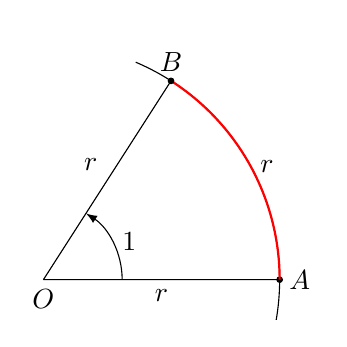
\begin{tikzpicture}
    \clip (-.2,-.5) rectangle (3.5,3.2);
    %% Horizontal
    \draw (0,0) node [below] {$O$} -- node [below] {$r$} (3,0)
    %% point A
    [fill] circle  (1pt) node [below,right] {$A$};

    %% Vue la bizarre façon de faire des arcs, plus simple de rajouter
    %% deux bouts d'arc comme ceci :
    \draw (3,0) arc (0:67:3);
    \draw (3,0) arc (0:-10:3);


    %% Arc  -- Here, 57.3 = 180/pi = 1 rad
    \draw [thick,color=red] (3,0) arc (0:57.3:3); 

    %% point B
    \draw (57.3:3) node [above] {$B$} [fill] circle  (1pt)
    %% Rayon à 1 radian.
    -- node [above left] {$r$} (0,0);

    \draw (1,0) [-latex] arc (0:57.3:1);
    \draw (0,0)
    (28.65:1) node [right] {$\SI{1}{\radian}$} %% 57.3 = 180/pi = 1 rad
    +(28.65:2) node [right] {$r$};
  \end{tikzpicture}\pause\qquad
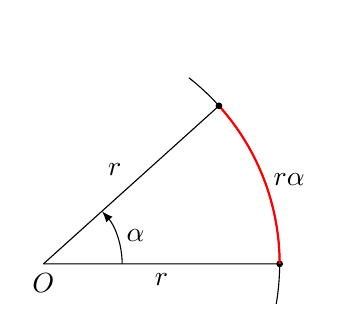
\begin{tikzpicture}
    \def\ALPHA{42}
    \clip (-.2,-.5) rectangle (3.5,3);
    %% Horizontal
    \draw (0,0) node [below] {$O$} -- node [below] {$r$} (3,0)
    %% point A
    [fill] circle (1pt);
    
    %% Vue la bizarre façon de faire des arcs, plus simple de rajouter
    %% deux bouts d'arc comme ceci :
    \draw (3,0) arc (0:\ALPHA+10:3);
    \draw (3,0) arc (0:-10:3);

    %% Arc  -- Here, \ALPHA
    \draw [thick,color=red] (3,0) arc (0:\ALPHA:3); 

    %% point B
    \draw (\ALPHA:3) [fill] circle  (1pt)
    %% Rayon à 1 radian.
    -- node [above left] {$r$} (0,0);

     \draw (1,0) [-latex] arc (0:\ALPHA:1);
     \draw (0,0)
     (.5*\ALPHA:1) node [right] {$\alpha\,\si{\radian}$} %% 57.3 = 180/pi = 1 rad
     +(.5*\ALPHA:2) node [right] {$r \alpha$};
  \end{tikzpicture}
\end{center}\pause

Le radian est idéal pour manipuler des longueurs d'arcs !
\end{frame}

\begin{frame}
  Pour passer du radian au degré et inversement, retenons que $2\pi\,\si{\radian} = \ang{360}$.\pause{} Par habitude, nous retiendrons également le tableau suivant~:\pause{}
  \begin{equation*}
    \begin{array}{l|cccccc}\toprule
      \text{en radians} & \sfrac \pi 6 & \sfrac{\pi}{4} & \sfrac{\pi}{3} & \sfrac{\pi}{2}& \pi & 2 \pi\\
      \text{en degrés} & \ang{30} & \ang{45} & \ang{60} & \ang{90} & \ang{180} & \ang{360}\\\bottomrule
    \end{array}
  \end{equation*}
\end{frame}

\subsection{Définitions de sinus, cosinus, \dots}
\label{sec:cercletrigono}\label{sec:fonctiontrigono}

\begin{frame}
  \begin{definition}
    Étant donné un angle \(\theta\) en radians,\pause{} on définit son cosinus et son sinus\pause{} comme les coordonnées du point \(P_{\theta}\)\pause{} tel que l'angle \(\widehat{IOP}\)\pause{} est de mesure \(\theta\)\pause{}, où \(I = (1,0)\) et \(O = (0,0)\).
  \end{definition}\pause

  % \begin{proposition}Pour des angles \(\theta\) et \(\varphi\), on a :
  %   \begin{equation*}
  %     \cos (\theta + \varphi) = \cos \theta \cos \varphi - \sin \theta \sin \varphi
  %   \end{equation*}
  % \end{proposition}\pause

  % Avant de prouver ce résultat, nous allons expliciter les quelques relations \og évidentes\fg{} des sinus et cosinus.
\end{frame}

\begin{frame}{Cercle trigonométrique}
  \begin{definition}
    Un \Defn{cercle trigonométrique} est un cercle de rayon $1$,\pause{} il permet de représenter géométriquement toutes les fonctions trigonométriques.\pause{}
%    Ces fonctions sont les fonctions :\pause{} sinus\pause{}, cosinus\pause{}, tangente\pause{}, cotangente\pause{}, sécante\pause{}, cosécante\pause{} et quelques autres plus rarement utilisées.
  \end{definition}

  \begin{center}
    \includegraphics[trim=0 50 0 0,clip]{fonctionstrigo}
  \end{center}
\end{frame}

\begin{frame}
  Autres fonctions trigonométriques :
  \begin{align*}
    \tan(\theta) &= \frac{\sin(\theta)}{\cos(\theta)} & %\sec(\theta) &= \frac{1}{\cos(\theta)}\\
    \cot(\theta) &= \frac{\cos(\theta)}{\sin(\theta)}% & \operatorname{cosec}(\theta) &= \frac{1}{\sin(\theta)}
  \end{align*}

%  Attention aux conditions d'existence !
\end{frame}

\begin{frame}
\begin{center}
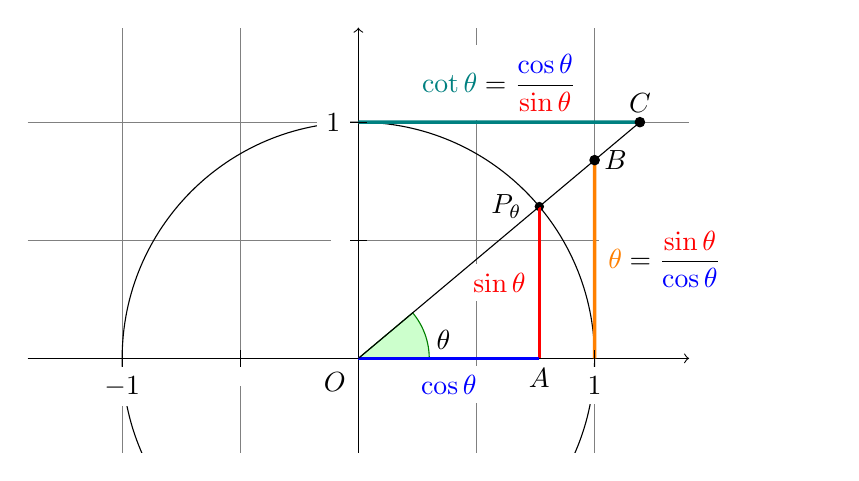
\begin{tikzpicture}[scale=3] 
\def\th{40} %% CHANGER LE CAPTION ACCORDINGLY !!
\def\diamdepoint{0.02}

\clip (-1.4,-0.4) rectangle (2,1.4);
\draw[step=0.5,gray,very thin] (-1.4,-1.4) grid (1.4,1.4);

%% petit arc vert
\filldraw[fill=green!20,draw=green!50!black] (0,0) -- (0.3,0) arc 
(0:\th:0.3) -- cycle; 
\node [right] at (15:0.3) {$\theta$};

%% Point P
\node[left=.1cm] at (\th:1) {$P_\theta$};
\fill (\th:1) circle (\diamdepoint);

%% axes
\draw[->] (-1.4,0) -- (1.4,0) coordinate (x axis); 
\draw[->] (0,-1.4) -- (0,1.4) coordinate (y axis); 

%% grand cercles
\draw (0,0) circle (1); 

%% 
\draw[very thick,red] 
(\th:1) -- node[left=1pt,fill=white] {$\sin \theta$} (\th:1 |- x axis)
coordinate (A); 
%% 
\draw[very thick,blue] 
(\th:1 |- x axis) -- node[below=2pt,fill=white] {$\cos \theta$} (0,0); 
%%
\draw[very thick,orange] (1,0) -- node [right=1pt,fill=white] 
{$\displaystyle \tg \theta \color{black}= 
\frac{{\color{red}\sin \theta}}{\color{blue}\cos \theta}$} 
(intersection of 0,0--\th:1 and 1,0--1,1) coordinate (t); 


%%
\draw[very thick,color=green!50!blue] (0,1) -- node [fill=white,above] 
{$\displaystyle \cot \theta \color{black}= 
\frac{{\color{blue}\cos \theta}}{\color{red}\sin \theta}$} 
(intersection of 0,0--\th:1 and 0,1--2,1) coordinate (c); 

\draw (0,0) -- (c) -- (t); %% Aller le plus loin : tan ou cot.
\node[right] at (t) {$B$};
\draw[fill] (t) circle (\diamdepoint);
\node[above] at (c) {$C$};
\draw[fill] (c) circle (\diamdepoint);
\foreach \x/\xtext in {-1, -0.5/{}, 1} 
\draw (\x,1pt) -- (\x,-1pt) node[anchor=north,fill=white] {$\xtext$}; 
\foreach \y/\ytext in {-1, -0.5/, 0.5/, 1} 
\draw (1pt,\y) -- (-1pt,\y) node[anchor=east,fill=white] {$\ytext$}; 
\node at (-0.1, -0.1) {$O$};
\node[below] at (A) {$A$};
\end{tikzpicture} 
\end{center}
\end{frame}

\begin{frame}{Pente et angle}
  \begin{proposition}
    Étant donné un repère cartésien \alert{orthonormé}.\pause{} Pour une droite d'équation \(y = mx + p\)\pause{} formant un angle (orienté) \(\theta\) avec l'horizontale, nous avons\pause{}
    \begin{equation*}
      m = \tan \theta
    \end{equation*}
  \end{proposition}\pause

  \begin{tabular}{lc}
  \begin{minipage}{0.3\linewidth}
    \[m = \frac{\Delta y}{\Delta x} = \frac{y_1-y_0}{x_1-x_0}\] où $(x_0, y_0)$ et $(x_1,y_1)$ sont deux points distincts du graphe de $f$.
  \end{minipage}
  \begin{minipage}{0.65\linewidth{}}
    \def\xmax{5}%
    \def\ymax{2}%
  \begin{tikzpicture}
    \draw (0,0) node [below left] {$0$};%
    \foreach \y in {1, ..., \ymax} \draw (3pt,\y) -- (-3pt,\y) node
    [left] {$\y$};%
    \foreach \x in {1, ..., \xmax} \draw (\x,3pt) -- (\x,-3pt) node
    [below] {$\x$};%
    \draw [->] (0,-.2) -- (0,\ymax+1) node [above left] {$y$};%
    \draw [->] (-.2,0) -- (\xmax+1,0) node [below right] {$x$};%
    \begin{scope}[shift={+(1,0)}]
      \draw (35:-1) -- (35:4);%
      \draw[->] (.5,0) arc (0:35:.5) node [right] {$\theta$};%
      \coordinate (A) at (35:3);%
    \end{scope}
    \draw
    [dotted]
    [postaction={%
      decorate,draw,solid,
      decoration={brace, raise=2pt}      
    }]
    (A) -- (A|-0,0) node [midway,right=3pt] {$\Delta y$};%
    \draw
    [dotted]
    [postaction={%
      decorate,draw,solid,
      decoration={brace, raise=15pt, mirror}
    }]
    (1,0) -- (A|-0,0) node [midway,below=15pt] {$\Delta x$};%
  \end{tikzpicture}
\end{minipage}
\end{tabular}
\end{frame}

\begin{frame}
  \begin{remark*}
    Cette interprétation ne tient plus si les axes ne sont
    pas gradués à l'identique :
  \end{remark*}
  %% CVV : développer car ils font régulièrement l'erreur
  %% NR : je veux bien, mais que dire d'autre si ce n'est que c'est faux en donnant un exercice à faire ? Cela dit je reformulerai la section afin d'avoir plus de clarté.
  \begin{center}
    \def\xmax{4}%
    \def\ymax{3}%
    \begin{tikzpicture}[xscale=2]
      \draw (0,0) node [below left] {$0$};%
      \foreach \y in {1, ..., \ymax} \draw (3pt,\y) -- (-3pt,\y) node
      [left] {$\y$};%
      \foreach \x in {1, ..., \xmax} \draw (\x,3pt) -- (\x,-3pt) node
      [below] {$\x$};%
      \draw [->] (0,-.2) -- (0,\ymax+1) node [above left] {$y$};%
      \draw [->] (-.2,0) -- (\xmax+1,0) node [below right] {$x$};%
      \begin{scope}[shift={+(1,0)}]
        \draw (35:-1) -- (35:4);%
        \draw[->,xscale=.5] (1,0) arc (0:19.3:1) node [right] {${\pmb ?}$};%
      \end{scope}
    \end{tikzpicture}
  \end{center}
\end{frame}

\begin{frame}{Angles remarquables}
%   Les fonctions trigonométriques les plus utilisées :
%   \begin{align*}
%   \sin &\colon \RR \vers [-1,1]\hspace*{2cm}&  \tan &\colon
%   \RR\setminus\set{\frac\pi2 + k\pi \telque k \in \ZZ} \vers \RR \\ 
%   \cos &\colon \RR \vers [-1,1]& \cot &\colon
%   \RR\setminus\set{k\pi \telque k \in \ZZ} \vers \RR.
% \end{align*}
% (L'ensemble d'arrivée a été choisi = ensemble image.)\pause

Voici quelques valeurs importantes des fonctions sinus et cosinus :
\begin{equation}\label{valeurscossin}
  \begin{array}{c|rl|c|c|c}
    \hline 
    \text{angle} & \sin & & \cos & \tan & \cot\\
    \hline
    0          &\sfrac {\sqrt 0}{2}& = 0& 1 & 0 & \nexists\\
    \sfrac \pi 6&\sfrac {\sqrt 1}{2}& = \sfrac12 &\sfrac {\sqrt 3}{2} &\sfrac {\sqrt 3}{3}& \sqrt 3\\
    \sfrac \pi 4&\sfrac {\sqrt 2}{2}& & \sfrac {\sqrt 2}{2} & 1 &1\\  
    \sfrac \pi 3&\sfrac {\sqrt 3}{2}& & \sfrac 1 2 &\sqrt 3 & \sfrac {\sqrt 3}{3}\\ 
    \sfrac \pi 2&\sfrac {\sqrt 4}{2}& = 1&0&\nexists&0\\
    \hline
  \end{array} 
\end{equation}
\end{frame}
\subsection{Relation fondamentale}
\begin{frame}
  \begin{center}
    \includegraphics[trim=0 60 0 0,clip]{fonctionstrigo}
  \end{center}
  \pause Le théorème de Pythagore\pause{} appliqué dans le cercle trigonométrique\pause{} implique l'importante relation $(\cos(\theta))^2 + (\sin(\theta))^2 = 1$,\pause{} ce qu'on écrira plus souvent sous la forme\pause{}
  \begin{equation*}
    \cos^2\theta + \sin^2 \theta  = 1.
  \end{equation*}
\end{frame}

\subsection{Symétries}
\begin{frame}{Symétrie par rapport à l'axe des abscisses}
\begin{minipage}{0.5\linewidth}
\centering
\scalebox{0.75}{\input{cercle-1.pdf_t}}
\end{minipage}
\begin{minipage}{0.45\linewidth}
\centering

\begin{align*}
\sin\paren*{ -x}&=-\sin\paren*{ x} \\
\cos\paren*{ -x}&=\cos\paren*{ x} \\ 
\tan\paren*{ -x}&=-\tan\paren*{ x}
\end{align*}
\end{minipage}
\end{frame}
\begin{frame}{Symétrie par rapport à l'axe des ordonnées}
\begin{minipage}{0.5\linewidth}
\centering
\scalebox{0.75}{\input{cercle-2.pdf_t}}
\end{minipage}
\begin{minipage}{0.45\linewidth}
\centering
\[\begin{array}{c}
\sin\paren*{ \pi -x} =\sin\paren*{ x} \\
\\
\cos\paren*{ \pi -x} =-\cos\paren*{ x} \\
\\
\tan\paren*{ \pi -x} =-\tan\paren*{ x}
\end{array}\]
\end{minipage}
\end{frame}
\begin{frame}{Symétrie par rapport à l'origine}
\begin{minipage}{0.5\linewidth}
\centering
\scalebox{0.75}{\input{cercle-3.pdf_t}}
\end{minipage}
\begin{minipage}{0.45\linewidth}
\centering
\[\begin{array}{c}
\sin\paren*{ \pi +x} =-\sin\paren*{ x} \\ \\
\cos\paren*{ \pi +x} =-\cos\paren*{ x} \\ \\
\tan\paren*{ \pi +x} =\tan\paren*{ x}
\end{array}\]
\end{minipage}
\end{frame}
\begin{frame}{Symétrie par rapport à la première bissectrice}
\begin{minipage}{0.58\linewidth}
\centering
\scalebox{0.75}{\input{cercle-4.pdf_t}}
\end{minipage}
\begin{minipage}{0.40\linewidth}
\centering
\[\begin{array}{c}
\sin\paren*{ \dfrac{\pi}{2} -x} =\cos\paren*{ x} \\ \\
\cos\paren*{ \dfrac{\pi}{2} -x} =\sin\paren*{ x} \\ \\
\tan\paren*{ \dfrac{\pi}{2} -x} =\cot\paren*{ x}
\end{array}\]
\end{minipage}
\end{frame}

\begin{frame}{Angles décalés de 90\degre}
\begin{minipage}{0.5\linewidth}
\centering
\scalebox{0.75}{\input{cercle-5.pdf_t}}
\end{minipage}
\begin{minipage}{0.45\linewidth}
\centering
\[\begin{array}{c}
\sin\paren*{ \dfrac{\pi}{2} +x} =\cos\paren*{ x} \\
\\
\cos\paren*{ \dfrac{\pi}{2} +x} =-\sin\paren*{ x} \\
\\
\tan\paren*{ \dfrac{\pi}{2} +x} =-\cot\paren*{ x}
\end{array}\]
\end{minipage}
\end{frame}

\subsection{Formules de trigonométrie}
\begin{frame}%% supprime moi
  \vspace{-3.ex}
  \begin{align*}
    \sin (A + B)      & = \sin A \cos B + \cos A \sin B                                                      \\
    \cos (A + B)      & = \cos A \cos B - \sin A \sin B                                                      \\
    \tan (A + B)      & = \frac{\tan A + \tan B}{1 - \tan A \tan B}                                          \\
    % \sin (3a) & = 3\sin a -4 \sin^{3} a \\
    % \cos (3a) & = -3\cos a +4 \cos^{3} a \\
    \cos A \cos B     & =\frac{\cos(A-B)+\cos(A+B)}2\\
    \sin A \sin B     & =\frac{\cos(A-B)-\cos(A+B)}2\\
    \sin A \cos B     & =\frac{\sin(A+B)+\sin(A-B)}2                                                        \\
    \cos A \sin B     & =\frac{\sin(A+B)-\sin(A-B)}2                                                         \\
    \cos p + \cos q   & = 2 \cos \paren*{ \frac{p+q} 2 } \cos \paren*{ \frac{p-q} 2 }                        \\
    \cos p - \cos q   & = -2 \sin \paren*{ \frac{p+q} 2 } \sin \paren*{ \frac{p-q} 2 }                       \\
    \sin p + \sin q   & = 2 \sin \paren*{ \frac{p+q} 2 } \cos \paren*{ \frac{p-q} 2 }
    % \sin p - \sin q & = 2 \cos \paren*{ \frac{p+q} 2 } \sin \paren*{ \frac{p-q} 2 } \\
  \end{align*}
\end{frame}
\course{5}
\begin{frame}
  \vspace{-3.ex}
  \begin{align*}
    \sin (A + B)      & = \sin A \cos B + \cos A \sin B                                                      \\
    \cos (A + B)      & = \cos A \cos B - \sin A \sin B                                                      \\
    \tan (A + B)      & = \frac{\tan A + \tan B}{1 - \tan A \tan B}                                          \\
    % \sin (3a) & = 3\sin a -4 \sin^{3} a \\
    % \cos (3a) & = -3\cos a +4 \cos^{3} a \\
    \cos A \cos B     & =\frac{\cos(A-B)+\cos(A+B)}2\\
    \sin A \sin B     & =\frac{\cos(A-B)-\cos(A+B)}2\\
    \sin A \cos B     & =\frac{\sin(A+B)+\sin(A-B)}2                                                        \\
    % \cos A \sin B     & =\frac{\sin(A+B)-\sin(A-B)}2                                                         \\
    \cos p + \cos q   & = 2 \cos \paren*{ \frac{p+q} 2 } \cos \paren*{ \frac{p-q} 2 }                        \\
    \cos p - \cos q   & = -2 \sin \paren*{ \frac{p+q} 2 } \sin \paren*{ \frac{p-q} 2 }                       \\
    \sin p + \sin q   & = 2 \sin \paren*{ \frac{p+q} 2 } \cos \paren*{ \frac{p-q} 2 }
    % \sin p - \sin q & = 2 \cos \paren*{ \frac{p+q} 2 } \sin \paren*{ \frac{p-q} 2 } \\
  \end{align*}\pause
  Les deux premières formules sont à connaître.
\end{frame}
\begin{frame}
  \begin{proof}[Preuve de la formule d'addition]
    Nous voulons prouver
    \begin{math}
      \cos (\theta + \varphi) = \cos \theta \cos \varphi - \sin \theta \sin \varphi.
    \end{math}\par\pause
    \begin{minipage}{0.66\linewidth}
      Dans un repère cartésien, notons\pause{}
      \begin{itemize}
      \item \(\vec{o} = (0,0)\),\pause{} \(\vec{a} = (1,0)\),\pause{} \(\vec{b} = (0,1)\),\pause{}
      \item \(
        \begin{aligned}[t]
          \vec{p} &= % (\cos(\theta),\sin(\theta))= 
          \cos(\theta) \vec{a} + \sin(\theta) \vec{b}
        \end{aligned}\)\pause{}
      \item \(\vec{q} = (\cos(\theta + \varphi),\sin(\theta + \varphi))\)\pause{}
      \item \(
        \begin{aligned}[t]
          \vec{r} &= (\cos(\theta + \pi/2),\sin(\theta + \pi/2))\\
          &= (-\sin(\theta),\cos(\theta))
        \end{aligned}\)
      \end{itemize}\pause{}
    \end{minipage}
    \begin{minipage}{0.33\linewidth}
      \includegraphics[width=\linewidth]{cosdesomme}
    \end{minipage}\pause

    Dans le repère tourné d'un angle \(\theta\), on observe\pause{}
    \begin{math}
      \vec{q} = \cos(\varphi) \vec{p} + \sin(\varphi)\vec{r},
    \end{math}\pause{}
    et donc\pause{}
%    \vspace*{-2.5ex}
    \begin{align*}
      (\cos(\theta& + \varphi),\sin(\theta + \varphi))\\
      &= \cos(\varphi) \, (\cos(\theta),\sin(\theta)) + \sin(\varphi) \, (-\sin(\theta),\cos(\theta))\\
      &= (\cos(\varphi) \cos(\theta) - \sin(\varphi) \sin(\theta), \cos(\varphi) \sin(\theta) + \sin(\varphi)\cos(\theta))
    \end{align*}
    ce qui démontre la relation proposée, ainsi que la relation similaire concernant \(\sin(\varphi+\theta)\).
  \end{proof}
\end{frame}

\subsection{Lois trigonométriques}
\begin{frame}{Trigonométrie dans les triangles}
  Rappelons que si $ABC$ est un triangle, rectangle en $A$, alors :\pause
  \begin{align*}
    \uncover<+->{\sin(\hat B) &= \frac{AC}{BC} &}
    \uncover<+->{\cos(\hat B) &= \frac{AB}{BC} &}
    \uncover<+->{\tan(\hat B) &= \frac{AC}{AB}}
  \end{align*}
\end{frame}

\begin{frame}{Loi des sinus}
  \begin{minipage}{0.49\linewidth}
  Soit un triangle de sommets \(A,B,C\) tel que représenté ci-contre, \uncover<2->{alors :
  \begin{equation*}
    \frac{\sin \hat A}{a} = \frac{\sin\hat B}{b} = \frac{\sin\hat C}{c}
  \end{equation*}}
\end{minipage}
\begin{minipage}{0.49\linewidth}
  \uncover<1->{\includegraphics{triangleqcq}}
\end{minipage}
  \begin{proof}\pause
    Prouvons l'une de ces égalités :\pause

    Notons \(h\) la hauteur issue de \(B\).\pause{} Alors d'une part \(\sin \hat{C} = \frac{h}{a}.\)\pause{} et d'autre part \(\sin \hat{A} = \frac{h}{c}\),\pause{} ceci prouve
    \begin{equation*}
      \frac{\sin \hat A}{a} =  \frac{\sin\hat C}{c}
    \end{equation*}
  \end{proof}
\end{frame}

%\subsection{Loi des cosinus}
\begin{frame}{Loi des cosinus}
\vspace*{-1\baselineskip}
  \begin{minipage}{0.59\linewidth}
    Soit un triangle de sommets \(A,B,C\) tel que représenté ci-contre, \uncover<2->{alors :
  \begin{equation*}
    c^{2} = a^{2} + b^{2} - 2 a b \cos \hat{C}
  \end{equation*}}
  \uncover<3->{Ceci est un théorème de Pythagore généralisé}
\end{minipage}
\begin{minipage}{0.39\linewidth}
  \uncover<1->{\includegraphics[width=\linewidth]{triangleqcq}}
\end{minipage}
\pause

Pour prouver cette relation, nous allons introduire quelques outils. 
\begin{block}{Note a posteriori}
  Nous n'avons finalement pas prouvé la relation au cours. Le lecteur curieux trouvera la preuve dans le syllabus en fin de chapitre Trigonométrie.
\end{block}
% \begin{proof}\pause\pause
%     Notons \(\vec{AC} = \point{C} - \point{A}\) pour le vecteur de \(\point{A}\) à \(\point{C}\), etc.\pause et développons \(c^{2}\) grâce au produit scalaire :
%     \begin{align*}
%       \uncover<+->{c^{2} &= \norme{\vec{AB}}^{2} = \norme{\vec{AC} + \vec{CB}}^{2}}
%       \uncover<+->{= \norme{\vec{AC}}^{2} + \norme{\vec{CB}}^{2} + 2 \scalprod{\vec{AC}}{\vec{CB}} \\}
%       \uncover<+->{&= \norme{\vec{AC}}^{2} + \norme{\vec{CB}}^{2} + 2 \norme{\vec{AC}} \norme{\vec{CB}} \cos(\pi - \hat{C})\\}
%       \uncover<+->{&= \norme{\vec{AC}}^{2} + \norme{\vec{CB}}^{2} - 2 \norme{\vec{AC}} \norme{\vec{CB}} \cos(\hat{C})}
%     \end{align*}\pause
%   Attention, l'angle entre \(\vec{AC}\) et $\vec{CB}$ est \(\pi - \hat{C}\) car ils n'ont pas le même point base sur l'image. 
%   \end{proof}
\end{frame}

\begin{frame}
  \begin{definition}
    Le \Defn{produit scalaire} entre deux vecteurs \(\vec v\) et \(\vec w\) de \(\RR^{n}\) est donné par
    \begin{equation*}
      \scalprod {\vec v} {\vec w} = v_{1} w_{1} + \cdots + v_{n} w_{n}.
    \end{equation*}
  \end{definition}

  \begin{example}
    \begin{equation*}
      \scalprod{(2,1)}{(2,5)} = 2 \cdot 2 + 1 \cdot 5 = 9
    \end{equation*}\pause
    \begin{align*}
      \uncover<+->{\scalprod{(1,0)}{(2,5)} &= 2&}
      \uncover<+->{\scalprod{(0,1)}{(2,5)} &= 5&}
      \uncover<+->{\scalprod{(1,1)}{(2,5)} &= 7}
    \end{align*}\pause
    Notons que si \(\vec{v} = (v_{1},v_{2}, \ldots, v_{n})\)\pause{}, alors \(\scalprod{\vec{v}}{\vec{e_{i}}} = v_{i}\)

    Où :
  \(\paren{e_{i}}_{j} =
    \begin{cases}
      1 & \text{si \(i = j\)} \\
      0 & \text{sinon.}
    \end{cases}
    \qquad \vec{e_{i}} = (0,\ldots,0,{\underbrace{1}_{\mathclap[\displaystyle]{\text{\(i\)-ème pos}}}},0,\ldots,0)\)
\end{example}
\end{frame}
\begin{frame}
  \begin{proposition}Pour tous vecteurs \(\vec a,\vec {a'},\vec b \in \RR^{n}\) et \(\lambda, \mu \in \RR\),\pause{} le produit scalaire vérifie les propriétés suivantes :\pause{}
    \begin{enumerate}
    \item $\scalprod{\vec{a}}{\vec{b}}=\pause\scalprod{\vec{b}}{\vec{a}}$ (symétrique)\pause{}
    \item $\scalprod{\vec{a}}{\vec{a}} \geq 0$\pause{} et de plus, $\scalprod{\vec{a}}{\vec{a}} = 0 \iff \vec{a} = \vec 0$ (défini positif).
    \item $\scalprod{(\lambda \vec{a} + \mu \vec{a'})}{\vec{b}} = \pause \lambda \scalprod{\vec{a}}{\vec{b}} + \mu \scalprod{\vec{a'}}{\vec{b}}$.
    \end{enumerate}
  \end{proposition}\pause{}
  La dernière propriété est une forme de distributivité appelée "linéarité à gauche".\pause{} Au vu de la symétrie\pause{}, on a aussi "linéarité à droite",\pause{} ce qui s'appelle alors "bilinéarité".
  \pause{}
\end{frame}

\begin{frame}
  On définit la \Defn{norme} (associée à ce produit scalaire) par :
  \begin{equation*}
    \norme {\vec v} \pardef \sqrt{\scalprod{\vec v}{\vec v}} = \sqrt{v_{1}^{2}  + \cdots + v_{n}^{2}}
  \end{equation*}\pause
  Cette norme vérifie donc la propriété \(\norme{\vec v} = 0 \iff \vec v = 0\).\pause

  \begin{remark*}
    La \og norme\fg{} d'un vecteur correspond à sa \og longueur\fg{} d'après le théorème de Pythagore.
  \end{remark*}\pause

  \begin{example}
    (pour \(n = 2\)) Si \((a,b) \in \RR^2\),\pause{} on a \(\norme{(a,b)} =\pause \sqrt{a^{2} + b^{2}}\).
  \end{example}
\end{frame}

\begin{frame}
  \begin{proposition}[Inégalité de Cauchy-Schwarz]Pour tout \(\vec a, \vec b\) de \(\RR^{n}\), on a 
    \begin{equation*}
      \abs{\scalprod{\vec a}{\vec b}} \leq \norme {\vec a} \norme {\vec b}.
    \end{equation*}
  \end{proposition}
\end{frame}
\begin{frame}
  \begin{proof}
    Considérons la quantité \(\scalprod{\vec a + t \vec b}{\vec a + t \vec b}\), qui est positive.
    \pause Nous pouvons la ré-écrire via la bilinéarité du produit scalaire sous la forme~:\pause
    \begin{align*}
      \uncover<+->{\scalprod{\paren*{\vec a + t \vec b}}{\paren*{\vec a + t \vec b}}}
      \uncover<+->{&= \scalprod {\vec a}{\vec a} + 2 t \scalprod{\vec a}{\vec b} + t^{2} \scalprod{\vec b}{\vec b}\\}
      \uncover<+->{&= \norme{\vec{a}}^{2} + 2 t \scalprod {\vec a}{\vec b} + t^{2} \norme{\vec{b}}^{2} \\}
      \uncover<+->{&= \paren*{t \norme{\vec{b}} + \frac{\scalprod{\vec a}{\vec b}}{\norme{\vec{b}}}}^{2} - \paren*{\frac{\scalprod{\vec a}{\vec b}}{\norme{\vec{b}}}}^{2} + \norme{\vec{a}}^{2} \geq 0}
    \end{align*}\pause
    En choisissant \(t = - \frac{\scalprod {\vec a}{\vec b}}{\norme{\vec{b}}^{2}}\), on obtient\pause{}
    \begin{math}
      \norme{\vec{a}}^{2} \geq \paren*{\frac{{\scalprod{\vec a}{\vec b}}}{\norme{\vec{b}}}}^{2},
    \end{math}\pause
    d'où
    \begin{equation*}
      \norme{\vec{a}} \geq \frac{\abs{\scalprod{\vec a}{\vec b}}}{\norme{\vec{b}}}
    \end{equation*}
    qui est l'inégalité annoncée.
  \end{proof}
\end{frame}
\begin{frame}
  \begin{proposition}
    La norme \(\norme \cdot : \RR^{n} \to \RR\) vérifie les propriétés suivantes~:
    \begin{itemize}
    \item \(\norme{\vec a} = 0 \iff \vec a = \vec 0\) ;
    \item \(\norme{\lambda \vec a} = \abs \lambda \norme{\vec a}\) ;\pause
    \item \(\norme{\vec a + \vec b} \leq \norme{\vec a} + \norme{\vec b}\) (inégalité triangulaire).
    \end{itemize}
  \end{proposition}\pause
  \begin{proof}[La preuve est omise]
    % Les deux premières propriétés sont évidentes de la définition de la norme et les propriétés du produit scalaire. \pause La troisième se démontre en calculant
    % \begin{align*}
    %   \uncover<+->{\norme{\vec a + \vec b}^{2}}
    %   \uncover<+->{&= \scalprod{\vec a + \vec b}{\vec a + \vec b}\\}
    %   \uncover<+->{& = \scalprod{\vec a}{\vec a} + \scalprod{\vec b}{\vec b} + 2 \scalprod{\vec a}{\vec b} \\}
    %   \uncover<+->{& \leq \scalprod{\vec a}{\vec a} + \scalprod{\vec b}{\vec b} + 2 \norme{\vec a}\norme{\vec b}\\}
    %   \uncover<+->{&= \paren*{\norme {\vec a} + \norme {\vec b}}^{2}}
    % \end{align*}
    % où nous avons utilisé l'inégalité de Cauchy-Schwarz.
  \end{proof}
\end{frame}
\begin{frame}
  \begin{proposition}
    Si \(\vec v\) et \(\vec w\) sont des vecteurs de \(\RR^{n}\), alors\pause{}
    \begin{equation*}
      \scalprod{\vec v}{\vec w} = \norme {\vec v}\norme{\vec w} \cos(\theta)
    \end{equation*}\pause{}
    où \(\theta\) est l'angle orienté formé par les vecteurs \(\vec v\) et \(\vec w\) (supposés basés au même point!).
  \end{proposition}\pause
  \begin{remark}
    Si \(\vec{v}\) est un vecteur quelconque,\pause{} alors \(\frac{\vec{v}}{\norme{v}}\) est de norme \(1\),\pause{} et donc de la forme \((\cos\phi,\sin\phi)\) pour un certain angle \(\phi\).
  \end{remark}\pause
  \begin{proof}[Preuve de la proposition en dimension \(2\)]
    Si \(\vec v = (\norme {\vec v} \cos(\phi), \norme {\vec v} \sin(\phi))\)\pause{} et  \(\vec w = (\norme {\vec w} \cos(\psi), \norme {\vec w} \sin(\psi))\),\pause{} alors 
    \begin{equation*}
      \scalprod{\vec v}{\vec w} =\pause \norme{\vec v}  \norme{\vec w} (\cos(\phi)\cos(\psi) + \sin(\phi)\sin(\psi)) =\pause \norme{\vec v}\norme{\vec w} \cos{\paren{\psi-\phi}}
    \end{equation*}
    où \(\psi-\phi\) représente bien l'angle entre les deux vecteurs.
  \end{proof}
\end{frame}

\begin{frame}
  \begin{corollary}
    Le produit scalaire s'annule si et seulement si les vecteurs sont orthogonaux (ou si l'un des deux vecteurs est nul).\pause{}
  \end{corollary}
  \begin{proof}
    Rappelons le résultat :
    \begin{equation*}
      \scalprod{\vec v}{\vec w} = \norme {\vec v}\norme{\vec w} \cos(\theta)
    \end{equation*}\pause{}

    Si les vecteurs ne sont pas nuls, alors leur norme n'est pas nulle\pause{}, dès lors seul le cosinus peut s'annuler\pause{}, ce qui n'arrive que pour des angles droits.\pause{}
  \end{proof}
\end{frame}

\begin{frame}
  \begin{corollary}La projection orthogonale d'un vecteur \(\vec{v}\) sur un vecteur \(\vec{w}\) (basé au même point) est\pause{}
    \(\vec p = \frac{\scalprod{\vec{v}}{\vec{w}}}{\norme{w}^{2}} \vec{w}\).
  \end{corollary}\pause
  \begin{proof}
    Le projeté sera du type \(\vec{p} = k \vec{w}\) pour un certain \(k\).\pause
    
    On veut que \(\vec{v} - \vec{p}\) soit orthogonal à \(\vec{w}\).\pause

    On écrit l'égalité correspondante, et la valeur de \(k\) en découle :\pause{}

    \begin{equation*}
      \scalprod{\vec{v}-\vec{p}}{\vec{w}} = 0 \iff\pause \scalprod{\vec{v}}{\vec{w}} =\pause \scalprod{k\vec{w}}{\vec{w}} =\pause k \norme{\vec{w}}^{2}
    \end{equation*}
  \end{proof}
\end{frame}

\section{Fonctions}
\begin{frame}
  \begin{definition}
    Se donner une \Defn{fonction} $f$\pause{} s'est se donner :
    \begin{itemize}
    \item un \Defn{ensemble de départ} $A$,\pause{}
    \item un \Defn{ensemble d'arrivée} $B$ et\pause{}
    \item une règle permettant d'associer à chaque élément $x$ de $A$\pause{} un unique élément de $B$ noté \(f(x)\).
    \end{itemize}

    \begin{itemize}
    \item \(f(x)\) est l'\Defn{image} de $x$ par $f$.\pause{}
    \item On dit aussi que \(x\) est un \Defn{antécédent} de \(f(x)\).
    \end{itemize}\pause{}

    La notation pour une fonction $f$ de $A$ dans $B$ est\pause{}
    \begin{equation*}
      f : A \to B : x \mapsto f(x)
    \end{equation*}
  \end{definition}
\end{frame}

\begin{frame}
\begin{example}Voici quelques exemples de fonctions :\pause{}
  \begin{itemize}[<+->]
  \item Une fonction associant à chaque réel son carré
    \begin{equation*}
      g : \RR \to \RR : x \mapsto x^2 ;
    \end{equation*}
  \item la fonction valeur absolue
    \begin{equation*}
      h : \RR \to \RR : x \mapsto \abs x ;
    \end{equation*}
  \item la fonction \Defn{plancher}
    \begin{equation*}
      i : \RR \to \ZZ : x \mapsto \lfloor x \rfloor
    \end{equation*}
    où $\lfloor x \rfloor$ est défini comme le plus grand entier $k$ tel que $k \leqslant x$;
  \end{itemize}
\end{example}
\end{frame}

\begin{frame}
  \begin{example}
    \begin{itemize}[<+->]
    \item la \Defn{fonction caractéristique} de l'ensemble \(\QQ \subset \RR\)
      \begin{equation*}
        j : \RR \to \{0,1\} : x \mapsto 
        \begin{cases}
          1 &\text{si } x \in \QQ\\
          0 &\text{si } x \in \RR \setminus \QQ
        \end{cases}
      \end{equation*}
    \end{itemize}
  \end{example}
\end{frame}
\begin{frame}
  \frametitle{Autres exemples de fonction}
  \begin{example}
    Si $t$ désigne le nombre de secondes depuis un instant $0$ fixé arbitrairement\pause{}, nous pouvons noter $f(t)$\pause{}
    \begin{itemize}[<+->]
    \item le nombre de lapins sur le campus Plaine, ou
    \item le nombre de bactéries dans environnement donné, ou
    \item toute quantité dont les variations au fil du temps nous intéresse\dots
    \end{itemize}
  \end{example}
\end{frame}

\begin{frame}
  Une fonction peut concerner autre chose que des nombres.
  \begin{example}
    Soit \(A\) l'ensemble des étudiants à l'ULB,\pause{} soit \(B\) l'ensemble des nombres naturels.\pause{} On associe, à chaque étudiant, son numéro matricule.\pause{} Chaque étudiant à l'ULB possède un unique tel numéro matricule, cela définit donc une fonction.
  \end{example}\pause
  \begin{example}La notation
    \begin{equation*}
      f : \RR \to \RR : x \mapsto \frac{1}{x}
    \end{equation*}
    ne définit \emph{pas} une fonction au sens précédent, car l'image de \(0\) n'a pas été définie.\pause{} Par contre,
    \begin{equation*}
      g : \RR \to \RR : x \mapsto
      \begin{cases*}
        \frac{1}{x} & si \(x \neq 0\)\\
        0 & sinon.
      \end{cases*}
    \end{equation*}
    définit correctement une fonction.
  \end{example}
\end{frame}

\subsection{Définitions}
\begin{frame}
  \begin{exercise}
    Comment choisir le domaine \(A \subset \RR\)\pause{} pour que
    \begin{equation*}
      f : A \to \RR : x \mapsto \frac{1}{x^{2}-1}
    \end{equation*}
    définisse une fonction ?\pause{}

    \begin{answer}
    N'importe quel \(A\) ne contenant ni \(1\) ni \(-1\) convient.\pause{} Généralement, nous prenons \og le plus grand possible\fg{},\pause{} c'est-à-dire \(A = \RR\setminus\set{-1,1}\).
  \end{answer}

    %% FIXMEs: on peut le représenter comme suit:

    %% dans ce cas le graphe est: ...

    %% mais on pourrait aussi choisir par exemple \interoo{-1,1}, représenté comme suit:

    %% dans ce cas le graphe est: ...
  \end{exercise}\pause
  \begin{remark*}
    On l'a vu : la règle qui donne $f(x)$ est souvent une simple formule contenant la variable~$x$\pause{} (également appelée \Defn{expression algébrique}).\pause{} Mais parfois la recette est plus complexe, et parfois il n'y a aucune formule.\pause{}
  \end{remark*}
\end{frame}



\begin{frame}{Graphe de fonction}
  \begin{definition}
    Le graphe d'une fonction \(f : A\subset \RR\to\RR\)\pause{} est l'ensemble des couples du plan\pause{} de la forme \((x,f(x))\).
  \end{definition}\pause{}
  Par définition, il s'agit donc des solutions de l'équation $y = f(x)$.\pause{}

  \begin{center}
  \begin{tikzpicture}[xscale=2,yscale=.9] %% Warning : bad practice
    %% inside (modif of xscale to kill the
    %% global effect)
    \draw (0,0) node [below left] {$0$};%
    \foreach \y in {1, ..., 4} \draw[xscale=.5] (3pt,\y) -- (-3pt,\y)
    node [left] {$\y$};%
    \foreach \x in {-2, -1, 1, 2} \draw (\x,-3pt) node [below] {$\x$} --
    (\x,3pt);%
    \draw [->] (0,-.2) -- (0,4.9) node [left] {$y$};%
    \draw [->] (-2.2,0) -- (3,0) node [below right] {$x$};%

    % \draw[xscale=.5,ultra thick] (0,0) [fill] circle (2pt) -- (0,4)
    % circle (2pt);%
    \draw (0,0) parabola[bend at start] +(2,4) node
    [right] {$y = x^2$};
    \draw (0,0) parabola[bend at start] +(-2,4);
    \draw [dashed] (1.5,0) -- (1.5,2.25) -- (0,2.25);
  \end{tikzpicture}
\end{center}
\end{frame}

\begin{frame}
  \begin{definition}
    Une fonction $f \colon A \to B$, avec $A \subset \RR$ et $B \subset \RR$ est~:\pause{}
    \begin{itemize}
    \item \Defn{paire}\pause{} si et seulement si pour tout $x$ de $A$,\pause{} on a $-x \in A$ et $f(x) = f(-x)$.
    \item \Defn{impaire}\pause{} si et seulement si pour tout $x$ de $A$,\pause{} on a $-x \in A$ et $f(-x) = -f(x)$.
    \end{itemize}
  \end{definition}
  \begin{remark*}\pause{}
    Une fonction est paire \(\iff\)\pause{} son graphe est symétrique par rapport à l'axe des ordonnées.\pause{}

    Une fonction est impaire \(\iff\)\pause{} son graphe est symétrique par rapport à l'origine $(0,0)$.
  \end{remark*}
\end{frame}
\course{6}
\begin{frame}
  Soit $f : A \to B$ une fonction.\pause{}
  \begin{itemize}
  \item $f$ est \Defn{surjective} si\pause{} tout élément de $B$ est l'image d'au moins un élément de $A$ ;\pause{}
  \item $f$ est \Defn{injective} si\pause{} deux éléments distincts de $A$ ont des images distinctes ;\pause{}
  \item $f$ est \Defn{bijective} si\pause{} $f$ est à la fois injective et surjective.
  \end{itemize}\pause

  \begin{remark}
    Une fonction est injective si et seulement si\pause{} toute droite horizontale coupe son graphe en \emph{maximum} un point !
  \end{remark}
\end{frame}

\begin{frame}
  Soit \(f : A \to B\) une fonction.\pause{}
  L'ensemble image de \(f\), noté \(\im f\) ou \(f(A)\), est l'ensemble \(\set{f(x) \telque x \in A}\).\pause{}

  L'ensemble image de la fonction\dots\pause{}
  \begin{itemize}
  \item \(f : \RR \to \RR : x \mapsto x^{2}\) est\pause{} \(\RR^+\)\pause
  \item \(f : \RR \to \RR : x \mapsto x^{3}\) est\pause{} \(\RR\)
  \end{itemize}
\end{frame}

\begin{frame}
  Le graphe de $[0,2] \to \RR : x \mapsto x^2$  et son ensemble image\pause
  \begin{center}
    \begin{tikzpicture}[xscale=2,yscale=1] %% Warning : bad practice
      %% inside (modif of xscale to kill the
      %% global effect)
      \draw (0,0) node [below left] {$0$};%
      \foreach \y in {1, ..., 5} \draw[xscale=.5] (3pt,\y) -- (-3pt,\y) node [left] {$\y$};%
      \foreach \x in {1, 2} \draw (\x,-3pt) node [below] {$\x$} -- (\x,3pt);%
      \draw [->] (0,-.2) -- (0,6) node [above left] {$y$};%
      \draw [->] (-.2,0) -- (3,0) node [below right] {$x$};%

      \draw[xscale=.5,ultra thick] (0,0) [fill] circle (2pt) -- (0,4) circle (2pt);%
      \draw (0,0) parabola[bend at start] +(2,4) node [right] {$y = x^2$}; \draw [dashed] (2,0) -- (2,4) -- (0,4);
    \end{tikzpicture}
  \end{center}
\end{frame}

% \begin{frame}
%   \begin{definition}
%     Une \Defn{fonction réelle} est une fonction dont le domaine et l'ensemble d'arrivée sont un sous-ensemble de \(\RR\).
%   \end{definition}

%   \begin{remark*}
%     Le graphe d'une fonction réelle peut être dessiné dans le plan. Pour les autres fonctions, le graphe est simplement un ensemble de couples :
%     \begin{equation*}
%       \set{ (x, f(x)) \telque x \in \dom f } 
%     \end{equation*}
%   \end{remark*}
% \end{frame}

\begin{frame}{Injectivité, surjectivité et graphe}
  \begin{remark}
    \begin{itemize}
    \item On peut \og voir\fg{} les antécédents d'un nombre \(y\) sur le graphe de \(f\) en traçant une droite horizontale à hauteur \(y\)\pause{} : les antécédents sont les abcisses des points d'intersection.\pause{} Pour la hauteur \(y = 2.25\) :\pause{}
      \begin{center}
        \includegraphics[height=4cm]{graphe-xcarre}
      \end{center}\pause{}
    \item Une fonction est injective si et seulement si\pause{} tout élément dans son ensemble d'arrivée admet au maximum un antécédent.\pause{}
    \item Une fonction est surjective si et seulement si\pause{} tout élément dans son ensemble d'arrivée admet au moins un antécédent.
    \end{itemize}
  \end{remark}
\end{frame}

\subsection{Classes de fonctions}
\begin{frame}{Fonctions polynomiales}
  \begin{definition}
    Les \Defn{fonctions polynômiales}\pause{} sont des fonctions de la forme
    \begin{equation*}
      x \mapsto a_0 + a_1 x + a_2 x^2 + \cdots + a_n x^n
    \end{equation*}\pause{}
    où $a_0, \ldots, a_n$ sont des constantes réelles\pause{}, et $n$ est un entier.\pause

    L'entier \(n\) est le \Defn{degré} de la fonction (si $a_n \neq 0$).
  \end{definition}\pause
\end{frame}

\begin{frame}{Fonctions racines}
  \begin{example}
    Les fonctions \emph{racine carrée} et \emph{racine cubique} sont~:
    \begin{equation*}
      \RR^+ \to \RR^{+} : x \mapsto \sqrt{x} \quad \text{et} \quad  \RR \to \RR : x \mapsto \sqrt[3]{x}
    \end{equation*}
  \end{example}\pause

  \begin{example}
    Plus généralement, pour \(n\) naturel pair, nous avons une fonction racine \(n\)\ieme{}~:
    \begin{equation*}
      \RR^+ \to \RR^{+} : x \mapsto \sqrt[n]{x}
    \end{equation*}
    et pour \(n\) naturel impair, similairement avec un autre domaine~:
    \begin{equation*}
      \RR \to \RR : x \mapsto \sqrt[n]{x}.
    \end{equation*}
  \end{example}
\end{frame}

\begin{frame}
  \begin{center}
    \includegraphics{racines-carree}
  \end{center}\pause{}

  La fonction racine carrée est en rouge.\pause{}
  En noir, c'est la fonction $x \mapsto x^{2}$.
\end{frame}
\begin{frame}
  \begin{center}
    \includegraphics{racines-cubique}
  \end{center}
\end{frame}

\begin{frame}{Croissance et décroissance}
  \begin{definition}
    Soit \(f\) une fonction réelle et \(A \subset \dom f\).\pause{} Cette fonction est\pause{}
    \begin{itemize}[<+->]
    \item \Defn{croissante} sur \(A\) si\pause{} pour tout \(x, y\) dans \(A\) : \(x \leq y \Rightarrow f(x) \leq f(y)\) ;\pause{}
    \item \Defn{décroissante} sur \(A\) si\pause{} pour tout \(x, y\) dans \(A\) : \(x \leq y \Rightarrow f(x) \geq f(y)\) ;\pause{}
    \item \Defn{strictement croissante} sur \(A\) si\pause{} pour tout \(x, y\) dans \(A\) : \(x < y \Rightarrow f(x) < f(y)\) ;\pause{}
    \item \Defn{strictement décroissante} sur \(A\) si\pause{} pour tout \(x, y\) dans \(A\) : \(x < y \Rightarrow f(x) > f(y)\).
    \end{itemize}
  \end{definition}
\end{frame}
\begin{frame}
  \(x \mapsto x^{2}\) est décroissante sur \(\RR^{-}\) et croissante sur \(\RR^+\) :\pause{}
  \begin{center}
    \includegraphics[height=4cm]{graphe-xcarre}
  \end{center}
  \pause Sur \(\RR\), elle n'est ni croissante ni décroissante\pause{} ; on dit qu'elle n'est pas monotone.
\end{frame}

\subsection{Les fonctions exponentielles et logarithmes}\label{fctlog}
\begin{frame}{Exponentielles}
  \begin{definition}
    Les fonction exponentielles sont les fonctions du type\pause{}
    \begin{equation*}
      f : \RR \to \RR : x \mapsto a^x
    \end{equation*}\pause{}
    pour un certain réel positif $a > 0$, appelé la \Defn{base} de l'exponentielle.
  \end{definition}\pause

  \begin{definition}
    \emph{La} fonction exponentielle\pause{}, c'est la fonction exponentielle dont la base est $a = \textup{e}$, où $\textup{e} \simeq 2.7182818\ldots$ est une constante appelée\dots \og le nombre $\textup{e}$.\fg{} %% todo : lien avec Euler ou pas ?
  \end{definition}\pause
  
  \begin{remark}
    \begin{itemize}
    \item Domaine = $\RR$ \qquad Image = $\RR_0^+ = \mathopen]0,\infty\mathclose]$.\pause{}
    \item Si \(a > 1\), l'exponentielle est croissante !\pause{}
    \item Si \(0 < a < 1\), l'exponentielle est décroissante !
    \end{itemize}
  \end{remark}
\end{frame}

\begin{frame}{Graphe}
  La ligne rouge est la ligne intéressante pour l'instant :\pause{}
  \begin{center}
    \pgfuseimage{explog}
  \end{center}
\end{frame}

\begin{frame}{Logarithme}
  \begin{question}
    Quel est le nombre \(x\) tel que \(100000000 = 10^x\) ?
  \end{question}\pause
  \begin{definition}
    Le logarithme de \(y\) en base \(a\) est le nombre \(x\) tel que \(a^{x} = y\) ! On le note \(\log_{a}(y)\).
  \end{definition}
  \pause
  \begin{equation*}
    \log_a (y) = x \iff a^{x} = y
  \end{equation*}
  \pause
  \begin{remark*}
    En d'autres termes, le logarithme de \(y\) en base \(a\) est l'antécédent de \(y\) pour la fonction \(x\mapsto a^{x}\)
  \end{remark*}
\end{frame}

\begin{frame}{Graphe}
  Revenons aux graphes :\pause{}
  \begin{center}
    \pgfuseimage{explog}
  \end{center}
\end{frame}

\begin{frame}
  Les fonctions logarithmes sont définies sur le domaine $\RR_0^+$ et ont pour ensemble image $\RR$.
  \pause
  
  Il y a quelques fonctions logarithmes fort utilisées :\pause{}
  \begin{itemize}
  \item le logarithme décimal, en base $10$, souvent noté simplement $\log$,\pause{}
  \item le logarithme en base $e$, souvent noté $\ln$, et\pause{}
  \item le logarithme en base $2$, noté $\log_{2}$.
  \end{itemize}
\end{frame}

\begin{frame}{Identités importantes}\label{expologimportantid}
  \begin{proposition}
    Pour $a, b > 0$ et $x, y \in \RR$.
    \begin{itemize}
    \item $\exp\paren{{\ln a}} = a$ et $\ln(\exp x) = x$,\pause{}
    \item $\exp (0) = 1$ et $\ln 1 = 0$,\pause{}
    \item $\exp\paren{x+y} = \exp x \exp y$\pause{} et $\ln(a b) = \ln(a) + \ln(b)$,\pause{}
    \item $\ln (a^x) = x \ln a$\pause{}
    \item $\log_{a}(b) = \frac{\ln(b)}{\ln(a)}$.
    \end{itemize}
  \end{proposition}
\end{frame}
\section{Équations et systèmes}
\begin{frame}
\begin{definition}
  Une \Defn{équation} est une égalité faisant intervenir une ou plusieurs quantités inconnues.\pause

  Résoudre une équation revient à déterminer l'ensemble des valeurs possibles pour la quantité inconnue de sorte que l'égalité soit vérifiée. Ces valeurs sont les \Defn{solutions} de l'équation.
\end{definition}

Dans une de ses formes les plus simples, une équation fait intervenir une unique quantité inconnue : un nombre réel. La \og quantité inconnue\fg{} (ou simplement \og inconnue\fg{}) est souvent nommée \(x\), mais ce nom n'a rien de magique.
\end{frame}
\begin{frame}
\begin{example}
  \begin{itemize}[<+->]
  \item L'équation \(2x - 3 = 1\) a pour seule solution : \(x = 2\).
  \item L'équation \(t^{2} - 1 = 0\) (dont l'inconnue est \(t\)) a pour solutions : \(t = 1\) et \(t = -1\). On peut écrire que l'ensemble des solutions est \(S = \set{-1,1}\).
  \item L'équation \(\sin(x) = 0\) a pour solution \(x = 0\), mais il y en a d'autres. \pause Par exemple \(x = \pi\). \pause En fait, l'ensemble des solutions est formé de l'ensemble des multiples entiers de \(\pi\). On peut noter \(S = \set{k \pi \telque k \in \ZZ}\).
  \item L'équation \(x^{2} + 1 = 0\) n'a pas de solution dans les nombres réels, car tout réel pris au carré est positif, donc \(x^{2}+1\) ne peut jamais être égal à \(0\). L'ensemble des solutions est donc vide. On peut noter \(S = \emptyset\).
  \end{itemize}
\end{example}
\end{frame}

\begin{frame}
  Une équation peut faire intervenir plusieurs inconnues. Dans ce cas, \emph{une} solution est la donnée d'une valeur pour chaque inconnue.\pause
  \begin{example}
    L'équation \(x^{2}+y^{2} = 0\) (dont les inconnues sont \(x\) et \(y\)) a une solution : \(x = y = 0\). Il n'y en a pas d'autres. On peut noter \(S = \set{(0,0)}\).
  \end{example}\pause
  Dans l'exemple ci-dessus, il y avait une équation, deux inconnues, mais une seule solution. C'est rare. Généralement une seule équation ne permet pas de déterminer les deux inconnues.\pause
  \begin{example}
    L'équation \(x+ y^{2} = 0\) possède une infinité\index{infini} de solutions : pour chaque nombre réel \(r\), les valeurs \(y = r\) et \(x = -r^{2}\) fournissent une solution. On peut noter \(S = \set{(r,-r^{2}) \telque r \in \RR}\).
  \end{example}
\end{frame}

\subsection{Systèmes d'équations}
\begin{frame}
Lorsqu'il y a plusieurs inconnues, il peut arriver qu'il y ait également plusieurs équations. On parle alors de \Defn{système d'équations}.\pause
\begin{example}
  Considérons le système d'équations suivant, dont les inconnues sont \((x,y)\) :
  \begin{equation*}
    \begin{cases}
      x + y &= 1\\
      x - y &= 3
    \end{cases}
  \end{equation*}
  Les solutions sont \(x = 2\) et \(y = -1\). Il y a une unique solution.
\end{example}
\end{frame}

\begin{frame}
\begin{example}
  Considérons le système d'équations suivant, dont les inconnues sont \((x,y)\) :
  \begin{equation*}
    \begin{cases}
      x - y^{2} &= 1\\
      x + y^{2} &= 3
    \end{cases}
  \end{equation*}
  En résolvant, on trouve \(x = 2\) et \(y^{2} = 1\). Dès lors il y a deux possibilités :
  \begin{itemize}
  \item Soit \(x = 2\) et \(y = 1\),
  \item soit \(x = 2\) et \(y = -1\).
  \end{itemize}
  Il y a donc ici deux solutions !
\end{example}
\end{frame}


\subsection{Lien avec les équations cartésiennes}
\subsubsection{Droites du plan}
\begin{frame}
\begin{block}{Équation cartésienne}
    Une droite passant par \(\point{p}\) dans la direction \(\vec v\) est l'ensemble des points \((x_{1},x_{2})\) vérifiant
    \begin{equation*}
      (x_{1}-p_{1})v_{2} = (x_{2}-p_{2})v_{1}
    \end{equation*}
    ou encore
    \begin{equation*}
      a x_{1} + b x_{2} + c = 0
    \end{equation*}
    pour \(a = v_{2}, b = -v_{1}, c = p_{2} v_{1} - p_{1} v_{2}\), c'est-à-dire
    \begin{equation*}
      a (x_{1} - p_{1}) + b (x_{2}-p_{2}) = 0
    \end{equation*}
    pour \(a = v_{2}, b = -v_{1}\), ou encore
    \begin{equation*}
      a (x_{1} - p_{1}) + b (x_{2}-p_{2}) = 0
    \end{equation*}
    ou de manière équivalente
    \begin{equation*}
      \scalprod{\vec n}{\point x - \point{p}} = 0
    \end{equation*}
    pour \(\vec{n} = (a,b) = (v_{2},-v_{1})\).

    En d'autres termes, \(\vec{n}\) est un vecteur perpendiculaire (on dit \og vecteur normal\fg{}) à la droite.
  \end{block}
  % \begin{block}{Dessin}
  %   %%FIXME : ajouter un dessin: point, droite, vecteur directeur (v), vecteur orthogonal (w)
  % \end{block}
 \end{frame}

\subsubsection{Plans dans l'espace}
\begin{frame}
  \begin{block}{Équation vectorielle}
    Un plan passant par le point \(\point{p}\) dans les directions des vecteur \(\vec{v}\) et \(\vec{w}\) est l'ensemble des points de la forme
    \begin{equation*}
      \point{p} + t \vec{v} + s \vec{w}
    \end{equation*}
    lorsque \(s,t \in \RR\). Les vecteurs \(\vec{v}, \vec{w}\) sont les vecteurs directeur.
  \end{block}\pause
  \begin{block}{Équations paramétriques}
    Un plan est l'ensemble des points \((x_{1},x_{2},x_{3})\) de la forme
    \begin{align*}
      x_{1} = p_1 + t v_1 + s w_1\\
      x_{2} = p_2 + t v_2 + s w_2\\
      x_{3} = p_3 + t v_3 + s w_3
    \end{align*}
    pour certains réel \(s\) et \(t\).
  \end{block}
\end{frame}
\begin{frame}
\begin{block}{Équation cartésienne}
    Un plan consiste en les points \((x_{1},x_{2},x_{3})\) vérifiant
    \begin{equation*}
      a x_{1} + b x_{2} + c x_{3} + d = 0
    \end{equation*}
    pour certaines constantes \(a,b,c,d\). De manière équivalente~:
    \begin{equation*}
      a (x_{1} - p_{1}) + b (x_{2} - p_{2}) + c (x_{3} - p_{3}) = 0
    \end{equation*}
    où \(\point{p} = (p_{1},p_{2},p_{3})\) est un point du plan.
  \end{block}\pause
  \begin{block}{Équation cartésienne, version 2}
    Un plan est l'ensemble des points \(\point{x} = (x_{1},x_{2},x_{3})\) vérifiant
    \begin{equation*}
      \scalprod{\point{x} - \point{p}}{\vec{n}} = 0
    \end{equation*}
    pour un certain vecteur \(\vec{n}= (a,b,c)\) : le vecteur normal (pour dire \og perpendiculaire\fg{}).
  \end{block}\pause
  \begin{proposition}
    Si \(\vec{v} = (v_{1},v_{2},v_{3})\) et \(\vec{w}\) sont deux vecteurs directeurs, alors leur produit vectoriel est un vecteur normal.
  \end{proposition}
\end{frame}
\section{Produit vectoriel}
\begin{frame}
  \begin{definition}
    La mesure de l'\Defn{angle} entre deux vecteurs est le nombre \(\theta\) entre \(0\) et \(\pi\) tel que
    \(\cos \theta = \frac{\scalprod{\vec{v}}{\vec{w}}}{\norme{\vec{v}}\norme{\vec{w}}}\)
  \end{definition}
\end{frame}
\begin{frame}
  \label{sec:produit-vectoriel}
  \begin{definition}Si \(\vec a, \vec b \in \RR^{3}\), on définit leur \Defn{produit vectoriel}
    \begin{equation*}
      \vec a \vecprod \vec b \pardef (a_{2} b_{3} - a_{3} b_{2}, a_{3} b_{1} - a_{1} b_{3}, a_{1} b_{2} - a_{2} b_{1}).
    \end{equation*}\pause
    Le produit vectoriel est donc une application
    \begin{equation*}
      \cdot\vecprod\cdot : \RR^{3} \times \RR^{3} \to \RR^{3} : (\vec a, \vec b) \mapsto \vec a \vecprod \vec b.
    \end{equation*}
  \end{definition}
\end{frame}
\begin{frame}
\begin{proposition}Le produit vectoriel vérifie les identités suivantes~:
    \begin{itemize}[<+->]
    \item \(\vec a \vecprod \vec b \perp \vec a\) et \(\vec a \vecprod \vec b \perp \vec b\);
    \item \(\norme{\vec a \vecprod \vec b}^{2} + \abs{\scalprod{\vec a }{\vec b}}^{2} = \norme {\vec a}^{2} \norme{\vec b}^{2}\);
    \item \(\norme{\vec a \vecprod \vec b} = \norme {\vec a} \norme{\vec b} \sin \theta \) ;
    \item \(\vec a \vecprod \vec b = -\vec b \vecprod \vec a\) (anti-symétrique) ;
    \item \((\alpha \vec {a} + \alpha' \vec{a'}) \vecprod \vec b = \alpha {\vec a \vecprod \vec b} + \alpha' {\vec {a'} \vecprod \vec b}\)
    \end{itemize}
    pour tout \(\alpha, \alpha' \in \RR\) et \(\vec a, \vec {a'}, \vec b \in \RR^{3}\), et où \(\theta\) est l'angle formé par les vecteurs \(\vec a\) et \(\vec b\).
  \end{proposition}\pause
  \begin{proof}
    Tous ces points se prouvent à partir de la définition. Les calculs, simples mais fastidieux, sont laissés en exercice.

    Mentionnons tout de même que dans l'égalité \(\norme{\vec a \vecprod \vec b} = \norme {\vec a} \norme{\vec b} \sin \theta\), le sinus est toujours positif car l'angle \(\theta\) est, par définition, entre \(0\) et \(\pi\).
  \end{proof}
\end{frame}
  \subsection{Distances}
\begin{frame}{Distances point-droite et point-plan}
\label{sec:distances}
Nous savons que la distance entre deux points \(\point p\) et \(\point q\) est la norme \(\norme{\point q - \point p}\). Notons \(d(\point p, \point q)\) cette quantité.

\begin{definition}
  La \Defn{distance} entre deux sous ensembles \(E,F\subset \RR^{n}\) est donnée par
  \begin{equation*}
    \min \set{ d(\point p, \point q) \telque \point p\in E, \point q \in F}.
  \end{equation*}
\end{definition}

\end{frame}
\begin{frame}
\begin{proposition}
  La distance entre le point \(\point p\) et la droite passant par \(\point q\) de vecteur directeur \(\vec v\) est donnée par
  \begin{equation*}
    \norme{\point q - \point p}^{2} -  \frac{\paren{\scalprod{(\point p - \point q)}{\vec v}}^{2}}{\norme{\vec v}^{2}}.
  \end{equation*}\pause
  Le point de la droite réalisant ce minimum est donné par la projection \(\point {p'}\) de \(\point p\) sur la droite :
  \begin{equation*}
    \point {p'} = \point q + \frac{\scalprod{(\point p - \point q)}{\vec v}}{\norme{\vec v}^{2}} \vec v.
  \end{equation*}
\end{proposition}
\begin{proof}
 Trouver le minimum de la distance revient à trouver le minimum du \emph{carré} de la distance et puis à \emph{en prendre la racine carrée} ; donc il faut trouver le minimum de \(f\) définie par \(f(t) = \norme{(\point q + t \vec v) - \point p}^{2}\), où \(\point q + t \vec v\) est un point quelconque de la droite. Or
  \begin{equation*}
    f(t) = \norme{\point q - \point p}^{2} + 2 t \scalprod{(\point q - \point p)}{\vec v} + t^{2} \norme{\vec v}^{2}
  \end{equation*}
  est un polynôme du second degré en \(t\) dont le minimum est connu.%  s'obtient en général par \(t = - \frac{\scalprod{(\point q - \point p)}{\vec v}}{\norme{\vec v}^{2}}\) ce qui donne la valeur annoncée
  % \begin{equation*}
  %   \norme{\point q - \point p}^{2} -  \frac{\paren{\scalprod{(\point q - \point p)}{\vec v}}^{2}}{\norme{\vec v}^{2}}.
  % \end{equation*}
  % Pour cette valeur de \(t\), \(\point q + t \vec v\) est le point annoncé, ce qui correspond à la formule vue précédemment pour le projeté d'un point sur une droite.
\end{proof}
\end{frame}

\begin{frame}
  \begin{proposition}
  La distance entre le point \(\point p\) et la droite passant par \(\point q\) de vecteur normal \(\vec n\) est donnée par
  \begin{equation*}
    \frac{\abs{\scalprod {\vec n} {(\point p - \point q)}}}{\norme {\vec n}}.
  \end{equation*}\pause
  En d'autres termes, si la droite a pour équation
  \begin{equation*}
    a x + b y + c = 0
  \end{equation*}
  la distance entre cette droite et le point \(\point{p}\) est
  \begin{equation*}
    \frac{a p_{1} + b p_{2} + c}{\sqrt{a^{2} + b^{2}}}
  \end{equation*}
\end{proposition}

\end{frame}
\begin{frame}
\begin{proposition}
  La distance entre le point \(\point p\) et le plan de vecteur normal \(\vec w = (a,b,c)\) passant par \(\point q\) est donnée par
  \begin{equation*}
    \frac{\abs{\scalprod {\vec w} {(\point p - \point q)}}}{\norme {\vec w}}.
  \end{equation*}\pause
  En d'autres termes, si le plan a pour équation
  \begin{equation*}
    a x + b y + c z + d = 0
  \end{equation*}
  la distance entre cette droite et le point \(\point{p}\) est
  \begin{equation*}
    \frac{a p_{1} + b p_{2} + c p_{3} + d}{\sqrt{a^{2} + b^{2} + c^{2}}}
  \end{equation*}
\end{proposition}
\begin{proof}
  Le vecteur
  \begin{equation*}
    \frac{\scalprod {\vec w} {\point p - \point q}}{\norme {\vec w}^{2}}\vec w
  \end{equation*}
  est le projeté de \(\point p - \point q\) sur la droite normale au plan, dès lors sa longueur est la distance recherchée.
\end{proof}
\end{frame}
\subsection{Trièdres orientés}
\begin{frame}
  \begin{definition}
    Un \Defn{trièdre orienté} est la donnée d'une séquence de trois vecteurs \(\vec u, \vec v, \vec w\), tous issus d'un même point \(\point p\). L'ordre a son importance.
  \end{definition}\pause

  \begin{definition}
    Considérant votre main droite,
    \begin{itemize}
    \item si \(\point p\) représente votre poignet,
    \item \(\vec u\) votre pouce et
    \item \(\vec v\) votre index,
    \end{itemize}
    on dira que le trièdre est \Defn{droit} si le vecteur \(\vec w\) est du côté du majeur.

    Dans le cas contraire, le trièdre n'est pas droit (parfois \og gauche\fg{}).
  \end{definition}
  
\end{frame}
\begin{frame}
\begin{proposition}
    Le trièdre formé de vecteurs \(\vec v\), \(\vec w\) et \(\vec v \vecprod \vec w\) est de même orientation que le trièdre \og de base\fg{} \(\vec {e_{1}},\vec{e_{2}},\vec{e_{3}}\).
  \end{proposition}
  (On choisit généralement un système d'axes avec une orientation positive.)
  \begin{proof}
    Non-faite.
    %% on peut supposer les vecteurs orthonormaux :
    % Soit \(\vec{v}\) et \(\vec{w}\) deux vecteurs. Considérons \(\vec{w'}\) la projection de $\vec{w}$ orthogonalemeent à \(\vec{v}\) dans le plan engendré par $\vec{v}$ et $\vec{w}$. Alors
    % \(\vec{v}\vecprod\vec{w} = \vec{v}\vecprod\vec{w'}\). + renormalisation.
    %%Ensuite il faudrait décrire une séquence de rotations qui amènent l'un en l'autre. Faisable mais probablement un peu chiant.
  \end{proof}
\end{frame}

\subsection{Systèmes de coordonnées}
\begin{frame}
  On connait le système de coordonnées cartésiennes du plan, c'est une bijection
  \begin{equation*}
    (x,y) : \text{plan} \to \RR^2 : \point p \mapsto (x(\point{p}),y(\point{p}))
  \end{equation*}

  D'autres systèmes de coordonnées existent : chaque bijection entre le plan et (une partie de) \(\RR^{2}\) peut servir de système de coordonnées.
\end{frame}

\begin{frame}{Coordonnées polaires.}
%%FIXMELATER: réexprimer ceci. Différents aspects : des demi-droites délimitent deux angles (des droites délimitent 4 angles), on s'intéresse peu de savoir duquel des deux angles on parle : généralement c'est la position des demi droites qui importe, pas le parcourt lui même. Par contre il est utile de savoir laquelle est la première et laquelle est la seconde : notion d'angle orienté. On peut parler de la *mesure* des angles. Si on mesure un angle non-orienté délimité par deux demi droites, il faut savoir duquel on parle. Toute mesure d'un tel angle sera entre 0 et 2pi, l'un inférieur à pi, et l'autre lui sera supplémentaire (terminologie à vérifier?) : la somme des mesures vaut 360° = 2\pi rad. Si on parle d'angle orienté, alors c'est leur différence qui est "constante" : elle vaut \(2\pi\) ou \(-2\pi\). Tous ces détails ne sont pas importants à exprimer au cours (il faut insister sur l'essentiel : la mesure des angles orientés), mais c'est peut être pas mal de l'écrire quelque part. + dessins. Voir aussi dans la partie trigono, la notion d'nagle y est (re)définie. (nr).

Pour définir des \Defn{coordonnées polaires} du
plan, on se choisit
\begin{itemize}
\item une origine $\basep$ (un point) et
\item une demi-droite issue de ce point.
\end{itemize}

Un point $P$ est alors repéré dans le plan par deux coordonnées, souvent notées $(r, \theta)$, où
\begin{itemize}
\item $r$ correspond à la distance entre $\basep$ et $P$, et
\item $\theta$ correspond à l'angle orienté entre la demi-droite choisie et la demi-droite issue de $\basep$ passant par $P$.
\end{itemize}
On choisit généralement $\theta \in \interco{0;2\pi}$.
\begin{center}
\includegraphics{coordpolaires}
\end{center}
\end{frame}
\begin{frame}
  Si $P$ possède des coordonnées cartésiennes $(x,y)$ et des coordonnées
polaires $(r,\theta)$, elles sont reliées par les relations~:
\begin{equation*}
  \begin{cases}
    x = r \cos (\theta),\\
    y = r \sin (\theta).
  \end{cases}
\end{equation*}
\begin{remark}
  Il n'est pas possible d'écrire aisément $\theta$ en terme de $x$ et
  $y$, par contre par le théorème de Pythagore on obtient $r =
  \sqrt{x^{2}+y^{2}}$, ce qui permet d'écrire
  \begin{equation*}
    \begin{cases}
      \cos(\theta) = \frac{x}{\sqrt {x^{2}+y^{2}}},\\
      \sin(\theta) = \frac{y}{\sqrt {x^{2}+y^{2}}}.
    \end{cases}
  \end{equation*}
\end{remark}
\end{frame}
\begin{frame}
  Exemples : coordonnées d'un cercle centré en l'origine en coordonnées
  \begin{description}
  \item[cartésiennes] \(x^{2} + y^{2} = R^{2}\)
  \item[polaires] \(r = R\)
  \end{description}\pause

  Le cercle \((x-1/2)^{2} + y^{2} = 1/4\), vu en coordonnées polaires~:
  \begin{equation*}
    r = cos(\theta)
  \end{equation*}
\end{frame}

\begin{frame}[fragile]{Coordonnées logarithmiques.}
\begin{center}
  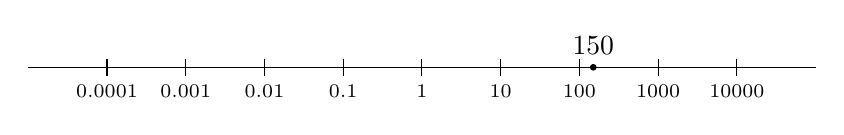
\begin{tikzpicture}
    \draw (-5,0) -- (5,0);
    \def\drawhorizontalmark#1#2{\draw (#1, 3pt) -- (#1,-3pt) node
      [below] {$\scriptstyle#2$};}
    \drawhorizontalmark{-4}{\numprint{0.0001}}%
    \drawhorizontalmark{-3}{\numprint{0.001}}%
    \drawhorizontalmark{-2}{\numprint{0.01}}%
    \drawhorizontalmark{-1}{\numprint{0.1}}%
    \drawhorizontalmark{0}{\numprint{1}}
    \drawhorizontalmark{1}{\numprint{10}}%
    \drawhorizontalmark{2}{\numprint{100}}
    \drawhorizontalmark{3}{\numprint{1000}}%
    \drawhorizontalmark{4}{\numprint{10000}}%
    \draw[fill](2.17609126, 0) circle (1pt) node [above=+1pt] {$150$};
  \end{tikzpicture}
\end{center}
ce qu'on comprend en \og prenant le logarithme (en base $10$) de tout
cela~:\fg{}
\begin{center}
  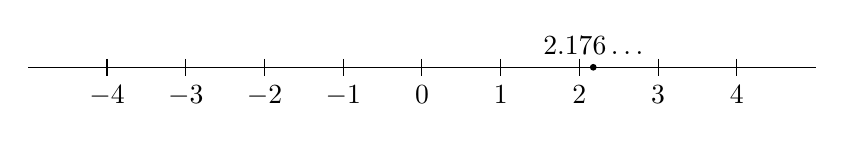
\begin{tikzpicture}
    \draw (-5,0) -- (5,0);
    \def\drawhorizontalmark#1#2{\draw (#1, 3pt) -- (#1,-3pt) node
      [below] {$#2$};}
\foreach \x in {-4, ..., 4} \drawhorizontalmark{\x}{\x};
\draw[fill] (2.17609126, 0) circle (1pt) node [above=+1pt] {$\numprint{2.176}\dots$};
  \end{tikzpicture}
\end{center}
Cette seconde droite graduée est liée à la première de la manière suivante :
\begin{center}
$10^{-4}$ = \numprint{0.0001}, $10^{-3}$ = \numprint{0.001}, \dots, $10^{3}$ = \numprint{1000}, $10^{4}$ = \numprint{10000},
\end{center}
et bien évidemment : $10^{\numprint{2.176}} = 150$.
% \mycomment{26.64\\
%   27.73\\
%   26.02\\
%   28.16\\
%   27.78\\
%   27.58\\
%   27.85\\
%   27.19}
\end{frame}
\begin{frame}{Arcsinus}
La fonction $\sin : \intercc{-\dfrac{\pi}{2}, \dfrac{\pi}{2}} \to \intercc*{-1,1}$
possède une réciproque notée :
\begin{equation*}
\arcsin : \intercc*{-1,1} \to \intercc*{-\dfrac{\pi}{2},\dfrac{\pi}{2}}
\end{equation*}

\begin{figure}[ht!]
\centering
\includegraphics[width=\textwidth]{sin-arcsin.pdf}
\caption{Graphes de $\sin$ et $\arcsin$}
\end{figure}
\end{frame}
\subsection{Fonctions trigonométriques réciproques}
\begin{frame}{Réciproque}
  \begin{definition}
    Une fonction $f\colon A \vers B$ est \Defn{inversible} si il existe une fonction $g\colon B \vers A$ telle que
    \begin{equation*}
      g(f(x)) = x\quad \forall x \in A \qquad\text{et}\qquad f(g(y)) = y \quad\forall y  \in B.
    \end{equation*}
    La fonction $g$ est appelée l'\Defn{inverse} ou la \Defn{fonction réciproque} de $f$, et se note $f^{-1}$.
  \end{definition}\pause

\begin{remark*}
  Attention à ne pas confondre $f^{-1} (x)$ avec $f(x)^{-1} \pardef 1/f(x)$~! Par exemple, les fonctions
  \begin{equation*}
    f : \RR_0 \vers \RR_0 : x\mapsto x \quad\text{et}\quad g : \RR_0 \vers
    \RR_0 : x \mapsto \frac1x
  \end{equation*}
  vérifient $f(x)^{-1} = g(x)$ pour tout $x \in \RR_0$, par contre
  $f^{-1} = f$ et $g^{-1} = g$ (exercice facile).
\end{remark*}
\end{frame}
\begin{frame}
\begin{proposition}
  \begin{enumerate}
  \item Une fonction est inversible si et seulement si c'est une bijection.
  \item Si $g$ est l'inverse de $f$, alors $f$ est l'inverse de $g$. En d'autres termes,
    \begin{equation*}
      {\left(f^{-1}\right)}^{-1} = f.
    \end{equation*}
  \end{enumerate}
\end{proposition}
\begin{proof}
  Si \(f\) est inversible (d'inverse \(g\))\pause, alors \(f\) est
  \begin{itemize}[<+->]
  \item injective car \(f(x) = f(y)\) implique \(x = g(f(x)) = g(f(y)) = y\).
  \item surjective car si \(z \in B\), alors \(g(z)\) est un antécédent de z.
  \end{itemize}\pause
  Si \(f\) est bijective, alors pour tout \(z\in B\) il existe un (surjectivité) unique (injectivité) antécédent.
\end{proof}
\end{frame}
\begin{frame}{Graphe de la réciproque}

Si $f : A \to B$ est bijective, alors le graphe de sa réciproque $f^{-1} : B \to A$ peut s'obtenir en prenant l'image du graphe de $f$ par une symétrie bilatérale d'axe $x = y$. En effet,
\begin{equation*}
\Gamma_{f^{-1}} = \{(y,f^{-1}(y)) \in \RR^2 \telque y \in B\}
= \{(f(x),x) \in \RR^2 \telque x \in A\}
\end{equation*} 
\end{frame}
\begin{frame}{Arcsinus}
La fonction $\sin : \intercc*{-\dfrac{\pi}{2}, \dfrac{\pi}{2}} \to \intercc*{-1,1}$
possède une réciproque notée :
\begin{equation*}
\arcsin : \intercc*{-1,1} \to \intercc*{-\dfrac{\pi}{2},\dfrac{\pi}{2}}
\end{equation*}

\begin{center}
\includegraphics[width=\textwidth]{sin-arcsin.pdf}
\end{center}

\end{frame}
\begin{frame}{Arccosinus}
La réciproque de $\cos : \intercc*{0,\pi} \to \intercc*{-1,1}$ est
\begin{equation*}
\arccos : \intercc*{-1,1} \to \intercc*{0,\pi}
\end{equation*}

\begin{center}
\includegraphics[width=\textwidth]{cos-arccos.pdf}
\end{center}

\end{frame}
\begin{frame}{Arctangente}
La réciproque de $\tg : \interoo*{-\dfrac{\pi}{2}, \dfrac{\pi}{2}} \to \interoo*{-\infty,
\infty}$ est 
\begin{equation*}
\arctg : \interoo*{-\infty, \infty} \to \interoo*{-\dfrac{\pi}{2},\dfrac{\pi}{2}}
\end{equation*}

\begin{center}
\includegraphics[width=\textwidth]{tan-arctan.pdf}
\end{center}

On peut aussi définir la réciproque de $\cotg : \interoo*{0,\pi} \to \interoo*{-\infty,\infty}$.
\end{frame}

\begin{frame}{Diagrammes de Venn}
Si  \(A\) et \(B\) sont des ensembles, on définit les trois opérations :
  \begin{description}
  \item[Intersection] $A \cap B = \set{ x \telque \text{\(x \in A\) et \(x \in B\)}}$
  \item[Union] $A \cup B = \set{ x \telque \text{\(x \in A\) ou \(x \in B\)}}$
  \item[Différence] $A \setminus B = \set{ x \telque \text{\(x \in A\) et \(x \notin B\)}}$
  \end{description}\pause

On peut représenter les opérations sur des diagrammes appelés diagrames de Venn.
\end{frame}

\begin{frame}
  \begin{exercise}
    Voici deux diagrammes de Venn :
    \begin{center}
      \raisebox{-.5\height}{\begin{venndiagram2sets}[shade=red] \fillACapB
        \end{venndiagram2sets}} \raisebox{-.5\height}{\begin{venndiagram3sets}[shade=green] \fillOnlyA
        \end{venndiagram3sets}}
    \end{center}
    Que représentent-ils ?
  \end{exercise}\pause

  Réponse : \(A \cap B\) et \(A\setminus (B\cup C)\)
\end{frame}

\section{Questions d'examen potentielles}
\begin{frame}
\begin{itemize}
\item Prouver (telle formule) par récurrence.
\item Qu'est ce que la transitivité (pour les inégalités) ?
\item Démontrer : si \(a < b\) et \(c < d\), alors \(a + c < b + d\).
\item Écrire \(\interco{-2,4}\cup \interoc{-5,1}\) sous forme d'intervalle.
\item Définir : l'intérieur d'un ensemble.
\item Les ensembles suivants sont ils ouverts ? fermés ? (suivi d'une liste d'ensembles)
\item De combien de manière peut on disposer \(k\) billes identiques dans deux urnes ?
\item Définir : racine carrée de \(x\).
\item Définir : fonction croissante (donner un exemple et un contre-exemple)
\item Définir le logarithme d'un nombre \(a\) en base \(b\). À quelles conditions sur \(a\) et \(b\) ce logarithme existe-t-il ?
\item Donner et prouver la formule donnant le cosinus d'une somme.
\item Donner et prouver la formule de Cauchy-Schwarz.
\item etc.
\end{itemize}
\end{frame}

% \section{Exercices}
% \begin{frame}
% \begin{itemize}
% \item Quelle est l'équation de la droite du plan qui passe par $(2,-3)$ et qui 
% est parall\`ele \`a la droite passant par $(4,1)$ et $(-2,2)$ ?
% \item \(\arccos(\frac{\sqrt{3}}{2})\), \(\arcsin(\frac{\sqrt{3}}{2})\), \(\arctan(1)\)
% \item \(\cos(\arcsin(x))\)
% \item Quelle est l'équation de la perpendiculaire \`a la droite d'équation 
% $2x-3y-4=0$, qui passe par le point $(3,-2)$ ?
% \item Pour quelles valeurs du nombre naturel $m$ avons-nous
% $
% \left(\frac{1}{2}\right)^m < 10^{-5} \quad ?
% $
% \item (difficile) Quel est le nombre de solutions enti\`eres $(x_1,x_2,\ldots, x_n)$ de l'équation $x_1+x_2+\cdots +x_n=m$, o\`u de plus $x_i>0$ pour $i=1,2,\ldots n$~?
% Ici $m$ est un naturel donné.
% \item En sommant les nombres sur les premières lignes du triangle de Pascal, intuitez la valeur de \(\sum_{k=0}^{n} \binom{n}{k}\) pour tout \(n\) fixé. Démontrez cela en utilisant le binôme de Newton pour \((1+1)^n\).
% \item Trouver les équations des droites tangentes au cercle d'équation 
% $x^2+y^2-4x-2y-3=0$ et parall\`eles \`a la droite d'équation $x+y=0$.
% \end{itemize}
% \end{frame}
% \section{Réponses}
% \begin{frame}
%   \begin{enonce}
%     En sommant les nombres sur les premières lignes du triangle de Pascal, intuitez la valeur de \(\sum_{k=0}^{n} \binom{n}{k}\) pour tout \(n\) fixé. Démontrez cela en utilisant le binôme de Newton pour \((1+1)^n\).
%   \end{enonce}

%   \begin{answer}
%     \begin{minipage}{0.49\linewidth}
%     \fbox{\includegraphics[width=.8\linewidth]{pascal2}} % triangle isocèle
%   \end{minipage}
%   \begin{minipage}{0.49\linewidth}
%   \begin{align*}
%     2^{n}  &= (1+1)^{n}\\
%            &=   \sum_{k=0}^{n} \binom{n}{k} 1^{k} 1^{n-k} \\
%     &= \sum_{k=0}^{n} \binom{n}{k}
%   \end{align*}
% \end{minipage}
% \end{answer}
% \end{frame}
% \begin{frame}
%   \begin{enonce}
%   (difficile) Quel est le nombre de solutions enti\`eres $(x_1,x_2,\ldots, x_n)$ de l'équation $x_1+x_2+\cdots +x_n=m$, o\`u de plus $x_i>0$ pour $i=1,2,\ldots n$~? Ici $m$ est un naturel donné.
% \end{enonce}

% \begin{answer}
% On place \(m\) billes et on se demande où il faut les \og séparer\fg{}. On a \(\binom{m-1}{n-1}\) choix pour les séparations.
% \end{answer}
% \end{frame}
% \begin{frame}
%   \begin{enonce}
%   Pour quelles valeurs du nombre naturel $m$ avons-nous $\left(\frac{1}{2}\right)^m < 10^{-5}$ ?
% \end{enonce}

% \begin{answer}
%  On veut \(2^{m} > 10^{5}\). Ok pour \(m \geq 17\) .
% \end{answer}
% \end{frame}
% \begin{frame}
%   \begin{enonce}
%   Quelle est l'équation de la perpendiculaire \`a la droite d'équation $2x-3y-4=0$, qui passe par le point $(3,-2)$ ?
% \end{enonce}

% \begin{answer}
% Réponse : \(3(x-3) + 2(y+2) = 0\)
% \end{answer}
% \end{frame}
% \begin{frame}
%   \begin{enonce}
% \(\cos(\arcsin(x))\)
% \end{enonce}
% \begin{answer}
% $\arcsin$ prend ses valeurs dans \(\intercc{-\pi/2, \pi/2}\). Le cosinus y est toujours positif, dès lors
% \begin{equation*}
%   \cos(\arcsin(x)) = \sqrt{1 - \sin^{2}(\arcsin(x))} = \sqrt{1 - x^{2}}
% \end{equation*}
% pour \(x \in \intercc{-1,1}\)
% \end{answer}
% \end{frame}
% \begin{frame}
%   \begin{enonce}
%     \(\arctan(1)\)
%   \end{enonce}

%   \begin{answer}
% \(\pi/4\)
% \end{answer}
% \end{frame}
% \begin{frame}
%   \begin{enonce}
% \(\arcsin(\frac{\sqrt{3}}{2})\)
% \end{enonce}

% \begin{answer}
% \(\pi/3\)
% \end{answer}
% \end{frame}
% \begin{frame}
%   \begin{enonce}
%     \(\arccos(\frac{\sqrt{3}}{2})\)
%   \end{enonce}

%   \begin{answer}
%  \(\pi/6\)
% \end{answer}

% \end{frame}
% \begin{frame}
%   \begin{enonce}
% Quelle est l'équation de la droite du plan qui passe par $(2,-3)$ et qui est parall\`ele \`a la droite passant par $(4,1)$ et $(-2,2)$ ?
% \end{enonce}

% \begin{answer}
% Vecteur directeur : \((4,1)- (-2,2) = (6,-1)\). Vecteur normal : \((1,6)\). Équation
% \begin{equation*}
%   (x-2) + 6 (y+3) = 0
% \end{equation*}
% \end{answer}
% \end{frame}
% \begin{frame}
%   \begin{enonce}
% Trouver les équations des droites tangentes au cercle d'équation $x^2+y^2-4x-2y-3=0$ et parall\`eles \`a la droite d'équation $x+y=0$.
% \end{enonce}

% \begin{answer}
% le cercle a pour équation \((x-2)^{2} + (y - 1)^{2} = 8\). Le rayon est perpendiculaire à la tangente, donc le rayon va du centre \((2,1)\) à \((2,1) \pm 2 \sqrt{2} (\sqrt{2}/2,\sqrt{2}/2) = (2,1) \pm (2,2)\) càd \((4,3)\) et \((0,-1)\). Les équations sont donc :

% \((x-4) + (y - 3) = 0\)

% \(x + y + 1 = 0\)
% \end{answer}
% \end{frame}


% \course{7}
\end{document}

%%
\section{Fonctions réelles}
\begin{frame}
  \frametitle{Motivation}
  \begin{example}
    \begin{minipage}{0.49\linewidth}
      Voici quelques fonctions de \(\RR\) dans \(\RR\), qui à \(x\) associent :
      \begin{itemize}[<+->]
      \item \(1\)
      \item \(x^{2}\)
      \item \(\exp{x}\)
      \item \(0\) si \(x < 0\), \(x^{3}\) sinon.
      \item \(\abs{x}\)
      \item \(1\) si \(x \in \QQ\) et \(0\) sinon.
      \end{itemize}\pause
      et voici les graphes de ces fonctions (sauf la dernière.)
    \end{minipage}\pause
    \begin{minipage}{0.49\linewidth}
      \begin{center}
        \includegraphics[width=4.3cm]{graphes-de-fctsreelles}
      \end{center}
    \end{minipage}
  \end{example}
\end{frame}
\begin{frame}
  \frametitle{Motivation, suite}
  Certaines fonctions sont plus agréables que d'autres.
  \begin{itemize}[<+->]
  \item Comment les caractériser ?
  \item Comment les trouver ?
  \item Quelles sont leurs propriétés ?
  \end{itemize}\pause
  Nous décrirons plusieurs classes de fonctions \og agréables\fg{} :
  \begin{itemize}[<+->]
  \item continue
  \item dérivable
  \item \(\Cclass^{\infty}\) (lire \og C infinie\fg{})
  \end{itemize}
\end{frame}

\section{Limites}

\begin{frame}{Distances}
  \begin{rappel}
    La distance entre deux réels quelconques $x$ et $y$ est $|x - y|$.
  \end{rappel}

  \begin{block}{}
  Si $\delta > 0$, demander $|x - y| < \delta$ revient donc à demander que la distance entre $x$ et $y$ soit inférieure à $\delta$.
\end{block}

\begin{block}{}
On a les équivalences suivantes~:
  \begin{equation*}
    |x - y| < \delta \iff x \in \interoo*{y-\delta,y+\delta} \iff y - \delta < x < y+\delta
  \end{equation*}
\end{block}

\end{frame}

\begin{frame}{Points adhérents}
  \begin{definition}
    Un réel $a$ est dit \Defn{adhérent} à un sous-ensemble $A$ de $\R$ si pour tout $\delta > 0$ il existe un point $x$ de $A$ tel que $|x - a| < \delta$.

    \pause On écrit aussi :
    \begin{equation}
      \forall \delta > 0, \exists x \in A : \abs{x-a} < \delta
    \end{equation}
  \end{definition}\pause

On note \(\adh A\) l'ensemble des points adhérents à \(A\).
\end{frame}

\begin{frame}
  \begin{example}
    Les points adhérents à l'ensemble ... forment l'ensemble ... :
    \begin{equation*}
      \begin{array}{cc}
        \interoc{0,1} &\intercc{0,1}\\
        \interco{0,1} &\intercc{0,1}\\
        \intercc{0,1} &\intercc{0,1}\\
        \interoo{0,1} &\intercc{0,1}\\
        \RR & \RR\\
        \interoo{-\infty, 2} &       \interoc{-\infty, 2}\\
        \RR_0 & \RR\\
        \QQ & \RR\\
        \NN &\NN
      \end{array}
  \end{equation*}
  \end{example}
\end{frame}

\begin{frame}{Idée de limite}
  Considérons la fonction \(f: \RR_0 \to \RR : x \mapsto \frac{\sin x}{x}\). \pause Son graphe~:
  \begin{center}
    \includegraphics{sinxsurx}
  \end{center}\pause
  La valeur \(f(0)\) n'a aucun sens car \(0\) n'est pas dans le domaine, car \(\frac{0}{0}\) n'a aucun sens.

  \pause Mais on a envie de dire \(f(0) = 1\).

  \pause À la place, on dira \(\limite x 0 f(x) = 1\), et on va définir cela rigoureusement.
\end{frame}

\begin{frame}{Idée de limite}
  Considérons la fonction \(f: \RR_0 \to \RR : x \mapsto \sin(1/x)\). \pause Son graphe~:
  \begin{center}
    \includegraphics{sin1surx}
  \end{center}\pause
  La valeur \(f(0)\) n'a aucun sens car \(0\) n'est pas dans le domaine, car \(\frac{1}{0}\) n'a aucun sens.

  \pause Quelle valeur a-t-on envie que \(f(0)\) prenne ? Hmm...

  \pause À la place, on dira \(\limite x 0 f(x)\) n'existe pas.
\end{frame}
  

% \begin{frame}{Idée de limite, 2}
%   Considérons la fonction \(f : \RR\)

%   Son graphe, on se l'imagine comme suit (en bleu)~:
%   \begin{center}
%     \includegraphics{graphe-de-fct-car-de-Q}
%   \end{center}

%   où les deux lignes ne sont pas continues, mais \og trouées\fg{} :
%   \begin{itemize}
%   \item les points d'abcisse rationnelle sont en haut,
%   \item ceux d'abcisse irrationnelles sont à hauteur \(0\).
% \end{itemize}

%   Donc : quand on s'approche d'une valeur fixée de \(x\), on va de haut en bas perpétuellemet
% \end{frame}


\begin{frame}{Définition de limite}
  \begin{definition}
    Soit $f : A \to B$ où $A, B \subseteq \mathbb R$ et soit $a$ un point adhérent à $A$.\pause

    Un nombre réel $L$ est la \Defn{limite de $f$ en $a$} si
    \begin{equation*}
      \forall \epsilon > 0, \exists \delta > 0 : \forall x \in A, \abs{x-a} < \delta \Rightarrow \abs{f(x)-L} < \epsilon.
    \end{equation*}
  \end{definition}\pause

  Si $L$ est la limite de $f$ en $a$, on écrit
  \begin{equation}
    \lim_{x \to a} f(x) = L.
  \end{equation}
  On dit aussi que la limite (de \(f\) en \(a\)) existe et vaut \(L\).\pause

  \begin{definition}
    S'il n'existe pas de $L \in \R$ tel que $L$ est la limite de $f$ en $a$ est $L$, on dit que la limite de $f$ en $a$ n'existe pas (dans $\R$).
  \end{definition}
\end{frame}
 
\begin{frame}
  \begin{definition}
    Ré-écrivons la définition
    \begin{equation*}
      \forall \epsilon > 0, \exists \delta > 0 : \forall x \in A, \abs{x-a} < \delta \Rightarrow \abs{f(x)-L} < \epsilon.
    \end{equation*}
  \end{definition}\pause

  \begin{remark}
    L'ordre des quantificateurs \og pour tout\fg{} et \og il existe\fg{} est importante. On choisit d'\emph{abord} une précision $\epsilon$ et puis \emph{ensuite} un rayon $\delta$ adapté à cette précision. Typiquement, au plus la précision $\epsilon$ est petite, au plus il faudra choisir le rayon $\delta$ petit.
  \end{remark}
\end{frame}

\begin{frame}{Exemple}
    Montrons que
    \begin{equation*}
      \lim_{x \to 0} \sqrt{x} = 0
    \end{equation*}
    en utilisant la définition.

    \begin{question}
      Comment doit-on choisir $\delta = \delta(\epsilon)$ pour que $|x - 0| < \delta$ (et \(x \geq 0\)) garantisse $|\sqrt{x}-0| < \epsilon$~?
    \end{question}
    \begin{answer}
      Il suffit de prendre $\delta = \epsilon^2$, car
      \begin{equation*}
        |x - 0| < \epsilon^2 \Longrightarrow 
        x < \epsilon^2 \Longrightarrow
        \sqrt{x} < \epsilon \Longrightarrow
        |\sqrt{x} - 0| < \epsilon
      \end{equation*}
      pour $x \geqslant 0$.
    \end{answer}

    Pour garantir une précision de $\epsilon = 0,01 = 10^{-2}$ on peut prendre $\delta = \epsilon^2 = 10^{-4} = 0,0001$.
\end{frame}

\begin{frame}{Unicité}
  Parler de \og la limite\fg{} n'est raisonnable que si la limite est unique.\pause \begin{proposition}Si \(L_{1}\) et \(L_{2}\) sont deux nombres vérifiant la définition de \og limite de \(f\) en \(a\), alors \(L_{1} = L_{2}\)
  \end{proposition}
\end{frame}
\begin{frame}
  \begin{proof}Supposons \(L_{1} > L_{2}\) (le cas inverse est semblable). Dès lors \(\epsilon = \paren*{L_{1} - L_{2}}/2 > 0\).

    Alors il existe \(\delta_{1} > 0\) tel que
    \begin{equation*}
      \forall x \in A, \abs{x-a} < \delta_{1} \Rightarrow \abs{f(x)-L_{1}} < \epsilon.
    \end{equation*}\pause
    et il existe \(\delta_{2} > 0\) tel que
    \begin{equation*}
      \forall x \in A, \abs{x-a} < \delta_{2} \Rightarrow \abs{f(x)-L_{2}} < \epsilon.
    \end{equation*}
    et il existe \(x \in A\) avec \(\abs{x-a} < \min\set{\delta_{1},\delta_{2}}\).

    Pour ce \(x\), on a~:
    \begin{align*}
      - (L_{1} - L_{2}) /2 &< f(x) - L_{1} &      f(x) - L_{2} &< (L_{1} - L_{2}) /2
    \end{align*}
    c'est-à-dire~:
    \begin{align*}
      (L_{1} + L_{2}) /2 < f(x) < (L_{1} + L_{2}) /2
    \end{align*}
    d'où une contradiction !
  \end{proof}
\end{frame}
\begin{frame}{Limites restreintes}
  \begin{definition}
    Si on ne s'intéresse qu'à certaines valeurs de \(x\), on écrira
    \begin{equation*}
      \limite[\text{condition sur \(x\)}] x a f(x) = L
    \end{equation*}
    lorsque
    \begin{equation*}
      \forall \epsilon > 0, \exists \delta > 0~: \forall x \in A,
      \begin{cases}
        \abs{x-a} < \delta, \text{ et}\\
        \text{condition sur \(x\)}
      \end{cases}
      \Longrightarrow \abs{f(x)-L} < \epsilon.
    \end{equation*}
    \begin{example}Les limites \og épointées\fg{}, \og à droite\fg{} et \og à gauche\fg{} sont les suivantes :
      \begin{equation*}
        \lim_{\substack{x \to a\\ x \neq a}} f(x)
        \qquad,\qquad
        \lim_{\substack{x \to a\\ x > a}} f(x)
        \qquad \textrm{et} \qquad
        \lim_{\substack{x \to a\\ x < a}} f(x)
      \end{equation*}
    \end{example}
  \end{definition}
\end{frame}

\begin{frame}{Limite épointée, limites latérales}
  \begin{example}
    La limite lorsque \(x \to 0\) de \(\abs{x}/x\) n'existe pas, mais
    \begin{align*}
      \limite [x<0] x 0 \frac{\abs{x}}{x} &= -1 &       \limite [x>0] x 0 \frac{\abs{x}}{x} &= 1
    \end{align*}

    \begin{center}
      \includegraphics{graphe-absssurx}
    \end{center}
  \end{example}
\end{frame}

\begin{frame}{Lien entre les limites}
  \begin{proposition}
    Soit \(f : A \to \RR\) et \(a \in A\). Si \(\limite{x}{a} f(x)\) existe, alors elle vaut \(f(a)\).
  \end{proposition}
  \begin{proof}\pause
    Supposons que la limite vaut \(L\) :
    \begin{equation*}
      \forall \epsilon > 0, \exists \delta > 0 : \forall x \in A, \abs{x-a} < \delta \Rightarrow \abs{f(x)-L} < \epsilon.
    \end{equation*}
    Comme \(a \in A\), on peut prendre \(x = a\). Comme \(\abs{0 - 0} < \delta\) est toujours vrai, on a forcément \(\abs{f(a) - L} < \epsilon\). Pour tout \(\epsilon > 0\) ! Donc \(f(a) = L\).
  \end{proof}\pause
  \begin{remark}
    La notion de limite intéressante est donc celle de limite épointée, où on enlève \(a\) du domaine.
  \end{remark}
\end{frame}
\begin{frame}{Lien entre les limites}
\begin{proposition}
    Lorsque \(a \in A\), \(\limite{x}{a} f(x)\) existe si et seulement si la limite épointée existe et vaut \(f(a)\).
  \end{proposition}\pause
  \begin{proposition}\label{limites épointées et latérales}
    $\displaystyle\lim_{\substack{x \to a\\ x \neq a}} f(x)$ existe si et seulement si $\displaystyle\lim_{\substack{x \to a\\ x > a}} f(x)$ et $\displaystyle\lim_{\substack{x \to a\\ x < a}} f(x)$ existent et sont \emph{égales}.
  \end{proposition}
\end{frame}

\section{Limites infinies, limites à l'infini}
\begin{frame}
  \begin{minipage}{0.49\linewidth}
 Parfois on voudrait
 \begin{itemize}
 \item écrire \(L = \pm \infty\)
 \item étudier les cas \(a = \pm \infty\)
 \end{itemize}
 \begin{remark}<2->
   La définition de limite est essentiellement :
   \begin{center}
     Si $x \approx a$ alors \(f(x)\approx L\).
   \end{center}

   Il suffira d'exprimer ces conditions différemment lorsque l'infini et impliqué.
 \end{remark}
\end{minipage}
\begin{minipage}{0.49\linewidth}
  \begin{center}
    \includegraphics{graphe-1surx}
  \end{center}
\end{minipage}
\end{frame}

\begin{frame}
  \begin{remark*}
    Chaque utilisation du symbole \(\infty\) s'accompagne d'une définition ! L'infini n'intervient pas comme un cas particulier de ce qu'on a vu précédemment.
  \end{remark*}

  \begin{definition}
    Soit \(f : A \to \RR\) une fonction réelle et \(a\) adhérent à \(A\).

    On dit que \(f(x)\) tend vers \(-\infty\) pour \(x\) tendant vers \(a\) si
    \begin{equation*}
      \forall M > 0, \exists \delta > 0 : \forall x \in A, \abs{x-a}<\delta \Rightarrow f(x) < -M
    \end{equation*}
    on note cette situation
    \begin{equation*}
      \limite x a f(x) = -\infty
    \end{equation*}
  \end{definition}
\end{frame}
\begin{frame}
  \begin{definition}
    Soit \(f : A \to \RR\) une fonction réelle dont le domaine n'est pas majoré. On dit que \(f(x)\) tend vers \(-\infty\) pour \(x\) tendant vers \(+\infty\) si
    \begin{equation*}
      \forall M > 0, \exists N > 0 : \forall x \in A, x > N \Rightarrow f(x) < -M
    \end{equation*}
    on note cette situation
    \begin{equation*}
      \limite x \infty f(x) = -\infty
    \end{equation*}
  \end{definition}
  \begin{remark}
    Les autres cas de limite infinie / à l'infini s'approchent de la même fa\c{c}on.
  \end{remark}
\end{frame}

\section{Limites et opérations}
\begin{frame}
  \begin{proposition}
    Si les deux limites, $\displaystyle{\lim_{x \to a} f(x)}$ et $\displaystyle{\lim_{x \to a} g(x)}$ existent dans $\mathbb R$, alors\pause{} $\displaystyle{\lim_{x \to a} \left[f(x)+g(x)\right]}$, $\displaystyle{\lim_{x \to a} cf(x)}$, $\displaystyle{\lim_{x \to a} \left[f(x)-g(x)\right]}$ et $\displaystyle{\lim_{x \to a} f(x)g(x)}$ existent aussi\pause{} et on a
    \begin{align*}
      \lim_{x \to a} \left[f(x)+g(x)\right] &= \lim_{x \to a} f(x) +
                                              \lim_{x \to a} g(x)\\
      \lim_{x \to a} cf(x) &= c \lim_{x \to a} f(x), \forall c \in \R\\
      \lim_{x \to a} \left[ f(x) - g(x) \right] &= \lim_{x \to a} f(x) -
                                                  \lim_{x \to a} g(x)\\
      \lim_{x \to a} f(x) g(x) &= \lim_{x \to a} f(x) \lim_{x \to a} g(x)
    \end{align*}\pause
    Si, de plus $\displaystyle{\lim_{x \to a} g(x) \neq 0}$,\pause{} alors $\displaystyle{\lim_{x \to a} \dfrac{f(x)}{g(x)}}$ existe\pause{} et on a
    \begin{equation*}
      \lim_{x \to a} \frac{f(x)}{g(x)} = \frac{\lim_{x \to a}
          f(x)}{\lim_{x \to a} g(x)}
    \end{equation*}
  \end{proposition}
\end{frame}
\begin{frame}
  \begin{proposition}
    Enfin, si on a une fonction composée $g \circ f$ et si on sait que $\displaystyle\lim_{x \to a} f(x) = L$ et que $\displaystyle\lim_{y \to L} g(y)$ existe alors $\displaystyle\lim_{x \to a} g(f(x))$ existe et on a
    \begin{equation*}
      \lim_{x \to a} g(f(x)) = \lim_{y \to L} g(y)
    \end{equation*}
  \end{proposition}
\end{frame}
\begin{frame}
  \begin{example}
    Supposons savoir que \(\sin x/x\) tend vers \(1\) en \(0\).

    Alors
    \begin{equation*}
      \limite x 0 \frac{\sin (3x)}{x} = 3 \limite x 0 \frac{\sin (3x)}{3x} = 3 \limite t 0 \frac{\sin t}{t} = 3
    \end{equation*}
  \end{example}
  \begin{remark}
    En d'autres termes, on peut poser \(t\) = fonction de \(x\), et remplacer tous les \(x\) par des \(t\), et considérer la limite pour \(t\).
  \end{remark}
\end{frame}
\begin{frame}
  \begin{example}
    \begin{equation*}
      \limite x 1 \frac{\sin (x^{2}-1)}{(x^{2}-1)} =       \limite t 0 \frac{\sin t}{t} = 1
    \end{equation*}
  \end{example}
\end{frame}

\section{Règles étendues}
\label{sec:regles-etendues}
\begin{frame}
  \begin{proposition}
    Les règles de calcul précédentes restent valables, sans modification, si on prend $a = +\infty$ ou $a = -\infty$.
  \end{proposition}

  \begin{proposition}
    Lorsque les limites sont \(\pm\infty\), chacune des \og égalités\fg{} suivante est un résultat qui se démontre :
    \begin{align*}
      (+\infty) + (+\infty) &= +\infty\\
      (-\infty) + (-\infty) &=-\infty\\
      c \cdot (\pm \infty)&=
                            \begin{cases}
                              \pm \infty &\textrm{si } c > 0\\
                              \mp \infty &\textrm{si } c < 0 \text{ (! changement de signe.)}
                            \end{cases}\\
      \infty \cdot \infty&=\infty\\
      \infty \cdot (-\infty)&=-\infty\\
      (-\infty) \cdot (-\infty)&=\infty
    \end{align*}
  \end{proposition}
\end{frame}

\begin{frame}
  En particulier, les \og quantités\fg{} suivantes n'ont aucun sens a priori :
  \begin{equation*}
    \infty - \infty,\; 0 \cdot \infty,\; 1^{\infty},\; \infty^{0},\; \frac{0}{0} \;\textrm{et}\; \frac{\infty}{\infty}.
  \end{equation*}
  
  Ce sont des \Defn{formes indéterminées}.

  \begin{example}
    \begin{equation*}
      \limite{x}{0} \frac{x^2 + x}{x^2 - x} = \frac{0}{0}
    \end{equation*}
    On ne peut pas appliquer la règle de calcul du quotient ! Il faut écrire :
    \begin{equation*}
      \limite{x}{0} \frac{x^2 + x}{x^2 - x} = \limite{x}{0} \frac{x + 1}{x - 1} = \frac{1}{-1} = -1
    \end{equation*}
  \end{example}
\end{frame}
\begin{frame}
  \begin{example}
    \begin{equation*}
      \limite{x}{\infty} \frac{x^2 + x}{x^2 - x} = \frac{\infty+\infty}{\infty - \infty}
    \end{equation*}
    On ne peut pas appliquer la règle de calcul du quotient ! Il faut écrire :
    \begin{equation*}
      \limite{x}{\infty} \frac{1 + 1/x}{1 - 1/x} 
      = \limite{x}{\infty} \frac{1 + 0}{1 - 0} = 1
    \end{equation*}
  \end{example}
\end{frame}
\begin{frame}
  \begin{proposition}
Pour le quotient, on pourra aussi prendre les conventions suivantes~:
\begin{align*}
  \frac{L}{0^+}&=
  \begin{cases}
    + \infty &\textrm{si } L > 0\\
    - \infty &\textrm{si } L < 0
  \end{cases}&
  \frac{L}{0^-}&=
  \begin{cases}
    - \infty &\textrm{si } L > 0\\
    + \infty &\textrm{si } L < 0
  \end{cases}\\
  \frac{\pm \infty}{0^+}&=\pm \infty&
  \frac{\pm \infty}{0^-}&=\mp \infty \text{ (changement de signe !)}
\end{align*}
\end{proposition}
\begin{remark}
  Une limite qui vaut $0^+$ signifie que $f(x) \to 0$ pour \(x \to a\) \texttt{et} $f(x) \geq 0$ pour $x \approx a$.
\end{remark}\pause
\begin{definition}
  Formellement, la condition $f(x) \geq 0$ pour $x \approx a$ se définit par : il existe \(\epsilon > 0\) tel que pour tout \(x\in A\) vérifiant \(\abs{x-a} < \epsilon\) on a \(f(x) \geq 0\).
\end{definition}
\end{frame}
\course{8}
\begin{frame}
  \begin{example}
    La fonction \(x \mapsto x\) a une limite nulle en \(0\). On peut cependant être plus précis et écrire~:
    \begin{align*}
      \limite[<] x 0 x &= 0^{-} & \limite[>] x 0 x &= 0^{+}.
    \end{align*}
    ce qui montre par les règles de calculs étendues :
    \begin{align*}
      \limite[<]{x}{0} \frac{1}{x} &= \frac{1}{0^{-}} = -\infty & \limite[>]{x}{0} \frac{1}{x} &= \infty.
    \end{align*}
  
    On pouvait aussi le démontrer via la définition. Par exemple pour la limite à droite : si \(K > 0\), on prend \(\delta\) un réel inférieur à \(1/K\), et alors pour tout \(x\) vérifiant \(\abs{x} < \delta\) et \(x > 0\) on a \(\frac{1}{x} > \frac{1}{\delta} = K\).
  \end{example}
\end{frame}

\begin{frame}{Landau}
  Il arrive souvent qu'on s'intéresse à comparer des fonctions \og sur le long terme\fg{}.

\begin{example}
Deux populations de bactéries peuvent avoir le même nombre d'individus au début, mais ce nombre va-t-il rester comparable tout le temps ?
\end{example}
\begin{example}
  Si deux algorithmes pour factoriser le nombre $n$ prennent respectivement $f(n)$ et $g(n)$ secondes, comment savoir lequel est le plus rapide lorsque $n$ devient grand ?
\end{example}

Nous n'allons pas répondre à ces (vagues) questions, mais nous présentons une définition utilisable dans ce cadre.
\end{frame}

\begin{frame}{Petits et grand O}
  \begin{definition}
    Soient \(f\) et \(g\) deux fonctions. Supposons qu'il existe \(r \in \RR\) et \(c \in \RR_{0}^{+}\) tels que pour tout \(x \in \interoo{r,+\infty}\) on a
    \begin{equation*}
      x \in \dom f, x \in \dom g \text{ et } \abs{f(x)} \leq c\cdot \abs{g(x)}
    \end{equation*}
    On dit alors \og $f$ est un $O(g)$\fg{} (prononcer \og \(f\) est un grand $O$ de $g$\fg{}).
\end{definition}\pause

\begin{remark}
  Cette notion indique essentiellement que \(f/g\) reste borné. Généralement on compare une fonction \(f\) intéressante à une fonction \(g\) bien connue. On dira aussi que l'\emph{ordre de grandeur} de \(f\) est inférieur à celui de \(g\).
\end{remark}
\end{frame}
\begin{frame}
\begin{example}
  \begin{itemize}
  \item \(10x\) est \(O(x)\). En effet, si \(x > 0\), on a bien \(10x \leq c x\) (par exemple \(c = 10\) fonctionne).

  \item Inversement, \(x\) est \(O(10x)\) car \(x \leq c 10x\)

  \item \(\sin(x) + x^{2}\) est en \(O(x^{2})\) car \(\sin(x) + x^{2} \leq x^{2} + x^{2} = 2 x^{2}\) si \(x > 2\).

  \item \(x^{2}\) est \(O(x)\) mais \(x\) n'est pas \(O(x^{2})\).
\end{itemize}
\end{example}
\end{frame}
\begin{frame}
\begin{proposition}
  Considérons la limite \(\limite{x}{\infty} \abs{\frac{f(x)}{g(x)}}\).
  \begin{itemize}
  \item Si elle existe dans \(\RR\), alors \(f(x)\) est \(O(g(x))\).
  \item Si elle est infinie, alors \(f(x)\) n'est pas \(O(g(x))\).
\end{itemize}
\end{proposition}
\begin{proof}
  Si la limite existe et vaut \(L\in \RR\), on prend \(\epsilon = 1\) dans la définition de limite. Ceci assure alors l'existence d'un \(N > 0\) tel que pour tout \(x \geq N\) on ait
  \begin{equation*}
    \abs{\abs{\frac{f(x)}{g(x)}} - \abs{L}} < 1
  \end{equation*}
  Dès lors \(\abs{\frac{f(x)}{g(x)}} < \abs{L} + 1\), ce qui prouve l'affirmation en prenant \(c = \abs{L} + 1\) (et \(r = N\)).

  Dans le second cas, quel que soit \(M > 0\), on sait qu'il existe \(N > 0\) tel  que pour \(x > N\), on a \(\abs{\frac{f(x)}{g(x)}} > M\). En particulier il ne peut pas exister de \(c\) vérifiant la définition de \og grand O\fg{}.
\end{proof}
\end{frame}
\begin{frame}
  \begin{example}
    Pour tout réel \(A\) : \(A x^{n}\) est \(O(x^{k})\) si et seulement si \(n \leq k\). En d'autres termes : \(x^{n}\) est d'un ordre de grandeur inférieur à \(x^{k}\) si et seulement si \(n \leq k\).

    En effet le quotient de la proposition précédente vaut \(\abs{A x^{n-k}}\) :
    \begin{itemize}
    \item Si \(n \leq k\) alors l'exposant \(n-k\) est négatif ou nul, donc le quotient tend vers \(0\) ou \(\abs A\).
    \item Si \(n > k\), alors l'exposant est strictement positif et donc le quotient tend vers \(+\infty\).
    \end{itemize}
  \end{example}
\end{frame}

\begin{frame}
  Une définition similaire est la suivante :
  \begin{definition}
    Lorsque \(\limite{x}{\infty} \abs{\frac{f(x)}{g(x)}} = 0\), on dit alors que \(f(x)\) est \(o(g(x))\).
  \end{definition}
  \begin{remark}
    \begin{itemize}[<+->]
    \item En particulier \(f(x)\) est en \(O(g(x))\) mais ceci est plus fort.
    \item On remarque que si \(g(x)\) tend vers \(0\) et \(f(x)\) est un \(o(g(x))\), alors \(f\) tend vers \(0\) plus vite que \(g\) !
    \item Les définitions de \(o\) et \(O\) tiennent encore lorsque \(x\) tend vers \(a \in \RR\) et vers \(-\infty\). Il faut alors préciser quelle est la limite pour \(x\) !
  \end{itemize}
  \end{remark}
  \begin{example}
    \begin{itemize}[<+->]
    \item \(x^{2}\) est un \(o(x^{3})\) (pour \(x \to \infty\)),
    \item \(x^{3}\)  n'est pas un \(o(x^{2})\) (pour \(x \to \infty\)),
    \item \(x^{3}\) est un \(o(x^{2})\) (pour \(x \to 0\)),
    \item \(x^{2}\)  n'est pas un \(o(x^{3})\) (pour \(x \to 0\)).
  \end{itemize}

  \end{example}
\end{frame}

\section{Continuité}
\begin{frame}
  \begin{definition}
    Soit $f : A \to B$ une fonction réelle et $a \in A$. La fonction $f$ est \Defn{continue au point $a$} si
    \begin{equation*}
      \limite[\neq] x a f(x) = f(a)
    \end{equation*}
  \end{definition}
\begin{remark*}
  Une fonction est continue en \(a\) si son comportement près de \(a\) tend vers sa valeur en \(a\).
\end{remark*}

\begin{definition}
  $f$ est \Defn[discontinue!en un point]{discontinue au point $a$} si $f$ n'est pas continue au point $a$.
\end{definition}

\begin{definition}
  $f$ est \Defn[continue!(fonction)]{continue (sur son domaine)} si elle est continue en chaque point $a$ de son domaine.
\end{definition}

\end{frame}

\begin{frame}
\begin{example}
  Par exemple, la fonction
  \begin{equation*}
    f : \R_0 \to \R : x \mapsto \frac{1}{x}
  \end{equation*}
  est continue car $f$ est continue en chaque $a \in \R_0$.
\end{example}

\begin{definition}
Une fonction $f$ est \Defn[discontinue!(fonction)]{discontinue} si elle n'est pas continue, c'est-à-dire s'il existe au moins un point \(a\) de son domaine en lequel $f$ est discontinue.
\end{definition}
\end{frame}
\begin{frame}
  \begin{example}
    \begin{enumerate}[<+->]
    \item Les fonctions suivantes sont continues :
      \begin{itemize}
      \item $g : \R \to \R : x \mapsto x^2$, et
      \item $h : \R \to \R : x \mapsto \abs x$
      \end{itemize}
    \item La fonction
      \begin{equation*}
        i : \R \to \Z : x \mapsto \lfloor x \rfloor
      \end{equation*}
      est discontinue en $a$ pour $a \in \Z$, et continue en $a$ pour $a \in \R \setminus \Z$.

    \item Enfin, la fonction caractéristique des rationnels est discontinue \emph{en chaque point $a \in \R$}.
    \end{enumerate}
  \end{example}
\end{frame}

\subsection{Continuité et opérations}
\begin{frame}
Soient deux fonctions $f$ et $g$ continues en un point \(a\). Soit $c \in \R$ une constante. Alors
\begin{align*}
  f+g &\mbox{ est continue en } a\\
  cf &\mbox{ est continue en } a\\
  f g &\mbox{ est continue en } a
\end{align*}
Si, de plus, $g(a) \neq 0$, alors
\begin{equation*}
\frac{f}{g} \mbox{ est continue en } a.
\end{equation*}
\end{frame}

\begin{frame}
  \begin{proposition}
    Si $f : A \to B$ et $g : C \to D$, avec $A, B, C, D \subset \R$ et \(\im f \subset C\) (de sorte que la composée \(g \circ f\) a du sens), si $f$ est continue en $a$ et $g$ est continue en $f(a)$ alors
    \begin{equation*}
      g \circ f \mbox{ est continue en } a.
    \end{equation*}
  \end{proposition}

  \begin{remark*}
  Ces règles de calculs sont des conséquences directes des règles de calculs pour les limites.
\end{remark*}
\end{frame}


\subsection{Propriétés importantes des fonctions continues}
\begin{frame}
  \begin{theorem}[Théorème des bornes atteintes]
    Si $f : A \to \RR$ est continue alors pour tout \(a < b \in A\) il existe \(u,v\) deux réels dans \(\intercc{a,b}\) tels que $f(\intercc{a,b}) = \intercc{f(u), f(v)}$.
  \end{theorem}
\end{frame}
\begin{frame}
  \begin{definition}% suprémum
    Soit \(E\subset\RR\) un ensemble. On dit que \(m \in \RR\) est un majorant de \(E\) si \(m \geq e\) pour tout \(e \in E\).
  \end{definition}
  \begin{theorem}[Propriété de la borne supérieure]
    Si \(E\subset\RR\) est majoré, alors il existe un plus petit majorant noté \(\sup E\). Similairement si \(E\) est minoré, il possède un plus grand minorant noté \(\inf E\).
  \end{theorem}\pause
  
  Cette propriété est une propriété fondamentale de l'ensemble des nombres réels, que nous prenons comme axiome (admise sans preuve).\pause

\begin{example}
  Si \(A = \interco{0,1} \cup \interco{2,5}\), alors~:
  \begin{align*}
    \inf A &= 0& \sup A &= 5
  \end{align*}
\end{example}
\end{frame}

\begin{frame}{Non vu au cours}
\begin{proof}[Idée de preuve du théorème de la borne atteinte]
  Nous n'allons nous intéressons qu'au cas de la borne supérieure. Le cas de la borne inférieure s'en déduit.\pause

    Montrons d'abord que \(F \pardef f([a,b])\) est majoré. Pour \(N > 0\), considérons l'ensemble \(E_{N}\) des éléments \(x \in [a,b]\) vérifiant \(f(x) \geq N\).\pause

    Notons que les ensembles \(E_{N}\) diminuent lorsque \(N\) augmente. Si \(E_{N}\) est vide pour un certain \(N\), alors \(N\) majore \(F\). Sinon, \(E_{N}\) n'est jamais vide, et toujours minoré par \(a\) et majoré par \(b\).\pause

    Considérons alors l'ensemble \(E\) des valeurs \(\sup E_{N}\) pour \(N > 0\). Cet ensemble est minoré par \(a\). Considérons donc \(c = \inf E\).\pause

    Par construction, \(c\) est arbitrairement proche de nombres dont l'image est au delà de \(N\), pour tout \(N\). D'un autre côté par continuité, les nombres proches de \(c\) ont des images proches de \(f(c)\). Ceci fournit une contradiction.\noqed
\end{proof}
\end{frame}
\begin{frame}{Non vu au cours}
  \begin{proof}[Idée de preuve, partie 2]
    L'ensemble \(F = f([a,b])\) étant majoré, il possède un supremum, notons le \(s\).\pause

    Pour \(\epsilon > 0\), on s'intéresse maintenant aux ensembles \(E_{\epsilon}\) des \(x\) tels que \(f(x) > s - \epsilon\). Il existe toujours de tels \(x\) puisque \(s - \epsilon\) n'est pas un majorant de \(F\). Cet ensemble est toujours minoré par \(a\) et majoré par \(b\).\pause

    On s'intéresse comme précédemment à l'ensemble des nombres \(\sup E_{\epsilon}\), et plus précisément à leur infimum. Ce nombre est le nombre \(v\) recherché.\pause

    Ceci montre que \(f(v)\) est la plus grande valeur prise par \(f\) sur \([a,b]\). Similairement on peut démontrer l'existence de \(u\) tel que \(f(u)\) est la plus petite valeur. Le fait que \(f([a,b]) = [f(u), f(v)]\) suivra alors du théorème suivant (de la valeur intermédiaire).
  \end{proof}
\end{frame}
\begin{frame}
\begin{example}
  L'image de \(\intercc{0,2\pi}\) par la fonction sinus est \([-1,1]\), qu'on peut effectivement ré-écrire \([\sin(3\pi/2),\sin(\pi/2)]\).
\end{example}
\end{frame}
\begin{frame}
  Il est intuitivement clair que si le graphe d'une fonction continue \og démarre\fg{} en dessous d'une droite horizontale et se termine au dessus de cette droite, il doit croiser la droite quelque part. C'est l'objet du résultat suivant \pause:

  \begin{theorem}[Théorème de la valeur intermédiaire.]
    Soit $f \colon \intercc{a,b} \to \R$ une fonction continue. Pour tout $\gamma \in \R$ strictement compris entre $f(a)$ et $f(b)$, il existe $c\in \interoo{a,b}$ tel que $f(c) = \gamma$.
  \end{theorem}
\end{frame}

\begin{frame}{Non vu au cours}
\begin{proof}[Idée de preuve]
  Nous supposons que $f(a) < \gamma < f(b)$ : le cas $f(b) < f(a)$ se déduit d'arguments similaires.\pause

  Considérons
  \[
  S = \{ x : x\in[a,b] \ \text{et }f(x)<\gamma\}.
  \]
  Cet ensemble $S$ est non-vide puisque $a \in S$ et $S$ est majoré par $b$. Donc $S$ possède un supremum. Écrivons $c= \sup S$. Évidemment $c \in \intercc{a,b} $.\pause

  Nous démontrons que $f(c) = \gamma$ en raisonnant par l'absurde :
  \begin{itemize}[<+->]
  \item Si $f(c) < \gamma$, alors il existe un point $x$ légèrement plus grand que $c$ tel que $f(x)$ est encore plus petit que $\gamma$, ce qui contredit le fait que $c$ majore $S$.
  \item Si $f(c) > \gamma$, nous voyons qu'en fait $f(x) > \gamma$ à partir d'un point légèrement plus petit que $c$, ce qui contredit le fait que $c$ est le plus petit majorant de $S$.
  \end{itemize}
\end{proof}
\end{frame}

\begin{frame}
  \begin{proposition}
    Soit \(f\) une fonction réelle bijective définie sur un intervalle. Si \(f\) est continue en \(a\), alors sa réciproque est continue en \(f(a)\).
  \end{proposition}% Exemple vu
\end{frame}

\begin{frame}
  \begin{example}
    Voyons un exemple dont le domaine n'est pas un intervalle. Soit
    \begin{equation*}
      f : \interco{0,1}\cup \interco{2,3} : x \mapsto
      \begin{cases*}
        x & si \(x < 1\)\\
        x-1 & sinon.
      \end{cases*}
    \end{equation*}
    Alors \(f\) est continue partout, mais \(f^{-1}\) n'est pas continue au point \(1\). Ci-dessous, la fonction \(f\) et la fonction \(f^{-1}\) sont représentées :
    \begin{center}
      \includegraphics{fctcontinuedinversenoncontinue}
      \quad
      \includegraphics{fctnoncontinuedinversecontinue}
    \end{center}
  \end{example}
\end{frame}
\section{Dérivées}
\begin{frame}
  \begin{rappel}
    Considérons la droite $D$ du plan passant par les points $(x,y)$ et $(x+\Delta x,y+\Delta y)$, avec \(\Delta x \neq 0\). Cette droite possède une pente
    \begin{equation*}
      m \pardef \frac{\Delta y}{\Delta x}
    \end{equation*}
    qui vaut, lorsque le repère est orthonormé, la tengente de l'angle formé par la droite avec l'horizontale.
  \end{rappel}\pause
% \end{frame}
% \begin{frame}
  \begin{definition}
    Soit $f : A \subset \RR \to \RR$ une fonction, et soit $a$ un point intérieur à $A$. Si la limite
    \begin{equation*}
      \lim_{\substack{x \to a\\ x \neq a}} \frac{f(x)-f(a)}{x-a}
    \end{equation*}
    existe dans \(\RR\), on appelle cette limite le \Defn{nombre dérivé de $f$ en $a$} et on le note $f'(a)$.
  \end{definition}\pause

  Quand cette limite existe, on dit que $f$ est \Defn{dérivable} au point $a$, ou encore que $f'(a)$ existe.
\end{frame}
\begin{frame}
  %%Created by jPicEdt 1.4.1_03: mixed JPIC-XML/LaTeX format
%%Thu Sep 03 01:08:16 CEST 2009
%%Begin JPIC-XML
%<?xml version="1.0" standalone="yes"?>
%<jpic x-min="-2.1" x-max="88.33" y-min="-2.3" y-max="46.8" auto-bounding="true">
%<multicurve left-arrow= "head"
%	 arrow-head-length-scale= "1.5"
%	 arrow-head-width-minimum= "1.2"
%	 points= "(4.84,45.16);(4.84,45.16);(4.83,-2.3);(4.83,-2.3)"
%	 fill-style= "none"
%	 />
%<multicurve arrow-head-length-scale= "1.6"
%	 right-arrow= "head"
%	 arrow-head-width-minimum= "1.2"
%	 points= "(-2.1,4.84);(-2.1,4.84);(88.33,4.84);(88.33,4.84)"
%	 fill-style= "none"
%	 />
%<text text-vert-align= "center-v"
%	 anchor-point= "(-0.32,38.06)"
%	 fill-style= "none"
%	 text-frame= "noframe"
%	 text-hor-align= "center-h"
%	 >
%$y$
%</text>
%<text text-vert-align= "center-v"
%	 anchor-point= "(70.6,-0.08)"
%	 fill-style= "none"
%	 text-frame= "noframe"
%	 text-hor-align= "center-h"
%	 >
%$x$
%</text>
%<multicurve points= "(5.26,13.32);(5.26,13.32);(37.28,41.45);(37.28,41.45)"
%	 fill-style= "none"
%	 />
%<multicurve points= "(27.33,32.52);(27.33,32.52);(27.33,20.91);(27.33,20.91)"
%	 fill-style= "none"
%	 />
%<multicurve points= "(13.91,20.91);(13.91,20.91);(27.33,20.91);(27.33,20.91)"
%	 fill-style= "none"
%	 />
%<text text-vert-align= "center-v"
%	 anchor-point= "(30.36,25.37)"
%	 fill-style= "none"
%	 text-frame= "noframe"
%	 text-hor-align= "center-h"
%	 >
%$\Delta y$
%</text>
%<text text-vert-align= "center-v"
%	 anchor-point= "(19.97,17.78)"
%	 fill-style= "none"
%	 text-frame= "noframe"
%	 text-hor-align= "center-h"
%	 >
%$\Delta x$
%</text>
%<text text-vert-align= "center-v"
%	 anchor-point= "(26.9,35.2)"
%	 fill-style= "none"
%	 text-frame= "noframe"
%	 text-hor-align= "center-h"
%	 >
%$P_2$
%</text>
%<text text-vert-align= "center-v"
%	 anchor-point= "(10.45,22.7)"
%	 fill-style= "none"
%	 text-frame= "noframe"
%	 text-hor-align= "center-h"
%	 >
%$P_1$
%</text>
%<pscurve closed= "false"
%	 curvature= "1;0.1;0"
%	 points= "(8.72,9.75);(9.15,13.32);(33.82,34.3);(60.64,17.34);(73.19,46.8);(74.92,57.97)"
%	 fill-style= "none"
%	 />
%<text text-vert-align= "center-v"
%	 anchor-point= "(57.9,29.84)"
%	 fill-style= "none"
%	 text-frame= "noframe"
%	 text-hor-align= "center-h"
%	 >
%$y = f(x)$
%</text>
%</jpic>
%%End JPIC-XML
%LaTeX-picture environment using emulated lines and arcs
%You can rescale the whole picture (to 80% for instance) by using the command \def\JPicScale{0.8}
\ifx\JPicScale\undefined\def\JPicScale{1}\fi
\unitlength \JPicScale mm
\begin{picture}(88.33,46.8)(0,0)
\linethickness{0.3mm}
\put(4.84,-2.3){\line(0,1){47.47}}
\put(4.84,45.16){\vector(0,1){0.12}}
\linethickness{0.3mm}
\put(-2.1,4.84){\line(1,0){90.43}}
\put(88.33,4.84){\vector(1,0){0.12}}
\put(-0.32,38.06){\makebox(0,0)[cc]{$y$}}

\put(70.6,-0.08){\makebox(0,0)[cc]{$x$}}

\linethickness{0.3mm}
\multiput(5.26,13.32)(0.14,0.12){234}{\line(1,0){0.14}}
\linethickness{0.3mm}
\put(27.33,20.91){\line(0,1){11.61}}
\linethickness{0.3mm}
\put(13.91,20.91){\line(1,0){13.42}}
\put(30.36,25.37){\makebox(0,0)[cc]{$\Delta y$}}

\put(19.97,17.78){\makebox(0,0)[cc]{$\Delta x$}}

\put(26.9,35.2){\makebox(0,0)[cc]{$P_2$}}

\put(10.45,22.7){\makebox(0,0)[cc]{$P_1$}}

\linethickness{0.3mm}
\qbezier(9.15,13.32)(13.15,21.06)(19.42,27.23)
\qbezier(19.42,27.23)(25.7,33.41)(33.82,34.3)
\qbezier(33.82,34.3)(41.53,33.44)(47.48,24.9)
\qbezier(47.48,24.9)(53.44,16.36)(60.64,17.34)
\qbezier(60.64,17.34)(67.6,20.27)(69.47,29.27)
\qbezier(69.47,29.27)(71.34,38.27)(73.19,46.8)
\put(57.9,29.84){\makebox(0,0)[cc]{$y = f(x)$}}

\end{picture}

\end{frame}

\begin{frame}
  %%Created by jPicEdt 1.4.1_03: mixed JPIC-XML/LaTeX format
%%Mon Sep 14 09:20:08 CEST 2009
%%Begin JPIC-XML
%<?xml version="1.0" standalone="yes"?>
%<jpic x-min="-1.94" x-max="88.49" y-min="-2.63" y-max="47.9" auto-bounding="true">
%<multicurve arrow-head-length-scale= "1.5"
%	 arrow-head-width-minimum= "1.2"
%	 left-arrow= "head"
%	 fill-style= "none"
%	 points= "(5,47.9);(5,47.9);(4.99,-2.63);(4.99,-2.63)"
%	 />
%<multicurve arrow-head-length-scale= "1.6"
%	 arrow-head-width-minimum= "1.2"
%	 right-arrow= "head"
%	 fill-style= "none"
%	 points= "(-1.94,4.52);(-1.94,4.52);(88.49,4.52);(88.49,4.52)"
%	 />
%<text text-vert-align= "center-v"
%	 anchor-point= "(-0.65,37.9)"
%	 fill-style= "none"
%	 text-frame= "noframe"
%	 text-hor-align= "center-h"
%	 >
%$y$
%</text>
%<text text-vert-align= "center-v"
%	 anchor-point= "(70.76,-0.4)"
%	 fill-style= "none"
%	 text-frame= "noframe"
%	 text-hor-align= "center-h"
%	 >
%$x$
%</text>
%<multicurve fill-style= "none"
%	 points= "(18.83,27.73);(18.83,27.73);(38.74,38.44);(38.74,38.44)"
%	 />
%<multicurve fill-style= "none"
%	 points= "(27.49,32.19);(27.49,32.19);(27.49,30.86);(27.49,30.86)"
%	 />
%<multicurve fill-style= "none"
%	 points= "(24.89,30.86);(24.89,30.86);(27.49,30.86);(27.49,30.86)"
%	 />
%<text text-vert-align= "center-v"
%	 anchor-point= "(25.62,35.62)"
%	 fill-style= "none"
%	 text-frame= "noframe"
%	 text-hor-align= "center-h"
%	 >
%$P_2$
%</text>
%<text text-vert-align= "center-v"
%	 anchor-point= "(21.88,32.5)"
%	 fill-style= "none"
%	 text-frame= "noframe"
%	 text-hor-align= "center-h"
%	 >
%$P_1$
%</text>
%<pscurve fill-style= "none"
%	 closed= "false"
%	 curvature= "1;0.1;0"
%	 points= "(8.88,9.43);(9.31,13);(33.98,33.98);(60.8,17.02);(73.35,46.48);(75.08,57.64)"
%	 />
%<text text-vert-align= "center-v"
%	 anchor-point= "(58.06,29.52)"
%	 fill-style= "none"
%	 text-frame= "noframe"
%	 text-hor-align= "center-h"
%	 >
%$y = f(x)$
%</text>
%</jpic>
%%End JPIC-XML
%LaTeX-picture environment using emulated lines and arcs
%You can rescale the whole picture (to 80% for instance) by using the command \def\JPicScale{0.8}
\ifx\JPicScale\undefined\def\JPicScale{1}\fi
\unitlength \JPicScale mm
\begin{picture}(88.49,47.9)(0,0)
\linethickness{0.3mm}
\put(5,-2.63){\line(0,1){50.53}}
\put(5,47.9){\vector(0,1){0.12}}
\linethickness{0.3mm}
\put(-1.94,4.52){\line(1,0){90.43}}
\put(88.49,4.52){\vector(1,0){0.12}}
\put(-0.65,37.9){\makebox(0,0)[cc]{$y$}}

\put(70.76,-0.4){\makebox(0,0)[cc]{$x$}}

\linethickness{0.3mm}
\multiput(18.83,27.73)(0.22,0.12){89}{\line(1,0){0.22}}
\linethickness{0.3mm}
\put(27.49,30.86){\line(0,1){1.33}}
\linethickness{0.3mm}
\put(24.89,30.86){\line(1,0){2.6}}
\put(25.62,35.62){\makebox(0,0)[cc]{$P_2$}}

\put(21.88,32.5){\makebox(0,0)[cc]{$P_1$}}

\linethickness{0.3mm}
\qbezier(9.31,13)(13.28,20.65)(19.52,26.87)
\qbezier(19.52,26.87)(25.77,33.08)(33.98,33.98)
\qbezier(33.98,33.98)(41.73,33.12)(47.64,24.61)
\qbezier(47.64,24.61)(53.56,16.1)(60.8,17.02)
\qbezier(60.8,17.02)(67.93,19.93)(69.73,28.95)
\qbezier(69.73,28.95)(71.52,37.97)(73.35,46.48)
\put(58.06,29.52){\makebox(0,0)[cc]{$y = f(x)$}}

\end{picture}

\end{frame}
\begin{frame}
\begin{example}
  Si \(f(x) = x^{2}\), le nombre dérivé de \(f\) en \(a\) est \(2a\)
\end{example}
\begin{proof}
  On remarque que
  \begin{equation*}
\frac{f(x)-f(a)}{x-a} = \frac{x^{2}-a^{2}}{x-a} = \frac{(x-a)(x+a)}{x-a} = x+a
\end{equation*}
pour tout \(x \neq a\). Dès lors lorsque \(x \to a\), la limite vaut bien \(a + a = 2a\).
\end{proof}

On notera donc \(f'(a) = 2a\), ou \(f'(x) = 2x\).
\end{frame}
\begin{frame}
  Étant donnée \(f\) une fonction, la notion de dérivabilité ci-dessus donne lieu à une nouvelle fonction, notée \(f'\) qui à chaque valeur \(x\)  pour laquelle \(f\) est dérivable associe le nombre dérivé de \(f\) en \(x\), c'est-à-dire \(f'(x)\). Cette fonction \(f'\) est appelée la fonction dérivée de \(f\).
\end{frame}
\course{9}
\begin{frame}{Opérations sur les fonctions}
  \begin{remark}
    On sait bien ce qu'est la somme de deux nombres mais nous n'avons pas encore défini la somme, le produit, etc. de deux fonctions. Les définitions présentées ci-après ne surprendront cependant personne.
  \end{remark}

  Soit \(f\) et \(g\) deux fonctions de domaine \(A\) à valeurs dans \(\RR\), et \(c\) un nombre.
  \begin{align*}
    f+g: A \to \RR &: x \mapsto (f+g)(x) \pardef f(x) + g(x) \\
    cf: A \to \RR &: x \mapsto (cf)(x) \pardef c \cdot f(x) \\
    fg: A \to \RR &: x \mapsto (fg)(x) \pardef f(x)g(x) \\
    \uncover<2->{    f/g: \set{x \in A \telque g(x)\neq 0} \to \RR &: x \mapsto (f/g)(x) \pardef f(x)/g(x)}
  \end{align*}
\end{frame}
\begin{frame}
  \begin{proposition}Pour $a$ une constante, et $f$ et $g$ des fonctions dérivables, on a
    \begin{enumerate}
    \item $(af)' = a f'$
    \item $(f + g)' = f' + g'$
    \item $(f g)' = f' g + f g'$
    % \item $\dfrac{\mathrm{d} ((f(x))^a)}{\mathrm{d} x} = a \, f^{a-1}(x)
    %   f'(x)$ \\
    %   et en particulier~: $\left( x^a \right)' = a \, x^{a-1}$
    \item Sur un domaine où $g$ est non-nulle : $\left(\frac{f}{g}\right)' = \frac{f'g - fg'}{g^2}$.
    \end{enumerate}
  \end{proposition}
  Nous allons détailler quelques preuves.
\end{frame}
\begin{frame}
  \begin{proposition}Si \(a\) est une constante et \(f\) une fonction, alors
    \((af)'= a f'\)
  \end{proposition}
  \begin{proof}\pause
    Il faut montrer que pour tout \(u\) dans le domaine de \(f'\), \((af)'(u) = a f'(u)\).\pause
    On calcule simplement :
    \begin{align*}
      \limite{x}{u} \frac{(af)(x)-(af)(u)}{x-u} &= \limite{x}{u} \frac{a f(x) - a f(u)}{x-u}\\
                                                &= \limite{x}{u} a \frac{f(x) - f(u)}{x-u}\\
                                                &= a \limite{x}{u} \frac{f(x) - f(u)}{x-u}\\
                                                &= a f'(u)\\
    \end{align*}
  \end{proof}
\end{frame}
\begin{frame}
  \begin{proposition}
    Si \(f,g\) sont deux fonctions, alors $(f + g)' = f' + g'$
  \end{proposition}
  \begin{proof}\pause
    Vérifions l'égalité en un point \(u\) où \(f\) et \(g\) sont toutes les deux dérivables :
    \begin{align*}
      \limite{x}{u} \frac{(f+g)(x)-(f+g)(u)}{x-u} &= \limite{x}{u} \frac{f(x) + g(x) - f(u) - g(u)}{x-u}\\
                                                  &= \limite{x}{u} \frac{f(x) - f(u)}{x-u} + \frac{g(x) - g(u)}{x-u}\\
      &= f'(u) + g'(u)
    \end{align*}
    d'où le résultat.
  \end{proof}
\end{frame}
\begin{frame}
  Avant de prouver le résultat pour le produit, nous aurons besoin du résultat suivant :
  \begin{proposition}
    Si \(f\) est dérivable en \(u\), alors \(f\) est continue en \(u\).
  \end{proposition}
  \begin{proof}\pause 
    On suppose que \(\limite{x}{u} \frac{f(x)-f(u)}{x-u}\) existe et vaut un nombre réel (\(f'(u)\)). Alors pour tout \(x \neq u\) :
    \begin{equation*}
      f(x) = \frac{f(x)-f(u)}{x-u} (x-u) + f(u)
    \end{equation*}\pause
    et donc en passant à la limite~:
    \begin{equation*}
      \limite x u f(x) = \limite x u \frac{f(x)-f(u)}{x-u} (x-u) + f(u) = f'(u) 0+ f(u) = f(u).
    \end{equation*}
  \end{proof}
\end{frame}
\begin{frame}
  \begin{proposition}
    Si \(f\) et \(g\) sont des fonctions dérivables en \(u\), alors \((fg)'(u) = f'(u)g(u) + f(u) g'(u)\)
  \end{proposition}
  \begin{proof}\pause
    \begin{align*}
      \limite{x}{u} \frac{(fg)(x)-(fg)(u)}{x-u} &= \limite{x}{u} \frac{f(x)g(x) - f(u)g(u)}{x-u}\\
                                                &= \limite{x}{u} \frac{f(x)g(x) - f(x) g(u) + f(x) g(u) - f(u)g(u)}{x-u}\\
                                                &= \limite{x}{u} \frac{f(x)(g(x) - g(u)) + (f(x) - f(u))g(u)}{x-u}\\
                                                &= \limite{x}{u} \frac{f(x)(g(x) - g(u))}{x-u} + \frac{(f(x) - f(u))g(u)}{x-u}\\
                                                &= \limite{x}{u} f(x) \frac{g(x) - g(u)}{x-u} + \limite{x}{u} \frac{(f(x) - f(u))}{x-u} g(u)\\
                                                &= f(u) g'(u) + f'(u) g(u)
    \end{align*}
  \end{proof}
\end{frame}
\begin{frame}
  \begin{proposition}
    La dérivée \(1/f\) est \(-f'/f^{2}\) en tout point où \(f\) ne s'annule pas.
  \end{proposition}
  \begin{proof}\pause
    \begin{align*}
      \limite x u \frac{\frac{1}{f(x)} - \frac{1}{f(u)}}{x-u} &= \limite x u \frac{\frac{f(u) - f(x)}{f(x)f(u)}}{x-u}\\
&= \limite x u \frac{1}{f(x)f(u)} \frac{f(u)-f(x)}{x-u}\\
      &= -\frac{f'(u)}{f(u)^{2}}
    \end{align*}
  \end{proof}
  \begin{exercise}
    Démontrer \((f/g)'s = (f'g-fg')/g^{2}\) en combinant les deux dernières propositions.
  \end{exercise}
\end{frame}
\begin{frame}{Dérivées élémentaires}
  \begin{proposition}
    La dérivée de \(f\) définie par \(f(x) = x\) est la fonction \(f'\) telle que \(f'(x) = 1\).\pause

    En général, on dira simplement \og La dérivée de \(x\) est \(1\)\fg{}.\pause

    Parfois on précisera \og par rapport à \(x\)\fg{}.
  \end{proposition}
  \begin{proof}
    \begin{equation*}
    f'(u) = \limite{x}{u} \frac{x-u}{x-u} = 1
  \end{equation*}
  \end{proof}
\end{frame}
\begin{frame}
  \begin{proposition}
    La dérivée de \(x^{n}\) vaut \(n x^{n-1}\) pour tout naturel \(n\).
  \end{proposition}
  \begin{proof}
    Prouvons-le par induction. Si \(n = 1\), cela revient à prouver que la dérivée de \(x\) vaut \(1\), ce qui a déjà été fait.\pause

    Fixons \(n \geq 1\) et supposons que la dérivée de \(x^{n}\) vaut \(nx^{n-1}\) pour cette valeur fixée.\pause{} Alors:
    \begin{equation*}
      (x^{n+1})' = (x x^{n})' = (x)' x^{n} + x (x^{n})' = 1 x^{n} + x n x^{n-1} = x^{n} + n x^{n} = (n+1) x^{n}
    \end{equation*}
    ce qui est bien la formule attendue pour \(n+1\).
  \end{proof}
\end{frame}
\begin{frame}
  \begin{proposition}
    Considérons \(f(x) = a^{x}\). Alors \(f'(x) = a^{x} \ln(a)\).
  \end{proposition}
  \begin{remark*}\pause
    Les deux écritures suivantes sont identiques :
    \begin{equation*}
      \limite{x}{u} \frac{f(x)-f(u)}{x-u} = \limite{h}{0} \frac{f(u+h) - f(u)}{h}
    \end{equation*}
  \end{remark*}\pause
  \begin{proof}[Preuve incomplète]\pause
    \begin{equation*}
      (a^{x})' = \limite{h}{0} \frac{a^{x+h}-a^{x}}{h} = \limite{h}{0} a^{x} \frac{a^{h} - 1}{h} = a^{x} \limite{h}{0} \frac{a^{h}-1}{h}
    \end{equation*}
    Nous ne pouvons pas démontrer l'égalité \(\limite{h}{0} \frac{a^{h}-1}{h} = \ln(a)\) actuellement.
  \end{proof}
\end{frame}
\begin{frame}
  \begin{remark}
    Retenons que \(\exp x\) est une fonction égale à sa propre dérivée !
  \end{remark}\pause
  \begin{exercise}
    Pouvez-vous trouver d'autres fonctions qui sont égale à leur propre dérivée ? % (C'est-à-dire telles que \(f'(x) = f(x)\) pour tout \(x\) dans un certain domaine de définition.)
    % Pouvez-vous \emph{toute} les trouver ? Pas encore : il faut avoir f' = 0 => f = cste.
  \end{exercise}
  % \begin{answer}
  %   Si \(f' = f\), alors \(0 = f' \exp{-x} - \exp{-x} f = (f \exp {\paren*{-x}})'\)
  % \end{answer}
\end{frame}
\begin{frame}
  \begin{proposition}
    Si \(f\) et \(g\) sont des fonctions et \(a\) est intérieur au domaine de \(f \circ g\)\pause, si \(g\) est dérivable en \(a\) et \(f\) dérivable en \(g(a)\)\pause, alors
    \begin{equation*}
      (f\circ g)'(a) = f'(g(a)) g'(a).
    \end{equation*}
  \end{proposition}
  \begin{proof}\pause
    \begin{align*}
      \limite x a \frac{f(g(x)) - f(g(a))}{x-a}
      \uncover<+->{&= \limite x a \paren*{\frac{f(g(x)) - f(g(a))}{g(x)-g(a)}}\paren*{\frac{g(x)-g(a)}{x-a}}\\}
      \uncover<+->{&= \limite x a \frac{f(g(x)) - f(g(a))}{g(x)-g(a)} \limite x a \frac{g(x)-g(a)}{x-a}\\}
      \uncover<+->{&= \limite t {g(a)} \frac{f(t) - f(g(a))}{t-g(a)} \limite x a \frac{g(x)-g(a)}{x-a}\\}
      \uncover<+->{&= f'(g(a)) g'(a)\\}
      \uncover<+->{&\text{on a utilisé la continuité de \(g\) en \(a\) !}}
    \end{align*}\pause
  \end{proof}
  \begin{remark*}
    On a passé sous silence le fait que \(g(x)\) et \(g(a)\) pourraient être égal.
  \end{remark*}
\end{frame}
\begin{frame}
  \begin{example}
    Si \(f(x) = \exp{(nx)}\), c'est la composée de l'exponentielle et de \(x\mapsto nx\). La dérivée de l'exponentielle est elle-même, la dérivée de \(nx\) est \(n\), dès lors \(f'(x) = \exp{(nx)} n\).\pause

    Notons qu'on peut également écrire \(f(x) = (\exp{x})^{n}\), d'où on voit \(f\) comme la composée de \(t\mapsto t^{n}\) et de l'exponentielle. La dérivée de \(t^{n}\) par rapport à \(t\) est \(n t^{n-1}\), dès lors \(f'(x) = n (\exp{x})^{n-1} \exp{x} = n (\exp{x})^{n}\).\pause

    Le résultat est évidemment le même.
  \end{example}
\end{frame}
\begin{frame}
  Avant de passer à un résultat sur la dérivée des logarithmes, nous avons besoin de :
  \begin{lemma}
    Si \(f : I \to \RR\) est une injection continue définie sur un intervalle, alors \(f\) est strictement monotone (c'est-à-dire strictement croissante ou strictement décroissante).
  \end{lemma}
  \begin{proof}
    Considérons le domaine \(T\) des points \((x,y)\in I \times I\) avec \(x > y\). Ceci forme un triangle.

    \begin{center}
      \includegraphics[width=3.8cm]{triangle} 
    \end{center}
  \end{proof}
\end{frame}
\begin{frame}
  \begin{proof}
    Supposons qu'il existe \((x,y)\) dans \(T\) et \((u,v)\) dans \(T\) avec \(f(x)-f(y)\) positif et \(f(u)-f(v)\) négatif.\pause{} Considérons alors le point
    \begin{equation*}
      \point{p}(t) = (p_{1}(t), p_{2}(t)) = (x,y) + t((u,v)-(x,y)).
    \end{equation*}\pause
    Lorsque \(t\) varie, ce point va du point \((x,y)\) au point \((u,v)\) en ligne droite, et donc en restant dans le triangle \(T\).\pause{} La quantité \(f(p_{1}(t))-f(p_{2}(t))\) est\pause
    \begin{itemize}
    \item positive en \(t = 0\) (correspondant au point \((x,y)\)) et\pause
    \item négative en \(t = 1\).
    \end{itemize}\pause
    Dès lors, par continuité, elle s'annule pour une certaine valeur de \(t\)\pause, c'est-à-dire il existe \(t\) tel que
    \begin{equation*}
      f(p_{1}(t)) = f(p_{2}(t))
    \end{equation*}
    Comme \(f\) est injective, cela implique \(p_{1}(t) = p_{2}(t)\). Mais ceci n'est pas possible car le point \(\point{p}(t)\) est dans \(T\) et donc \(p_{1}(t) > p_{2}(t)\) !
  \end{proof}
\end{frame}
\begin{frame}
  \begin{proposition}
    Si \(f : A \to B\) est une bijection dérivable en \(a\) avec \(f'(a)\neq 0\), alors sa réciproque \(f^{-1}\) est dérivable en \(f(a)\) et
    \begin{equation*}
      (f^{-1})'(f(a)) = \frac{1}{f'(a)}.
    \end{equation*}
  \end{proposition}
  \begin{proof}\pause
    % Comme \(f'(a)\neq 0\), on sait
    % \begin{math}
    %   \limite x a \frac{x-a}{f(x)-f(a)} = \frac{1}{f'(a)}
    % \end{math}\pause
    Comme \(f\) est une bijection dérivable en \(a\), elle est également continue en \(a\) et son inverse est donc continue en \(f(a)\).\pause{} Dès lors nous avons
    \begin{math}
      \limite{t}{f(a)} f^{-1}(t) = f^{-1}(f(a)) = a.
    \end{math}\pause
    On a donc successivement
    \begin{align*}
      \frac{1}{f'(a)} &= \limite x a \frac{x-a}{f(x)-f(a)} = \limite x a \frac{f^{-1}(f(x)) - f^{-1}(f(a))}{f(x)-f(a)} \\
      &= \limite t f(a) \frac{f^{-1}(t) - f^{-1}(f(a))}{t-f(a)}
    \end{align*}\pause
    où la dernière égalité s'obtient par la règle de composition des limites.\pause{} Ceci est la définition du nombre dérivé de \(f^{-1}\) en \(f(a)\).
  \end{proof}
\end{frame}

\begin{frame}
  \begin{example}
    La dérivée de \(\ln(x)\) vaut \(1/x\).
  \end{example}
  \begin{proof}
    On sait que \(\ln\) est la réciproque de \(\exp\), dès lors
    \begin{equation*}
      \ln'(x) = \frac{1}{\exp'{\ln(x)}} = \frac{1}{\exp{\paren*{\ln x}}} = \frac{1}{x}.
    \end{equation*}
  \end{proof}
  \begin{example}
    La fonction \(f : \RR_0 \to \RR : x \mapsto \ln\abs{x}\) a pour dérivée \(\frac{1}{x}\).
  \end{example}
  \begin{proof}
    \begin{itemize}
    \item Pour \(x > 0\), c'est simplement \(\ln x\) ;\pause
    \item pour \(x < 0\), c'est \(\ln (-x)\), \pause{} dont la dérivée vaut \(\frac{1}{-x} (-x)' = \frac{1}{x}\) également par la règle sur la dérivée d'une composée.
    \end{itemize}
  \end{proof}
\end{frame}
\begin{frame}
  \begin{proposition}
    La dérivée de \(x^{n}\) vaut \(n x^{n-1}\) pour tout réel \(n\), \(x > 0\).
  \end{proposition}
  \begin{example}
    \begin{itemize}[<+->]
    \item Nous savons que c'est vrai pour \(n\) naturel.
    \item Pour \(n = 1/2\), nous observons~:
      \begin{align*}
        \limite{h}{0} \frac{\sqrt{x+h}-\sqrt{x}}{h} 
        & = \limite{h}{0} \frac{(\sqrt{x+h}-\sqrt{x})(\sqrt{x+h}+\sqrt{x})}{h(\sqrt{x+h}+\sqrt{x})} \\
        &= \limite{h}{0} \frac{h}{h(\sqrt{x+h}+\sqrt{x})} = \frac{1}{2\sqrt{x}} = \frac{1}{2} x^{-1/2}
      \end{align*}
    \item Pour \(n = 1/3\), nous observons~:
      \begin{align*}
        &\limite{h}{0} \frac{\sqrt[3]{x+h}-\sqrt[3]{x}}{h} 
        = \limite{h}{0} \frac
          {(\sqrt[3]{x+h}-\sqrt[3]{x})(\sqrt[3]{x+h}^{2}+\sqrt[3]{x+h}\sqrt[3]{x}+\sqrt[3]{x}^{2})}
          {h(\sqrt[3]{x+h}^{2}+\sqrt[3]{x+h}\sqrt[3]{x}+\sqrt[3]{x}^{2})}\\
        &= \limite{h}{0} \frac{h}{h(\sqrt[3]{x+h}^{2}+\sqrt[3]{x+h}\sqrt[3]{x}+\sqrt[3]{x}^{2})} = \frac{1}{3\sqrt[3]{x}^{2}} = \frac{1}{3} x^{-2/3}
      \end{align*}
    \end{itemize}
  \end{example}
\end{frame}
\begin{frame}
\begin{proof}\pause
    \begin{equation*}
      x^n = \exp{\paren*{\ln(x^n)}} = \exp{\paren*{n \ln(x)}}
    \end{equation*}
    En dérivant cette dernière expression nous obtenons le résultat.
  \end{proof}
\end{frame}

\subsection{Dérivée seconde, troisième, etc\ldots}
\begin{frame}{Questions de notations}
  Dans vos cours vous rencontrerez les notations suivantes pour la dérivée d'une fonction \(f\) en un point \(a\) :
\begin{itemize}[<+->]
\item \(f'(a)\)
\item \(\dfrac{\D f}{\D x}(a)\)
\end{itemize}\pause
Ou, ayant écrit \(y = f(x)\) :
\begin{itemize}[<+->]
\item \(y'(a)\)
\item \(\dfrac{\D y}{\D x}(a)\)
\end{itemize}
\end{frame}

\begin{frame}
  Supposons\pause
  \begin{itemize}[<+->]
  \item $f$ est dérivable dans un intervalle ouvert $\interoo{a,b}$, et
  \item si sa dérivée $f'$ est aussi dérivable dans $\interoo{a,b}$,
  \end{itemize}\pause
  alors on définit la \Defn{dérivée seconde}, notée $f''$ par :
  \begin{equation*}
    f''(x) = (f')'(x); \qquad x \in \interoo{a,b}
  \end{equation*}\pause
  
  Si $f''$ admet à son tour une dérivée dans $\interoo{a,b}$, on l'appelle \Defn{dérivée troisième}, notée $f'''$ ou $f^{\underline{3}}$ et ainsi de suite, c'est-à-dire
  \begin{equation*}
    f^{\underline{(n+1)}}=(f^{\underline{n}})'
  \end{equation*}
  récursivement, pour tout \(n\).
\end{frame}

\course{10}
\section{Étude de fonction}
\subsection{Croissance et décroissance}
\begin{frame}
  Nous avons introduit le nombre dérivé comme la pente de la tengente (géométrique) au graphe de la fonction.\pause
  
  Intuitivement,
  \begin{itemize}\pause
  \item si la dérivée est positive, la fonction doit donc \og monter\fg{} (être localement croissante),\pause
  \item si la dérivée est négative, la fonction doit donc \og descendre\fg{}.
  \end{itemize}\pause

  Nous allons \uncover<+->{(plus ou moins)} démontrer ce résultat.
\end{frame}
\begin{frame}
  \begin{definition}\label{extremum}
    Soit \(f\) une fonction réelle et \(a\) un point de son domaine. Ce point est
    \begin{itemize}[<+->]
    \item un \Defn{minimum} (global) de \(f\) si \(f(a) \leq f(x)\) pour tout \(x \in \dom f\) ;
    \item un \Defn{maximum} (global) de \(f\) si \(f(a) \geq f(x)\) pour tout \(x \in \dom f\) ;
    \item un \Defn{minimum local} de \(f\) s'il existe \(\delta > 0\) tel que \(f(a) \leq f(x)\) pour tout \(x \in \interoo{a-\delta,a+\delta}\cap \dom f\) ;
    \item un \Defn{maximum local} de \(f\) s'il existe \(\delta > 0\) tel que \(f(a) \geq f(x)\) pour tout \(x \in \interoo{a-\delta,a+\delta}\cap \dom f\).
    \end{itemize}\pause
    Un \Defn{extremum}, qui peut être local ou global, est un point qui est soit un maximum, soit un minimum.
  \end{definition}
  \begin{theorem}[Extrema et dérivée]\label{extremaderivee}\pause
    Soit \(f\) une fonction réelle.\pause{} Si \(f\) est dérivable en \(a\) (en particulier : \(a\) est intérieur au domaine !)\pause{} et \(a\) est un extremum local,\pause{} alors \(f'(a) = 0\).
  \end{theorem}
\end{frame}
\begin{frame}
  \begin{example}
    \begin{itemize}[<+->]
    \item Si \(f : \RR^+ \to \RR : x \mapsto \sqrt{x}\)\pause, alors \(f\) admet un minimum en \(a = 0\)\pause, mais \(a\) n'est pas intérieur au domaine !
    \item Si \(f : \RR^+ \to \RR : x \mapsto x\)\pause, alors \(f\) admet un minimum en \(a = 0\)\pause, mais \(a\) n'est pas intérieur au domaine !
    \item Si \(f : \RR \to \RR : x \mapsto \abs{x}\)\pause, alors \(f\) admet un minimum en \(a = 0\)\pause, mais \(f\) n'est pas dérivable en \(a\) !
    \item Si \(f : \RR \to \RR : x \mapsto x^{3}\)\pause, alors \(f'(0) = 0\)\pause, mais \(0\) n'est pas un extrémum !
    \end{itemize}
  \end{example}
\end{frame}
\begin{frame}
  \begin{lemma}\label{limitestricte-fonctionstricte}Soit \(g\) une fonction réelle. Si la limite \(\limite{x}{a} g(x)\) existe et vaut \(L > 0\)\pause, alors il existe \(\delta\) tel que pour tout \(x \in \interoo{a-\delta,a+\delta}\), l'inégalité \(g(x) > 0\) est vérifiée.
  \end{lemma}
  \begin{proof}\pause
    On prend \(\epsilon = L\) dans la définition de limite, et on obtient \(\delta > 0\) tel que pour \(x \in \interoo{a-\delta,a+\delta}\), \(\abs{g(x) - L} < \epsilon = L \)\pause{} dont on tire
    \begin{equation*}
      -L < g(x) - L < L
    \end{equation*}\pause
    Et en particulier \(g(x) > 0\) (inégalité de gauche).
  \end{proof}
\end{frame}
\begin{frame}
  \begin{remark*}
    Soit \(g\) une fonction réelle pour laquelle \(\limite{x}{a} g(x) \geq 0\), il est \emph{possible} que \(g(x) < 0\) pour des valeurs de \(x\) arbitrairement proches de \(0\) !
  \end{remark*}
  \begin{example}
    Pour \(g(x) = x \sin(1/x)\)\pause, on a \(\limite{x}{0} g(x) = 0\).\pause
    \begin{center}
      \includegraphics{xsin1surx}
    \end{center}\pause
    Néanmoins, il n'existe pas d'intervalle autour de \(0\) dans lequel \(g\) serait positive.
  \end{example}
\end{frame}
\begin{frame}
  \begin{proof}[Preuve du résultat \og Extréma et dérivée\fg{}]
    On sait que \(f'(a) = \limite{x}{a} \frac{f(x)-f(a)}{x-a}\) existe.\pause{} Procédons par l'absurde, et imaginons \(f'(a) > 0\)\pause{} (ça sera idem pour \(f'(a)< 0\)).\pause

    Alors il existe \(\delta > 0\) pour lequel si \(x \in \interoo{a-\delta, a+\delta}\), l'inégalité \(\frac{f(x)-f(a)}{x-a} > 0\) est vraie.\pause{} En particulier,
    \begin{itemize}[<+->]
    \item si \(x < a\) dans cet intervalle, on a \(f(x) - f(a) < 0\) c'est-à-dire \(f(x) < f(a)\), et
    \item si \(x > a\) dans cet intervalle, on a \(f(x) - f(a) > 0\) c'est-à-dire \(f(x) > f(a)\).
    \end{itemize}\pause
    Dès lors \(f(a)\) n'est ni un minimum local, ni un maximum local.
  \end{proof}\pause
  \begin{remark*}
    On a effectivement utilisé le fait que \(a\) est intérieur au domaine ! Voyez-vous où ?
  \end{remark*}
\end{frame}
\begin{frame}
  \begin{theorem}[Théorème de Rolle]
    Soit $f$ une fonction réelle continue sur un intervalle $\intercc{a,b}$ (avec \(a < b\)) et dérivable dans $\interoo{a,b}$. Si $f(a)=f(b)$, alors il existe un nombre $c \in \interoo{a,b}$ tel que $f'(c)=0$.
  \end{theorem}
  \begin{proof}
    \(f\) est continue sur un intervalle fermé, donc admet un minimum \(f(u)\) et un maximum \(f(v)\) pour certains \(u,v \in \intercc{a,b}\).\pause

    Si le minimum et le maximum sont tous les deux sur les bords (\(a\) et \(b\)), alors \(f\) est forcément constante, puisqu'on suppose \(f(a) = f(b)\) !\pause

    Supposons donc que \(u\) ou \(v\) est dans \(\interoo{a,b}\).\pause{} Disons \(u\) (ça serait pareil si c'était \(v\)).\pause{} Mais alors \(f\) atteint un minimum en un point intérieur à son domaine (où elle est dérivable)\pause{}, et donc \(f'(u) = 0\) !
  \end{proof}
\end{frame}
\begin{frame}
  \begin{theorem}[Théorème des accroissements finis]
    Soit $f$ continue sur $\intercc{a,b}$ et dérivable dans $\interoo{a,b}$. Alors il existe un nombre $c \in \interoo{a,b}$ tel que
    \begin{equation*}
      f'(c) = \frac{f(b)-f(a)}{b-a}.
    \end{equation*}
  \end{theorem}
  \begin{proof}On considère
    \begin{equation*}
      g(x) = f(x) - \frac{f(b)-f(a)}{b-a}(x-a) - f(a)
    \end{equation*}\pause
    Notons que $g$ est continue sur $\intercc{a,b}$ car c'est une somme de fonctions continues sur $\intercc{a,b}$\pause, et dérivable sur $\interoo{a,b}$ car somme de fonctions dérivables sur $\interoo{a,b}$.\pause{} De plus,
    \begin{align*}
      g(a) &= f(a) - 0 - f(a) = 0\\
      g(b) &= f(b) - \frac{f(b)-f(a)}{b-a}(b-a) - f(a) = 0
    \end{align*}\noqed
  \end{proof}
\end{frame}
\begin{frame}
  \begin{proof}[Suite de la preuve...]
    On considère
    \begin{equation*}
      g(x) = f(x) - \frac{f(b)-f(a)}{b-a}(x-a) - f(a)
    \end{equation*}
    Notons que $g$ est continue sur $\intercc{a,b}$ car c'est une somme de fonctions continues sur $\intercc{a,b}$, et dérivable sur $\interoo{a,b}$ car somme de fonctions dérivables sur $\interoo{a,b}$.{} De plus,
    \begin{align*}
      g(a) &= f(a) - 0 - f(a) = 0\\
      g(b) &= f(b) - \frac{f(b)-f(a)}{b-a}(b-a) - f(a) = 0
    \end{align*}\pause
    Par Rolle, il existe un $c \in \interoo{a,b}$ tel que $g'(c) = 0$.\pause{} Mais par calcul on trouve\pause
    \begin{equation*}
      g'(c) = f'(c) - \frac{f(b)-f(a)}{b-a}
    \end{equation*}
    ce qui démontre le théorème.
  \end{proof}
\end{frame}
\begin{frame}
  \begin{remark}
    Pour paraphraser le résultat précédent : il existe toujours un point du graphe en lequel la tangente est parallèle à la droite liant \((a,f(a))\) et \((b,f(b))\).
  \end{remark}\pause
  \begin{center}
    \includegraphics{taf-faf-mvt}
  \end{center}
\end{frame}

\begin{frame}
  Dans le théorème suivant, nous dirons \og presque tout point\fg{} pour dire \og en tout point sauf éventuellement un nombre fini\fg{}.\pause
  \begin{theorem}
    Soit \(f\) une fonction continue sur un intervalle \(I\). Supposons de plus que \(f\) est dérivable en presque tout point de \(I\).\pause
    \begin{itemize}
    \item Si \(f'(x) > 0\) pour presque tout \(x \in I\),\pause{} alors \(f\) est strictement croissante sur \(I\);\pause
    \item \(f'(x) \geq 0\) pour presque tout \(x \in I\) si et seulement si\pause{} \(f\) est croissante sur \(I\).
    \end{itemize}\pause
    Similairement, lorsque les inégalités sont renversées la fonction \(f\) est (strictement) décroissante.
  \end{theorem}
\end{frame}
\begin{frame}
  \begin{example}
  La fonction \(x\mapsto \sqrt[3]x\) est continue sur \(\RR\) et a pour dérivée \(x \mapsto \frac{1}{3\sqrt[3]{x^{2}}}\) qui est clairement strictement positive, \textbf{sauf en \(0\)} où elle n'existe pas.
    \begin{center}
      \includegraphics{cbrt}
    \end{center}
  \end{example}\pause
  \begin{remark*}
    Notons qu'en \(0\), la tangente est verticale, ce qui explique que la dérivée n'existe pas.
  \end{remark*}
\end{frame}
\begin{frame}
  \begin{proof}
    Par facilité, dans la preuve nous supposons que \(f\) est dérivable partout sur l'intérieur de l'intervalle.\pause

    Montrons le premier point : si \(f'(x) > 0\) pour tout \(x\), alors \(f\) est strictement croissante. Prenons donc \(x < y\)\pause{} Comme \(f\) est continue sur l'intervalle \(\intercc{x,y}\) et dérivable sur l'ouvert \(\interoo{x,y}\), on peut appliquer la formule des accroissements finis\pause{}, c'est-à-dire qu'il existe \(c \in \interoo{x,y}\) avec
    \begin{equation*}
      f'(c) = \frac{f(y)-f(x)}{y-x}.
    \end{equation*}\pause
    Or \(f'(c) > 0\) et \(y-x > 0\)\pause{}, dès lors \(f(y) > f(x)\) également, ce qui prouve la croissance stricte.\noqed
  \end{proof}
\end{frame}
\begin{frame}
  \begin{rappel}
    On veut montrer : \(f'(x) \geq 0\) pour presque tout \(x \in I\) si et seulement si \(f\) est croissante sur \(I\).
  \end{rappel}
  \begin{proof}
    Le même argument que précédemment montre que si \(f'(x) \geq 0\) pour tout \(x \in I\), alors \(f\) est croissante sur \(I\).\pause

    Réciproquement, si \(f\) est croissante, prenons \(x\) dans \(I\) et montrons que \(f'(x) \geq 0\). Supposons par l'absurde que \(f'(x) < 0\).\pause{} Alors il existe \(y\) tel que
    \begin{equation*}
      \frac{f(y)-f(x)}{y-x} < 0
    \end{equation*}
    d'après le lemme suivant le résultat \og Extrema et dérivée\fg{}.\pause{} Ceci prouve que \(f(y)-f(x)\) et \(y-x\) ont signe contraire, ce qui est impossible si \(f\) est croissante.
  \end{proof}
\end{frame}
\begin{frame}{Exemple}
  Considérons la fonction \(f\) définie par
  \begin{equation*}
    f(x) =\frac{x}{x^{2} + 1}
  \end{equation*}\pause
  On remarque que \(f\) s'annule en \(x = 0\), nulle part ailleurs.\pause

  Sa dérivée vaut\pause
  \begin{equation*}
    f'(x) = \frac{1 - x^{2}}{(x^{2}+1)^{2}}
  \end{equation*}\pause
  On en déduit que la dérivée s'annule en \(x = \pm 1\), est positive entre ces valeurs et négative en dehors.\pause

  Elle admet donc un minimum en \(-1\) (valeur : \(f(-1) = \sfrac{-1}{2}\))), et un maximum en \(1\) (valeur : \(1/2\)).\pause

  On note de plus que \(f\) est une fonction impaire.\pause

  Enfin, on note que si \(x \to +\infty\), alors \(f(x)  = \frac{1/x}{1 + 1/x^{2}}\to 0/1 = 0\).\pause

  Toutes ces informations donnent une idée approximative du graphe.
\end{frame}

\subsection{Règle de l'Hospital}
\begin{frame}
  Le théorème suivant est une règle pratique pour calculer certaines limites (formes indéterminées) facilement.\pause
  \begin{theorem}[Règle de l'Hospital]
    Supposons que $f$ et $g$ soient dérivables sur $\interoo{a-\delta,a+\delta}$ et $g'(x) \neq 0$ en tout $x \in \interoo{a-\delta,a+\delta}$ \emph{sauf peut-être pour} $x = a$.\pause{} Si
    \begin{equation*}
      \limite x a f(x) = 0 , \quad \limite x a g(x) = 0 \quad 
      \mbox{ et } \quad 
      \limite x a \frac{f'(x)}{g'(x)}=L \in \R \cup \{\pm \infty\}
    \end{equation*}\pause
    alors
    \begin{equation*}
      \limite x a \frac{f(x)}{g(x)} = L = \limite x a \frac{f'(x)}{g'(x)}
    \end{equation*}\pause
    (en particulier, le quotient $\frac{f(x)}{g(x)}$ admet une limite pour $x \to a$).\pause
  \end{theorem}
  \begin{remark*}
    Le théorème reste valable si \(\limite x a f(x)\) et \(\limite x a g(x)\) sont toutes les deux infinies\pause, et également si la limite est prise en \(\pm\infty\) au lieu d'être prise en un réel \(a\).
  \end{remark*}
  La démonstration est omise.
\end{frame}
\begin{frame}
  \begin{example}
    \begin{itemize}
    \item Exemple avec une limite infinie en l'infini :\pause
      \begin{equation*}
        \limite{x}{\infty} \frac{x^{2} \ln(x)}{x^{2} + 1} = 
        \only<+>{\frac{\infty}{\infty}}
        \pause
        \uncover<+->{\limite{x}{\infty} \frac{2x\ln(x) + x}{ 2x}}
        \uncover<+->{= \limite{x}{\infty} \frac{2\ln(x) + 1}{2} = \infty}
      \end{equation*}\pause
    \item Exemple avec une limite \(0/0\) en \(a = 1\)\pause
      \begin{align*}
        \limite x 1 \frac{\sqrt[3]{x^{3} + 7} - 2}{x^{3}+3x^{2} - 2x - 2} 
        &= \only<+>{\frac{0}{0}} \pause
          \uncover<+->{\limite x 1 \frac{1/3 (x^{3}+7)^{-2/3} 3 x^{2}}{3 x^{2} + 6 x - 2}\\}
        \uncover<+->{&= \limite x 1 \frac{(x^{3}+7)^{-2/3} x^{2}}{3 x^{2} + 6 x - 2}\\}
        \uncover<+->{&= \frac{1/4}{7} = \frac{1}{28}}
      \end{align*}
    \end{itemize}
  \end{example}
\end{frame}
\begin{frame}
  \begin{example}
    \begin{itemize}
    \item Un exemple sans fraction (a priori)
      \begin{equation*}
        \limite x 0 x\ln(x) = \pause \limite{x}{0} \frac{\ln(x)}{1/x} = \pause \limite{x}{0} \frac{1/x}{-1/x^{2}} = \pause \limite x 0 -x = 0
      \end{equation*}
    \item Un exemple dans un exposant
      \begin{equation*}
        \limite x 0 x^{x}
        =\pause \limite x 0 \exp{(\ln(x^{x}))}
        =\pause \limite x 0 \exp{(x\ln(x))}
        =\pause \exp{0} = 1
      \end{equation*}
    \end{itemize}
  \end{example}
\end{frame}
\course{11} %% Étude de fonction
\section{Étude de fonction}
\subsection{Périodicité}
\begin{frame}
  \begin{definition}
    Un nombre $p > 0$ est une \Defn{période} d'une fonction $f : A \to \R$ si pour tout $x \in \R$~:
    \begin{equation*}
      f(x+p) = f(x).
    \end{equation*}\pause

    Une fonction est \Defn{périodique} si elle admet une période.\pause

    On parle de \emph{la} période \(p\) si toute autre période est plus grande que \(p\).
  \end{definition}\pause
  \begin{example}
    La fonction sinus et la fonction cosinus
    \begin{align*}
      \sin &: \RR \to \RR : x \mapsto \sin x &        \cos &: \RR \to \RR : x \mapsto \cos x 
    \end{align*}\pause
    ont pour période \(2\pi\).\pause
    \begin{center}
      \includegraphics{sinx}
    \end{center}
  \end{example}
\end{frame}
\begin{frame}
\begin{example}
    La fonction caractéristique des rationnels (\(1\) pour \(x \in QQ\) et \(0\) sinon)\pause{} est périodique,\pause{} mais n'admet pas de période minimale !
  \end{example}
\end{frame}
\begin{frame}
  \begin{remark*}
    Il est souvent possible de trouver \emph{une} période d'une fonction\pause{} mais trouver \emph{la} période (si elle existe) peut se révéler plus difficile.\pause

    Connaître \emph{une} période \(p\) est déjà utile.
  \end{remark*}
  
  Si \(p\) est une période de \(f\), \(q\) une période de \(g\), \(h\) une fonction quelconque, et \(c\) une constante réelle :\pause
  \begin{enumerate}[<+->]
  \item Pour la composée \(h\circ f\) :\pause{} \(p\) est une période de \(h\circ f\) ;
  \item \(f\circ h\) n'est pas a priori périodique (mais peut l'être) ;
  \item \(x \mapsto f(x+c)\) est périodique de période \(p\) (un des rares cas où l'on est sûr de \emph{la} période !) ;
  \item \(x \mapsto f(cx)\) est périodique de période \(\frac pc\) (un autre rare cas) ;
  \item \(f+g\), \(fg\), \(f/g\) admettent \(\ppcm(p,q)\) comme période.
  \end{enumerate}
\end{frame}
\begin{frame}
  \begin{example}
    \begin{itemize}\pause
    \item \(\sin x + \cos x\) est périodique de période \(2\pi\).\pause{} Pour le prouver : on voit que cette fonction vaut \(0\) uniquement en \(x = 3\pi/4 + k \pi\)\pause, donc la période ne peut être qu'un multiple de \(\pi\).\pause{} Comme \(\pi\) n'est pas une période (pourquoi ?),\pause{} et que \(2\pi\) en est une,\pause{} c'est bien \(2\pi\) la plus petite !\pause
    \item Le produit \(f(x) = \sin x \cos x\) admet \(2\pi\) pour période, mais \emph{la} période de \(f\) est \(\pi\).\pause{} Pour le voir, on écrit \(f(x) = \frac{1}{2}\sin(2x)\) (un cas rare !).
    \end{itemize}
  \end{example}
\end{frame}
\begin{frame}
    \begin{definition}
      Si \(a, b > 0\), leur \og plus petit multiple commun\fg{}, noté \(\ppcm(a,b)\) s'il existe\pause, est le plus petit réel positif qui soit à la fois multiple entier de \(a\) et de \(b\).\pause{} Lorsque le \(\ppcm\) n'existe pas, on dit que \(a\) et \(b\) sont incommensurables.
  \end{definition}\pause
  \begin{example}
    \begin{itemize}
    \item \(\ppcm(3,6)\pause = 6\)\pause
    \item \(\ppcm(4,6)\pause = 12\)\pause
    \item \(\ppcm(2\pi,3\pi)\pause = 6\pi\)\pause
    \item \(\ppcm(4\pi,3\pi)\pause = 12\pi\)\pause
    \item \(\ppcm(2\pi/3,\pi)\pause = 2\pi\)
  \end{itemize}
  \end{example}\pause
  \begin{example}
    Une période de \(\sin(3x) + \cos(2x)\) est \(\ppcm(2\pi/3, \pi) = 2\pi\).\pause{} C'est en fait \emph{la} période.
  \end{example}
\end{frame}

\subsection{Interprétation de la dérivée seconde}
\begin{frame}
La \emph{dérivée seconde} d'une fonction $f$ en un point $a$ est liée à la concavité\pause,
c'est-à-dire la tendance qu'ont les tangentes de \(f\) d'être\pause
\begin{itemize}[<+->]
\item sous le graphe de \(f\) (concavité tournée vers le haut) ou
\item au dessus du graphe de \(f\) (concavité tournée vers le bas).
\end{itemize}
\pause
\hrule
\begin{itemize}
\item Si \(f''(a) > 0\)\pause, la dérivée est croissante\pause, donc la pente de la tangente a tendance à remonter près de \(a\)\pause, donc la concavité en \(a\) est tournée vers le haut !\pause
\item Inversement, \(f''(a) < 0\) indique une concavité tournée vers le bas.
\end{itemize}

\begin{definition}
Lorsque $f''$ \emph{change} de signe en $c$ (et souvent s'y annule)\pause, alors la concavité du graphe de $f$ change en $c$\pause{} et on dit que $c$ est un \Defn{point d'inflexion} de $f$.
\end{definition}
\end{frame}
\begin{frame}
\begin{center}
\input{inflexion.eps_t}
\end{center}
\end{frame}
% \begin{frame}{Modification de la dérivée seconde en un point}
% \includegraphics[width=12cm]{der_seconde}
% % ($f''(a) \in \{+2$ pour la fonction bleu clair, $f''(a)=+1$ pour la fonction bleu foncé, $f''(a)=0$ pour la fonction verte, $f''(a)=-1$ pour la fonction rouge et $f''(a)=-2$ pour la fonction jaune)}
% \end{frame}
%\end{frame}

\subsection{Asymptotes}
\begin{frame}
  \begin{definition}
    Une asymptote est une droite (ou une courbe) de laquelle le graphe d'une fonction donnée se rapproche.
  \end{definition}
  On distingue généralement les asymptotes
  \begin{itemize}
  \item \og verticales\fg{},
  \item \og horizontales\fg{} et
  \item \og obliques\fg{}.
  \end{itemize}
  
  Dans la suite nous considérons une fonction réelle $f$.
\end{frame}

\begin{frame}
  \begin{definition}
    La droite d'équation $x=a$ est une \Defn{asymptote verticale} au graphe de $f$ si
    \begin{equation*}
      \lim_{x \to a^-} f(x) = \pm \infty \quad \textrm{ ou } \quad \lim_{x \to a^+} f(x) = \pm \infty
    \end{equation*}
  \end{definition}
  \begin{example}
    La droite \(x = 0\) est asymptote verticale au graphe de \(x \mapsto \frac{1}{x}\).\pause

    La droite \(x = \frac{\pi}{2}\) est asymptote verticale au graphe de la fonction tangente.
  \end{example}
\end{frame}

\begin{frame}
  \begin{definition}
    La droite d'équation $y=b$ est une \Defn{asymptote horizontale} au graphe de $f$ lorsque
    \begin{equation*}
      \lim_{x \to - \infty} f(x) = b \quad \mbox{ ou } \quad \lim_{x \to +\infty} f(x) = b
    \end{equation*}
  \end{definition}
  \begin{example}
    La droite d'équation \(y = 0\) est asymptote horizontale (tant en \(+\infty\) qu'en \(-\infty\)) au graphe de \(x \mapsto \frac{1}{x}\)\pause

    La droite d'équation \(y = \pi/2\) est asymptote horizontale (en \(+\infty\)) au graphe de \(\arctan\).\pause

    La droite d'équation \(y = -\pi/2\) est asymptote horizontale (en \(-\infty\)) au graphe de \(\arctan\).
  \end{example}
\end{frame}
\begin{frame}
  \begin{example}
    \includegraphics[width=12cm]{arctan}
  \end{example}
\end{frame}

\begin{frame}
  \begin{definition}
La droite d'équation $y=mx+b$ où $m \neq 0$ est une \Defn{asymptote oblique} au graphe de $f$  si
\begin{equation*}
\lim_{x \to - \infty} \left[ f(x)-(mx+b)\right] =0 \quad \mbox{ ou } \quad
\lim_{x \to + \infty} \left[ f(x) -(mx+b)\right] = 0
\end{equation*}\pause
C'est le fait que $m \neq 0$ qui justifie l'adjectif \og oblique\fg{}.\pause{} Lorsque \(m = 0\), on retrouve le cas d'une asymptote horizontale.
\end{definition}
\end{frame}
\begin{frame}
\begin{example}
  La droite d'équation \(y = x + 1\) est asymptote oblique au graphe de la fonction \(f\) définie par
  \begin{equation*}
    f(x) = \frac{x^{2}}{x-1}
  \end{equation*}
  \begin{center}
    \includegraphics[height=5cm]{xpow2overxminus1}
  \end{center}
\end{example}
\end{frame}

\begin{frame}
  La proposition suivante permet de calculer \(m\) et \(b\) lorsqu'ils existent.
  \begin{proposition}
    La droite $y=mx+b$, où $m \neq 0$, est asymptote oblique au graphe de $f$ pour $x$ tendant vers $+\infty$ si et seulement si
    \begin{equation*}
      \lim_{x \to + \infty} \frac{f(x)}{x} = m \neq 0 \quad \mbox{ et } \quad
      \lim_{x \to + \infty} \left[ f(x)-mx \right] = b
    \end{equation*}
  \end{proposition}
\end{frame}

\begin{frame}
  \begin{example}
    Le cas de la fonction \(\ln\) est intriguant car
    \begin{equation*}
      \limite x \infty \frac{\ln x}{x} = 0
    \end{equation*}
    (en application de la règle de l'Hospital), mais
    \begin{equation*}
      \limite x \infty \ln x = +\infty
    \end{equation*}
    dès lors il n'y a en réalité pas d'asymptote horizontale, ni oblique !\pause
    (Par contre il y a bien une asymptote verticale \(x = 0\).)
  \end{example}
\end{frame}

\section{Approximation de Taylor}
\subsection{Ordre 1}
\begin{frame}
  \begin{definition}
    \(f\) est dérivable en \(a\) (intérieur à son domaine) si la limite suivante existe :
    \begin{equation*}
      \limite x a \frac{f(x) - f(a)}{x-a}.
    \end{equation*}
  \end{definition}\pause
  En d'autres termes, il existe un réel, noté \(f'(a)\), tel que
  \begin{equation*}
    \limite x a \frac{f(x) - f(a)}{x-a} - f'(a) = 0
  \end{equation*}\pause
  ou encore
  \begin{equation*}
    \limite x a \frac{f(x) - (f(a) + f'(a) (x-a))}{x-a} = 0
  \end{equation*}\pause
  ou encore, en notant \(T(x) = f(a) + f'(a)(x-a)\), cela revient à dire que
  \begin{center}
    \(f(x) - T(x)\) est un \(o({x-a})\) pour \(x \to a\).
  \end{center}
  \begin{remark}
     \(T\) est une fonction polynômiale de degré \(1\) dont le graphe est simplement la tangente au graphe de \(f\) au point \((a,f(a))\).
  \end{remark}
\end{frame}

\begin{frame}{Questions de notations}
  On peut écrire~:\pause
  \begin{align*}
    \uncover<+->{f(x) = f(a) + f'(a) (x-a) + o(x-a)\\}
    \uncover<+->{    \intertext{ou encore}
    f(a + \delta x) = f(a) + f'(a) \delta x + o(\delta x)}
    \uncover<+->{    \intertext{ou encore}
    f(x + \delta x) = f(x) + f'(x) \delta x + o(\delta x)}
  \end{align*}
\end{frame}

\begin{frame}
  \begin{remark}
  Si $f$ est dérivable au point $a$, la droite d'équation
  \begin{equation*}
    \boxed{y=f'(a)(x-a)+f(a)}
  \end{equation*}
  est la \Defn[tangente]{droite tangente au graphe de $f$ au point $(a,f(a))$} ou \Defn[droite!tangente]{droite tangente de $f$ en $a$}.
\end{remark}
\end{frame}

\begin{frame}
  \begin{remark*}
    \begin{itemize}
    \item Idée générale : si \(f\) est une fonction quelconque, on aimerait l'approximer, le mieux possible, par des fonctions plus simples.\pause

    \item Il n'est pas forcément possible de bien approximer \emph{partout},\pause{} donc on se contentera ici de bien approximer près d'un point \(a\) fixé dans le domaine.
    \end{itemize}
  \end{remark*}\pause
  
  Le polynôme \(T\) défini ci-dessus est une bonne approximation de \(f\) près de \(x = a\).\pause{} Si on note \(R(x) = f(x) - T(x)\),\pause{} on a vu que \(R(x)\) tend vers \(0\) plus vite que \((x-a)\) pour \(x \to a\).\pause
  \begin{definition}
    \(T\) défini par \(T(x) = f(a) + f'(a)(x-a)\) est le \emph{polynôme de Taylor d'ordre \(1\)} de la fonction \(f\) au point \(a\).
  \end{definition}
\end{frame}

\begin{frame}
  \begin{itemize}
  \item Si on essaye d'approximer par des polynômes de degré plus élevé, a-t-on une meilleure approximation ?\pause{} Oui ! \pause
  \item Peut-on approximer une fonction par autre chose que des polynômes ? \pause{} Oui !\pause{} (mais on ne le verra pas ici.)
  \end{itemize}
\end{frame}

\subsection{Ordres supérieurs}
\begin{frame}% ceci n'accrochait pas les étudiants -- voir les slides du cours suivant.
\begin{definition}
Le polynôme \(T_{f,a,n}\) défini par\pause
\begin{align*}
T_{f,a,n}(x) &=\sum_{k=0}^n f^{\underline{k}}(a) \frac{(x-a)^k}{k!}\\
&=f(a) + f'(a)(x-a) + f''(a) \frac{(x-a)^2}{2} + \cdots + f^{\underline{n}}(a) \frac{(x-a)^n}{n!}
\end{align*}
est le \Defn{polynôme de Taylor} d'ordre $n$ de $f$ au point $a$.\pause{} Ici $f^{\underline{k}}$ désigne la dérivée $k$-ème de~$f$.
\end{definition}\pause

\begin{remark*}% ceci n'accrochait pas les étudiants
Le polynôme de Taylor d'ordre $n$ de $f$ est un polynôme de degré (au plus) $n$ dont la dérivée d'ordre $k$ au point $a$ est égale à la dérivée d'ordre \(k\) de $f$ au point $a$, pour $k = 0, \ldots, n$.\pause{} C'est le seul tel polynôme.
\end{remark*}
\end{frame}
\begin{frame}
  \begin{definition}
    L'erreur commise en approximant $f(x)$ par son polynôme de Taylor \(T_{f,a,n}\) d'ordre $n$ est notée $R_n(x)$, et s'appelle le \Defn{reste} d'ordre $n$ de $f$. Donc~:
    \begin{equation*}
      R_n(x) = f(x)-T_{f,a,n}(x)
    \end{equation*}
  \end{definition}

  \begin{remark*}
    Notons que le reste possède un signe~: si $R_n(x) > 0$ alors $T_{f,a,n}(x) < f(x)$ (sous-approximation), et si $R_n(x) < 0$ alors $T_{f,a,n}(x) > f(x)$ (sur-approximation).
  \end{remark*}
\end{frame}
\course{12} % Taylor d'ordre supérieur
\begin{frame}{Informations}
  \pause
  \begin{itemize}
  \item Afin de concentrer votre effort, une liste de définition et résultats théoriques à connaître a été mise en place sur mon site web.\pause
  \item En particulier, il faut noter que la matière pour la partie théorique ne concernera que les dix premiers cours (attention : c'est moins qu'initialement annoncé !).
  \end{itemize}
\end{frame}
\section{Approximation de Taylor}
\subsection{Polynômes de Taylor d'ordre supérieur}
\begin{frame}
  \begin{rappel}
    Si \(f\) est dérivable en \(a\), alors \(T\) défini par \(T(x) = f(a) + f'(a) (x-a)\) est une \og bonne approximation de \(f\) près de \(a\)\fg{}.\pause{} On l'appelle le \og polynôme de Taylor d'ordre \(1\) de \(f\) en \(a\)\fg{}.
  \end{rappel}\pause

  Plus précisément~:\pause
  \begin{equation*}
    \limite{x}{a} \frac{f(x)-T(x)}{x-a} = 0\pause \text{ ou encore } f(x) = T(x) + o(\abs{x-a})
  \end{equation*}\pause

  \begin{block}{Paraphrase}\pause
    \(f(x)-T(x)\) tend vers \(0\) plus vite que \(x-a\).
  \end{block}
\end{frame}
\begin{frame}
  \begin{block}{But}\pause
    Nous voulons de meilleures approximations, du type :\pause
    \begin{center}
      \og \(f(x) - \text{\textbf{???}}\) tend vers \(0\) plus vite que \((x-a)^{2}\)
    \end{center}\pause
    Que mettre ? \pause{} Réponse : le polynôme de taylor d'ordre \(2\) !
  \end{block}
\end{frame}
\begin{frame}
  \begin{definition}
    Le polynôme de Taylor d'ordre \(2\) de \(f\) en \(a\) est \(T_{f,a,2}\)\pause
    \begin{equation*}
      T_{f,a,2}(x) = f(a) + f'(a) (x-a) + f"(a) \frac{(x-a)^{2}}{2}
    \end{equation*}
  \end{definition}
  \begin{remark*}\pause
    \begin{align*}
      \uncover<+->{T_{f,a,2}'(x) &= f'(a) + f"(a) (x-a) \Rightarrow T_{f,a,2}'(a) = f'(a)\\}
      \uncover<+->{T_{f,a,2}"(x) &= f"(a) \Rightarrow T_{f,a,2}"(a) = f"(a)}
    \end{align*}
  \end{remark*}
\end{frame}

\begin{frame}
  \begin{definition}
    Le polynôme de Taylor d'ordre \(3\) de \(f\) en \(a\) est \(T_{f,a,3}\)\pause
    \begin{equation*}
      T_{f,a,3}(x) = f(a) + f'(a) (x-a) + f"(a) \frac{(x-a)^{2}}{2!} + f'''(a) \frac{(x-a)^{3}}{3!}
    \end{equation*}
  \end{definition}
  \begin{remark*}\pause
    \begin{align*}
      \uncover<+->{T_{f,a,3}'(x) &= f'(a) + f"(a) (x-a) + f'''(a) \frac{(x-a)^{2}}{2!} \Rightarrow T_{f,a,2}'(a) = f'(a)\\}
      \uncover<+->{T_{f,a,3}"(x) &= f"(a) + f'''(a) (x-a) \Rightarrow T_{f,a,3}"(a) = f"(a)\\}
      \uncover<+->{T_{f,a,3}'''(x) &= f'''(a) \Rightarrow T_{f,a,3}'''(a) = f'''(a)}
    \end{align*}
  \end{remark*}
\end{frame}
\begin{frame}
    \begin{definition}
    Le polynôme de Taylor d'ordre \(n\) de \(f\) en \(a\) est \(T_{f,a,n}\)\pause
    \begin{align*}
      T_{f,a,n}(x) &=\sum_{k=0}^n f^{\underline{k}}(a) \frac{(x-a)^k}{k!}\\[-.5\baselineskip]
                   &=f(a) + f'(a)(x-a) + f''(a) \frac{(x-a)^2}{2} + \cdots + f^{\underline{n}}(a) \frac{(x-a)^n}{n!}
    \end{align*}
    où $f^{\underline{k}}$ désigne la dérivée $k$-ème de~$f$.
  \end{definition}\pause
  \begin{remark*}
    Les dérivées de $f$ et de $T_{f,a,n}$ en $a$ co\"\i{}ncident jusqu'à l'ordre $n$.\pause

    Si on note \(R_{f,a,n} = f - T_{f,a,n}\), on a 
    \begin{equation*}
      R_{f,a,n}(a) = R'_n(a) = \ldots = R_{f,a,n}^{\underline{n}}(a)=0
    \end{equation*}\pause
    Cette fonction est donc \og très plate\fg{} autour de $a$.
  \end{remark*}
\end{frame}

\begin{frame}[<+->]
  Écrivons le polynôme de Taylor de $f(x) = \sin x$ autour de $a = 0$.\pause
  \begin{equation*}
    f'(x) = \cos x \qquad f''(x) = - \sin x \qquad f'''(x) = - \cos x \qquad f''''(x) = \sin x
  \end{equation*}
  Dès lors :
  \begin{equation*}
    f(0) = 0 \qquad f'(0) = 1 \qquad f''(0) = 0 \qquad f'''(0) = -1 \qquad 
    f''''(0) = 0
  \end{equation*}
  Et donc nous avons :
  \begin{align*}
    \uncover{T_{f,0,0}(x) & = 0\\}
    \uncover{T_{f,0,1}(x) & = 0 + 1 \cdot x = x\\}
    \uncover{T_{f,0,2}(x) & = 0 + 1 \cdot x + 0 = x\\}
    \uncover{T_{f,0,3}(x) & = 0 + 1 \cdot x + 0 + (-1) \cdot \frac{x^3}{3!} = x - \frac{x^{3}}{3!}\\}
    \uncover{T_{f,0,4}(x) & = 0 + 1 \cdot x + 0 + (-1) \cdot \frac{x^3}{3!} + 0 = x - \frac{x^{3}}{3!}\\}
    \uncover{T_{f,0,5}(x) & = x - \frac{x^{3}}{3!} + \frac{x^5}{5!}}
  \end{align*}
\end{frame}

\begin{frame}
  \begin{center}
    \includegraphics[width=12cm,clip,trim=350 0 350 0]{Taylor_sin.pdf}
  \end{center}
\end{frame}

\begin{frame}
  Voyons maintenant à quoi ressemble la fonction de reste $R_{f,a,n} = f - T_{f,a,n}$~:
  \begin{center}
    \includegraphics[width=15cm]{Taylor_sin_reste.pdf}
  \end{center}
\end{frame}

\begin{frame}
  \begin{example}
    Prenons maintenant $f(x) = \ln x$ et $a = 1$.\pause
    \begin{equation*}
      \uncover<+->{f'(x) = x^{-1}}
      \uncover<+->{\qquad f''(x) = - x^{-2}} 
      \uncover<+->{\qquad f'''(x) = 2 x^{-3}} 
      \uncover<+->{\qquad f''''(x) = -6 x^{-4}}
    \end{equation*}\pause
    On devine une formule générale pour $f^{\underline{k}}(x)$, valable pour $k \geqslant 1$~:\pause
    \begin{equation*}
      f^{\underline{k}}(x) = (-1)^{k-1}(k-1)! \, x^{-k}
    \end{equation*}\pause
    Évaluons maintenant les dérivées de $f$ en $a = 1$~:\pause
    \begin{equation*}
      \uncover<+->{f(1) = 0}
      \uncover<+->{\qquad f'(1) = 1}
      \uncover<+->{\qquad f''(1) = -1}
      \uncover<+->{\qquad f'''(1) = 2}
      \uncover<+->{\qquad f'''''(1) = -6}
    \end{equation*}\pause
    Les polynômes de Taylor de $f(x) = \ln x$ en $a = 1$ sont donc~:
    \begin{align*}
      \uncover<+->{T_0(x) &= 0 \quad }
      \uncover<+->{T_1(x) = 0 + 1 \cdot (x-1)\\}
      \uncover<+->{T_2(x) &= 0 + 1 \cdot (x-1) - 1 \frac{(x-1)^2}{2}\\}
      \uncover<+->{T_3(x) &= 0 + 1 \cdot (x-1) - 1 \frac{(x-1)^2}{2} + 2 \frac{(x-1)^3}{6}}
    \end{align*}\pause
    \begin{equation*}
      T_{f,a,n}(x) = (x-1) - \frac{1}{2} (x-1)^2 + \frac{1}{3} (x-1)^3 
      + \cdots \pm \frac{1}{n} (x-1)^n
    \end{equation*}
  \end{example}
\end{frame}
\begin{frame}
    \begin{center}
      \includegraphics[width=8cm]{Taylor_ln.pdf}%FIXME: colors are wrong, legend is misplaced.
    \end{center}
\end{frame}

\subsection*{Théorème de Taylor et formule du reste}
\begin{frame}
  Le théorème suivant exprime que le polynôme de Taylor est la meilleure approximation polynomiale de \(f\) près de \(a\) :
  \begin{theorem}\label{thmtaylor}\pause
    Le polynôme de Taylor \(T_{f,a,n}\) est l'unique polynôme de degré inférieur à \(n\) pour lequel la fonction de reste, \(R_{f,a,n}\), est un \og petit o\fg{} de \((x-a)^{n}\) quand \(x \to a\).
  \end{theorem}\pause
  C'est la meilleure, mais est-elle bonne ?
\end{frame}
% \begin{frame}
%   Prenons \(x\) proche de \(a\), disons \(x > a\). Comment évaluer \(R_{f,a,n}(x)\) ?\pause
  
%   % Nous savons qu'il existe \(c\in \interoo{a,x}\) tel que
%   % \begin{equation*}
%   %   f'(c) = \frac{f(x) - f(a)}{x-a}
%   % \end{equation*}
%   % c'est-à-dire
%   % \begin{equation*}
%   %   f(x) = f(a) + f'(c) (x-a)
%   % \end{equation*}
%   % ou encore
%   % \begin{equation*}
%   %   R_{f,a,0} = f'(c) (x-a).
%   % \end{equation*}
% \end{frame}

\begin{frame}
  Prenons \(x\) proche de \(a\), disons \(x > a\). Comment évaluer \(R_{f,a,n}(x)\) ?\pause
  
\begin{theorem}[Formule du reste de Lagrange]
  Si $f$ est dérivable $(n+1)$-fois dans un intervalle $I=\interoo{a-\delta,a+ \delta}$\pause{}, alors pour chaque $x \in I$~:\pause
\begin{equation*}
    R_{f,a,n}(x) = f^{\underline{n+1}}(t) \frac{(x-a)^{n+1}}{(n+1)!}
  \end{equation*}
    pour un $t$ entre $a$ et $x$ (\(t\) dépend donc de \(x\) !)\pause{}, c'est-à-dire\pause
\begin{equation*}
    f(x) =
    f(a)+f'(a)(x-a)+\cdots+f^{\underline{n}}(a) \frac{(x-a)^n}{n!}+ f^{\underline{n+1}}(t) \frac{(x-a)^{n+1}}{(n+1)!}
  \end{equation*}
    pour un $t$ entre $a$ et $x$.
\end{theorem}
\end{frame}

% Voyons ce signifie ce théorème dans le cas le plus simple, quand $n = 0$~:
% \begin{equation*}
% f(x) = f(a) + f'(t)(x-a) 
% \end{equation*}
% pour un $t$ entre $a$ et $x$. Si on prend $x > a$ cela signifie qu'il \emph{existe} $t \in \interoo{a,x}$ tel que
% \begin{equation*}
% f'(t) = \frac{f(x)-f(a)}{x-a}
% \end{equation*}
% ce n'est rien d'autre que le théorème des accroissements finis~!

\begin{frame}{Exemple d'utilisation du théorème}
  Pour $f(x) = \ln x$ et $a = 1$.\pause
  \begin{equation*}
    \ln 2 = 1 - \frac{1}{2} + \frac{1}{3} - \cdots + (-1)^{n-1} \frac{1}{n} + R_{f,a,n}(2)
  \end{equation*}\pause
  où
  \begin{equation*}
    R_{f,a,n}(2) = \frac{(-1)^{n}}{n+1} t^{-n-1}
  \end{equation*}
  pour un $t$ entre $a = 1$ et $x = 2$.\pause

\begin{remark*}
  $t$ est positif et donc le \emph{signe} de l'erreur est $(-1)^n$.\pause
  \begin{itemize}
  \item \(n\) est pair \(\Longrightarrow\) sous-approximation ;\pause
  \item \(n\) est impair \(\Longrightarrow\) sur-approximation.
  \end{itemize}
\end{remark*}\pause

La quantité \(\abs{R_{f,a,n}(2)}\) décroit avec \(t\)\pause{}, donc au pire \(t = 1\)\pause{} et l'erreur absolue vaut alors \(\frac{1}{n+1}\).\pause{} On peut donc écrire :
\begin{equation*}
  \abs{R_{f,a,n}(2)} < \frac{1}{n+1}.
\end{equation*}
\end{frame}
\begin{frame}{Comment choisir $n$, le nombre de termes dans notre approximation, pour être sûr de calculer \emph{une} décimale correcte de $\ln 2$~?}
  \pause
Remarquons d'abord que si \(n \geqslant 9\), alors
\begin{equation*}
  |R_{f,a,n}(2)| < 10^{-1}.
\end{equation*}\pause
Calculons $T_9(2)$~:\pause
\begin{equation*}
T_9(2) = 1 - \frac{1}{2} + \frac{1}{3} - \frac{1}{4} 
+ \frac{1}{5} - \frac{1}{6} + \frac{1}{7} - \frac{1}{8} + \frac{1}{9} = 0,745634920\ldots
\end{equation*}\pause
qui est une sur-approximation\pause{}, puis $T_{10}(2)$~:\pause
\begin{equation*}
T_{10}(2) = 1 - \frac{1}{2} + \frac{1}{3} - \frac{1}{4} 
+ \frac{1}{5} - \frac{1}{6} + \frac{1}{7} - \frac{1}{8} + \frac{1}{9}
- \frac{1}{10} = 0,645634920\ldots
\end{equation*}
qui est une sous-approximation.\pause{} Ces deux nombres sont à une distance moins de $10^{-1}$ de $\ln 2$.\pause{} Mais quel est celui dont la première décimale est correcte~?\pause{} Il faut plus de termes\pause{}, en fait plus de 70 ({!})\pause{}, pour conclure que $\ln 2 = 0,6\ldots$
%% elisp snippet to check 

% (defun yf/approx-ln-by-taylor-exp (n)
%   (let ((res 0))
%     (loop for i from 1 to n do
%          (setq res (+ res (* (if (oddp i) 1 -1) (/ 1 (float i))))))
%     res))
% (mapconcat #'prin1-to-string
%  (loop for i from 69 to 75 by 2
%        collect (list i (yf/approx-ln-by-taylor-exp i))) "\n")
\end{frame}

\begin{frame}
  \begin{example}
    Dans le cas de \(f(x) = \sin(x)\) et \(a = 0\)\pause{}, on peut calculer \(f(1)\) avec une bonne précision très rapidement.\pause{} Le reste s'écrit
    \begin{equation*}
      R_{f,a,n}(x) = f^{\underline{n+1}}(t) \frac{(1-0)^{n+1}}{(n+1)!}
    \end{equation*}\pause
    mais cette fois \(f^{\underline{n+1}}(t)\) est toujours inférieur à \(1\) en valeur absolue (car les dérivées successives de \(\sin\) sont \(\cos\), \(-\sin\), \(-\cos\), \(\sin\), etc.).\pause{} On en déduit
    \begin{equation*}
      \abs{R_{f,a,n}(x)} \leq \frac{1}{(n+1)!}
    \end{equation*}\pause
    ce qui diminue très rapidement : \(\frac{1}{2}, \frac{1}{6}, \frac{1}{24}, \frac{1}{120}, \frac{1}{720}, \frac{1}{5040}\),\pause{} il suffit donc de quelques termes pour obtenir une précision de plusieurs décimales.
  \end{example}
\end{frame}

\begin{frame}{Que retenir~?}
  \begin{itemize}[<+->]
  \item L'approximation de Taylor est la meilleure, mais pas toujours très bonne.
  \item Il faut contrôler le terme d'erreur !
  \end{itemize}\pause

  \begin{block}{Comment choisir \(a\) ?}\pause{}
    Il faut choisir le point \(a\) pour que les calculs soient faisables.
  \end{block}
\end{frame}

% \begin{frame}{Remarques pour le test}
%   Pour le test de "novembre" du 29 octobre, il y a deux auditoires prévus. Les étudiants concernés (tous sauf PHAR1) se répartissent comme suit :
%   \begin{itemize}
%   \item BIOL1 : Auditoire Chavanne (Bâtiment U, porte D)% avant j'avais mis les GEOG1 avec.
%   \item Autres : Auditoire Janson.
%   \end{itemize}\pause

%   Munissez-vous de :
%   \begin{itemize}\pause
%   \item votre carte d'étudiant,\pause
%   \item papier (max 4 feuilles, vierges de toute annotation)\pause
%   \item stylo-bille ou crayon de couleur foncée
%   \end{itemize}
% \end{frame}

% \begin{frame}
%   La matière est :\pause
%   \begin{description}
%   \item[Exercices] Séances 1 à 10
%   \item[Théorie] Cours  1 à 10 
%   \end{description}\pause

%   \begin{remark}
%     Le test est important pour vous situer par rapport aux exigences du cours.\pause

%     Si vous réussissez mieux en janvier qu'en octobre, la note d'octobre est oubliée.\pause Sinon elle compte pour le quart de votre note de janvier.
%   \end{remark}
% \end{frame}
\course{13}% Primitives: début
% \begin{frame}
% \tableofcontents
% \end{frame}
\section{Primitives}
\subsection{Motivation}
\subsubsection{Vitesse et position}
\begin{frame}\pause{}
  Considérons une droite munie d'un repère cartésien, c'est-à-dire une droite graduée.\pause

  Soit \(f : \RR \to \RR : t \mapsto f(t)\) une fonction dont la valeur \(f(t\)) représente la coordonnée d'un mobile à l'instant \(t\) le long de cette droite.

  \begin{example}\pause
    Si on note \(f(t)\) la hauteur d'un yoyo au cours du temps, on pourrait modéliser ceci par \(f(t) = cos(t)\).\pause
    \begin{itemize}[<+->]
    \item À l'instant \(t = 0\), le mobile est à hauteur \(1\),
    \item puis descend pour arriver à hauteur \(-1\),
    \item remonte ensuite pour retourner à hauteur \(1\),
    \item et ainsi de suite\dots{}
    \end{itemize}
  \end{example}\pause

  Dans cette situation, la quantité
  \begin{equation*}
    \frac{f(b)-f(a)}{b-a}
  \end{equation*}
  représente\pause{} la distance parcourue\pause{} rapportée au temps passé à la parcourir\pause{} : c'est la \emph{vitesse moyenne} du mobile entre les instants \(a\) et \(b\).
\end{frame}
\begin{frame}
  \begin{remark}
    Notons que le signe de la vitesse moyenne indique le sens du déplacement !
  \end{remark}\pause

  Lorsque \(a\) et \(b\) sont de plus en proches, la vitesse moyenne tend vers la quantité
  \begin{equation*}
    \limite{b}{a}  \frac{f(b)-f(a)}{b-a} = f'(a).
  \end{equation*}\pause
  C'est la \emph{vitesse instantannée} du mobile à l'instant \(a\).\pause

  \begin{center}
    \fbox{\parbox{0.9\linewidth}{La vitesse instantannée est la dérivée de la position par rapport au temps.}}
  \end{center}\pause

  \begin{remark*}
    Connaissant la vitesse instantannée en chaque instant, comment retrouver la position ?\pause{} Notons qu'il faut au minimum connaître la position initiale !
  \end{remark*}
\end{frame}

\subsubsection{Équation aux dérivées pour une population}
\begin{frame}
  \begin{question}
    On considère une population de bactéries au cours du temps, et on note \(p(t)\) le nombre de bactéries à l'instant \(t\).\pause{} On suppose que le taux de croissance de ces bactéries est lié à deux facteurs : le nombre de bactéries, et les ressources disponibles. On peut modéliser cela par l'équation
    \begin{equation*}
      p'(t) = p(t)(K - p(t))
    \end{equation*}
    où \(K\) représente les ressources disponibles.\pause

    Quelles sont les fonctions qui vérifient cette équation en tout \(t\) ?\pause
  \end{question}
  \begin{remark}
    Une telle équation est une \emph{équation différentielle}.
  \end{remark}
\end{frame}
\begin{frame}
  \begin{answer}
    Supposons que la population ne disparait pas (\(p(t)\neq 0\)) et ne dépasse jamais les ressources (\(p(t)\neq K\)), alors~:\pause
    \begin{equation*}
      \frac{p'(t)}{p(t)(K-p(t))} = 1
    \end{equation*}\pause
    Notons \(f(x) = \frac{1}{x(K-x)}\). Alors l'équation se ré-écrit~:\pause
    \begin{equation*}
      f(p(t)) p'(t) = 1
    \end{equation*}\pause
    C'est-à-dire, en notant \(F\) une fonction telle que \(F' = f\), on aurait
    \begin{equation*}
      (F(p(t)))' = 1.
    \end{equation*}\pause
    Si on savait trouver des fonctions dont la dérivée est une fonction donnée, on pourrait terminer ces calculs !
  \end{answer}
\end{frame}

\subsubsection{Équation aux dérivées pour le ressort}

\begin{frame}
  \begin{itemize}
  \item L'accélération \(a\) est la dérivée de la vitesse, et la vitesse est la dérivée de la position.
    \begin{equation*}
      a(t) = v'(t) = x''(t)
    \end{equation*}\pause
  \item L'équation de Newton dit : la force est proportionnelle à l'accélération.
  \end{itemize}
  \begin{question}
    Quel est le mouvement d'un ressort ?
  \end{question}\pause
  \begin{answer}
    Modélisons le ressort comme suit : on définit l'élongation\pause{} \(e(t)\) du ressort à l'instant \(t\) comme la différence entre sa position au repos et sa position à l'instant \(t\).\pause
    \begin{itemize}
    \item Si le ressort est étiré, \(e(t) > 0\) ;\pause
    \item si le ressort est compressé, \(e(t) < 0\).
    \end{itemize}\pause
    Supposons que la force soit proportionnelle à l'élongation, mais opposée.
  \end{answer}
\end{frame}
\begin{frame}
  \begin{answer}
    On suppose donc qu'il existe \(k > 0\) avec
    \begin{equation*}
      F = -k e(t)
    \end{equation*}\pause
    Par Newton :
    \begin{equation*}
      m a = - k e(t)
    \end{equation*}\pause
    Or \(e(t) = x(t) - x_{\text{repos}}\),\pause{} donc \(e'(t) = x'(t)\) et \(e''(t) = x''(t)\).\pause{} On a alors~:
    \begin{equation*}
      m e''(t) = -k e(t)
    \end{equation*}\pause
  \end{answer}
  \begin{block}{}
    \begin{center}
      Si seulement nous pouvions résoudre cela ! Mais comment ?
    \end{center}
  \end{block}
\end{frame}
\subsection{Définition}
\begin{frame}
  \begin{definition}\pause
    Une \Defn{primitive} de $f$ est une fonction $F$ dérivable sur le domaine de \(f\) et telle que~:
    \begin{equation*}
      F'(x) = f(x)
    \end{equation*}
  \end{definition}
  \begin{remark}\pause
    Si $F$ est une primitive de $f$ sur $I$ alors pour toute constante \(C\), la fonction $F+C$ est aussi une primitive de $f$ sur $I$.
  \end{remark}
  \begin{remark*}\pause
    On ne peut pas parler de \emph{la} primitive d'une fonction, mais toujours \emph{des} primitives d'une fonction donnée.
  \end{remark*}
\end{frame}

\begin{frame}
  En général il existe une infinité de primitives, mais nous pouvons les caractériser\pause
  \begin{proposition}
    Si $F$ et $G$ sont deux primitives de $f$ sur un même intervalle ouvert $I$,\pause{} alors il existe une constante $C \in \R$ telle que $G(x)=F(x)+C$ pour tout $x$ dans $I$.
  \end{proposition}
  \begin{proof}\pause
    La fonction $h \pardef G-F$ a une dérivée nulle sur $I$.\pause{} Supposons par l'absurde que \(h\) ne soit pas constante\pause{}, c'est-à-dire qu'il existe \(x,y\in I\) avec \(h(x)\neq h(y)\).\pause{} Alors d'après la formule des accroissements finis\pause{}, il existe \(c\) entre \(x\) et \(y\) tel que
    \begin{equation*}
\frac{h(x)-h(y)}{x-y} = h'(c)\pause = 0\pause,
\end{equation*}
ce qui prouve \(h(x) = h(y)\), et est une contradiction.\pause{} Donc \(h\) est une constante, disons \(C\)\pause{}, c'est-à-dire \(G(x) - F(x) = C\) ; ce que nous voulions démontrer.
  \end{proof}
\end{frame}

\begin{frame}
  \begin{definition}
    Les constantes apparaissant de la sorte s'appellent parfois \Defn{constante d'intégration}.
  \end{definition}
  \begin{remark}
    Si on connait \emph{une} primitive d'une fonction définie sur un intervalle, alors on les connait \emph{toutes}.
  \end{remark}
  \end{frame}
  \begin{frame}
\begin{remark*}
    Si $f$ est définie sur un domaine plus compliqué qu'un intervalle alors chaque \og morceau\fg{} du domaine a sa propre constante d'intégration.
  \end{remark*}

  \begin{example}
    Une primitive de \(\frac{1}{x}\) est \(\ln(\abs{x})\).\pause{} Mais le domaine n'est pas un intervalle !

    En fait, les primitives de
    \begin{equation*}
      f : \R_0 \to \R : x \mapsto \frac{1}{x}
    \end{equation*}\pause
    sont toutes les fonctions $F : \R_0 \to \R$ telles que\pause
    \begin{equation*}
      F(x) =
      \begin{cases}
        \ln(x) + C_1 &\textrm{si } x > 0\\
        \ln(-x) + C_2 &\textrm{si } x < 0.
      \end{cases}
    \end{equation*}\pause

    Malgré tout, en pratique, on écrit en général \(F(x) = \ln\abs x + C\).
  \end{example}
\end{frame}

\subsection{Notations}
\begin{frame}% FIXME: intégrer au syllabus. Faire une section "notations" ? boaf... je sais pas trop. Faire comprendre l'idée de fonction en tant qu'objet abstrait est un casse tête et tous les problèmes de notations découlent un peu de là... envisager de passer du temps spécifiquement là dessus ?
  Si \(f\) est une fonction, on notera \(\int f\) ses primitives.\pause{} C'est-à-dire \(\int f\) représente toute fonction vérifiant \((\int f)' = f\).\pause

  On notera parfois aussi :
  \begin{equation*}
    \int f(x)\D{x}
  \end{equation*}\pause
  et la notation \(\int \D{x} f(x)\) existe également.

  Remarquons que si on note \(F'(x) = \frac{\D{F}}{\D{x}}\), les notations ont des similitudes !\pause{} Nous en reparlerons plus tard.\pause

  On dit aussi \(F\) est une \Defn{intégrale indéfinie} de $f$.
\end{frame}
\begin{frame}
  \begin{remark}
    On écrira parfois
    \begin{equation*}
      \int_{\Big\vert{x = a}} f(x) \D x
    \end{equation*}
    pour exprimer qu'on évalue la primitive donnée au point \(a\).
  \end{remark}
\begin{example}\pause
  \begin{equation*}
    \int_{\Big\vert{x = 3}} x^{2} \D{x} = \evaluatedAt{\frac{x^{3}}{3}}{x=3} = \frac{3^{3}}{3} = 9
  \end{equation*}
\end{example}\pause
\begin{remark*}
  Cette notation est cependant très mauvaise, car la valeur finale dépend de la primitive trouvée !\pause{} Par exemple \(\frac{x^{3}}{3} + 1\) est aussi une primitive de \(x^{2}\), donc on aurait alors
  \begin{equation*}
    \int_{\Big\vert{x = 3}} x^{2} \D{x} = \evaluatedAt{\paren*{\frac{x^{3}}{3} + 1}}{x=3} = \frac{3^{3}}{3} + 1 = 10\pause\qquad\text{Absurde!}
  \end{equation*}
\end{remark*}
\end{frame}


\section{Techniques de recherche de primitive}
\begin{frame}
  Trouver une primitive d'une fonction est une opération qui inverse la dérivation. On a le schéma suivant pour une fonction $f$ et sa primitive $F$~:
  \begin{align*}
    F + C &\stackrel{\frac{\D{}}{\D x}}{\longrightarrow} f&
                                                            F + C &\stackrel{\int \D x}{\longleftarrow} f.
  \end{align*}
\end{frame}

\begin{frame}
  Chaque règle de dérivation donne lieu à une formule utilisable pour la recherche de primitive.
  \begin{example}
    La fonction $f(x) = x^2$ admet\uncover<2->{ $F(x) = \frac{x^3}{3}$}\uncover<1->{ comme primitive,} car\pause{}\pause
    \begin{equation*}
      F'(x) = \left( \frac{x^3}{3} \right)' \pause= \frac{1}{3} \left( x^3 \right)'
      \pause= \frac{1}{3} \cdot 3x^2 \pause= x^2 = f(x)
    \end{equation*}\pause
    Donc on peut écrire
    \begin{equation*}
      \int x^2 \D x = \frac{x^3}{3} + C
    \end{equation*}\pause
    ce qui est simplement une fa\c{c}on d'écrire qu'on a là \emph{toutes} les primitives de $f(x) = x^2$.
  \end{example}
  \begin{example}\pause
    De manière générale\pause
    \begin{equation*}
      \int x^{a} = \frac{x^{a+1}}{a+1} + C
    \end{equation*}\pause
    car la dérivée du membre de droite vaut le membre de gauche !
  \end{example}
\end{frame}

% \begin{remark}
% Rechercher les primitives d'une fonction donnée $f :
% I \rightarrow \mathbb{R}$, c'est résoudre une équation
% du type
% \begin{equation*}
% y'(x) = f(x) \quad x \in I
% \end{equation*}
% où $y$ est une \emph{fonction inconnue}, et $f$ est la fonction
% donnée. C'est notre premier exemple d'\Defn{équation différentielle} : une équation dont l'inconnue n'est pas un nombre mais une fonction, et qui fait intervenir la dérivée de cette fonction.
% \end{remark}

% Si $F$ est une primitive de $f$, on écrit
% \begin{align*}
% \int f(x)\D{x} &= F(x) &&\paren*{\text{ou parfois: } \int f = F}\\
% \intertext{ou, lorsqu'on cherche \emph{toutes} les primitives~:}
%   \int f(x)\D{x} &= F(x) + C  && \paren*{\text{ou parfois: } \int f = F + C}
% \end{align*}
% et on dit que \(F\) est une \Defn[intégrale!indéfinie]{intégrale indéfinie} de $f$.

\begin{frame}
  \begin{remark*}
    La recherche de primitive est plus complexe que la dérivation !\pause

    Étant donné une \og formule\fg{} (somme, produit et composées de fonctions dont la dérivée est connue), on peut toujours la dériver et obtenir une nouvelle \og formule\fg{} via les règles de dérivations. Mais il n'est pas toujours possible de faire cela avec la primitivisation !
  \end{remark*}

  \begin{example}
    L'intégrale indéfinie
    \begin{equation*}
      \int \e^{-x^2} \D x
    \end{equation*}\pause
    n'est \emph{pas} une fonction élémentaire.\pause{} Pourtant les primitives existent\pause{}, et voici d'ailleurs le graphe de l'une d'elle~:
    \begin{center}
      \includegraphics{erf}
    \end{center}
  \end{example}
\end{frame}
\subsection{Intégration immédiate}
\begin{frame}
  En réécrivant les formules de dérivation vues précédemment, on obtient les formules d'intégration immédiate suivantes.\pause
  \begin{align*}
    \int x^r \D x        & = \frac{x^{r+1}}{r+1}+C &  & r \neq -1, \quad x \in \R_0^+ \\
    \int \frac{1}{x}\D x & = \ln \abs x + C        &  & x \in \R_0                    \\
    \int \sin x \D x     & = -\cos x + C           &  & x \in \R                      \\
    \int \cos x \D x     & = \sin x + C            &  & x \in \R                      \\
    \int \e^x \D x       & = \e^x + C              &  & x \in \R                      \\
  \end{align*}
\end{frame}

\begin{frame}
  Voici quelques formules supplémentaires que vous pouvez obtenir en applications de règles de dérivations \pause
  \begin{align*}
    \int \frac{1}{\cos^2 x} \D x    & = \tg x + C               &  & x \in \R \setminus \set{\ldots, -\frac{3\pi}{2}, -\frac{\pi}{2},\frac{\pi}{2}, \frac{3\pi}{2}, \ldots} \\
    \int \frac{1}{\sin^2 x} \D x    & = - \cotg x + C           &  & x \in \R \setminus \set{\ldots, -2\pi, -\pi, 0, \pi, 2\pi, \ldots}                                     \\
    \int \frac{1}{\sqrt{1-x^2}}\D x & = \arcsin x + C           &  & x \in \interoo{-1,1}                                                                                   \\
    \int \frac{1}{1+x^2} \D x       & = \arctg x + C            &  & x \in \mathbb{R}                                                                                       \\
  \end{align*}
  \begin{remark*}\pause
    Dans tous ces exemples, on a écrit une seule constante d'intégration $C$, même dans les cas où il y a plusieurs constantes d'intégration (une par \og morceau\fg{} du domaine).
  \end{remark*}
\end{frame}
\subsubsection{Sinus et cosinus hyperboliques}
\begin{frame}
  Deux fonctions nous seront utiles dans nos recherches de primitives :\pause
  \begin{itemize}
  \item cosinus hyperbolique \(\ch : \R \to \interco{1,\infty} : x \mapsto \ch x = \frac{\e^x+\e^{-x}}{2}\)\pause
  \item sinus hyperbolique \(\sh : \R \to \R : x \mapsto \sh x = \frac{\e^x-\e^{-x}}{2}\)
  \end{itemize}\pause
  Ces fonctions ont les propriétés suivantes. Pour tout $x \in \R$~:
  \begin{align*}
    \ch^2 x - \sh^2 x &= 1\\
    \ch(-x) &= \ch x && (\ch \textrm{ est paire})\\
    \sh(-x) &= - \sh x && (\sh \textrm{ est impaire})\\
    (\ch x)' &= \sh x\\
    (\sh x)' &= \ch x.\\
  \end{align*}\pause
  Attention, les formules sont légèrement différentes de celles de la trigonométrie classique !
\end{frame}

\begin{frame}
  \begin{exercise}
    Montrer les formules précédentes et les faits suivants~:\pause
    \begin{enumerate}
    \item \(\ch\) est strictement positive sur \(\RR\),\pause
    \item \(\sh\) est strictement croissante sur \(\RR\) (et s'annule en \(0\)), et\pause
    \item \(\ch\) est strictement décroissante sur \(\RR^{-}\) et\pause
    \item \(\ch\) est strictement croissante sur \(\RR^{+}\).
    \end{enumerate}\pause
  \end{exercise}

  \begin{exercise} (plus difficile) On peut déduire de tout cela les faits suivants :
    \begin{itemize}
    \item \(\sh\) est une bijection de \(\RR\) dans \(\RR\), et
    \item \(\ch\) (restreinte à \(\RR^{+}\)) une bijection de \(\RR^{+}\) dans \(\interco{1,+\infty}\).
    \end{itemize}
  \end{exercise}
\end{frame}
\begin{frame}
  Les graphes de ces fonctions~:\pause
  \begin{center}
    \includegraphics{sh-ch}
  \end{center}
\end{frame}
\begin{center}
\end{center}
\begin{frame}
  Les fonctions cosinus et sinus hyperbolique admettent donc des réciproques~:
  \begin{align*}
    \argch &: \interco{1,+\infty} \to \R^{+} : x \mapsto \argch x\\
    \argsh &: \R \to \R : x \mapsto \argsh x
  \end{align*}\pause
  dont les dérivées sont\pause
  \begin{equation*}
    (\argch x)' = \frac{1}{(\ch)'(\argch x)} = \frac{1}{\sh(\argch x)} = \frac{1}{\sqrt{x^2-1}}
  \end{equation*}
  pour $x \in \interoo{1,+\infty}$, et\pause
  \begin{equation*}
    (\argsh x)' = \frac{1}{(\sh)'(\argsh x)} = \frac{1}{\ch(\argsh x)} = \frac{1}{\sqrt{1+x^2}}
  \end{equation*}
  pour $x \in \R$.\pause
\end{frame}
\begin{frame}
  De tout ce qui précède nous obtenons les formules d'intégrations suivantes :
  \begin{align*}
    \int \ch x \D x                  & = \sh (x) + C    && x \in \R                 \\
    \int \sh x \D x                  & = \ch (x) + C    && x \in \R                 \\
    \int \frac{1}{\sqrt{x^2-1}}\D x  & = \argch (x) + C && x \in \interoo{1,\infty} \\
    \int \frac{1}{\sqrt{1+x^2}} \D x & = \argsh (x) + C && x \in \R
  \end{align*}
\end{frame}

\subsection{Linéarité}
\begin{frame}
  La règle de dérivation d'une somme donne lieu à :\pause
  \begin{equation*}
    \int (f+g) = \int f + \int g
  \end{equation*}
  pour des fonctions \(f\) et \(g\).\pause

  La règle de dérivation d'une fonction multipliée par une constante donne lieu à :\pause
  \begin{equation*}
    \int af = a\int f
  \end{equation*}
  pour toute fonction \(f\) et tout réel \(a\).\pause

  On peut résumer les deux règles précédentes sous la forme :
  \begin{equation*}
    \int (a\,f+b\,g) = a \int f + b \int g
  \end{equation*}
  pour des fonctions \(f,g\) et des réels \(a,b\).\pause{} Ceci est une propriété dite de \og linéarité\fg{}.
\end{frame}

% \begin{example}
% Considérons la fonction polynomiale \(P\) définie par
% \begin{equation*}
% P(x) = a_0 + a_1 x + a_2 x^2 + \cdots + a_n x^n \, ,
% \end{equation*}
% où $a_0, a_1, \ldots, a_n \in \R$ sont des constantes. Par intégration immédiate,
% \begin{align*}
% \int \D x     & = x + C             \\
% \int x \D x   & = \frac{x^2}{2} + C \\
%               & \vdots              \\
% \int x^n \D x & = \frac{x^{n+1}}{n+1} + C
% \end{align*}

% D'où, par linéarité,
% %
% \begin{align*}
% \int P(x)\D x & = \int (a_0 + a_1 x + a_2 x^2 + \cdots + a_n x^n)\D x                              \\
%               & = a_0 \int \D x + a_1 \int x \D x + a_2 \int x^2 \D x + \cdots + a_n \int x^n \D x \\
%               & = a_0 x + a_1 \frac{x^2}{2} + a_2 \frac{x^3}{3} + \cdots + a_n \frac{x^{n+1}}{n+1} + C
% \end{align*}
% \end{example}
\begin{frame}
\begin{example}
  \begin{align*}
    \uncover<1->{\int (x^{2} + x^{3} + \sqrt{x})\D{x}}
    \uncover<2->{&= \int x^{2}\D{x} + \int x^{3}\D{x} + \int\sqrt{x}\D{x} \\}
    \uncover<3->{&= \frac{x^{3}}{3} + \frac{x^{4}}{4} + \frac{x^{3/2}}{3/2} + C \\}
    \uncover<4->{&= \frac{x^{3}}{3} + \frac{x^{4}}{4} + \frac{2 \sqrt{x^{3}}}{3} + C}
  \end{align*}
  \begin{itemize}
  \item<2-> Par linéarité
  \item<3-> Par primitivisation immédiate
  \end{itemize}
\end{example}
\end{frame}

% \begin{exercise}
%   Si \(a\in \RR\) est une constante, déterminer
%   \begin{equation*}
%     \int a_0 + a_1 (x - a) + a_2 (x - a)^2 + \cdots + a_n (x - a)^n \D x. %=  a_0 (x - a) + a_1 \frac{(x - a)^2}{2} + a_2 \frac{(x - a)^3}{3} + \cdots + a_n \frac{(x - a)^{n+1}}{n+1} + C.
%   \end{equation*}
% \end{exercise}

\begin{frame}
  \begin{example}
    \begin{align*}
      \int \left(\e^x - \frac{1}{x}\right)\D x & = \int \e^x\D x - \int \frac{1}{x}\D x & \\
                                               & = \e^x - \ln \abs x + C                & (x \in \R_0)
    \end{align*}
  \end{example}
\end{frame}
\subsection{Intégration par changement de variable}
\begin{frame}
  La règle de dérivation des fonctions composées est :
  \begin{equation*}
    \paren*{ g(f(x)) }' = g'(f(x)) \cdot f'(x).
  \end{equation*}
  Ceci nous fournit la règle de \og Primitivisation par changement de variable\fg{}.
  \begin{equation*}
    \int g'(f(x)) f'(x)\D x = g(f(x)) + C.
  \end{equation*}
\end{frame}

% On peut aussi décomposer le raisonnement en écrivant un \og changement de variable\fg{} : en posant $u = f(x)$ et en écrivant formellement \(\D u = f'(x) \D x\), on obtient
% \begin{equation*}
% \int g'(\underbrace{f(x)}_{=u}) \underbrace{f'(x)\D x}_{= \D u} = \int g'(u) \D u = g(u) + C = g(f(x)) + C.
% \end{equation*}
% \begin{equation*}
%     \int f(x) \d x = \int_{\Big\vert t=\Phi^{-1}(x)} f(\Phi(t)) \Phi'(t) \d t
%   \end{equation*}

\begin{frame}
  Si on écrit \( h = g'\), de sorte que \(g  = \int h\), on peut alors écrire deux formules utiles :\pause
  \begin{equation*}
    \int h(f(x)) \cdot f'(x) \D x = \int_{\Big\vert u = f(x)} h(u) \D u
  \end{equation*}
  et\pause
  \begin{equation*}
    \int h(u) \D u = \int_{\Big\vert x=f^{-1}(u)} h(f(x)) f'(x) \D x.
  \end{equation*}
  où la barre verticale indique qu'après avoir intégré, on remplace \(u\) par \(f(x)\) (première formule) ou \(x\) par \(f^{-1}(u)\) (seconde formule).
\end{frame}

\begin{frame}
  \begin{itemize}[<+->]
  \item En pratique, on pourra écrire \(u = f(x)\) et \(\D u = f'(x) \D x\).

  \item Cette seconde égalité en particulier n'a aucun sens !

  \item Néanmoins c'est un moyen mnémotechnique classique et efficace pour réaliser les changements de variable.
  \end{itemize}
\end{frame}

\begin{frame}
  \begin{example}
    \begin{equation*}
      \int 3 x^2 (x^3 + 5)^9 \D x
    \end{equation*}\pause
    On remarque qu'en posant $u = x^3 + 5$\pause{}, on obtient $\D u = 3x^2\D x$.\pause{} Et donc
    \begin{equation*}
      \int 3 x^2 (x^3 + 5)^9 \D x
      = \int \underbrace{(x^3 + 5)^9}_{=u^9} \cdot \underbrace{3x^2 \D x}_{= \D u}
      = \int u^9 \D u
    \end{equation*}\pause
    De $\int u^9 \D u = \frac{u^{10}}{10} + C$,\pause{} on arrive à
    \begin{equation*}
      \int 3 x^2 (x^3 + 5)^9 \D x = \frac{(x^3 + 5)^{10}}{10} + C.
    \end{equation*}\pause
    On vérifiera qu'en dérivant le membre de droite, on obtient bien l'intégrande dans le membre de gauche.
  \end{example}
\end{frame}
\course{14} % primitive : chgt de variable, ipp, fractions simples
\section{Primitives}
\begin{frame}{Informations}
  \begin{itemize}
  \item Le test n'est pas encore corrigé. Quant il le sera, vous recevrez vraisemblablement les résultats par email.\pause
  \item Scoop : l'examen de janvier aura lieu le 19 janvier
    \begin{itemize}\pause
    \item à 8h pour les GEOL/GEOG/SCIE/CHIM/IRBI/BIOL\pause
    \item à 14h pour les INFO1\pause
    \item (à 13h pour les PHAR1)
    \end{itemize}
  \end{itemize}
\end{frame}
\begin{frame}{Formule du changement de variable}
  On pose \(u = f(x)\) dans l'intégrale\pause{}, et on écrit \(\D{u} = f'(x) \D{x}\).\pause
  \begin{remark}Rappelons :\pause
    \begin{itemize}
    \item Ne jamais mélanger ancienne et nouvelle variable au sein de l'intégrale !\pause
    \item Si l'ancienne variable s'appelle \(x\) et la nouvelle s'appelle \(u\) :
      \begin{itemize}\pause
      \item \(\D x\) apparaissait au début, il \emph{doit} être remplacé par \emph{une} occurrence de \(\D u\).\pause
      \item Il ne peut pas y avoir
        \begin{itemize}
        \item de \(\D u\) au carré,\pause
        \item de \(\D u\) au dénominateur,\pause{} ni
        \item de \og \(\D u\) ajouté à autre chose\fg{}.
        \end{itemize}
      \end{itemize}
    \end{itemize}
  \end{remark}
\end{frame}

% On supposera que $f$ est une \emph{bijection} entre un intervalle ouvert $I$ où $x$ varie et un intervalle ouvert $J$ où $u$ varie. C'est par exemple le cas si $f$ est strictement monotone sur $I$, c'est-à-dire $f'(x) > 0$ pour tout $x \in I$, ou bien $f'(x) < 0$ pour tout $x \in I$, en vertu du résultat suivant.

% \begin{theorem}
% Soit $I$ un intervalle ouvert et $f : I \to \R$ une fonction dérivable. Si $f$ est strictement monotone, alors $f(I)$ est un intervalle ouvert et $f$ est une bijection entre $I$ et $f(I)$.
% \end{theorem}

% Pour revenir à notre calcul d'intégrale indéfinie, une fois qu'on aura calculé $\int h(f(x)) \cdot f'(x) \D x$, on reviendra à la variable $u$ en utilisant la relation $x = f^{-1}(u)$.

\begin{frame}
  \begin{example}
    Pour calculer
    \begin{equation*}
      \int \sin^4 x \cos x \D x
    \end{equation*}\pause
    on pose $u = \sin x$ et \(\D{u} = \cos x \D{x}\),\pause{} et on obtient
    \begin{equation*}
      \uncover<+->{\int \sin^4 x \cos x \D x = \int u^4 \D u}
      \uncover<+->{= \frac{u^5}{5} + C }
      \uncover<+->{= \frac{\sin^5 x}{5} + C.}
    \end{equation*}
  \end{example}
\end{frame}

%\noindent\textbf{Exemple 3.} Parfois, il faut transformer l'intégrande
%avant de pouvoir effectuer un changement de variable. Ainsi, pour calculer
%\begin{equation*}
%\int \cos^2 x \D x
%\end{equation*}
%on utilise \emph{d'abord} la formule
%\begin{equation*}
%\cos 2x = \cos^2 x - \sin^2x = \cos^2 x - (1 -
%\cos^2 x)
%\end{equation*}
%d'où
%\begin{equation*}
%\cos^2 x = \frac{1+\cos 2x}{2}
%\end{equation*}
%et
%\begin{equation*}
%\int \cos^2 x \D x = \frac{1}{2} \int \dd x + \frac{1}{2} \int \cos
%2x \D x = \frac{1}{2} x + \frac{1}{2} \int \cos 2x \D x
%\end{equation*}
%Pour calculer le second terme, on pose $u = 2x$, alors $\dfrac{du}{dx} = 2$ et $dx
%= \frac{1}{2} du$.
%\begin{eqnarray*}
%\frac{1}{2} \int \cos 2x \, dx &=& \frac{1}{2} \int (\cos u)
%\frac{1}{2} \, du = \frac{1}{4} \int \cos u \, du \\
%&=& \frac{1}{4} \sin u + C.
%\end{eqnarray*}
%Donc
%\begin{equation*}
%\frac{1}{2} \int \cos 2x \, dx = \frac{1}{4} \sin 2x + C \, ,
%\quad x \in \mathbb{R}.
%\end{equation*}
%Finalement
%\begin{equation*}
%\int \cos^2 x \, dx = \frac{1}{2} x + \frac{1}{4} \sin 2x + C \, ,
%\quad x \in \mathbb{R}.
%\end{equation*}

%\vspace{2mm}
%
%\textbf{Remarque :} Il est conseillé de dériver le
%résultat $F(x)$ pour vérifier si on obtient $F' (x) = f
%(x) = \mbox{ l'intégrande de } \int f (x) dx$. Ici
%\begin{equation*}
%F (x) = \frac{1}{2} x + \frac{1}{4} \sin 2x + C \, , \quad x \in
%\mathbb{R}
%\end{equation*}
%donne
%\begin{equation*}
%F' (x) = \frac{1}{2} + \frac{1}{4} (\cos 2x) 2 = \frac{1 + \cos
%2x}{2} = \cos^2 x,
%\end{equation*}
%d'apr\`{e}s notre formule.
%
%\vspace{5mm}

\begin{frame}
  \begin{example}On considère l'intégrale indéfinie suivante :
    \begin{equation*}
      \int \frac{u^{3}}{\sqrt{1 + u^{2}}} \D u
    \end{equation*}\pause
    et l'on pose \(u = \tan(t)\) (ce qui semble compliquer les choses plutôt que de les simplifier !)\pause{} de sorte que \(\D u = (1 + \tan^{2}(t)) \D t\) et l'intégrale devient\pause{}, en utilisant l'égalité \(1+\tan^{2}(t) = \frac{1}{\cos^{2}(t)}\),\pause
    \begin{equation*}
      \int \frac{\sin^{3}(t)}{\cos^{2}(t)} \D t.
    \end{equation*}\pause
    Plus simple ? Plus complexe ?\pause{} Transformons \(\sin^3(t)\) en \(\sin(t) (1 - \cos^{2}(t))\) !\pause

    Posons à présent \(v = \cos(t)\)\pause{}, d'où \(\D v = - \sin(t) \D t\) et l'intégrale devient alors~:\pause
    \begin{align*}
      \uncover<+->{\int \frac{1-v^{2}}{v^{4}} (-\D v) = \int \paren*{\frac{1}{v^{2}} - \frac{1}{v^{4}}} \D{v}}
      \uncover<+->{= \frac{-1}{v} + \frac{1}{3v^{3}} }
      \uncover<+->{&= \frac{1}{v}\paren*{\frac{1}{3v^{2}} - 1}\\}
      \uncover<+->{&= \sqrt{1+u^{2}}\paren*{\frac{u^{2}-2}{3}}}
    \end{align*}
  \end{example}
\end{frame}
%Reste à remplacer \(u\) par sa valeur !  
\begin{frame}
\begin{example}
  L'exemple précédent pouvait se résoudre également comme suit~:
  \begin{equation*}
    \begin{split}
      \int \frac{u^{3}}{\sqrt{1 + u^{2}}} \D u%
      \uncover<+->{& = \int \paren*{\frac{u (u^{2} + 1)}{\sqrt{1 + u^{2}}} - \frac{u}{\sqrt{1+u^{2}}}}\D u \\}%
      \uncover<+->{& = \int \paren*{\sqrt{u^{2} + 1} - \frac{1}{\sqrt{u^{2}+1}}} u\D u \\}%
      \uncover<+->{& = \frac 12 \int \paren*{\sqrt{z} - \frac{1}{\sqrt z}} \D z \\}%
      \uncover<+->{& = \frac{1}{3} \sqrt{z^{3}} - \sqrt{z} \\}%
      \uncover<+->{& = \frac{1}{3}\sqrt{(1+u^{2})^{3}} - \sqrt{1+u^{2}}.}%
    \end{split}
  \end{equation*}
  où l'on a posé \(z = u^{2}+1\) de sorte que \(\D z = 2 u \D u\).
\end{example}
\end{frame}
\begin{frame}
  \begin{remark*}
    Il n'y a pas de \og bonne manière\fg{} de résoudre un calcul de primitive\pause{} : l'important est d'obtenir une expression dont la dérivée correspond à l'expresion dont on part.
  \end{remark*}
  \begin{example}\pause
     Par exemple, \(-\arccos(x)\) et \(\arcsin(x)\) sont deux primitives de \(\frac{1}{\sqrt{1-x^{2}}}\)
  \end{example}\pause
  \begin{remark*}
    Important : toujours vérifier son calcul en dérivant le résultat obtenu !
  \end{remark*}
\end{frame}

\subsection{Intermède : la position à partir de la vitesse}
\begin{frame}
  On considère un mobile pour lequel \(x(0) = 0\)\pause{} et dont la vitesse à l'instant \(t\) est donnée par\pause
  \begin{equation*}
    v(t) = \sin(t) + t
  \end{equation*}\pause
  On sait que sa position est telle que \(x'(t) = v(t)\), c'est-à-dire\pause
  \begin{equation*}
    x(t) = \int v(t)\D t = \int (\sin(t) + t) \D{t} = - \cos(t) + \frac{t^{2}}{2} + C
  \end{equation*}\pause
  On sait que \(x(0) = 0\), c'est-à-dire \(-1 + C = 0\), c'est-à-dire\pause
  \begin{equation*}
    x(t) = 1 - \cos(t) + \frac{t^{2}}{2}
  \end{equation*}
\end{frame}

\subsection{Intégration par parties}
\begin{frame}
  On part de la règle
  \begin{align*}
    (f(x)g(x))' = f'(x) g(x) + f(x) g'(x)\\
    \qquad
    \textrm{donc}
    \qquad
    f'(x) g(x) = (f(x)g(x))' - f(x) g'(x)
  \end{align*}\pause
  En intégrant, on trouve :\pause
  \begin{block}{Formule d'intégration par parties (IPP)}
  \begin{equation*}
    \boxed{\int f'(x) g(x)\D x = f(x)g(x) - \int f(x)g'(x)\D x}
  \end{equation*}
\end{block}
\end{frame}

\begin{frame}
  \begin{example}
    Pour calculer
    \begin{math}
      \int x \cos x \D x
    \end{math},
    posons\pause
    \begin{equation*}
      g(x) = x \, , \quad f' (x) = \cos x
    \end{equation*}\pause
    et donc
    \begin{equation*}
      g' (x) = 1 \, , \quad f (x) = \sin x
    \end{equation*}\pause
    de sorte que le calcul devient
%
    \begin{align*}
      \uncover<+->{\int x \cos x \D x &= (\sin x) x - \int (\sin x) 1\D x \\}
      \uncover<+->{&= x \sin x - (-\cos x) + C\\}
      \uncover<+->{&= x \sin x + \cos x + C}
    \end{align*}\pause
%
    Remarquons qu'on aurait très bien pu intégrer $x$ et dériver $\cos x$, au lieu de dériver $x$ et intégrer $\cos x$. Mais on aurait obtenu\pause
    \begin{equation*}
      \int x \cos x \D x = \frac{x^2}{2} \sin x - \int \frac{x^2}{2} \cos x \D x
    \end{equation*}\pause
    ce qui est en fait plus complexe que l'intégrale de départ et semble donc une voie sans issue.
  \end{example}
\end{frame}

\begin{frame}
  \begin{remark}
    Cet exemple montre que
    \begin{itemize}[<+->]
    \item le choix de $f'(x)$ et $g(x)$ est crucial dans une intégration par parties, et
    \item si un premier essai s'est soldé par un échec, on a tout intérêt à faire un second essai en inversant les rôles de $f'(x)$ et $g(x)$.
    \end{itemize}
  \end{remark}
\end{frame}

\begin{frame}
  \begin{example}
    Calculer
    \begin{equation*}
      \int \ln x \D x
    \end{equation*}\pause{} Astuce :
    \begin{equation*}
      \int \ln x \D x = \int 1 \ln x \D x
    \end{equation*}\pause
    Ce qui donne l'idée de prendre
%
    \begin{align*}
      \uncover<+->{g (x) &= \ln x \, , &  f' (x) &= 1 \\}
      \uncover<+->{g' (x) &= \frac{1}{x} \, , & f (x) &= x}
    \end{align*}\pause
    Alors
    \begin{equation*}
      \uncover<+->{\int \ln x \D x = x \ln x - \int x \frac{1}{x} \D x}
      \uncover<+->{= x \ln x - \int \D x}
      \uncover<+->{= x \ln x - x + C}
    \end{equation*}
    pour $x \in \interoo{0,\infty}$.
  \end{example}
\end{frame}
\subsection{Décomposition en fractions simples}
\begin{frame}
  \begin{definition}
    Une \emph{fonction rationnelle} est une fonction du type $ \frac{P(x)}{Q(x)} $ où $P$ et $Q$ sont des polynômes.
  \end{definition}\pause

  Un résultat surprenant est que les primitives d'une telle fonction,
  \begin{equation*}
    \int \frac{P(x)}{Q(x)} \D x
  \end{equation*}\pause
  sont \emph{toujours} des fonctions \og élémentaires\fg{} (c'est-à-dire qu'on peut en écrire une formule explicite).\pause

  Ceci se démontre gr\^ace à une technique appelée la \Defn{décomposition en fractions simples}.
\end{frame}
\subsubsection{Irréductibilité}
% \begin{definition}
%   Un polynôme est \Defn[polynôme!irréductible]{irréductible} s'il est non-constant et ne peut pas s'écrire sous la forme d'un produit de deux polynômes non-constants.
% \end{definition}
% En d'autres termes, un polynôme est irréductible s'il n'est pas factorisable !
\begin{frame}
\begin{definition}
  Un polynôme est dit \emph{irréductible} si il est
  \begin{itemize}
  \item de degré \(1\), ou
  \item de degré \(2\) mais n'a pas de racine (c'est-à-dire ne s'annulant pas).
  \end{itemize}
\end{definition}\pause
\begin{example}
  Les polynômes suivants sont irréductibles~:\pause
  \begin{equation*}
    X, X-1, 3 X + 5, X^{2} + 1, X^{2} + 2 X + 2, \ldots
  \end{equation*}\pause
  tandis que ceux-ci ne le sont pas~:\pause
  \begin{equation*}
    X^{2} - 1,\pause (X^{2} + 1)^{2},\pause 3 X^{4} + 2 X + 1,\pause X^{4} + 1.
  \end{equation*}\pause
\end{example}
\end{frame}
\begin{frame}
  \begin{proposition}
    Un polynôme non-constant qui n'est pas irréductible peut toujours s'écrire comme produit de polynômes irréductibles.
  \end{proposition}\pause
  \begin{remark*}
    Cette écriture est essentiellement unique.
  \end{remark*}\pause

  \begin{remark*}
    En particulier, tout polynôme de degré au moins égal à \(3\) est factorisable.
  \end{remark*}\pause
  \begin{example}Le polynôme \(X^{4}+ 1\) est factorisable : on peut vérifier\pause
    \begin{equation*}
      X^{4} + 1 = \paren*{X^{2}- \sqrt 2 x + 1}\paren*{X^{2}+ \sqrt 2 x + 1}.
    \end{equation*}
  \end{example}
\end{frame}

\subsubsection{Division Euclidienne}
\begin{frame}
  \begin{remark}
    La division \og euclidienne\fg{} d'un entier \(m\) par un entier \(n\neq 0\) donne lieu à
    \begin{itemize}\pause
    \item un quotient, \(d\)\pause
    \item un reste \(r\), avec \(0 \geq r < d\)
    \end{itemize}
    de sorte que \(m = dn + r\).\pause

    Ces deux entiers sont uniques.
  \end{remark}\pause

  \begin{definition}
    La \emph{division Euclidienne} de deux polynômes \(P\) et \(Q\)\pause{} donne deux polynômes \(D\) et \(R\) vérifiant \(P = DQ + R\) et \(\deg R < \deg Q\).
  \end{definition}\pause
\end{frame}

\begin{frame}
  \begin{example}Par exemple la division de \(X^{4}\) par \(X+1\) donne~:\pause
      %% Have a look at /usr/local/texlive/2012/texmf-dist/doc/latex/polynom/polydemo.tex for hints on how to typeset step by step.
    \begin{equation*}
      \dopolylongdiv[style=B]{X^4}{X+1}{1}{14}
    \end{equation*}
  \end{example}
\end{frame}
% ou par un schéma d'Hörner (uniquement lorsque le dénominateur est de la forme \(X-a\) !)~:
%     \begin{equation*}
%       %% Have a look at /usr/local/texlive/2012/texmf-dist/doc/latex/polynom/polydemo.tex for hints on how to typeset step by step.
%       \polyhornerscheme[x=-1]{x^{4}}.
%     \end{equation*}
%   \end{example}
% \end{frame}

\subsubsection{Fraction simple}
\begin{frame}
  \begin{definition}
    Une \Defn{fraction simple} est de la forme~:\pause
    \begin{equation*}
      \frac{u}{(x-a)^{k}}\pause \quad\text{ou}\quad \frac{ux + v}{((x-b)^{2} + c^{2})^{k}}
    \end{equation*}
    pour certaines constantes réelles \(u,v,a,b\), \(c > 0\) et un entier \(k > 0\).
  \end{definition}\pause
  \begin{proposition}
    Toute fonction rationnelle (quotient de polynômes) est la somme\pause
    \begin{enumerate}
    \item d'un polynôme (éventuellement constant voire nul),\pause{} et
    \item de fractions simples\pause{} dont le dénominateur divise celui de la fonction rationnelle.
    \end{enumerate}
  \end{proposition}
\end{frame}

\begin{frame}
En pratique, pour obtenir cette décomposition en fraction simple d'une fonction rationelle, il faudra
\begin{enumerate}
\item si nécessaire, appliquer l'algorithme de division Euclidienne pour obtenir la somme d'un polynôme avec une nouvelle fonction rationnelle, dont le numérateur est de degré inférieur à celui du dénominateur ;
\item factoriser le dénominateur en ses composantes irréductibles;
\item écrire toutes les fractions simples possibles pouvant intervenir dans la décomposition, et déterminer les constantes.
\end{enumerate}
\end{frame}
\subsubsection{Un exemple}
\begin{frame}{Exemple de décomposition en fractions simples}
  On veut calculer
  \begin{equation*}
    \int \frac{1}{1-x^2}\D x
  \end{equation*}\pause{} Pour résoudre cela, nous allons décomposer en fractions simples.\pause{} On sait
  \begin{equation*}
    \frac{1}{1-x^2} = \frac{1}{(1-x)(1+x)}
  \end{equation*}\pause
  dès lors, la décomposition doit s'écrire :
  \begin{equation*}
    \frac{1}{(1-x)(1+x)} = \frac{A}{1-x} + \frac{B}{1+x}
  \end{equation*}
  où $A$ et $B$ sont des constantes à déterminer.
\end{frame}
\begin{frame}
  Réexprimons le membre de droite~:
  \begin{equation*}
    \frac{A}{1-x} + \frac{B}{1+x} = \frac{A(1+x)+B(1-x)}{(1-x)(1+x)}
    = \frac{(A+B)+(A-B)x}{(1-x)(1+x)}
  \end{equation*}\pause
  cette expression doit être égale à
  \begin{equation*}
    \frac{1}{(1-x)(1+x)}
  \end{equation*}
  pour tout $x$.\pause

  En particulier il faut
  \begin{math}
    A+B + (A-B)x = 1
  \end{math}
  pour tout $x$.\pause

  On en déduit :\pause
  \begin{equation*}
    \begin{systeme}
      A+B & 1\\ \pause
      A-B & 0.
    \end{systeme}
  \end{equation*}\pause
  Solution : $A = B = \frac{1}{2}$.\pause
  Dès lors 
  \begin{align*}
    \uncover<+->{\int \frac{1}{1-x^2}\D x &= \frac{1}{2} \int \frac{1}{1-x}\D x + \frac{1}{2} \int \frac{1}{1+x}\D x\\}
    \uncover<+->{&= - \frac{1}{2} \ln\abs{1-x} + \frac{1}{2} \ln\abs{1-x}\\}
    \uncover<+->{&= \ln \sqrt{\frac{|1+x|}{|1-x|}} + C}
  \end{align*}
%
\end{frame}
\begin{frame}{Autre méthode}
  Remarquons que
  \begin{align*}
    \uncover<+->{\tanh'(x) &= \frac{\sh'(x) \ch(x) - \ch'(x)\sh(x)}{\ch(x)^{2}}\\}
    \uncover<+->{&= \frac{\ch(x)^{2} - \sh^{2}(x)}{\ch(x)^{2}}}
    \uncover<+->{= 1 - \tanh(x)^{2}}
  \end{align*}\pause
  dès lors
  \begin{align*}
    \uncover<+->{\arctanh'(x) &= \frac{1}{\tanh'(\arctanh(x))}\\}
    \uncover<+->{&= \frac{1}{1 - \tanh(\arctanh(x))^{2}}}
    \uncover<+->{=  \frac{1}{1 - x^{2}}}
  \end{align*}\pause
  et donc
  \begin{equation*}
    \arctanh(x) = \ln \sqrt{\frac{|1+x|}{|1-x|}} + C
  \end{equation*}
  pour un certain \(C\).\pause{} Comme \(\tanh(0) = 0\), on a en fait \(C = 0\).
\end{frame}
\course{15} % intégrale définies
\section{Fonction réelles d'une variable réelle~: intégrales définies}
\begin{frame}
  \begin{rappel}
    L'intégrale indéfinie d'une fonction est elle-même une fonction, connue à une constante additive près.
  \end{rappel}

  \begin{remark}
    Au contraire, l'\og intégrale \emph{définie} d'une fonction entre deux bornes\fg{} est un nombre.
  \end{remark}
\end{frame}
\subsection{Introduction}
\begin{frame}{Aires de figures connues, formées de segments de droites}
  \begin{center}
    \includegraphics{pics_rectangle-plein}
  \end{center}\pause
  
  \begin{center}
    \includegraphics{pics_parallelograme}
    % \psset{xunit=2.7cm,yunit=2.7cm,algebraic=true,dotstyle=o,dotsize=3pt 0,linewidth=0.8pt,arrowsize=3pt 2,arrowinset=0.25}
    % \begin{pspicture*}(-1.09,0.7)(2.42,1.38) \psline(-0.76,1.33)(0.39,1.33) \psline(0.39,1.33)(0.08,0.83) \psline(0.08,0.83)(-1.04,0.83) \psline(-1.04,0.83)(-0.76,1.33) \rput[tl](-0.48,0.82){$l$} \psline[linestyle=dashed,dash=1pt 1pt](-1.04,0.83)(-1.04,1.33) \psline[linestyle=dashed,dash=1pt 1pt](-0.76,1.33)(-1.04,1.33) \rput[tl](-0.02,1.2){$h$} \rput[tl](1.32,1.2){aire = $l \times h$} \psline[linestyle=dashed,dash=1pt 1pt](0.08,0.83)(0.08,1.33)
    % \end{pspicture*}
  \end{center}\pause

  \begin{center}
    \includegraphics{pics_triangle}
    % \psset{xunit=2.7cm,yunit=2.7cm,algebraic=true,dotstyle=o,dotsize=3pt 0,linewidth=0.8pt,arrowsize=3pt 2,arrowinset=0.25}
    % \begin{pspicture*}(-1.08,0.69)(2.42,1.44) \psline[linestyle=dashed,dash=1pt 1pt](-0.76,1.33)(0.39,1.33) \psline[linestyle=dashed,dash=1pt 1pt](0.39,1.33)(0.08,0.83) \psline[linestyle=dashed,dash=1pt 1pt](0.08,0.83)(-1.04,0.83) \psline[linestyle=dashed,dash=1pt 1pt](-1.04,0.83)(-0.76,1.33) \rput[tl](-0.48,0.82){$b$} \rput[tl](-0.72,1.14){$h$} \rput[tl](1.32,1.14){aire = $\displaystyle{\frac{b \times h}{2}}$} \psline(-0.77,1.32)(0.08,0.83) \psline(0.08,0.83)(-1.04,0.83) \psline(-1.04,0.83)(-0.77,1.32) \psline[linestyle=dashed,dash=1pt 1pt](-0.77,1.32)(-0.77,0.83)
    % \end{pspicture*}
  \end{center}
\end{frame}

\begin{frame}{Figures courbes}
Pour un disque : comment obtenir $\pi r^2$, où \(r\) est le rayon ?\pause

Comment faire pour l'aire sous l'arc de parabole d'équation \(y = 1 - x^{2}\) ?\pause{} 
\begin{center}
\includegraphics{pics_parabole}
% \psset{xunit=2.5cm,yunit=2.5cm,algebraic=true,dotstyle=o,dotsize=3pt 0,linewidth=0.8pt,arrowsize=3pt 2,arrowinset=0.25}
% \begin{pspicture*}(-1.11,-0.59)(1.81,1.45)
% \psaxes[labelFontSize=\scriptstyle,xAxis=true,yAxis=true,labels=none,Dx=1,Dy=1,ticksize=-2pt 0,subticks=2]{->}(0,0)(-1.11,-0.59)(1.81,1.45)]

% \pspolygon[linestyle=none,fillstyle=solid,fillcolor=lightgray,opacity=1](-0.34,0.88)(0.35,0.88)(0.35,0)(-0.34,0)

% \pspolygon[linestyle=none,fillstyle=solid,fillcolor= lightgray,opacity=0.3](-0.34,0.56)(-0.66,0.56)(-0.66,0)(-0.34,0)

% \pspolygon[linestyle=none,fillstyle=solid,fillcolor= lightgray,opacity=0.3](0.35,0.56)(0.66,0.56)(0.66,0)(0.35,0)

% \psplot[plotpoints=200]{-1.0}{1.0}{-x^2+1}
% \psline(0.35,0.88)(-0.34,0.88)
% \psline(-0.34,0.88)(0.35,0.88)
% \psline(0.35,0.88)(0.35,0)
% \psline(0.35,0)(-0.34,0)
% \psline(-0.34,0)(-0.34,0.88)
% \psline(-0.34,0.56)(-0.66,0.56)
% \psline(-0.66,0.56)(-0.66,0)
% \psline(-0.66,0)(-0.34,0)
% \psline(-0.34,0)(-0.34,0.56)
% \psline(0.35,0.56)(0.66,0.56)
% \psline(0.66,0.56)(0.66,0)
% \psline(0.66,0)(0.35,0)
% \psline(0.35,0)(0.35,0.56)
% \rput[tl](0.12,1.15){$1$}
% \rput[tl](1,-0.05){$1$}
% \rput[tl](0.42,-0.2){$\frac{1}{m}$}
% \rput[tl](0.06,-0.05){$0$}
% \rput[tl](-0.80,-0.05){$-1 + \frac{1}{m}$}
% \rput[tl](-1.1,-0.05){$-1$}
% \psline[linewidth=0.4pt]{->}(0.51,-0.13)(0.7,-0.14)
% \psline[linewidth=0.4pt]{->}(0.51,-0.13)(0.33,-0.14)
% \psline(0.66,0.02)(0.98,0.02)
% \psline(-0.66,0.02)(-1,0.02)
% \rput[tl](-0.19,1.35){$y$}
% \rput[tl](1.6,-0.05){$x$}
% \end{pspicture*}
\end{center}
Pour chaque valeur de \(m\) donnée, nous pouvons calculer l'aire de la réunion des rectangles dessinés dans cette figure\pause{} et, prenant la limite lorsque \(m \to \infty\), nous pouvons espérer obtenir une valeur pour l'aire.\pause{} Cette valeur sera notée \(\int_{-1}^{1} (1 - x^{2}) \D x\).\pause
\end{frame}

\subsection{Définition et propriétés}
\begin{frame}
  \begin{block}{\og Définition\fg{}}
    Soit $a,b$ deux nombres réels avec $a<b$ et $f: [a,b] \to \RR$ une fonction continue.\pause{} Nous allons noter
    \begin{equation*}
      \int_a^b f(x) \, \D x
    \end{equation*}
    l'\Defn{aire \onslide<+(5)->{algébrique}} de la surface comprise entre
    \begin{itemize}\pause
    \item l'axe des abcisses,\pause
    \item le graphe de $f$, et\pause
    \item les deux droites d'équations respectives $x=a$ et $x=b$.
    \end{itemize}\pause
  \end{block}
    \begin{center}
      \includegraphics[height=3cm]{Fig_203}
    \end{center}
\end{frame}
\begin{frame}[fragile]{Comment faire ?}\pause
  \begin{tikzpicture}
\def\GraphAndAxis{%
    \draw[->] (-3.0,0) -- (2.7,0) coordinate (x axis);
    \draw[smooth,semithick,fill=none,name path=graph,domain=-2.9:2.6]% 
    plot[id=poly] (\x,0.05*\x*\x*\x - 0.2*\x*\x - 0.2*\x + 3);} % end GraphAndAxis
      \def\UpperAndLowerBoxes#1#2#3#4#5{% #1=x_i, #2=x_(i+1),
        % #3=x s.t. f(x) = min_x f(x), 
        % #4=x s.t. f(x) = max_x f(x),
        % #5= index 
        \path[name path=upward at max x] (#4,0.0) -- (#4,3.1);
        \path[name intersections={of=graph and upward at max x, by=maxf}];
        \draw[fill=gray!30] (#1,0.0) rectangle (#2,0.0 |- maxf);
        \path[name path=upward at min x] (#3,0.0) -- (#3,3.1);
        \path[name intersections={of=graph and upward at min x, by=minf}];
        \draw[fill=gray!50] (#2,0.0 |- minf) rectangle (#1,0.0)
        node[below,opacity=1.0] {\smaller{\ensuremath{x^{\phantom{*}}_{#5}}}};
      } % end UpperAndLowerBoxes
      \GraphAndAxis
      \UpperAndLowerBoxes{-2.8}{-1.3}{-2.8}{-1.3}{0}
      \UpperAndLowerBoxes{-1.3}{0.2}{-1.3}{-0.4305}{1}
      \UpperAndLowerBoxes{0.2}{1.3}{1.3}{0.2}{2}
      \UpperAndLowerBoxes{1.3}{2.5}{2.5}{1.3}{3}
      \GraphAndAxis
      \begin{scope}
        \path (2.5,1.0) -- (2.5,0.0) node [below] {\smaller\ensuremath{x^{\phantom{*}}_{4}}}; %ugly manual hack
      \end{scope}
    \end{tikzpicture}
\end{frame}
\begin{frame}
  Avant de formuler une vraie définition de l'aire algébrique, faisons quelques autres définitions.\pause

\begin{definition}
  Une \Defn{subdivision} \(\sigma\) d'ordre \(n\in \NN\) de l'intervalle $[a,b]$\pause{} est un choix de $n+1$ points $x_i$ ($i=0,1, \ldots, n$) tels que
  \begin{equation*}
    a=x_0 < x_1 < x_2 < \ldots < x_n=b.
  \end{equation*}
\end{definition}\pause
\begin{center}
  \includegraphics{subdivision}
  % \psset{xunit=3.0cm,yunit=4.0cm,algebraic=true,dotstyle=o,dotsize=3pt 0,linewidth=0.8pt,arrowsize=3pt 2,arrowinset=0.25}
  % \begin{pspicture*}(0.30,-0.49)(4.81,0.27) \psaxes[labelFontSize=\scriptstyle,xAxis=true,yAxis=false,labels=none,Dx=1,Dy=1,ticksize=0pt 0,subticks=2]{->}(0,0)(0.52,-0.49)(4.81,0.27) \rput[tl](4.7,-0.06){$x$}
  %   \psdots[dotstyle=|](0.68,0) \rput[b](0.55,0.02){$a=x_0$}
  %   \psdots[dotstyle=|](0.95,0) \rput[b](0.95,0.02){$x_1$}
  %   \psdots[dotstyle=|](1.5,0) \rput[b](1.5,0.02){$x_2$}
  %   \psline{<->}(0.95,-0.1)(1.5,-0.1) \rput(1.225,-0.15){calibre}
  %   \psdots[dotstyle=|](1.72,0) \rput[b](1.72,0.02){$x_3$}
  %   \psdots[dotstyle=|](2.13,0)
  %   \psdots[dotstyle=|](2.26,0)
  %   \psdots[dotstyle=|](2.65,0) \rput[b](2.65,0.02){$x_{i}$} \psdots[dotstyle=|](3.1,0)
  %   \psdots[dotstyle=|](3.5,0) \rput[b](3.5,0.02){$x_{n-2}$}
  %   \psdots[dotstyle=|](4,0) \rput[b](4,0.02){$x_{n-1}$}
  %   \psdots[dotstyle=|](4.5,0) \rput[b](4.5,0.02){$x_n = b$}
  % \end{pspicture*}
\end{center}\pause
\begin{definition}
  Le \Defn{calibre} de la subdivision $\sigma$ est\pause
  \begin{math}
    \max_{i=1,2, \ldots,n} \abs{x_i - x_{i-1}}.
  \end{math}
\end{definition}
\end{frame}
%\asyinclude{subdivision.asy}

\begin{frame}
  Pour une subdivision \(\sigma\) donnée, on considère
  \begin{itemize}
  \item \(m_{i} = \inf \set{ f(x) \telque x\in \intercc{x_{i-1},x_{i}}}\)\pause
  \item la \Defn{somme de Darboux inférieure} \(s(\sigma)\)\pause
    \begin{equation*}
      s(\sigma) = \sum_{i=1}^n m_{i} (x_i - x_{i-1})
    \end{equation*}
  \end{itemize}\pause
  et similairement~: 
  \begin{itemize}
  \item \(M_{i} = \max \set{ f(x) \telque x\in \intercc{x_{i-1},x_{i}}}\).\pause
  \item La somme de Darboux \Defn{supérieure} \(S(\sigma)\) :\pause
    \begin{equation*}
      S(\sigma) = \sum_{i=1}^n M_{i} (x_i - x_{i-1})
    \end{equation*}
  \end{itemize}
\end{frame}

\begin{frame}
  On peut démontrer :\pause
  \begin{proposition}Pour toute fonction \(f : [a,b]\to \RR\) :
    \begin{multline*}
      \sup \set{s(\sigma) \telque \sigma \text{ subdivision de \([a,b]\)}}\pause
      \\\leq \inf  \set{S(\sigma) \telque \sigma \text{ subdivision de \([a,b]\)}}
    \end{multline*}
  \end{proposition}\pause
  
  \begin{definition}
    Lorsque l'inégalité ci-dessus est une égalité,\pause{} alors on note
    \begin{equation*}
      \int_{a}^{b} f \quad \text{ou} \quad \int_a^b f(x) \, \D x
    \end{equation*}
    le nombre commun\pause{}, et on l'appelle \og intégrale de Riemann de \(f\)\fg{} ou \og intégrale définie de \(f\)\fg{} entre \(a\) et \(b\).
  \end{definition}
\end{frame}
\begin{frame}
\begin{proposition}
  Si \(f : \intercc{a,b} \to \RR\) est continue, alors \(\int_{a}^{b} f\) existe.
\end{proposition}
%% FIXME: un peu de blabla autour + faire le cas des fonctions monotones bornées (pas forcément continues). cf ~/Téléchargements/Cours-7-Integrale-de-Riemann.pdf sur LDLC pour une illustration efficace.
\end{frame}
\begin{frame}{Échange des bornes}
  \begin{definition}
    Lorsque $\int_a^b f(t) \, \D t$ existe\pause{}, on note
    \begin{equation*}
      \int_b^a f(t) \, \D t= - \int_a^b f(t) \, \D t.
    \end{equation*}\pause
  \end{definition}
  \begin{remark}
    En d'autres termes : renverser les bornes change le signe.
  \end{remark}
\end{frame}

\subsection{Quelques résultats}
\begin{frame}{Propriété d'additivité}\pause
  \begin{proposition}
    Pour $c \in \RR$, si deux des trois intégrales suivantes existent, la troisième existe aussi et
    \begin{equation*}
      \int_a^b f(t) \, \D t= \int_a^c f(t) \, \D t + \int_c^b f(t) \, \D t.
    \end{equation*}\pause
    Ceci est l'\Defn{additivité par rapport au domaine d'intégration}.
  \end{proposition}
\end{frame}

\begin{frame}
  \begin{proposition}
    Soient \(f\) et \(g\) des fonctions avec \(f(x) \leq g(x)\) pour tout \(x \in [a,b]\).\pause

    Considérons le sous-ensemble $D$ du plan :
    \begin{center}
      \includegraphics[width=3cm]{Fig_200}
    \end{center}\pause
    c'est-à-dire :
    \begin{equation*}
      D= \set{ (x,y) \in \RR^2 \telque x \in [a,b] \mbox{ et } f(x) \leq y \leq g(x) }
    \end{equation*}\pause

    Si les deux intégrales définies suivantes existent, l'aire de $D$ est
    \begin{equation*}
      \int_a^b g(x) \, \D x - \int_a^b f(x) \, \D x.
    \end{equation*}
  \end{proposition}
\end{frame}

\begin{frame}
  \begin{proposition}
    Si $f$ et $g$ sont deux fonctions intégrables sur l'intervalle $[a,b]$ et si $\alpha, \beta \in {\RR}$, alors
    \begin{equation*}
      \int_a^b (\alpha f+ \beta g)(x) \, \D x = 
      \alpha \int_a^b f(x) \, \D x + \beta \int_a^b g(x) \, \D x.
    \end{equation*}
  \end{proposition}
\end{frame}

\begin{frame}
  \begin{proposition}
    Soit $f$ une fonction réelle sur $[a,b]$ vérifiant avec $f(x) \geq 0$ pour tout $x$ de $[a,b]$. Alors
    \begin{equation*}
      \int_a^b f(x) \, dx \geq 0.
    \end{equation*}\pause
    Si \(f\) est \emph{de plus} continue, nous avons l'équivalence~:\pause
    \begin{equation*}
      \int_a^b f(x) \, dx = 0 \quad \iff \quad \forall x \in [a,b] : f(x)=0.
    \end{equation*}
  \end{proposition}

  \begin{corollary}
    En particulier, si \(f(x) \leq g(x)\) pour tout \(x \in [a,b]\), alors \(\int_{a}^{b} f \leq \int_{a}^{b} g\).
  \end{corollary}
\end{frame}

\subsection{Théorème fondamental}
\label{se:11:theoreme-fondamental}
\begin{frame}
  Soit \(f : [a,b] \to \RR\) une fonction continue. Définissons :
  \begin{equation*}
    F(x) = \int_a^x f(t) \, \D t
  \end{equation*}\pause
  La dérivée de cette fonction \(F\) au point \(x_{0}\) est donnée par~:
  \begin{align*}
    \uncover<+->{F'(x_0) &= \limite x {x_{0}} \frac{\int_a^x f(t) \, \D t - \int_a^{x_0} f(t) \, \D t}{x-x_0}\\}
    \uncover<+->{&= \limite x {x_{0}} \frac{\int_{x_{0}}^{x} f(t) \D t}{x - x_0}}
  \end{align*}\pause
  \begin{center}
    \includegraphics[height=4cm]{pics_thm-fond}
  \end{center}
\end{frame}

\begin{frame}
  \begin{theorem}[Théorème fondamental du calcul différentiel et intégral]\pause
    Soit $f$ une fonction continue sur l'intervalle $\interoo{c,d}$, et soit $a$ un point de $\interoo{c,d}$. Alors\pause
    \begin{equation*}
      F : \interoo{c,d} \rightarrow {\RR} : x \mapsto \int_a^x f(t) \, \D t
    \end{equation*}
    est l'unique primitive de $f$\pause{} qui s'annule en \(x = a\).\pause
  \end{theorem}\pause

  \begin{corollary}\pause
    Si \(G\) une primitive quelconque de \(f\),\pause{} alors \(G(x) - G(a)\) est une primitive de \(f\)\pause{} s'annulant en \(a\), et donc :\pause
    \begin{equation*}
      \int_{a}^{x} f(t) \D t = G(x) - G(a) \pause= \sqbracket[\Big]{G(t)}_{t=a}^{t=x}
    \end{equation*}
  \end{corollary}\pause

  \begin{remark*}
    Ceci fournit un moyen de calculer le membre de gauche à condition d'avoir à disposition une primitive de \(f\).
  \end{remark*}
\end{frame}

\subsection{Intégration définie et indéfinie}
\begin{frame}
  Au vu du théorème fondamental, les formules de recherche de primitive admettent des variantes applicables au calcul d'intégrales définies.\pause{} En particulier, pour le changement de variable\pause{} : en posant $t=g(x)$~:
  \begin{equation*}
    \int_a^b f(g(x)) \cdot g'(x) \, \D x\pause = \int_{t_1}^{t_2} f(t) \, \D t
  \end{equation*}\pause
  où $t_1=g(a)$ et $t_2=g(b)$.
\end{frame}

\begin{frame}
\begin{example}
  Soit à calculer
  \begin{equation*}
    I= \int_0^2 \sin (3x+5) \, \D x.
  \end{equation*}\pause
  En posant $t=3x+5$,\pause{} nous avons $\D t=3 \, \D x$.\pause{} Dès lors~:
  \begin{align*}
    \uncover<+->{I &= \frac{1}{3} \int_5^{11} \sin t \, \D t \\}
    \uncover<+->{&=\frac{1}{3} \left[ - \cos t \right]_5^{11} = \frac{1}{3}(- \cos 11+ \cos 5).}
  \end{align*}
\end{example}\pause
\begin{example}
  Autre approche : on calcule une primitive de \(\sin{(3x+5)}\)~:
  \begin{equation*}
    \int \sin(3x+5) \D{x}\pause = \frac{1}{3}\int \sin(t)\D{t}\pause = - \frac{1}{3}\cos(t)\pause = - \frac13\cos(3x+5)
  \end{equation*}\pause
  et on en déduit le même résultat :
  \begin{equation*}
    \int_{0}^{2} \sin(3x+5) \D{x} \pause =  \sqbracket[\big]{- \frac13\cos(3x+5)}_{0}^{2} \pause= - \frac{1}{3}\cos(11) + \frac{1}{3} \cos(5).
  \end{equation*}
\end{example}
\end{frame}

\subsection{Intégrales généralisées}
\begin{frame}
  Dans la définition de l'intégrale définie de Riemann
  \begin{equation*}
    \int_a^b f(x) \, dx,
  \end{equation*}
  nous avons supposé\pause
  \begin{itemize}
  \item $a,b \in \RR$, et\pause
  \item $f$ est fonction continue sur $[a,b]$.
  \end{itemize}\pause
  Les applications requièrent (au moins) deux généralisations de ce concept~:\pause
  \begin{itemize}
  \item lorsque $f$ est définie sur \(\interoo{a,b}\), et\pause
  \item lorsque $a$ ou $b$ est infini.
  \end{itemize}
\end{frame}

\subsubsection{Cas d'une fonction non bornée}
\begin{frame}
  \begin{definition}
    Pour une fonction $f$ continue sur $\interco{a,b}$, nous posons
    \begin{equation*}
      \int_a^b f(x) \, \D x =\pause{} \limite[<] u b \int_a^u f(x) \, \D x.
    \end{equation*}
    si cette limite existe.\pause{} Lorsque la limite est réelle, on dit que l'intégrale converge.\pause
  \end{definition}
  On procède similairement pour une fonction définie et continue sur \(\interoc{a,b}\).
\end{frame}

\begin{frame}{Exemple}
  \begin{tabular}{p{.55\linewidth{}}c}
    \begin{minipage}{1.0\linewidth}
      \begin{example}
        Considérons \(\interoc{0,1} \to \RR : x \mapsto \frac{1}{x}\)\pause
        \begin{multline*}
          \uncover<+->{\limite[>] {u} {0} \int_u^1 \frac{1}{x} \, \D x \\}%
          \uncover<+->{= \limite[>] {u} {0} \ln(1) - \ln(u)}%
          \uncover<+->{= + \infty}
        \end{multline*}\pause
        Donc l'intégrale ne converge pas\pause{}, plus précisément elle tend vers $+ \infty$.\pause
      \end{example}
    \end{minipage}
    & \raisebox{-.5\height}{\includegraphics[height=7cm]{Fig_215_2}}
  \end{tabular}
\end{frame}

\begin{frame}
  \begin{example}
    Soit \(a\) un nombre réel, avec \(a > 0\) et \(a \neq 1\).\pause{} Considérons la fonction
    \begin{equation*}
      f_{a} : \interoc{0,1} \rightarrow \RR : x \mapsto \frac{1}{x^{a}}
    \end{equation*}\pause
    Alors
    \begin{equation*}
      \limite[>] {u} {0} \int_u^1 \frac{1}{x^{a}} \, \D x \pause= \frac{1}{1 - a} \limite[>] {u} {0} \paren*{1 - u^{1-a}}
    \end{equation*}\pause
    Donc :
    \begin{itemize}\pause
    \item Si \(a < 1\), alors l'intégrale vaut \(\frac{1}{1-a}\), tandis que\pause
    \item si \(a \geq 1\), l'intégrale ne converge pas (le cas \(a = 1\) ayant été fait ci-dessus.)
    \end{itemize}
  \end{example}
\end{frame}

% \begin{frame}
%   \begin{definition}
%     Lorsque le point $c$ près duquel $f$ n'est pas bornée est intérieur à l'intervalle d'intégration, nous posons
%     \begin{equation*}
%       \int_a^b f(x) \, \D x = \limite [<] u c \int_a^u f(x) \, \D x + \limite[>] v c \int_v^b f(x) \, \D x;
%     \end{equation*}
%     et l'intégrale ainsi définie converge à condition que les deux limites convergent dans ${\RR}$.
%   \end{definition}
%   Cette définition se généralise au cas d'une fonction bornée sauf aux voisinages d'un nombre fini de points de l'intervalle d'intégration (il suffit de décomposer cet intervalle en sous-intervalles dont chacun ne contient qu'un seul point exceptionnel).
% \end{frame}

\subsubsection{Cas d'un domaine non borné}
\begin{frame}
  \begin{definition}
    Lorsqu'on considère une fonction $f: \interco{a,+\infty} \to \RR$ continue, nous posons\pause
    \begin{equation*}
      \int_a^{+\infty}\,f(x)\D{x}= \limite T {+\infty} \int_a^T \,f(x)\D{x}
    \end{equation*}
    si cette dernière limite existe.\pause{} Lorsque la limite est réelle, on dit que l'intégrale converge.
  \end{definition}
\end{frame}
\begin{frame}
  \begin{example}
    Soit
    \begin{equation*}
      f : \interco{1,+\infty} \to {\RR} : x \mapsto \frac{1}{x}.
    \end{equation*}\pause
    Alors
    \begin{align*}
      \limite T {+\infty} \int_1^T \dfrac{1}{x} \, \D x\pause =  \limite T {+\infty} \ln(T) - \ln(1)\pause =  + \infty.
    \end{align*}\pause
    L'intégrale diverge vers $+ \infty$.
  \end{example}
\end{frame}
\begin{frame}
  Ainsi, la surface ombrée sur le graphique\pause
  \begin{center}
    \includegraphics[scale=0.3]{Fig_217_1}
  \end{center}\pause
  est d'aire infinie.
\end{frame}
\begin{frame}
  \begin{exercise}
    Soit \(a\) un nombre réel, avec \(a > 0\) et \(a \neq 1\). Considérons la fonction
    \begin{equation*}
      f_{a} : \interco{1,\infty} \rightarrow {\RR} : x \mapsto \frac{1}{x^{a}}
    \end{equation*}\pause
    Prouvez \pause{}: fonction est intégrable sur \(\interco{1,\infty}\) si et seulement si \(a > 1\).
  \end{exercise}
\end{frame}
\course{16} % courbes / fonctions d'une variable à valeurs vectorielles
\section{Fonctions d'une variable réelle à valeurs vectorielles}
\begin{frame}
\begin{definition}
  Une \emph{fonction d'une variable réelle à valeurs vectorielles} est une fonction de la forme \(f : A \subset \RR \to \RR^{n}\).\pause
\end{definition}

  On imagine qu'une telle fonction décrit la paramétrisation d'une courbe, d'une trajectoire.\pause{} À chaque valeur de la variable \(t\in A\) correspond un point \(f(t)\in \RR^n\). Lorsque \(t\) évolue, cela rend compte du déplacement du point.\pause

  La valeur de \(n\) indique dans quel espace la courbe \og vit\fg{} :\pause
  \begin{itemize}
  \item Si \(n = 1\), le mobile se déplace le long d'une droite ;\pause
  \item si \(n = 2\), le mobile se déplace dans un plan ;\pause
  \item si \(n = 3\), le mobile se déplace dans l'espace,
  \item etc.
  \end{itemize}
\end{frame}

\begin{frame}
  \begin{example}Dans les exemples ci-dessous, c'est l'ensemble image \(\Im f\) qui est représenté.\pause{} Ce n'est \emph{pas} le graphe de \(f\)\pause{} : il n'a pas d'interprétation utile à ce stade.\pause
    \begin{center}
      \begin{tabular}{ccc}
        \uncover<+->{\begin{minipage}{0.30\linewidth}
            \includegraphics[width=\linewidth]{courbe-droite}
          \end{minipage}}%
        & \uncover<+(1)->{\begin{minipage}{0.30\linewidth}
            \includegraphics[width=\linewidth]{courbe-cercle}
          \end{minipage}}\\
        \uncover<+(-1)->{\mbox{\(f : \intercc{-1,1} \to \RR : t \mapsto (t,t)\)}}%
        & \uncover<+->{ \mbox{\(f : \intercc{-\pi, \sfrac\pi2} \to \RR : t \mapsto (\cos t,\sin t)\)}}
      \end{tabular}
    \end{center}
  \end{example}
\end{frame}

\begin{frame}
  \begin{center}
    \uncover<2->{\includegraphics[width=6cm]{courbe-spirale}}
  \end{center}
  \begin{align*}
    f : \intercc{-5\pi, 3\sfrac\pi2} \to \RR : t \mapsto \paren{t^{2} \cos t, t^{2} \sin t}
  \end{align*}\pause

  \begin{remark}\pause
    Notons que l'ensemble \(\Im f\) ne donne pas une information suffisante pour pouvoir connaître le mouvement. Deux courbes peuvent provenir de deux paramétrisations différentes.
  \end{remark}
\end{frame}
\begin{frame}
  
\end{frame}
\subsection{Régularité}
\begin{frame}{Limites et continuité}
  \begin{definition}
    Soit \(f : A \subset \RR \to \RR^{n}\) une application, \(a \in A\), et \(\point L \in \RR^{n}\).\pause
    On dit que la limite de \(f\) en \(a\) est \(\point L\) si\pause
    \begin{equation*}
      \forall \epsilon > 0, \exists \delta  > 0 : \forall x \in A, \abs{x-a} < \delta \Rightarrow \norme{f(x)-\point L} \leq \epsilon.
    \end{equation*}\pause
    On écrit dans ce cas
    \begin{equation*}
      \limite x a f(x) = L.
    \end{equation*}\pause
  \end{definition}
  \begin{definition}
    La fonction \(f : A \subset \RR \to \RR^{n}\)\pause{} est \Defn{continue} en \(a\in A\) si\pause
    \begin{equation*}
      \limite x a f(x) = f(a).
    \end{equation*}\pause
    La fonction \(f\) est dite \Defnemph{continue} si elle est continue en chaque point.
  \end{definition}
\end{frame}
\begin{frame}
  \begin{definition}
    Une application \(f : A \subset \RR \to \RR\) est \Defn{dérivable} en \(a \in A\) si\pause{} \(a\) est intérieur à \(A\) et\pause{} si la limite
    \begin{equation*}
      \limite x a \frac{f(x)-f(a)}{x-a}
    \end{equation*}
    existe. \pause{}Dans ce cas, cette limite est notée \(f'(a)\) est appelée la \Defnemph{dérivée} de \(f\) en \(a\).
  \end{definition}\pause

  En pratique, nous avons le résultat suivant :\pause
  \begin{proposition}
    Une application \(f : A \subset \RR \to \RR^{n}\) est continue\pause{} (resp. dérivable)\pause{} en \(a \in A\)\pause{} si et seulement si pour tout \(i = 1 \ldots n\), \(f_{i} : A \to \RR\) est continue (resp. dérivable) en \(a\).\pause{} De plus, si elle existe, la dérivée est donnée par
    \begin{equation*}
      f'(a) = (f_{1}'(a), \ldots,f_{n}'(a)).
    \end{equation*}
  \end{proposition}
\end{frame}

\subsection{Courbes}
\begin{frame}
  \begin{definition}
    Une \Defn{courbe paramétrée} de \(\RR^{n}\)\pause{} est une application continue
    \begin{equation*}
      \gamma : I \subset \RR \to \RR^{n}
    \end{equation*}
    définie sur un intervalle \(I\).
  \end{definition}\pause

  \begin{remark*}
    Si \(\gamma\) est une courbe paramétrée dérivable correspondant à la trajectoire d'un mobile \alert<.(1)>{au cours du temps}\pause{}, alors \(\gamma'(t)\) correspond au \emph{vecteur vitesse} de ce mobile à l'instant \(t\).\pause{} La \emph{vitesse scalaire} est \(\norme{\gamma'(t)}\).
  \end{remark*}
  \begin{exercise}\pause
      Représenter l'image de \(\gamma\), où \(\gamma(t) = (\cos(t), t)\). Représenter également \(\gamma'(t)\) pour quelques valeurs de \(t\). 
  \end{exercise}
\end{frame}
\frame{\includegraphics{courbe-costt}}

\subsubsection{Re-paramétrisation}
\label{sec:courbes}
\begin{frame}
  \begin{remark*}
    Intuitivement, on peut parcourir une courbe donnée de plusieurs manières :
    \begin{itemize}
    \item dans un sens ou dans l'autre,
    \item ou à différentes vitesses.
    \end{itemize}
  \end{remark*}\pause
  \begin{definition}
    Si \(\gamma : I \to \RR^{n}\) est une courbe paramétrée, on dit qu'une courbe paramétrée \(\eta : J \to \RR^{n}\) est une \Defn{re-paramétrisation} de \(\gamma\) si\pause{} il existe une bijection continue \(\alpha : I \to J\) telle que \(\eta \circ\alpha = \gamma\).\pause

    On dit que \(\gamma\) et \(\eta\) ont \emph{même orientation} si l'application \(\alpha\) est croissante.
  \end{definition}
\end{frame}

\begin{frame}
\begin{remark*}
  \begin{itemize}
  \item Certaines notions, telle que la longueur d'une courbe, devraient idéalement ne pas dépendre de la paramétrisation choisie.\pause
  \item D'autres notions en dépendent de manière évidente, comme par exemple la notion de vitesse.\pause
  \end{itemize}
\end{remark*}
\end{frame}
% FIXMELATER: parler de conserver ou changer l'orientation.
% cf Chap11.tex

\subsubsection{Vitesse et vecteur tangent}
\label{sec:vitesse}
\begin{frame}
\begin{definition}
  Le \Defn{vecteur vitesse} ou \Defn{vecteur tangent} d'une courbe paramétrée \(\gamma\) à l'instant \(t\) est donné par le vecteur \(\gamma'(t)\).\pause{} Sa norme est parfois appelée la \Defn{vitesse numérique} à l'instant \(t\).\pause{} Le vecteur  \(\frac{\gamma'(t)}{\norme{\gamma'(t)}}\) est appelé \Defn{vecteur tangent unitaire} à l'instant \(t\) et est noté \(T(t)\).
\end{definition}
\end{frame}
% \begin{frame}
%   \begin{example}
%     \begin{center}
%       \begin{tabular}{ccc}
%         \uncover<+->{        \begin{minipage}{0.30\linewidth}
%           \includegraphics[width=\linewidth]{courbe-droite-tg-nonunit}
%         \end{minipage}
% }        \uncover<+->{        & \begin{minipage}{0.30\linewidth}
%           \includegraphics[width=\linewidth]{courbe-parabola-tg-nonunit}
%         \end{minipage}
%                                }\uncover<+->{        & \begin{minipage}{0.30\linewidth}
%           \includegraphics[width=\linewidth]{courbe-spirale-tg-nonunit}
%         \end{minipage}
%  }     \end{tabular}
%     \end{center}
%   \end{example}
% \end{frame}
\begin{frame}
  \begin{example}
    \begin{center}
      \begin{tabular}{ccc}
        \uncover<+->{        \begin{minipage}{0.30\linewidth}
          \includegraphics[width=\linewidth]{courbe-droite-tg}
        \end{minipage}
}        \uncover<+->{        & \begin{minipage}{0.30\linewidth}
          \includegraphics[width=\linewidth]{courbe-parabola-tg}
        \end{minipage}
                               }\uncover<+->{        & \begin{minipage}{0.30\linewidth}
          \includegraphics[width=\linewidth]{courbe-spirale-tg}
        \end{minipage}
 }     \end{tabular}
    \end{center}
  \end{example}
\end{frame}
\subsubsection{Accélération et vecteur normal}
\label{sec:acceleration}
\begin{frame}
\begin{definition}
Le \Defn{vecteur accélération} de \(\gamma\) à l'instant \(t\) est défini par \(\gamma''(t)\).%\pause{} Sa norme est parfois appelée l'\Defn{accélération numérique} à l'instant \(t\).
\end{definition}\pause
Attention à la définition similaire mais différente suivante, où on dérive maintenant le vecteur tangent unitaire :
\begin{definition}
  Le \Defn{vecteur normal unitaire}, s'il existe, est donné par \( N(t) = \frac{T'(t)}{\norme{T'(t)}}\).
\end{definition}
\end{frame}

\begin{frame}
  \begin{remark*}
    Le vecteur normal unitaire est effectivement normal (orthogonal) au vecteur tangent.
  \end{remark*}\pause
  \begin{proof}
    Puisque \(T(t)\) est de norme \(1\),\pause{} on peut dériver l'égalité
    \begin{equation*}
      \scalprod{T(t)}{T(t)} = 1
    \end{equation*}\pause
    pour obtenir
    \begin{equation*}
      2 \scalprod{T'(t)}{T(t)} = 0
    \end{equation*}\pause
    ce qui, en divisant par \(2\) et par la norme de \(T'\), donne bien \(\scalprod{N(t)}{T(t)} = 0\) comme attendu.
  \end{proof}
\end{frame}

\begin{frame}
  \begin{minipage}{0.30\linewidth}
    \includegraphics[width=\linewidth]{courbe-spirale-norm}
  \end{minipage}
\end{frame}

\subsubsection{Vecteur binormal}
\label{sec:vecteur-binormal}
\begin{frame}
  \begin{definition}
    Si \(n = 3\), c'est-à-dire pour une courbe dans l'espace\pause{}, on définit le \emph{vecteur binormal} \(B = T \vecprod N\).
  \end{definition}\pause{} Son utilité est la suivante~:
  \begin{proposition}
    La courbe \(\gamma\) est plane si et seulement si \(B'(t) = 0\) pour tout \(t\).
  \end{proposition}\pause
  \begin{definition}
    Une courbe plane est une courbe dont l'image est entièrement contenue dans un plan.
  \end{definition}
\end{frame}

\subsubsection{Longueur d'une courbe}
\label{sec:longueur-dune-courbe}
\begin{frame}
Si \(\gamma: I \to \RR^{n}\) est dérivable et si \(a, b \in I\), la \Defn{longueur} de \(\gamma([a,b])\) est donnée par l'intégrale~:
\begin{equation*}
  \int_{a}^{b} \norme{\gamma'(t)}\D t
\end{equation*}
\end{frame}

\begin{frame}
\begin{proof}[Idée de preuve]
  Prenons \(a = 0\) et \(b = 1\) pour simplifier.\pause{} Subdivisons le domaine \([a,b]\) en \(n\) parties égales,\pause{} et approchons la longueur par\pause
  \begin{equation*}
    \sum_{i=1}^{n} \norme{\gamma(\sfrac in) - \gamma(\sfrac{(i-1)}{n})}
\pause    =    \sum_{i=1}^{n} \frac{\norme{\gamma(\sfrac in) - \gamma(\sfrac{(i-1)}{n})}}{\sfrac1n} \;\frac 1n
  \end{equation*}\pause
  On remarque que lorsque \(n\) est grand, la fraction \(\frac{\norme{\gamma(\sfrac in) - \gamma(\sfrac{(i-1)}{n})}}{\sfrac1n}\)\pause{} s'approche de \(\norme{\gamma'(\sfrac in)}\), de sorte que\pause{} la somme ci-dessus correspond à l'intégrale de Riemann.
\end{proof}
\end{frame}
\course{17} % Début matrice
\section{Matrices}%%FIXME: En cours d'intégration au syllab

\subsection{Introduction}
\begin{frame}
  Utilisations des matrices~:\pause
  \begin{itemize}
  \item Résolution de systèmes d'équations\pause
  \item Modélise des transformations simples : les \og applications linéaires\fg{}\pause{} (p.ex. rotations et symétries)\pause
  \item S'utilisent dans des modèles de probabilités (pensons à Google)\pause
  \item Ingrédient dans la résolution de systèmes d'équations différentielles\pause
  \item Traitement d'images\pause
  \item Tant d'autres choses...
  \end{itemize}
\end{frame}
\begin{frame}
  \begin{definition}Une \Defn{matrice réelle} de taille \(m\times n\) est un tableau rectangulaire\pause{} ayant \(m\) lignes\pause{} et \(n\) colonnes.
  \end{definition}\pause
  \begin{example}
    Ceci sont des matrices~:\pause
    \begin{equation*}
      \begin{pmatrix}
        2 & 1\\
        \pi & -4
      \end{pmatrix},\pause
      \begin{pmatrix}
        1 & 2 & 3\\
        2 & 1 & 0
      \end{pmatrix},\pause
      \begin{pmatrix}
        0 &0&0
      \end{pmatrix},\pause
      \begin{pmatrix}
        1\\ 4 \\ \textup{e}+\pi
      \end{pmatrix},\pause
      \begin{pmatrix}
        -\pi
      \end{pmatrix}
    \end{equation*}\pause
    \begin{equation*}
      \begin{pmatrix}
        0 & 1 & 2\\
        0 & -4 & 3\\
        0 & 0 & 5
      \end{pmatrix},\pause
      \begin{pmatrix}
        0 & 0 & 0\\
        0 & 1 & 0\\
        0 & 0 & 2
      \end{pmatrix},\pause
      \begin{pmatrix}
        0 & 0 & 0\\
        5 & 1 & 0\\
        21 & 0 & 2
      \end{pmatrix},
      \ldots
    \end{equation*}
  \end{example}
\end{frame}
\begin{frame}
  \begin{definition}Pour une matrice \(M\) de taille \(m\times n\) :
    \begin{itemize}[<+->]
    \item Si \(n = 1\), la matrice est appelée \Defn{matrice-colonne}, ou \Defn{vecteur-colonne} ;
    \item si par contre \(m = 1\), la matrice est appelée \Defn{matrice-ligne} ;
    \item si enfin \(m = n\), la matrice est appelée une \Defn{matrice carrée} ;
    \item l'élément se trouvant à l'intersection de la \(i\)\ieme{} ligne et de la \(j\)\ieme{} colonne est noté \(M_{ij}\) ;
    \item on note \(\Mat(m,n)\) ou \(\RR^{m\times n}\) l'ensemble de toutes les matrices de taille \(m \times n\).
    \end{itemize}
  \end{definition}
  \begin{example}\pause
    \begin{equation*}
      \begin{pmatrix}
        M_{11} &\ldots& M_{1n}\\
        \vdots& \ddots&\vdots \\
        M_{m1} &\ldots& M_{mn}\\
      \end{pmatrix}
    \end{equation*}
  \end{example}
\end{frame}
\begin{frame}
  \begin{definition}
    Deux matrices \(M\) et \(N\) sont égales si elles ont la même taille, disons \(m\times n\), et les même mêmes éléments :\pause
    \begin{equation*}
      M = N \iff M_{ij} = N_{ij} \quad\text{pour tout \(i = 1, \ldots, m\) et tout \(j = 1, \ldots, n\)}
    \end{equation*}
  \end{definition}\pause
  \begin{exercise}
    Déterminer \(x\) pour que \(M\) et \(N\) soit égales :
    \begin{equation*}
      \begin{pmatrix}
        0 & x^{2} \\
        1 & \pi
      \end{pmatrix}
      =
      \begin{pmatrix}
        0 & 1\\
        x^{4} & \pi
      \end{pmatrix}
    \end{equation*}
  \end{exercise}
  \begin{answer}\pause
    Il faut \(x^{2} = 1\) et \(1 = x^{4}\).\pause{} La seule possibilité est \(x = 1\).
  \end{answer}
\end{frame}

\subsection{Opérations sur les matrices}
\subsubsection{Somme}
\begin{frame}
  \begin{definition}
    Si \(M\) et \(N\) sont deux matrices \emph{de même taille}\pause{}, on définit leur somme \(M+N\) par\pause
    \begin{equation*}
      {(M+N)}_{ij} = M_{ij} + N_{ij}.
    \end{equation*}\pause
    La somme a encore la même taille que \(M\) et que \(N\).
  \end{definition}\pause
  \begin{example}
    \begin{equation*}
      \begin{pmatrix}
        0 & 1 \\ \sqrt 2 & \pi
      \end{pmatrix}
      +
      \begin{pmatrix}
        1 & -1 \\ 1 & 0
      \end{pmatrix}
      = \pause
      \begin{pmatrix}
        1 & 0 \\ 1 + \sqrt 2 & \pi
      \end{pmatrix}
    \end{equation*}
  \end{example}
\end{frame}
\begin{frame}{Matrice nulle}
  \begin{definition}
  Une matrice constituée uniquement de \(0\) est appelée \Defn{matrice nulle}.\pause{} On la note parfois \(0\), ou \(0_{m\times n}\) pour indiquer sa taille.
\end{definition}\pause
  \begin{proposition}
    La matrice nulle est neutre dans l'addition matricielle.
  \end{proposition}\pause
  \begin{equation*}
    \begin{pmatrix}
      1 & 2\\ 3 & 4
    \end{pmatrix}
    +
    \begin{pmatrix}
      0&0\\0&0
    \end{pmatrix}=\pause
    \begin{pmatrix}
      1 & 2\\ 3 & 4
    \end{pmatrix}
  \end{equation*}
\end{frame}
\begin{frame}
  \begin{proposition}
    La somme matricielle de deux matrices \(M\) et \(N\) de même taille est donc une opération~:
    \begin{equation*}
      + : \Mat(m,n) \times \Mat(m,n) \to \Mat(m,n)
    \end{equation*}\pause
    ayant les propriétés :\pause
    \begin{description}[<+->]
    \item[Commutativité] \(M+N = N+M\)
    \item[Associativité] \((M+N)+P = M+(N+P)\)\uncover<+->{ on écrira généralement \(M+N+P\) sans parenthèses.}
    \item[Existence d'un neutre] \(M+0 = 0+M = M\)
    \item[Existence d'un opposé] Pour toute matrice \(M\), il existe une matrice \(-M\) telle que \(M + (-M) = (-M) + M = 0\).
    \end{description}
  \end{proposition}\pause
  \begin{remark*}
    Ces propriétés font que \((\Mat(m,n), +)\)\pause{} (lire: \og l'ensemble des matrices de taille \(m\times n\) muni de l'addition matricielle\fg{})\pause{} forme un \Defn{groupe commutatif} (ou \Defn{groupe additif}).
  \end{remark*}
\end{frame}
\begin{frame}
  \begin{remark*}
    On connait d'autres groupes commutatifs : \((\RR,+)\),\pause{} \((\ZZ, +)\),\pause{} mais pas \((\NN,+)\)\pause

    Autre groupe commutatif : \((\RR_{0},\cdot)\) :
    \begin{itemize}[<+->]
    \item le neutre s'appelle \(1\),
    \item \og l'opposé\fg{} s'appelle alors l'inverse
    \end{itemize}\pause
    Dans ce cas, on parlera de \Defn{groupe multiplicatif commutatif}.
  \end{remark*}
\end{frame}
\subsubsection{Produit par un scalaire}
\begin{frame}
  \begin{definition}
    Si \(\lambda \in \RR\), et \(M\) est une matrice, le produit \(\lambda M\) est\pause{} une matrice de même taille\pause{} dont les coefficients sont :
    \begin{equation*}
      {(\lambda M)}_{ij} = \lambda M_{ij}
    \end{equation*}
    pour \(i,j\) des indices parcourant la matrice.
  \end{definition}\pause
  \begin{example}
    \begin{equation*}
    5
    \begin{pmatrix}
      0 & 1\\
      -1 & 3
    \end{pmatrix}
    =\pause
    \begin{pmatrix}
      0&5\\-5&15
    \end{pmatrix}
  \end{equation*}
  \end{example}
\end{frame}
\subsubsection{Produit}
\begin{frame}
  \begin{definition}\label{def:produitmatriciel}
    Si \(M\) est une matrice de taille \(m\times n\) et \(N\) une matrice de taille \(\alert<.(1)>{n} \times p\),\pause{} on définit leur produit \(MN\) par\pause
    \begin{equation*}
      (MN)_{ik} = \sum_{j=1}^{n} M_{ij} N_{jk} \quad \forall i = 1, \ldots, m ; j = 1, \ldots, n.
    \end{equation*}
    Ce produit est parfois appelé le produit \og ligne par colonne\fg{}.
  \end{definition}
\end{frame}  

\begin{frame}
  \begin{center}
    \includegraphics[width=\textwidth,height=\textheight,keepaspectratio]{produitmat}
  \end{center}
\end{frame}
\begin{frame}
  \begin{example}
    \begin{equation*}
      \begin{pmatrix}
        0       & 1               \\
        \sqrt 2 & \pi
      \end{pmatrix}
      \begin{pmatrix}
        1       & 0     & \pi     \\
        0 & 3 & \sqrt 2
      \end{pmatrix}
      =
      \begin{pmatrix}
        \uncover<+->{0} & \uncover<+->{3} & \uncover<+->{\sqrt 2}\\
        \uncover<+->{\sqrt 2} & \uncover<+->{3 \pi} & \uncover<+->{2\sqrt 2 \pi}
      \end{pmatrix}
    \end{equation*}
  \end{example}
\end{frame}
\begin{frame}
  \begin{definition}
  Une matrice carrée de taille \(n\times n\)\pause{} possédant des \(0\) partout, sauf\pause{} sur la diagonale où il n'y a que des \(1\)\pause{} est une \Defn{matrice identité}. On la note généralement \(I\) ou \(I_{n}\).
\end{definition}\pause
\begin{example}
  Les matrices identité \(2\times 2\) et \(3\times 3\) sont :\pause
  \begin{equation*}
    \begin{pmatrix}
      1 & 0\\ 0& 1
    \end{pmatrix},\pause
    \begin{pmatrix}
      1 & 0&0\\0&1&0\\0& 0& 1
    \end{pmatrix}
\end{equation*}
\end{example}
\end{frame}
\begin{frame}
\begin{proposition}
  Si \(M\) est une matrice de taille \(m\times n\), alors~:\pause
  \begin{equation*}
    M I_{n} = M = I_{m} M
  \end{equation*}
\end{proposition}
\begin{example}
  \begin{equation*}
  \begin{pmatrix}
    1 & 0\\ 0& 1
  \end{pmatrix}
  \begin{pmatrix}
    a & b\\ c& d
  \end{pmatrix}
  =\pause
\begin{pmatrix} a\pause{} & b\pause{}\\ c\pause{}& d\pause
  \end{pmatrix}
\end{equation*}
\end{example}
\end{frame}
\begin{frame}
\begin{proposition}
    Le produit matriciel de deux matrices \(M\) et \(N\) \emph{carrées de même taille} est une opération~:
    \begin{equation*}
      \cdot : \Mat(n,n) \times \Mat(n,n) \to \Mat(n,n)
    \end{equation*}\pause
    ayant les propriétés :\pause
    \begin{description}[<+->]
    \item[Associativité] \((MN)P = M(NP)\)\uncover<+->{ on écrira généralement \(M+N+P\) sans parenthèses.}
    \item[Existence d'un neutre] \(MI = IM = M\)
    \end{description}
  \end{proposition}\pause
  \begin{remark*}
    La structure \((\Mat(n,n),\text{produit matriciel})\) n'est \emph{pas} un groupe commutatif\pause{} :
    \begin{itemize}[<+->]
    \item le produit n'est pas commutatif
    \item certaines matrices n'ont pas d'inverse.
    \end{itemize}\pause
    (exercice.)
  \end{remark*}
\end{frame}
\subsubsection{Déterminants}
\begin{frame}
  Étant donné une matrice réelle \(M\), on définit \(\det M\), un nombre réel :\pause
    \begin{definition}
    \begin{itemize}
    \item Le déterminant d'une matrice \(1\times 1\) est égal au seul nombre de la matrice ; \(\det M = M_{11}\).\pause
    \item Le déterminant d'une matrice quelconque est obtenu de la manière suivante :\pause
      \begin{enumerate}[<+->]
      \item On choisit une rangée : ligne ou colonne, peu importe laquelle.
      \item Pour chaque élément \(M_{ij}\) de la rangée, on calcule le déterminant de la matrice obtenue en enlevant la \(i\)\ieme{} ligne et la \(j\)\ieme{} colonne de \(A\). (Cette nouvelle matrice est plus petite!) On note ce nombre temporairement \(D_{ij}\).
      \item On somme tous les produits \((-1)^{i+j} M_{ij} D_{ij}\) en parcourant la rangée choisie~:\pause
        \begin{equation*}
          \det M =\pause \sum_{i=1}^{n} (-1)^{i+j} M_{ij} D_{ij} 
          =\pause \sum_{j=1}^{m} (-1)^{i+j} M_{ij} D_{ij}
        \end{equation*}
      \end{enumerate}\pause
        Et cela ne dépend pas de la rangée choisie !
    \end{itemize}
  \end{definition}
\end{frame}
\begin{frame}
  \begin{definition}
    Le déterminant d'une matrice
    \begin{math}
      \begin{pmatrix}
        M_{11} & \ldots & M_{1n} \\
        \vdots    & \ddots & \vdots    \\
        M_{k1} & \ldots & M_{kn}
      \end{pmatrix}
    \end{math}
    se note
    \begin{math}
      \begin{vmatrix}
        M_{11} & \ldots & M_{1n} \\
        \vdots    & \ddots & \vdots    \\
        M_{k1} & \ldots & M_{kn}
      \end{vmatrix}.
    \end{math}
  \end{definition}
\end{frame}

\begin{frame}
  \frametitle{Exemples}
  \begin{rappel}
    \begin{equation*}
      \det M = \sum_{i=1}^{n} (-1)^{i+j} M_{ij} D_{ij} = \sum_{j=1}^{m} (-1)^{i+j} M_{ij} D_{ij}
    \end{equation*}
  \end{rappel}\pause
  Le signe attribué alterne d'un élément au suivant, il est donc facile à se rappeler par le schéma suivant~:\pause
  \begin{equation*}
    \begin{pmatrix}
      +      & - & + & \cdots \\
      -      & + & - &        \\
      +      & - & + &        \\
      \vdots & & & \ddots
    \end{pmatrix}
  \end{equation*}\pause
\end{frame}
\begin{frame}
\begin{example}
  Considérons la matrice\uncover<+(1)->{, et développons selon la première colonne}
    \begin{equation*}
      \begin{vmatrix}
        \textcolor{red}{1} & -3 \\ \textcolor{blue}{2} & 4
      \end{vmatrix}\pause = (-1)^{1+1} \textcolor{red}{1}
      \begin{vmatrix}
        \tikzmark{tbta}{1} & \tikzmark{tbtb}{-3} \\ \tikzmark{tbtc}2 & \tikzmark{tbtd}4
      \end{vmatrix}\DrawLine{tbta}{tbtc} \DrawHLine{tbta}{tbtb}\pause
      + (-1)^{2+1} \textcolor{blue}{2} \begin{vmatrix}
        \tikzmark{tbta}{1} & \tikzmark{tbtb}{-3} \\ \tikzmark{tbtc}2 & \tikzmark{tbtd}4
      \end{vmatrix}\DrawLine{tbta}{tbtc} \DrawHLine{tbtc}{tbtd}\pause
      = 1\cdot4  - 2\cdot (-3)\pause
      = 10
    \end{equation*}
  \end{example}\pause
  De manière générale :
  \begin{remark*}
    Dans le cas des matrices \(2\times 2\), on retient la formule une bonne fois pour toute :\pause
    \begin{equation*}
      \begin{vmatrix}
        a & b\\ c & d
      \end{vmatrix} = ad - bc 
    \end{equation*}\pause
    \og La diagonale descendante moins la diagonale montante !\fg{}
  \end{remark*}
\end{frame}
\begin{frame}
  \begin{remark*}
    En général on va chercher à développer selon les rangées où il y a autant de \(0\) que possible afin d'éviter des calculs !
  \end{remark*}\pause
  \begin{example}
    Développons le déterminant \(3\times 3\) suivant selon la seconde colonne.\pause
    \begin{align*}
      \uncover<+->{      \begin{vmatrix}
        1 & 3 & 5\\
        2 & 0 & 1\\
        0 & 1 & -1
      \end{vmatrix}
          &=}\uncover<+->{ (-1)^{1+2} 3
      \begin{vmatrix}
        \tikzmark{leftA}{1} & \tikzmark{topA}{3} & \tikzmark{rightA}{5}\relax\\
        2 & 0 & 1\\
        0 & \tikzmark{botA}{1} & -1
      \end{vmatrix}
      \DrawHLine{leftA}{rightA} \DrawLine{topA}{botA} \\}
      \uncover<+->{    \qquad& + (-1)^{2+2} 0 
      \begin{vmatrix}
        {1} & \tikzmark{topA}{3} & {5}\relax\\
        \tikzmark{leftA}2 & 0 & \tikzmark{rightA}1\\
        0 & \tikzmark{botA}{1} & -1
      \end{vmatrix}      \DrawHLine{leftA}{rightA}
      \DrawLine{topA}{botA}}
                                 \uncover<+->{      + (-1)^{3+2} 1
      \begin{vmatrix}
        {1} & \tikzmark{topA}{3} & {5}\relax\\
        2 & 0 & 1\\
        \tikzmark{leftA} 0 & \tikzmark{botA}{1} & \tikzmark{rightA}{-1}
      \end{vmatrix}      \DrawHLine{leftA}{rightA}
      \DrawLine{topA}{botA}\\}
      \uncover<+->{& = 
     -3
      \begin{vmatrix}
        2                    & 1                          \\
        0                    & -1
      \end{vmatrix}
                               }\uncover<+->{+ 0} \uncover<+->{-
      \begin{vmatrix}
        {1}              & {5}\relax \\
        2                & 1         \\
      \end{vmatrix}
      \\}\uncover<+->{ &      =  -3 (-2 - 0) - (1 - 10)}\uncover<+->{ = 6 + 9 = 15}
    \end{align*}
  \end{example}
\end{frame}
\course{18} % matrice : suite
\begin{frame}{Information pour les biologistes (BIOL1)}
  L'horaire/le local du jeudi a été (ou sera) modifié pour que chacun puisse rejoindre son groupe en temps et en heure.

  Veillez dès lors à respecter la répartition en groupes pour la bonne gestion des séances.

  En cas de problèmes, n'hésitez pas à me contacter.
\end{frame}

\subsubsection{Transposition}
\begin{frame}
  \begin{definition}\pause
    La \Defn{transposée} d'une matrice \(M\) de taille \(m\times n\) est\pause{} la matrice \(\transpose{M}\)
 (parfois notée \(M'\))\pause{} de taille \(n \times m\)\pause{} vérifiant~:
    \begin{equation*}
      {(\transpose{M})}_{ij} = M_{ji}
    \end{equation*}
  \end{definition}\pause
  \begin{example}
    La transposée de \dots{} est \dots{}

    \begin{equation*}
      \begin{pmatrix}
        a & b\\
        c & d
      \end{pmatrix}\pause
      \Rightarrow
      \begin{pmatrix}
        a & c\\
        b & d
      \end{pmatrix}.
    \end{equation*}\pause
    \begin{equation*}
      \begin{pmatrix}
        a & b & c\\
        d&e&f
      \end{pmatrix}\pause
      \Rightarrow
      \begin{pmatrix}
        a&d\\
        b&e\\
        c&f
      \end{pmatrix}.
    \end{equation*}
  \end{example}
\end{frame}

\subsubsection{Inverse}
\begin{frame}
  \begin{definition}
    Une matrice carrée \(A\) est \Defn{inversible} si il existe une matrice \(B\) de même taille telle que
    \begin{equation*}
      AB = BA = I
    \end{equation*}\pause
    La matrice \(B\) est appelée l'inverse de \(A\), et on note \(B = A^{-1}\).
  \end{definition}\pause
  \begin{proposition}
    L'inverse de \(A\) est unique.
  \end{proposition}
  \begin{proof}
    Si \(B\) et \(C\) sont deux inverses de \(A\), alors
    \begin{equation*}
      B =\pause BI =\pause BAC =\pause IC =\pause C
    \end{equation*}
  \end{proof}\pause
\end{frame}
\begin{frame}
  \begin{example}
    La matrice identité \(I_{3}\) est sa propre inverse
    \begin{equation*}
      \begin{pmatrix}
        1 & 0 & 0\\
        0 & 1 & 0\\
        0 & 0 & 1\\
      \end{pmatrix}
      \begin{pmatrix}
        1 & 0 & 0\\
        0 & 1 & 0\\
        0 & 0 & 1\\
      \end{pmatrix}
      = \begin{pmatrix}
        1 & 0 & 0\\
        0 & 1 & 0\\
        0 & 0 & 1\\
      \end{pmatrix}.
    \end{equation*}
  \end{example}\pause
\end{frame}

\begin{frame}
  \begin{remark*}
    Si \(D\) et \(E\) sont des matrices diagonales, leur produit est encore une matrice diagonale.
    \begin{equation*}\scriptstyle
      \begin{pmatrix}
        D_{11}       & 0            & \ldots & 0      \\
        0            & D_{22}       &        & \vdots \\
        \vdots       &              & \ddots & 0      \\
        0            & \ldots       & 0      & D_{nn}
      \end{pmatrix}
      \begin{pmatrix}
        E_{11}       & 0            & \ldots & 0      \\
        0            & E_{22}       &        & \vdots \\
        \vdots       &              & \ddots & 0      \\
        0            & \ldots       & 0      & E_{nn}
      \end{pmatrix}
      = \pause
      \begin{pmatrix}
        D_{11}E_{11} & 0            & \ldots & 0      \\
        0            & D_{22}E_{22} &        & \vdots \\
        \vdots       &              & \ddots & 0      \\
        0            & \ldots       & 0      & D_{nn}E_{nn}
      \end{pmatrix}
    \end{equation*}
  \end{remark*}
  \begin{proposition}Si \(D_{11}, \ldots, D_{nn}\) sont non-nuls, l'inverse de
    \begin{equation*}
      D = \begin{pmatrix}
        D_{11}       & 0            & \ldots & 0      \\
        0            & D_{22}       &        & \vdots \\
        \vdots       &              & \ddots & 0      \\
        0            & \ldots       & 0      & D_{nn}
      \end{pmatrix}
      \text{ est }\pause
      \begin{pmatrix}
        D_{11}^{-1}  & 0            & \ldots & 0      \\
        0            & D_{22}^{-1}  &        & \vdots \\
        \vdots       &              & \ddots & 0      \\
        0            & \ldots       & 0      & D_{nn}^{-1}
      \end{pmatrix}
    \end{equation*}\pause
    Si l'un des coefficients diagonaux de \(D\) est nul, alors \(D\) n'est pas inversible.
  \end{proposition}
\end{frame}
\begin{frame}
  \begin{example}
    Soit \(A\) et \(B\) définies par
    \begin{equation*}
      A =
      \begin{pmatrix}
        \cos\theta & -\sin\theta \\
        \sin\theta & \cos\theta
      \end{pmatrix}\qquad
      B = \begin{pmatrix}
        \cos\beta & -\sin\beta \\
        \sin\beta & \cos\beta
      \end{pmatrix}
    \end{equation*}\pause
    Alors
    \begin{equation*}
      AB = \begin{pmatrix}
        \uncover<+->{\cos(\theta+\beta)} & \uncover<+->{-\sin(\theta+\beta)} \\
        \uncover<+->{\sin(\theta+\beta)} & \uncover<+->{\cos(\theta+\beta)}
      \end{pmatrix}.
    \end{equation*}\pause
    En particulier l'inverse de \(A\) est\pause
    \begin{equation*}
      \begin{pmatrix}
        \cos\theta & \sin\theta \\
        -\sin\theta & \cos\theta
      \end{pmatrix}
    \end{equation*}
  \end{example}  
\end{frame}

\subsubsection{Trace}
\begin{frame}
  \begin{definition}
    La \Defn{trace} d'une matrice carrée \(M\) est la somme de ses éléments diagonaux :
    \begin{equation*}
      \Tr(M) = M_{11} + \cdots + M_{nn}
    \end{equation*}
    où \(n\times n\) est la taille de la matrice.
  \end{definition}\pause
  \begin{example}
    \begin{equation*}
      \Tr \begin{pmatrix} 1 & 2 \\ 2 & 4 \end{pmatrix} = 5
    \end{equation*}
  \end{example}
\end{frame}

% \subsubsection{Rang}
% \begin{frame}
%   \begin{definition}
%     Le mineur associée aux lignes \(l_{1}, \)
%   \end{definition}
%   \begin{definition}
%     Le \Defn{rang} d'une matrice \(M\) est la taille de la plus grande sous-matrice c
%   \end{definition}
% \end{frame}


\subsubsection{Propriétés des opérations sur les matrices}
\begin{frame}{Somme et produit}%FIXME p8
  \begin{proposition}Si \(A,D \in \Mat(m,n)\), \(B,C \in \Mat(n,p)\) et \(\lambda \in \RR\), alors:\pause
    \begin{equation*}
      A(B+C) = AB + AC \qquad (A+D)B = AB + DB \qquad \lambda (AB) = (\lambda A)B = A (\lambda B)
    \end{equation*}
  \end{proposition}\pause
  \begin{proof}[Preuve de la première égalité]
    En position \(ij\), le membre de gauche vaut\pause
    \begin{multline*}
      \uncover<+->{\sum_{k=1}^{n} A_{ik} {(B+C)}_{kj}}
      \uncover<+->{= \sum_{k=1}^{n} A_{ik} (B_{kj}+C_{kj})\\ }
      \uncover<+->{= \sum_{k=1}^{n} (A_{ik} B_{kj} + A_{ik}C_{kj})}
      \uncover<+->{= (AB)_{ij} + (AC)_{ij}}
    \end{multline*}
    ce qui est égal au membre de droite.
  \end{proof}
\end{frame}
\begin{frame}{Transposée et produit}
  \begin{proposition}
    Si \(A \in \Mat(m,n)\) et \(B \in \Mat(n,p)\), alors~:
    \begin{equation*}
      \transpose{(AB)} = \transpose{B}\transpose{A}
    \end{equation*}
  \end{proposition}\pause
  \begin{proof}
    On écrit les définitions~:
    \begin{multline*}
      \uncover<+->{(\transpose{(AB)})_{ij} =}
      \uncover<+->{(AB)_{ji} =}
      \uncover<+->{\sum_{k=1}^{n} A_{jk} B_{ki} =\\ }
      \uncover<+->{\sum_{k=1}^{n} (\transpose{A})_{kj} (\transpose{B})_{ik} =}
      \uncover<+->{\sum_{k=1}^{n} (\transpose{B})_{ik}(\transpose{A})_{kj} =}
      \uncover<+->{(\transpose{B}\transpose{A})_{ij}}
    \end{multline*}
  \end{proof}
\end{frame}
\begin{frame}{Trace, somme et produit}
  \begin{proposition}
    Si \(A,B\) sont des matrices carrées de même taille, si \(\lambda \in \RR\), alors
    \begin{align*}
      \uncover<+->{\Tr(A+B) &= \Tr A + \Tr B  }
      \uncover<+->{&\Tr(\lambda A) &= \lambda \Tr(A) \\}
      \uncover<+->{\Tr(\transpose (A)) &= \Tr (A)}
      \uncover<+->{& \Tr(AB) &= \Tr(BA)}
    \end{align*}
  \end{proposition}
  \begin{example}
    La trace du produit n'est pas égale au produit des traces :
    \begin{equation*}
      \Tr\paren*{
      \begin{pmatrix}
        1&0\\
        0&0
      \end{pmatrix}
      \begin{pmatrix}
        0&0\\
        0&1
      \end{pmatrix}}
    = \Tr\paren*{\begin{pmatrix}
        0&0\\
        0&0
      \end{pmatrix}}
      = 0
    \end{equation*}
  \end{example}
\end{frame}
\begin{frame}{Inverse, produit et transposée}
  \begin{proposition}
  Si \(A, B\) sont des matrices inversibles de même taille, alors
  \begin{equation*}
    (AB)^{-1}= B^{-1}A^{-1}\qquad  (A^{-1})^{-1} = A \quad (\transpose{A})^{-1} = (\transpose{A^{-1}})
  \end{equation*}
\end{proposition}
  \begin{proof}
    Pour la première égalité, calculons :
    \begin{equation*}
      (AB) (B^{-1}A^{-1}) =\pause
      A B B^{-1} A^{-1} =\pause
      A I A^{-1} =\pause
      AA^{-1} =\pause
      I
    \end{equation*}\pause
    De même pour \((B^{-1}A^{-1}) (AB) = I\).\pause
    Les autres inégalités sont laissées en exercice.
  \end{proof}
\end{frame}
\begin{frame}{Déterminant et transposée}
  Le déterminant d'une matrice et de sa transposée sont égaux :
  \begin{proposition}
    \begin{equation*}
      \det\paren*{\transpose{M}} = \det{(M)}
    \end{equation*}
  \end{proposition}
\end{frame}
\begin{frame}{Déterminant et produit}
  \begin{proposition}
    Le déterminant d'un produit de deux matrices carrées de même taille est le produit des déterminants :
    \begin{equation*}
      \det(AB) = \det(A)\det(B).
    \end{equation*}
  \end{proposition}\pause
  \begin{remark*}
    Le déterminant d'une somme \emph{n'est pas} la somme des déterminants !
  \end{remark*}
\end{frame}

\subsubsection{Propriétés sur les déterminants}
\begin{frame}
  \begin{proposition}
    Le déterminant d'une matrice triangulaire est le produit de ses coefficients diagonaux
  \end{proposition}\pause
  \begin{example}
    \begin{equation*}
      \begin{vmatrix}
        1 & 0 & 0\\
        2 & 3 & 0\\
        4 & 5 & 6
      \end{vmatrix} = \pause 18
    \end{equation*}
  \end{example}
\end{frame}
\begin{frame}Si \(M\) est une matrice, son déterminant ne varie pas lorsque
  \begin{itemize}
  \item nous ajoutons à l'une des lignes, une combinaison linéaire des autres\pause
  \item nous ajoutons à l'une des colonnes, une combinaison linéaire des autres
  \end{itemize}\pause
  son déterminant \emph{change de signe} lorsque:
  \begin{itemize}
  \item nous échangeons des lignes entre elles
  \item nous échangeons des colonnes entre elles
  \end{itemize}\pause
  \begin{definition}
    Une \Defn{combinaison linéaire} de \(v_{1}, \ldots, v_{k}\) est
    \begin{equation*}
      \lambda_{1}v_{1} + \cdots + \lambda_{k} v_{k}
    \end{equation*}\pause
    (Ici les \(v_{1}, \ldots, v_{k}\) peuvent représenter des matrices colonnes, des matrices lignes, ou même des vecteurs.)
  \end{definition}
\end{frame}
\begin{frame}
\begin{example}Ici nous remplaçons la première colonne \(C_{1}\) par \(C_{1} - 2 C_{2}\).
    \begin{equation*}
      \begin{vmatrix}
        1 & 2 & 3\\
        2 & 1 & 0\\
        6 & 3 & 3\\
      \end{vmatrix}
      = \pause
      \begin{vmatrix}
        -3 & 2 & 3\\
        0 & 1 & 0\\
        0 & 3 & 3\\
      \end{vmatrix}
      = \pause
      -3 \begin{vmatrix}
        1 & 0\\
        3 & 3\\
      \end{vmatrix}
      = -9
    \end{equation*}
  \end{example}
\end{frame}
\begin{frame}
  \begin{definition}
    Si \(A\) est une matrice carrée. Notons à nouveau \(D_{ij}\) le déterminant de la matrice obtenue en enlevant la \(i\)\ieme{} ligne et la \(j\)\ieme{} colonne de \(A\).\pause{} Notons \(\tilde{A}_{ij} \pardef (-1)^{i+j} D_{ij}\).\pause{} Ce nombre est appelé le \Defn{cofacteur} d'indices \(i\) et \(j\).\pause{} La matrice \(\tilde{A}\) est la matrice des cofacteurs, également appelée \Defn{comatrice} de \(A\).
  \end{definition}\pause
  \begin{proposition}Pour toute matrice carrée, nous avons :
    \begin{equation*}
      A \transpose{(\tilde{A})} = \det{A} I.
    \end{equation*}\pause
    En particulier, ceci montre que si \(\det A \neq 0\), l'inverse de \(A\) est donnée par \(\frac{\transpose{(\tilde{A})}}{\det A}\).
  \end{proposition}
\end{frame}

\section{Systèmes linéaires}
\begin{frame}
\begin{definition}
  \begin{itemize}[<+->]
  \item Une équation est une égalité faisant intervenir des quantités inconnues.
  \item Un \Defn{système d'équations} est une liste d'équations faisant intervenir des quantités inconnues (par exemple nommées \(x_{1},\ldots, x_{n}\)).
  \item Une \Defn{solution} d'un système d'équations est un élément \((x_{1}, x_{2}, \ldots, x_{n})\) de \(\RR^{n}\) tel que chaque égalité est vérifiée.
  \item Le système est \Defn{linéaire} si chaque équation est polynomiale de degré \(1\) en chacune des inconnues.
  \end{itemize}
\end{definition}
\end{frame}
\begin{frame}
\begin{example}
  Le système suivant est un système linéaire
  \begin{equation*}
    \begin{systeme}
      x + y & 3\\
      x - y & 1
    \end{systeme}
  \end{equation*}\pause
  Il a pour unique solution \((x,y) = (2,1)\).\pause
\end{example}
\begin{proof}[Vérification]\pause
  Si \((x,y)\) est une solution, alors \(2x = (x+y) + (x-y) = 3 + 1 = 4\), donc il faut \(x = 2\).\pause

  Comme \(x + y = 3\) il faut donc \(y = 1\).\pause{} D'où il \textbf{faut} \((x,y) = (2,1)\) (= condition nécessaire).\pause

  Inversement, en remplaçant \(x = 2\) et \(y = 1\) dans les équations\pause{}, les égalités sont vérifiées. La condition nécessaire est donc suffisante.
\end{proof}
\end{frame}

\begin{frame}
Les systèmes suivants ne sont pas linéaires~:\pause
\begin{equation*}
  \begin{systeme}
    x^{2} + y & 1\\
    x - y^{2} & 2
  \end{systeme}\pause
  \quad \text{et}\quad
  \begin{systeme}
    \cos(x) + y & 1\\ \sin(x) + y^{2} & \pi
  \end{systeme}
\end{equation*}\pause
Ces systèmes sont beaucoup plus difficiles à résoudre que le système linéaire vu précédemment.
\end{frame}

\begin{frame}
Un système linéaire de \(k\) équations avec inconnues \((x_{1},\ldots, x_{n})\) peut s'écrire de manière générale sous la forme~:
\begin{equation*}
  \begin{systeme}
    a_{11} x_{1} + a_{12} x_{2} + \cdots + a_{1n} x_{n} & b_{1}\\
    a_{21} x_{1} + a_{22} x_{2} + \cdots + a_{2n} x_{n} & b_{2}\\
    \multicolumn{1}{c}{\vdots} & \vdots\\
    a_{k1} x_{1} + a_{k2} x_{2} + \cdots + a_{kn} x_{n} & b_{k}\\
  \end{systeme}
\end{equation*}
où les \(a_{ij}\) et \(b_{i}\) sont des coefficients constants (c'est-à-dire ne dépendent pas des inconnues).
\end{frame}

\begin{frame}
En d'autres termes, on peut écrire le système linéaire ci-dessus sous la forme
\begin{math}
  A \vec x = \vec b
\end{math}\pause
où \(A \in \RR^{k\times n}\) est une matrice,\pause{} \(\vec b \in \RR^{k\times 1}\) est un vecteur-colonne donné,\pause{} et \(\vec x \in \RR^{1\times n}\) le vecteur-colonne des inconnues :\pause
\begin{align*}
  A &=
      \begin{pmatrix}
        a_{11}  & a_{12}  & \ldots & a_{1n}   \\
        a_{21}  & a_{22}  &        & a_{2n}   \\
        \vdots  &         & \ddots & \vdots\\
        a_{k1}  & a_{k2}  & \ldots & a_{kn}   \\
      \end{pmatrix}
    & \vec x &=
               \begin{pmatrix}
                 x_{1}\\x_{2}\\\vdots\\ x_{n}
               \end{pmatrix}
    & \vec b &=
               \begin{pmatrix}
                 b_{1}\\b_{2}\\\vdots \\ b_{k}
               \end{pmatrix}
\end{align*}
\end{frame}

\subsection{Méthode du pivot de Gau\ss}
\begin{frame}
Écrivons un système linéaire sous forme d'une \Defn{matrice augmentée}, où chaque ligne correspond à une équation du système~:\pause
\begin{equation*}
  \begin{bmatrix}[ccc|c]
    a_{11} &\ldots& a_{1n} & b_{1}\\
    & & & \\
    a_{k1} &\ldots& a_{kn} & b_{k}\\
  \end{bmatrix}
\end{equation*}\pause
Les opérations suivantes ne changent pas les solutions du système :\pause
\begin{itemize}[<+->]
\item Multiplier (ou diviser) une ligne par un réel non-nul ;
\item Échanger plusieurs lignes entre elles ;
\item Ajouter (ou retrancher) une combinaison linéaire des autres lignes à une ligne donnée.
\end{itemize}\pause
Et grâce à ces règles simples, nous pouvons résoudre n'importe quel système linéaire !
\end{frame}

\subsection{Un exemple de la méthode}
\label{sec:un-exemple-concret}
\begin{frame}
Trouvons les solutions du système~:
\begin{equation*}
  \begin{systeme}
    x + y + z & 1\\
    x + 2 y + 3 z & 0\\
    2 x - y & \pi
  \end{systeme}
\end{equation*}\pause
Ré-écrivons le d'abord sous forme semi-matricielle~:\pause
\begin{equation*}
  \begin{bmatrix}[ccc|c]
    1 & 1 & 1 & 1\\
    1 & 2 & 3 & 0\\
    2 &-1 & 0 & \pi
  \end{bmatrix}
\end{equation*}
\end{frame}

\begin{frame}
  On sélectionne un élément (en général sur la diagonale) qui nous servira à annuler d'autres entrées de la matrice :\pause
  \begin{equation*}
    \begin{bmatrix}[ccc|c]
      \fbox{1} & 1 & 1 & 1\\
      1 & 2 & 3 & 0\\
      2 &-1 & 0 & \pi
    \end{bmatrix}
  \end{equation*}\pause
  \begin{itemize}
  \item On remplace \(L_{2}\) par \(L_{2} - L_{1}\)\pause
  \item On remplace \(L_{3}\) par \(L_{3} - 2 L_{1}\)
  \end{itemize}\pause
  ce qui donne
  \begin{equation*}
    \begin{bmatrix}[ccc|c]
      \fbox{1} & 1 & 1 & 1\\
      0 & 1 & 2 & -1\\
      0 &-3 & -2 & \pi -2
    \end{bmatrix}.
  \end{equation*}
\end{frame}

\begin{frame}
  Nous choisissons le pivot suivant, toujours sur la diagonale, et recommençons :
  \begin{equation*}
    \begin{bmatrix}[ccc|c]
      1 & 1 & 1 & 1\\
      0 & \fbox{1} & 2 & -1\\
      0 &-3 & -2 & \pi -2
    \end{bmatrix}.
  \end{equation*}\pause
  \begin{itemize}
  \item On remplace \(L_{1}\) par \(L_{1} - L_{2}\), et\pause
  \item On remplace \(L_{3}\) par \(L_{3} + 3 L_{2}\).\pause
  \end{itemize}\pause
  Le résultat est donc :\pause
  \begin{equation*}
    \begin{bmatrix}[ccc|c]
      1 & 0        & -1 & 2  \\
      0 & \fbox{1} & 2  & -1 \\
      0 & 0 & 4 & \pi -5
    \end{bmatrix}.
  \end{equation*}
\end{frame}

\begin{frame}
Le pivot suivant vaut \(4\) et pas \(1\), alors nous divisons d'abord par \(4\) :\pause
\begin{equation*}
  \begin{bmatrix}[ccc|c]
    1 & 0        & -1 & 2  \\
    0 & {1} & 2  & -1 \\
    0 & 0 & 1 & \frac{\pi -5}{4}
  \end{bmatrix}.
\end{equation*}\pause
Puis nous appliquons encore la même technique~:
\begin{itemize}\pause
\item \(L_{1} \leftarrow L_{1} + L_{3}\)\pause
\item \(L_{2} \leftarrow L_{2} - 2 L_{3}\)\pause
\end{itemize}
pour obtenir\pause
\begin{equation*}
  \begin{bmatrix}[ccc|c]
    1 & 0        & 0 & \frac{\pi + 3}{4}  \\
    0 & 1 & 0  & -1 - \frac{\pi - 5}{2} \\
    0 & 0 & \fbox{1} & \frac{\pi -5}{4}
  \end{bmatrix}.
\end{equation*}
\end{frame}

\begin{frame}
Le système de départ possède donc les même solutions que le système représenté par
\begin{equation*}
  \begin{bmatrix}[ccc|c]
    1 & 0        & 0 & \frac{\pi + 3}{4}  \\
    0 & 1 & 0  & \frac{3 - \pi}{2} \\
    0 & 0 & \fbox{1} & \frac{\pi -5}{4}
  \end{bmatrix}.
\end{equation*}\pause
c'est-à-dire
\begin{equation*}
  \begin{systeme}
    x & \frac{\pi +3}{4}\\
    y & \frac{3 - \pi}{2}\\
    z & \frac{\pi - 5}{4}
  \end{systeme}
\end{equation*}
\end{frame}
\course{19}% fin des matrices/systèmes linéaires
\begin{frame}{Élections délégués étudiants}
  \begin{itemize}
  \item Pour l'EIB (Étudiants IRBI) :
    \begin{description}
    \item[UB2.155] 9h-16h le mardi et le mercredi.
    \item[1A 3 207A] 9h-16h le mardi et 9h-13h le mercredi
    \end{description}
  \item Pour les autres : ?
  \end{itemize}

  \begin{itemize}
  \item Lundi, des problèmes de circulation sont à prévoir sur le rail.
  \end{itemize}
\end{frame}

\begin{frame}
Considérons le système représenté par :
\begin{equation*}
  \begin{bmatrix}[ccc|c]
    1 & 1 & 1 & 0\\
    0 & 0 & 1 & 4\\
    0 & 1 & 1 & 2\\
  \end{bmatrix}
\end{equation*}\pause
On échange \(L_{2} \leftrightarrow L_{3}\)~:
\begin{equation*}
  \begin{bmatrix}[ccc|c]
    1 & 1 & 1 & 0\\
    0 & \fbox{1} & 1 & 2\\
    0 & 0 & 1 & 4\\
  \end{bmatrix}
\end{equation*}
et nous pouvons continuer comme précédemment.
\end{frame}
\begin{frame}
  \begin{equation*}
    \begin{bmatrix}[ccc|c]
      1 & 1 & 1 & 0\\
      0 & \fbox{1} & 1 & 2\\
      0 & 0 & 1 & 4\\
    \end{bmatrix}
    \Rightarrow\pause
    \begin{bmatrix}[ccc|c]
      1 & 0 & 0 & -2\\
      0 & 1 & 1 & 2\\
      0 & 0 & \fbox{1} & 4\\
    \end{bmatrix}
    \Rightarrow\pause
    \begin{bmatrix}[ccc|c]
      1 & 0 & 0 & -2\\
      0 & 1 & 0 & -2\\
      0 & 0 & 1 & 4\\
    \end{bmatrix}
  \end{equation*}\pause
  Dès lors \(x = -2, y= -2, z = 4\)
\end{frame}

\begin{frame}
  Supposons maintenant que le système soit donné par
  \begin{equation*}
    \begin{bmatrix}[ccc|c]
      1 & 1 & 1 & 0\\
      0 & 0 & 4 & 4\\
      0 & 0 & 2 & 2\\
    \end{bmatrix}
  \end{equation*}\pause
  Pas de pivot en ligne 2 ? Tant pis ! On divise donc \(L_{3}\) par \(2\) et on l'utilise comme pivot.\pause
  \begin{equation*}
    \begin{bmatrix}[ccc|c]
      1 & 1 & 0 & -1\\
      0 & 0 & 0 & 0\\
      0 & 0 & \fbox{1} & 1\\
    \end{bmatrix}
  \end{equation*}
  Dès lors le système devient :
  \begin{equation*}
    \begin{systeme}
      x + y & -1\\
      0 & 0\\
      z & 1
    \end{systeme}
  \end{equation*}
\end{frame}
\begin{frame}
  \begin{equation*}
    \begin{systeme}
      x + y & -1\\
      0 & 0\\
      z & 1
    \end{systeme}
  \end{equation*}
  Ce système est particulier : la seconde équation est toujours vérifiée.\pause

  On n'a donc en réalité que \textbf{deux} équations pour trois inconnues. Il y a ici une \Defn{infinité} de solutions. \pause

  Les solutions sont donc de la forme \((x, -1 - x, 1)\) avec \(x \in \RR\) \pause(ou \((-1 - y,y,1)\) avec \(y \in \RR\), c'est équivalent !).
\end{frame}

\section{Inversion de matrices}
\begin{frame}
  \frametitle{Echange de lignes}
  Faisons un calcul juste pour rire : \pause
  \begin{equation*}
    \begin{pmatrix}
      \lambda   & 0         & 0         \\
      0         & 1         & 0         \\
      0         & 0         & 1
    \end{pmatrix}
    \begin{pmatrix}
      a         & b         & c         \\
      d         & e         & f         \\
      g         & h         & i
    \end{pmatrix}\pause
    =
    \begin{pmatrix}
      \lambda a & \lambda b & \lambda c \\
      d         & e         & f         \\
      g         & h         & i
    \end{pmatrix}
  \end{equation*}\pause

  Un autre :
  \begin{equation*}
    \begin{pmatrix}
      0 & 1 & 0 \\
      1 & 0 & 0 \\
      0 & 0 & 1
    \end{pmatrix}
    \begin{pmatrix}
      a & b & c \\
      d & e & f \\
      g & h & i
    \end{pmatrix}\pause
    \begin{pmatrix}
      d & e & f \\
      a & b & c \\
      g & h & i
    \end{pmatrix}
  \end{equation*}\pause

  Un dernier :
  \begin{equation*}
    \begin{pmatrix}
      1       & 0 & 0   \\
      \lambda & 1 & \mu \\
      0 & 0 & 1
    \end{pmatrix}
    \begin{pmatrix}
      a       & b & c   \\
      d       & e & f   \\
      g & h & i
    \end{pmatrix}\pause
    =
    \begin{pmatrix}
      a & b & c\\
      d + \lambda a + \mu g & e + \lambda b + \mu h & f + \lambda c + \mu i\\
      g & h &i
    \end{pmatrix}
  \end{equation*}
\end{frame}
\begin{frame}
  \begin{remark}
    Comme on l'a vu : les opérations permises pour résoudre un systèmes sont des produits matriciels.
  \end{remark}\pause
  \begin{itemize}
  \item Partant d'une matrice \(M\),\pause{} supposons avoir une suite d'opérations transformant \(M\) en la matrice identité.\pause

  \item Notons les matrices associées à ces opérations : \(P_{1}, P_{2}, P_{3}, \ldots, P_{k}\).\pause

  \item Dès lors : \(P_{k} \cdots P_{2}P_{1}M = I\).\pause

  \item Et donc \(P_{k} \cdots P_{2}P_{1} = M^{-1}\) !\pause

  \item Comme \(P_{k} \cdots P_{2}P_{1} = P_{k} \cdots P_{2}P_{1} I\),\pause{} il suffit d'appliquer la séquence d'opérations à la matrice idendité elle-même pour avoir l'inverse de \(M\).
  \end{itemize}
\end{frame}

\begin{frame}
  Cherchons à inverser la matrice suivante :
  \begin{equation*}
    M =
    \begin{pmatrix}
      1 & 2 & -1\\
      0 & 1 & -2\\
      3 & 0 & 1
    \end{pmatrix}
  \end{equation*}\pause

  Nous écrivons la matrice augmentée de l'identité :
  \begin{equation*}
    \begin{bmatrix}[ccc|ccc]
      1        & 2        & -1       & 1            & 0            & 0            \\
      0        & 1        & -2       & 0            & 1            & 0            \\
      3 & 0 & 1 & 0 & 0 & 1
    \end{bmatrix}
  \end{equation*}\pause
  Et appliquons la méthode du pivot :
  \begin{equation*}
    \begin{bmatrix}[ccc|ccc]
      \fbox{1} & 2        & -1       & 1            & 0            & 0            \\
      0        & 1        & -2       & 0            & 1            & 0            \\
      0 & -6 & 4 & -3 & 0 & 1
    \end{bmatrix}\Rightarrow\pause
    \begin{bmatrix}[ccc|ccc]
      1        & 0        & 3        & 1            & -2           & 0            \\
      0        & \fbox{1} & -2       & 0            & 1            & 0            \\
      0 & 0 & -8 & -3 & 6 & 1
    \end{bmatrix}
  \end{equation*}
\end{frame}
\begin{frame}
  \begin{equation*}
    \begin{bmatrix}[ccc|ccc]
      1        & 0        & 3        & 1            & -2           & 0            \\
      0        & \fbox{1} & -2       & 0            & 1            & 0            \\
      0 & 0 & -8 & -3 & 6 & 1
    \end{bmatrix}\Rightarrow\pause
    \begin{bmatrix}[ccc|ccc]
      1        & 0        & 3        & 1            & -2           & 0            \\
      0        & 1        & -2       & 0            & 1            & 0            \\
      0 & 0 & \fbox{1} & \frac{3}{8} & \frac{-3}{4} & \frac{-1}{8}
    \end{bmatrix}
  \end{equation*}
  \begin{equation*}
    \Rightarrow\pause
    \begin{bmatrix}[ccc|ccc]
      1        & 0        & 0        & \frac{-1}{8} & \frac{1}{4}  & \frac{3}{8}  \\
      0        & 1        & 0        & \frac{3}{4}  & \frac{-1}{2} & \frac{-2}{8} \\
      0 & 0 & 1 & \frac{3}{8} & \frac{-3}{4} & \frac{-1}{8}
    \end{bmatrix}
  \end{equation*}\pause

  Dès lors l'inverse de la matrice \(M\) est
  \begin{equation*}
    M^{-1} =
    \begin{pmatrix}
      \frac{-1}{8} & \frac{1}{4}  & \frac{3}{8}  \\
      \frac{3}{4}  & \frac{-1}{2} & \frac{-1}{4} \\
      \frac{3}{8} & \frac{-3}{4} & \frac{-1}{8}
    \end{pmatrix}
  \end{equation*}
\end{frame}

\section{Fonctions de plusieurs variables}
\begin{frame}
  Nous généralisons ici l'étude des fonctions \(\RR \to \RR\) au cadre des fonctions \(A \subset \RR^{n} \to \RR^{m}\), c'est-à-dire définies sur un sous-ensemble \(A \subset \RR^{n}\) et à valeurs dans \(\RR^{m}\).

  \begin{example}On pourrait considérer une fonction qui à chaque point...
    \begin{itemize}
    \item d'une carte (\(\RR^2\)) associe le point correspondant sur la terre (un point de \(\RR^3\)) ;\pause
    \item du plan associe son image par la rotation d'un angle \(\theta\) autour de l'origine\pause{} (Toute transformation du plan se voit comme une application de \(\RR^2\) dans \(\RR^2\)) ;\pause
    \item de la terre associe la température en ce point ;\pause
    \item de la terre associe le champ magnétique en ce point ;\pause
    \item d'une boîte de Petri associe le nombre de bactéries en ce point ;\pause
    \item d'une rivière associe la vitesse du courant en ce point ;\pause
    \item \dots
    \end{itemize}
  \end{example}
\end{frame}

\subsection {Transformations affines et linéaires}%FIXME: (à réfléchir) ceci pourrait aussi avoir sa place dans la partie "matrices" (?) ou "algèbre linéaire".
\begin{frame}
  \begin{definition}
    Une transformation affine de \(\RR^n\) (\(n > 1\)) dans \(\RR^k\) est une transformation qui envoie n'importe quelle droite sur une droite.
  \end{definition}\pause
  \begin{example}Quelques exemples de transformations affines lorsque \(n = k\) :\pause
    \begin{itemize}[<+->]
    \item Translation
    \item Rotation
    \item Cisaillement (tout le monde a manipulé un paquet de cartes !)
    \end{itemize}
  \end{example}\pause
  \begin{definition}
    Une application linéaire est une application \(L : \RR^n \to \RR^k\) vérifiant~:\pause
    \begin{equation*}
       L(\lambda \vec{x} + \mu \vec{y}) = \lambda L(\vec{x}) + \mu L(\vec{y})\quad \forall \lambda,\mu \in \RR, \vec{x}, \vec{y}\in\RR^{n}
    \end{equation*}
  \end{definition}\pause
  \begin{theorem}
    Une application est affine si et seulement si elle est la composée d'une application linéaire et d'une translation.  (non démontré)
  \end{theorem}
\end{frame}
\begin{frame}
  \begin{example}
    L'application qui à \((x,y)\) associe \((\cos(\theta)x - \sin(\theta) y, \sin(\theta)x + \cos(\theta)y)\) est linéaire.\pause

    Notons que nous pouvons également écrire :\pause
    \begin{equation*}
      \begin{pmatrix}
        \cos\theta & -\sin\theta\\
        \sin\theta & \cos\theta
      \end{pmatrix}
      \begin{pmatrix}
        x\\y
      \end{pmatrix}
      =
      \begin{pmatrix}
        \cos(\theta)x - \sin(\theta) y\\
        \sin(\theta)x + \cos(\theta)y
      \end{pmatrix}
    \end{equation*}\pause
    Nous verrons que ceci est la rotation d'angle \(\theta\) dans le plan.
  \end{example}\pause
  \begin{remark*}
    Une étude plus poussée des applications linéaires, et leur lien avec les matrices, sera réalisée dans le chapitre sur l'algèbre linéaire.\pause
  \end{remark*}
  \begin{remark*}
    Les applications affines sont une généralisation des polynômes de degré \(1\) au cas \og plusieurs variables\fg{}. \pause

Elles seront donc un bloc de base dans notre étude des fonctions de plusieurs variables,\pause{} notamment pour généraliser les résultats concernant le polynôme de Taylor\pause{} et les dérivées.
  \end{remark*}
\end{frame}

% \subsection{Transformations générales}
% \label{sec:transf-gener}
% Considérant le cas d'une application \(f : A \subset \RR^{n} \to \RR^{m}\) quelconque, nous allons nous intéresser pour tout \(a \in A\) à l'existence d'une application linéaire \(\D f_{a}\) vérifiant
% \begin{equation*}
%   \limite {\point x} {\point a}  \frac{f({\point x}) - f({\point a}) - \D f_{{\point a}}({\point x}-{\point a})}{{\point x} - {\point a}} = {\point 0}.
% \end{equation*}
% Cette application sera appelée la \Defn{différentielle} de \(f\) au point \(a\).

% La propriété fondamentale étant que les applications \({\point x} \mapsto f({\point x})\) et \({\point x} \mapsto f({\point a}) + \D f_{{\point a}}({\point x} - {\point a})\) sont proches l'une de l'autre lorsque \(\point x\) est proche de \(\point a\). Nous formerons les définitions formelle dans la section~\ref{sec:differentiabilite}.

\subsection{Graphe}

\begin{frame}
  \begin{definition}
    Rappelons que le graphe d'une application \(f : A \to B\) est l'ensemble \(\Gamma_{f} = \set{ (x,f(x)) \in A \times B }\).
  \end{definition}
  \begin{block}{$n=m=1$}
    Lorsque \(A,B\subset \RR\), il était naturel de dessiner cet ensemble dans le plan muni d'un repère cartésien.

    Il permet souvent d'aider l'intuition lorsqu'il s'agit de considérer une fonction comme une association d'un élément de \(A\) avec un élément de \(B\).
  \end{block}
\end{frame}
\begin{frame}
  \begin{block}{}
    Lorsque \(A \subset \RR^{n}\) et \(B = \RR^{m}\), il faudrait pouvoir \og dessiner\fg{} dans \(\RR^{n}\times\RR^{m} =\RR^{n+m}\).\pause

    Notre esprit humain étant assez limité, il est rare d'être capable de représenter des espaces de dimension plus grande que \(3\)\pause{} ; ceci laisse les possibilités suivantes pour \((n,m)\) :\pause
    \begin{itemize}
    \item \((1,1)\) : fonctions réelles\pause{} (on connait bien la notion de graphe, ici)\pause
    \item \((1,2)\) : fonctions d'une variable réelle à valeurs dans le plan\pause{} (on n'utilise pas beaucoup la notion de graphe, qui est une courbe dans l'espace)\pause
    \item \((2,1)\) : cas nouveau : fonctions de deux variables, à valeurs réelles\pause{} (le graphe est une surface dans l'espace)\pause
    \end{itemize}
  \end{block}
\end{frame}

\subsubsection{Application du plan vers la droite}
\begin{frame}
  \begin{remark*}
    Pour une application \(f : \RR^{2} \to \RR\), le graphe st
    \begin{equation*}
      \Gamma_{f} = \set{ (x,y,f(x,y)) \telque x,y \in \dom f },
    \end{equation*}\pause
    c'est-à-dire l'ensemble des solutions de l'équation \(z = f(x,y)\).\pause

    Bien souvent cet ensemble décrit une surface de l'espace (en coordonnées cartésiennes).
  \end{remark*}\pause
  \begin{center}
    \includegraphics[width=\textwidth{},height=5cm,keepaspectratio]{paraboloide}
  \end{center}
\end{frame}
\begin{frame}
  \begin{example}
    Voici quelques expressions de fonctions \(\RR^{2}\to \RR\), et l'interprétation géométrique du graphe :\pause
    \begin{itemize}
    \item \(f(x,y) = k\), où \(k \in \RR\) est une constante : le graphe est le plan d'équation \(z = k\), c'est-à-dire un plan parallèle au plan contenant les axes de coordonnées, à \og hauteur\fg{} (positive ou négative) \(k\) ;\pause
    \item \(f(x,y) = ax + by\), où \(a,b \in \RR\) sont des constantes : le graphe est le plan d'équation \(z = ax + by\) ;\pause
    \item \(f(x,y) = x^{2} + y^{2}\) : la hauteur est donnée par le carré de la distance entre \((x,y)\) et l'origine, on appelle cela un paraboloïde de révolution ;\pause
    \item \(f(x,y) = \sqrt{r^{2} - x^{2} + y^{2}}\), où \(r >0\) est une constante : il s'agit d'une surface dont les points vérifient l'équation \(z^{2} + x^{2} + y^{2} = r^{2}\), c'est donc un morceau de la sphère centrée en l'origine de rayon \(r\) -- il s'agit de l'hémisphère supérieure.\pause
    \end{itemize}
  \end{example}
\end{frame}

\begin{frame}
  \begin{definition}
    La \Defn{trace} d'une surface dans un plan est l'intersection de la surface avec le plan.
  \end{definition}\pause
  \begin{example}
    \begin{center}
      \includegraphics[height=6cm,width=\textwidth{},keepaspectratio]{code90}
    \end{center}
  \end{example}
\end{frame}
\begin{frame}
  Dans l'exemple précédent :
  \begin{description}
    \item[En bleu] Une trace obtenue avec un plan dont la coordonnée \(y\) est constante.
    \item[En rouge] Une trace obtenue sur un plan dont la coordonnée \(x\) est constante égale à \(0\).
    \item[En vert] Les vecteurs tangents de ces courbes.
  \end{description}
\end{frame}

\begin{frame}
  \begin{definition}
    La \Defn{courbe de niveau \(k\)} de la fonction \(f : \dom f\subset \RR^{2} \to \RR\) est l'ensemble
    \begin{equation*}
      \set{ \point x \in \dom f \telque f(x) =  k}.
    \end{equation*}
  \end{definition}
  (C'est la projection de la trace avec le plan horizontal d'équation \(z = k\) dans le domaine.)
\end{frame}
\course{20} % limite et continuité plusieurs variables
\section{Limites et continuité}
\label{sec:continuite}
\begin{frame}
  \begin{remark*}
    Comme dans le cas des fonctions de \(\RR\) dans \(\RR\), nous allons définir divers niveaux de régularité\pause{} :
    \begin{itemize}[<+->]
    \item continuité
    \item dérivabilité (dans une direction)
    \item différentiabilité
    \end{itemize}
  \end{remark*}\pause
  Les fonctions différentiables seront les plus \og agréables\fg{} des droits, et ce seront les fonctions qui retiendront notre attention.
\end{frame}

\subsection{Limites}
\begin{frame}
  \begin{remark*}
    Contrairement au cas des fonctions d'une variable réelle à valeurs vectorielles, on ne peut pas se ramener à la notion de limite déjà vue pour les fonctions réelles.
  \end{remark*}\pause

  \begin{example}
    Pour la fonction donnée par
    \begin{equation*}
      f : \RR^{2}\setminus\set{(0,0)} \to \RR : (x,y) \mapsto \frac{x^{2}}{x^{2} + y^{2}}
    \end{equation*}
    D'une part
    \begin{equation*}
      \limite x 0  \limite y 0  \frac{x^{2}}{x^{2} + y^{2}} = \pause
      \limite x 0   \frac{x^{2}}{x^{2}} = \pause
      \limite x 0 1 = 1
    \end{equation*}\pause
    D'autre part
    \begin{equation*}
      \limite y 0 \limite x 0  \frac{x^{2}}{x^{2} + y^{2}} = \pause
      \limite y 0 \frac{0}{y^{2}} = \pause
      \limite y 0 0 = 0.
    \end{equation*}\pause
    Alors quelle est la bonne réponse ?
  \end{example}
\end{frame}
\begin{frame}
\begin{definition}
  Un point \(\point a \in \RR^{n}\) est \Defn{adhérent} à un sous-ensemble \(A\subset \RR^{n}\) si\pause{} pour tout \(\delta\) strictement positif, il existe \(\point x \in A\) tel que \(\norme{\point a-\point x}< \delta\).\pause{} On note \(\adh A\) l'ensemble des points adhérents à \(A\).
\end{definition}\pause
\begin{definition}
  Considérons \(f : A \subset \RR^{n} \to \RR^{m}\), un point \(\point a \in \adh A\), et un point \(\point L \in \RR^{m}\)\pause{} ; on dit que la limite de \(f\) en \(\point a\) est \(\point L\) si\pause
nn  \begin{equation*}
    \forall \epsilon > 0, \exists \delta > 0 : \forall \point x \in A, \norme{\point x - \point a} < \delta\} \Rightarrow \norme{f(\point x) - \point L} < \epsilon.
  \end{equation*}\pause
  Cette situation est notée \(\limite {\point x}{\point a} f(\point x) = \point L\).
\end{definition}
\end{frame}

\begin{frame}
\begin{example}
  Si \(f(x,y) = \frac{x^{3}}{x^{2}+y^{2}}\), alors \(\limite {(x,y)} {\point 0} f(x,y) = 0\).\pause
  \begin{proof}
    Nous voulons montrer que pour tout \(\epsilon > 0\),
    \begin{equation*}
    \exists \delta > 0\pause : \forall (x,y) \in \RR^{2}\setminus\set{(0,0)},\pause \norme{(x,y) - (0,0)} < \delta\} \Rightarrow \norme{f(x,y) - 0} < \epsilon
    \end{equation*}\pause
    c'est-à-dire
    \begin{equation*}
      \forall \epsilon > 0, \exists \delta > 0 : \forall (x,y) \in \RR^{2}, \sqrt{x^{2} + y^{2}} < \delta \Rightarrow \abs{\frac{x^{3}}{x^{2}+y^{2}}} < \epsilon
    \end{equation*}\pause
    Or \(\abs{x^{3}} = \abs x x^{2} \leq\pause \abs x x^{2} +\abs x y^{2}\pause = \abs x \paren{x^{2} + y^{2}}\).\pause
    Similairement,\pause{} \(\abs x = \sqrt {x^{2}} \leq \sqrt{x^{2}+y^{2}}\). Dès lors,\pause
    \begin{equation*}
      \abs{f(x,y) - 0} = \abs{\frac{x^{3}}{x^{2}+y^{2}}}\pause \leq \abs x = \sqrt{x^{2}} \leq\pause \sqrt{x^{2} + y^{2}} = \norme{ (x,y) }.
    \end{equation*}
    Nous concluons que si \(\epsilon > 0\) est fixé, alors il existe \(\delta > 0\),\pause{} par exemple défini par \(\delta \pardef \epsilon\),\pause{} tel que si \(\norme{(x,y)} < \delta\),\pause{} alors \(\abs{f(x,y)} \leq \norme{(x,y)} < \epsilon\)\pause{}, ce que nous voulions voir.
  \end{proof}
\end{example}
\end{frame}

\subsection{Continuité}
\begin{frame}
  \begin{definition}
    Une application \(f : A \subset \RR^{n} \to \RR^{m}\) est dite continue au point $\point a$ si\pause
    \begin{equation*}
      \limite {\point x}{\point a} f(\point x)=f(\point a).\pause
    \end{equation*}
    Globalement, \(f\) est dite continue si elle est continue en tout point de son domaine.
  \end{definition}\pause

  \begin{remark*}
    Pour \(n = 1\), ces définitions se ramènent exactement aux définitions déjà données dans les chapitres précédents.
  \end{remark*}
\end{frame}

\begin{frame}
  \begin{example}\pause
    L'application \((x,y) \mapsto x\) est continue sur \(\RR^{2}\).\pause

    Considérons \((a,b)\in\RR^{2}\). \pause{} Si \(\epsilon > 0\), prenons\pause{} \(\delta = \epsilon\) et remarquons\pause{} lorsque
    \begin{equation*}
      \norme{(x,y) - (a,b)} < \delta
    \end{equation*}\pause
    alors (par calcul)
    \begin{equation*}
      \sqrt{(x-a)^{2} + (y-b)^{2}} < \delta
    \end{equation*}\pause
    et donc :
    \begin{equation*}
      \norme{f(x,y) - f(a,b)}\pause = \norme{x-a}\pause = \sqrt{\paren{x-a}^{2}} < \pause
      \sqrt{(x-a)^{2} + (y-b)^{2}} <\pause \delta =\pause \epsilon
    \end{equation*}
    ce que nous voulions démontrer.
  \end{example}
\end{frame}
\begin{frame}
  \begin{proposition}[Règles de calcul]
    Soient \(f,g : \RR^{n} \to \RR^m\) deux fonctions continues en \(\point{a}\), alors\pause
    \begin{itemize}
    \item \(f+g\), \(f-g\), \(fg\) sont continues en \(\point{a}\) ;\pause
    \item si \(g(\point{a})\neq \point{0}\),\pause{} alors \(f/g\) est continue en \(\point{a}\).\pause
    \end{itemize}\pause

    Par ailleurs, si \(f\) est continue en \(\point{a}\) et \(g\) est continue en \(f(\point{a})\),\pause{} alors \(g\circ f\) est continue en \(\point{a}\).
  \end{proposition}
  \begin{remark}\pause
    Ceci prouve que toutes les fonctions pour lesquelles nous avons une formule en terme des fonctions élémentaires\pause{} (polynomiales, racines, trigonométriques, logarithmes)\pause{} sont continues sur leur domaine.\pause

    Pour trouver des foctions non-continues, il faut regarder du côté des fonctions données \og par morceaux\fg{}.
  \end{remark}
\end{frame}
\begin{frame}
  \begin{example}
    La fonction
    \begin{equation*}
      f : \RR^{2}\setminus\set{(0,0)} \to \RR : (x,y) \mapsto \frac{x^{2}}{x^{2} + y^{2}}
    \end{equation*}\pause
    est continue sur son domaine\pause{}, mais
    \begin{equation*}
      g : \RR^{2} \to \RR : (x,y) \mapsto
      \begin{cases}
        \frac{x^{2}}{x^{2} + y^{2}} & \text{si \((x,y)\neq (0,0)\)}\\
        0 & \text{si \((x,y) = (0,0)\)}
      \end{cases}
    \end{equation*}\pause
    n'est \emph{pas} continue.
  \end{example}\pause
  \begin{example}
    La fonction
    \begin{equation*}
      f : \RR^{2}\setminus\set{(0,0)} \to \RR : (x,y) \mapsto \frac{x^{3}}{x^{2} + y^{2}}
    \end{equation*}\pause
    est continue sur son domaine, et\pause
    \begin{equation*}
      g : \RR^{2} \to \RR : (x,y) \mapsto
      \begin{cases}
        \frac{x^{3}}{x^{2} + y^{2}} & \text{si \((x,y)\neq (0,0)\)}\\
        0 & \text{si \((x,y) = (0,0)\)}
      \end{cases}
    \end{equation*}\pause
    également.
  \end{example}
\end{frame}

\begin{frame}
  En particulier, le résultat sur la composée des applications continues fournit le résultat suivant~:\pause
  \begin{corollary}Si \(f : A \subset \RR^{n} \to \RR^{m}\) admet une limite \({\point L}\) en \(\point{a}\),\pause{} alors pour toute courbe paramétrée \(\gamma : I \subset \RR \to \RR^{n}\) telle que \(\gamma(t_{0}) = \point a\)\pause{}, il faut \(\limite t {t_{0}} f(\gamma(t)) = \point{L}\).\pause
  \end{corollary}% courbe = continue.
  \begin{remark*}
    Ce résultat dit que si la limite existe, alors elle vaut la même valeur quelle que soit la façon dont on approche le point \(\point a\).\pause
  \end{remark*}\pause
\end{frame}
\begin{frame}
\begin{example}
 Une \og fonction en colimaçon\fg{} autour de l'axe des \(z\) n'est pas continue en \((0,0)\) :
    \begin{center}\pause
      \includegraphics[width=\hsize,height=7cm,keepaspectratio]{colimacon}
    \end{center}
  \end{example}
\end{frame}
\begin{frame}
  \begin{example}
    Considérons \(f(x,y) = \frac{xy}{x^{2} + y^{2}}\) étendue par \(0\) en l'origine, c'est-à-dire\pause
    \begin{equation*}
      f : \RR^2 \to \RR  : (x,y) \mapsto
      \begin{cases}
        0 & \text{si \((x,y) = (0,0)\),}\\
        \frac{xy}{x^{2} + y^{2}} & \text{sinon.}
      \end{cases}
    \end{equation*}\pause

    Prenons d'abord \(\gamma(t) = (t,0)\) de sorte que\pause{} \(f(\gamma(t)) = \frac{t \cdot 0}{x^{2} + 0^{2}} = 0\) pour tout \(t \neq 0\). \pause{}Bien sûr \(\limite t 0 f(\gamma(t)) = \limite t 0 0 = 0\).\pause

    Prenons maintenant \(\gamma(t) = (t,t)\), de sorte que \(f(\gamma(t)) = \frac12\) pour tout \(t \neq 0\).\pause{} La limite est désormais différente, donc \(f\) n'admet pas de limite en \((0,0)\).\pause

    Par contre, \(f\) est continue partout ailleurs par application des règles de calcul.\pause

    Si nous notons enfin \(\gamma(t) = (r \cos(t), r\sin(t))\).\pause{} alors la fonction s'écrit simplement~:
    \begin{equation*}
      f(\gamma(t)) = \cos(t)\sin(t) = \frac12 \sin(2t).
    \end{equation*}
  \end{example}
\end{frame}
\section{Dérivabilité}
\begin{frame}
  \begin{remark*}
    Si \(f : A \subset \RR^{n} \to \RR^{m}\), la notion de dérivée définie via \(f(\point x + \delta)\) n'a pas de sens, car\pause{} ici \(\point x \in \RR^{n}\) et \(\delta \in \RR\).
  \end{remark*}\pause

  \begin{definition}
    Soit \(f : A \subset \RR^{n} \to \RR^{m}\) une application, \(\point a \in A\) et \(\vec v \in \RR^{n}\).\pause{} La \Defn{dérivée directionnelle} de \(f\) au point \(\point a\) dans la direction \(\vec v\), si elle existe, est l'élément de \(\RR^m\) donné par\pause
    \begin{equation*}
      \pder{f}{\vec v}(\point a) \pardef \limite t 0 \frac{f(\point a + t \vec v) - f(\point a)}{t}.
    \end{equation*}\pause
    Si \(\vec v = \vec{e_{i}}\) pour un \(i\) entre \(1\) et \(n\), on parle de la \(i\)\ieme~\Defn{dérivée partielle} en \(a\).\pause{} On la note parfois
    \begin{itemize}
    \item \(\partial_{i}f(\point a)\) ou,\pause
    \item\(\pder f{x_{i}}(\point a)\) ou,\pause
    \item \(\pder f{x}(\point a)\) (pour la première dérivée partielle),\pause{} ou \(\pder f{y}(\point a)\) (pour la seconde dérivée partielle), etc.
    \end{itemize}
  \end{definition}
\end{frame}
\begin{frame}{Interprétation de la dérivée directionnelle}
  Pour interpréter \(\pder{f}{\vec{v}}(\point{a})\),\pause{} considérons la fonction d'une variable réelle \(g(t) \pardef f(a+t\vec v)\).\pause

  La fonction \(g\) n'est autre que la trace de \(f\) dans le plan vertical dans la direction \(\vec{v}\).\pause

  Si \(\gamma(t) = \point{a} + t \vec{v}\),\pause{} alors \(\tilde\gamma(t) = (\gamma(t),f(\gamma(t)))\) est un point du graphe de \(f\).\pause

  Le vecteur vitesse de \(\tilde\gamma\) en \(t = 0\) est\pause{} \(\tilde\gamma'(0) = (\vec{v}, \pder{f}{\vec v}(\point{a}))\).
\end{frame}
\begin{frame}
  \pgfuseimage{deriveedirectionnelle}
\end{frame}
\begin{frame}{Calcul des dérivées partielles}
  Les dérivées partielles se calculent simplement :\pause{} pour la dérivée partielle de \(f(x,y,z)\) par rapport à \(y\),\pause{} il suffit de considérer \(x\) et \(z\) constantes,\pause{} et de dériver \og normalement\fg{}.\pause

  \begin{example}\pause
    Notons \(f(x,y,z) = xy+x^{2}+zy\). Les dérivées partielles sont~:\pause
    \begin{equation*}
      \pder{f}{x}(x,y,z) = y + 2x \quad\pause
      \pder{f}{y}(x,y,z) = x + z \quad\pause
      \pder{f}{z}(x,y,z) = y
    \end{equation*}
  \end{example}
\end{frame}
\course{21}% Plusieurs vars % Ve 28
\begin{frame}{Informations importantes}
  \begin{block}{Test de novembre}
    Pas encore prêt, mais ça avance.
    % État de l'avancement : 
    % \begin{itemize}[<+->]
    % \item[\checked] Correction des questions ouvertes
    % \item Scan des copies
    % \item Vérification du noircissement
    % \item Application des barêmes
    % \item Vérification de la cohérence.
    % \item Attendre encore 3 semaines juste pour rire (optionnel)
    % \item Envoi des mails.
    % \item Gestion des problèmes techniques inattendus.
    % \end{itemize}
  \end{block}
  \begin{block}{Matière janvier}
    \begin{itemize}[<+->]
    \item Jusqu'aux fonctions d'une variable réelle à valeurs vectorielles (cours 16)
    \item Pour la théorie, une liste similaire à celle de novembre sera mise en place.
    \end{itemize}
  \end{block}
\end{frame}

\section{Dérivabilité (suite)}
\begin{frame}
  On considère
  \begin{align*}
    f &: \RR^2 \to \RR: (x,y) \mapsto f(x,y),\text{ et}\\
    F &: \RR^2 \to \RR^3 : (x,y) \to (x,y,f(x,y))
  \end{align*}\pause
  alors \(\Gamma_{f} = \im F\) :\pause
  \begin{center}
    \pgfuseimage{deriveedirectionnelle}
  \end{center}
\end{frame}
\begin{frame}
  \begin{definition}
    Un point \(\point{a}\) est intérieur à un ensemble \(A\) s'il existe \(\epsilon > 0\) tel que \(B(\point{a}, \epsilon)\subset A\).
  \end{definition}
  \begin{block}
    Si \(f : A \subset \RR^{n}\to \RR^m\),\pause{} et \alert{\(a\in\interior A\)},\pause{} alors pour chaque \(\vec{v}\in\RR^n\) on a une dérivée directionnelle \(\pder{f}{\vec{v}}(\point{a})\).\pause

    Lorsque \(\vec{v}\) est dans la direction d'un des axes, on parle de \Defn{dérivée partielle}.
  \end{block}
\end{frame}
\begin{frame}
\begin{example}
    Soit \(f : \RR^2\to\RR: (x,y)\mapsto xy^{2}\), alors\pause
    \begin{align*}
      \pder{f}{x}(x,y) &= y^{2}& \pder{f}{y}(x,y) &= 2xy.
    \end{align*}\pause
    \begin{align*}
      \uncover<+->{&\pder{f}{(1,1)}(x,y) =}
      \uncover<+->{\limite{h}{0} \frac{f((x,y)+h(1,1))-f(x,y)}{h} =\\ }
      \uncover<+->{& \limite{h}{0} \frac{(x+h)(y+h)^{2}-xy^{2}}{h} =}
      \uncover<+->{\limite{h}{0} \frac{(x+h)(y^{2}+2yh+h^{2})-xy^{2}}{h} =\\}
      \uncover<+->{&\limite{h}{0} \frac{x(y^{2}+2yh+h^{2})+h(y^{2}+2yh+h^{2})-xy^{2}}{h} =\\}
      \uncover<+->{&\limite{h}{0} \frac{2xyh+xh^{2}+h(y^{2}+2yh+h^{2})}{h} =\\}
      \uncover<+->{&\limite{h}{0} 2xy+xh+y^{2}+2yh+h^{2} =}
      \uncover<+->{2xy+y^{2}}
    \end{align*}
  \end{example}
\end{frame}

\begin{frame}
  \begin{example}
    Soit \(f : \RR^2 \to \RR^2 : (x,y) \mapsto (x+yx, x^{2}-y)\),\pause{} alors
    \begin{align*}
      \pder{f}{x}(x,y) &= (1+y,2x) & \pder{f}{y}(x,y) &= (x,-1).
    \end{align*}\pause

    On écrira aussi :\pause
    \begin{align*}
      \uncover<+->{\pder{f_{1}}{x}(x,y) &= 1+y & \pder{f_{1}}{y}(x,y) &= x\\}
      \uncover<+->{\pder{f_{2}}{x}(x,y) &= 2x & \pder{f_{2}}{y}(x,y) &= -1.}
    \end{align*}
  \end{example}
\end{frame}
\subsection{Matrice jacobienne}
\begin{frame}
  \begin{definition}\pause
    La matrice \Defn{jacobienne} de \(f : A \subset \RR^n \to \RR^m\) au point \(\point a\) est la matrice formée par les dérivées partielles :\pause
    \begin{equation*}
      \begin{pmatrix}
        \pder {f_{1}}{x_{1}} & \ldots & \pder {f_{1}}{x_{n}} \\
        \vdots              & \ddots &                      \\
        \pder {f_{m}}{x_{1}} &        & \pder {f_{m}}{x_{n}} \\
      \end{pmatrix}.
    \end{equation*}\pause
    où \(f(\point{x}) = (f_{1}(x_{1}, \ldots, x_{n}), \ldots, f_{m}(x_{1}, \ldots, x_{n}))\).\pause

    Lorsque \(m = 1\), la jacobienne ne comporte qu'une seule ligne, et on peut donc l'assimiler à un vecteur qui est appelé le \Defn{gradient} de \(f\) au point \(\point a\) :\pause
    \begin{equation*}
      \nabla f(\point a) = \paren*{\pder f{x_{1}}(\point a), \ldots, \pder f{x_{n}}(\point a)} \in \RR^{n}.
    \end{equation*}
  \end{definition}
\end{frame}

\begin{frame}
  \begin{example}
    Si \(f(x,y) = x^{2} y^{3}\), les dérivées partielles sont
    \begin{align*}\pause
      \pder f x (a,b) &= 2 a b^{3} & \pder f y (a,b) = 3 a^{2}b^{2}.
    \end{align*}\pause
    La matrice jacobienne,\pause{} ou gradient,\pause{} est donnée par \((2ab^{3}, 3 a^{2}b^{2})\)\pause{} au point \((a,b)\).\pause

    Plus généralement, la dérivée directionnelle dans la direction \((u,v)\) au point \((a,b)\) est\pause
    \begin{align*}
      \uncover<+->{\pder f {(u,v)}(a,b) &=}
      \uncover<+->{\limite t 0 \frac{f((a,b) + t(u,v)) - f(a,b)}{t}\\ &=}
      \uncover<+->{\limite t 0 \frac{(a+tu)^{2}(b+tv)^{3}}{t}\\ &=}
      \uncover<+->{2 ab^{3}u + 3 a^{2}b^{2}v}
    \end{align*}
  \end{example}
\end{frame}
\section{Différentiabilité}
\label{sec:differentiabilite}
\begin{frame}
  \begin{remark*}
    La différentiabilité est une autre notion de \og dérivabilité\fg{}
  \end{remark*}\pause

  \begin{definition}
    Soit \(f : A \subset \RR^{n} \to \RR^{m}\) une application\pause{} et \(\point a\) un point intérieur au domaine \(A\) de \(f\).\pause{} On dit que \(f\) est \Defn{différentiable} en \(\point a\) s'i\pause{}l existe une application \emph{linéaire} \(T : \RR^{n}\to\RR^{m}\) vérifiant\pause
    \begin{equation*}
      \limite {\point x} {\point a}  \frac{f({\point x}) - f({\point a}) - T({\point x}-{\point a})}{\norme{{\point x} - {\point a}}} = {\point 0}.
    \end{equation*}\pause
    Quand elle existe, cette application est unique et\pause{} est appelée la \Defn{différentielle} de \(f\) au point \(a\)\pause{}. Elle est notée \(\D f_{{\point a}}\).\pause
  \end{definition}
\end{frame}

\begin{frame}{Règles de calcul}
  \begin{proposition}Si \(f\) et \(g\) sont deux applications différentiables au point \(\point{a}\) à valeurs dans \(\RR^m\), alors\pause
    \begin{itemize}[<+->]
    \item \(\D\paren*{f+g}_{\point{a}} = \D{f}_{\point{a}} + \D{g}_{\point{a}}\)
    \item \(\D\paren*{f-g}_{\point{a}} = \D{f}_{\point{a}} - \D{g}_{\point{a}}\)
    \end{itemize}\pause
    Si \(f\) est différentiable en \(\point{a}\) à valeurs dans \(\RR^m\) et\pause{} \(g\) est différentiable en \(\point{a}\) à valeurs dans \(\RR\), alors
    \begin{itemize}[<+->]
    \item \(\D\paren*{fg}_{\point{a}} = f(\point{a}) \D{g}_{\point{a}} + g(\point{a}) \D f_{\point{a}} \)
    \item \(\D\paren*{f/g}_{\point{a}} = \frac{f(\point{a}) \D{g}_{\point{a}} - g(\point{a}) \D f_{\point{a}}}{(g(\point{a}))^{2}} \)
    \end{itemize}
    Si \(f\) est différentiable en \(\point{a}\) et \(g\) différentiable en \(f(\point{a})\), alors
    \begin{equation*}
      \D\paren*{g\circ f}_{\point{a}} = \D{g}_{f(\point{a})}\circ \D{f}_{\point{a}}
    \end{equation*}
  \end{proposition}\pause
  \begin{remark*}
    Retenons avant tout que la somme, le produit, la composée de fonctions différentiables est encore différentiable.
  \end{remark*}
\end{frame}

\begin{frame}
  \begin{proposition}
    Si \(f: \RR^n \to \RR^m\) est différentiable en \(\point a\),\pause{} alors elle admet des dérivées directionnelles dans toutes les directions et de plus\pause
    \begin{equation*}
      \D f_{\point a}(\vec v) = \pder{f}{\vec v}(\point a)
    \end{equation*}
    pour tout vecteur \(\vec v\in\RR^{n}\).\pause
    %De plus, la matrice associée à l'application linéaire \(\D f_{\point a}\) est donnée par la matrice jacobienne de \(f\) en \(\point a\).
  \end{proposition}
\end{frame}

\begin{frame}{Reprenons l'exemple}
  \begin{center}
    \pgfuseimage{deriveedirectionnelle}
  \end{center}\pause
  Les dérivées directionnelles de \(f\) sont représentées par la composante verticale des vecteurs tangents au graphe.\pause

  Les dérivées directionnelles de \(F\) sont représentées par les flèches tangentes à l'image de \(F\).
\end{frame}

\begin{frame}
  \begin{remark*}
    La notion de différentiabilité implique l'existence des dérivées directionnelles, mais la réciproque n'est pas vraie.\pause

    La notion de différentiabilité est plus forte que simplement demander que toutes les dérivées directionnelles (et a fortiori les dérivées partielles) existent.\pause

    Précisément, on peut créer des exemples de fonctions dont toutes les dérivées directionnelles en un point donné existent\pause{} mais qui n'est pas différentiable en ce point.\pause
  \end{remark*}
  \begin{remark*}
    Cependant, si la fonction n'a qu'une seule variable réelle,\pause{} alors \og différentiable\fg{} et \og dérivable\fg{} sont la même chose.\pause

    Précisément,\pause{} si \(f : A \subset\RR \to\RR^m\) est dérivable en \(a \in A\), alors\pause
    \begin{equation*}
      \D{f}_{a} : \RR \to \RR^m : \vec{v} \mapsto f'(a) \vec{v}
    \end{equation*}
    est sa différentielle.
  \end{remark*}
\end{frame}

\subsection{Règles de dérivation}
\label{sec:regles-de-derivation}
\begin{frame}
  \begin{proposition}
    Soit \(f : A \subset \RR^{n} \to \RR\) et \(g : I \subset \RR \to \RR^{n}\) deux applications avec \(g(I)\subset A\), de sorte à pouvoir les composer.\pause

    Supposons encore que \(g\) est différentiable (c'est-à-dire dérivable) en un point \(t \in I\)\pause{}, et que \(f\) est différentiable en le point \(g(t) \in A\).\pause{} Dans ce cas, \(f \circ g : I\to\RR\) est dérivable en \(t\), et :\pause
    \begin{equation*}
      (f(g(t)))' = \sum_{i=1}^{n}\pder f{x_{i}}(g(t)) g_{i}'(t)
    \end{equation*}\pause
    ce qu'on peut ré-écrire\pause
    \begin{equation*}
      (f(g(t)))'  = \scalprod{\nabla f(g(t))} {g'(t)}.
    \end{equation*}
  \end{proposition}
\end{frame}
\begin{frame}{Preuve donnée à titre indicatif}
  \begin{proof}
    \begin{align*}
      \uncover<+->{(f(g(t)))' u &= \D\paren*{f\circ g}_{t} (u)& & \text{%
                                                           \begin{minipage}{0.4\linewidth}%
                                                             cf remarque pour les fonctions d'une variable
                                                           \end{minipage}
                                                           }\\}
      \uncover<+->{&=\D f_{g(t)} (\D{g}_{t} (u)) & & \text{règle de calcul pour les composées}\\}
      \uncover<+->{&= \D{f}_{g(t)} (g'(t) u) & & \text{%
                                                 \begin{minipage}{0.4\linewidth}%
                                                   cf remarque pour les fonctions d'une variable
                                                 \end{minipage}
                                                 }\\}
      \uncover<+->{&=\D{f}_{g(t)} \paren*{\sum_{i=1}^{n} g'_{i}(t) \vec{e_{i}} u} & & \text{ré-écriture du vecteur g'(t)}\\}
      \uncover<+->{&=u \sum_{i=1}^{n} g'_{i}(t) \D{f}_{g(t)} (\vec{e_{i}}) & & \text{linéarité de la différentielle}\\}
      \uncover<+->{&=u \sum_{i=1}^{n} g'_{i}(t) \pder{f}{x_{i}}(g(t)) & & \text{%
                                                                          \begin{minipage}{0.4\linewidth}
                                                                            cf lien entre différentielle et dérivée partielle
                                                                          \end{minipage}
                                                                          }}
    \end{align*}
  \end{proof}
\end{frame}

\begin{frame}
  \begin{example}
    Prenons une application \(f : A\subset \RR^3 \to \RR\) qui donne la température en chaque point d'une pièce de maison\pause{} (représentée par l'ensemble \(A\))\pause{}.

    Partant du milieu de la pièce, nommé \(\point{a}\in A\),\pause{} dans quelle direction faut-il aller pour avoir le plus chaud ?\pause

    En d'autres termes, dans quelle direction la quantité \(\pder{f}{\vec{v}}\)\pause{} est-elle la plus grande ?\pause{} (supposons \(\vec{v}\) de norme \(1\)).
  \end{example}
\end{frame}
\begin{frame}
  \pgfuseimage{deriveedirectionnelle}
\end{frame}
\course{22}% Plusieurs vars % Lu 1
\begin{frame}{Information importante}
  En raison des mouvements de grève annoncés à Bruxelles le lundi 8 décembre prochain, et des perturbations y liées, le cours ne sera pas donné.
\end{frame}
\section{Gradient et plus grande pente}
\begin{frame}%% Déjà fait cours préc
  \begin{example}
    Prenons une application \(f : A\subset \RR^3 \to \RR\) qui donne la température en chaque point d'une pièce de maison\pause{} (représentée par l'ensemble \(A\))\pause{}.

    Partant du milieu de la pièce, nommé \(\point{a}\in A\),\pause{} dans quelle direction faut-il aller pour avoir le plus chaud ?\pause

    En d'autres termes, dans quelle direction la quantité \(\pder{f}{\vec{v}}\)\pause{} est-elle la plus grande ?\pause{} (supposons \(\vec{v}\) de norme \(1\)).
  \end{example}
\end{frame}
\begin{frame}%% déjà fait cours préc
  \pgfuseimage{deriveedirectionnelle}
\end{frame}
\begin{frame}
  \begin{proposition}
    Si une application \(f : A\subset \RR^{2}\to\RR\) est différentiable au point \(\point a\),\pause{} alors \(\nabla f(\point a)\) est perpendiculaire à la courbe de niveau \(f(\point a)\) au point \(\point a\)\pause{}. Par ailleurs,\pause{} \(\nabla f(\point a)\) donne la direction de plus grande pente\pause{}, c'est-à-dire pour laquelle \(\pder f {\vec v}(\point a)\) est maximale.
  \end{proposition}
\end{frame}
\begin{frame}
  \begin{proof}\pause
    Considérons \(\gamma : \RR \to \RR^{n}\) une courbe de niveau\pause{}, c'est-à-dire telle que \(f(\gamma(t)) = f(\point{a})\).\pause

    En dérivant cette égalité,\pause{} on obtient
    \begin{equation*}
      \scalprod{\nabla f(\gamma(t))}{\gamma'(t)} = 0
    \end{equation*}\pause
    On déduit de cela que \(\nabla f(\gamma(t))\) est perpendiculaire à \(\gamma'(t)\), ce qui est le premier point.\pause

    Par ailleurs,
    \begin{align*}
      \uncover<+->{\abs{\pder f {\vec v}(\point a)} &= \abs{(f(\point{a}+t\vec{v}))'} \\}
      \uncover<+->{&=\abs{\scalprod{\nabla f(\point{a})}{\vec{v}}}\\}
      \uncover<+->{&\leq \norme{\nabla f(\point{a})}\norme{\vec{v}}}
    \end{align*}\pause
    En prenant \(\vec{v} = \nabla f(\point{a})\),\pause{} on voit que l'inégalité est une égalité, c'est donc bien la direction dans laquelle \(f\) augmente le plus.
  \end{proof}
\end{frame}

\subsection{Dérivabilité et différentiabilité aux ordres supérieurs}
\label{sec:deriv-et-diff}
\begin{frame}
  On peut très simplement introduire une notion de dérivée partielles d'ordre \(2\), \(3\), etc.\pause{} puisqu'il suffit de dérivée successivement par rapport à chacune des variables.\pause
  \begin{example}
    Si \(f(x,y) = x^{2}\cos(y)\), alors\pause
    \begin{equation*}
      \pder f x (x,y) = 2 x\cos(y) \pause\qquad \pder f  y (x,y) = -x^{2}\sin(y)
    \end{equation*}\pause
    et les dérivées secondes sont données en dérivant les expressions ci-dessus :\pause
    \begin{align*}
      \uncover<+->{\frac{\partial\partial f}{\partial x\partial x}(x,y)} \uncover<+->{&= 2 \cos y & \frac{\partial\partial f}{\partial x\partial y}(x,y) &= -2x \sin y\\}
      \uncover<+->{\frac{\partial\partial f}{\partial y\partial x}(x,y)} \uncover<+->{&= -2 x \sin y & \frac{\partial\partial f}{\partial y\partial y}(x,y) &= -x^{2} \cos y.}
    \end{align*}
  \end{example}
\end{frame}

\begin{frame}
  \begin{remark*}
    Afin de raccourcir l'écriture,\pause{} on notera \(\frac{\partial^{2} f}{\partial x^{2}}(x,y)\) au lieu de \(\frac{\partial\partial f}{\partial x\partial x}(x,y)\),\pause{} et similairement pour \(y\).
  \end{remark*}\pause
  \begin{definition}Si \(f : A \subset \RR^{n} \to \RR\) admet des dérivées partielles secondes en un point \(\point{a}\),\pause{} sa \Defn{matrice Hessienne}\pause{} est
    \begin{equation*}
      \operatorname{Hess} ({\point{a}}) = \begin{pmatrix}
        \frac{\partial^{2} f}{\partial x_1\partial x_1}(\point{a}) & \ldots & \frac{\partial^{2} f}{\partial x_1\partial x_n}(\point{a}) \\
        \vdots                                                     & \ddots &                                                            \\
        \frac{\partial^{2} f}{\partial x_n\partial x_1}(\point{a}) &        & \frac{\partial^{2} f}{\partial x_n\partial x_n}(\point{a}) \\
      \end{pmatrix}.
    \end{equation*} 
  \end{definition}
  \end{frame}
\begin{frame}
  \begin{remark*}
    Généraliser la différentiabilité aux ordres supérieurs est plus délicat.\pause{} Cependant, nous pouvons caractériser certaines fonctions qui sont \emph{deux fois différentiables}\pause{} sans toutefois expliciter le \emph{différetielle seconde}.\pause{} Pour cela, nous avons besoin du résultat suivant.
  \end{remark*}\pause
  \begin{proposition}
    Si une application \(f\) admet des dérivées partielles en tout point \((x,y)\) intérieur à un domaine \(A\),\pause{} et que les applications
    \begin{equation*}
      (x,y)\mapsto \pder f x (x,y) \quad\text{et}\quad     (x,y)\mapsto \pder f y (x,y)
    \end{equation*}\pause
    sont continues (sur \(A\)),\pause{} alors \(f\) est différentiable en tout point intérieur à \(A\).
  \end{proposition}
\end{frame}

\begin{frame}
  \begin{definition}
    En particulier, si une fonction admet des dérivées partielles \emph{secondes} continues en tout point\pause{}, nous disons que la fonction est \emph{deux fois différentiable},\pause{} ou encore de classe \(\Cclass^2\).\pause

    Ainsi de suite,\pause{} on peut définir les fonctions de classe \(\Cclass^{k}\) pour toutes les valeurs de \(k\).\pause

    Enfin, si une fonction est de classe \(\Cclass^{k}\) pour toute valeur de \(k\),\pause{} on dit aussi qu'elle est de classe \(\Cclass^{\infty}\).
  \end{definition}\pause

  \begin{remark*}\pause
    Étant connues les règles de calcul sur la dérivabilité et la continuité,\pause{} on conclut que la plupart des fonctions avec lesquelles nous voulons travailler (polynômes, exponentielles, etc.)\pause{} sont de classe \(\Cclass^{\infty}\) sur l'intérieur de leur domaine.
  \end{remark*}
\end{frame}

\begin{frame}
  \begin{proposition}\pause
    Si une fonction est de classe \(\Cclass^{2}\),\pause{} alors sa matrice Hessienne est symétrique.%FIXME définir "symétrique"
  \end{proposition}\pause

  \begin{example}
    On l'a vu précédemment, si \(f(x,y) = x^{2}\cos(y)\), alors\pause
    \begin{align*}
      \frac{\partial^{2} f}{\partial x^{2}}(x,y)
      &= 2 \cos y & \frac{\partial^{2} f}{\partial x\partial y}(x,y) &= -2x \sin y\\
      \frac{\partial^{2} f}{\partial y\partial x}(x,y)
      &= -2 x \sin y & \frac{\partial^{2} f}{\partial y^{2}}(x,y) &= -x^{2} \cos y.
    \end{align*}\pause
    La matrice Hessienne est
    \begin{equation*}
      \begin{pmatrix}
      2 \cos y & - 2x\sin y\\
      -2x\sin y & -x^{2}\cos y
    \end{pmatrix}
    \end{equation*}
  \end{example}
\end{frame}
\section{Optimisation à plusieurs variables}
\label{sec:optim-plus-vari}
\begin{frame}
  \begin{definition}\label{extremum}
    Soit \(f : A\subset \RR^n \to \RR\) une fonction, et \(\point a\) un point de son domaine.\pause{} Ce point est
    \begin{itemize}[<+->]
    \item un \Defn{minimum} (global) de \(f\) si \(f(\point a) \leq f(\point x)\) pour tout \(\point x \in \dom f\) ;
    \item un \Defn{maximum} (global) de \(f\) si \(f(\point a) \geq f(\point x)\) pour tout \(\point x \in \dom f\) ;
    \item un \Defn{minimum local} de \(f\) s'il existe \(\delta > 0\) tel que \(f(\point a) \leq f(\point x)\) pour tout \(\point x \in B(\point a,\delta) \cap \dom f\) ;
    \item un \Defn{maximum local} de \(f\) s'il existe \(\delta > 0\) tel que \(f(\point a) \geq f(\point x)\) pour tout \(\point x \in B(\point a,\delta) \cap \dom f\) ;
    \end{itemize}\pause
    Un \Defn{extremum}\pause{}, qui peut être local ou global,\pause{} est un point qui est soit un maximum, soit un minimum.
  \end{definition}\pause
\end{frame}
\begin{frame}
  \begin{theorem}[Extrema et différentiabilité]\label{extremaderivee}\pause
    Soit \(f : A\subset \RR^n \to \RR\) une fonction, et \(\point a\) un point intérieur à son domaine\pause{} en lequel \(f\) admet un extremum local.\pause{} Si \(f\) est différentiable en \(\point a\)\pause{} alors \(\D{f}_{\point a}\) est l'application nulle,\pause{} et le gradient de \(f\) est le vecteur nul.
  \end{theorem}\pause
  \begin{definition}
On appelle \Defn{point critique d'une fonction \(f\)}\pause{} tout point \(\point{a}\) intérieur au domaine de \(f\) tel que la différentielle de \(f\) est l'application nulle en ce point.
  \end{definition}\pause
  \begin{remark*}
    Le théorème n'implique pas que tout point critique est un extrémum.
  \end{remark*}
\end{frame}

\begin{frame}
  Dans le cas \(n = 2\), nous pouvons énoncer un critère plus précis.\pause
  \begin{proposition} Si \(f : A \subset \RR^{2}\to\RR\) est différentiable en \((a,b)\)\pause{} (intérieur à \(A\))\pause{} et vérifie \(\nabla f{(a,b)} = \vec 0\)\pause{} (c'est-à-dire \((a,b)\) est un point critique)\pause{}, alors :\pause{} notons \(\delta\) le déterminant de la matrice Hessienne de \(f\) en \((a,b)\) ;\pause
    \begin{itemize}
    \item si \(\delta > 0\)\pause{} et si \(\pder {^{2}f}{x^{2}} (a,b) > 0\),\pause{} alors \((a,b)\) est un minimum local de \(f\) ;\pause
    \item si \(\delta > 0\)\pause{} et si \(\pder {^{2}f}{x^{2}} (a,b) < 0\),\pause{} alors \((a,b)\) est un maximum local de \(f\) ;\pause
    \item si \(\delta < 0\),\pause{} alors \((a,b)\) n'est ni un minimum, ni un maximum de \(f\).
    \end{itemize}
  \end{proposition}\pause
\end{frame}
\begin{frame}
  \begin{example}
    Considérons la fonction \(f : \RR^2 \to \RR : (x,y) \mapsto x^{2} -2x + xy + y^{2}\).\pause
    \begin{equation*}
      \nabla f(x,y) = (2x-2+y,x + 2y)
    \end{equation*}\pause

    Ce gradient est nul si et seulement si
    \begin{equation*}
      \begin{systeme}
        2x + y & 2\\
        x + 2y & 0
      \end{systeme}
      \iff\pause
      \begin{systeme}
        x & 4/3\\
        y & -2/3
      \end{systeme}
    \end{equation*}\pause

    La Hessienne de \(f\) en \((x,y)\) est :\pause
    \begin{equation*}
      \begin{pmatrix}
        2 & 1\\
        1 & 2
      \end{pmatrix}
    \end{equation*}\pause
    d'où \(\delta = 2\cdot2 - 1 \cdot 1 = 3 > 0\).\pause{} Comme \(\pder {^{2}f}{x^{2}} = 2 > 0\),\pause{} le point critique \((4/3,-2/3)\)\pause{} est un minimum local.
  \end{example}
\end{frame}
% \begin{frame}
  
% \end{frame}
\begin{frame}
  \begin{example}
    Considérons la fonction \(f : \RR^2 \to \RR : (x,y) \mapsto x^{2} - y^{2}\).\pause

    Le gradient au point \((x,y)\) est \((2x,-2y)\).\pause{} Le seul point critique est donc \((0,0)\).\pause

    La hessienne est \(\begin{pmatrix}2&0\\0&-2\end{pmatrix}\).\pause{} Donc \(\delta < 0\)\pause{} : \((0,0)\) est un point selle.
  \end{example}
\end{frame}
\begin{frame}
  \begin{center}
    \includegraphics{plusieurs-vars-exemple-selle}
  \end{center}
\end{frame}
\begin{frame}
\begin{exercise}
  Considérons la fonction \(f : \RR^2 \to \RR : (x,y) \mapsto x^{2} + y^{2} - xy -x - y + 2\). Déterminer son minimum local.
\end{exercise}\pause
\begin{answer}
  \(\nabla f(x,y) = (2x -y -1, 2y-x-1)\).\pause

  Point critique : \((1,1)\).

  Hessienne~:
  \begin{equation*}
    H(x,y) =
    \begin{pmatrix}
      2 & -1\\
      -1 & 2
    \end{pmatrix}
  \end{equation*}
  \(\delta = 3 > 0\) et \(2 > 0\), donc \((1,1)\) est un minimum local.
\end{answer}
\end{frame}

\section{Théorème de Taylor}
\begin{frame}
  \begin{theorem}[Taylor pour les fonctions de deux variables]
    Si \(f : A\subset\RR^2\to\RR\) est de classe \(\Cclass^{2}\)\pause{} et \((a,b)\) est intérieur à \(A\),\pause{} alors
    \begin{align*}
      \uncover<+->{f(x,y) &= f(a,b)}
      \uncover<+->{+ \pder{f}{x}(a,b) (x-a)}
      \uncover<+->{+ \pder{f}{y}(a,b) (y-b)\\}
      \uncover<+->{&+ \frac{1}{2} \Bigl(
      \uncover<+->{\pder{^{2}f}{x^{2}}(a,b) (x-a)^{2}}
      \uncover<+->{+ 2 \pder{^{2}f}{x\partial y}(a,b) (x-a)(y-b)\\}
      \uncover<+->{& \quad + \pder{^{2}f}{y^{2}}(a,b) (y-b)^{2}}
\Bigr)}
      \uncover<+->{+ \petito{\norme{(x,y)-(a,b)}^{2}}}
    \end{align*}
  \end{theorem}
\end{frame}
\course{23}% EDO            % Ve 5
\part{Équations différentielles ordinaires}
\begin{frame}
  \begin{definition}
    Une \Defn{équation différentielle ordinaire} (ÉDO) est une équation\pause{} faisant intervenir une \emph{fonction} inconnue\pause{}, généralement notée \(y\) dans ce cours.\pause{} L'équation prend alors, de manière générale, la forme\pause
    \begin{equation*}
      F(x,y,y',\ldots,y^{n\prime})=0
    \end{equation*}\pause
    o\`u $F$ est une fonction de $n+1$ variables,\pause{} \(y\) est la fonction inconnue\pause{} et \(x\) est la variable de cette fonction.\pause
  \end{definition}
  \begin{definition}\pause
    Plus précisément, une \Defnemph{solution} de l'équation ci-dessus\pause{} est une fonction \(y : I \to \RR\)\pause{} définie sur un intervalle \(I\)\pause{}, continue sur cet intervalle\pause{}, et vérifiant
    \begin{equation*}
      F(x,y(x),y'(x),\ldots,y^{n\prime}(x))=0
    \end{equation*}\pause
    pour toute valeur de \(x \in I\).\pause
  \end{definition}
\end{frame}
\begin{frame}
  \begin{definition}
    \Defn{Résoudre} une équation différentielle\pause{} : c'est trouver l'ensemble de ses solutions.
  \end{definition}\pause
  \begin{definition}
    Lorsque la dérivée de \(y\) la plus importante apparaissant dans l'équation\pause{} est une dérivée d'ordre \(n\),\pause{} on dit que l'équation est d'ordre $n$.
  \end{definition}
  \pause

  \begin{remark*}\pause
    Trouver l'ensemble des solutions d'une ÉDO donnée\pause{} est en général un problème compliqué.
  \end{remark*}
\end{frame}

\begin{frame}
  \begin{example}
    Quelques exemples d'équations différentielles~:\pause
    \begin{itemize}
    \item \(y" + y = 0\) est une équation du deuxième ordre (\(n=2\)) ;\pause
    \item \(y' = k y (1 - \frac{y}{K})\) est une équation du premier ordre (\(n=1\)) ;\pause
    \item \(y' = f(x)\), où \(f\) est une fonction donnée, est une équation du premier ordre.\pause{} Ses solutions sont les primitives de \(f\) !
    \end{itemize}
  \end{example}
  %% Add moar examples.
\end{frame}
\section{Problème de Cauchy}
\begin{frame}
  \begin{remark*}
  En général, une équation différentielle admet plusieurs solutions.\pause{} Résoudre une équation différentielle, cela revient à trouver \emph{toutes} les solutions.\pause{} On s'intéresse parfois à une ou plusieurs \emph{solutions particulières},\pause{} comme par exemple les solutions vérifiant certaines conditions supplémentaires.
\end{remark*}\pause

\begin{example}\pause
  Trouver l'ensemble des solutions de l'équation \(y' = x \exp{\paren*{-y}}\) vérifiant \(y'(0) = 0\).\pause

  Ici, on ne cherche pas toutes les solutions : seulement celles qui s'annulent en \(x = 0\).
\end{example}
\end{frame}
\begin{frame}
\begin{definition}
  Un \Defn{problème de Cauchy} est la donnée d'une équation différentielle d'ordre \(n\) et\pause{} d'une \Defn{condition initiale} de la forme\pause
  \begin{equation*}
      \uncover<+->{y(x_{0}) = y_{0},}\quad
      \uncover<+->{y'(x_{0}) = y'_{0},}\quad
      \uncover<+->{\ldots}\quad
      \uncover<+->{y^{(n-1)\prime}(x_{0}) = y^{(n-1)\prime}_{0}.}
  \end{equation*}
  où \(x_{0}, y_{0}, y'_{0}, \ldots, y^{(n-1)\prime}_{0}\) sont des constantes, et \(n\) est l'ordre de l'ÉDO.\pause
\end{definition}\pause
\begin{remark*}
  En d'autres termes, on se fixe\pause
  \begin{itemize}
  \item un point de départ \(x_{0}\) ;\pause
  \item la valeur de la fonction \(y\) en ce point\pause{} (fixée à \(y_{0}\)), et\pause
  \item de ses dérivées\pause{} (fixées à \(y'_{0}, y"_{0}, \ldots\)).
  \end{itemize}
\end{remark*}\pause

\begin{remark*}\pause
  Dans les cas que nous rencontrerons,\pause{} il y aura une unique solution pour un problème de Cauchy donné.
\end{remark*}
\end{frame}

\section{ÉDO du premier ordre}
\begin{frame}
  \begin{block}{rappel}
    Une équation du premier ordre est une équation pouvant faire intervenir \(y\), \(y'\), et \(x\).
  \end{block}\pause

  \begin{definition}
    Une équation du premier ordre est sous \Defn{forme normale} si elle s'écrit\pause
    \begin{equation*}
      y' = f(x,y)
    \end{equation*}
    pour une certaine fonction \(f\).
  \end{definition}\pause

  \begin{example}
    \begin{itemize}
    \item L'équation \(y' = xy\) est sous forme normale ;\pause
    \item l'équation \(y y' = x\) ne l'est pas.\pause
    \end{itemize}
  \end{example}
\end{frame}

\subsection{Interprétation géométrique}
\begin{frame}
  Supposons avoir une solution \(y : I \to \RR\) de l'équation \(y' = f(x,y)\),\pause{} c'est-à-dire \(y'(x)= f(x,y(x))\) en tout point \(x\) de l'intervalle de définition de \(y\).\pause{} Considérons le point \((x,y(x))\) du graphe de \(y\).\pause

  En ce point, le graphe admet une tangente dont la pente est \(y'(x)\), c'est-à-dire \(f(x,y(x))\).\pause{} En d'autres termes, la pente d'une solution de l'équation différentielle\pause{} ne dépend que du point du plan en lequel cette solution passe.\pause

  Nous pouvons alors, pour chaque point du plan, dessiner la tangente que devrait avoir une solution passant par ce point.\pause{} Ceci donne lieu à un \Defn{champ des pentes}.
\end{frame}
\begin{frame}{Champ des pentes pour $y' = 1$}
  \includegraphics{pentes-constante}
\end{frame}
\begin{frame}{Champ des pentes pour $y' = y (1-y)$}
  \includegraphics{pentes-logistique}
\end{frame}
\begin{frame}
  De la sorte, une solution de l'équadiff est une courbe\pause{} qui reste tangente aux pentes\pause{} en chacun des points par lesquels elle passe :\pause
%  \begin{minipage}{1.0\linewidth}

    \centering
    \includegraphics[width=0.7\textwidth]{edo-population}

%     Graphe réalisé avec le logiciel Maxima\hfill{}\mbox{}\protect\linebreak
% \mbox{\texttt{plotdf(k*y*(1-y/K),[parameters,"k=2,K=15"],[sliders,"k=1:4,K=10:100"],[y,-1,20])\$}}
%  \end{minipage}
\end{frame}

\subsection{Équations à variables séparables}
\begin{frame}
  Si une ÉDO peut s'écrire sous la forme \(q(y)y' + p(x) = 0\) pour certaines fonctions \(p\) et \(q\) données,\pause{} on dit alors que le problème est à \Defn{variables séparables}.\pause{} La forme  \(q(y)y' + p(x) = 0\) est appelée une équation à variables séparées.\pause

On peut résoudre une telle équation comme suit~:\pause{} soit \(P\) et \(Q\) des primitives de \(p\) et \(q\), respectivement \pause{}; alors la dérivée de \(Q(y(x)) + P(x)\)\pause{} vaut \(q(y(x)) y'(x) + p(x)\)\pause{} c'est-à-dire \(0\) d'après l'équation.\pause{} Dès lors il existe une constante réelle \(C\)\pause{} telle que
\begin{equation*}
  Q(y(x)) + P(x) = C.
\end{equation*}\pause

Il \og suffit\fg{} ensuite de résoudre l'équation pour trouver \(y(x)\) en fonction de \(x\),\pause{} ce qui doit se faire au cas par cas.\pause

Ça c'était la théorie.\pause{} Et en pratique ?
\end{frame}

\begin{frame}
  \begin{example}
    Considérons l'équation
    \begin{equation*}
      y y' + x = 0\pause \iff yy' = -x
    \end{equation*}\pause On écrit \(y' = \D{y}/\D{x}\),\pause{} et ensuite~:
    \begin{math}
      y \D{y} = -x \D{x},
    \end{math}\pause
    ce qu'on peut intégrer :\pause
    \begin{equation*}
      \int y \D{y} = -\int x \D{x} \pause \iff \frac{y^{2}}{2} = - \frac{x^{2}}{2} + C
    \end{equation*}\pause
    On ré-écrit cela
    \begin{math}
      y(x) = \sqrt{2C - x^{2}},\pause\text{ ou simplement } y(x) = \sqrt{K - x^{2}}
    \end{math}\pause
  \end{example}
  \begin{remark*}
    \(y\) est en fait une fonction de \(x\), \pause{} mais dans l'intégrale au début\pause{} \(y\) est simplement une variable par rapport à laquelle on intègre.\pause{} La magie du changement de variable !
  \end{remark*}
\end{frame}

\begin{frame}
  \begin{alertblock}{Attention}\pause
    L'astuce \(y' = \D{y}/\D{x}\) ne fonctionne que dans le cas où l'équation est sous forme séparée,\pause{} par exemple on ne peut \emph{pas} résoudre \(y' + y x = 0\) en écrivant\pause
    \begin{equation*}
      \text{Ceci est \textbf{faux}} \Rightarrow    \int\D{y} + \int y x \D{x} = 0.
    \end{equation*}\pause

    Cela n'a pas beaucoup de sens d'intégrer \(yx\) par rapport à \(x\),\pause{} cela voudrait dire intégrer \(y(x) x\) sans connaître \(y\).\pause{} Ceci n'est pas possible.
  \end{alertblock}
\end{frame}
\begin{frame}
  \begin{example}
    Pour s'en sortir ici,\pause{} il faut écrire \(\frac{y'}{y} + x = 0\)\pause{} et donc calculer~:\pause
    \begin{equation*}
      \int \frac{\D{y}}{y} + \int x \D{x} = 0
    \end{equation*}
    pour obtenir une bonne solution.\pause{} On obtient alors~:
    \begin{equation*}
      \ln\abs{y} + \frac{x^{2}}{2} = C
    \end{equation*}\pause
    d'où
    \begin{math}
      y(x) = \tilde{C} \exp{\paren*{{-\frac{x^{2}}{2}}}}.
    \end{math}\pause
    où \(C\) est une constante, et \(\tilde{C}\) est une autre constante.
  \end{example}
  \begin{remark*}\pause
    \only<+>{Wait a minute, où sont passées les valeurs absolues ?!}\pause{}On a :
    \begin{equation*}
      \abs{y(x)} = \tilde{C} \exp{\paren*{{-\frac{x^{2}}{2}}}}
      \Rightarrow\pause
      y(x) = \pm \tilde{C} \exp{\paren*{{-\frac{x^{2}}{2}}}}
    \end{equation*}\pause
    on peut alors \og mettre le signe dans la constante\fg{}.
    %% En fait le signe pourrait a priori dépendre de \(x\), mais par continuité en fait ça peut pas.
  \end{remark*}
\end{frame}
\begin{frame}
  \begin{example}n
    Considérons l'équation \(y' = k y \paren*{1 - \frac{y}{K}}\).\pause{} Elle est à variables séparables\pause{}, et nous pouvons l'écrire~:
    \begin{equation*}
      \frac{y'}{y\paren*{1-\frac{y}{K}}} = k
      \pause \text{ et donc : }\pause
      \int \frac{\D{y}}{y\paren*{1-\frac{y}{K}}} = k x + C.
    \end{equation*}\pause
    L'intégrale indéfinie se résout en décomposant en fractions simples~:\pause
    \begin{equation*}
      \int \paren*{\frac{1}{y} + \frac{1}{K-y}} \D{y} = k x + C
    \end{equation*}\pause
    dont on déduit\pause
    \begin{equation*}
      \ln\abs{y} - \ln{\abs{K-y}} = k x + C\pause
     \text{ d'où }\pause\frac y{K-y} = \tilde{C} \exp{\paren*{kx}}.
   \end{equation*}\pause
    \begin{equation*}
\llap{\text{Dès lors~: }}\pause
      y(x) = \frac{K \tilde{C} \exp{\paren*{kx}}}{1 + \tilde{C} \exp{\paren*{kx}}}
    \end{equation*}
  \end{example}
  \begin{remark*}\pause
    On a \og perdu\fg{} la solution constante \(y(x) = K\).\pause{} On a failli perdre \(y(x) = 0\).
  \end{remark*}
  \end{frame}
\begin{frame}
  \begin{example}
    Reprenons l'équation précédente dans un problème de Cauchy:\pause
    \begin{equation*}
      \begin{systeme}
        y' & k y \paren*{1 - \frac{y}{K}}\\
        y(0) & 0
      \end{systeme}\pause
    \end{equation*}
    On sait déjà qu'il existe une constante \(C\)\pause{} telle que \(y(x)\) vérifie
    \begin{equation*}
      y(x) = \frac{K \tilde{C} \exp{\paren*{kx}}}{1 + \tilde{C} \exp{\paren*{kx}}}
    \end{equation*}
    ou, de manière équivalente, \(\frac y{K-y} = \tilde{C} \exp{\paren*{kx}}\).
    
    On veut \(y(0) = 0\),\pause{} c'est-à-dire \(\frac{0}{K-0} = C\)\pause{} ; dès lors on veut \(C = 0\),\pause{} d'où \(y(x) = 0\).
  \end{example}
\end{frame}
\begin{frame}
  \begin{example}
    Reprenons l'équation précédente avec un autre problème de Cauchy:\pause{} On demande maintenant que \(y(0)\) soit égal à une constante fixée à l'avance \(y_{0}\)\pause
    \begin{equation*}
      \begin{systeme}
        y' & k y \paren*{1 - \frac{y}{K}}\\
        y(0) & y_{0}
      \end{systeme}\pause
    \end{equation*}
    On sait déjà qu'il existe une constante \(C\)\pause{} telle que \(y(x)\) vérifie \(\frac{y(x)}{K-y(x)} = C \exp\paren{kx}\), pour tout \(x\).\pause
    
    On veut \(y(0) = y_{0}\),\pause{} c'est-à-dire \(\frac{y_{0}}{K-y_0} = C\).\pause

    On en déduit\pause
    \begin{align*}
      \uncover<+->{y(x) &= \frac{K \frac{y_{0}}{K-y_0} \exp{\paren*{kx}}}{1 + \frac{y_{0}}{K-y_0} \exp{\paren*{kx}}}}
      \uncover<+->{     = \frac{K y_{0} \exp{\paren*{kx}}}{K + y_{0} \paren*{\exp{\paren*{kx}} - 1}}}
    \end{align*}
  \end{example}
\end{frame}
\begin{frame}
  \begin{example}
    Reprenons l'équation précédente avec un autre problème de Cauchy:\pause
    \begin{equation*}
      \begin{systeme}
        y' & k y \paren*{1 - \frac{y}{K}}\\
        y(0) & K
      \end{systeme}
    \end{equation*}\pause
    Reprenons la solution générique trouvée ci-avant~:\pause
    \begin{equation*}
      y(x) = \frac{K y_{0} \exp{\paren*{kx}}}{K + y_{0} \paren*{\exp{\paren*{kx}} - 1}}
    \end{equation*}\pause
    Ô joie,\pause{} \(y_{0} = K\) fonctionne parfaitement dans cette formule !\pause{} On obtient la solution constante \(y(x) = K\).
  \end{example}
\end{frame}
\course{24}% ÉDO            % Ve 12 -- dernier cours Q1.
\subsection{ÉDO du type homogène}
\begin{frame}
  \begin{definition}
    Une \Defn{équation différentielle du type homogène}\pause{} est une équation qui s'écrit sous forme normale \(y' = f(x,y)\)\pause{} avec comme condition supplémentaire que \(f(ax,ay) = f(x,y)\) pour tout \(a \in \RR\).\pause
  \end{definition}

  Une telle équation se résout en changeant de fonction inconnue : \(y(x) = x u(x)\).\pause{} \(u\) est la nouvelle fonction inconnue.
\end{frame}
\begin{frame}
  \begin{example}
    L'équation suivante est du type homogène~:\pause
    \begin{equation*}
      y' = \frac{x + 2y}{2x - y}
    \end{equation*}\pause
    Ici, \(f(x,y) = \frac{x + 2y}{2x - y}\)\pause{}, et en effet :
    \begin{equation*}
      f(ax,ay)\pause = \frac{ax + 2ay}{2ax - ay} =\pause \frac{a}{a} \; \frac{x + 2y}{2x - y} =\pause \frac{x + 2y}{2x - y}
    \end{equation*}\pause
    
    Posons \(y = xu\)\pause{}, d'où \(y' = u + x u'\),\pause{} et l'équation devient~:\pause
    \begin{equation*}
      u + x u' = \frac{x + 2xu}{2x - xu} \iff \pause u + x u' = \frac{1 + 2u}{2 - u}
    \end{equation*}\pause
    ce qu'on transforme encore en\pause
    \begin{equation*}
      x u' = \frac{1 + 2u}{2 - u} - u =\pause \frac{u^{2}+1}{2-u}.
    \end{equation*}\pause
    (ceci est une équation à variables séparables)
  \end{example}
\end{frame}
\begin{frame}
  \begin{example}Par conséquent on peut ré-écrire\pause
    \begin{equation*}
      \frac{2-u}{u^{2}+1}u' = \frac{1}{x}
    \end{equation*}\pause
    d'où,\pause
    \begin{equation*}
      \int \frac{2-u}{u^{2}+1}\D{u} = \int \frac{\D{x}}{x}.
    \end{equation*}\pause
    À ce point, on dit que l'équation différentielle est résolue à \Defn{quadrature} près. \pause{}C'est-à-dire à une intégrale près.
  \end{example}
\end{frame}
\begin{frame}
  \begin{example}
    Reprenons\pause
    \begin{equation*}
      \int \frac{2-u}{u^{2}+1}\D{u} = \int \frac{\D{x}}{x}.
    \end{equation*}\pause
    Dans le cas présent, on peut trouver des primitives explicites~:
    \begin{equation*}
      2 \arctan u - \frac{1}{2} \ln{\paren*{u^{2}+1}} = \ln\abs{x} + C.
    \end{equation*}\pause

    À ce point-ci, on dit que nous avons une solution sous \Defn{forme implicite}~:\pause{} nous n'avons pas encore une formule pour \(u(x)\) (ou \(y(x)\))\pause{} mais nous savons qu'il \og suffit\fg{} de résoudre une équation classique (non-différentielle)\pause{} et isoler \(u\) pour obtenir une telle formule.\pause

    Dans le cas présent, nous ne tenterons pas d'obtenir une solution explicite.
  \end{example}
\end{frame}
\section{ÉDO linéaires}
\subsection{Définitions}
\begin{frame}
  \begin{definition}\pause
    Une équation différentielle \emph{du premier ordre} est dite \Defn{linéaire}\pause{} si elle est écrite sous la forme~:\pause
    \begin{equation*}
      q(x) y' +  p(x) y = f(x) \tag{EL}
    \end{equation*}
    où \(p,q,f\) sont des fonctions données.
  \end{definition}
  \pause

  \begin{itemize}
  \item Les fonctions \(p\) et \(q\) sont appelés les \og coefficients\fg{}.\pause{} Ces coefficients sont parfois constants (ne dépendent pas de \(x\)) mais en général ce sont des fonctions de \(x\).\pause
  \item La fonction \(f\) est appelée le \og second membre\fg{} de l'équation.\pause{} Si \(f(x) = 0\) pour tout \(x\),\pause{} on dit de l'équation qu'elle est \Defn{linéaire homogène}.
  \end{itemize}\pause
\end{frame}
\begin{frame}
  \begin{example}\pause
    \begin{itemize}
    \item \(2 y' + y = 0\)\pause{} (linéaire,\pause{} homogène,\pause{} à coefficients constants)\pause
    \item \(2 y' + y = x^{2}\)\pause{} (linéaire,\pause{} non-homogène,\pause{} à coefficients constants)\pause
    \item \(2 x y' + y = 1\)\pause{} (non-homogène,\pause{} à coefficients non-constants)\pause
    \item \(y'^{2} + y = x\)\pause{} (non-linaire)\pause
    \item \(y' + \sin(y) = x\)\pause{} (non-linaire)
    \end{itemize}
  \end{example}\pause
  Pour résoudre une équation linéaire,\pause{} nous procédons en quatre étapes faciles~:
\end{frame}


\subsection[L1 -- Résolution de l'ÉLHA]{Étape L1 -- Résolution de l'équation linéaire homogène associée (ÉLHA)}
\begin{frame}
  On appelle \og équation linéaire homogène associée\fg{} (ÉLHA) l'équation suivante~:\pause
  \begin{equation*}
    q(x) y' +  p(x) y = 0 \tag{ÉLHA}
  \end{equation*}\pause
  C'est une équation \alert{différente}\pause{}, mais dont les solutions nous serons utiles\pause{} pour exprimer les solutions de l'équation linéaire (EL) de départ.\pause

Cette équation est à variables séparables\pause{}, dès lors nous pouvons en écrire explicitement les solutions en vertu de la méthode décrite précédemment~:\pause
\begin{equation*}
  y_{SGEH}(x) = C \exp{\paren*{-\Phi(x)}} \qquad\text{où \(\Phi(x) = \int \frac{p(x)}{q(x)}\D{x}\)}
\end{equation*}\pause
où \(C\) est une constante d'intégration.\pause

Le sigle SGEH signifie\pause{} : \textbf{s}olution\pause{} \textbf{g}énérale\pause{} de l'\textbf{é}quation\pause{} \textbf{h}omogène.\pause{} \og Générale\fg{} car\pause{} nous avons de la sorte \emph{toutes} les solutions de l'équation (ÉLHA), grâce au choix de \(C\).
\end{frame}

\subsection{Étape L2 -- Solution particulière de l'équation linéaire (SPEL)}
\begin{frame}{Motivation}
Rappelons que notre but est de trouver \emph{toutes} les solutions de l'équation linéaire (EL).\pause{} Cependant, supposons avoir \emph{une} solution de cette équation, notons-la \(y_{SPEL}\).\pause{} Soit \(y\) une autre solution de (EL), et soit \(z = y - y_{SPEL}\).\pause{} Alors nous pouvons calculer \(q(x)z' + p(x)z\)~:\pause
\begin{align*}
  \uncover<+->{q(x)z' + p(x)z &= q(x) y' - q(x) y'_{SPEL} + p(x) y - p(x) y_{SPEL} \\}
  \uncover<+->{& = \paren{q(x)y' + p(x) y} - \paren{q(x)y'_{SPEL} + p(x) y_{SPEL}} \\}
  \uncover<+->{& = f(x) - f(x)}
  \uncover<+->{= 0}
\end{align*}\pause
En d'autres termes, \(z\) est une solution de l'(ÉLHA).\pause{} Or nous connaissons ces solutions.\pause{} Nous en déduisons qu'il existe \(C\) tel que
\begin{equation*}
  z(x) = C \exp{\paren*{-\Phi(x)}}, \pause{}\text{càd }\pause
% \end{equation*}\pause
% ou en d'autres termes :
% \begin{equation*}
  y(x) = y_{SPEL}(x) + \underbrace{C \exp{\paren*{-\Phi(x)}}}_{y_{SGEH}(x)}
\end{equation*}\pause

Ceci justifie de chercher \emph{une} solution particulière, \(y_{SPEL}\).\pause{} Pour ce faire, nous voyons pour le moment deux méthodes.
\end{frame}
\begin{frame}{Méthode de la génération spontanée}
Il arrive dans certains cas qu'une solution particulière apparaisse de manière évidente.\pause{} Nul besoin dans ce cas d'aller chercher plus loin.\pause

\begin{example}\pause
  L'équation \(\exp{(x^{2})}y' + y = 1\) admet une solution évidente :\pause{} \(y(x) = 1\).\pause{} En effet, \(y'(x) = 0\) et donc l'équation est satisfaite.
\end{example}
\end{frame}

\begin{frame}{Méthode de variation de la constante (à une variable)}
  Cherchons une solution particulière de la forme
  \begin{equation*}
    y_{SPEL} = u(x) \exp{\paren*{-\Phi(x)}},
  \end{equation*}\pause
  où \(u\) est une nouvelle fonction inconnue.\pause{} Nous reconnaissons ici l'expression de \(y_{SGEH}\) où nous avons remplacé la constante par une fonction inconnue.\pause{} Pour cette raison, la méthode s'appelle \Defn{méthode de la variation de la constante}.\pause

  Pour que la fonction \(y_{SPEL}\) ci-dessus soit solution de l'équation (EL),\pause{} il faut que l'équation soit vérifiée~:\pause
  \begin{equation*}
    q(x) y_{SPEL}' + p(x) y_{SPEL} = f(x)
  \end{equation*}\pause
  c'est-à-dire
  \begin{equation*}
    q(x) u' \exp{\paren*{-\Phi(x)}} - q(x) u \exp{\paren*{-\Phi(x)}} \frac{p}{q} + p(x) u \exp{\paren*{-\Phi(x)}} = f(x)
  \end{equation*}\pause
  ou encore, puisque deux termes se simplifient~:
  \begin{equation*}
    q(x) u' \exp{\paren*{-\Phi(x)}} = f(x)
  \end{equation*}\pause
  dont on tire
  \begin{equation*}
    u = \int \frac{f(x) \exp{\paren*{\Phi(x)}}}{q(x)} \D{x}.
  \end{equation*}
\end{frame}
\subsection{Étape L3 -- Écrire la solution générale de l'équation linéaire}
\begin{frame}
  D'après les raisonnements précédents, la solution générale de l'équation linéaire (EL) de départ est donnée par\pause
  \begin{equation*}
    y(x) = y_{SGEH}(x) + y_{SPEL}(x).
  \end{equation*}
\end{frame}
\subsection[L4 -- Utiliser les conditions initiales]{Étape L4 -- Déterminer les constantes d'intégration grâce aux conditions initiales.}
\begin{frame}
  Si des conditions initiales ont été fournies dans l'exercice,\pause{} voici venu le temps de les prendre en compte.\pause{} Rappelons que la solution générale est donnée par\pause
  \begin{equation*}
    y(x) = y_{SGEH}(x) + y_{SPEL}(x)
  \end{equation*}\pause
  et contient une constante d'intégration (présente dans \(y_{SGEH}\)).\pause{} Ceci veut dire que pour trouver la solution particulière vérifiant les conditions initiales, il faut déterminer la valeur de la constante d'intégration.\pause

  \begin{remark*}
    En général la solution particulière trouvée à l'étape L2\pause{} n'est \emph{pas} la solution particulière qui vérifie les conditions initiales.\pause{} La présente étape est donc importante !
  \end{remark*}
\end{frame}

\begin{frame}
  \begin{example}
    Considérons le problème de Cauchy suivant ~:
    \begin{align*}
      y' + 2 x y &= 2 x & y(0) &= 2
    \end{align*}\pause
    (L1) On résout d'abord l'ÉLHA : \(y' + 2 xy = 0\),\pause{} ce qui donne \(y_{SGEH}(x) = C \exp{(-x^{2})}\), pour une certaine constante \(C\).\pause

    (L2) On cherche une solution particulière de l'équation linéaire.\pause{} Par la méthode de la variation de la constante,\pause{} on prend \(y\) de la forme\pause
    \begin{align*}
      \uncover<+->{y(x) &= u(x) \exp{(-x^{2})},}\uncover<+->{\text{ dont on tire }}\\
      \uncover<+->{y'(x) &= u'(x) \exp{\paren*{-x^{2}}} - 2 x u(x) \exp{\paren*{-x^{2}}} }
    \end{align*}
    En remplaçant dans l'équation, nous obtenons\pause
    \begin{equation*}
      u' = 2 x exp(x^{2})
    \end{equation*}\pause
    d'où \(u(x) = \exp{\paren*{x^{2}}}\),\pause{} et donc \(y(x) = exp{(x^{2})} \exp{\paren*{-x^{2}}}\pause = 1 \)\pause{} est une solution particulière de notre ÉDO.\pause

    (L3) La solution générale est donc \(y(x) = 1 + C \exp{\paren*{-x^{2}}}\).\pause

    (L4) On veut \(y(0) = 2\),\pause{} c'est-à-dire \(2 = 1 + C\)\pause{}, et donc \( C = 1\).\pause

    La solution finale\pause{} est donc \(y(x) = 1 + \exp{\paren*{-x^{2}}}\).
  \end{example}
\end{frame}
\section{Équations linéaires du second ordre à coefficients constants}
\subsection{Définitions}
\begin{frame}
  \begin{definition}
    Une \Defn{équation linéaire du second ordre à coefficients constants}\pause{} est une équation de la forme~:
    \begin{equation*}
      a y'' + by' + c y = f(x)
    \end{equation*}\pause
    pour certaines constantes \(a,b,c\) et une fonction donnée \(f\).
  \end{definition}\pause

  \begin{example}
    \begin{itemize}
    \item \(y'' + 2 y' + y = 0\)\pause{} (linéaire,\pause{} homogène,\pause{} à coefficients constants)\pause
    \item \(y'' + 2 y' + y = x^{2}\)\pause{} (linéaire,\pause{} non-homogène,\pause{} à coefficients constants)\pause
    \item \(x y'' + 2 x y' + y = x^{2}\)\pause{} (non-homogène,\pause{} à coefficients non-constants)\pause
    \end{itemize}
  \end{example}

  La résolution d'une telle équation se fait en quatre étapes\pause{}, notées L1, L2, L3 et L4,\pause{} comme dans le cas des équations linéaires du premier ordre.
\end{frame}
\subsection{Étape L1}

\begin{frame}
  Il faut d'abord résoudre l'équation linéaire homogène associée (ÉLHA)~: \(a y'' + by' + cy = 0\). \pause

  \begin{remark*}
    Dans le cas des équations du premier ordre,\pause{} cela revenait à résoudre une équation à variables séparables.\pause{} Dans le cas présent, la méthode ne s'applique pas.
  \end{remark*}\pause

  À une telle équation on associe son \Defn{polynôme caractéristique}~:\pause{} \(a \lambda^{2}+ b\lambda + c\).\pause

  Selon le nombre de racines de ce polynôme,\pause{} la solution générale prendra une forme différente.
\end{frame}

\begin{frame}
  \begin{theorem}\label{thm:etape-l1-2}
    Les solutions de l'ÉLHA sont~:
    \begin{description}
    \item[Cas 1] Si \(b^{2} -4ac > 0\),\pause{} on note \(\lambda_{1} = \frac{-b + \sqrt{b^{2}-4ac}}{2a}\) et \(\lambda_{2} = \frac{-b - \sqrt{b^{2}-4ac}}{2a}\) les deux racines du polynôme caractéristique.\pause{} La solution générale de l'équation homogène (SGEH) est alors~:\pause
      \begin{equation*}
        y_{SGEH}(x) = C_{1} \exp{\paren*{\lambda_{1}x}} + C_{2} \exp{\paren*{\lambda_{2}x}}
      \end{equation*}\pause
      où \(C_{1}\) et \(C_{2}\) sont des constantes d'intégration.\pause
    \item[Cas 2] Si \(b^{2} -4ac = 0\),\pause{} on note \(\lambda = \frac{-b}{2a}\).\pause{} La solution générale de l'équation homogène (SGEH) est alors~:\pause
      \begin{equation*}
        y_{SGEH}(x) = (C_{1} + C_{2}x) \exp{\paren*{\lambda x}}
      \end{equation*}
      où \(C_{1}\) et \(C_{2}\) sont des constantes d'intégration.
    \end{description}
  \end{theorem}
\end{frame}
\begin{frame}
  \begin{theorem}[continué]
    \begin{description}
    \item
    \item[Cas 3] Si \(b^{2} -4ac < 0\),\pause{} on note \(\rho = \frac{-b}{2a}\) et \(\omega = \frac{1}{2a}\sqrt{4ac-b^{2}}\).\pause{} La solution générale de l'équation homogène (SGEH) est alors~:\pause
      \begin{equation*}
        y_{SGEH}(x) = (C_{1} \cos(\omega x) + C_{2}\sin(\omega x)) \exp{\paren*{\rho x}}
      \end{equation*}
      où \(C_{1}\) et \(C_{2}\) sont des constantes d'intégration.
    \end{description}
  \end{theorem}
\end{frame}

\begin{frame}
  Nous ne démontrons pas ce théorème, mais il est facile (quoiqu'un peu long) de vérifier que les solutions suggérées sont bien des solutions. Vérifier qu'il n'y en a pas d'autres est un peu plus astucieux.

\begin{remark*}
  Dans le théorème ci-dessus, la solution \(y_{SGEH}\) est toujours de la forme~:
  \begin{equation*}
    y_{SGEH}(x) = C_{1} g_{1}(x) + C_{2} g_{2}(x)
  \end{equation*}
  où \(g_{1}\) et \(g_{2}\) sont données par le théorème et dépendent du cas dans lequel on se trouve. \(C_{1}\) et \(C_{2}\) sont les constantes d'intégration.
\end{remark*}
\end{frame}
\subsection{Étape L2}
\label{sec:etape-l2}
\begin{frame}
  Comme dans le cas du premier ordre, il faut trouver une solution particulière \(y_{SPEL}\) de l'équation linéaire (EL) de départ.\pause

  Quelques méthodes :\pause
  \begin{itemize}
  \item Génération spontanée ;\pause
  \item Méthode la variation des constantes ;\pause
  \item Divination avancée (méthodes diverses).
  \end{itemize}
\end{frame}
\subsubsection{Variation des constantes}\index{variation des constantes}
\begin{frame}
  \begin{remark*}
Cette méthode a l'avantage de s'appliquer dans tous les cas, mais le désavantage d'être souvent très calculatoire.\pause
\end{remark*}

Nous cherchons une solution particulière de la forme~:\pause
\begin{equation*}
  y_{SPEL}(x) = u(x) g_{1}(x) + v(x) g_{2}(x)
\end{equation*}\pause
où \(g_{1}\) et \(g_{2}\) sont les fonctions données par le théorème et la remarque ci-dessus, et \(u,v\) sont de nouvelles fonctions inconnues.\pause{} Notons cela de manière concise \(y_{SPEL} = ug_{1} + v g_{2}\).\pause

Supposons en outre que \(u' g_{1} + v' g_{2}= 0\).\pause

% Alors
% \begin{equation*}
%   y_{SPEL}' = u' g_{1} + u g_{1}' + v' g_{2} + v g_{2}' = u g_{1}' + v g_{2}'
% \end{equation*}
% et donc
% \begin{equation*}
%   y_{SPEL}'' = (u g_{1}' + v g_{2}')' = u' g_{1}' + v' g_{2}' + u g_{1}" + v g_{2}"
% \end{equation*}
% ce qui permet de calculer~:
% \begin{equation*}
%   a y"_{SPEL} + by'_{SPEL} + cy_{SPEL} = a (u' g_{1}' + v' g_{2}' + u g_{1}" + v g_{2}") + b (u g_{1}' + v g_{2}') + c (ug_{1}+vg_{2})
% \end{equation*}
% Puisque \(g_{1}\) et \(g_{2}\) sont des solutions de l'ÉLHA, elles vérifient \(a g_{\cdot}" + b g_{\cdot}' + c g_{\cdot} = 0\), dès lors nous avons la simplification suivante~:
% \begin{equation*}
%   a y"_{SPEL} + by'_{SPEL} + cy_{SPEL} =  a (u' g_{1}' + v' g_{2}')
% \end{equation*}
% et ceci doit être égal à \(f\).
On peut vérifier que si \(u\) et \(v\), vérifiant la condition donnée,\pause{} sont telles que \(y_{SPEL}\) vérifie l'équation,\pause{} alors elles vérifient également~:\pause
\begin{equation*}
  \begin{systeme}
    u' g_{1}(x) + v' g_{2}(x) & 0\\
    u' g_{1}'(x) +  v' g_{2}'(x) & \frac{f(x)}{a}
  \end{systeme}
\end{equation*}\pause
Et réciproquement, si \(u\) et \(v\) vérifient le système ci-dessus,\pause{} alors \(y_{SPEL}\) définie plus haut sera bien une solution particulière de l'équation linéaire de départ.\pause
\end{frame}

\begin{frame}
  Ce système de deux équations en les inconues \(u\) et \(v\) se résout pour donner :\pause
  \begin{equation*}
    \begin{systeme}\everymath{\displaymath}
      u' & \frac{- f(x) g_{2}(x)}{a(g_{1}(x)g_{2}'(x) - g_{2}(x)g_{1}'(x))}\\
      v' & \frac{f(x) g_{1}(x)}{a (g_{1}(x)g_{2}'(x) - g_{2}(x)g_{1}'(x))}
    \end{systeme}
  \end{equation*}\pause

  Dès lors, nous avons toujours une solution \(y_{SPEL}\) à quadrature près (il faut encore intégrer pour obtenir \(u\) et \(v\)).
\end{frame}
\subsubsection{Divination avancée}
\begin{frame}
Lorsque le second membre \(f(x)\) est suffisamment simple, il est possible de deviner une solution en résolvant de petits sytèmes algébriques.

\begin{example}
Si l'équation linéaire de départ est \(y" + y' + y = \cos{x}\) par exemple, on comprend rapidement qu'en remplaçant \(y\) par une combinaison de cosinus et de sinus, le membre de gauche s'évaluera à une combinaison de sinus et cosinus. L'espoir est de pouvoir choisir la combinaison qui donnera précisément \(\cos{x}\) à l'arrivée.
\end{example}

Les diverses méthodes ci-dessous dépendent de la forme de \(f\).
\end{frame}

\subsubsection{Polynômes}
\begin{frame}
Si \(f\) est un polynôme de degré \(n\), on cherche \(y_{SPEL}\) sous la forme d'un polynôme de degré~:
\begin{itemize}
\item \(n\) si \(c \neq 0\)
\item \(n+1\) si \(c = 0, b \neq 0\)
\item \(n+2\) si \(c = 0, b = 0, a \neq 0\).
\end{itemize}
\end{frame}

\subsubsection{Exponentielles}
\begin{frame}
\label{sec:exponentielle}
Si \(f\) a la forme \(f(x) = A \exp{\paren*{kx}}\), pour des constantes \(A\) et \(k\), alors on essaye \(y_{SPEL}\) de la forme~:
\begin{itemize}
\item \(\beta \exp{\paren{kx}}\), si \(a k^{2} + b k + c \neq 0\) (c'est-à-dire \(k\) n'est pas racine du ponyôme caractéristique),
\item \(\beta x \exp{\paren{kx}}\), si \(k\) est racine simple du polynôme \(a\lambda^{2} + b \lambda + c\),
\item \(\beta x^{2} \exp{\paren{kx}}\), si \(k\) est racine double du polynôme \(a\lambda^{2} + b \lambda + c\).
\end{itemize}
\end{frame}

\subsubsection{Trigono-exponentielles}
\begin{frame}
\label{sec:trig-expon}
Si \(f(x) = (A \cos(kx) + B \sin(kx))\exp{(lx)}\) pour certaines constantes \(A,B,k,l\), alors on essaye \(y_{SPEL}\)de la forme~:
\begin{itemize}
\item \((\alpha \cos(kx) + \beta \sin(kx))\exp{(lx)}\) si \(k \neq \rho\) ou \(l \neq \omega\) (\(\rho\) et \(\omega\) sont des quantités données dans le théorème pour l'équation linéaire homogène ÉLHA.)
\item \(x(\alpha \cos(kx) + \beta \sin(kx))\exp{(lx)}\) sinon (c'est-à-dire \(k = \rho\) et \(l = \omega\)).
\end{itemize}
\end{frame}

\subsection{Étape L3}
\begin{frame}
La solution générale de l'équation linéaire (EL) de départ est donnée par
\begin{equation*}
  y(x) = y_{SGEH}(x) + y_{SPEL}(x).
\end{equation*}
\end{frame}

\subsection{Étape L4}
\begin{frame}
Si des conditions initiales ont été fournies dans l'exercice, voici venu le temps de les prendre en compte. Rappelons que la solution générale est donnée par
\begin{equation*}
  y(x) = y_{SGEH}(x) + y_{SPEL}(x)
\end{equation*}
et contient deux constantes d'intégration (venant de \(y_{SGEH}\)). Ceci veut dire que pour trouver la solution particulière vérifiant les conditions initiales,\pause{} il faut déterminer les constantes d'intégration.

\begin{remark*}\pause
En général la solution particulière trouvée à l'étape L2 n'est \emph{pas} la solution particulière qui vérifie les conditions initiales.
\end{remark*}
\end{frame}

\subsection{Exemples}
\subsubsection{Résolution d'une équation homogène}
\begin{frame}
\label{sec:resol-dune-equat}
Résolvons le problème de Cauchy
\begin{align*}
y'' - 3 y' + 2y &= 0 & x_{0} &= 0& y_{0} &= 1& y'_{0} &= 0
\end{align*}
\begin{remark*}
  Cette équation linéaire est déjà homogène, donc il n'y a que les étapes L1 et L4 à considérer.
\end{remark*}

Étape L1 : le polynôme caractéristique est \(\lambda^{2} - 3\lambda + 2\) ; \pause ses racines sont \(2\) et \(1\). Ceci nous place dans le cas 1 du théorème\pause{}, et donc la solution générale est :\pause
\begin{equation*}
  y(x) = C_{1} \exp{(2x)} + C_{2}\exp{(x)}.
\end{equation*}\pause
L'étape L4 : prendre en compte les conditions initiales :\pause
\begin{equation*}
  \begin{systeme}
    y(0) & 1\\
    y'(0) & 0
  \end{systeme}
\quad\pause\text{c'est-à-dire}\quad
  \begin{systeme}
    C_{1} + C_{2} & 1\\
    2 C_{1} + C_{2} & 0
  \end{systeme}
\end{equation*}\pause
dont on tire \(C_{1} = -1\) et \(C_{2} = 2\).\pause{} La solution du problème de Cauchy est donc :\pause
\begin{equation*}
  y(x) = - \exp{(2x)} + 2 \exp{(x)}.
\end{equation*}
\end{frame}
\subsubsection{Résolution d'une équation linéaire non-homogène}
\label{sec:resol-dune-equat-1}
\begin{frame}
Nous considérons cette fois l'équation linéaire suivante~:
\begin{equation*}
  y'' + y = \cos(2x).
\end{equation*}\pause

Étape L1 : le polynôme caractéristique est \(\lambda^{2} + 1\)\pause{} (cas 3 du théorème),\pause{} avec \(\rho = 0\) et \(\omega = 1\).\pause{} Dès lors la solution générale de l'ÉLHA est :\pause
\begin{equation*}
  y_{SGEH}(x) = C_{1}\cos(x) + C_{2}\sin(x)
\end{equation*}\pause

Étape L2 : appliquons la recette trigono-exponentielle.\pause{} Ici \(k = 2\) et \(l = 0\).\pause{} C'est le premier sous-cas car \(\omega \neq k\).\pause{} Dès lors nous essayons une solution particulière de la forme~:
\begin{equation*}
  y_{SPEL}= \alpha \cos(2x) + \beta \sin(2x)
\end{equation*}
Imposons que cette fonction soit solution de l'équation linéaire de départ. À cette fin, il faut calculer :
\begin{align*}
  \uncover<+->{y'_{SPEL} &=}
  \uncover<+->{-2 \alpha \sin(2x) + 2 \beta \cos(2x)\\}
  \uncover<+->{y''_{SPEL} &=}
  \uncover<+->{-4 \alpha \cos(2x) - 4 \beta \sin(2x)}
\end{align*}\pause
et remplacer dans l'équation~:\pause
\begin{equation*}
  y''_{SPEL}(x) + y_{SPEL}(x) = \cos(2x)\pause\iff - 3 \alpha \cos(2x) - 3 \beta \sin(2x) = \cos(2x).
\end{equation*}
\end{frame}
\begin{frame}
  Ceci est vérifié pour \(\alpha = \frac{-1}{3}\) et \(\beta = 0\),\pause{} dès lors\pause
\begin{equation*}
  y_{SPEL}(x) = \frac{-\cos(2x)}{3}
\end{equation*}
est notre solution particulière.\pause

Étape L3 : la solution générale de l'équation linéaire de départ est\pause
\begin{equation*}
  y(x) = C_{1}\cos(x) + C_{2}\sin(x) - \frac{1}{3}\cos(2x)
\end{equation*}\pause

Étape L4 : nous n'avions donné aucune conditions initiales, donc rien n'est à faire.
\end{frame}
\course{25}% ÉDO fin ?
\section{Équations linéaires du second ordre à coefficients constants}
\begin{frame}{Rappels}
  \begin{definition}
    Une \Defn{équation linéaire du second ordre à coefficients constants}\pause{} est une équation de la forme~:
    \begin{equation*}
      a y'' + by' + c y = f(x)
    \end{equation*}\pause
    pour certaines constantes \(a,b,c\) et une fonction donnée \(f\).
  \end{definition}\pause

  La résolution d'une telle équation se fait en quatre étapes\pause{}, notées L1, L2, L3 et L4.
\end{frame}
\begin{frame}{Étape L1}\pause
  Il faut d'abord résoudre l'équation linéaire homogène associée (ÉLHA)~: \(a y'' + by' + cy = 0\). \pause

  Solution de ÉLHA :
  \begin{equation*}
    y_{SGEH}(x) = C_{1} g_{1}(x) + C_{2} g_{2}(x)
  \end{equation*}\pause
  où $g_{1}, g_{2}$ sont des fonctions qui sont exprimées à l'aide des coefficients de l'équation.
\end{frame}

\begin{frame}{Étape L2}\pause
  Trouver (par calcul ou divination) une solution particulière $y_{SPEL}(x)$.
\end{frame}

\begin{frame}{Étape L3}\pause
La solution générale de l'équation linéaire (EL) de départ est donnée par
\begin{equation*}
  y(x) = y_{SGEH}(x) + y_{SPEL}(x).
\end{equation*}
\end{frame}

\begin{frame}{Étape L4}\pause
  Si des conditions initiales ont été fournies dans l'exercice,\pause{} les prendre en compte pour obtenir \emph{la} solution particulière qui nous intéresse.\pause

\begin{remark*}\pause
  En général la solution particulière trouvée à l'étape L2 n'est \emph{pas} la solution particulière qui vérifie les conditions initiales.
\end{remark*}
\end{frame}

\subsection{Exemples}
\subsubsection{Résolution d'une autre équation linéaire non-homogène}
\begin{frame}
Nous considérons l'ÉDO linéaire suivante~:
\begin{equation*}
  y'' - 9 y = x + \exp{(2x)} - \sin(2x) + \exp{(3x)}
\end{equation*}\pause

Le polynôme caractéristique est \(\lambda^{2} - 9\), ce qui nous place dans le cas 1 du théorème.\pause{} Dès lors~:
\begin{equation*}
  y_{SGEH}(x) = C_{1}\exp(3x) + C_{2}\exp(-3x)
\end{equation*}
\end{frame}
\begin{frame}
  Pour l'étape L2, nous remarquons que le second membre comporte plusieurs termes.\pause{} Dans cette situation, nous allons :
  \begin{itemize}[<+->]
  \item analyser chaque terme,
  \item lui appliquer la recette correspondante,
  \item faire la somme des candidats solutions particulières.
  \end{itemize}\pause

  Faisons cela :\pause
  \begin{itemize}
  \item pour le terme \(x\), c'est un polynôme de degré \(1\).\pause{} La recette correspondante indique de chercher une solution sous forme d'un polynôme de degré 1, c'est-à-dire de la forme \(\alpha x + \beta\) ;\pause
  \item le terme \(\exp(2x)\) est une exponentielle,\pause{} il faut chercher une solution de la forme \(\gamma \exp(2x)\) ;\pause
  \item le terme \(\sin(2x)\) est trigono-exponentiel,\pause{} il faut chercher une solution de la forme \(\delta \cos(2x) + \epsilon \sin(2x)\) ;\pause
  \item le terme \(\exp(3x)\) est une exponentielle et \(3\) est racine simple du polnyôme caractéristique,\pause{} donc il faut chercher une solution de la forme \(\phi x \exp(3x)\).\pause
  \end{itemize}
\end{frame}

\begin{frame}
  Pour résumer, nous cherchons une solution particulière de la forme~:\pause
  \begin{equation*}
    y_{SPEL}(x) = (\alpha x + \beta) + \gamma \exp(2x) + (\delta \cos(2x) + \epsilon \sin(2x)) + \phi x \exp(3x)
  \end{equation*}\pause
  et nous imposons que cette fonction soit solution de l'équation linéaire de départ.\pause{} Pour cela nous calculons
  \begin{equation*}
    y_{SPEL}''(x) = 4 \gamma \exp(2x) - 4 (\delta \cos(2x) + \epsilon \sin(2x)) + \phi (6 + 9 x) \exp(3x)
  \end{equation*}\pause
  et insérons cela dans l'équation~:\pause
  \begin{multline*}
    4 \gamma \exp(2x) -  4 (\delta \cos(2x) + \epsilon \sin(2x)) + \phi (6 + 9 x) \exp(3x)\\
    - 9\paren*{(\alpha x + \beta) + \gamma \exp(2x) + (\delta \cos(2x) + \epsilon \sin(2x)) + \phi x \exp(3x)} \\
    = x + \exp{(2x)} - \sin(2x) + \exp{(3x)}
  \end{multline*}\pause
  ce qui se simplifie en :\pause
  \begin{multline*}
    - 9 \alpha x - 9 \beta - 5 \gamma \exp(2x) - 13 \delta \cos(2x) - 13 \epsilon \sin(2x) + 6 \phi \exp(3x)\\
    = x + \exp{(2x)} - \sin(2x) + \exp{(3x)}
  \end{multline*}\pause
  et est donc vérifié dès que\pause
  \begin{align*}
    \alpha   &= \frac{-1}{9} & \beta    &= 0            & \gamma   &= \frac{-1}{5} \\
    \delta &= 0 & \epsilon &= \frac{1}{13} & \phi &= \frac{1}{6}.
  \end{align*}
\end{frame}
\begin{frame}
Dès lors
  \begin{equation*}
    y_{SPEL}(x) = -\frac19 x + \frac{-1}{5} \exp(2x) + \frac{1}{13} \sin(2x) + \frac{1}{6} x \exp(3x)
  \end{equation*}
  est notre solution particulière.\pause
  % Vérif maxima: (%i13) f : -x/9 - exp(2*x)/5 + sin(2*x)/13 + x*exp(3*x)/6;
  % (%o13) sin(2*x)/13+x*%e^(3*x)/6-%e^(2*x)/5-x/9

  % (%i14) diff(f,x,2) - 9*f - x - exp(2*x) + sin(2*x) - exp(3*x);
  % (%o14) 9*sin(2*x)/13-9*(sin(2*x)/13+x*%e^(3*x)/6-%e^(2*x)/5-x/9)
  % +3*x*%e^(3*x)/2-9*%e^(2*x)/5-x

  % (%i15) ratsimp(%);
  % (%o15) 0

  L'étape L3 est une étape de récapitulation~: la solution générale de l'équation linéaire de départ est\pause
  \begin{multline*}
    y(x) = C_{1}\exp(3x) + C_{2}\exp(-3x) - \frac19 x +\\
 \frac{-1}{5} \exp(2x) + \frac{1}{13} \sin(2x) + \frac{1}{6} x \exp(3x)
  \end{multline*}\pause

  (L'étape L4 prend les conditions initiales en compte, mais nous n'avons donné aucune conditions initiales.\pause{} Elles serviraient, sinon, à déterminer les constantes \(C_{1}\) et \(C_{2}\).)
\end{frame}
\part{Intégrales multiples}
\section{Définition et motivation}
\begin{frame}
Soit \(f : A\subset \RR^{2} \to \RR\) une fonction lisse (différentiable).\pause{} Le graphe d'une telle fonction est, sauf cas dégénéré, une surface..\pause

\begin{example}
  Le graphe de $\set{ (x,y) \telque x^{2} + y^{2} < 1} \to \RR : (x,y)\mapsto 1-x^{2}-y^{2}$\pause{} est un bol renversé sur la table. Plus précisément, un parabol\pause oïde.\pause

  Question  : quel est le volume du bol ?
\end{example}
\end{frame}

% \begin{frame}{Densité}
%   \begin{example}
%     Si un solide donné a une densité volumique $d$ et volume $V$, sa masse est $d V$.
%   \end{example}\pause{}%%FIXME achever ces deux slides "densité" !
%   \begin{example}
%     Si on a un solide composé de deux morceaux\pause{} (par exemple votre bague préférée, astucieusement protégée par une masse de plasticine par votre neveu de 3 ans)\pause
%     \begin{itemize}
%     \item l'un ayant une densité $d_{1}$ et volume $V_{1}$,
%     \item l'autre ayant une densité $d_{2}$ et volume $V_{2}$,
%     \end{itemize}
%     alors la masse totale fera $d_{1}V_{1}+d_{2}V_{2}$.
%   \end{example}
% \end{frame}
\begin{frame}{Du global au local}
  Considérons $f((x,y,z),r)$ la masse de radon dans un cube centré en $(x,y,z)$, de côté $r$.\pause{} Plus $r$ est grand, plus la masse de radon est importante.\pause{} Si $r$ tend vers $0$, la masse tendra vers $0$ également.\pause{} Il peut également y avoir plus ou moins de radon à un endroit ou à un autre, d'où la dépendance en $(x,y,z)$.\pause

  Si la présence de radon est homogène (identique partout),\pause{} alors $f((x,y,z),r)$ ne dépend que de $r$,\pause{} et sera proportionnelle au volume englobé\pause{} : $f(x,y,z) = K r^{3}$ pour un certain $K$.\pause

  En général, la présence de radon peut varier, par exemple avec la hauteur.\pause{} Mais si on considère de petits volumes, on peut estimer que la présence sera homogène sur ce volume.\pause

  Nous considérons alors $\frac{f((x,y,z),r)}{r^{3}}$, la masse de radon par unité de volume.\pause{} Et nous regardons de petites valeurs de $r$,\pause{} i.e. nous nous intéressons à
  \begin{equation*}
    g(x,y,z) = \limite{r}{0} \frac{f((x,y,z),r)}{r^{3}}.
  \end{equation*}
\end{frame}
\begin{frame}{Du local au global}
  Si $g$ est donnée, comment connaître la masse de radon sur un volume donné ?\pause{} L'égalité
  \begin{equation*}
    f((x,y,z),r) = g(x,y,z) r^{3}
  \end{equation*}
  n'est pas vraie\pause{} (elle l'est, approximativement, pour des cubes et des valeurs de $r$ très petites.)\pause

  L'idée est de calculer $g(x_{i},y_{i},z_{i}) r^{3}$\pause{} pour toute une série de points $(x_{i},y_{i},z_{i})$ et des $r_{i}$ (petit)\pause{} de sorte que les cubes ainsi mesurés englobent le volume qui nous intéresse\pause{} et faire la somme.
\end{frame}
% \begin{frame}{La pluie}\pause
%   Soit $f : A \to \RR$ la fonction qui en chaque point de $A$ donne le nombre de grammes d'eau par mètre cube d'espace.\pause

%   Si cette fonction est constante, on a un nuage bien homogène.
% \end{frame}
\begin{frame}
Nous pouvons procéder à une définition similaire à celle qui a été faite dans le cas des fonctions réelles :\pause{} nous divisons le domaine \(A\) en petits rectangles \(R_{ij}\)\pause{} de côtés \(\Delta x_{i}\) et \(\Delta y_{j}\),\pause{} et sur chacun des rectangles nous calculons le volume \og au dessus du rectangle\fg{} \(V_{ij}\) par la formule~:\pause
\begin{equation*}
  V_{ij} = \text{hauteur}_{ij} \Delta x_{i} \Delta y_{j}
\end{equation*}\pause
où la hauteur\(_{ij}\) (qui est négative si \(f\) est négative) peut être approximée\pause{},
\begin{itemize}
\item soit par excès en regardant la plus grande valeur atteinte par \(f\) sur le rectangle :\pause
\begin{equation*}
  M_{ij} = \max\set{ f(x,y) \telque (x,y) \in R_{ij}}
\end{equation*}\pause
\item soit par défaut, en regardant la plus petite valeur atteinte par \(f\) sur le rectangle~:\pause
\begin{equation*}
  m_{ij} = \min\set{ f(x,y) \telque (x,y) \in R_{ij}}.
\end{equation*}
\end{itemize}

\end{frame}

\begin{frame}
  Il faut ensuite sommer sur l'ensemble des rectangles pour obtenir une valeur
  \begin{itemize}\pause
  \item par excès, notée \(\bar S(f)\),\pause{} ou
  \item par défaut, notée \(\underline S(f)\)
  \end{itemize}
  du volume recherché.\pause

  Si, lorsque la taille des rectangles tend vers \(0\),\pause{} les valeurs de \(\bar S\) et \(\underline S\) tendent l'une vers l'autre\pause{}, on appelle cette valeur commune l'\Defn{intégrale de la fonction}\pause{}. Elle se note~:
  \begin{equation*}
    \iint_{A} f\pause \text{ ou } \iint_{A} f(x,y)\D x \D y.
  \end{equation*}\pause
 
 \begin{remark}
   Certains écrivent cette dernière égalité{} en écrivant d'abord l'\Defn{élément d'aire}\pause{} \(\D x \D y\),\pause{} c'est-à-dire sous la forme~:
   \begin{equation*}
     \iint_{A} \D x \D y f(x,y).
   \end{equation*}
 \end{remark}
\end{frame}

\begin{frame}
  \begin{definition}
    Une fonction pour laquelle le processus décrit ci-dessus donne effectivement un nombre réel\pause{} est dite \Defn{intégrable} (au sens de Riemann).
  \end{definition}\pause

  \begin{remark*}
    Cette notion d'intégrabilité à deux variables peut facilement s'étendre au cas général des fonctions à plusieurs variables.\pause{} Lorsqu'il y a trois variables, la notation devient \(\iiint_{A} f\), etc.
  \end{remark*}
\end{frame}
\course{26}% Int mult
\begin{frame}{Ce qu'on calcule}
  Si \(f : A \subset \RR^{2} \to \RR\) est une fonction de deux variables,\pause{} alors l'intégrale de Riemann de cette fonction représente le volume \og algébrique\fg{}\pause{} \og sous\fg{} la surface d'équation \(z = f(x,y)\)\pause{}, c'est-à-dire
  \begin{equation*}
    \iint_{A} f(x,y)\D x \D y= \vol(S^{+}) - \vol(S^{-})
  \end{equation*}\pause
  où \(\vol{S^{\pm}}\) représente le volume de l'ensemble \(S^{+}\) ou $S^{-}$,\pause{} définis par
  \begin{align*}
    S^{+} &= \set{ (x,y,z) \telque
            \begin{aligned}
              &(x,y) \in A, \text{ et}\\
              &0 \leq z \leq f(x,y)
            \end{aligned}
                }&
                   S^{-} & = \set{ (x,y,z) \telque
                           \begin{aligned}
                             &(x,y) \in A, \text{ et}\\
                             &0 \geq z \geq f(x,y)
                           \end{aligned}
                               }
  \end{align*}\pause
  Le mot \og algébrique\fg{} se réfère\pause{} au fait qu'il y a contribution négative lorsque la fonction est négative.
\end{frame}

\section{Propriétés}
\label{sec:proprietes}
\begin{frame}
Bien que toutes les fonctions ne sont pas intégrables, nous avons un théorème :\pause
\begin{theorem}
  Si \(A\subset\RR^{2}\) est un domaine borné, et \(f : A \to \RR\) est continue et bornée, alors \(f\) est intégrable.
\end{theorem}
\end{frame}

\begin{frame}
  Bien sûr, comme dans le cas des fonctions d'une variable, nous avons des propriétés d'additivité~:\pause
  \begin{proposition}
    Si \(A,B\subset\RR^{2}\) sont des ensembles bornés, et \(A\cap B = \emptyset\), alors\pause
    \begin{equation*}
      \iint_{A\cup B} f = \iint_{A} f + \iint_{B} f.
    \end{equation*}\pause
    De même, si \(\alpha,\beta \in \RR\) et \(f,g : A \to \RR\) alors\pause
    \begin{equation*}
      \iint_{A} (\alpha f + \beta g) = \alpha \iint_{A} f + \beta \iint_{A} g
    \end{equation*}
  \end{proposition}
\end{frame}

\begin{frame}
En pratique, on peut souvent calculer ces intégrales en se ramenant au cas des intégrales à une seule variable (et donc au théorème fondamental du calcul différentiel et intégral).\pause{} Nous devons introduire quelques définitions.\pause
%% FIXME: mentionner les courbe simple au chapitre correspondant.
\begin{definition}%%FIXME: deux dessins (cf print du 16 avril)
  Un domaine \(A \subset \RR^{2}\) est dit \Defn{verticalement simple}\pause{} s'il existe \(a,b\in\RR\) et des fonctions \(g_{1}, g_{2} : \intercc{a,b} \to \RR\) telles que\pause
  \begin{equation*}
    A = \set{ (x,y) \in \RR^{2} \telque x \in \intercc{a,b}, g_{1}(x) \leq y \leq g_{2}(x)}.
  \end{equation*}\pause
  Le domaine est \Defn{horizontalement simple} s'il existe \(c,d\in \RR\)\pause{} et des fonctions \(h_{1},h_{2} : \intercc{c,d}\to\RR\) telles que
  \begin{equation*}
    A = \set{ (x,y) \in \RR^{2} \telque y \in \intercc{c,d}, h_{1}(y) \leq x \leq h_{2}(y)}.
  \end{equation*}
\end{definition}
\end{frame}

\begin{frame}<handout:0>
  Faire des dessins !
\end{frame}

\begin{frame}
\begin{theorem}[Théorème de Fubini, version faible]\pause
  Soit \(A \subset \RR^{2}\) et \(f : A \to \RR\) continue.%% hypothèse ajoutée après el cours.
  \begin{itemize}
  \item Si \(A\) est verticalement simple, alors\pause
    \begin{equation*}
      \iint_A f = \iint_{A} f(x,y)\D x \D y = \int_{a}^{b} \paren*{\int_{g_{1}(x)}^{g_{2}(x)} f(x,y)\D y} \D x.
    \end{equation*}\pause
  \item Si \(A\) est horizontalement simple, alors\pause
    \begin{equation*}
      \iint_A f = \iint_{A} f(x,y)\D x \D y = \int_{c}^{d} \paren*{\int_{h_{1}(y)}^{h_{2}(y)} f(x,y)\D x} \D y.
    \end{equation*}
  \end{itemize}
\end{theorem}
\end{frame}

\section{Interprétation géométrique}
\subsection{Coordonnées cartésiennes}
\label{sec:coord-cart}
\begin{frame}
  \begin{rappel}
    L'intégrale d'une fonction $f : A \subset \RR^{2}\to \RR$ représente le volume \og algébrique\fg{} sous la surface d'équation \(z = f(x,y)\).\pause{} Géométriquement, les coordonnées \((x,y,z)\) représentent ici des coordonnées cartésiennes.
  \end{rappel}
  \begin{example}
    Le volume sous le bol vaut :\pause
    \begin{equation*}
      V \pardef \iint_{D} (1 - x^{2} - y^{2}) \D{x}\D{y}
    \end{equation*}\pause
    où $D$ est le disque de rayon $1$ centré en l'origine.\pause

    Le disque est verticalement simple puisqu'il s'écrit~:\pause
    \begin{equation*}
      D = \set{(x,y) \in \RR^2 \telque -\sqrt{1-x^{2}} < y < \sqrt{1-x^{2}} \text{ et } x \in [-1,1]}
    \end{equation*}\pause
    (il est également horizontalement simple!)\pause L'intégrale vaut donc\pause
    \begin{equation*}
      V = \int_{-1}^{1} \paren*{\int_{-\sqrt{1-x^{2}}}^{\sqrt{1-x^{2}}} (1 - x^{2} - y^{2}) \D{y}}\D{x}
    \end{equation*}\pause
    (Ce qui peut se calculer avec un peu de courage et de persévérance.)
  \end{example}
\end{frame}

\begin{frame}
  Regardons un cas particulier\pause{} : pour \(A \subset \RR^{2}\), considérons
  \begin{equation*}
    \set{ (x,y,z) \telque (x,y) \in A, z \in \intercc{0,1}}.
  \end{equation*}\pause
  C'est un solide dont la base est \(A\) et dont la hauteur est \(1\).\pause{} Son volume est donc, numériquement, égal à l'aire de la base (multiplié par \(1\)).\pause{}  Dès lors nous avons~:\pause
  \begin{property}
    Si \(A\subset\RR^{2}\), alors \(\iint_{A} 1\)\pause{} représente l'aire de \(A\).
  \end{property}\pause

  \begin{example}\pause
    Soit \(f : A \pardef \intercc{0,1}\times\intercc{0,\sfrac\pi2} \to \RR : (x,y)\mapsto 1\). Alors\pause
    \begin{equation*}
      \iint f =  \iint 1 \D{x}\D{y} =\pause \int_0^1 \paren*{\int_0^{\frac{\pi}{2}}\D{y}}\D{x} =\pause \sfrac\pi2
    \end{equation*}\pause
    est l'aire du domaine de \(f\) (décrit en coordonnées cartésiennes)\pause{} : c'est l'aire d'un rectangle.
  \end{example}
\end{frame}
\subsection{Coordonnées polaires}
\begin{frame}
  \label{sec-coordonnees-polaires}
  Nous allons bientôt justifier la propriété suivante :\pause
\begin{property}
  Soit \(g : B \subset \RR^{2} \to \RR : (\rho,\theta) \mapsto g(\rho,\theta)\) une fonction.\pause{} Alors l'intégrale
  \begin{equation*}
    \iint_{B} g(\rho,\theta) \rho \D \rho \D \theta 
  \end{equation*}\pause
  représente le volume \og algébrique\fg{} sous le graphe d'équation \(z = g(\rho,\theta)\)\pause{}, où \(\rho\) et \(\theta\) sont ici des coordonnées polaires du plan.
\end{property}\pause

\begin{example}
  Soit \(g : A \pardef \intercc{0,1}\times\intercc{0,\sfrac\pi2} \to \RR : (\rho,\theta)\mapsto 1\), c'est-à-dire \emph{exactement} la même fonction que dans l'exemple de la section précédente\pause{} (le nom des variables a été changé, mais il importe peu).\pause

  Alors \(\iint g(\rho,\theta) \rho \D \rho \D \theta = \sfrac\pi4\) est\pause{} l'aire du domaine de \(g\)\pause{}, \emph{vu comme représentant des coordonnées polaires sur le plan},\pause{} c'est-à-dire un quart de disque de rayon \(1\).\pause
\end{example}
\end{frame}
\begin{frame}
\begin{remark*}
  Attention, les notations ont été changées mais là n'est pas l'important.\pause{} Ce qui importe est que \(\rho\) ait été ajouté dans l'intégrale.\pause{} On dira parfois que \(\rho \D \rho \D \theta\) est l'élément d'aire des coordonnées polaires.\pause

  Insistons~:\pause
  \begin{itemize}
  \item \(\iint_A 1 \D{\rho}\D{\theta}\) est l'aire\pause{} du morceau de plan dont l'ensemble des \alert{coordonnées cartésiennes} se trouvent dans \(A\)\pause{} ; tandis que\pause
  \item \(\iint_D \rho \D{\rho}\D{\theta}\) est l'aire\pause{} du morceau de plan dont l'ensemble des coordonnées \alert{polaires} est dans \(D\).
  \end{itemize}
\end{remark*}
\end{frame}
\subsubsection{Justification heuristique}
\label{sec-just-heur}
\begin{frame}{Justification de l'interprétation géométrique}\pause
  \begin{rappel}
    En coordonnées cartésiennes\pause{}, nous avions partitionné le domaine en petits rectangles de côtés \(\Delta x_{i}\) et \(\Delta y_{j}\),\pause{} sur chacun desquels nous construisions un parallélépipède rectangle\pause{} dont la hauteur (notée \(m_{ij}\) ou \(M_{ij}\))\pause{} était une approximation de \(f(x,y)\)\pause{}, de sorte que leur volume valait \(\text{hauteur}_{ij} \Delta x_{i} \Delta y_{j}\).
\end{rappel}\pause

  En coordonnées polaires\pause{}, une approche similaire conduit à considérer, non pas des rectangles\pause{}, mais des secteurs de couronnes.\pause{} Précisément si \((\rho_{0},\theta_{0})\) est un point\pause{}, on construit un petit ensemble de points\pause{} dont les coordonées polaires \((\rho,\theta)\) vérifient\pause
  \begin{equation*}
    \rho_{0} - \frac{\Delta\rho}{2} \leq \rho \leq   \rho_{0} + \frac{\Delta\rho}{2} \quad et \quad \pause
    \theta_{0} - \frac{\Delta\theta}{2} \leq \theta \leq   \theta_{0} + \frac{\Delta\theta}{2}.
  \end{equation*}\pause{}%% FIXME make a picture de ce "rectangle" polaire (secteur) de couronne.
  Cet ensemble a pour aire\pause
  \begin{equation*}%FIXED: ajouté les carré
    \frac{\Delta \theta}{2\pi}\paren*{ \pi \paren*{ \rho_{0} + \frac{\Delta\rho}{2}}^{2} - \pi \paren*{ \rho_{0} - \frac{\Delta\rho}{2}}^{2}}
    =\pause \rho_{0} \Delta \theta \Delta \rho.
  \end{equation*}\pause
  C'est le \(\rho_{0}\) apparaissant dans cette formule qui justifie la présence de \(\rho\) dans la formule annoncée.
\end{frame}
\begin{frame}
\begin{remark*}\pause
  Le point \((\rho_{0},\theta_{0})\) a été pris au milieu du secteur ;\pause{} un autre choix conduit à une formule un peu moins simple d'apparence,\pause{} mais qui conduit bien sûr à la même formule finale pour le volume.
%% La différence étant des termes d'ordre supérieurs à \(2\) ce qui --en sommant-- tend rapidement vers \(0\)~: si on a \sum_{i,j} H_{ij} \Delta \theta_j \Delta \rho_i^2 (où H_ij est la hauteur), alors on prend \(M \geq \Delta_{i}\) et \(K \geq H_{i,j}\) on est \leq MK \sum_{i,j} \Delta \theta_j \Delta \rho_i. La somme donne un truc borné (différence des bornes en theta et en rho), K est borné aussi, et M peut tendre vers 0 puisqu'on fait tendre l'épaisseur du quadrillage vers \(0\).
\end{remark*}
\end{frame}
\course{27}% Int mult     
\subsubsection{Exemple d'intégration en coordonnées polaires}
\begin{frame}
\label{sec-exemple-dint-en}
Pour trouver l'aire de l'intersection des disques\pause{} de rayon \(\sfrac 12\)\pause{} centrés en \((0,0)\) et \((\sfrac12,0)\)\pause{}, nous allons déterminer leurs équations en coordonnées polaires.\pause{}%FIXME: picture !

Le disque centré en l'origine a pour équation \(\rho \leq \sfrac 12\).\pause{} Le disque centré en \((\sfrac 12, 0)\) n'a pas d'équation polaire évidente\pause{} mais son équation cartésienne est\pause
\begin{equation*}
  \paren*{x-\frac12}^{2} + y^{2} \leq \frac14,
\end{equation*}\pause
ce qui se simplifie en \(x^{2} + y^{2} \leq x\).\pause{} En remplaçant alors \((x,y)\) par \((\rho\cos \theta, \rho\sin\theta)\), on trouve l'équation\pause
\begin{equation*}
  \rho^{2} \leq \rho \cos\theta,
\end{equation*}\pause
c'est-à-dire \(\rho \leq \cos \theta\).\pause{} L'ensemble de points recherché (l'intersection des disques) est donc décrit en coordonnées polaires par l'ensemble\pause
\begin{equation*}
  B \pardef \set{ (\rho,\theta) \telque 0 \leq \rho \leq \frac12, \rho \leq \cos\theta, \theta\in \interoc{-\pi,\pi} }.
\end{equation*}\pause
où en fait $\theta\in\intercc{-\pi/2,\pi/2}$ par la condition $\cos(\theta) \geq \rho \geq 0$.\pause

Nous savons que pour trouver l'aire,\pause{} il faut calculer \(\iint_{B} \rho\D\rho \D\theta\).
\end{frame}
\begin{frame}
\begin{remark*}
  Nous avons introduit précédemment la notion de domaine verticalement simple et horizontalement simple.\pause{} Bien sûr, nous pouvons utiliser cette notion même lorsque les variables s'appellent \(\rho\) et \(\theta\),\pause{} cependant les mots \og vertical\fg{} et \og horizontal\fg{} se réfèrent à l'interprétation géométrique des coordonnées cartésiennes.\pause{} Nous dirons donc plutôt \og simple en la coordonnée \(\rho\)\fg{} ou \og simple en la coordonnée \(\theta\)\fg{}.\pause
\end{remark*}
\end{frame}
\begin{frame}
 
\begin{center}
  \includegraphics{intersectiondisques-theta}
\end{center}
\end{frame}
\begin{frame}
L'ensemble \(B\) est simple en la coordonnée \(\theta\)\pause{} : la contrainte \(\rho \leq \cos \theta\) est équivalente à \(- \arccos\rho \leq \theta \leq \arccos\rho\)\pause{} dès lors nous pouvons intégrer par rapport à \(\theta\) et puis par rapport à \(\rho\)~:\pause
\begin{equation*}
  \int_{0}^{\sfrac12} \int_{-\arccos \rho}^{\arccos \rho} \rho \D \theta \D \rho.
\end{equation*}\pause
Le résultat est \(\frac{\pi}{6} - \frac{\sqrt 3}{8}\).
% sage: integrate(integrate(r,t,-acos(r),acos(r),algorithm="sympy"),r,0,1/2) 1/6*pi - 1/8*sqrt(3)
\end{frame}
\begin{frame}
  Une autre approche eut été d'intégrer d'abord par rapport à \(\rho\).\pause{} Ceci est faisable, mais le bord du domaine est moins agréable à écrire\pause{} : il faut scinder en trois morceaux.\pause
  \begin{center}
    \includegraphics{intersectiondisques-rho}
  \end{center}
\end{frame}
\begin{frame}
  Ceci conduit à écrire
  \begin{equation*}\pause
    \int_{-\sfrac\pi2}^{-\sfrac\pi3} \int_{0}^{\cos\theta} \rho \D \rho \D \theta + 
    \int_{-\sfrac\pi3}^{\sfrac\pi3}  \int_{0}^{\sfrac12} \rho \D \rho \D \theta + 
    \int_{\sfrac\pi3}^{\sfrac\pi2}   \int_{0}^{\cos\theta} \rho \D \rho \D \theta
  \end{equation*}\pause
  dont la valeur numérique est évidemment la même que l'intégrale précédente.
\end{frame}

\subsection{Coordonnées quelconques}\requires{déterminants}
\begin{frame}
  Rappelons qu'un \Defn{système de coordonnées} sur un sous-ensemble du plan est une bijection\pause{} entre ce sous-ensemble\pause{}, et une partie de \(\RR^{2}\).

  \begin{remark}\pause
    Les systèmes de coordonnées cartésiennes (définies sur tout le plan) et polaires (définies sur tout le plan excepté l'origine) sont nos favoris.
  \end{remark}\pause


  En la présence de \emph{deux} systèmes de coordonnées, chaque point du plan possède donc \emph{deux paires} de coordonnées.\pause{} Le passage d'une paire à l'autre fourni une nouvelle bijection, appelée l'application de changement de coordonnées.\pause{} Utilisons ces notions pour calculer des volumes dans un système de coordonnées (non cartésiennes) fixé.
\end{frame}
\begin{frame}
\begin{proposition}
  Si un point donné a des coordonnées (par exemple polaires) \((u,v)\),\pause{} et si nous notons
  \begin{equation*}
    F(u,v) = (F_{1}(u,v),F_{2}(u,v))
  \end{equation*}\pause
  l'application donnant les coordonnées cartésiennes\pause{} correspondant à ce même point\pause
  \begin{align*}
    x = F_{1}(u,v)\\
    y = F_{2}(u,v)
  \end{align*}\pause
  (\og application de changement de coordonnées\fg{}),\pause{} alors on peut écrire l'égalité\pause
  \begin{equation*}
    \iint_{A} f(x,y)\D x\D y = \iint_{F^{-1}(A)} f(F(u,v)) \abs{\det{\Jac F_{(u,v)}}}\D u\D v.
  \end{equation*}\pause
  où \(F^{-1}(A)\) est l'ensemble des couples \((u,v)\) représentant des points\pause{} dont les coordonnées cartésiennes \(F(u,v) = (x,y)\) sont dans \(A\) :\pause
  \begin{equation*}
    F^{-1}(A) \pardef \set{ (u,v) \telque F(u,v) \in A }.
  \end{equation*}
\end{proposition}
\end{frame}
\begin{frame}
  Ici, \(F : \dom F \subset \RR^{2} \to \RR^{2}\) est une application de deux variables\pause{} à valeurs dans \(\RR^{2}\),\pause{} car nous parlons de coordonnées sur le plan.\pause

  Une égalité tout à fait similaire peut être écrite avec une application \(F : \dom F \subset \RR^{n} \to \RR^{n}\),\pause{} il suffit d'ajuster le nombre de variables.
\end{frame}
\begin{frame}
\begin{example} (À deux variables)\pause{} Pour les coordonnées polaires\pause{}, on a
  \begin{equation*}
    F : \RR^{+} \times \interoc{-\pi,\pi} \to \RR^{2} : (\rho,\theta) \mapsto (\rho \cos \theta,\rho\sin\theta)
  \end{equation*}\pause
  de sorte que \(\Jac F_{(\rho,\theta)}\) est donnée par\pause
  \begin{equation*}\pause
    \begin{pmatrix}
      \cos \theta& -\rho\sin \theta\\
      \sin \theta& \rho \cos \theta
    \end{pmatrix}
  \end{equation*}\pause
  dont le déterminant est \(\rho\), ce qui ré-affirme la formule déjà donnée.
\end{example}
\end{frame}

\subsection{Coordonnées cylindriques}
\label{sec-coord-cylindr}
\begin{frame}Cette fois nous nous intéressons à un exemple d'une fonction définie sur l'espace ($\RR^3$)\pause{} à valeurs dans $\RR$.\pause

  Les \Defn{coordonnées cylindriques} sont définies par l'application de changement de coordonnées\pause
\begin{equation*}
  F : \RR^{+} \times \interoc{-\pi,\pi} \times \RR \to \RR^{3} : (\rho,\theta,z) \mapsto (\rho \cos \theta,\rho\sin\theta,z)
\end{equation*}\pause

\begin{center}
\asyinclude[inline]{spher_cyl.asy}
\end{center}
\end{frame}
\begin{frame}
Dans ce cas, nous avons \(\det \Jac F = \rho\)\pause{}, et nous avons l'interprétation suivante : \pause
\begin{equation*}
  \iiint_{A} f(x,y,z)\D x\D y\D z = \iiint_{F^{-1}(A)} f(F(\rho,\theta,z)) \abs{\det{\Jac F_{(\rho,\theta,z)}}}\D \rho\D \theta\D z.
\end{equation*}\pause
est \og l'hypervolume algébrique\fg{} sous le \og graphe\fg{} de la fonction \(f\).\pause

Cet ensemble n'est pas représentable (c'est un ensemble de \(\RR^{4}\)).\pause{} Cependant, dans le cas particulier où \(f(x,y,z) = 1\),\pause{} l'intégrale ci-dessus représente le volume de l'ensemble des points de l'espace dont les coordonnées cartésiennes sont dans \(A\).
\end{frame}

\subsection{Coordonnées sphériques}
\begin{frame}Un autre exemple pour des fonctions $\RR^3 \to \RR$.\pause

Les coordonnées sphériques\pause{} sont définies par l'application de changement de coordonnées\pause
\begin{multline*}
  F : \RR^{+} \times \interoc{-\pi,\pi} \times \intercc{0,\pi} \to \RR^{3} : (\rho,\theta,\varphi) \mapsto\\
  (\rho \cos(\theta)\sin(\varphi),\rho\sin(\theta) \sin(\varphi),\rho \cos\varphi)
\end{multline*}\pause
Ici, \(\theta\) est parfois nommée \Defn{longitude} et \(\varphi\) est alors la \Defn{colatitude}.\pause

\begin{center}
  \asyinclude[inline]{spher_coord.asy}
\end{center}\pause

\end{frame}
\begin{frame}%% FIXED: Attention au cours il manquait la valeur absolue. C'est lié à l'ordre des variables.
  Dans ce cas, nous avons \(\abs{\det \Jac F} = \rho^{2}\sin(\varphi)\)\pause{}, et nous avons l'interprétation suivante : \pause
  \begin{equation*}
    \iiint_{A} f(x,y,z)\D x\D y\D z = \iiint_{F^{-1}(A)} f(F(\rho,\theta,\varphi)) \rho^{2} \sin(\varphi)\D \rho\D \theta\D \varphi.
  \end{equation*}\pause
  est \og l'hypervolume algébrique\fg{} sous le \og graphe\fg{} de la fonction \(f\).\pause{} Cet ensemble n'est pas représentable.\pause

  \begin{remark}
    Cependant, dans le cas particulier où \(f(x,y,z) = 1\),\pause{} l'intégrale ci-dessus représente le volume de l'ensemble des points de l'espace dont les coordonnées cartésiennes sont dans \(A\).
  \end{remark}

  \begin{remark*}
    Attention, le nom des variables peut différer selon les conventions.\pause{} La distance au centre est généralement notée \(\rho\) ou \(r\), ce qui ne porte pas à confusion\pause{}, mais les variables angulaires sont souvent échangées.\pause{} Il est important de vérifier la signification de chaque variable.
  \end{remark*}
\end{frame}
\begin{frame}
\begin{example}Dans le cas où $F$ représente le changement de variables vers les coordonnées sphériques ci-dessus.\pause
    
    Notons \(A = F(B)\), où \(B = \intercc{0,1}\times \interco{0,2\pi} \times \intercc{0,\pi}\).\pause{} Alors on peut vérifier que \(B\) représente la boule de rayon \(1\) en coordonnées sphériques.\pause{} Dès lors \(A = \set{(x,y,z) \telque x^{2} + y^{2} + z^{2} \leq 1}\) représente la boule en coordonnées cartésiennes.\pause{} On en déduit que le volume de la boule vaut\pause
    \begin{align*}
      \uncover<+->{\iiint_{A} 1 \D x \D y \D z &= \iiint_{B} \rho^{2}\sin{\varphi} \D \rho \D \theta \D \varphi\\}
      \uncover<+->{&= \int_{0}^{1}\int_{0}^{2\pi}\int_{0}^{\pi} \rho^{2}\sin{\varphi} \D \varphi \D \theta \D \rho\\}
      \uncover<+->{&= \int_{0}^{1}\int_{0}^{2\pi} \sqbracket*{-\rho^{2}\cos{\varphi}}_{0}^{\pi} \D \theta \D \rho\\}
      \uncover<+->{&= 2 \int_{0}^{1}\int_{0}^{2\pi} \rho^{2} \D \theta \D \rho\\}
      \uncover<+->{&= 4 \pi \int_{0}^{1}\rho^{2} \D \rho = \frac 43 \pi}
    \end{align*}
    comme attendu.
  \end{example}
\end{frame}
\course{28}% Complexes
\part{Nombres complexes}
\section{Motivations}
\begin{frame}{Homothéties}
  Considérons l'homothétie de centre \((0,0)\) et de rapport \(k > 0\).\pause

  Elle se décrit simplement en coordonnées :\pause
  \begin{description}
  \item [Coord. cartésiennes] \((x,y) \mapsto (kx,ky)\) ;\pause
  \item [Coord. polaires] \((\rho,\theta) \mapsto (k\rho,\theta)\)
  \end{description}
\end{frame}

\begin{frame}{Rotations}
  Considérons maintenant la rotation de centre \((0,0)\) et d'angle \(\varphi\).\pause

  Elle s'écrit naturellement en coordonnées polaires~:\pause{} \((\rho,\theta) \mapsto (\rho, \theta+\varphi)\).\pause

  Pour obtenir sa version cartésienne \((x,y)\mapsto (x',y')\),\pause{} il suffit d'écrire les coordonnées cartésiennes du point d'arrivée et de développer grâce aux formules trigonométriques~:\pause
  \begin{align*}
    \uncover<+->{(x',y') &= (\rho \cos(\theta+\varphi), \rho \sin(\theta+\varphi)) \\}
    \uncover<+->{&= (\rho \cos(\theta)\cos(\varphi) - \rho \sin(\theta)\sin(\varphi),  \rho \cos(\theta)\sin(\varphi) + \rho \sin(\theta)\cos(\varphi)) \\}
    \uncover<+->{&= (x \cos(\varphi) - y \sin(\varphi), x \sin(\varphi) + y \cos(\varphi))}
  \end{align*}\pause

  L'application \((x,y)\mapsto(x \cos(\varphi) - y \sin(\varphi), x \sin(\varphi) + y \cos(\varphi))\) représente donc\pause{} la rotation d'angle \(\varphi\) en coordonnées cartésiennes.
\end{frame}

\begin{frame}
  Inventons une nouvelle opération sur $\RR^2$, que nous nommerons \og produit complexe\fg{}\pause{}.
  \begin{equation*}
    \RR^{2} \times \RR^{2} \to \RR^2 : (a,b)(x,y) = (ax-by,ay+bx)
  \end{equation*}

  \begin{alertblock}{}
    Ceci n'est \textbf{pas}\pause{} le produit scalaire\pause{} \textbf{ni}\pause{} le produit vectoriel.
  \end{alertblock}

  \begin{example}Le cas où $(a,b) = (\cos \varphi, \sin \varphi)$ est intéressant :\pause
    \begin{equation*}
      (\cos \varphi, \sin \varphi) (x,y)\pause = (x \cos(\varphi) - y \sin(\varphi), x \sin(\varphi) + y \cos(\varphi)).
    \end{equation*}\pause

    Le cas où $(a,b) = (k,0)$ également~:\pause
    \begin{equation*}
      (k,0) (x,y) =\pause (kx,ky).
    \end{equation*}
  \end{example}
\end{frame}
\begin{frame}
  Notons $i$ le couple $(0,1)$.\pause{} De la sorte nous avons~:
  \begin{equation*}
    (a,b) \pause= a (1,0) + b (0,1) \pause= a+ib
  \end{equation*}\pause

  Nous ré-écrivons alors la formule du produit complexe~:\pause
  \begin{equation*}
    \uncover<+(1)->{(a+ib)(x+iy) =} (a,b)(x,y) = (ax - by, ay + bx)\pause = (ax-by) + i (ay+bx)
  \end{equation*}\pause
  
  Dorénavant, ces éléments de $\RR^2$ seront appelés\pause{} \og nombres complexes\fg{}.
\end{frame}

\section{Définitions}
\label{sec:definitions}
\begin{frame}
  \begin{definition}
    L'ensemble des \Defn{nombres complexes}\pause{} est l'ensemble noté
    \begin{equation*}
      \CC\pause = \set{a+bi \telque a,b \in \RR}.
    \end{equation*}\pause
    Si \(z = a+bi\) est un nombre complexe\pause{} avec \(a,b \in\RR\),\pause{} alors \(a\) est sa \Defn{partie réelle}\pause{} et \(b\) sa \Defn{partie imaginaire}.
  \end{definition}\pause

  \begin{remark*}
    Lorsque nous dirons \og Soit \(z\) un nombre complexe, \dots\fg{}\pause{} nous supposons donc nous donner \(z = a+bi\)\pause{} pour certains \alert{réels} \(a,b\).
  \end{remark*}
\end{frame}

\begin{frame}
  \begin{property}
    Deux nombres complexes \(a+bi\) et \(c+di\) sont égaux si et seulement si\pause{} \(a = c\) et \(b = d\).
  \end{property}
  \begin{proof}\pause
    Ceci découle du fait que \(a+ib\) n'est autre que \((a,b)\).\pause{} Dès lors l'égalité \(a+bi = c+di\) \pause{}se ré-écrit \((a,b) = (c,d)\) d'où le résultat.
  \end{proof}
\end{frame}

\begin{frame}
\begin{definition}
  Un nombre complexe dont la partie réelle est nulle\pause{} est appelé un nombre \Defn{imaginaire pur}.
\end{definition}
\pause

\begin{remark*}
  Un nombre complexe dont la partie imaginaire est nulle\pause{}\ldots est un nombre réel.
\end{remark*}
\end{frame}

\subsection{Plan de Gauß}
\begin{frame}
  Lorsque le plan est considéré comme l'ensemble des nombres complexes,\pause{} on l'appelle le \Defn{plan de Gauß}.\pause
  \begin{center}
    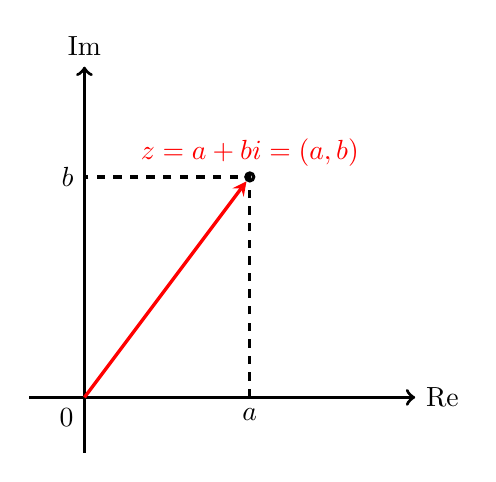
\begin{tikzpicture}[very thick,scale = .7]
      \draw[->] (-1,0) -- (6, 0) node [right] {Re};
      \draw[->] (0,-1) -- (0,6) node [above] {Im};
      \draw (0,0) node [below left] {0};
      \draw (3,0) node [below] {$a$} [dashed] -- (3,4) -- (0,4) node [left] {$b$};
      \draw[-stealth, %% changer la flèche droite
      shorten >=2pt, %% raccourcir légèrement
      color=red] (0,0) -- (3,4) %
      % node [midway,above left,color=black] {$\module{z}$} %
      node [above] {$z = a+bi = (a,b)$}; %
      \draw (3,4) circle (2pt); % Marquer le point.
      % \begin{scope}
      %   \path[clip] (0,0) -- (3,0) -- (3,4) -- cycle;
      %   \draw (0,0) circle (1) (1,.7) node [right] {$\arg z$};
      % \end{scope}
    \end{tikzpicture}
  \end{center}\pause
  La plupart des opérations sur les nombres complexes auront leur interprétation géométrique dans ce plan.
\end{frame}
%\url{http://fr.wikipedia.org/wiki/Fichier:Complex_number.svg}
%\url{http://fr.wikipedia.org/wiki/Fichier:Complex_number_illustration.svg}


% \begin{prop}
%   Pour tout $z = a+bi$ et $z^\prime = a^\prime + b^\prime i$ nombres complexes, on a
%   \begin{enumerate}
%   \item $z \bar z = a^2 + b^2$;
%   \item $\bbar{z} = z$;
%   \item $\module z = \module {\bar z}$;
%   \item $\overline{z z'} = \bar z \bar{z'}$ et $\module{zz^\prime} = \module z \module{z^\prime}$;
%   \item $\module{z+z^\prime} \leq \module z + \module{z^\prime}$.
%   \end{enumerate}
% \end{prop}

\section{Op\'erations}
\subsection{Somme}
\begin{frame}
  Puisque des nombres complexes sont des couples de réels, nous avons~:\pause
  \begin{property}
    La \Defn{somme} de deux nombres complexes\pause{} \(z = a+bi\) et \(z' = c+di\) est\pause
    \begin{equation*}
      z+z' \pardef (a+c)+(b+d)i
    \end{equation*}
  \end{property}

  L'addition des nombres complexes a les propriétés suivantes~: \pause
  \begin{property}Pour tout $z,z',z"\in \CC$~:\pause
    \begin{itemize}[<+->]
    \item \((z + z') + z'' = z + (z' + z'')\) (associativité) ;
    \item \(z + z' = z' + z\) (commutativité) ;
    \item \(z + 0 = z\) (existence d'un neutre : 0) ;
    \item \(z + (-z) = 0\) (existence d'un opposé) ;
    \end{itemize}
    où\pause{} $0$ est le complexe $0+0i$,\pause{} et \(-z\) est le complexe obtenu à partir de \(z = a+ib\) comme suit~:\pause{} \(-z = -a - ib\).
  \end{property}
\end{frame}

\begin{frame}
  \begin{example}
    \begin{itemize}[<+->]
    \item \((1+i) + (2 + i) = 3 + 2i\)
    \item \((-1+i) + (3 - i) = 2\)
    \item \(-1+2i + 1 + 2i = 4i\)
    \end{itemize}
  \end{example}\pause

\begin{block}{Interprétation géométrique}
  Soit \(z_{0} \in \CC\).\pause{} L'application \(z \mapsto z_{0} + z\) correspond à\pause{} une translation.
\end{block}
\end{frame}

\subsection{Produit}
\begin{frame}
  \begin{definition}
    Comme annoncé, le produit sur \(\CC\) est défini par~:\pause
    \begin{equation*}
      (a+ib)(x+iy) = ax - by + i (ay+bx).
    \end{equation*}
  \end{definition}

  \begin{remark*}
    Dans le cas particulier où $b = 0$,\pause{} la multiplication de $(x+yi)$ par un réel $a$\pause{} donne précisément le \og produit par un scalaire\fg{} usuel sur $\RR^2$.
  \end{remark*}
  \begin{example}\pause
    \begin{equation*}
      i^{2} = (0+i)(0+i) = (0 - 1) + 0i = -1
    \end{equation*}
  \end{example}
\end{frame}

\begin{frame}
  Le produit des nombres complexes a les propriétés suivantes~:\pause
  \begin{property}Pour tous $z,z',z''\in \CC$~:\pause
    \begin{itemize}[<+->]
    \item \((z z') z'' = z (z' z'')\) (associativité) ;
    \item \(z z' = z' z\) (commutativité) ;
    \item \(1z = z\) (existence d'un neutre : 1) ;
    \item Si $z\neq 0$, il existe $z^{-1}$ tel que \(z z^{-1} = 1\) (existence d'un inverse) ;
    \item \(z(z'+z") = z z' + z z"\) (distributivité par rapport à l'addition).
    \end{itemize}
  \end{property}
\end{frame}

\begin{frame}
  \begin{proof}
    Faisons, pour l'exemple, la commutativité~:\pause{} notons \(z = a+ib\) et \(z' = x+iy\) et calculons\pause
    \begin{equation*}
      (a+ib)(x+iy) = ax - by + i (ay+bx)
    \end{equation*}\pause
    tandis que
    \begin{equation*}\pause
      (x+iy)(a+ib) = xa - yb + i (ya+xb).
    \end{equation*}\pause
    Les membres de droite sont égaux dès lors nous avons le résultat.\pause
    
    Seule l'existence de l'inverse $z^{-1}$ est laissée en suspend !
  \end{proof}
\end{frame}

\begin{frame}
\begin{remark*}
  On peut \og oublier\fg{} la formule du produit complexe\pause{} et se contenter de distribuer et d'utiliser la règle \(i^{2} = -1\)~:\pause
  \begin{align*}
    \uncover<+->{(a+ib)(x+iy) &= ax + aiy + ibx + ibiy\\}
    \uncover<+->{&= ax + i(ay + bx) + by i^{2}\\}
    \uncover<+->{&= ax - by + i(ay+bx).}
  \end{align*}
\end{remark*}\pause
\begin{example}
    \begin{itemize}[<+->]
    \item \(12 (2 + i) = 24 + 12i\)
    \item \((2-i)(4+i) = 9 - 2i\)
    \item \((1+i)(1+i) = 2i\)
    \item \((1+i)(1-i) = 2\)
    \end{itemize}
  \end{example}
\end{frame}
\begin{frame}
  L'application produit $(x,y) \mapsto (a,b)(x,y)$ s'interpète comme suit:\pause
  \begin{block}{Interprétation géométrique}
    Notons :
    \begin{equation*}
      (a,b) = \rho (\cos \theta,\sin \theta)
    \end{equation*}\pause
    où $\rho \geq 0$ et $\theta \in \interco{0,2\pi}$ sont les coordonnées polaires du point $(a,b)$.\pause

    Alors $(x,y)\mapsto(a,b)(x,y)$ est la composée de~:\pause
    \begin{itemize}[<+->]
    \item une rotation d'angle $\theta$, et
    \item une homothétie de rapport $\rho$.
    \end{itemize}
  \end{block}
\end{frame}

\subsection{Conjugaison}
\label{sec:conjugaison}
\begin{frame}{Conjugaison}\pause
\begin{definition}
  Si \(z = a+ib\) est un nombre complexe\pause{}, on définit son \Defn{conjugué} par\pause
  \begin{equation*}
    \conj{z} = a-ib.
  \end{equation*}
\end{definition}

\begin{example}Quelques examples~:\pause
  \begin{itemize}[<+->]
  \item \(\conj {2 + i} = 2 - i\)
  \item \(\conj {2 - i} = 2 + i\)
  \item \(\conj {3 + 2i(1-5i)} = \conj{3 + 2i - 10 i^{2}} = \conj{13 + 2i} = 13 - 2i\)
  \end{itemize}
\end{example}
\end{frame}

\begin{frame}
  \begin{property}La conjugaison complexe vérifie~:\pause
    \begin{itemize}[<+->]
    \item \(\conj{z+z'} = \conj[z'] z + \conj{z'}\)
    \item \(z = \conj {\conj z}\) (involutivité)
    \item \(\conj{zz'} = \conj z \conj{z'}\)
    \item \(\conj{z^{2}} = \conj z^{2}\) ; \(\conj {z^{3}}= \conj z ^{3}\) ; etc.
    \end{itemize}
  \end{property}\pause
  \begin{proof}
    Notons \(z = a+ib\) et \(z' = x+iy\) et prouvons la première propriété~:
    \begin{align*}
      \uncover<+->{\conj{z + z'} &= \conj{(a+ib)+(x+iy)}}
                                   \uncover<+->{= \conj{a+x + i(b+y)}}
                                   \uncover<+->{= a+x - i (b+y)\\}
      \uncover<+->{&= a - i b + x - iy}
                     \uncover<+->{= \conj z + \conj z'.}
    \end{align*}
  \end{proof}
\end{frame}

\subsection{Module}
\label{sec:module}
\begin{frame}
\begin{remark*}\pause
  La conjugaison complexe a une propriété que nous n'avons pas encore mentionnée~:\pause{} si \(z =a+ib\), alors\pause
  \begin{equation*}
    z \conj z = (a+ib)(a-ib) = a^{2} + b^{2}.
  \end{equation*}\pause
  Le produit d'un nombre complexe avec son conjugué est donc\pause{} un nombre réel\pause{}, et ce réel est nul si et seulement si \pause{}\(z\) est le nombre complexe nul \pause{}(c'est-à-dire \(a = b = 0\)).
\end{remark*}

\begin{definition}
  Le \Defn{module} de \(z = a+bi\) est\pause{} le nombre réel\pause{} noté \(\abs z \pardef \sqrt{z\conj z} = \sqrt{a^{2} + b^{2}}\).\pause
\end{definition}
\end{frame}
\begin{frame}
  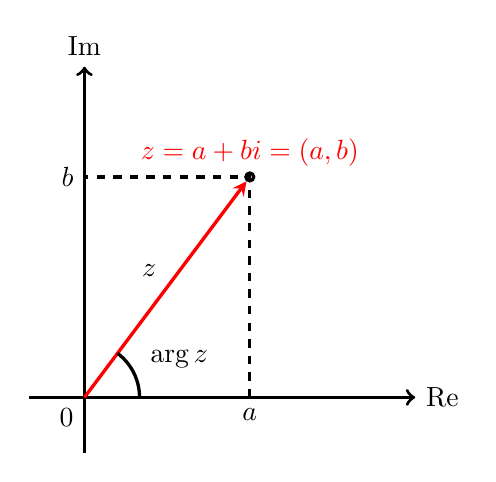
\begin{tikzpicture}[very thick,scale = .7]
    \draw[->] (-1,0) -- (6, 0) node [right] {Re};
    \draw[->] (0,-1) -- (0,6) node [above] {Im};
    \draw (0,0) node [below left] {0};
    \draw (3,0) node [below] {$a$} [dashed] -- (3,4) -- (0,4) node [left] {$b$};
    \draw[-stealth, %% changer la flèche droite
    shorten >=2pt, %% raccourcir légèrement
    color=red] (0,0) -- (3,4) %
    node [midway,above left,color=black] {$\module{z}$} %
    node [above] {$z = a+bi = (a,b)$}; %
    \draw (3,4) circle (2pt); % Marquer le point.
    \begin{scope}
      \path[clip] (0,0) -- (3,0) -- (3,4) -- cycle;
      \draw (0,0) circle (1) (1,.7) node [right] {$\arg z$};
    \end{scope}
  \end{tikzpicture}
\end{frame}

\begin{frame}
  \begin{property}Les propriétés suivantes sont vérifiées pour tous \(z,z'\in\CC\)~:\pause
    \begin{itemize}[<+->]
    \item \(\abs{zz'} = \abs z \abs{z'}\)
    \item \(\abs{z+z'} \leq \abs z + \abs{z'}\)
    \item \(\abs z \geq 0\)
    \item \(\abs z = 0 \iff z = 0\)
    \end{itemize}
  \end{property}
  \begin{proof}\pause
    Pour la première propriété, notons \(z = a+ib\) et \(z' = c+id\)\pause
    \begin{equation*}
      zz' = ac -bd + i(ad+bc)
    \end{equation*}\pause
    dès lors le module au carré vaut\pause
    \begin{equation*}
      (ac-bd)^{2} + (ad+bc)^{2}\pause = a^{2}c^{2} - 2 abcd + b^{2} d^{2} + a^{2}d^{2}+b^{2}c^{2} + 2 abcd
    \end{equation*}\pause
    et par ailleurs
    \begin{equation*}
      \abs z^{2} \abs{z'}^{2} = (a^{2} + b^{2})(c^{2} + d^{2}) \pause = a^{2}c^{2} + a^{2} d^{2} + b^{2} c^{2} + b^{2} d^{2}
    \end{equation*}\pause
    La seconde propriété\pause{} est l'inégalité triangulaire.
  \end{proof}
\end{frame}

\begin{frame}
\begin{remark*}
  En particulier, si $z = a + 0i$ est réel\pause{}, le module de \(z\) est\pause{} $\sqrt{a^{2} + 0^{2}} \pause= \abs a$. C'est la valeur absolue !

  Ceci justifie d'utiliser une même notation $\abs\cdot$ pour les deux notions.
\end{remark*}
\end{frame}


% \begin{remark*}
%   Puisque \(z \conj z = a^{2} + b^{2}\)
% \end{remark*}

\subsection{Inverse}
\begin{frame}
\begin{rappel}
  Nous avons annoncé que chaque nombre complexe non-nul admettait un inverse.\pause
\end{rappel}

Comme
\begin{equation*}
  z \conj z = a^{2} + b^{2}
\end{equation*}\pause
nous en déduisons
\begin{equation*}
  z \frac{\conj z}{a^{2}+b^{2}} = 1
\end{equation*}\pause
ce qui montre que
\begin{equation*}
  z^{-1}= \frac 1z = \frac{\conj z}{a^{2}+b^{2}}
\end{equation*}
est bien l'inverse du nombre complexe $z$.\pause

Nous pourrions écrire également~:\pause
\begin{equation*}
  z^{-1}= \frac 1z = \frac{\conj z}{z \conj z}
\end{equation*}\pause
ce qui est très simple à mémoriser.
\end{frame}
\subsection{Exponentiation}
\begin{frame}
  Nous avons les propriétés suivantes~:\pause
  \begin{align*}
    \uncover<+->{(a+ib)^{2}  & = a^{2} - b^{2} + 2iab \\}
    \uncover<+->{(a + b i)^3 & = a^3 - 3 a b^2 + i (3 b a^2 - b^3) \\}
    \uncover<+->{&\vdots}
  \end{align*}\pause
  Ces formules découlent simplement de la distributivité.
\end{frame}
\subsection{Racines carrées, cubiques, \dots}
\begin{frame}
  \begin{rappel}
    Si \(r \in \RR^{+}\),\pause{} \(\sqrt r\) est l'unique\pause{} nombre réel\pause{} positif\pause{} dont le carré vaut \(r\).
  \end{rappel}
  
  \begin{remark*}
    Dans \(\CC\), il n'existe pas de notion de \og positif\fg{} ou \og négatif\fg{},\pause{} et la notation \(\sqrt{z}\) \pause{}\emph{n'est en général pas définie} pour \(z \in \CC\).
  \end{remark*}
  
  Cependant, pour un \(z \in \CC\) donné\pause{}, nous pouvons parler \emph{des} racines carrées (ou cubiques, etc.) de \(z\).\pause

  \begin{definition}
    Un complexe \(a+ib\) est \emph{une} racine carrée de \(z = x+iy\) si \((a+ib)^{2} = x+iy\).\pause{} En d'autres termes, il faut et suffit que\pause{} \(a^{2}-b^{2} = x\) et \(2ab = y\).
  \end{definition}
  
  \begin{remark*}
    De même pour les racines cubiques, et de manière générale pour les racines \(n\)\ieme.
  \end{remark*}
\end{frame}
\begin{frame}
  \begin{example}
    Calculons les racines carrées de $3+4i$.\pause{} Notons $a+bi$ une telle racine carrée, avec $a$ et $b$ réels.\pause

    On résout~:
    \begin{equation*}
      \begin{systeme}
        a^{2}-b^{2} & 3\\
        2ab & 4
      \end{systeme}
    \end{equation*}
    ce qui donne\pause{} $ab = 2$, et\pause{} (en multipliant la première équation par $a^{2}$)\pause{} $a^{4} - 4 - 3 a^{2} = 0$\pause{}, soit $a^{4} - 3 a^{2} - 4 = 0$.\pause

    Dès lors $a^{2} = \frac{3 \pm \sqrt{9 + 16}}{2}$\pause{} soit $a^{2} = 4$\pause{} (l'autre solution est négative)\pause{}.

    On en déduit $a = 2$ ou $a = -2$.\pause{} Comme $ab = 2$, les solutions sont~:\pause
    \begin{equation*}
      -2 - i\qquad \text{et} \qquad 2 + i
    \end{equation*}
  \end{example}\pause
  \begin{remark*}\pause
    Nous verrons une autre méthode pour calculer des racines (carrées, cubiques, etc.).
  \end{remark*}
\end{frame}
\course{29}% Complexes
\subsection{Argument}
\label{sec:argument}
\begin{frame}
\begin{rappel}
  Si $z$ est un nombre complexe, il s'écrit $a+ib$ pour certains réels $a$ et $b$.\pause

  Si $\rho$ et $\theta$ sont les coordonnées polaires du point $(a,b)$ du plan\pause{}, on a vu $\rho = \module z$.
\end{rappel}\pause

\begin{definition}
  L'\Defn{argument} d'un nombre complexe \(z\),\pause{} noté $\arg z$,\pause{} est l'angle polaire de \(z\) vu comme un point du plan de Gauß.
\end{definition}\pause

\begin{remark*}
Nous savons que la mesure de cet angle n'est défini qu'à un multiple entier de \(2\pi\) près !\pause{}  Généralement on prend $\arg z$ entre $0$ et $2\pi$\pause{} (on parle alors de détermination principale)\pause{} ou alors entre $-\pi$ et $\pi$.\pause
\end{remark*}

\begin{alertblock}{}\pause
L'argument du nombre complexe nul n'est pas défini.
\end{alertblock}
\end{frame}
\begin{frame}
  \begin{center}
  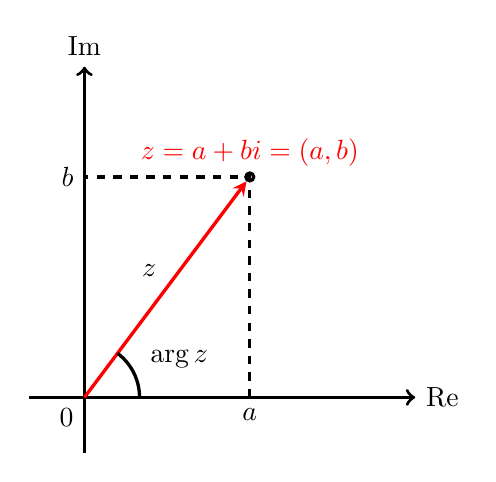
\begin{tikzpicture}[very thick,scale = .7]
    \draw[->] (-1,0) -- (6, 0) node [right] {Re};
    \draw[->] (0,-1) -- (0,6) node [above] {Im};
    \draw (0,0) node [below left] {0};
    \draw (3,0) node [below] {$a$} [dashed] -- (3,4) -- (0,4) node [left] {$b$};
    \draw[-stealth, %% changer la flèche droite
    shorten >=2pt, %% raccourcir légèrement
    color=red] (0,0) -- (3,4) %
    node [midway,above left,color=black] {$\module{z}$} %
    node [above] {$z = a+bi = (a,b)$}; %
    \draw (3,4) circle (2pt); % Marquer le point.
    \begin{scope}
      \path[clip] (0,0) -- (3,0) -- (3,4) -- cycle;
      \draw (0,0) circle (1) (1,.7) node [right] {$\arg z$};
    \end{scope}
  \end{tikzpicture}
\end{center}

\end{frame}
\begin{frame}
  \begin{example}Voici la détermination principale des arguments de quelques complexes~:\pause
    \begin{itemize}[<+->]
    \item \(\arg i = \uncover<+->{\frac \pi 2}\) ;
    \item \(\arg r = \uncover<+->{0}\) si \(r\) est un réel positif ;
    \item \(\arg r = \uncover<+->{\pi}\) si \(r\) est un réel strictement négatif.
    \item \(\arg(1+i) = \uncover<+->{\frac\pi4}\) ;
    \end{itemize}
  \end{example}

  \begin{example}
    Le nombre complexe \(z = \rho(\cos \theta + i \sin \theta)\)\pause{} a pour argument \(\theta\) (et pour module $\rho$).\pause
  \end{example}\pause

  \begin{property}Pour des complexes \(z\) et \(z'\) \pause{} (à un multiple entier de \(2\pi\) près)~:\pause
    \begin{align*}
      \arg (zz') &= \arg z + \arg z'
    \end{align*}\pause
    (cas particulier~: $\arg (-z) = \pi + \arg z$)
  \end{property}
\end{frame}

\begin{frame}
  De façon générale, l'argument d'un complexe $z = a+ib$ se détermine via les formules\pause
  \[\frac a {\module z} = \cos(\arg(z)) \quad \frac b {\module z} = \sin(\arg(z))\]
  \pause{}ou encore par la formule\pause
  \[\frac b a = \tan(\arg(z)) \quad \text{en vérifiant le quadrant.}\]%

  \begin{example}\pause
    L'argument $\theta$ de $z = -1 - i$ vérifie
    \begin{equation*}
      \tan \theta = \frac{-1}{-1} = 1
    \end{equation*}\pause
    Or $z$ est dans le troisième quadrant (\pause{}en bas à gauche)\pause{}, donc
    \begin{equation*}
      \theta = \frac{\pi}{4} + \pi\pause = \frac{5\pi}{4}
    \end{equation*}
  \end{example}
\end{frame}

\section{Forme polaire ou trigonométrique}
\begin{frame}
  \begin{remark*}
    Dans le plan de Gauß, un complexe $z$ représente un point.\pause
    Le passage des coordonnées polaires $(\rho, \theta)$ aux coordonnées
    cartésiennes $(a,b)$ donne deux formules équivalentes\pause
    \begin{equation*}
      a + bi \quad\uncover<+(1)->{=}\quad \rho \left(\cos (\theta) + i \sin (\theta)\right)
    \end{equation*}\pause
  \end{remark*}

  \begin{definition}
    La première formule \(a+ib\) est généralement appelée\pause{} \Defn{forme normale} ou \Defn{forme cartésienne},\pause{} et la seconde\pause{} est la \Defn{forme polaire} ou \Defn{forme trigonométrique},\pause{} ou encore (voir ci-dessous) \Defn{forme exponentielle}.
  \end{definition}
\end{frame}

\begin{frame}
  La notation $z = \rho \paren*{\cos (\theta) + i \sin (\theta)}$ est un peu longue,\pause{} mais il existe des raccourcis.\pause
  Le plus courant est la forme exponentielle :\pause
  \begin{definition}
    On définit
    \begin{equation*}
      \exp{\paren{i\theta}} \pardef \cos(\theta) + i \sin(\theta).
    \end{equation*}\pause
    et on peut alors noter $z$ sous \Defn{forme exponentielle} :\pause
    \begin{equation*}
      z= \rho \exp{\paren{i\theta}}
    \end{equation*}
  \end{definition}\pause
  \begin{remark*}
    Une autre notation, mais que nous n'utiliserons pas dans ce cours, est:
    \begin{equation*}\pause
      \cis\paren{\theta} \pardef \cos(\theta) + i \sin(\theta).
    \end{equation*}\vspace{-1ex}
  \end{remark*}\pause
  \begin{remark}
    Avec cette définition\pause{}, la notation $z = \rho \exp{\paren{i\theta}}$ garde un sens si $\rho$ est négatif\pause{}, mais alors $\module z = - \rho$ et \(\arg z = \theta + \pi\)
  \end{remark}
\end{frame}

\begin{frame}
\begin{example}
  Voyons quelques formes polaires~:\pause
  \begin{align*}
    \uncover<+->{1 &=}
                     \uncover<+->{\exp{\paren{i0}}\\}
    \uncover<+->{i &=}
                     \uncover<+->{\exp{\paren*{i\frac\pi2}}\\}
    \uncover<+->{-1 &=}
                      \uncover<+->{\exp{\paren{i\pi}}\\}
    \uncover<+->{1+\sqrt 3 i &=}
                               \uncover<+->{2\exp{\paren*{i \frac\pi3}}}
  \end{align*}
\end{example}
\end{frame}

\begin{frame}
\begin{property}\pause
  Si $z = \rho \exp{\paren{i\theta}}$ et $z^\prime = \rho^\prime \exp{\paren{i\theta^\prime}}$ sont deux nombres complexes\pause{}, si $n$ un entier\pause{}, on a~:
  \begin{enumerate}[<+->]
  \item $\conj z = \rho \exp{\paren{-i \theta}}$;
  \item $\frac1{\rho \exp{\paren{i\theta}}} = \frac1\rho \exp{\paren{-i \theta}}$;
  \item $(\rho \exp{\paren{i\theta}})(\rho^\prime \exp{\paren{i \theta^\prime}}) = \rho \rho^\prime \exp{\paren{i(\theta + \theta^\prime)}}$;
  \item $\left(\rho \exp{\paren{i\theta}}\right)^n = \rho^n \exp{\paren{i n \theta}}$.
  \end{enumerate}
\end{property}
La dernière formule prend parfois le nom de \og De Moivre\fg.\pause

On comprend l'intérêt de la notation exponentielle, puisque les opérations décrites\pause{} deviennent de simples applications des règles sur les exposants.
\end{frame}

\begin{frame}
\begin{proof}
  Vérifions la formule du produit (troisième propriété)~:\pause
  \begin{align*}
    \uncover<+->{(\rho \exp{\paren{i\theta}})(\rho^\prime \exp{\paren{i \theta^\prime}}) & = \rho (\cos(\theta) + i \sin(\theta)) \rho' (\cos(\theta') + i \sin(\theta'))\\}
    \uncover<+->{&= \rho \rho' \paren*{\cos(\theta)\cos(\theta') - \sin(\theta)\sin(\theta')} \\
    \uncover<+->{& \qquad + i (\cos(\theta)\sin(\theta') + \sin(\theta)\cos(\theta'))}\\}
    \uncover<+->{&= \rho \rho' (\cos(\theta+\theta') + i \sin(\theta+\theta'))\\}
    \uncover<+->{&= \rho \rho' \exp{\paren{i(\theta + \theta')}}.}
  \end{align*}
  Dès lors la formule est démontrée.
\noqed
\end{proof}
\end{frame}

\begin{frame}
\begin{proof}[Preuve, suite.]
  Montrons également la formule de De Moivre, par récurrence:\pause
  \begin{equation*}
    \paren*{\rho \exp{\paren{i\theta}}}^n = \rho^n \exp{\paren{i n \theta}}
  \end{equation*}

  La formule est clairement vraie pour \(n = 1\),\pause{} puisque les deux membres sont égaux pour cette valeur de $n$.\pause

  Supposons maintenant la formule vraie\pause{} pour \(n = k\), où \(k\) est un entier fixé.\pause{} C'est l'hypothèse de récurrence.\pause{} Vérifions la formule pour \(n = k+1\)~:\pause
  \begin{align*}
    \uncover<+->{\paren*{\rho \exp{\paren{i \theta}}}^{k+1} &= \paren*{\rho \exp{\paren{i \theta}}} \paren*{\rho \exp{\paren{i \theta}}}^{k}\\}
    \uncover<+->{&= \paren*{\rho \exp{\paren{i \theta}}} \paren*{\rho^{k} \exp{\paren{i k \theta}}}\\}
    \uncover<+->{&= \paren*{\rho \rho^{k} \exp{\paren{i (\theta + k \theta)}}}\\}
    \uncover<+->{&= \rho^{k+1} \exp{\paren{i (k+1) \theta}}}
  \end{align*}
  ce que nous voulions démontrer.\pause

  Ceci prouve la formule de De Moivre pour $n$ entier naturel.\pause{} On pourrait prouver la formule pour les entiers négatifs en utilisant la conjugaison.
\end{proof}
\end{frame}

\subsection{Fonctions trigonométriques}
\begin{frame}
  Par définition des parties réelles (notée $\Re z$) \pause{} et imaginaires (notée $\Im z$), nous avons~:\pause
  \begin{equation*}
    z = \Re z + i \Im z
  \end{equation*}\pause
  et par la définition du conjugué, nous avons~:\pause
  \begin{equation*}
    \conj z = \Re z - i \Im z
  \end{equation*}\pause
  Nous en déduisons, par addition et soustraction~:\pause
  \begin{align*}
    \uncover<+->{z + \conj z &=  2 \Re z}
                               \uncover<+->{& z - \conj z &=2 i \Im z}
  \end{align*}

  Or \(\exp{\paren{ix}} = \cos x + i \sin x\) dans notre notation.\pause

  Les fonctions trigonométriques\pause{} cosinus et sinus peuvent donc être ré-écrites de la manière suivante~:\pause
  \begin{align*}
    \cos(x) &= \frac{\exp{\paren{ix}} + \exp{\paren{-ix}}}{2} & \sin(x) &= \frac{\exp{\paren{ix}}-\exp{\paren{-ix}}}{2i}
  \end{align*}
\end{frame}

\subsection{Exponentielle complexe}
\begin{frame}
  Nous avons introduit la notation \(\exp{\paren{ix}} = \cos x + i \sin x\) pour tout \(x \in \RR\).\pause{} De manière plus générale, si \(z = a+ib\) est un nombre complexe, nous pouvons définir~:\pause
  \begin{equation*}
    \exp{z} = \exp{\paren{a+ib}} \pardef\pause \exp{\paren{a}} \exp{\paren{ib}}
  \end{equation*}\pause
  Cette nouvelle application \(\exp{\cdot} : \CC \to \CC : z \mapsto \exp z\) vérifie l'identité\pause
  \begin{equation*}
    \exp z \exp {z'} = \exp{\paren{z+z'}}
  \end{equation*}
  pour tous complexes \(z, z'\).
  \begin{proof}\pause
    \begin{align*}
      \uncover<+->{\exp{\paren*{a+ib}} \exp{\paren*{a'+ib'}} &= }
      \uncover<+->{\exp a\exp{ib}\exp{a'}\exp{ib'}\\ &= }
      \uncover<+->{\exp a\exp{a'}\exp{ib}\exp{ib'}\\ &= }
      \uncover<+->{\exp{(a+a')}\exp{\paren*{ib+ib'}}\\ &= }
      \uncover<+->{\exp{(a+a')}\exp{\paren*{i(b+b')}}\\ &= }
      \uncover<+->{\exp{\paren*{(a+a')+i(b+b')}}}
    \end{align*}
  \end{proof}
\end{frame}

\section{Racine \texorpdfstring{$n$}{n}\ieme{} d'un complexe}
\begin{frame}
  \begin{rappel}
    On ne parle jamais de \emph{la} racine carrée d'un nombre complexe, mais \emph{des} racines.
  \end{rappel}

  \begin{definition}\pause
    Soit un entier $n \geq 1$ et $z$ un complexe.\pause{} On appelle \Defn{racine $n$\ieme{}} de $z$\pause{} tout nombre complexe $w$ tel que $w^n = z$.
  \end{definition}\pause
  \begin{rappel}\pause
     Écrire $w = a+ib$ et résoudre en $a$ et $b$ est fort long.\pause
  \end{rappel}
  \begin{theorem}\pause
    Si $z$ est donné sous forme polaire $\rho \exp{\paren{i\theta}}$ ($\rho \geq 0$)\pause{}, alors les racines $n$\ieme{} de $z$ sont les nombres $w_0, \ldots, w_{n-1}$ définis par\pause
    \begin{equation*}
      w_k = \sqrt[n]{\rho}\, \exp{\paren*{i \, \frac{\paren{\theta + 2 k \pi}}{n}}} \qquad\text{où $k = 0, \ldots, n-1$}
    \end{equation*}\pause
    En particulier, si \(z \neq 0\), il y a exactement \(n\) racines \(n\)\ieme{} de \(z\).
  \end{theorem}
\end{frame}

\begin{frame}
  \begin{rappel}
    \begin{equation*}
      w_k = \sqrt[n]{\rho}\, \exp{\paren*{i \, \frac{\paren{\theta + 2 k \pi}}{n}}} \qquad\text{où $k = 0, \ldots, n-1$}
    \end{equation*}
  \end{rappel}\pause
  \begin{proof}
    Il y a deux choses à démontrer :\pause
    \begin{itemize}
    \item \(w_{k}\) est bien une racine \(n\)\ieme{} de \(z\), et\pause
    \item il n'y en a pas d'autres.
    \end{itemize}\pause
    Pour le premier point\pause{} :
    \begin{align*}
      \uncover<+->{w_{k}^{n} &= \rho \exp{\paren{i (\theta + 2k\pi)}}\\}
      \uncover<+->{&= \rho \paren*{\cos(\theta+2k\pi) + i \sin(\theta+2k\pi)}\\}
      \uncover<+->{&= \rho \paren*{\cos(\theta) + i \sin(\theta)}\\}
      \uncover<+->{&= \rho \exp{\paren{i\theta}}}
                     \uncover<+->{= z}
    \end{align*}
    \noqed
  \end{proof}
\end{frame}
\begin{frame}
  \begin{proof}[Suite de la preuve]\pause
    Pour le second point\pause{}, considérons \(w = r \exp{\paren{i\varphi}}\) une racine \(n\)\ieme{} de \(z\).\pause{} Alors \(w^{n} = z\), et en particulier \(r^{n} =\pause \module {w^{n}} =\pause \module z =\pause \rho\).\pause{} Ceci montre déjà que \(r = \sqrt[n]{\rho}\).\pause

    Par ailleurs, puisque \(w^{n} = z\) et \(\rho = r^{n}\),\pause{} il faut également \(\exp{\paren{in\varphi}} = \exp{\paren{i\theta}}\).\pause{} C'est-à-dire~:
    \begin{equation*}
      \cos(n\varphi) = \cos (\theta) \qquad     \sin(n\varphi) = \sin (\theta) 
    \end{equation*}\pause
    Or deux angles ne peuvent avoir même sinus et même cosinus que si\pause{} ils sont égaux à \(2\pi\) près : dès lors,\pause
    \begin{equation*}
      n \varphi = \theta + 2k\pi \text{ pour un certain \(k \in \ZZ\)}.
    \end{equation*}\pause
    d'où \(\varphi = \frac{\theta+ 2k\pi}{n}\) comme annoncé.\noqed
  \end{proof}
\end{frame}
\begin{frame}
  \begin{proof}[Suite de la preuve]
    Reste à vérifier qu'il suffit de prendre \(k = 0, \ldots, n-1\), et\pause{} que les $w_{k}$ correspondant sont tous différents.\pause

    Pour cela, remarquons simplement l'égalité~:
    \begin{align*}
      \uncover<+->{w_{k+n} &= \sqrt[n]{\rho}\, \exp{\paren*{i \, \frac{\theta + 2 (k + n) \pi}{n} }}\\}
      \uncover<+->{&= \sqrt[n]{\rho}\, \exp{\paren*{i \, \paren*{\frac{\theta + 2 k\pi}{n} + 2 \pi} }}\\}
      \uncover<+->{&= \sqrt[n]{\rho}\, \exp{\paren*{i \, \frac{\theta + 2 k \pi}{n} }}&= w_{k}}
    \end{align*}\pause
    Donc que pour toute valeur de \(k\), \(w_{k}\) se trouve parmi \(w_{0}, w_{1}, \ldots, w_{n-1}\).\pause

    %% FIXME: m.q. ils sont tous différents ? on pourrait montrer w_l = w_p ssi l-p = 0 mod n.
  \end{proof}

\small Source pour les images animées présentées en fin de cours :

{\tiny \url{www.iflscience.com/brain/math-gifs-will-help-you-understand-these-concepts-better-your-teacher-ever-did}}
\end{frame}
\course{30}% Complexes -- Fin module T.
\begin{frame}
  \begin{block}{Étudiants du secondaires ?}
    Bienvenue !
  \end{block}\pause

  \begin{block}{Dernier cours du module T !}
    \begin{description}
    \item[INFO1] Cours avec M. Henri Anciaux dès lundi. (Plaine !)
    \item[BIOL1, CHIM1, IRBI1, SCIE1] Le cours continue à la Plaine
    \item[GEOL1, GEOG1] Dernier cours.
    \end{description}
  \end{block}
\end{frame}
\subsection{Racines de l'unité}
\begin{frame}
  \label{sec:racines-de-lunite}
  Un cas particulier est \(z = 1\).\pause{} Dans ce cas, ses racines \(n\)\ieme{} sont~:\pause
  \begin{equation*}
    w_k = \exp{\paren*{i \, \frac{2 k \pi}{n}}} \qquad\text{où $k = 0, \ldots, n-1$}\pause
  \end{equation*}
  et nous pouvons les représenter géométriquement~:\pause
  \begin{center}
    \asyinclude{racinesnieme.asy}
  \end{center}
\end{frame}

\section{Équations}
\begin{frame}
\begin{remark*}
  Dès lors que nous avons de \og nouveaux nombres\fg{}\pause

  nous pouvons résoudre des équations qui les impliquent.
\end{remark*}
\end{frame}
\subsection{Premier degré}
\label{sec:premier-degre}
\begin{frame}
  Considérons l'équation d'inconnue \(z\) suivante~:\pause
  \begin{equation*}
    a z + b = 0
  \end{equation*}\pause
  où \(a,b\in \CC\) sont des constantes données.\pause

  Alors sa solution est \(z = -\frac b a\), car les règles d'addition de multiplication par les complexes sont identiques aux règles sur les réels.
\end{frame}
\subsection{Second degré}
\begin{frame}
Considérons l'équation
\begin{equation*}
  a z^{2} + b z + c = 0 \qquad \text{où } a,b,c\in \CC \text{ et }\pause a \neq 0
\end{equation*}\pause
Comme dans le cas réel, nous transformons cette équation en~:\pause
\begin{equation*}
  a \paren*{ \paren*{z + \frac{b}{2a}}^{2} - \frac {b^{2} - 4ac} {4a^{2}}} = 0
\end{equation*}\pause

Notons \(\omega\) une racinée carrée de \(b^{2} - 4ac\)\pause{} (c'est-à-dire \(\omega^{2}= b^{2} - 4ac\)).\pause
\begin{equation*}
  z = \frac{-b \pm \omega}{2a}
\end{equation*}\pause

\begin{remark*}
  Si \(b^{2} - 4ac = 0\), alors ceci ne produit qu'une seule racine,\pause{} dite \og racine double\fg{} ou \og de multiplicité \(2\)\fg{}.\pause

  Si nous admettons qu'une telle racine compte pour deux~:
\end{remark*}\pause
\begin{theorem}
  Tout polynôme de degré \(2\) admet exactement 2 racines complexes (comptées avec multiplicité).
\end{theorem}
\end{frame}
\subsection{Degrés supérieurs}
\label{sec:degres-superieurs}
\begin{frame}
  Si \(P(z) = a_{n}z^{n} + \cdots + a_{1}z + a_{0}\) est un polynôme de degré \(n\) à coefficients complexes,\pause{} alors nous avons~:
  \begin{definition}\pause
    Une racine \(r\) de \(P\) est de \Defn{multiplicité} \(m\) si\pause{} on peut écrire \(P(z) = (z-r)^{m} Q(z)\),\pause{} où \(Q\) est un polynôme\pause{} (forcément de degré \(n-m\))\pause{} dont \(r\) n'est pas une racine.\pause{} (où $m \geq 1$.)
  \end{definition}
  \begin{theorem}[Théorème fondamental de l'algèbre]\pause
    Tout polynôme de degré \(n\) admet exactement \(n\) racines complexes (comptées avec leur multiplicité).
  \end{theorem}
\end{frame}
\section[EDO du second ordre, coefficients constants]
{Complexes et équations différentielles linéaires à coefficients constants}
\begin{frame}
  Considérons l'équation différentielle ordinaire suivante~:\pause
  \begin{equation*}
    a_{n} y^{n\prime} + a_{n-1} y^{(n-1)\prime} + \cdots + a_{1} y' + a_{0} y = f(x)
  \end{equation*}\pause
  où \(a_{0}, \ldots, a_{n}\) sont des constantes (réelles ou complexes)\pause{} et \(f\) est une fonction donnée.\pause

  Nous avons déjà étudié les cas \(n = 1\) et \(n = 2\) précédemment\pause{} dans le cas réel\pause{}, mais nous allons maintenant discuter brièvement le cas général à l'aide des nombres complexes.\pause
\end{frame}
\subsection{Fonctions réelles à valeurs complexes}
\begin{frame}
Une fonction à valeurs complexes est\pause{} une fonction \(\RR \to \CC\).\pause

Comme \(\CC\) est identifiable à \(\RR^{2}\),\pause{} un certain nombre de définitions se transposent aisément du cas\pause
\begin{center}
\og fonction réelle à valeurs vectorielles\fg{}
\end{center}\pause
au cas\pause
\begin{center}
\og fonction réelle à valeurs complexes\fg{}.
\end{center}\pause

En particulier, la notion de dérivée\pause{} : pour dériver une fonction à valeurs complexes,\pause{} il suffit de dériver en considérant que \(i\) est une constante.\pause{} Ceci revient effectivement à dériver \og composante par composante\fg{}.\pause
\end{frame}

\begin{frame}
\begin{example}Dérivons la fonction \(y\) définie par\pause
  \begin{equation*}
    y(x) = \exp{\paren{\lambda x}},
  \end{equation*}\pause
  où \(x \in \RR\) et \(\lambda \in \CC\).\pause{} Écrivons \(\lambda = a +ib\)~:\pause
  \begin{equation*}
    y(x) = \pause \exp{\paren{ax}}(\cos{bx} + i \sin(bx))
  \end{equation*}\pause
  et donc sa dérivée vaut~:\pause
  \begin{equation*}
    y'(x) =\pause a\exp{\paren{ax}}(\cos(bx) + i \sin(bx)) + \exp{\paren{ax}}(-b\sin(bx) + b i \cos(bx))
  \end{equation*}\pause
  ce que nous pouvons ré-écrire\pause
  \begin{equation*}
    y'(x) = a\exp{\paren{ax}}(\cos(bx) + i \sin(bx)) + bi\exp{\paren{ax}}(i\sin(bx) + \cos(bx))
  \end{equation*}\pause
  et donc
  \begin{equation*}
    y'(x) =\pause (a+bi)\exp{\paren{ax}}(\cos{bx} + i \sin(bx)) =\pause \lambda \exp{\paren{\lambda x}} =\pause \lambda y(x).
  \end{equation*}\pause
  Cet exemple montre que la fonction exponentielle\pause{} suit la même propriété de dérivation que l'exponentielle réelle.
\end{example}
\end{frame}

\subsection{Résolution d'une équation homogène avec les nombres complexes}
\begin{frame}
  Considérons une l'équation linéaire homogène.\pause{} Faisons cela~:
  \begin{equation*}
    a_{n} y^{n\prime} + a_{n-1} y^{(n-1)\prime} + \cdots + a_{1} y' + a_{0} y = 0
  \end{equation*}\pause
  \begin{remark*}
    Nous n'avons pas encore de méthode pour résoudre cette équation en général.
  \end{remark*}\pause
  Cherchons une solution de la forme \(y(x) = \exp{\paren{\lambda x}}\).\pause{} Puisque \(y'(x) = \lambda y(x)\), nous avons \(y"(x) = \lambda^{2}y(x)\), et ainsi de suite.\pause{} Dès lors ce \(y\) sera solution si et seulement si~:\pause
  \begin{equation*}
    a_{n}\lambda^{n} + a_{n-1} \lambda^{n-1} + \cdots + a_{1} \lambda + a_{0} = 0
  \end{equation*}\pause
  ce qui est une équation polynomiale de degré \(n\).\pause{} Elle admet donc \(n\) solutions (comptées avec multiplicités).\pause{} Cette équation est appelée \og équation caractéristique\fg{}.\pause
\end{frame}

\begin{frame}
  Mentionnons à présent le résultat général~:\pause
  \begin{theorem}Les solutions de l'équation\pause
    \begin{equation*}
      a_{n} y^{n\prime} + a_{n-1} y^{(n-1)\prime} + \cdots + a_{1} y' + a_{0} y = 0
    \end{equation*}\pause
    sont les combinaisons linéaires de \(n\) fonctions déterminées comme suit~:\pause{} si \(\lambda_{1}, \ldots, \lambda_{k}\) sont les solutions distinctes de l'équation caractéristique\pause{}, de multiplicité respective \(m_{1}, \ldots, m_{k}\),\pause{} alors il faut considérer\pause
    \begin{align*}
      \uncover<+->{\exp{\paren{\lambda_{1} x}},}
      \uncover<+->{x \exp{\paren{\lambda_{1} x}},}
      \uncover<+->{x^{2} \exp{\paren{\lambda_{1} x}},}
      \uncover<+->{& \ldots,}
                     \uncover<+->{x^{m_{1}-1} \exp{\paren{\lambda_{1} x}}\\}
      \uncover<+->{&\vdots\\}
      \uncover<+->{\exp{\paren{\lambda_{k} x}},}
      \uncover<+->{x \exp{\paren{\lambda_{k} x}},}
      \uncover<+->{x^{2} \exp{\paren{\lambda_{k} x}},}
      \uncover<+->{& \ldots,}
                     \uncover<+->{x^{m_{k}-1} \exp{\paren{\lambda_{k} x}}.}
    \end{align*}
  \end{theorem}
\end{frame}
\begin{frame}
  \begin{example}
    Considérons l'équation différentielle $y'''' = y$.\pause{} Quelles sont ses solutions ?\pause

    Polynôme caractéristique : $\lambda^{4} - 1$.\pause{} Les racines (complexes) sont données par\pause{} : $\exp{\paren*{i\frac{2k\pi}{4}}}$,\pause{} c'est-à-dire\pause
    \begin{equation*}
      \exp{\paren*{0}}, \exp{\paren*{i\frac{\pi}{2}}}, \exp{\paren*{i\pi}}, \exp{\paren*{i\frac{3\pi}{2}}}
    \end{equation*}\pause
    ou encore:\pause{} \begin{math}1, i, -1, -i\end{math}.

    Dès lors la solution générale est combinaison linéaire des fonctions suivantes~:\pause
    \begin{equation*}
      \exp{(x)}, \cos(x), \sin(x), \exp{(-x)},
    \end{equation*}\pause
    à savoir~:\pause
    \begin{equation*}
      y(x)  = A \exp{x} + B \cos(x) + C \sin(x) + D \exp{-x}
    \end{equation*}
  \end{example}
\end{frame}
\begin{frame}
  \begin{example}
    Considérons l'équation différentielle $y'''' + y = 0$.\pause{} Quelles sont ses solutions ?\pause

    Polynôme caractéristique : $\lambda^{4} + 1$.\pause{} Les racines (complexes) sont données par\pause
    \begin{align*}
      \exp{\paren*{i\frac{\pi}{4}}}&&       \exp{\paren*{i\frac{3\pi}{4}}}&&       \exp{\paren*{i\frac{5\pi}{4}}}&&       \exp{\paren*{i\frac{7\pi}{4}}}
    \end{align*}\pause
    ou encore:\pause{} \begin{math}\paren*{\pm \frac{1}{\sqrt{2}} \pm \frac{1}{\sqrt{2}} i} \end{math}.

    Dès lors la solution générale est combinaison linéaire des fonctions suivantes~:\pause
    \begin{align*}
      \exp{\paren*{{\frac{x}{\sqrt{2}}}}}\cos\paren*{\frac{x}{\sqrt{2}}}&&
      \exp{\paren*{{\frac{x}{\sqrt{2}}}}}\sin\paren*{\frac{x}{\sqrt{2}}}\\
      \exp{\paren*{{-\frac{x}{\sqrt{2}}}}}\cos\paren*{\frac{x}{\sqrt{2}}}&&
      \exp{\paren*{{-\frac{x}{\sqrt{2}}}}}\sin\paren*{\frac{x}{\sqrt{2}}}
    \end{align*}
  \end{example}
\end{frame}

\course{31}% Analyse vectorielle -- Début module S
\begin{frame}%% Environ 73 présents.
  \begin{description}
  \item[GEOL2,GEOG2,GEOG3] Soyez les bienvenus !\pause
  \item[INFO1] Changez de forum !\pause
  \item[GEOG1,GEOL1] Vous pouvez rester si vous voulez (mais sinon, le cours est fini pour vous).\pause
  \item[BIOL1,CHIM1,IRBI1,SCIE1] Vous êtes au bon endroit.
  \end{description}
\end{frame}
\section{Analyse vectorielle}
\subsection{Champs de vecteurs}
\begin{frame}<handout:0>
  \begin{definition}
    Un \Defn{champ de patates}\pause{} sur un terrain $A \subset \RR^2$\pause{} est une fonction qui à chaque point de $A$,\pause{} associe la patate qui s'y trouve.\pause
  \end{definition}
  \begin{remark*}
    On définit similairement des champs d'autres choses~:\pause
    \begin{enumerate}[<+->]
    \item fleurs
    \item betteraves
    \item blé
    \item maïs
    \item vecteurs
    \item scalaires
    \item \dots
    \end{enumerate}
  \end{remark*}
\end{frame}
\begin{frame}
  \begin{definition}\pause
    Un \Defn{champ de vecteurs} sur \(A\subset\RR^{n}\)\pause{} est une application\pause
    \begin{equation*}
      f : A \to \RR^{n}
    \end{equation*}\pause
    On note \(f_{1},\ldots,f_{n}\) les différentes composantes de \(f\)\pause{}, c'est-à-dire\pause
    \begin{equation*}
      f(x) = (f_{1}(x), \ldots, f_{n}(x))
    \end{equation*}\pause

    Un \Defn{champ scalaire}\pause{} sur \(A\) est une application\pause
    \begin{equation*}
      F : A \to \RR
    \end{equation*}
  \end{definition}\pause
  \begin{remark*}\pause
    L'interprétation d'un champ de vecteurs\pause{} : \(f(x)\) représente un vecteur basé en \(x\).
  \end{remark*}
\end{frame}
\begin{frame}
  \begin{example}
    Si \(f : \RR^{2} \to \RR^{2} : (x,y) \mapsto (x,y)\) on peut représenter la situation comme suit\pause
    \begin{center}
      \includegraphics[scale=0.8]{cdv-exponentiel-truelen}
    \end{center}
  \end{example}
\end{frame}
\begin{frame}
  \begin{example}[suite de l'exemple]
    En modifiant un peu la longueur des flèches pour y voir plus clair, cela donne\pause
    \begin{center}
      \includegraphics[scale=0.8]{cdv-exponentiel}
    \end{center}\pause
  \end{example}
  \begin{remark*}\pause
    Les champs de vecteurs suivants seront infidèles à la réalité pour cette raison.
  \end{remark*}
\end{frame}
\begin{frame}
\begin{example}
  Si \(f : \RR^{2} \to \RR^{2} : (x,y) \mapsto (-y,x)\) on peut représenter la situation comme suit\pause
  \begin{center}
    \includegraphics[scale=0.8]{cdv-tournant}
  \end{center}
\end{example}
\end{frame}

\subsubsection{Potentiels}
\begin{frame}{Fonctions lisses}
\begin{remark*}
  Si \(F : \RR^{n} \to \RR\) est une application différentiable\pause{} (par exemple considérée comme un champ scalaire)\pause{}, alors le gradient \(\nabla F\)\pause{} est un champ de vecteurs\pause{} : au point \((a,b,c)\)\pause{} on associe le vecteur \(\nabla F_{(a,b,c)}\) en ce point.
\end{remark*}
\end{frame}
\begin{frame}
\begin{example}
  Ci-dessous, nous représentons le champ de vecteurs gradient\pause{} et les courbes de niveau\pause{} pour deux fonctions \(F\) données.\pause
  \begin{center}
  \begin{tabular}{cc}
    \uncover<+->{\includegraphics[scale=.9]{cdv-gradient}} 
    & \uncover<+(1)->{\includegraphics[scale=.9]{cdv-gradient2}}\\
    \uncover<+(-1)->{\mbox{\(F : \RR^{2}\to\RR : (x,y)\mapsto x^{2} + y^{2}\)}}
    & \uncover<+->{\mbox{\(F : \RR^{2}\to\RR : (x,y)\mapsto x^{2} + \cos(y)\)}}
  \end{tabular}
\end{center}
\end{example}
\end{frame}

\begin{frame}
  \begin{definition}
    Si \(f : A \subset \RR^{n} \to \RR^{n}\) est un champ de vecteurs\pause{}, on dit que \(f\) \Defn{dérive d'un potentiel}\pause{} si il existe un champ scalaire\pause{} \(F : A \subset \RR^{n} \to \RR\)\pause{} tel que \(f = \nabla F\).
  \end{definition}\pause

  \begin{example}Le champ de gravité créé par un objet massif (par exemple, la terre)\pause{} est représenté, en chaque point,\pause{} par la force que subirait un objet massif ponctuel d'un kilo situé en ce point.\pause

    La loi de gravitation dit que\pause{} la force de gravitation entre deux objets ponctuels\pause{} est proportionnelle\pause{} au carré de l'inverse de la distance les séparant.
  \end{example}
\end{frame}
\begin{frame}
  
\begin{example}[suite]
  En un point $(x,y,z)$ donné de l'espace\pause{} on peut donc écrire le champ de force en ce point :\pause
  \begin{equation*}
    \frac{-GM}{\sqrt{x^{2}+y^{2}+z^{2}}^{3}} (x,y,z)
  \end{equation*}\pause
  (où $M$ est la masse de l'objet massif considéré, et $G$ est la constante universelle de gravitation.)\pause

  En cherchant une primitive de chaque composante du champ de force,\pause{} on se rend compte que le potentiel\pause
  \begin{equation*}
    F(x,y,z) = \frac{G M}{\sqrt{x^{2}+y^{2}+z^{2}}}
  \end{equation*}
  a pour gradient le champ de force ci-dessus.
\end{example}
\end{frame}
% \begin{frame}
%   On peut %% FIXME: utiliser Taylor ordre 1 pour récupérer la force usuelle, F = mg.
% \end{frame}


\subsubsection{Opérateurs différentiels}
\begin{frame}
Rappelons d'abord que la \Defn{matrice jacobienne}\pause{} d'un champ de vecteurs \(f\) de composantes \((f_{1},\ldots,f_{n})\) est donnée par\pause
\begin{equation*}
  \begin{pmatrix}
    \pder {f_{1}}{x_{1}} & \ldots & \pder {f_{1}}{x_{n}} \\
    \vdots              & \ddots &                      \\
    \pder {f_{n}}{x_{1}} &        & \pder {f_{n}}{x_{n}} \\
  \end{pmatrix}.
\end{equation*}
\end{frame}

\begin{frame}{Divergence}
  \begin{definition}\pause
    La \Defn{divergence} d'un champ de vecteurs \(f : A\subset\RR^{n} \to \RR^{n}\) est donnée par\pause{} le champ scalaire\pause{} défini par
    \begin{equation*}
      \diver f = \pder{f_{1}}{x_{1}} + \pder{f_{2}}{x_{2}} + \ldots + \pder{f_{n}}{x_{n}} 
    \end{equation*}\pause
    La divergence est parfois notée \(\nabla \cdot f\).
  \end{definition}\pause
  \begin{example}\pause
    La divergence du champ de vecteurs \og tournant\fg{}\pause{} \(f(x,y) = (-y,x)\) est nulle.\pause
  \end{example}
  \begin{example}
    La divergence du champ de vecteurs \og sortant\fg{} \(f(x,y) = (x,y)\) vaut \(2\) en chaque point.
  \end{example}
\end{frame}
\begin{frame}
\begin{remark*}
    La divergence en un point mesure\pause{} la tendance qu'ont les vecteurs \pause
    \begin{itemize}
    \item \uncover<+->{à s'éloigner (divergence positive)}, ou
    \item \uncover<+->{à aller (divergence négative)}
    \end{itemize}
    de\uncover<.->{/vers} ce point.
  \end{remark*}
\end{frame}
\begin{frame}
\begin{example}
    La divergence de \(f(x,y) = (x^{3},y^{3})\)\pause{} est le champ scalaire dont la valeur au point \((x,y)\) est\pause{} \(3(x^{2} + y^{2})\).
  \end{example}\pause
\begin{remark*}\pause
  En notant \(\nabla = (\pder{}{x_{1}}, \ldots, \pder{}{x_{n}})\), ce $\nabla$ ressemble à un vecteur donné en composantes.\pause

  Le \og produit scalaire\fg{} de ce \og vecteur\fg{} avec le vecteur\pause{} \(f = (f_{1},\ldots,f_{n})\)\pause{}, donne la divergence.\pause

  La notation \(\cdot\) étant fréquemment utilisée pour noter le produit scalaire,\pause{} ceci explique la notation \(\nabla\cdot f\) pour la divergence.
\end{remark*}
\begin{remark*}
  Le symbole $\nabla$\pause{} est souvent nommé ``opérateur nabla'' en français\pause{}, ou ``del operator'' en anglais.
\end{remark*}
\end{frame}

\begin{frame}{Rotationnel}
La notion de rotationnel\pause{} telle que nous allons la définir n'a de sens que dans l'espace.\pause

\begin{definition}
  Le \Defn{rotationnel} d'un champ de vecteurs \(f : A\subset\RR^{3} \to \RR^{3}\)\pause{} est le champ de vecteurs\pause{} défini par\pause
  \begin{equation*}
    \rot f = \paren*{\pder{f_3}{x_2}-\pder{f_2}{x_3},\pder{f_1}{x_3}-\pder{f_3}{x_1},\pder{f_2}{x_1}-\pder{f_1}{x_2}}
  \end{equation*}\pause
  Le rotationnel est parfois encore noté \(\nabla \times f\).
\end{definition}
\begin{remark*}\pause
  Le rotationnel mesure la tendance qu'on les vecteurs de $f$ à ``tourner'' autour du point $(x_{1},x_{2},x_{3})$.
\end{remark*}
\end{frame}
\begin{frame}
  \begin{remark*}
    Si $f : \RR^2 \to \RR^{2}$,\pause{} on peut définir $\bar f : \RR^3 \to \RR^{3}$\pause{} par
    \begin{equation*}
      \bar{f}(x_{1},x_{2},x_{3}) \pardef\pause \paren*{f_{1}(x_{1},x_2),f_{2}(x_{1},x_2),0}.
    \end{equation*}\pause

    Alors~:
    \begin{equation*}
      \rot \bar{f} = \paren*{0,0,\pder{f_2}{x_1}-\pder{f_1}{x_2}}.
    \end{equation*}
  \end{remark*}\pause

  \begin{definition}
    Le \Defn{rotationnel} d'un champ de vecteurs \(f : A\subset\RR^{2} \to \RR^{2}\) du plan\pause{} est donné par le champ scalaire défini par
    \begin{equation*}\pause
      \rot f = \pder{f_2}{x_1}-\pder{f_1}{x_2}.
    \end{equation*}
  \end{definition}
\end{frame}
\begin{frame}
  \begin{example}
    Le rotationnel du champs de vecteurs $f : \RR^3 \to \RR^3 : (x,y,z) \mapsto (x,y,z)$ est\pause{} $\rot f = 0$.
  \end{example}
  \begin{example}\pause
    Le rotationnel de
    \begin{equation*}
      f(x,y,z) = (-y,x,0)
    \end{equation*}
    est\pause
    \begin{equation*}
      \rot f(x,y,z) = (0,0,2)
    \end{equation*}
  \end{example}\pause
  \begin{remark*}
    En anglais, rotationnel se dit ``curl''.
  \end{remark*}
\end{frame}

\begin{frame}{Laplacien}
  \label{sec:laplacien}
  Le \Defn{laplacien} d'un champ scalaire \(F : \RR^{n} \to \RR\)\pause{} est donné par le champ scalaire défini par\pause
  \begin{equation*}
    \Delta F \pardef \diver (\nabla F)\pause = \pder{^{2}F}{x_{1}^{2}} + \cdots + \pder{^{2}F}{x_{n}^{2}}
  \end{equation*}
\end{frame}

\subsubsection{Composée des opérateurs différentiels}
\label{sec:comp-des-oper}
\begin{frame}
\begin{proposition}
  Si \(F\) est un champ scalaire et \(f\) est un champ de vecteurs\pause{}, tous deux de classe \(\Cclass^{2}\).\pause{} Alors on a les propriétés suivantes~:\pause
  \begin{equation*}
    \rot{\nabla F} = 0 \qquad\pause  \diver {\rot {f}} = 0 \qquad\pause \diver{\nabla F} = \Delta F.
  \end{equation*}\pause
  Si \(F,G\) sont des champs scalaires différentiables, alors~:
  \begin{equation*}\pause
    \nabla{ (F G) } = (\nabla F) G + F (\nabla G).
  \end{equation*}
\end{proposition}
\end{frame}
%% J'ai fait au cours :
%% - dire pourquoi la première relation est évidente : penser à la trajectoire d'une particule dans le champ de force qui dérive d'un potentiel : elle doit toujours gagner (ou perdre, si on met le signe) en "énergie".
%% - le calcul pour la 2e relation
%% - laisser le produit en exercices.
\course{32}% Analyse vectorielle
\begin{frame}
  \begin{block}{Avis aux GEOG2,GEOG3,GEOL2}
    Vous êtes invités à vous greffer à un des deux groupes des BA1 en Biologie

    De préférence le groupe ``1 et 2'' (première séance ``module S'' dans ce groupe : 5 mars)\pause

    Si vous n'avez pas encore accès UV à Math F 112, envoyez moi un mail à \texttt{nrichard@ulb.ac.be}\pause
  \end{block}

  \begin{block}{Avis à tous}
    Un fichier d'exercices pour ce chapitre a été mis en ligne.
  \end{block}
\end{frame}

\section{Intégrales curvilignes}
\requires{chap:fctvalvecto}%Chap7
% \begin{frame}
%   \begin{rappel}
%     L'intégration vise à ``sommer des quantité infinitésimales''.
%   \end{rappel}
% \end{frame}
\begin{frame}
  \begin{rappel}
    Une courbe paramétrée dans \(\RR^{n}\)\pause{} est une application\pause{} continue\pause{} définie sur un intervalle\pause{}, et à valeurs dans \(\RR^{n}\).\pause
\end{rappel}

  Dans cette section nous nous intéressons uniquement aux courbes paramétrées définies sur un intervalle\pause{} fermé\pause{} et borné\pause{}, c'est-à-dire aux paramétrisations de la forme \(\gamma : \intercc{a,b} \to \RR^{n}\).\pause

 Nous supposerons par ailleurs que \(\gamma\) est dérivable\pause{} et que cette dérivée est continue sur \(\interoo{a,b}\),\pause{} sauf éventuellement en un nombre fini de points. \pause

 Dans cette situation, nous dirons que \(\gamma\) est\pause{} \Defn{$\Cclass^{1}$ par morceaux}.
\end{frame}

\begin{frame}
\begin{example}Voici un exemple de courbe a priori \(\Cclass^{1}\) par morceaux.\pause
  \begin{center}
    \includegraphics{C1parmorceaux}
  \end{center}\pause
  On discerne des points où la courbe n'admet pas de tangente,\pause
 ce qui pourrait indiquer qu'elle n'y est pas dérivable.\pause{} En réalité\pause{} une telle image pourrait très bien résulter d'une courbe \(\Cclass^{\infty}\).
\end{example}
\end{frame}
\begin{frame}
\begin{example}
  Si on considère l'exemple explicite \(\gamma(t) = (t^{2}, t^{3})\)\pause{} avec \(t \in \intercc{-1,1}\), nous obtenons l'image suivante~:\pause
  \begin{center}
    \includegraphics[scale=.8]{rebrouss}
  \end{center}\pause
  Le point anguleux se trouve en \((0,0)\),\pause{} c'est-à-dire \(t = 0\).\pause{} Or un calcul montre que \(\gamma\) est clairement dérivable en \(t = 0\).\pause
\end{example}
\begin{remark*}
  Dans l'exemple, notons que la dérivée\pause{} en le point de rebroussement est nulle,\pause{} ce qui empêche de déterminer une droite tangente.
\end{remark*}
\end{frame}

\subsection{Reparamétrisation et orientation}
\begin{frame}
  \begin{definition}
    Une \Defn{reparamétrisation} de \(\gamma : \intercc{a,b} \to \RR^{n}\)\pause{} est une courbe paramétrée \(\eta : \intercc{c,d} \to \RR^{n}\) telle qu'il existe une bijection continue \(\alpha : \intercc{c,d} \to \intercc{a,b}\) avec \(\gamma \circ \alpha = \eta\).\pause
  \end{definition}
  L'idée est de parcourir la même courbe\pause{} (le même ensemble de \(\RR^{n}\))\pause{} à vitesse différente.\pause

  \begin{proposition}Si \(\alpha : \intercc{c,d} \mapsto \intercc{a,b}\) est une bijection continue,\pause{} alors elle est strictement monotone.
  \end{proposition}\pause

  \begin{remark*}
    Il existe donc deux types de re-paramétrisations\pause{} :
    \begin{itemize}[<+->]
    \item celles pour lesquelles l'application \(\alpha\) est croissante, et
    \item celles pour lesquelles elle est décroissante.
    \end{itemize}
  \end{remark*}\pause
  \begin{definition}
    \begin{enumerate}
    \item Dans le premier cas\pause{}, on dit que la reparamétrisation \Defn{préserve l'orientation}.\pause
    \item Dans le second cas\pause{} qu'elle \Defn{change l'orientation} puisque le domaine est parcouru dans l'autre sens.
    \end{enumerate}
  \end{definition}
\end{frame}

\begin{frame}
  \begin{proof}[Preuve de la proposition]
    Supposons par l'absurde que \(\alpha\) n'est pas strictement monotone\pause{} ; cela veut dire que \(\alpha\) n'est
    \begin{itemize}
    \item ni strictement croissante,\pause
    \item ni strictement décroissante.
    \end{itemize}
    \pause

    Ne pas être strictement décroissante revient à trouver\pause{} \(x_{0} < y_{0}\) tels que\pause{} \(\alpha(x_{0})\leq \alpha(y_{0})\)\pause{} ; de plus cette inégalité est stricte car \(\alpha\) est une bijection et \(x_{0}\neq y_{0}\).\pause

    Ne pas être strictement croissante revient à trouver \(x_{1}<y_{1}\)\pause{} tels que \(\alpha(x_{1}) > \alpha(y_{1})\),\pause{} avec inégalité stricte pour la même raison que précédemment.\noqed
  \end{proof}
\end{frame}

\begin{frame}
\begin{proof}[Suite de la preuve]
  Considérons \(T = \set{ (x,y) \in \intercc{c,d}^{2} \telque x < y}\).\pause

  C'est un triangle qui contient les points \((x_{0},y_{0})\) et \((x_{1},y_{1})\).\pause{} Donc il contient le segment joignant ces deux points.\pause{} Considérons alors une paramétrisation de ce segment~:\pause
  \begin{equation*}
    f : \intercc{0,1}\mapsto T  \subset \RR^{2} : t \mapsto (1-t) (x_{0},y_{0}) + t (x_{1},y_{1}) = ((1-t)x_{0} + t x_{1}, (1-t)y_{0} + t y_{1})
  \end{equation*}
  et regardons
  \begin{equation*}\pause
    h : \intercc{0,1} \to \RR : t \mapsto \alpha((1-t)x_{0} + t x_{1}) - \alpha((1-t)y_{0} + t y_{1})
  \end{equation*}\pause
  Alors \(h(0) = \alpha(x_{0})-\alpha(y_{0}) < 0\) et \(h(1) > 0\).\pause

  Par le théorème de la valeur intermédiaire\pause{}, il doit exister \(c \in \interoo{0,1}\)\pause{} tel que \(h(c) = 0\).\pause
  Notons \(f(c) = (x_{c}, y_{c})\), de sorte que \(\alpha(x_{c}) = \alpha(y_{c})\) et donc \(x_{c} = y_{c}\) car \(\alpha\) est une bijection.\pause{} Mais alors comme \(f(c)\in T\),\pause{} on doit avoir \(x_{c} < y_{c}\),\pause{} ce qui est une contradiction.\pause
\end{proof}
\end{frame}

\subsection{Courbes simples}
\begin{frame}
  \begin{definition}Une courbe \(\gamma : \intercc{a,b} \to \RR^{n}\) est dite\pause
    \begin{itemize}
    \item \Defn{fermée}\pause{} si \(\gamma(a) = \gamma(b)\) ;\pause
    \item \Defn{simple}\pause{} si \(\gamma\) est une application injective sur \(\interoo{a,b}\).\pause
    \end{itemize}
  \end{definition}
  \begin{remark*}
    Une courbe simple est donc une courbe qui\pause{} ne s'auto-intersecte pas\pause{}, en d'autres termes la trajectoire ne se recoupe pas\pause{} (sauf éventuellement si la courbe est fermée\pause{}, auquel cas le seul point de recoupement est le point de départ qui est identique au point d'arrivée).
  \end{remark*}
\end{frame}


\begin{frame}
  \begin{theorem}[Théorème de Jordan]
    Toute courbe \(\gamma : [a,b] \to \RR^{2}\) femée et simple du plan\pause{} délimite deux régions,\pause{} l'une bornée et l'autre non.
  \end{theorem}

  \begin{example}
    \begin{center}
      \begin{tabularx}{\linewidth}{XXX}
        \centering\raisebox{-0.5\height}{\includegraphics{cercle-disque}}{}
        & \centering\raisebox{-0.5\height}{\includegraphics{huit-deuxdisques}}{} 
        & \centering\raisebox{-0.5\height}{\includegraphics[width=5cm]{parabola-nointerior}}{} \tabularnewline
          Le cercle délimite un disque et son extérieur
        & Cette courbe n'est pas simple : elle délimite deux régions du plan 
        & Cette courbe n'est pas fermée : elle délimite deux régions infinies.
          \end{tabularx}
        \end{center}
      \end{example}
\end{frame}
    
\begin{frame}
  \begin{definition}
    Une courbe simple fermée est dite \Defn{orientée positivement}\pause{} si la région bornée qu'elle délimite\pause{} se trouve \og à gauche\fg{} en parcourant la courbe.\pause{} Sinon elle est dite orientée négativement.%% FIXME: définition un peu douteuse. que veut dire "à gauche" si on a même pas un vecteur tangent dans l'histoire ? Si c'est "à gauche" à un moment, est à gauche tout le temps, et jamais à droite ?
  \end{definition}\pause
  \begin{example}
    Un cercle parcouru dans le sens trigonométrique est orienté positivement.\pause{} Parcouru dans le sens horlogique, il est orienté négativement.
  \end{example}
\end{frame}

\subsection{Intégration d'un champ scalaire}
\begin{frame}
  \begin{definition}
    L'\Defn{intégrale curviligne} d'une fonction\pause{} \(f : A \subset \RR^{n}\to \RR\)\pause{} le long d'une courbe paramétrée \(\gamma : [a,b] \to \RR^n\)\pause{} (avec $\gamma(t) \in A$ pour tout $t \in \intercc{a,b}$)\pause{} est donnée par\pause
    \begin{equation*}
      \int_{C} f \D{s} \pardef\pause \int_{a}^{b} f(\gamma(t)) \norme{\gamma'(t)}\D t
    \end{equation*}
  \end{definition}\pause

  \begin{remark*}\pause
    En particulier, si $f(\gamma(t)) = 1$\pause{} pour tout $t \in \intercc{a,b}$, ceci fournit la \Defn{longueur de la courbe}.
  \end{remark*}
\end{frame}
\begin{frame}{Justification heuristique pour la longueur}\pause
  Subdivisons le domaine \([a,b]\) en \(n\) parties égales\pause{}, et approchons la longueur par
  \begin{equation*}
    \sum_{i=1}^{n} \norme{\gamma(\sfrac in) - \gamma(\sfrac{(i-1)}{n})}\pause
    = \sum_{i=1}^{n} \frac{\norme{\gamma(\sfrac in) - \gamma(\sfrac{(i-1)}{n})}}{\sfrac1n} \;\frac 1n
  \end{equation*}\pause
  On remarque que lorsque \(n\) est grand\pause{}, la fraction \(\frac{\norme{\gamma(\sfrac in) - \gamma(\sfrac{(i-1)}{n})}}{\sfrac1n}\)\pause{} s'approche de \(\norme{\gamma'(\sfrac in)}\)\pause{}, de sorte que la somme ci-dessus correspond à l'intégrale de Riemann comme annoncé.
\end{frame}

\begin{frame}
  \begin{proposition}
    L'intégrale curviligne d'une fonction ne dépend pas de la paramétrisation de la courbe.
  \end{proposition}\pause
  \begin{proof}[Idée de preuve]
    On considère une courbe paramétrée
    \begin{equation*}
      \gamma : \intercc{a,b} \to \RR^{n}
    \end{equation*}
    et une reparamétrisation
    \begin{equation*}
      \eta \pardef \gamma \circ \alpha
    \end{equation*}
    de $\gamma$,\pause{} où \(\alpha : \intercc{c,d} \mapsto \intercc{a,b}\) est une bijection continue.\pause

    Pour simplifier la preuve, nous supposerons de plus que \(\alpha\) est en fait dérivable.\pause{}%% En fait : comme les chemins sont simples et p.p. dérivables, les dérivées ne peuvent pas toutes s'annuler très longtemps, donc on peut supposer que ll'une d'elle est non nulle, donc la réciproque est dérivable -- ceci oblige alpha à être dérivable aussi.

    Supposons \(\alpha(c) = a\) et \(\alpha(d) = b\) dans un premier temps.\pause{} Dans ce cas, \(\alpha\) est strictement croissante.\pause{} Alors par la formule du changement de variable\pause{}, en posant \(t = \alpha(s)\), on obtient :\pause
    \begin{equation*}
      \int_a^b f(\gamma(t)) \norme{\gamma'(t)}\D t =\pause \int_c^d f(\gamma(\alpha(s))) \norme{\gamma'(\alpha(s))} \alpha'(s)\D s.
    \end{equation*}\noqed{}
  \end{proof}
\end{frame}
\begin{frame}
  \begin{proof}[Suite]
    Comme \(\alpha'(s) > 0\),\pause{} on a
    \begin{equation*}
      \norme{\gamma'(\alpha(s))} \alpha'(s) =\pause \norme{\gamma'(\alpha(s))\alpha'(s)} =\pause \norme{\eta'(s)}
    \end{equation*}
    dès lors l'intégrale vaut\pause
    \begin{equation*}
      \int_a^b f(\gamma(t)) \norme{\gamma'(t)}\D t =\pause \int_c^d f(\eta(s)) \norme{\eta'(s)}\D s
    \end{equation*}\pause
    ce que nous voulions démontrer !
  \end{proof}
\end{frame}

\subsection{Intégrale d'un champ de vecteurs}
\begin{frame}
Soit \(\gamma : [a,b] \to\RR^{n}\) une courbe\pause{} (toujours supposée \(\Cclass^{1}\) par morceaux).\pause{} Soit $f : A \subset \RR^{n} \to \RR^{n}$ un champ de vecteurs défini sur $A$ tel que $C\pardef \Im \gamma \subset A$.\pause
\begin{definition}
  L'intégrale du champ de vecteur $f$ le long de $\gamma$ est donnée par\pause
  \begin{equation*}
    \int_\gamma \scalprod{f}{\D s} \pardef\pause \int_{a}^{b} \scalprod{f(\gamma(t))}{\gamma'(t)}\D t.
  \end{equation*}
\end{definition}
\end{frame}

\begin{frame}
  \begin{remark*}
    L'intégrale \(\int_\gamma \scalprod{f}{\D s}\) dépend de l'orientation de \(\gamma\)
    %% preuve non faite au cours
    :\pause{} si on note $\eta(t) = \gamma(a+b-t)$,\pause{} alors
    \begin{align*}
      \int_{\eta} \scalprod{f}{\D s} &= \int_{a}^{b} \scalprod{f(\eta(t))}{\eta'(t)}\D t\\
      \uncover<+->{&= \int_{a}^{b} \scalprod{f(\gamma(a+b-t))}{-\gamma'(a+b-t)}\D t\\}
      \uncover<+->{&= \int_{b}^{a} \scalprod{f(\gamma(u))}{\gamma'(u)}\D u \quad u = a+b-t\\}
      \uncover<+->{&= - \int_{a}^{b} \scalprod{f(\gamma(u))}{\gamma'(u)}\D u \quad u = a+b-t\\}
      \uncover<+->{&= - \int_{\gamma} \scalprod{f}{\D s}}
    \end{align*}
  \end{remark*}
\end{frame}
\begin{frame}
\begin{remark*}
    Cependant\pause{}, les re-paramétrisations préservant l'orientation\pause{} ne modifient pas l'intégrale. Pour cette raison,\pause{} en notant $C = \im \gamma$\pause{} on utilisera souvent la notation $\int_{C} \scalprod{f}{\D s}$ pour désigner l'intégrale.
  \end{remark*}\pause
  \begin{remark*}
    Les notations \(\D{s}\) et \(\gamma'(t)\D{t}\)\pause{} s'appellent \Defn{élément de longueur}. % non dit au cours.
  \end{remark*}
\end{frame}

\course{33}% Analyse vectorielle
\subsection{Intégrale d'un champ de vecteurs}
\begin{frame}{Rappel}
Soit \(\gamma : [a,b] \to\RR^{n}\) une courbe\pause{} (toujours supposée \(\Cclass^{1}\) par morceaux).\pause{} Soit $f : A \subset \RR^{n} \to \RR^{n}$ un champ de vecteurs défini sur $A$ tel que $C\pardef \Im \gamma \subset A$.\pause
\begin{definition}
  L'intégrale du champ de vecteur $f$ le long de $\gamma$ est donnée par\pause
  \begin{equation*}
    \int_\gamma \scalprod{f}{\D s} \pardef\pause \int_{a}^{b} \scalprod{f(\gamma(t))}{\gamma'(t)}\D t.
  \end{equation*}
\end{definition}
\end{frame}

\begin{frame}
  \begin{remark*}
    L'intégrale \(\int_\gamma \scalprod{f}{\D s}\) dépend de l'orientation de \(\gamma\):\pause
    si on note $\eta(t) = \gamma(a+b-t)$,\pause{} alors
    \begin{align*}
      \uncover<+->{\int_{\eta} \scalprod{f}{\D s}}
      \uncover<+->{&= \int_{a}^{b} \scalprod{f(\eta(t))}{\eta'(t)}\D t\\}
      \uncover<+->{&= \int_{a}^{b} \scalprod{f(\gamma(a+b-t))}{-\gamma'(a+b-t)}\D t\\}
      \uncover<+->{&= \int_{b}^{a} \scalprod{f(\gamma(u))}{\gamma'(u)}\D u \quad u = a+b-t ; \D u = -\D t\\}
      \uncover<+->{&= - \int_{a}^{b} \scalprod{f(\gamma(u))}{\gamma'(u)}\D u\\}
      \uncover<+->{&= - \int_{\gamma} \scalprod{f}{\D s}}
    \end{align*}\pause
    Changer l'orientation change donc, en général, le signe de l'intégrale !
  \end{remark*}
\end{frame}
\begin{frame}
\begin{remark*}
    Cependant\pause{}, les re-paramétrisations préservant l'orientation\pause{} ne modifient pas l'intégrale. Pour cette raison,\pause{} en notant $C = \im \gamma$\pause{} on utilisera souvent la notation $\int_{C} \scalprod{f}{\D s}$ pour désigner l'intégrale.
  \end{remark*}\pause
  \begin{remark*}
    Les notations \(\D{s}\) et \(\gamma'(t)\D{t}\)\pause{} s'appellent \Defn{élément de longueur}.
  \end{remark*}
\end{frame}

\subsubsection{Travail d'une force}
\begin{frame}
\begin{remark*}
  Si \(f\) est un champ de vecteurs représentant un champ de forces,\pause{} alors l'intégrale\pause
  \begin{equation*}
    \tau = \int_C \scalprod{f}{\D s}
  \end{equation*}\pause
  est appelée le \Defn{travail}\pause{} de la force \(f\)\pause{} le long de la courbe \(\gamma\).\pause

  C'est \og l'énergie\fg{} gagnée (\(\tau > 0\))\pause{} ou perdue (\(\tau < 0\))\pause{}, en parcourant la courbe \(\gamma\),\pause{} grâce à (ou à cause de) la force \(f\).
\end{remark*}
\end{frame}

\begin{frame}
  Lorsque la force \(f\) dérive d'un potentiel \(F\),\pause{} nous avons \(f = \nabla F\),\pause{} et donc
  \begin{align*}
    \uncover<+->{\tau &= \int_{a}^{b} \scalprod{(\nabla F)(\gamma(t))}{\gamma'(t)}\D t\\}
    \uncover<+->{&= \int_{a}^{b} \paren{F(\gamma(t))}'\D{t}\\}
    \uncover<+->{&= F(\gamma(b)) - F(\gamma(a))}
  \end{align*}\pause
  c'est-à-dire que le travail ne dépend pas vraiment de la courbe\pause{}, seulement du point de départ \(\gamma(a)\)\pause{} et du point d'arrivée \(\gamma(b)\)\pause{} (et de \(F\)).\pause

  \begin{example}
    La force de gravitation induite par la terre dérive d'un potentiel.\pause{} Le travail de cette force entre deux points de hauteurs respective \(h_{1}\) et \(h_{2}\)\pause{} est \(mg(h_{2}-h_{1})\)\pause{} (ceci est une approximation de la loi de Newton).
  \end{example}
\end{frame}
% \begin{frame}{Détail sur l'approximation d'ordre 1}%% FIXME do this ?
%   Le potentiel de la force de gravitation induite par une planète de masse $M$ est\pause
%   \begin{equation*}
%     E(x,y,z) = \frac{G M}{\sqrt{x^{2}+y^{2}+z^{2}}}\pause = \frac{GM}{R+h}
%   \end{equation*}
%   où $R$ est le rayon de la planète et $h$ la hauteur au dessus de la surface de la planète.
%   \pause

%   Si deux points $p = (x,y,z)$ et $p' = (x',y',z')$ sont à faible distance l'un de l'autre, alors la différence d'énergie entre les points est
%   \begin{equation*}
%     E(p') - E(p) = \D E_{p}(p'-p) = \scalprod{\grad E_{p}}{(p'-p)}
%   \end{equation*}
% \end{frame}

\subsubsection{Intégrale d'une forme différentielle}
\begin{frame}
  Si $f : D \subset \RR^{2} \to \RR^{2} : (x,y) \mapsto (P(x,y),Q(x,y))$ est un champ de vecteurs\pause{}, on note parfois
  \begin{equation*}
    \int_{C} P \D x + Q \D y \pardef\pause \int_{C} \scalprod{f}{\D s}
  \end{equation*}\pause

  L'expression $P \D x + Q \D y$\pause{} est aussi appelée une \Defn{forme différentielle}.\pause
\end{frame}


\begin{frame}
  \frametitle{Intégrale circulaire}
  \begin{remark*}
    Lorsque le domaine d'intégration d'une intégrale curviligne est une courbe fermée,\pause{} le symbole $\oint$ est souvent utilisé.
  \end{remark*}
\end{frame}

%FIXME: vérifier si toutes les notations des exercices sont reprises dans le cours.

\section{Intégrales de surface}
\begin{frame}{Rappel et non-rappel}\pause
  Pour intégrer une fonction de deux variables $f : A \subset\RR^{2} \to \RR$,\pause{} il faut d'abord décrire l'ensemble $A$.\pause

  \begin{definition}%%FIXME: deux dessins (cf print du 16 avril)
    Un domaine \(A \subset \RR^{2}\) est dit \Defn{verticalement simple}\pause{} s'il existe \(a,b\in\RR\) et des fonctions \(g_{1}, g_{2} : \intercc{a,b} \to \RR\) telles que\pause
    \begin{equation*}
      A = \set{ (x,y) \in \RR^{2} \pause\telque x \in \intercc{a,b}\pause, g_{1}(x) \leq y \leq g_{2}(x)}.
    \end{equation*}\pause
    Le domaine est \Defn{horizontalement simple} s'il existe \(c,d\in \RR\)\pause{} et des fonctions \(h_{1},h_{2} : \intercc{c,d}\to\RR\) telles que\pause
    \begin{equation*}
      A = \set{ (x,y) \in \RR^{2} \telque y \in \intercc{c,d},\pause h_{1}(y) \leq x \leq h_{2}(y)}.
    \end{equation*}
  \end{definition}
\end{frame}
\begin{frame}
  \begin{theorem}[Théorème de Fubini, version faible]\pause %% repris de précédemment.
    Soit \(A \subset \RR^{2}\) et \(f : A \to \RR\) continue.\pause
    \begin{itemize}
    \item Si \(A\) est verticalement simple, alors\pause
      \begin{equation*}
        \iint_A f = \iint_{A} f(x,y)\D x \D y =\pause \int_{a}^{b} \paren*{\int_{g_{1}(x)}^{g_{2}(x)} f(x,y)\D y} \D x.
      \end{equation*}\pause
    \item Si \(A\) est horizontalement simple, alors\pause
      \begin{equation*}
        \iint_A f = \iint_{A} f(x,y)\D x \D y =\pause \int_{c}^{d} \paren*{\int_{h_{1}(y)}^{h_{2}(y)} f(x,y)\D x} \D y.
      \end{equation*}
    \end{itemize}
  \end{theorem}
\end{frame}
\begin{frame}
  \begin{example}
    Soit
    \begin{equation*}
      f : A = \set{(x,y) \telque x^{2}+y^{2} \leq 1 \text{ et } x \geq 0} \to \RR : (x,y) \mapsto 2xy^{2}
    \end{equation*}\pause
    On décrit d'abord $A$ sous la forme~:\pause
    \begin{equation*}
      A = \set{(x,y) \telque y \in [-1,1],\pause 0 \leq x \leq \sqrt{1-y^{2}}}\pause
    \end{equation*}
    ce qui nous permet d'écrire\pause
    \begin{align*}
      \uncover<+->{\iint_{A}f &= \int_{-1}^{1} \int_{0}^{\sqrt{1-y^{2}}} 2xy^{2} \D x \D y\\}
      \uncover<+->{&= \int_{-1}^{1} (1-y^{2})y^{2} \D y\\}
      \uncover<+->{&= \frac{4}{15}}.
    \end{align*}
  \end{example}
\end{frame}
\begin{frame}\pause
  \begin{remark*}
    Les domaines considérés par les intégrales doubles jusqu'à présent sont dans $R^{2}$.\pause{} Comment intégrer sur une surface (potentiellement) \og courbe\fg{} de $\RR^{3}$ ?\pause

    Réponse : comme pour les courbes, il faut la paramétrer !
  \end{remark*}\pause
  \begin{remark*}
    Note de traduction : il est de coutume de parler de \og paramétrisation\fg{}.\pause{} Un terme français plus correct serait sans doute \og paramétrage\fg{},\pause{} mais il n'est jamais utilisé.\pause{} En conséquence de quoi, il est courant d'utiliser le verbe \og paramétriser\fg{}.
  \end{remark*}
\end{frame}
\begin{frame}
\begin{definition}\pause
    Une \Defn{surface paramétrée} de l'espace\pause{} est une application \(\sigma : A \subset \RR^{2} \to \RR^{3}\)\pause{} continue sur un domaine fermé \(A\)\pause{}, et de classe \(\Cclass^{1}\) sur l'intérieur de \(A\)\pause{}, telle que \((\partial_{1}\sigma)(u,v) \vecprod (\partial_{2}\sigma)(u,v) \neq 0\)\pause{} pour tout \((u,v)\) dans l'intérieur de \(A\). On suppose de plus que $\sigma$ est injective sur l'intérieur de $A$.
  \end{definition}
  \begin{remark*}\pause
    \begin{itemize}
    \item La condition sur les dérivées assure que les vecteurs tangents ne sont pas parallèles\pause{}, c'est-à-dire qu'il y a bien un \emph{plan} tangent.\pause{} Cela évite les cas dégénérés tels que \(\sigma(u,v) = (u,u,u)\).\pause{} Dans ce cas \(\sigma\) paramétrerait en réalité une courbe !\pause

    \item La condition d'injectivité\pause{} assure qu'un point de la surface n'est jamais visité plus qu'une seule fois.
    \end{itemize}
  \end{remark*}
\end{frame}

\begin{frame}
  \begin{example}
    Considérons \(\sigma\) définie par
    \begin{align*}
      \uncover<+->{\sigma &: \intercc{0,2\pi}\times\intercc{0,\pi} \to \RR^{3} \\}
      \uncover<+->{&: (\varphi,\theta) \mapsto (2\cos(\varphi) \sin(\theta), 2 \sin(\varphi) \sin(\theta), 2\cos(\theta)).}
    \end{align*}\pause
    Ceci paramétrise la sphère de rayon \(2\).
  \end{example}

  \begin{remark*}
    Lorsque le domaine d'intégration d'une intégrale de surface est une surface sans bord\pause{} (par exemple la sphère n'a pas de bord,\pause{} mais une demi-sphère possède un bord),\pause{} le symbole $\oiint$ est souvent utilisé.
  \end{remark*}
\end{frame}

\subsection{Reparamétrisation et orientation des surfaces}
\begin{frame}
  Tout comme dans le cas des courbes, une même surface peut être paramétrisée de plusieurs façons.\pause{} À nouveaux, les paramétrisations tombent en deux classes :\pause
  \begin{itemize}
  \item celles qui préservent l'orientation,\pause
  \item celles qui la changent.
  \end{itemize}\pause

  Pour les courbes, l'orientation est le sens de parcourt.\pause{} Dans le cas des surfaces, cette notion de \og sens de parcourt\fg{} n'existe pas,\pause{} c'est pourquoi nous avons une nouvelle définition pour le cas des surfaces :\pause
  \begin{definition}
    L'\Defn{orientation} d'une surface \(S\) est la donnée d'un champ de vecteur normal unitaire,\pause{} c'est-à-dire\pause{} une application continue de \(\nu : S \to \RR^{3}\)\pause{} dont la valeur en chaque point est un vecteur normal à la surface en ce point.
  \end{definition}\pause
  Il y a donc deux orientations possibles.
\end{frame}
\begin{frame}
\begin{remark*}\pause
  Une surface paramétrée possède une orientation canonique :\pause{} en chaque point \(\sigma(u,v)\)\pause{}, le vecteur \(\nu(u,v)\pardef \frac{(\partial_{1}\sigma)(u,v) \vecprod (\partial_{2}\sigma)(u,v)}{\norme{(\partial_{1}\sigma)(u,v) \vecprod (\partial_{2}\sigma)(u,v)}}\)\pause{} est normal à la surface.\pause{} Attention, échanger les rôles de \(u\) et \(v\) renverse l'orientation !
\end{remark*}\pause

\begin{remark*}
  Dans le cas des surfaces bordant un solide\pause{}, par exemple une sphère\pause{}, le champ de vecteur normal \emph{extérieur}\pause{} (celui qui pointe hors du solide)\pause{} est généralement préféré. %% FIXME picture : cdv extérieur (à la sphère ? au tore ?)
\end{remark*}
\end{frame}

\course{34}% Analyse vectorielle
\begin{frame}
  \begin{remark*}
    Avis aux  GEOL2/GEOG2/GEOG3 :
    \begin{itemize}
    \item Vous n'êtes pas supposés rejoindre les groupes de GEOL1 ou GEOG1.
    \item Un mail a été envoyé pour trouver un horaire de séance d'exercices. Nombre total de réponse : 2.
    \end{itemize}
  \end{remark*}
\end{frame}
\begin{frame}{Rappel}
\begin{definition}
  L'\Defn{orientation} d'une surface \(S\) est la donnée d'un champ de vecteur normal unitaire,\pause{} c'est-à-dire\pause{} une application continue de \(\nu : S \to \RR^{3}\)\pause{} dont la valeur en chaque point est un vecteur normal à la surface en ce point.
\end{definition}
\begin{example}
  Dans le cas de la sphère de rayon \(R > 0\)\pause{}, la paramétrisation en coordonnées sphériques donnée ci-dessus~:\pause
  \begin{equation*}
    \sigma(\varphi,\theta) = (R\cos(\varphi) \sin(\theta), R \sin(\varphi) \sin(\theta), R\cos(\theta)).
  \end{equation*}\pause
  donne une orientation canonique à la sphère, que nous calculons.\pause{} Il nous faut d'abord les dérivées partielles~:
  \begin{align*}
    \uncover<+->{(\partial_{1}\sigma)(\varphi,\theta) &= (-R \sin(\varphi) \sin(\theta), R \cos(\varphi) \sin(\theta), 0) \\}
    \uncover<+->{(\partial_{2}\sigma)(\varphi,\theta) &= (R\cos(\varphi) \cos(\theta), R \sin(\varphi) \cos(\theta), - R\sin(\theta))}
  \end{align*}\pause
  ce qui donne le produit vectoriel~:
\end{example}
\end{frame}
\begin{frame}
\begin{example}
\begin{align*}
    \uncover<+->{&(\partial_{1}\sigma)(\varphi,\theta) \vecprod (\partial_{2}\sigma)(\varphi,\theta) \\}
    \uncover<+->{&= (- R^{2} \cos(\varphi) \sin(\theta)^{2}, -R^{2} \sin(\varphi)\sin(\theta)^{2},\\
      & \hspace{2cm}    - R^{2} \sin(\varphi)^{2} \sin(\theta)\cos(\theta) - R^{2} \cos(\varphi)^{2} \sin(\theta)\cos(\theta)) \\ }
    \uncover<+->{&= (- R^{2} \cos(\varphi) \sin(\theta)^{2}, -R^{2} \sin(\varphi)\sin(\theta)^{2}, - R^{2} \sin(\theta)\cos(\theta)).}
  \end{align*}\pause
  La norme vaut \(R^{2}\sin(\theta)\)\pause{} (puisque \(\theta\in\intercc{0,\pi}\), le sinus est positif)\pause{}, et donc le vecteur normal unitaire vaut~:\pause
  \begin{equation*}
    (- \cos(\varphi) \sin(\theta), - \sin(\varphi)\sin(\theta), - \cos(\theta))\pause = \frac{-1}{R}\sigma(\varphi,\theta)
  \end{equation*}\pause
  C'est donc le champ de vecteur normal unitaire \og intérieur\fg{}.
\end{example}
\end{frame}

\begin{frame}{Graphe d'une fonction de deux variables}
  \begin{example}\pause
    Le graphe de \(g : A \subset \RR^{2}\to\RR\) est une surface\pause{} qui peut être paramétrée par\pause
    \begin{equation*}
      \sigma(u,v) = (u,v,g(u,v)).
    \end{equation*}\pause
      L'orientation de cette paramétrisation est donnée par\pause{} $(1,0,\pder g u(u,v))\vecprod (0,1,\pder g v(u,v))$\pause{} dont la troisième composante vaut toujours $1$\pause{} dès lors elle est toujours orientée \og vers le haut\fg{}.
  \end{example}
\end{frame}

\subsection{Intégrale d'un champ scalaires}
\label{sec:integrale-de-champs}
\begin{frame}
  \begin{definition}
    Soit \(f : D\subset\RR^{3} \to \RR\) une fonction scalaire\pause{}, et $\sigma$ une surface paramétrée\pause
    \begin{equation*}
      \sigma : A \subset \RR^{2} \to \RR^{3} : (u,v) \mapsto (x(u,v),y(u,v),z(u,v))
    \end{equation*}\pause
    Notons \(S = \Im \sigma\). On suppose $S \subset D$. On définit l'intégrale de \(f\) sur \(S\) par
    \begin{equation*}
      \iint_{S} f \D{S} \pardef\pause \iint_{A} f(x(u,v),y(u,v),z(u,v)) \norme{\partial_1{\sigma} \vecprod \partial_{2}{\sigma}} \D u \D v
    \end{equation*}
  \end{definition}

  \begin{remark*}
    Cette définition ne dépend pas de la paramétrisation choisie pour \(S\),\pause{} en particulier elle ne dépend pas d'une orientation de \(S\).
  \end{remark*}
\end{frame}

\begin{frame}
\begin{example}
  Comme précédemment, l'aire de \(S\) s'obtient en intégrant la fonction \(1\).\pause{} De la sorte, l'aire du graphe\pause{} d'une fonction \(g : A \subset \RR^{2} \to \RR\)\pause{} est donnée par~:\pause
  \begin{align*}
    \uncover<+->{\iint_{A} 1 \D{S}}
    \uncover<+->{&= \iint_{A} \norme{ (1, 0, \partial_{1}g(u,v)) \vecprod (0,1,(\partial_{2}g)(u,v))} \D u \D v\\}
    \uncover<+->{&= \iint_{A} \sqrt{((\partial_{1}g)(u,v))^{2} + ((\partial_{2}g)(u,v))^{2} + 1} \D u \D v.}
  \end{align*}
\end{example}
% \begin{example} % FIXME do this
%   Calculons l'aire d'une sphère
% \end{example}
\end{frame}
\subsection{Intégrale d'un champ de vecteurs}
\begin{frame}
Si \(f : D \subset \RR^{3} \to \RR^{3}\) est un champ de vecteurs,\pause{} on définit son intégrale sur une surface paramatrée \(\sigma\)\pause{} par
\begin{equation*}
  \iint_{S} \scalprod{f}{\D{S}} \pardef\pause \iint_{A} \scalprod{f(\sigma(u,v))}{\paren*{(\partial_1 \sigma)(u,v)\vecprod (\partial_2 \sigma)(u,v)}}\D{x}\D{y}
\end{equation*}\pause
%% On pourrait donner la version "non paramatrée", en utilisant l'orientation explicitement

On parlera dans ce cas du \Defn{flux du champ de vecteurs} \(f\) au travers de la surface \(S\).\pause
\end{frame}
\begin{frame}
 
  Imaginant le champ de vecteurs comme le champ des vitesses d'un fluide,\pause{} l'intégrale ci-dessus donne la tendance que le fluide a à passer au travers de la surface.\pause
  \begin{enumerate}
  \item Si le flux est non-nul, c'est que le fluide à tendance à passer d'un côté à l'autre de \(S\)\pause{} (en suivant l'orientation, s'il est positif ; ou dans l'autre sens s'il est négatif).\pause
  \item Si le flux est nul,\pause{} c'est qu'il y a un équilibre\pause{} entre ce qui passe dans un sens et ce qui passe dans l'autre.\pause
\end{enumerate}
%FIXME image

\begin{remark*}
  Comme pour le travail le long d'une courbe,\pause{} le flux au travers d'une surface dépend de l'orientation de cette surface.\pause{} Dans la définition ci-dessus,\pause{} l'orientation choisie implicitement est l'orientation induite par la paramétrisation.
\end{remark*}
\end{frame}

\section{Théorèmes de Stokes}
\begin{frame}
Les théorèmes que nous allons énoncer ci-dessous sont des variations sur un même thème.\pause{} Ce sont des généralisations du théorème fondamental du calcul différentiel et intégral.
\end{frame}
\subsection{Théorème de Green}
\begin{frame}
\begin{theorem}[Théorème de Green]
  Si \(\gamma\) est une courbe paramétrée\pause{} fermée\pause{} simple,\pause{} \(\Cclass^{1}\) par morceaux\pause{}, orientée positivement\pause{} et délimitant une région bornée \(A\), alors\pause
  \begin{equation*}
    \oint_{\gamma} \scalprod{f}{\D s} =\pause \iint_{A} \paren*{\pder{f_{2}}{x_{1}} - \pder{f_{1}}{x_{2}}} \D {x_{1}}\D{x_{2}}
  \end{equation*}\pause
  pour tout champ de vecteurs \(f\).
\end{theorem}\pause
\begin{remark*}
  Si on note $f(x_{1},x_{2}) = (P(x_{1},x_{2}),Q(x_{1},x_{2}))$\pause{}, alors le théorème s'écrit encore
  \begin{equation*}
    \oint_{\gamma} P\D {x_{1}} + Q {\D x_{2}} =\pause \iint_{A} \paren*{\pder{Q}{x_{1}} - \pder{P}{x_{2}}} \D {x_{1}}\D{x_{2}}
  \end{equation*}\pause
\end{remark*}
% \begin{theorem}[Théorème de \rotatebox{90}{Green}]
%   Soit $g(x_{1},x_{2}) = (P(x_{1},x_{2}),Q(x_{1},x_{2}))$.\pause

%   Appliquons le théorème de Green à $f(x_{1},x_{2}) \pardef\pause (-Q(x_{1},x_{2}),P(x_{1},x_{2}))$,\pause{} alors le théorème s'écrit
%   \begin{equation*}
%     \oint_{\gamma} \paren*{- Q(\gamma(t)) \gamma_{1}'(t) + P(\gamma(t)) \gamma_{2}'(t)} \D t  = \pause \iint_{A} \paren*{\pder{P}{x_{1}} + \pder{Q}{x_{2}}} \D {x_{1}}\D{x_{2}}
%   \end{equation*}
%   c'est-à-dire
%   \begin{equation*}
%     \oint_{\gamma} \scalprod{g}{(\gamma_{2}'(t),-\gamma_{1}'(t))} = \pause \iint_{A} \paren*{\pder{P}{x_{1}} + \pder{Q}{x_{2}}} \D {x_{1}}\D{x_{2}}
%   \end{equation*}
%   où\pause{} $(\gamma_{2}'(t),-\gamma_{1}'(t))$\pause{} n'est autre que le vecteur normal\pause{} extérieur à la courbe $\gamma$ (car $\gamma$ est orientée positivement.)
% \end{theorem}
\end{frame}



\begin{frame}
\begin{example}
  Prenons comme cas particulier \(f(x,y) = (0,x)\)~:\pause
  \begin{equation*}
    \int_{\gamma} \scalprod{(0,x)}{\D s} =\pause \iint_{A} 1 \D{S}
  \end{equation*}
  En d'autres termes, l'aire enclose par \(\gamma\)\pause{} (membre de droite)\pause{} est donnée par le membre de gauche~:\pause
  \begin{equation*}
    \int_{a}^{b} \gamma_{1}(t)\gamma_{2}'(t) \D t.
  \end{equation*}\pause
  Nous constatons donc qu'il suffit\pause{}, pour connaître l'aire de \(A\),\pause{} de savoir paramétriser le bord.
\end{example}
\end{frame}

\begin{frame}
\begin{example}
  Considérons le carré (plein)\pause{} \(A = \intercc{0,1}\times\intercc{0,1} \subset \RR^{2}\),\pause{} et soit \(C\) son bord.\pause{} Pour intégrer un champ de vecteurs \(f\) le long de \(C\)\pause{} (ce qui requiert a priori de paramétriser \(C\))\pause{}, il suffit d'intégrer \(\paren*{\pder{f_{2}}{x_{1}} - \pder{f_{1}}{x_{2}}}\) sur le carré\pause{}, c'est-à-dire calculer~:\pause
  \begin{equation*}
    \int_{0}^{1}\int_{0}^{1} \paren*{\pder{f_{2}}{x_{1}} - \pder{f_{1}}{x_{2}}} \D {x_{1}}\D {x_{2}}.
  \end{equation*}
\end{example}
\end{frame}

\begin{frame}
  \begin{proof}[Preuve dans le cas d'un carré]
    Considérons le carré $[a,b]\times[c,d]$.\pause{} Alors
    \begin{align*}
      \uncover<+->{\int_{c}^{d} \int_{a}^{b} \pder{f_{2}}{x_{1}} \D {x_{1}}\D {x_{2}}}
      \uncover<+->{&= \int_{c}^{d} f_{2}(b,x_{2}) - f_{2}(a,x_{2}) \D x_{2}\\}
      \uncover<+->{\int_{a}^{b} \int_{c}^{d} \pder{f_{1}}{x_{2}} \D  {x_{2}}\D{x_{1}}}
      \uncover<+->{&= \int_{a}^{b} f_{1}(x_{1}, d) - f_{1}(x_{1},c) \D x_{1}\\}
    \end{align*}
    dont on tire\pause
  \begin{multline*}
    \uncover<+->{\int_{0}^{1}\int_{0}^{1} \paren*{\pder{f_{2}}{x_{1}} - \pder{f_{1}}{x_{2}}} \D {x_{1}}\D {x_{2}} =}
    \uncover<+->{\int_{c}^{d} (f_{2}(b,t) - f_{2}(a,t)) \D t\\ - \int_{a}^{b} (f_{1}(t, d) - f_{1}(t,c)) \D t}
  \end{multline*}
\end{proof}
\end{frame}
\begin{frame}
  
\begin{proof}
Par ailleurs, le bord de $C$ est paramétrisé par les quatre chemins~:\pause
  \begin{align*}
    \uncover<+->{\gamma_{1}(t) &= (t,c) \quad \text{$t$ de $a$ à $b$}&}
    \uncover<+->{\gamma_{2}(t) &= (b,t) \quad \text{$t$ de $c$ à $d$}\\}
    \uncover<+->{\gamma_{3}(t) &= (t,d) \quad \text{$t$ de $b$ à $a$}&}
    \uncover<+->{\gamma_{4}(t) &= (a,t) \quad \text{$t$ de $d$ à $c$}\\}
  \end{align*}
  \begin{align*}
    \uncover<+->{\int_{C} &\scalprod{f}{\D s}}
    \uncover<+->{
    =
      \int_{a}^{b} \scalprod{f(t,c)}{(1,0)} \D t
      + \int_{c}^{d} \scalprod{f(b,t)}{(0,1)} \D t\\
    &\hspace{2cm}
      + \int_{b}^{a} \scalprod{f(t,d)}{(1,0)} \D t
      + \int_{d}^{c} \scalprod{f(a,t)}{(0,1)} \D t\\}
    \uncover<+->{&=
    \int_{a}^{b} f_{1}(t,c) \D t
    + \int_{c}^{d} f_{2}(b,t) \D t%\\
%    &\quad
      - \int_{a}^{b} f_{1}(t,d) \D t
      - \int_{c}^{d} f_{2}(a,t) \D t\\}
    \uncover<+->{&=
    \int_{a}^{b} (f_{1}(t,c) -  f_{1}(t,d)) \D t
    + \int_{c}^{d} (f_{2}(b,t) - f_{2}(a,t)) \D t }
  \end{align*}
  \end{proof}
\end{frame}

\subsection{Théorème du rotationnel ou de Stokes}
% Si \(\sigma : A \subset\RR^2 \to \RR^3\) est une surface paramétrée et \(\gamma\) est une paramétrisation de la courbe \(C\) bordant \(\Im \sigma\), on dit que les orientations de \(\sigma\) et de \(\gamma\) sont compatibles si, se tenant debout sur \(\gamma\)

\begin{frame}
Considérons une surface \(S\) admettant pour bord une courbe \(C\).\pause
\begin{example}
  \begin{itemize}
  \item Le bord de la demi-sphère d'équation $z = \sqrt{1 - x^{2} - y^{2}}$\pause{} est le cercle à l'intersection du plan $z = 0$.\pause
  \item Le bord du disque décrit par $z = 0$ et $x^{2} + y^{2} \leq 1$\pause{} est ce même cercle.\pause
  \item Une sphère n'a pas de bord\pause{} : son bord est vide.\pause
  \end{itemize}
\end{example}
\end{frame}

\begin{frame}
Nous dirons que les orientations de $S$ et $C$ (son bord)\pause{} sont \Defn{compatibles} si\pause{}, marchant debout sur \(S\)\pause{} (le \og haut\fg{} étant donné par l'orientation de \(S\))\pause{}, le long de \(C\)\pause{} (la direction étant donné par l'orientation de \(C\))\pause{}, la surface est laissée sur la gauche du marcheur.\pause

Dans cette situation, nous avons le théorème~:\pause
\begin{theorem}[Théorème de Stokes]
  \begin{equation*}
    \int_{C} \scalprod{f}{\D{s}} =\pause \iint_{S} \scalprod{\rot f}{\D{S}}.
  \end{equation*}
\end{theorem}\pause

\begin{remark*}
  Ceci est une généralisation du théorème de Green\pause{} dans le cas où \(S\) est une surface non-plane.
\end{remark*}
\end{frame}

\subsection{Théorème de la divergence ou d'Ostrogradsky}
\begin{frame}
\begin{theorem}[Théorème de la divergence]\pause
  Soit \(\Omega \subset \RR^3\) un ouvert bordé par une surface \(S\).\pause{} Alors
  \begin{equation*}
    \oiint_S \scalprod{f}{\D{S}} =\pause \iiint_{\Omega} \diver f \D{x_{1}} \D{x_{2}} \D{x_{3}}.
  \end{equation*}
\end{theorem}\pause
\begin{remark*}
  Ceci est aussi une généralisation du théorème de Green.
\end{remark*}
\end{frame}

\subsection{Cas particuliers}
\label{sec:cas-particuliers}
\begin{frame}
  \begin{remark*}
    Lorsque \(f\) est un champ de vecteurs tel que \(\rot f = 0\),\pause{} alors pour toute courbe fermée,\pause{} nous avons \(\oint_C \scalprod{f}{\D s} = 0\).\pause

    En d'autres termes, le champ de vecteurs ne \og tourne pas\fg{} :\pause{} aucune courbe suivant le champ de vecteur ne peut être fermée\pause{} (\og suivre le champ de vecteurs\fg{} veut dire ici\pause{} que le vecteur vitesse de la courbe en chaque point\pause{} est un multiple positif du champ de vecteurs en ce point).\pause
  \end{remark*}
\end{frame}
\begin{frame}
\begin{proof}
  Nous savons que
  \begin{equation*}
    \int_{C} \scalprod{f}{\D{s}} = 0 .
  \end{equation*}\pause

  Or, si on avait une telle courbe $\gamma$ qui suit le champ, on aurait\pause
  \begin{align*}
    \uncover<+->{\int_{\gamma} \scalprod{f}{\D s} &= }
    \uncover<+->{\int_{a}^{b} \scalprod{f(\gamma(t))}{\gamma'(t)} \D t\\}
    \uncover<+->{&= \int_{a}^{b} \scalprod{k(t)\gamma'(t)}{\gamma'(t)} \D t}
    \uncover<+->{> 0}
  \end{align*}\pause
  ce qui est une contradiction.
\end{proof}
\end{frame}

\begin{frame}
  \begin{remark*}\pause
    Lorsque \(f\) est un champ de vecteurs dont la divergence est nulle,\pause{} alors le flux de \(f\) au travers de n'importe quelle surface sans bord\pause{} est nul : \(\oiint_S \scalprod{f}{\D S} = 0\).\pause
  \end{remark*}
\end{frame}
\course{35}% Suites et séries
\section{Suites}

\begin{frame}
  \begin{block}{Informellement}\pause
    Une suite à valeurs dans un ensemble $E$\pause{} est une séquence\pause{} \alert{infinie}\pause{} d'éléments de $E$\pause{}, où
    \begin{itemize}
    \item l'ordre compte\pause{}, et
    \item les répétitions sont possibles.
    \end{itemize}\pause
  \end{block}
  \begin{definition}\pause
    Une \Defn{suite} à valeurs dans \(E\)\pause{} est une application \(\NN \to E\),\pause{} ou éventuellement \(\NN_{0} \to E\),\pause{} voire plus généralement \(\NN\setminus\set{0, 1, 2, \ldots, j} \to E\) pour un certain entier \(j\).
  \end{definition}

  On note une suite :\pause{} $(a_{n})_{n\in\NN}$\pause{} (en remplaçant l'ensemble $\NN$ par ce qui est approprié).\pause{} $a_{n}$ est donc l'élément de $E$ associé à $n$.
\end{frame}

\begin{frame}
  \begin{example}Voici quelques exemples de suites~:\pause
    \begin{itemize}
    \item \(a_{n} = n \; (n \geq 0)\) :\pause{} ses éléments sont \((0,\pause 1,\pause 2,\pause 3, \ldots)\) ;\pause
    \item \(a_{n} = 1 \; (n \geq 0)\) :\pause{} les éléments sont \((1,\pause 1,\pause 1,\pause 1, \ldots)\)\pause~; cette suite est une suite constante~;\pause
    \item \(a_{n} = n^{2} \; (n \geq 0)\) :\pause{} ses éléments sont \((0,\pause 1,\pause 4,\pause 9,\pause 16,\pause 25,\pause 36, \ldots)\) ;\pause
    \item \(a_{n} = 2n - 1 \; (n \geq 0)\) :\pause{} ses éléments sont \((-1,\pause 1,\pause 3,\pause 5,\pause 7, \ldots)\) ;\pause
    \item \(a_{n} = \text{\og le $n$\ieme~nombre premier \fg} \; (n \geq 1)\) :\pause{} ses éléments sont \((2,\pause 3,\pause 5,\pause 7,\pause 11,\pause 13,\pause 17,\pause 19,\pause 23, \ldots )\) ;\pause
    \item \(a_{n} = \frac{1}{n} \; (n \geq 1)\) :\pause{} ses éléments sont \((1,\pause \frac12,\pause \frac 13,\pause \frac 14, \ldots)\).\pause
    \end{itemize}
  \end{example}
\end{frame}
\begin{frame}
  \begin{example}
    \begin{itemize}
    \item Notons $a_{n}$ la valeur de $\sqrt 2$,\pause{} tronquée à $n$ décimales exactes~:\pause
      \begin{equation*}
        a_{0} = 1 ;\pause a_{1} = 1.4 ;\pause a_{2} = 1.41;\pause a_{3} = 1.414 ;\pause a_{4} = 1.4142 ; \ldots
      \end{equation*}

    \item Soit $f(x) = \frac{2+x}{1+x}$\pause{} et $a_{0} = 1$.\pause{} On définit $a_{1} = f(a_{0})$, $a_{2} = f(a_{1})$, et ainsi de suite.
      \begin{equation*}
        a_{1} = \frac{3}{2} ;\pause
        a_{2} = \frac{7}{5} ;\pause
        a_{3} = \frac{17}{12} ;\pause 
        a_{4} = \frac{41}{29} ; \ldots
      \end{equation*}
      ou encore,\pause{} sous forme décimale (approchée)~:\pause
      \begin{equation*}
        a_{1} = 1.5 ;\pause
        a_{2} = 1.4 ;\pause
        a_{3} = 1.41666 ;\pause 
        a_{4} = 1.41379 ;\pause
        a_{5} = 1.41428 ; \ldots% ;\pause a_{6} = 1.41420
      \end{equation*}
    \end{itemize}
  % \item Soit $T_{n}(x)$ l'approximation de Taylor d'ordre $n$ de $\sqrt{1+x}$ autour de $x = 0$. Notons $a_{n} \pardef T_{n}(1)$.
  %   On obtient :
  %   %FIXME: le faire
  \end{example}
\end{frame}

\begin{frame}
  \begin{remark*}
    Nous considérerons principalement des suites prenant des valeurs réelles\pause{} (ou \og suites réelles\fg{} en abrégé)\pause{}, ou éventuellement à valeurs complexes.\pause{} Parfois également à valeurs dans \(\RR^{p}\) pour un certain \(p > 1\).\pause
  \end{remark*}

  \begin{example}Quelques exemples de suites à valeurs complexe~:\pause
    \begin{itemize}
    \item \(a_{n} = i^{n} \; (n \geq 0)\) :\pause{} ses éléments sont \((1,\pause i,\pause -1,\pause -i,\pause 1,\pause i,\pause -1,\pause -i,\pause \ldots)\) ;
    \item \(a_{n} = 1 + ni \; (n\geq 0)\) :\pause{} ses éléments sont \((1,\pause 1+i,\pause 1+2i,\pause 1+3i,\pause \ldots)\) ;
    \item \(a_{n} = \exp{\paren{2\pi n i}} \; (n \geq 0)\) :\pause{} ses éléments sont \((1,\pause 1,\pause 1,\pause 1,\pause \ldots)\).
    \end{itemize}
  \end{example}
\end{frame}
\subsection{Représentations}
\begin{frame}{Graphe d'une suite}
  Étant donnée une suite \((a_{n})_{n\in\NN}\),\pause{} on peut représenter dans le plan l'ensemble \(\set{(n,a_{n}) \telque n \in \NN}\).\pause{} C'est le \Defn{graphe} de la suite.\pause{} Par exemple~:
  \begin{center}
    \includegraphics{graphesuite-a_n=n}
    \quad\pause
    \includegraphics{graphesuite-a_n=expn}
  \end{center}
\end{frame}
\begin{frame}
  
\begin{center}
    \includegraphics{graphesuite-a_n=-1ton}
  \end{center}
\end{frame}
\begin{frame}{Image d'une suite}
  Étant donnée une suite \((a_{n})_{n\in\NN}\),\pause{} on peut représenter dans le plan l'ensemble \(\set{ a_{n} \telque n \in \NN}\).\pause{} C'est l'\Defn{image} de la suite.\pause{} Par exemple~:\pause
  \begin{center}
    \includegraphics{imagesuite-a_n=n}\pause

    \includegraphics{imagesuite-a_n=expn}\pause

    \includegraphics{imagesuite-a_n=-1ton}
  \end{center}
\end{frame}

\subsection{Limite de suite}
\label{sec:limite-de-suite}
\begin{frame}
  \begin{definition}
    Soit \((a_{n})_{n\in \NN}\) une suite à valeurs dans \(E\)\pause{} (pour nous, \(E\) sera \(\RR^{p}\) ou \(\CC\))\pause{}, et soit \(L \in E\).\pause{} On dit que \(L\) est \Defnemph{la limite de la suite} \((a_{n})\)\pause{}, ou encore que la suite \((a_{n})\) \Defnemph{tend vers} \(L\),\pause{} si pour tout \(\epsilon > 0\)\pause{} il existe \(N \in \NN\) (dépendant a priori de \(\epsilon\))\pause{} tel que pour tout \(n \geq N\) l'inégalité suivante est vraie~:\pause
    \begin{equation*}
      \norme{a_{n} - L} < \epsilon.\pause
    \end{equation*}
    Dans cette situation, on écrit~:\pause
    \begin{equation*}
      \limite n \infty a_{n} = L \quad\text{ou}\quad (a_{n}) \to L.
    \end{equation*}\pause
    On dit encore que la suite $(a_{n})$ \Defn{converge}.
  \end{definition}
\end{frame}
\begin{frame}
  \begin{example}
    Soit $a_{n} = \frac 1n$.\pause{} Intuitivement, plus $n$ est grand, plus $a_{n}$ est petit.\pause

    Formellement : soit $\epsilon > 0$.\pause{} Prenons $N$ un entier plus grand que $\frac{1}{\epsilon}$.\pause{} Alors si $n > N$,\pause{} on a $n > \frac{1}{\epsilon}$,\pause{} dès lors $a_{n} < \epsilon$.\pause{} Comme $a_{n}$ est positif, on a donc
    \begin{equation*}
      \abs{a_{n} \uncover<.(1)->{- 0}} < \epsilon
    \end{equation*}
  \end{example}
\end{frame}
\begin{frame}
  \begin{example}
    Si $(a_{n})$ est la suite des troncatures de $\sqrt 2$\pause{}, $a_{0} = 1$, $a_{1} = 1,4$, etc.\pause{} alors
    \begin{equation*}
      \abs{a_{n} - \sqrt 2}\pause = \sqrt 2 - a_{n} <\pause 10^{-n}\pause
    \end{equation*}
    Il suffit de prendre $N > \log_{10} \paren*{\frac{1}{\epsilon}}$\pause{}, pour avoir $10^{-n} < \epsilon$ dès que $n > N$.
  \end{example}
  \begin{remark*}
    Si la suite avait été $a_{1}= 1, a_{2} = 1,4$,\pause{} nous aurions dû écrire\pause
    \begin{equation*}
      \abs{a_{n} - \sqrt 2}\pause = \sqrt 2 - a_{n} <\pause 10^{-n+1}\pause.
    \end{equation*}
  \end{remark*}
  \begin{remark*}
    Pour $\epsilon$ fixé,\pause{} si une valeur de $N$ \og fonctionne\fg{}\pause{}, alors toute valeur plus grande \og fonctionne\fg{} aussi.
  \end{remark*}
\end{frame}

\begin{frame}
  \begin{definition}
    Soit \((a_{n})_{n\in \NN}\) une suite à valeurs \emph{réelles}.\pause{} On dit que \((a_{n})\) tend vers \(+\infty\) si\pause
    \begin{equation*}
      \forall M, \exists N \telque \forall n \geq N : a_{n} \geq M.
    \end{equation*}\pause
    On dit par ailleurs que \((a_{n})\) tend vers \(-\infty\) si
    \begin{equation*}\pause
      \forall M \in \RR, \exists N \telque \forall n \geq N : a_{n} \leq M.
    \end{equation*}\pause
    Dans cette situation, la suite ne converge pas\pause{}, mais est dite ``avoir une limite'' (infinie).
  \end{definition}
\end{frame}
\begin{frame}
  \begin{example}
    Soit $a_{n} = \sqrt n$\pause{}. Fixons nous $M \in \RR$.\pause

    Lorsque $M$ est négatif, clairement $a_{n} \geq M$ pour tout $n$.\pause

    Sinon, choisissons $N$ un entier au delà de $M^{2}$\pause{}, alors pour tout $n \geq N$,\pause{} on aura $n \geq M^{2}$,\pause{} et donc
    $a_{n} \geq M$.
  \end{example}\pause
  \begin{remark*}
    Dans tous les cas, on peut se contenter de considérer $M$ positif.\pause{} Ou même seulement les $M$ plus grand que $3$ milliards.
  \end{remark*}
\end{frame}

\subsection{Suites monotones}
\begin{frame}{Supremum, etc.}
  \begin{rappel}Si \(A\subset \RR\) est un ensemble et \(x \in \RR\)~:\pause
    \begin{itemize}
    \item \(x\) est un \Defn{majorant} de \(A\) si \(\forall a \in A, x \geq a\).\pause{} On note \(\Maj A\) l'ensemble des majorants de \(A\).\pause
    \item \(x\) est un \Defn{minorant} de \(A\) si \(\forall a \in A, x \leq a\).\pause{} On note \(\Min A\) l'ensemble des minorants de \(A\).\pause
    \item On appelle \Defn{supremum} de \(A\),\pause{} noté \(\sup A\),\pause{} le plus petit majorant de \(A\) (s'il existe).\pause
    \item De même, on appelle \Defn{infimum}\pause{}, noté \(\inf A\),\pause{} le plus grand minorant de \(A\) (s'il existe).\pause
    \item L'ensemble \(A\) est \Defn{majoré}\pause{} \uncover<.(1)->{(resp. \Defn{minoré})} s'il possède un majorant\pause{} (resp. minorant).\pause
    \item L'ensemble \(A\) est \Defn{borné}\pause{} s'il est à la fois majoré et minoré.\pause
    \end{itemize}
  \end{rappel}
\end{frame}


\begin{frame}
\begin{example}
  Si \(A = \interco{0,1} \cup \interco{2,5}\), alors~:
  \begin{align*}
    \uncover<+->{\Min A &= \interoc{-\infty, 0}&}
    \uncover<+->{\Maj A &= \interco{5,\infty}&}
    \uncover<+->{\inf A &= 0&}
    \uncover<+->{\sup A &= 5}
  \end{align*}\pause
  Cet ensemble est borné.
\end{example}
\end{frame}

\begin{frame}
  \begin{definition}Deux conventions pratiques concernent l'infini\index{infini}~:\pause
    \begin{itemize}
    \item Si \(A\) n'est pas majoré,\pause{} on note \(\sup A = +\infty\).\pause
    \item Si \(A\) n'est pas minoré,\pause{} on note \(\inf A = -\infty\).\pause
    \end{itemize}
  \end{definition}

  \begin{example}\pause
    Par exemple \(\sup \NN\pause = + \infty\) et\pause{} \(\inf \NN\pause = 0\).
  \end{example}
\end{frame}

\begin{frame}
  \begin{definition}
    Soit \((a_{n})_{n \in \NN}\) une suite à valeurs réelles.\pause{} Cette suite est
    \begin{itemize}
    \item \Defn{croissante}\pause{} si pour tout \(n \in \NN\), \(a_{n+1}\geq a_{n}\) ;\pause
    \item \Defn{strictement croissante}\pause{} si pour tout \(n \in \NN\), \(a_{n+1} > a_{n}\) ;\pause
    \item \Defn{décroissante}\pause{} si pour tout \(n \in \NN\), \(a_{n+1} \leq a_{n}\) ;\pause
    \item \Defn{strictement décroissante}\pause{} si pour tout \(n \in \NN\), \(a_{n+1} < a_{n}\).\pause
    \item \Defn{monotone}\pause{} si elle est soit croissante, soit décroissante.\pause
    \end{itemize}
  \end{definition}

  On dira encore qu'une suite est \Defnemph{croissante à partir d'un certain rang}\pause{} si il existe \(N\) tel que l'inégalité\pause{} \(a_{n+1}\geq a_{n}\)\pause{} est vérifiée pour tout \(n \geq N\).\pause{} De même pour les autres notions.
\end{frame}

\begin{frame}
  \begin{example}
    \begin{itemize}
    \item La suite \((1,\pause 2,\pause 3, \ldots)\) définie par \(a_{n} = n\)\pause{} est monotone (croissante).\pause
    \item La suite \((1,\pause 0,\pause 3,\pause 2,\pause 5,\pause 4,\pause 7,\pause 6, \ldots)\) définie par \(a_{n} = n + (-1)^{n}\)\pause{} n'est pas monotone,\pause{} et n'est pas non plus monotone à partir d'un certain rang.\pause
    \item La suite \((3,\pause2,\pause1,\pause0,\pause1,\pause2,\pause3,\pause4,\pause5,\pause6,\pause7, \ldots)\) définie par\pause{} \(a_{n} = \abs{n-3}\)\pause{} n'est pas monotone,\pause{} mais est monotone (croissante) à partir d'un certain rang\pause{} (à partir de \(n = 3\)).
    \end{itemize}
  \end{example}
\end{frame}

\begin{frame}
\begin{definition}
  Une suite à valeur réelle est \Defn{majorée} (resp. \Defn{minorée})\pause{} si son ensemble image l'est.\pause

  Une suite à valeurs dans \(\RR, \CC\) ou \(\RR^{p}\) est dite \Defn{bornée}\pause{} si l'ensemble image de la suite est un ensemble borné,\pause{} c'est-à-dire : \((a_{n})\) est bornée s'il existe \(M > 0\)\pause{} tel que pour tout \(n \in \NN\), \(\norme{a_{n}} \leq M\).
\end{definition}\pause

\begin{example}\pause
  \begin{itemize}
  \item La suite \(a_{n} = n\)\pause{} est minorée, mas pas majorée.\pause
  \item La suite $a_{n} = \frac 1 n$ est\pause{} minorée\pause{} et majorée.
  \end{itemize}
\end{example}
\end{frame}

\begin{frame}
  \begin{proposition}
    Toute suite convergente est bornée.
  \end{proposition}\pause
  \begin{proof}
    Soit \(\epsilon = 1\).\pause{} Alors \(\abs{x_{k} - x} < 1\) si \(k \geq K\) pour un certain \(K\).\pause{} Regardons la plus grande entre les valeurs suivantes :\pause
    \begin{equation*}
      1, \abs{x_{1} - x}, \abs{x_{2} - x}, \ldots, \abs{x_{K} - x}
    \end{equation*}\pause{}%%FIXME: arranger le syllabus dont la preuve n'est valide (et en fait fausse) que dans \RR.
    et nommons-la \(M\).\pause{} Alors \(\abs{x_{k} - x} < M\) pour tout \(k\).\pause

    On sait $\abs{x_{k}} \leq \abs{x_{k} -x} + \abs{x}\pause < M + \abs x$\pause{} ; dès lors $M+ \abs x$ est une borne  pour la suite.
  \end{proof}
\end{frame}


\subsubsection{Théorème des suites monotones}
\begin{frame}
\begin{theorem}Toute suite monotone bornée converge.\pause{} Plus précisément~:
  \begin{itemize}
  \item toute suite majorée croissante\pause{} admet le supremum de ses valeurs pour limite\pause{}, et
  \item toute suite minorée décroissante\pause{} admet l'infimum de ses valeurs pour limite.\pause
  \end{itemize}
\end{theorem}
\begin{remark*}
  La version \og précise\fg{} reste vraie dans le cas des suites non-bornées\pause{} (i.e. une suite non-bornée ne converge pas, mais\pause{} peut admettre $\pm\infty$ comme limite).
\end{remark*}\pause
\end{frame}
\begin{frame}
\begin{proof}
  Soit \((x_{n})_{n\in\NN}\) une suite décroissante minorée (le cas d'une suite croissante majorée se traite similairement)\pause{}. Notons \(A = \set{ x_{n} \telque n \in \NN}\) l'ensemble image de cette suite.\pause{} La suite étant bornée, elle est donc minorée, et cet ensemble admet un infimum noté \(l \pardef \inf A\).\pause

  Nous voulons à présenter montrer que \(l\) est la limite de la suite.\pause{} Pour cela, écrivons la définition~:
  \begin{equation*}
    \forall \epsilon > 0, \exists K \in\NN : \forall n \geq K, \abs{x_{n}-l}<\epsilon.
  \end{equation*}\noqed
\end{proof}
\end{frame}
\begin{frame}
  \begin{proof}[suite de la preuve]
  Soit alors \(\epsilon > 0\).\pause{} Puisque \(l\) est le plus grand minorant de \(A\),\pause{} nous en déduisons que \(l + \epsilon\) n'est pas un minorant de \(A\)\pause{} : il existe donc \(a \in A\) tel que \(a < l + \epsilon\).\pause{} Or \(a \in A\), c'est-à-dire \(a = x_{K}\) pour un certain \(K \in \NN\).\pause{} Par ailleurs la suite est décroissante, dès lors\pause
  \begin{equation*}
    \cdots \leq x_{K+2} \leq x_{K+1}\pause \leq x_{K}\pause = a\pause < l +\epsilon\pause
  \end{equation*}
  et en d'autres termes, quel que soit \(n \geq K\), nous avons~:\pause
  \begin{equation*}
    x_{n} \leq a < l + \epsilon
  \end{equation*}\pause
  D'un autre côté, \(l\) est un minorant de \(A\),\pause{} c'est-à-dire \(l \leq x_{n}\) pour toute valeur de \(n\),\pause{} donc~:
    \begin{equation*}\pause
      l - \epsilon < l \leq x_{n}\leq a < l + \epsilon
    \end{equation*}\pause
    ce qui prouve \(-\epsilon < x_{n} - l < \epsilon\),\pause{} c'est-à-dire \(\abs{x_{n}-l} < \epsilon\).\pause{} (Ceci est vrai pour toute valeur de \(n \geq K\), ce que nous voulions démontrer.)\pause

    Il est laissé au lecteur le soin de vérifier qu'une suite décroissante non-minorée (c'est-à-dire dont l'infimum des valeurs est \(-\infty\)) tend effectivement vers \(-\infty\).
  \end{proof}
\end{frame}
\course{36}% Suites et séries
\subsection{Suites et op\'erations}
\label{sec:addition}
\begin{frame}
\begin{definition}
  Une suite est dite \Defnemph{nulle à partir d'un certain rang}\pause{} (ou \Defn{presque nulle})\pause{} s'il existe \(K \in \NN\) tel que \(x_{k} = 0\) pour \(k \geq K\).\pause{} (similairement pour \og (strictement) négative/positive à partir d'un certain rang\fg{}\pause
\end{definition}

\begin{definition}Soient \((x_{n})\) et \((y_{n})\) deux suites à valeurs dans \(\RR^{n}\) (ou $\CC$).\pause{} Leur somme est une suite dont le terme d'indice \(n\) est donné par la somme de \(x_{n}\) et \(y_{n}\) : \pause
  \begin{equation*}
    (x_{n}) + (y_{n}) \pardef (x_{n}+y_{n}).
  \end{equation*}\pause
  (Rappelons-nous que \((x_{n}+y_{n})\) est une notation qui désigne la suite --un objet abstrait-- dont le \(n\)\ieme{} élément est \(x_{n}+y_{n}\)).\pause
\end{definition}
\end{frame}

\begin{frame}

\begin{remark*}
Des définitions similaires sont faites pour la différence,\pause{} le produit,\pause{} le quotient,\pause{} la racine carrée,\pause{} cubique,\pause{} le logarithme,\pause{} etc. lorsque ces opérations ont du sens.
\end{remark*}
\begin{remark*}\pause
  On peut réaliser un quotient dès que le dénominateur n'est pas une suite presque nulle.\pause{} De même, pour réaliser une racine carrée il suffit que la suite soit positive à partir d'un certain rang.
\end{remark*}
\end{frame}

\begin{frame}
\begin{proposition}Ayant deux suites croissantes :\pause
  \begin{itemize}
  \item Leur somme est croissante.\pause
  \item Si elles sont à valeurs positives,\pause{} leur produit est croissant.\pause
  \end{itemize}
  Similairement pour deux suites décroissantes :\pause
  \begin{itemize}
  \item Leur somme est décroissante.\pause
  \item Si elles sont à valeurs positives, leur produit est décroissant.
  \end{itemize}
\end{proposition}
\end{frame}

\begin{frame}
  \begin{proof}Prouvons le cas \og croissant\fg{}~:\pause
    \begin{itemize}
    \item Si \(x_{n} \leq x_{n+1}\) et \(y_{n} \leq y_{n+1}\) pour tout \(n\)\pause{}, alors par addition membre à membre d'inégalités,\pause{} \(x_{n}+y_{n}\leq x_{n+1}+y_{n+1}\) pour tout \(n\)\pause{}.
    \item Si \(0 \leq x_{n} \leq x_{n+1}\) et \(0 \leq y_{n} \leq y_{n+1}\) pour tout \(n\),\pause{} alors \(0 \leq x_{n}y_{n}\leq x_{n+1}y_{n+1}\) pour tout \(n\)\pause{} (produit membre à membre d'inégalités car les termes sont positifs).
    \end{itemize}\pause

    Les résultats invoqués sur l'addition et le produit d'inégalités ont été démontrés précédemment.
  \end{proof}\pause
\end{frame}
\begin{frame}
  \begin{remark*}
    La différence de deux suites croissantes n'a aucune raison d'être croissante,\pause{} ni même monotone.\pause
  \end{remark*}
  \begin{example}
    Soit $x_{j} = 2j + (-1)^j$ et $y_{j} = 2j$,\pause{} alors $(x_{j})_{j\in\NN}$ est croissante car :\pause
    \begin{equation*}
      x_{j+1} =\pause 2 j + 2 - (-1)^{j} =\pause  2 j + (-1)^{j} + 2 - 2 (-1)^{j} =\pause x_{j}  + \underbrace{2 - 2 (-1)^{j}}_{\text{$0$ ou $4$}} \geq\pause x_{j}
    \end{equation*}\pause
    La suite $(y_{j})$ est également croissante.\pause{} Mais leur différence vaut $(-1)^{j}$,\pause{} et n'est donc pas monotone !
  \end{example}
\end{frame}

\begin{frame}
\begin{proposition}
  Si \((x_{n})\) et \((y_{n})\) sont deux suites convergentes, alors~:\pause
  \begin{align*}
    \uncover<+->{\limite n \infty (x_{n} + y_{n})}
    \uncover<+->{&= \limite n \infty x_{n} + \limite n \infty y_{n}&}
    \uncover<+->{\limite n \infty (x_{n} - y_{n})}
    \uncover<+->{&= \limite n \infty x_{n} - \limite n \infty y_{n}\\}
    \uncover<+->{\limite n \infty (x_{n}  y_{n})}
    \uncover<+->{&= \paren*{\limite n \infty x_{n}} \paren*{\limite n \infty y_{n}}&}
    \uncover<+->{\limite n \infty \abs{y_{n}}}
    \uncover<+->{&= \abs{\limite n \infty y_{n}}\\}
    \uncover<+->{\limite n \infty \frac{x_{n}}{y_{n}}}
    \uncover<+->{&= \frac{\limite n \infty x_{n}}{\limite n \infty y_{n}}}
                   \uncover<+->{\quad \hbox to 0pt{ si le dénominateur est non-nul !}}
  \end{align*}\pause

  Par ailleurs, les règles ci-dessus peuvent être étendues aux cas des limites infinies si\pause{} cela conduit à appliquer l'une des règles étendues :\pause
  \begin{align*}
    \uncover<+->{(+\infty) + (+\infty) &= +\infty}&
    \uncover<+->{(-\infty) + (-\infty) &=-\infty}\\
    \uncover<+->{(-\infty) \cdot \infty&=-\infty}&
    \uncover<+->{\infty \cdot (-\infty)&=-\infty}\\
    \uncover<+->{(-\infty) \cdot (-\infty)&=\infty}&
    \uncover<+->{\infty \cdot \infty&=\infty}\\
    \uncover<+->{\frac 1{\pm\infty}  =  0\qquad}
    \uncover<+->{&c \cdot (\pm \infty)=%
                                       \begin{cases}
                                         \pm \infty &\textrm{si } c > 0\\
                                         \mp \infty &\textrm{si } c < 0 \hbox to 0pt{ (! changement de signe.)}
                                       \end{cases}}\\%
  \end{align*}
\end{proposition}
\end{frame}

\begin{frame}
  \begin{proof}
    \textbf{Pour la somme}~:\pause{} soit \(\epsilon > 0\)\pause{}. Notons que
    \begin{equation*}
      \abs{x_{n}+y_{n} - (x+y)} \leq\pause \abs{x_{n}-x}+\abs{y_{n}-y}
    \end{equation*}\pause
    dès lors en choisissant\pause
    \begin{itemize}
    \item \(N_{1}\) tel que\pause{} le premier terme est inférieur à \(\frac\epsilon2\)\pause{} pour \(n \geq N_{1}\), et\pause
    \item \(N_{2}\) tel que le second terme\pause{} est inférieur à \(\frac\epsilon2\) pour \(n \geq N_{2}\),\pause
    \end{itemize}
    alors l'entier \(N = \max\set{N_{1},N_{2}}\)\pause{} est tel que si \(n \geq N\),\pause{} on a \(\abs{x_{n}+y_{n} - (x+y)} < \frac\epsilon2+\frac\epsilon2 = \epsilon\), ce qui prouve l'assertion.\pause

    \textbf{Pour le produit}~: soit \(\epsilon > 0\).\pause{} Notons que
    \begin{equation*}
      \abs{x_{n}y_{n} - xy} =\pause \abs{(x_{n}-x)y_{n} + x (y_{n}-y)}\pause \leq \abs{(x_{n}-x)y_{n}} + \abs{x (y_{n}-y)}
    \end{equation*}\pause
    Puisque $(y_{n})$ converge, elle est bornée.\pause{} Soit alors \(M\) tel que\pause
    \begin{align*}
      \abs {y_{n}} &\leq M & \abs x &\leq M
    \end{align*}\pause
    Pour cette valeur de $M$, prenons $N$ tel que si $n \geq N$ :\pause
    \begin{equation*}
      \abs{x_{n}-x} < \frac{\epsilon}{2M} \quad\text{et}\quad    \abs{y_{n}-y} < \frac{\epsilon}{2M}.
    \end{equation*}\pause
    nous pouvons alors conclure :
    \begin{equation*}
      \abs{x_{n}y_{n} - xy} <\pause \frac{\epsilon}{2M}M + M \frac{\epsilon}{2M}\pause = \epsilon.
    \end{equation*}\noqed
  \end{proof}
\end{frame}

\begin{frame}
  \begin{proof}[suite de la preuve]
    \textbf{Pour la valeur absolue}~: On se rappelle de l'inégalité triangulaire :\pause
    \begin{equation*}
      \abs {x+y} \leq \abs x + \abs y
    \end{equation*}\pause
    ou sa formulation équivalente~:\pause
    \begin{equation*}
      \abs {x-y} \geq \abs{\abs x - \abs y}.
    \end{equation*}\pause
    Soit alors $\epsilon > 0$\pause{} et $N$ tel que si $n \geq N$, on a $\abs{y_{n} - y} < \epsilon$.\pause{} On en déduit $\abs{\abs {y_{n}} - \abs y} \leq\pause \abs{y_{n} - y} <\pause \epsilon$.\noqed
  \end{proof}
\end{frame}

\begin{frame}
\begin{proof}[suite de la preuve]
    \textbf{Pour le quotient}~: Il nous suffit de vérifier que \(\frac{1}{y_{n}}\) converge vers \(\frac{1}{y}\),\pause{} puis de multiplier par \(x_{n}\) et d'utiliser le résultat sur le produit.\pause

    Étant donné \(\epsilon > 0\), remarquons maintenant que
    \begin{equation*}
      \abs{\frac{1}{y_{n}} - \frac{1}{y}} =\pause \abs{\frac{y - y_{n}}{yy_{n}}} 
    \end{equation*}\pause
    Puisque \(y \neq 0\),\pause{} nous pouvons supposer que \(\abs{\abs{y_{n}} - \abs y} < \frac{\abs{y}}2\) pour \(n\) assez grand.\pause{} (Car la valeur absolue converge)\pause{} Et donc en particulier~:\pause
    \begin{equation*}
      -  \frac{\abs{y}}2 < \abs{y_{n}} - \abs y\pause, \text{càd}\pause \abs{y_{n}} > \frac{\abs{y}}2
    \end{equation*}\pause

    On peut également, supposer \(\abs{y_{n}-y} < \frac{\epsilon y^{2}}{2}\) pour \(n\) grand.\pause{} On en déduit
    \begin{equation*}
      \abs{\frac{y - y_{n}}{yy_{n}}} <\pause \frac{\epsilon y^{2}}{2}\frac 1{\abs y \frac{\abs y}{2}} =\pause \epsilon.
    \end{equation*}\noqed
  \end{proof}
\end{frame}
\begin{frame}
\begin{proof}
  \textbf{Cas des règles étendues}~:\pause{} montrons le cas $\frac 1 \infty = 0$.\pause

  Si $x_{k} \to 1$\pause{} alors il existe $M$ tel que $\abs{x_{k}} < M$ pour tout $k$.\pause{} Si $y_{k} \to \infty$,\pause{} alors pour tout $\epsilon > 0$,\pause{} il existe $N$ tel que si $n \geq N$, on a~:\pause
  \begin{equation*}
    y_{k} > \frac M {\epsilon}\pause
  \end{equation*}\pause
  Dès lors
  \begin{equation*}
    \abs{\frac {x_{k}}{y_{k}}}\pause <\pause \frac{M}{\frac{M}{\epsilon}} =\pause \epsilon.
  \end{equation*}

  Ceci achève la démonstration ; les autres cas se démontrent similairement.\pause
\end{proof}
\end{frame}

\begin{frame}
  \begin{proposition}[Test de comparaison ou \og Théorème du sandwich\fg{}]
    Si \((x_{n})\), \((y_{n})\) et \((z_{n})\) sont des suites~:\pause
    \begin{itemize}
    \item Si \(x_{n} \leq y_{n}\) à partir d'un certain rang :\pause
      \begin{itemize}
      \item si \((x_{n})\) et \((y_{n})\) sont convergentes\pause{} vers \(x\) et \(y\) respectivement,\pause{} alors \(x \leq y\) ;\pause
      \item si \((y_{n})\) tend vers \(-\infty\)\pause{} alors \((x_{n})\) également ;\pause
      \item si \((x_{n})\) tend vers \(+\infty\)\pause{} alors \((y_{n})\) également.\pause
      \end{itemize}\pause
    \item Si \(x_{n} \leq y_{n} \leq z_{n}\) à partir d'un certain rang\pause{}, et si \((x_{n})\) et \((z_{n})\) sont convergentes\pause{} vers la même limite \(l\),\pause{} alors \((y_{n})\) tend vers \(l\) également.
    \end{itemize}
  \end{proposition}
\end{frame}

\begin{frame}
  \begin{proof}
    La première partie du premier point se prouve par l'absurde :\pause{} si \(x > y\),\pause{} alors en choisissant \(\epsilon = \frac{x-y}{2}\),\pause{} nous obtenons pour $n$ au delà d'un certain $N$~:\pause
    \begin{equation*}
      - \epsilon < x_{n} - x < \epsilon \quad\pause \text{et}\pause\quad - \epsilon <y_{n} - y < \epsilon
    \end{equation*}
    En particulier~:\pause
    \begin{equation*}
      \frac{y-x}{2} < x_{n} - x \quad\pause \text{et}\quad y_{n} - y < \frac{x-y}{2}\pause
    \end{equation*}
    c'est-à-dire
    \begin{equation*}
      \frac{x+y}{2} < x_{n}\pause \quad \text{et}\quad y_{n}< \frac{x+y}{2}\pause
    \end{equation*}
    ce qui prouverait \(y_{n} < x_{n}\) pour tout \(n\) assez grand\pause{}, contraire à notre hypothèse.\noqed
  \end{proof}
\end{frame}
\begin{frame}
  \begin{proof}[suite de la preuve]%% Non fait au cours
    La seconde partie du premier point s'obtient en remarquant que pour tout \(M\),\pause{} il existe \(N\) tel que pour \(n \geq N\),\pause{} nous avons \(y_{n} \leq M\).\pause{} Mais alors \(x_{n} \leq M\) également, d'où le résultat.\pause{} La troisième partie s'obtient similairement.\pause

    Le second point se prouve comme suit~:\pause{} On sait
    \begin{equation*}
      x_{n} - l \leq y_{n} - l \leq z_{n} -l
    \end{equation*}\pause
    et, pour tout \(\epsilon > 0\),\pause{} si \(n\) est assez grand,\pause{} nous avons
    \begin{equation*}
      - \epsilon < x_{n} - l < \epsilon \quad \text{et}\quad - \epsilon < z_{n} - l < \epsilon
    \end{equation*}\pause
    c'est-à-dire en particulier
    \begin{equation*}
      -\epsilon < y_{n} - l < \epsilon
    \end{equation*}\pause
    ce que nous voulions prouver.
  \end{proof}
\end{frame}
\subsection{Sous-suites}
\begin{frame}
  \begin{definition}
    Une suite $(y_{n})_{n\in\NN}$ est une \Defn{sous-suite}\pause{} d'une suite $(x_{k})_{k\in\NN}$\pause{} s'il existe une suite $(k_{n})_{n\in\NN}$\pause{} strictement croissante\pause{} de naturels\pause{} telle que $y_{n} = x_{k_{n}}$ pour tout $n$.
  \end{definition}\pause
  \begin{example}\pause
    Si $x_{k} = (-1)^{k}$\pause{}, alors $y_{n} = 1$\pause{} donne lieu à une sous-suite\pause{} car $y_{n} = x_{2n}$.\pause{} Notons que $y_{n} = x_{4n}$ fonctionne aussi.
  \end{example}
  \begin{example}
    Si $x_{k} = k + (-1)^{k}$\pause{} (dont les termes sont $1, 0, 3, 2, 5, 4, 7, 6$)\pause{}, alors $y_{n} = n$\pause{} ne fournit \alert{pas} une sous-suite de $(x_{k})$.\pause
    
    Par contre, $z_{n} = 2n$\pause{} donne lieu à une sous-suite de $(x_{k})$\pause{} car $z_{n} = x_{2n+1}$.
  \end{example}
\end{frame}
\begin{frame}
  \begin{proposition}
    Si $(x_{k})$ admet une limite (finie ou infinie), alors toute sous-suite de $(x_{k})$ admet la même limite.
  \end{proposition}
  \begin{example}
    La suite donnée par $x_{k} = \frac{1+k(-1)^{k}}{k+1}$\pause{} n'admet pas de limite, car~:\pause
    \begin{equation*}
      x_{2n} =\pause \frac{1 + 2n}{2n+1} =\pause 1
    \end{equation*}\pause
    fournit une sous-suite qui tend vers $1$,\pause{} tandis que~:\pause
    \begin{equation*}
      x_{2n+1} = \frac{1 - (2n+1)}{2n+1+1}\pause = \frac{-2n}{2n+2} =\pause \frac{-n}{n+1} =\pause -1 + \frac{1}{n+1}
    \end{equation*}
    fournit une sous-suite\pause{} qui tend vers $-1$.
  \end{example}
\end{frame}
\subsection{La suite des puissances}
\begin{frame}
  \begin{proposition}
    Soit \(q \in \CC\), alors\pause
    \begin{equation*}
      \limite n \infty q^{n} \pause=
      \begin{cases*}
        0 & si \(\abs q < 1\)\\\pause
        1 & si \(q = 1\)\\\pause
        +\infty & si \(q \in\RR\) et \(q > 1\)\\\pause
        \not\exists & sinon.\pause
      \end{cases*}
    \end{equation*}
  \end{proposition}\pause
  Pour démontrer ce résultat nous aurons besoin de :
  \begin{lemma}
    Pour tout \(x > 0\) et tout entier \(n \geq 0\), on a \((1+x)^{n} \geq 1 + n x\).
  \end{lemma}\pause
  (La preuve est laissée en exercice, par exemple par récurrence.)\pause
\end{frame}
\begin{frame}
\begin{proof}[Preuve du calcul de limite]\pause
  \begin{itemize}
  \item Le cas \(q = 1\) est évident.\pause
  \item Si $q$ est réel et \(q > 1\),\pause{} alors \(q^{n} = (1 + (q-1))^{n}\pause \geq 1 + n (q-1)\) d'après le résultat précédent.\pause{} Or le membre de droite tend vers l'infini.\pause{} Dès lors \(q^{n}\) tend également vers l'infini.\pause
  \item Si \(\abs q < 1\),\pause{} alors \(\frac 1{\abs{q}^{n}}\)\pause{} tend vers \(+\infty\)\pause{} donc $q^{n}$ tend vers $\sfrac 1\infty =\pause 0$\pause
  \item Dans les autres cas, supposons que \(q^{n}\) converge vers \(L\).\pause{} Comme \(q = \frac{q^{n}}{q^{n-1}}\)\pause{}, si $L \neq 0$ on peut passer à la limite : \(q = \frac{L}{L}\)\pause{}, donc \(q = 1\) (cas déjà traité).\pause

    Donc \(q^{n}\) tend vers \(0\),\pause{} mais comme \(\abs{q^{n}} \geq 1\)  ce n'est pas possible.\pause{} Dès lors la suite ne converge pas.\pause{} (On pourrait encore démontrer que \(q^{n}\) ne tend pas non plus vers \(\pm \infty\), mais nous ne le ferons pas ici.)
  \end{itemize}
\end{proof}
\end{frame}

\subsection{Suites et continuité}
\label{sec:suites-et-continuite}
\begin{frame}
  Nous avons le lien suivant entre limite de suites et limite d'une fonction~:\pause
  \begin{theorem}
    Soit \(f : D \subset \RR^{n} \to \RR^{k}\),\pause{} \(a\) un point adhérant à \(D\)\pause{} et \(L \in \RR^{k}\).\pause{} Nous avons l'équivalence~:\pause
    \begin{equation*}
      \limite x a f(x) = L
    \end{equation*}\pause
    si et seulement si\pause
    \begin{quote}
      Pour toute suite d'éléments de \(D\subset \RR^{n}\) qui tend vers \(a\)\pause{}, la suite de ses images\pause{} tend vers \(L\).
    \end{quote}
  \end{theorem}
\end{frame}

\begin{frame}
  \begin{proof}
    Supposons \(\limite x a f(x) = L\).\pause{} Soit \((x_{n})\) une suite d'éléments du domaine tendant vers \(a\).\pause{} Alors pour tout \(\epsilon > 0\),\pause{} il existe un \(\delta > 0\)\pause{} tel que si \(\abs{x-a} < \delta\)\pause{} alors \(\abs{f(x)-L} < \epsilon\).\pause

    Pour ce \(\delta > 0\)\pause{}, on peut choisir \(N\) assez grand que pour avoir \(\abs{x_{n}-a} < \delta\) si \(n \geq N\).\pause{} Pour ces valeurs de \(n\), nous avons donc $\abs{f(x_{n}) - L} < \epsilon$\pause{} ce que nous voulions démontrer.\noqed
  \end{proof}
\end{frame}

\begin{frame}
  \begin{proof}[suite de la preuve]%% non fait au cours
    Supposons maintenant que \(\limite x a f(x) \neq L\). C'est-à-dire qu'il existe \(\epsilon > 0\) tel que pour tout \(\delta > 0\), il existe \(x\) vérifiant \(\abs{x-a} <\delta\) mais pas \(\abs{f(x)-L} < \epsilon\).

    Pour cet \(\epsilon\), choisissons successivement \(\delta_{1} = 1, \delta_{2} = \frac 12, \delta_{3} = \frac13, \ldots \), ce qui conduit à obtenir des \(x_{1}, x_{2}, x_{3},\ldots\) successifs vérifiant : \(\abs{x_{n}- a} < \frac{1}{n}\) mais pas \(\abs{f(x_{n})-L} < \epsilon\).

    D'après la première de ces inégalités, nous avons certainement \((x_{n})\) tend vers \(a\). D'après la seconde, il est impossible que \(f(x_{n})\) tende vers \(L\), ce qui prouve notre assertion.
  \end{proof}
\end{frame}

\begin{frame}
  Cas particulier :
  \begin{theorem}
    Soit \(f : D \subset \RR^{n} \to \RR^{k}\),\pause{} continue en un point \(a\) de \(D\), alors pour toute suite d'éléments de $D$ tendant vers $a$, nous avons
    \begin{equation*}
      \limite l \infty f(x_{l}) = f\paren*{\underbrace{\limite l {x_{l}}}_{= a}}
    \end{equation*}
  \end{theorem}
  \begin{example}
    Si $x_{k}$ converge dans $\RR^{+}$, on a $\limite k \infty \sqrt{x_{k}} = \sqrt{\limite k \infty x_{k}}$.
  \end{example}
\end{frame}

\course{37}% Suites et séries
\section{S\'eries}
\begin{frame}
  \begin{example}
    Considérons cette \og somme infinie\fg{} :
    \begin{equation*}
      1 - 1 + 1 - 1 + 1 - 1 + 1 - 1 + \ldots
    \end{equation*}\pause
    Nous pouvons effectuer ce calcul :\pause
    \begin{equation*}
      (1 - 1) + (1 - 1) + (1 - 1) + 1 - 1 + \ldots =\pause  0
    \end{equation*}\pause
    Une version alternative :\pause
    \begin{equation*}
      1 + (- 1 + 1) + (- 1 + 1) + ( - 1 + 1) + \ldots  =\pause 1
    \end{equation*}
  \end{example}
\end{frame}
\begin{frame}
  \begin{definition}
    Une \Defn{série} est la donnée d'une suite sous forme de sommes successive :\pause
    \begin{equation*}
      s_{0} = a_{0}, s_{1} = a_{0}+a_{1}, s_{2} = a_{0}+a_{1}+a_{2}, \ldots
    \end{equation*}\pause
    Le nombre \(s_{k}\) est appelé la $k$\ieme{} \Defn{somme partielle}\pause{}, la suite \((s_{k})\) est la suite des sommes partielles.\pause{} La suite \((a_{i})_{i\in \NN}\)\pause{} est appelée le \Defn{terme général} de la série.\pause
  \end{definition}

  Notation : la série de terme général \((a_{i})\) est le plus souvent notée
  \begin{equation*}
    \sum_{k=0}^{\infty} a_{k} \quad \text{ou encore} \quad \sum_{k} a_{k}.
  \end{equation*}\pause
  On écrira parfois~:
  \begin{equation*}\pause
    \sum_{k=0}^{\infty} a_{k} = a_{0} + a_{1} + a_{2} + \cdots
  \end{equation*}
\end{frame}



\begin{frame}
  \begin{example}
    La série de terme général \((a_{k})_{k\in\NN}\) où \(a_{k} = k\) est\pause
    \begin{equation*}
      \sum_{k=0}^{\infty} k\pause
    \end{equation*}
    La suite des sommes partielles \(0, 1, 3, 6, 10, \ldots\)\pause{} est clairement non-convergente : elle tend vers l'infini.\pause

    La série dont le terme général vérifie \(a_{i} = \frac{1}{i}\) est\pause
    \begin{equation*}
      \sum_{k=1}^{\infty} \frac 1 k
    \end{equation*}\pause
    Ses premières sommes partielles successives sont~:\pause
    \begin{equation*}
      1,\pause \frac{3}{2},\pause \frac{11}{6},\pause \frac{25}{12},\pause \frac{137}{60},\pause \frac{49}{20},\pause \frac{363}{140}, \ldots
    \end{equation*}
    ou, en expansion décimale~:\pause
    \begin{equation*}
      1,\pause{} 1.5,\pause{} 1.83333,\pause{} 2.08333,\pause{} 2.28333,\pause{} 2.45,\pause{} 2.59286, \ldots
    \end{equation*}\pause
    Nous apporterons bientôt une réponse à la question de la convergence.
  \end{example}
\end{frame}

\begin{frame}
  \begin{definition}
    Une série \(\sum_{k} a_{k}\) \Defn{converge} si\pause{} la suite de ses sommes partielles converge (en tant que suite).\pause{} Dans le cas contraire, la série \Defn{diverge}.\pause{} La limite de la suite des sommes partielles est appelée la \Defn{somme de la série}.\pause{} Elle se note $\sum_{k=0}^{\infty} a_{k}$.
  \end{definition}

  \begin{remark*}
    Dans le cas des suites\pause{}, ni la convergence\pause{} ni la limite\pause{} n'est influencée par les \og premiers termes\fg{}\pause{} (précisément : on peut changer un nombre fini de termes sans que cela ne modifie la convergence ou la limite)\pause{}. Pour les séries\pause{}, modifier les premiers termes\pause{} ne modifie pas la convergence\pause{} mais modifie la somme de la série.\pause
  \end{remark*}
\end{frame}

\begin{frame}
  \begin{example}
    La série de terme général \((a_{i}) = (3, 2, 1, 0, 0, 0, 0, \ldots)\)\pause{} a pour sommes partielles~:\pause
    \begin{equation*}
      3,\pause{} 5,\pause{} 6,\pause{} 6,\pause{} 6,\pause{} 6,\pause{} 6,\pause{} 6,\pause{} 6, \ldots
    \end{equation*}\pause
    Il est donc claire que la série converge\pause{} et a pour somme le nombre \(6\).
  \end{example}

  \begin{example}
    La série de terme général \((a_{k}) = \frac{1}{k(k+1)}\)\pause{} ($k > 0$) a pour sommes partielles~:\pause
    \begin{equation*}
      \frac12,\pause{} \frac23,\pause{} \frac 34,\pause{} \frac 45,\pause{} \ldots
    \end{equation*}\pause
    Il semble donc que la série converge\pause{} et a pour somme le nombre \(1\) :
    \begin{equation*}
      \sum_{k=1}^{\infty} \frac{1}{k(k+1)} = 1
    \end{equation*}
  \end{example}
\end{frame}

\begin{frame}
  \begin{example}
    La série de terme général \(a_{i} = (-1)^{i}\) a pour sommes partielles~:
    \begin{equation*}
      1, 0, 1, 0, 1, 0, 1, 0, \ldots
    \end{equation*}
    Cette série est donc divergente et n'admet aucune limite.
  \end{example}

  \begin{example}
    La série de terme général \(0, 1, 2, 3, 4, \ldots\), vue précédemment, diverge et sa somme est \(+\infty\).
  \end{example}
\end{frame}

\begin{frame}
  \begin{proposition}\label{sec:seriestermegenetendverszero}
    Si \(\sum a_{i}\) converge (en tant que série) vers une somme finie\pause{}, alors \((a_{i})\) converge (en tant que suite)\pause{} vers \(0\).
  \end{proposition}
  \begin{proof}\pause
    Notons \(s_{k}\) la \(k\)\ieme{} somme partielle.\pause{} Alors \((s_{k})\) tend vers une certaine quantité \(l\) par définition de convergence d'une série.\pause{} Par ailleurs, $s_{k-1}$ tend aussi vers $l$.\pause{} Dès lors
    \begin{equation*}
      \limite k \infty      s_{k} - s_{k-1} =\pause l - l \pause= 0
    \end{equation*}\pause
    Or $s_{k}- s_{k-1}= a_{k}$.
  \end{proof}\pause

  \begin{example}La série
    \begin{equation*}
      \sum_{n=1}^{\infty}\frac{(-1)^{n} + n}{n}
    \end{equation*}
    ne converge pas car son terme général tend vers $1$.
  \end{example}
\end{frame}

\begin{frame}
  \begin{example}
    La série harmonique $\sum_{k=1}^{\infty}\frac1k$ ne converge pas.\pause{} Pourtant $\frac 1k \to 0$.\pause
  \end{example}
  \begin{proof}
    Soit $s_{n} = \sum_{k=1}^{n} \frac 1k$. Alors 
    \begin{align*}
      \uncover<+->{s_{2n} - s_{n} }
      \uncover<+->{&= \frac 1{n+1} + \frac1{n+2} + \cdots + \frac 1{2n}\\}
      \uncover<+->{&\geq \frac 1{2n} + \frac 1{2n} + \cdots + \frac 1{2n}\\}
      \uncover<+->{&= n \frac 1{2n}}
                     \uncover<+->{= \frac12\\}
    \end{align*}\pause
    Or si $s_{n}$ convergeait, $s_{2n}$ convergerait vers la même valeur.\pause{} Contradiction !
  \end{proof}
\end{frame}

\subsection{S\'eries et op\'erations}
\begin{frame}
  \begin{proposition}
    Pour des séries convergentes \(\sum_{i} a_{i}\) et \(\sum_{i}b_{i}\),\pause{} et pour tout réel \(c\),\pause{} les membres de gauche suivant sont des séries convergentes\pause{} dont la somme est donnée par le membre de droite~:\pause
    \begin{equation*}
      \sum_{i}(a_{i}+b_{i}) = \sum_{i} a_{i} + \sum_{i} b_{i}  \pause
      \quad\text{et}\quad \sum_{i} (ca_{i}) = c \sum_{i} a_{i}
    \end{equation*}
  \end{proposition}
\end{frame}

\subsection{S\'erie g\'{e}om\'{e}trique}
\begin{frame}
  \begin{example}
    Considérons la série de terme général donné par \(a_{i} = \frac{1}{2^{i}}\),\pause{} c'est-à-dire~:
    \begin{equation*}
      1 + \frac{1}{2} + \frac{1}{4} + \frac{1}{8} + \cdots\pause
    \end{equation*}
    Cette série est \Defn{série géométrique} de \Defn{raison} \(\frac 12\) :\pause{} chaque terme est obtenu à partir du précédent en le multipliant par $1/2$.\pause

    Nous allons maintenant évoquer la convergence de ce type de séries.
  \end{example}
\end{frame}

\begin{frame}
  \begin{proposition}
    Une série géométrique de raison \(q \in \CC\)\pause{} est une série de la forme
    \begin{equation*}
      \sum_{k=0}^{\infty} q^{k} = 1 + q + q^{2} + \cdots
    \end{equation*}\pause
    Sa \(n\)\ieme{} somme partielle est donnée par\pause
    \begin{equation*}
      \sum_{k=0}^{n} q^{k} = \frac{1 - q^{n+1}}{1-q}.
    \end{equation*}\pause
    Lorsque \(\abs q < 1\),\pause{} la série converge\pause{} et sa somme vaut
    \begin{equation*}
      \sum_{k=0}^{\infty} q^{k} = \frac{1}{1-q}
    \end{equation*}\pause
    Sinon, la série diverge grossièrement.
  \end{proposition}
\end{frame}

\begin{frame}
\begin{proof}
  Notons \(s_{n} = \sum_{k=0}^{n} q^{k} = 1 + q + q^{2} + \cdots + q^{n}\).\pause{} Alors
  \begin{equation*}
    (1 - q) s_{n} =\pause 1 + q + q^{2} + \cdots + q^{n} - (q + q^{2} + \cdots + q^{n+1}) =\pause 1 - q^{n+1}.\pause
  \end{equation*}
  On en déduit \(s_{n} = \frac{1-q^{n+1}}{1-q}\) comme annoncé.\pause

  De plus, si \(\abs q < 1\), on a \(\limite n \infty \abs q^{n} = 0\),\pause{} ce qui prouve que les sommes partielles convergent.\pause{} Si par contre \(\abs q \geq 1\),\pause{} alors le terme général ne tend pas vers \(0\),\pause{} donc la série diverge.
\end{proof}
\end{frame}

\begin{frame}
  \begin{example}
    Le développement décimal d'un nombre peut-être vu comme une série~:\pause{} le nombre écrit sous forme décimale\pause
    \begin{equation*}
      0,a_{1}a_{2}a_{3}\dots
    \end{equation*}\pause
    peut être vu comme la série~:\pause
    \begin{equation*}
      0 + \frac{a_{1}}{10} + \frac{a_{2}}{100} + \frac{a_{3}}{1000} + \cdots.
    \end{equation*}\pause
  \end{example}
\end{frame}
\begin{frame}
  \begin{example}
    Considérons le cas particulier de \(0,111\dots\) :
    \begin{equation*}
      1 = a_{1} = a_{2} = \cdots
    \end{equation*}
    dès lors la série est la série géométrique de raison \(\frac 1{10}\)\pause{} (sauf qu'il manque le premier terme !)\pause{}, qui converge donc vers : \(\frac{1}{1 - \frac{1}{10}} - 1 =\pause \frac{1}{9} =\pause 0,111\dots\) comme attendu.\pause

    Considérons le cas particulier de \(0,999\dots\) :
    \begin{equation*}\pause
      9 = a_{1} = a_{2} = \cdots
    \end{equation*}\pause
    Les sommes partielles sont~:
    \begin{align*}
      \sum_{k=1}^{n} \frac{9}{10^{k}} =\pause 9 \sum_{k=1}^{n} \frac{1}{10^{k}}
    \end{align*}
    qui, d'après le calcul précédent, tend vers $9 \frac{1}{9} =\pause 1$.
  \end{example}
\end{frame}

\subsection{Séries à termes positifs}
\begin{frame}
Une \Defn{série à termes positifs}\pause{} est une série \(\sum a_{k}\) telle que\pause{} \(a_{k} \geq 0\).\pause{} Les sommes partielles d'une telle série forment bien entendu une suite croissante\pause{}, et dès lors
\begin{itemize}
\item soit cette suite est bornée\pause{}, et donc la série converge,\pause
\item soit la série admet \(+\infty\) pour somme.
\end{itemize}\pause

\begin{proposition}[Critère de comparaison pour les séries]\pause
  Si \(\sum a_{k}\) et \(\sum b_{k}\) sont deux séries à termes positifs\pause{} telles que \(a_{k} \leq b_{k}\) à partir d'un certain rang,\pause{} alors~:
  \begin{itemize}
  \item Si \(\sum b_{k}\) converge\pause{}, alors \(\sum a_{k}\) converge également.\pause
  \item Si \(\sum a_{k}\) diverge\pause{}, alors \(\sum b_{k}\) diverge également.\pause
  \end{itemize}
\end{proposition}
\end{frame}
\begin{frame}
\begin{proof}
  Supposons \(\sum b_{k}\) converger\pause{}, et supposons qu'il existe \(K\) tel que \(a_{k} \leq b_{k}\) pour \(k \geq K\).\pause{} Notons \(A = \sum_{k=0}^{K} a_{k}\)\pause{} et \(B = \sum_{k=0}^{K} b_{k}\).\pause{} Nous avons alors, pour tout \(n \geq K\)~:\pause
  \begin{align*}
    \uncover<+->{\sum_{k=0}^{n} a_{k} = A + a_{K+1} + a_{K+2} \cdots + a_{n} }
    \uncover<+->{&\leq A + b_{K+1} + b_{K+2} \cdots + b_{n}\\}
    \uncover<+->{&= A - B + B + b_{K+1} + b_{K+2} \cdots + b_{n} \\}
    \uncover<+->{&= A - B + \sum_{k=0}^{n} b_{k}}
  \end{align*}
  Or le membre de droite converge, car la série \(\sum b_{k}\) converge,\pause{} dès lors le membre de gauche est borné\pause{}, et donc converge également\pause{} (car les sommes partielles \(\sum_{k=0}^{n} a_{k}\) forment une suite croissante).\pause

  Le second point se déduit du premier\pause{} : si \(\sum b_{k}\) convergeait\pause{}, \(\sum a_{k}\) devrait converger par le premier point.
\end{proof}
\end{frame}


%% ci dessous sont les séries de Riemann, non?!
\begin{frame}
Le résultat qui suit est une famille d'exemples de séries convergentes et divergentes.\pause{} Cette famille est particulièrement importante car elle sert de point de comparaison (à utiliser dans le théorème précédent) :\pause
\begin{proposition}Soit \(\alpha\) un nombre réel,\pause{} et considérons la série à termes positifs\pause
  \begin{equation*}
    \sum_{k=1}^{\infty}\frac1{k^{\alpha}}.
  \end{equation*}\pause
  Alors nous avons~:\pause
  \begin{itemize}
  \item si \(\alpha > 1\),\pause{} la série converge ;\pause
  \item si \(\alpha \leq 1\),\pause{} la série diverge.
  \end{itemize}
\end{proposition}
\end{frame}
\subsection{S\'eries absolument convergentes}
\begin{frame}
\begin{definition}
Une série \(\sum a_{k}\) est \Defn{absolument convergente}\pause{} si la série \(\sum_{k} \abs{a_{k}}\) converge.\pause
\end{definition}

\begin{proposition}
  Si une série qui converge absolument\pause{} alors elle converge simplement.\pause

  En d'autres termes, si \(\sum_{k} \abs{a_{k}}\) converge\pause{}, alors \(\sum_{k} a_{k}\) converge également.
\end{proposition}\pause
La démonstration de ce résultat est omise ici.\pause{} % Sans la notion de suite de Cauchy je ne vois pas de façon simple de le démontrer, et j'ai "oublié" de faire les suites de Cauchy. Montrer que toute suite de Cauchy est convergente pourrait se faire comme suit : on montre que la suite est bornée, on choisit une sous-suite convergente (j'imagine via limsup), puis on vérifie que la limite de la sous-suite colle à toute la suite. Ok. Faire ça dans le cas particulier des sommes, me semble pas particulièrement simplificateur, donc il faudrait vraiment mettre le résultat en évidence... mais je suis trop lent pour faire encore ça mnt ! (n.r.)

\begin{remark*}
  Un intérêt de cette définition est que la convergence absolue fait intervenir une série à termes positifs\pause{}, ce qui permet de lui appliquer le critère de comparaison.\pause
\end{remark*}

Notons que si \(a_{k} \geq 0\) à partir d'un certain rang\pause{}, il n'y a aucune différence entre\pause{} \og converger\fg{} et \og converger absolument\fg{}.\pause{} Mais évidemment la somme de chacune des séries impliquées sera a priori différente.
\end{frame}

\begin{frame}
\begin{proposition}[Critère du quotient]
  Soit \(\sum a_{k}\) une série à termes complexes. Supposons que la limite \(\limite k \infty \abs{\frac{a_{k+1}}{a_{k}}}\) existe et vaut \(L\), éventuellement \(L = +\infty\). Alors
  \begin{itemize}
  \item si \(L < 1\), la série converge absolument ;
  \item si \(L > 1\) (y compris l'infini), la série diverge ;
  \item (si \(L = 1\), le test ne conclut pas).
  \end{itemize}
\end{proposition}
\end{frame}
% \begin{frame}
%   \begin{proof}%% On zappe ?!
%     Si \(L > 1\), alors il existe \(K\) tel que si \(k \geq K\), on \(\abs{\frac{a_{k+1}}{a_{k}}} > 1\). Dès lors le terme général est de module croissant ! Il ne peut donc pas tendre vers \(0\).

%     Si \(L < 1\), soit \(t \in \interoo{L;1}\). Alors il existe \(K\) tel que pour tout \(k \geq K\), on a~: \(\abs{\frac{a_{k+1}}{a_{k}}} < t\). Dès lors~:
%     \begin{align*}
%       \abs{a_{K+1}}              & < t \abs{a_{K}}                                                                                      \\
%       \abs{a_{K+2}}              & < t \abs{a_{K+1}} < t^{2} \abs{a_{K}}                                                                \\
%       \abs{a_{K+3}}              & < t^{3} \abs{a_{K}}                                                                                  \\
%                                  &\vdots
%     \end{align*}
%     ce qui montre que~:
%     \begin{align*}
%       \sum_{k=0}^{n} \abs{a_{k}} & < \abs{a_{0}} + \cdots + \abs{a_{K}} + t \abs{a_{K}} + t^{2} \abs{a_{K}} + \cdots + t^{n-K} \abs {a_{K}} \\
%                                  & = \abs{a_{0}} + \cdots  + \abs{a_{K-1}} + \abs{a_{K}} (1 + t + t^{2} + \cdots + t^{n-K})\\
%                                  &< \abs{a_{0}} + \cdots  + \abs{a_{K-1}} + \abs{a_{K}} \frac{1}{1-t}
%     \end{align*}
%     et donc la somme partielle \(\sum_{k=0}^{n} \abs{a_{k}}\) est bornée, ce qui prouve la convergence absolue.
%   \end{proof}
% \end{frame}

\course{38}% Suites et séries -- environ 40 présents
\begin{frame}
  Rappel :
  \begin{proposition}Soit \(\alpha\) un nombre réel.\pause{} Considérons la série à termes positifs\pause
    \begin{equation*}
      \sum_{k=1}^{\infty}\frac1{k^{\alpha}}.
    \end{equation*}\pause
    Alors nous avons~:\pause
    \begin{itemize}
    \item si \(\alpha > 1\),\pause{} la série converge ;\pause
    \item si \(\alpha \leq 1\),\pause{} la série diverge.
    \end{itemize}
  \end{proposition}
\end{frame}
\begin{frame}
  \begin{proof}
    Regardons d'abord le cas \(\alpha > 1\).\pause{} Pour tout réel \(x \in \intercc{k-1, k}\), nous avons \(x \leq k\)\pause{} et donc \(\frac 1 x \geq \frac 1 k\)\pause{}. Comme la fonction \(t \mapsto t^{\alpha}\) est croissante, nous en déduisons :\pause
    \begin{equation*}
      \frac{1}{x^{\alpha}} \geq \frac{1}{k^{\alpha}}.
    \end{equation*}\pause

    Dès lors, on peut intégrer et obtenir pour tout \(k\)~:\pause
    \begin{equation*}
      \int_{k-1}^{k}\frac{1}{x^{\alpha}}\D x \geq\pause \int_{k-1}^{k} \frac{1}{k^{\alpha}} \D x =\pause \frac{1}{k^{\alpha}}
    \end{equation*}\pause
    Maintenant, en sommant, nous obtenons~:\pause
    \begin{align*}
      \uncover<+->{\sum_{k=1}^{n} \frac{1}{k^{\alpha}}} &%\leq \sum_{k=1}^{n}    \int_{k-1}^{k}\frac{1}{x^{\alpha}}\D x\\
      \uncover<+->{= \frac{1}{1^{\alpha}} + \frac{1}{2^{\alpha}} + \frac{1}{3^{\alpha}} + \cdots\\}
      \uncover<+->{&\leq 1 + \int_{1}^{2}\frac{1}{x^{\alpha}}\D x + \int_{2}^{3}\frac{1}{x^{\alpha}}\D x +  \cdots\\}
      \uncover<+->{&= 1 + \int_{1}^{n}\frac{1}{x^{\alpha}}\D x}
                     \uncover<+->{= 1 + \frac{1}{1 - \alpha} \paren*{\frac{1}{n^{\alpha - 1}} - 1}}
    \end{align*}\noqed
  \end{proof}
\end{frame}
\begin{frame}
\begin{proof}
  Les sommes partielles de la série sont donc bornées par
  \begin{equation*}
    1 + \frac{1}{1 - \alpha} \paren*{\frac{1}{n^{\alpha - 1}} - 1}
  \end{equation*}
  Or \(\alpha - 1 > 0\)\pause{}, donc \(\frac{1}{n^{\alpha - 1}}\) tend vers \(0\) lorsque \(n\) tend vers l'infini\pause. Dès lors le membre de droite croît\pause{} et admet une limite réelle lorsque \(n\) tend vers l'infini,\pause{} ce qui montre que les sommes partielles de \(\frac1{k^{\alpha}}\) sont bornées.\pause{} Comme les termes sont positifs\pause{}, la suite des sommes partielles est également croissante\pause{}, et donc convergente.\pause{} Ceci achève de montrer la convergence pour le cas \(\alpha > 1\).\pause

  Pour $\alpha = 1$,\pause{} il s'agit de la \Defn{série harmonique} dont nous avons vu qu'elle diverge.\pause

  Lorsque \(0 < \alpha < 1\),\pause{} alors \(\frac{1}{k^{\alpha}} \geq \frac{1}{k}\).\pause{} Il y a donc divergence par comparaison avec la série harmonique.\pause

  Lorsque \(\alpha \leq 0\),\pause{} alors le terme général ne tend pas vers \(0\).
\end{proof}
\end{frame}


% \begin{frame}
% \begin{remark*}
%   On notera que dans le cas des séries ci-dessus, si la convergence est effectivement assurée dès que \(\alpha > 1\), nous ne savons cependant pas la valeur exacte de la somme de la série. En fait, cette valeur est connue lorsque \(\alpha\) est un entier naturel pair, mais nous savons peu de choses sur la valeur exacte dans les autres cas. Des approximations numériques peuvent être obtenues.
% \end{remark*}
% \end{frame}

\subsection{Critères pour la convergence des séries}
\begin{frame}
Ce qui suit est une version \og faible\fg{} du critère de comparaison\pause{} qui fait intervenir un calcul de limite pour obtenir l'inégalité souhaitée~:\pause
\begin{proposition}[Critère d'équivalence]\pause
  Soit \(\sum a_{k}\) et \(\sum b_{k}\) des séries à termes positifs.\pause{} Supposons que \(\limite k \infty \frac{a_{k}}{b_{k}}\) existe et vaut un réel \(L\).\pause
  \begin{itemize}
  \item si \(\sum a_{k}\) diverge\pause{}, alors \(\sum b_{k}\) diverge ;\pause
  \item si \(\sum b_{k}\) converge\pause{}, alors \(\sum a_{k}\) converge.\pause
  \end{itemize}
\end{proposition}\pause
\begin{remark*}\pause
  \begin{itemize}
  \item Le second point suit du premier par contraposée\pause{} : si $\sum b_{k}$ converge, le premier point empêche $\sum a_{k}$ de diverger.\pause
  
  \item Dans ce critère, si la limite obtenue \(L\) est infinie\pause{}, il suffit d'échanger les rôles des deux séries pour obtenir une limite nulle.\pause

  \item Par la même astuce, si \(L\) n'est ni l'infini\pause{}, ni \(0\),\pause{} on obtient : soient les deux séries convergent\pause{}, soient les deux séries divergent.\pause{} En ce sens, elles sont \og équivalentes\fg{}.
\end{itemize}

\end{remark*}
\end{frame}
\begin{frame}
\begin{proof}
  Puisque \(L\) est la limite, on sait qu'il existe \(K\) tel que si \(k \geq K\),
  \begin{equation*}
    L - 1 < \abs{\frac{a_{k}}{b_{k}}} < L+1,
  \end{equation*}\pause
  En particulier :
  \begin{equation*}
    \abs{a_{k}} < (L+1) \abs{b_{k}}.
  \end{equation*}\pause
  Cette inégalité permet de conclure grâce au critère de comparaison.
\end{proof}
\end{frame}

\subsubsection*{Le nombre $e$}
\begin{frame}
Rappel :
\begin{proposition}[Critère du quotient]\pause
  Soit \(\sum a_{k}\) une série à termes complexes.\pause{} Supposons que la limite \(\limite k \infty \abs{\frac{a_{k+1}}{a_{k}}}\) existe et vaut \(L\), éventuellement \(L = +\infty\). Alors\pause
  \begin{itemize}
  \item si \(L < 1\), la série converge absolument ;\pause
  \item si \(L > 1\) (y compris l'infini), la série diverge ;\pause
  \item (si \(L = 1\), le test ne conclut pas).
  \end{itemize}
\end{proposition}
\end{frame}
\begin{frame}
  \begin{example}
    Étudions la convergence de la série
  \begin{math}
    \sum \frac{k^{k}}{k!}
  \end{math}\pause{} via le critère du quotient~:\pause
  \begin{align*}
    \uncover<+->{&\limite k \infty \frac{\frac{\textcolor{red}{(k+1)^{k+1}}}{\textcolor{blue}{(k+1)!}}}{\frac{k^{k}}{k!}}}
    \uncover<+->{= \limite k \infty \frac{\textcolor{red}{(k+1)(k+1)^{k}} k!}{\textcolor{blue}{(k+1)k!} k^{k}}}
    \uncover<+->{= \limite k \infty \paren*{1 + \frac{1}{k}}^{k}\\}
    \uncover<+->{= &\limite k \infty \exp{\paren*{\ln\paren*{\paren*{1 + \frac{1}{k}}^{k}}}}}
    \uncover<+->{= \limite k \infty \exp{\paren*{k \ln\paren*{1 + \frac{1}{k}}}}}
    \uncover<+->{= \limite k \infty \exp{\paren*{\frac{\ln\paren*{1 + \frac{1}{k}}}{\frac{1}{k}}}}}
  \end{align*}\pause

  Le quotient dans l'exponentielle donne une forme indéterminée,\pause{} que nous pouvons lever grâce à la règle de l'Hospital car\pause{} $\frac1k$ tend vers $0$\pause{} et
  \begin{align*}
    \uncover<+->{\limite x 0 \frac{\ln{\paren*{1 + x}}}{x}}
    \uncover<+->{=\limite x 0 \frac{\frac1{\paren*{1 + x}}}{1} }
    \uncover<+->{=1.}
  \end{align*}\pause
  La limite recherchée vaut donc la constante \(\mathrm{e}\pause = 2.718281828459\dots\).\pause

  Nous concluons donc que la série ci-dessus diverge !
\end{example}
\end{frame}
\subsection{Critère de la racine}
\begin{frame}
\begin{proposition}
  Soit \(\sum a_{k}\) une série à termes complexes.\pause{} Supposons que la limite \(\limite n \infty \sqrt[k]{\abs{a_{k}}}\) existe et vaut \(L\), éventuellement \(L = +\infty\).\pause{} Alors
  \begin{itemize}
  \item si \(L < 1\), la série converge absolument ;\pause
  \item si \(L > 1\), la série diverge ;\pause
  \item (si \(L = 1\), le test ne conclut pas).\pause
  \end{itemize}
\end{proposition}
\begin{proof}
  Si \(L > 1\)\pause{}, alors \(\abs{a_{k}} > 1\) à partir d'un certain rang\pause{}, et donc ne peut pas tendre vers \(0\).\pause

  Si \(L < 1\)\pause{}, alors pour $t = \frac{L+1}{2}$,\pause{} on a \(\abs{a_{k}} < t^{k}\) à partir d'un certain rang.\pause{} Le critère de comparaison avec la série géométrique s'applique alors puisque \(t < 1\).
\end{proof}
\end{frame}
\subsection{Critère des séries alternées}
\begin{frame}
  \begin{definition}
  Une \Defn{série alternée} est une série \(\sum_{j} c_{j}\) telle que \(c_{j+1}\) et \(c_{j}\) ont des signes distincts (l'un négatif, l'autre positif) pour tout \(j\) (à partir d'un certain rang.)
\end{definition}

\begin{example}
  Les séries suivantes sont des séries alternées :\pause
  \begin{equation*}
    \sum_{k} (-1)^{k},\pause{}     \sum_{k} \frac{(-1)^{k}}{k},\pause{}     \sum_{k} \frac{(-1)^{k}}{k^{2}},\pause{} \sum_{k} (-k)^{k}
  \end{equation*}
\end{example}
\end{frame}

\begin{frame}
\begin{proposition}
    Si \(\sum_{j} c_{j}\) est une série alternée\pause{} telle que  la suite \((\abs{c_{j}})\)\pause
    \begin{itemize}
    \item est décroissante (à partir d'un certain rang), et\pause
    \item tend vers \(0\)\pause
    \end{itemize}\pause
    alors la série converge.
  \end{proposition}
  \begin{example}\pause
    La série \Defn{harmonique alternée} $\sum_{k} \frac{(-1)^{k}}{k}$ est convergente\pause{} (mais ne converge pas absolument).
  \end{example}
\end{frame}


\begin{frame}
  La preuve est omise, mais un petit dessin suffira à nous convaincre :\pause
  \begin{center}
    \includegraphics{seriesalt}
  \end{center}

  \begin{description}
  \item [abcisses] : les valeurs de $k$,
  \item [ordonnées] : les valeurs de $s_{k}$, la $k$-ième somme partielle.
\end{description}
\end{frame}

  % \begin{proof} Rappelons que la condition \((c_{j}) \to 0\) est nécessaire pour la convergence.\pause
  
  %   Ici, nous voulons montrer qu'avec la condition de décroissance, cela donne une condition suffisante.\pause{} Pour cela, notons \(s_{n} = \sum_{j=0}^{n} c_{j}\).\pause{} Rappelons que \(s_{n+1} = s_{n} + c_{n+1}\), donc lorsque \(c_{n+1}\) est positif, \(s_{n+1} \geq s_{n}\), et sinon \(s_{n+1} \leq s_{n}\). Et ceci arrive une fois sur deux. Supposons que le premier terme \(c_{0}\) est positif (sinon il suffit de mettre \(-1\) en facteur) pour visualiser ce qui se passe~:
  %   \begin{itemize}
  %   \item \(s_{1} \leq s_{0}\)
  %   \item \(s_{2} \geq s_{1}\)
  %   \item \(s_{3} \leq s_{2}\)
  %   \item \(s_{4} \geq s_{3}\)
  %   \item \dots
  %   \end{itemize} Nous voyons ce comportement sur un graphe de la suite:
  %   \begin{center}
  %     \includegraphics{seriesalt}
  %   \end{center}

  %   Un autre comportement que nous pouvons observer sur le graphe est que la somme partielle, lorsqu'elle descend puis remonte, ne remonte pas plus haut que là où elle était. De même, lorsqu'elle redescend, elle ne redescend pas plus bas que précédemment. Formellement~: \((s_{2n})\) et \((s_{2n+1})\) sont des sous-suites monotones, l'une étant décroissante (et minorée) et l'autre croissante (et majorée). Elle admettent donc toutes les deux une limite. Il suffit donc de vérifier que \(s_{2n}-s_{2n+1}\) tend vers \(0\), ce qui fait partie de l'hypothèse. On en déduit (ceci manque de formalisme mais suffit à nous convaincre) la convergence de la suite \(s_{n}\) vers la limite commune à aux deux sous-suites précédentes.
  % \end{proof}
\section{S\'eries de puissances}
\begin{frame}
  Rappelons que le polynôme de Taylor\pause{} d'ordre \(n\)\pause{} d'une fonction \(f\)\pause{} autour d'un point \(a\)\pause{} prend la forme suivante~:\pause
  \begin{align*}
    \uncover<+->{T_{f,a,n}(x) &=\sum_{k=0}^n f^{\underline{k}}(a) \frac{(x-a)^k}{k!} \\}
    \uncover<+->{&=f(a) + f'(a)(x-a) + f''(a) \frac{(x-a)^2}{2} + \cdots + f^{\underline{n}}(a) \frac{(x-a)^n}{n!}.}
  \end{align*}\pause{}
  Cette formule fait penser à une somme partielle d'une série.\pause{}
  \begin{definition}
    Si \(f : A \subset \RR \to \RR\) est de classe \(\Cclass^{\infty}\),\pause{} et \(a\) est intérieur à \(A\),\pause{} alors la \Defn{série de Taylor} de \(f\) en \(a\) est la série~:\pause
    \begin{equation*}
      \sum_{k=0}^\infty f^{\underline{k}}(a) \frac{(x-a)^k}{k!}.
    \end{equation*}
  \end{definition}
\end{frame}
\begin{frame}
  \begin{example}
    Voici quelques exemples de séries de Taylor en $a = 0$:\pause
    \begin{align*}
      \uncover<+->{& \frac{1}{1-x} &}
                                     \uncover<+->{& 1 + x + x^{2} + x^{3} + \cdots}
                                                    \uncover<+->{&               & \sum_{k=0}^{\infty} x^{k}                              \\}
      \uncover<+->{& \exp{x}       &}
                                     \uncover<+->{& 1 + x + \frac{x^{2}}{2} + \frac{x^{3}}{3!} + \frac{x^{4}}{4!} + \cdots}
                                                    \uncover<+->{&               & \sum_{k=0}^{\infty} \frac {1} {k!}x^{k}                \\}
      \uncover<+->{& \cos(x)       &}
                                     \uncover<+->{& 1 - \frac{x^{2}}{2} + \frac{x^{4}}{4!} - \cdots}
                                                    \uncover<+->{&               & \sum_{k=0}^{\infty} \frac {(-1)^{k}} {(2k)!}x^{2k}     \\}
      \uncover<+->{& \sin(x)       &}
                                     \uncover<+->{& x - \frac{x^{3}}{3!} + \frac{x^{5}}{5!} - \cdots}
                                                    \uncover<+->{&               & \sum_{k=0}^{\infty} \frac {(-1)^{k}} {(2k+1)!}x^{2k+1} \\}
      % \uncover<+->{& \ch(x)        &}
      %                                \uncover<+->{& 1 + \frac{x^{2}}{2} + \frac{x^{4}}{4!} + \cdots}
      %                                               \uncover<+->{&               & \sum_{k=0}^{\infty} \frac {1} {(2k)!}x^{2k}            \\}
      % \uncover<+->{& \sh(x)        &}
      %                                \uncover<+->{& x + \frac{x^{3}}{3!} + \frac{x^{5}}{5!} + \cdots}
      %                                               \uncover<+->{&               & \sum_{k=0}^{\infty} \frac {1} {(2k+1)!}x^{2k+1}        \\}
      \uncover<+->{& \ln(1+y)      &}
                                     \uncover<+->{& y - \frac{y^{2}}{2} + \frac{y^{3}}{3} - \frac{y^{4}}{4} + \cdots}
                                                    \uncover<+->{&               & \sum_{k=1}^{\infty} (-1)^{k+1} \frac{y^{k}}{k}               \\}
    \end{align*}
  \end{example}
\end{frame}

\begin{frame}
  \begin{definition}
    Une \Defn{série de puissances} est une série ayant la forme suivante~:\pause
    \begin{equation*}
      \sum_{k=0}^{\infty} c_{k} (z-z_{0})^{k}
    \end{equation*}
    où\pause
    \begin{itemize}
    \item \(z_{0}\) est une constante donnée\pause{} appelée le \Defn{centre} de la série ;\pause
    \item pour tout \(k\)\pause{}, \(c_{k}\) est un nombre (réel ou complexe) donné ;\pause
    \item \(z\) est un paramètre (réel ou complexe)\pause{} en fonction duquel la série peut converger ou diverger.
    \end{itemize}
  \end{definition}\pause
  \begin{example}
    La série de Taylor d'une fonction en un point \(a\) est une série de puissance\pause{} centrée en \(a\)\pause{} dont les coefficients sont \(c_{k} = \frac{f^{k\prime}(a)}{k!}\).
  \end{example}
\end{frame}
% \begin{frame}
% \begin{remark*}
%   Les résultats que nous allons donner sont valables pour des valeurs complexes des constantes (\(z_{0}\), \(c_{k}\)) et du paramètre (\(z\)). On pourra cependant évidemment se restreindre aux réels si c'est suffisant. Dans ce cas, généralement nous noterons \(x\) le paramètre au lieu de \(z\).
% \end{remark*}
% \end{frame}

\subsection{Le rayon de convergence}
\begin{frame}
\begin{example}
  Considérons la série de Taylor de l'exponentielle~:\pause
  \begin{equation*}
    \sum_{j=0}^{\infty} \frac{z^{j}}{j!}.\pause
  \end{equation*}
  Ici, \(z_{0} = 0\) et \(c_{j} = \frac{1}{j!}\).\pause{} Appliquons le critère du quotient, et calculons la limite~:\pause
  \begin{equation*}
    L = \limite j \infty \abs{\frac{\frac{z^{j+1}}{(j+1)!}}{\frac{z^{j}}{j!}}}\pause = \limite j \infty \abs{\frac{z}{j+1}} =\pause 0.
  \end{equation*}\pause
  Nous en déduisons que la série de puissance converge toujours puisque $0 < 1$.
\end{example}
\end{frame}
\begin{frame}
  \begin{example}
    Considérons la série de Taylor de $\frac1{1-z}$~:\pause
    \begin{equation*}
      1 + z + z^{2}+ z^{3} + \cdots = \sum_{k=0}^{\infty} z^{k}.
    \end{equation*}\pause
    Faisons mine de n'avoir pas déjà vu cette série...\pause{} et appliquons le critère du quotient~:
    \begin{equation*}
      L =\pause \limite k \infty \abs{\frac{z^{k+1}}{z^{k}}} =\pause \abs{z}
    \end{equation*}\pause
    Nous en déduisons~:
    \begin{itemize}
    \item si \(\abs z < 1\), la série converge absolument, mais\pause
    \item si \(\abs z > 1\) alors la série diverge.
    \end{itemize}\pause
    Ce nombre \(1\) est appelé le \Defnemph{rayon de convergence} de la série.\pause

    Que dire lorsque \(\abs z = 1\) ?\pause{} Le critère du quotient ne nous aide pas !\pause{} Cependant, dans cet exemple, nous savons que la série géométrique diverge lorsque $\abs z = 1$.\pause
  \end{example}
\end{frame}
\begin{frame}
  \begin{example}
    Considérons la série de Taylor de $\ln(1+z)$~:\pause
    \begin{equation*}
      z - \frac{z^{2}}{2} + \frac{z^{3}}{3} - \frac{z^{4}}{4} + \cdots 
      =\pause
      \sum_{k=1}^{\infty} (-1)^{k+1} \frac{z^{k}}{k}
    \end{equation*}\pause
    Le critère du quotient nous apprend que
    \begin{itemize}
    \item si \(\abs z < 1\), la série converge absolument, mais\pause
    \item si \(\abs z > 1\) alors la série diverge.
    \end{itemize}\pause
    Le rayon de convergence est $1$.\pause

    Que dire lorsque $\abs z = 1$ ?\pause
    Nous savons déjà que pour $z = 1$\pause{}, la série ci-dessus est harmonique alternée.\pause
    Si $z = -1$\pause{}, il s'agit de la série harmonique.
  \end{example}
\end{frame}

\begin{frame}
  \begin{theorem}
    Considérons la série de puissance\pause
    \begin{equation*}
      \sum_{k=0}^{\infty} c_{k} (z-z_{0})^{k}.
    \end{equation*}\pause
    Il y a deux possibilités~:\pause
    \begin{itemize}
    \item Soit il existe un réel \(R \geq 0\),\pause{} appelé \Defn{rayon de convergence}, tel que\pause
      \begin{itemize}
      \item pour tout \(z\) tel que \(\abs{z-z_{0}}<R\)\pause{}, la série converge absolument, et\pause
      \item pour tout \(z\) tel que \(\abs{z-z_{0}}>R\)\pause{}, la série diverge.\pause
      \item (Le théorème ne dit rien lorsque \(\abs{z-z_{0}} = R\).)\pause
      \end{itemize}
    \item Soit la série converge absolument pour tout \(z \in \CC\).\pause
      Dans ce cas, on note en général \(R = +\infty\),\pause{} et on dit que le rayon de convergence est infini.
    \end{itemize}
  \end{theorem}
\end{frame}
\begin{frame}
  \begin{proposition}
    Dans le contexte du théorème précédent, si la limite\pause
    \begin{equation*}
      \limite j \infty \sqrt[j]{\abs{c_{j}}}
    \end{equation*}\pause
    existe et vaut \(\alpha\)\pause{} (éventuellement \(\alpha = +\infty\)),\pause{} alors le rayon de convergence vaut
    \begin{equation*}
      R = \frac{1}{\alpha} \qquad \text{ou $R = +\infty$ si $\alpha = 0$}
    \end{equation*}\pause
    D'autre part\pause{}, si la limite
    \begin{equation*}
      \limite j \infty \abs{\frac{c_{j+1}}{c_{j}}}
    \end{equation*}
    existe\pause{}, alors elle est égale à \(\alpha\).
  \end{proposition}
\end{frame}

\begin{frame}
  \begin{remark*}
    Lorsque \(z = z_{0}\),\pause{} la série converge toujours absolument\pause{} puisque la somme se résume alors au terme en \(j = 0\),\pause{} tous les autres s'annulent.\pause{} En particulier, si \(R = 0\),\pause{} la série converge \emph{uniquement} pour \(z = z_{0}\).\pause{} C'est un cas très défavorable.\pause{} À l'opposé, le cas \(R = +\infty\)\pause{} est le cas favorable où la série converge pour toute valeur de \(z\).\pause
  \end{remark*}

  \begin{remark*}
    Lorsque \(R > 0\)\pause{} (ou \(R = +\infty\)),\pause{} une série de puissance définit donc une fonction\pause{} dont le domaine contient le disque ouvert de rayon \(R\)\pause{} centré en \(z_{0}\).\pause{} Cette fonction a ses valeurs dans \(\CC\) en général\pause{} : à chaque point \(z\) du domaine\pause{}, on associe la somme de la série correspondant à cette valeur de \(z\).
  \end{remark*}
\end{frame}
\subsection{Théorème de dérivation d'une série de puissances}%FIXMESOMEDAY
\begin{frame}
  Considérons la série suivante de rayon de convergence \(R\)~:\pause
  \begin{equation*}
    \sum_{k=0}^{\infty} c_{k} (x-x_{0})^{k}.
  \end{equation*}\pause
  Supposons, dans cette section, que \(x_{0}\) et \(c_{k}\) sont des réels pour tout \(k\).\pause{} Dans cette situation, pour toute valeur réelle de \(x\) vérifiant \(\abs{x-x_{0}}<R\), la série converge vers un nombre réel.\pause{} Notons \(g(x)\) ce nombre.\pause
\end{frame}
\begin{frame}
  La série de puissance définit donc une fonction\pause
  \begin{equation*}
    g : \interoo{x_{0}-R,x_{0}+R} \to \RR : x \mapsto \sum_{k=0}^{\infty} c_{k} (x-x_{0})^{k}.
  \end{equation*}\pause

  \begin{theorem}Si \(R\) est le rayon de convergence de la série\pause
    \begin{equation*}
      \sum_{k=0}^{\infty} c_{k} (x-x_{0})^{k}
    \end{equation*}\pause
    alors le rayon de convergence de la \Defn{série dérivée}~:
    \begin{equation*}\pause
      \sum_{k=0}^{\infty} k c_{k} (x-x_{0})^{k-1}
    \end{equation*}\pause
    est \(R\) également.\pause{} De plus, en notant \(g(x)\) la somme de la première série\pause{} et \(h(x)\) la somme de la seconde série\pause{}, nous avons~:\pause
    \begin{equation*}
      g'(x) = h(x)
    \end{equation*}
  \end{theorem}
\end{frame}

\begin{frame}
  \begin{remark*}
    Le résulat ci-dessus indique donc que l'on peut dériver une série\pause{} terme à terme\pause{} (comme si c'était une somme finie).\pause
  \end{remark*}

  \begin{example}
    Considérons la série
    \begin{equation*}
      \sum_{j=1}^{\infty} \frac{x^{j}}{j}.
    \end{equation*}\pause
    dont le rayon de convergence vaut \(1\),\pause{} et notons \(g(x)\) sa valeur.\pause{} Dans l'intervalle \(\interoo{-1,1}\),\pause{} nous en déduisons que\pause{}
    \begin{equation*}
      g'(x) = \sum_{j=1}^{\infty} x^{j-1} = 1 + x + x^{2} + \cdots
    \end{equation*}\pause
    ce qui est une série géométrique\pause{}, dont on connait la somme~:\pause
    \begin{equation*}
      g'(x) = \frac{1}{1-x}
    \end{equation*}\pause
  \end{example}
\end{frame}
\begin{frame}
  \begin{example}
    Nous en déduisons que
    \begin{equation*}
      g(x) = - \ln(1-x) + C
    \end{equation*}\pause
    pour une certaine constante \(C\).\pause{} Or \(g(0) = 0\)\pause{} (il suffit de remplacer \(x\) par \(0\) dans la série de \(g\)\pause{} : tous les termes s'annulent)\pause{}, donc \(C = 0\).\pause{} Dès lors
    \begin{equation*}
      \sum_{j=1}^{\infty} \frac{x^{j}}{j} = -\ln(1-x).
    \end{equation*}
  \end{example}
\end{frame}
\course{39}% Algèbre linéaire environ 30 présents
\section{Algèbre linéaire}
\begin{frame}
  Dans \(\RR^{n}\), nous pouvons additionner des éléments\pause{}, et les multiplier par des nombres réels.\pause

  Ces opérations sont également disponibles sur d'autres ensembles.\pause

  \begin{example}
    Si on considère \(V\)\pause{}, l'ensemble des fonctions de \(I\) (un intervalle) dans \(\RR\),\pause{} alors la somme de deux telles fonctions est encore une fonction de \(I\) dans \(\RR\)\pause{}, c'est-à-dire un élément de \(V\)\pause{} ; le produit d'une telle fonction par un nombre réel est encore élément de \(V\).
  \end{example}\pause

  \begin{example}
    L'ensemble \(V\) des points de la forme \((x,2x)\)\pause{} pour \(x \in \RR\)\pause{} (c'est-à-dire la droite d'équation \(y = 2x\))\pause{} vérifie également cette propriété\pause{} : la somme de \((x,2x)\) et \((x',2x')\)\pause{} est \((x+x',2(x+x'))\),\pause{} donc appartient encore à \(V\),\pause{} et le produit de \((x,2x)\) avec un réel \(\lambda\)\pause{} est \((\lambda x, 2 \lambda x)\),\pause{} donc également élément de \(V\).
  \end{example}\pause
\end{frame}

\begin{frame}
  \begin{example}
    L'ensemble \(V\) formé des points de la forme \((x,x^{2})\) pour \(x \in \RR\)\pause{} (c'est-à-dire la parabole d'équation \(y = x^{2}\))\pause{} \alert{ne vérifie pas} la propriété.\pause{} En effet, la somme de deux points de la parabole n'est pas toujours sur la parabole\pause{}, et le produit d'un point par un réel n'est pas toujours sur la parabole non plus.\pause
  \end{example}
  \begin{example}
    L'ensemble \(V\) formé des points de la forme \((x,y)\) vérifiant $xy = 0$, pour \(x,y \in \RR\)\pause{} \alert{ne vérifie pas} la propriété.\pause{} Bien que $(\lambda x, \lambda y)$ appartienne à $V$ si $(x,y) \in V$, quel que soit $\lambda\in\RR$,\pause{} il est par contre faux que $(1,0) + (0,1) \in V$\pause{}. Pourtant chacun de ces deux termes est dans $V$.\pause{} Donc ce $V$ ne vérifie pas la propriété.
  \end{example}\pause

  \begin{block}{Informellement}
    Un \Defn{espace vectoriel}\pause{} est un ensemble dans lequel on peut additionner les éléments, et les multiplier par un nombre réel\pause{} sans sortir de cet ensemble.
  \end{block}
\end{frame}

\subsection{Notion de groupes : une approche de la notion d'abstraction}
\begin{frame}
  \begin{remark*}
    Le travail d'abstraction, c'est souvent partir d'un ou plusieurs cas particuliers, d'en trouver les points communs\pause{} et d'en tirer des résultats généraux.\pause{} Dans les livres et les cours de mathématiques, la seconde étape est généralement présentée en premier\pause{} (sous forme d'une série de définitions)\pause{}, suivie des cas particuliers (les exemples)\pause{} et des résultats généraux (théorèmes, propositions).\pause
  \end{remark*}
\end{frame}

\begin{frame}
  Rappelons que le signe \og \(+\)\fg{} de l'addition est défini par son contexte. Si on a deux vecteurs, placer le signe \(+\) entre eux représente l'addition de vecteurs.\pause{} S'il s'agit de deux réels, le signe représente l'adition des nombres réels.\pause{} Et ainsi de suites pour les fonctions\pause{}, les complexes\pause{}, etc.\pause{} Ces opérations sont :
  \begin{itemize}
  \item distinctes\pause{}, car elles ne s'appliquent pas aux mêmes objets,\pause{} mais néanmoins\pause
  \item similaires\pause{}, car elles ont des propriétés comparables.\pause
  \end{itemize}

  Parmi les similarités, nous en repérons quelques unes jugées fondamentales\pause{} : 
  \begin{itemize}
  \item l'associativité,\pause
  \item la commutativité,\pause
  \item l'existence d'un neutre, \pause{}et
  \item l'existence d'un opposé.
  \end{itemize}
\end{frame}

\begin{frame}
  \begin{definition}
    Soit \(G\) un ensemble\pause{} et \(\ast : G \times G \to G : (a,b) \mapsto a\ast b\) une opération\pause{} (on précise parfois ``interne'')\pause{} telle que
    \begin{enumerate}
    \item \(\forall a,b,c \in G, (a\ast b)\ast c = a\ast (b\ast c)\)\pause{} (associativité) ;\pause
    \item \(\exists e \in G : \forall a \in G, a \ast e = a = e \ast a\)\pause{} (existence d'un neutre)\pause{} -- l'élément \(e\) est appelé le \Defn{neutre} du groupe ;\pause
    \item \(\forall a \in G, \exists i(a) \in G : a \ast i(a) = e = i(a) \ast a\) ;\pause
    \item \(\forall a,b \in G, a\ast b = b\ast a\) (commutativité).\pause
    \end{enumerate}\pause
  \end{definition}
  \begin{remark*}
    Dans cette situation,\pause{} on dit que \((G,\ast)\) a une structure de \Defn{groupe commutatif}\pause{}.

    Les propriétés demandées sont appelées les \Defn{axiomes}.\pause

    Si l'on omet le dernier axiome\pause{}, on parle de groupe, tout simplement.\pause

    Dans le troisième axiome\pause{}, l'élément \(i(a)\)\pause{} s'appelle tantôt \og opposé\fg{} de \(a\),\pause{} tantôt \og inverse\fg{} de \(a\).
  \end{remark*}
\end{frame}

\begin{frame}
  \begin{remark*}
    Cette définition est une définition abstraite\pause{} : l'ensemble \(G\) et l'opération \(\ast\) ne sont pas donnés a priori.\pause{} Par contre, il existe des tas d'exemples d'ensembles\pause{} et d'opérations concrètes\pause{} qui vérifient les conditions d'un groupe (commutatif).\pause
  \end{remark*}

  \begin{example}
    Si \(G = \RR\)\pause{} et si l'opération \(\ast\) est l'addition usuelle des réels\pause{}, alors les axiomes sont vérifiés\pause{} et \((\RR, +)\) est donc un groupe commutatif.\pause{} Dans ce cas, le neutre est \(0\),\pause{} et l'opposé d'un nombre \(a\) est simplement \(-a\).
  \end{example}\pause

  \begin{example}
    Si \(G\) est l'ensemble des fonctions de \(\intercc{0,1}\) dans \(\RR\)\pause{}, et si \(+\) est l'addition de fonctions,\pause{} alors les axiomes sont vérifiés.\pause{} Dans ce cas, l'élément neutre est la fonction \(f\) définie par \(f(x) = 0\) pour tout \(x \in \intercc{0,1}\).\pause{} Elle est aussi appelée \og fonction (identiquement) nulle\fg{}\pause{} et est notée \(0\).\pause{} L'opposé d'une fonction \(f\)\pause{} est la fonction \(g\) vérifiant \(g(x) = -f(x)\).\pause{} On la note généralement \(g = -f\).
  \end{example}
\end{frame}

\begin{frame}
  \begin{remark*}
    Dans les exemples ci-dessus, l'opération utilisée est notée \(+\),\pause{} le neutre est noté \(0\)\pause{}, et l'opposé (plutôt que \og inverse\fg{})\pause{} d'un élément \(a\) est noté \(-a\).\pause{} Ces notations pourraient être modifiées, mais elles sont classiques.\pause{} C'est la \emph{notation additive} d'un groupe.\pause{} C'est la notation classiquement utilisée pour les groupes commutatifs,\pause{} avec cependant quelques exceptions.
  \end{remark*}

  \begin{example}
    Si \(G\) est l'ensemble des réels non-nul, \(\RR_{0}\)\pause{}, et que nous regardons l'opération de \emph{multiplication}\pause{}, alors nous avons encore un groupe commutatif.\pause{} En effet~:
    \begin{itemize}
    \item la multiplication est associative : \((ab)c = a(bc)\) ;\pause
    \item il existe un neutre : \(e = 1\), car \(1a = a1 = a\) pour tout \(a\in\RR_{0}\) ;\pause
    \item chaque élément de \(\RR_{0}\) admet un inverse\pause{} : \(i(a) = \frac 1a\), encore noté \(a^{-1}\) ;\pause
    \item la multiplication est commutative : \(ab = ba\).\pause
    \end{itemize}
  \end{example}
\end{frame}

\begin{frame}
  \begin{remark*}
    L'opération utilisée dans l'exemple précédent est la \emph{notation multiplicative}\pause{}, notée avec un point \(\cdot\)\pause{}, voire par la simple juxtaposition des éléments\pause{} lorsque cela ne porte pas à confusion.\pause{} Dans ce cas, le neutre est noté \(1\)\pause{}, et tout élément \(a\) admet un \emph{inverse}\pause{} (plutôt que \og opposé\fg{})\pause{}, noté \(a^{-1}\)\pause{} (ou \(\frac 1a\) dans certains groupes commutatifs, comme ci-dessus).\pause
  \end{remark*}

  \begin{example}D'autres groupes commutatifs\pause{}~: \((\QQ,+)\),\pause{} \((\QQ_{0},.)\),\pause{} \((\CC,+)\),\pause{} \((\CC_{0},\cdot)\), etc.
  \end{example}
\end{frame}

\begin{frame}
  L'intérêt de l'abstraction\pause{} est d'obtenir des résultats généraux sans devoir les prouver dans chaque cas particulier.\pause
  \begin{proposition}
    Si \((G,\ast)\) est un groupe\pause{}, il possède exactement un neutre\pause{}, et chaque élément admet exactement un opposé/inverse.\pause
  \end{proposition}
  \begin{proof}
    Il existe au moins un neutre, puisque nous sommes dans un groupe.\pause{} Supposons qu'il existe deux neutres : \(e\) et \(e'\).\pause{} Alors \(e \ast e' = e\) (car \(e'\) est neutre)\pause{}, et \(e \ast e' = e'\) (car \(e\) est neutre),\pause{} dès lors \(e = e'\).\pause{} Donc il n'y a qu'un neutre.\pause

    Supposons qu'un élément \(a \in G\) admette deux inverses dans \(G\)\pause{} : \(b\) et \(b'\).\pause{} Alors
    \begin{equation*}
      b' =\pause b'e =\pause b'(ab) =\pause (b'a)b =\pause e b =\pause b.
    \end{equation*}
  \end{proof}
\end{frame}

% \subsection{L'exemple du groupe linéaire général}
% \begin{frame}
%   Nous décrivons ici un groupe appelé \Defn{groupe linéaire général} et noté $\GL_2(\RR)$. (Dans cet exemple, des blancs ont été laissés. C'est au lecteur à les remplir.)

%   Considérons l'ensemble \(G\) des matrices carrées \(2 \times 2\) dont le déterminant est non-nul~:
%   \begin{equation*}
%     G = \set{
%       \begin{pmatrix}
%         a&b\\c&d
%       \end{pmatrix}
%       \telque
%       ad - bc \neq 0
%     }
%   \end{equation*}
%   Nous pouvons multiplier deux telles matrices~:
%   \begin{equation*}
%     M =
%     \begin{pmatrix}
%       a&b\\c&d
%     \end{pmatrix}
%     \quad
%     N = 
%     \begin{pmatrix}
%       e&f\\g&h
%     \end{pmatrix}
%     \qquad
%     MN = \blankmatrix{4cm}{3em}
%   \end{equation*}
% \end{frame}
% \begin{frame}
%   En se donnant une troisième matrice, nous pouvons multiplier \(MN\) par celle-ci~:
%   \begin{equation*}
%     P = 
%     \begin{pmatrix}
%       r & s \\
%       t & u
%     \end{pmatrix}
%     \qquad (MN)P = \blankmatrix{10cm}{4em}
%   \end{equation*}

%   Nous pouvons également considérer le produit \(M(NP)\), calculé comme suit~:
%   \begin{align*}
%     NP    & = \blankmatrix{4cm}{3em} \\
%     M(NP) & = \blankmatrix{10cm}{4em}
%   \end{align*}
%   Nous constatons alors (grâce aux propriétés d'associativité, de commutativité, et de distributivité de la somme et du produit de nombres réels) que \(M(NP) = (MN)P\), c'est-à-dire le produit matriciel pour les matrices \(2 \times 2\) est associatif.
% \end{frame}

% Nous vérifions par ailleurs :
% \begin{equation*}
%   M \Id_{2} = \blankmatrix{4cm}{3em} = \Id_{2} M \qquad \text{où }\Id_{2} = \begin{pmatrix} 1 &0\\0&1 \end{pmatrix}
% \end{equation*}
% ce qui prouve que \(\Id_{2}\) est une matrice neutre pour le produit matriciel des matrices \(2\times 2\).

% Enfin nous avons
% \begin{equation*}
%   \begin{pmatrix}
%     \frac{d}{ad-bc} & \frac{-b}{ad-bc} \\ \frac{-c}{ad-bc} & \frac{a}{ad-bc}
%   \end{pmatrix}
%   \begin{pmatrix}
%     a & b \\ c & d
%   \end{pmatrix}
%   = 
%   \Id_{2}
%   =
%   \begin{pmatrix}
%     a & b \\ c & d
%   \end{pmatrix}
%   \begin{pmatrix}
%     \frac{d}{ad-bc} & \frac{-b}{ad-bc} \\ \frac{-c}{ad-bc} & \frac{a}{ad-bc}
%   \end{pmatrix}
% \end{equation*}
% ce qui prouve que la matrice
% \begin{equation*}
%   M^{-1} =
%   \begin{pmatrix}
%     \frac{d}{ad-bc} & \frac{-b}{ad-bc} \\ \frac{-c}{ad-bc} & \frac{a}{ad-bc}
%   \end{pmatrix}
% \end{equation*}
% est bien une matrice inverse à \(M\) puisque \(M^{-1} M = \Id_{2}= M M^{-1}\).

% Nous déduisons de tous ces calculs, un peu fastidieux, que l'ensemble \(G\) des matrices \(2\times 2\) dont le déterminant est non-nul forme un groupe avec la loi de multiplication matricielle. Ce groupe n'est en fait \emph{pas commutatif} ! En effet~:
% \begin{equation*}
%   \begin{pmatrix}
%     0&1 \\1&0
%   \end{pmatrix}
%   \begin{pmatrix}
%     1 & 0 \\ 1 & 1
%   \end{pmatrix}
%   =
%   \blankmatrix{4cm}{3em}
%   % \begin{pmatrix} 1 & 1 \\ 1 & 0 \end{pmatrix}
% \end{equation*}
% et
% \begin{equation*}
%   \begin{pmatrix}
%     1 & 0 \\ 1 & 1
%   \end{pmatrix}
%   \begin{pmatrix}
%     0&1 \\1&0
%   \end{pmatrix}
%   =
%   \blankmatrix{4cm}{3em}
%   % \begin{pmatrix} 0 & 1 \\ 1 & 1 \end{pmatrix}
% \end{equation*}
% produisent des résultats différents!

\subsection{Groupes de symétries}
\begin{frame}
% \label{sec:groupes-de-symetries}
% Une classe particulièrement importante de groupes, par ailleurs fondatrice de la théorie, est formée par les groupes de symétries.\pause{} Nous ne couvrirons ici que les aspects les plus basiques.\pause

\begin{example}
  Considérons l'ensemble \(G\) des bijections\pause{} (on dira parfois \Defn{permutation})\pause{} d'un ensemble \(E\) fixé.\pause{} Montrons que \(G\) admet une structure de groupe,\pause{} avec la loi de composition :\pause
  \begin{itemize}
  \item Si \(f\) et \(g\) sont deux telles bijections\pause{}, alors \(f \circ g\) est encore une bijection.\pause{} La loi est donc interne.\pause

  \item L'opération de composition est associative~:\pause{} pour tout \(x \in E\), nous avons~:\pause
    \begin{equation*}
      ((f\circ g) \circ h)(x) =\pause
      (f \circ g)(h(x)) =\pause
      f(g(h(x))) =\pause
      f( (g\circ h)(x)) =\pause
      (f\circ (g \circ h))(x)
    \end{equation*}\pause
    ce qui prouve \((f\circ g) \circ h = f\circ (g \circ h)\).\pause

  \item Notons \(\Id_{E}\) la permutation envoyant tout \(x \in E\) sur lui-même~:\pause{} \(\Id_{E}(x) = x\).\pause{} Alors il est facile de vérifier que cette permutation,\pause{} appelée \Defn{permutation identité},\pause{} est un neutre pour l'opération de composition.\pause

  \item Enfin, on se convaincra que la réciproque de \(f\) (c'est une bijection)\pause{} est l'inverse de \(f\) au sens de la loi de composition.
  \end{itemize}
\end{example}
\end{frame}

\begin{frame}
  \begin{remark*}
    La plupart du temps, le groupe des bijections d'un ensemble n'est \emph{pas} commutatif !\pause{} Par exemple, dans le plan\pause{}, la composition de la symétrie d'axe $y = x$,\pause{} et de la symétrie d'axe vertical ($x = 0$) :\pause
    \begin{itemize}
    \item Dans un sens, le point $(1,0)$ est d'abord envoyé sur $(0,1)$ puis reste en $(0,1)$\pause{},
    \item dans l'autre sens $(1,0)$ est envoyé successivement sur $(-1,0)$, puis $(0,-1)$.\pause
    \end{itemize}
  \end{remark*}
\end{frame}

\begin{frame}
  On peut généralement considérer l'ensemble des bijections qui préservent quelque chose :\pause{}
  \begin{example}
    L'ensemble des bijections du plan qui préservent les distances\pause{} c'est-à-dire des bijections $f$\pause{} telles que la distance entre $f(x)$ et $f(y)$ est\pause{} la même\pause{} que celle entre $x$ et $y$\pause{} sont les isométries\pause{} et forment un groupe.
  \end{example}
  \begin{example}
    L'ensemble des isométries du plan qui préservent\pause{} le cercle unité centré en l'origine\pause{} c'est-à-dire l'image d'un point du cercle est encore un point du cercle,\pause{} forment encore un groupe.
  \end{example}\pause{}
  \begin{example}
    L'ensemble des isométries du plan qui préservent\pause{} le carré unité\pause{} forment un groupe\pause{} dont chaque élément est déterminé par\pause{} son action sur les sommets.\pause{}
  \end{example}
\end{frame}

%   \begin{definition}
%     Le \Defn{groupe symétrique} à \(n\) éléments\pause{} est l'ensemble des bijections de l'ensemble fini à $n$ éléments : $\set{1, \ldots, n}$.
%   \end{definition}


% \begin{frame}
%   \begin{definition}
%     Un \Defn{sous-groupe} d'un groupe $(G,\ast)$\pause{} est un sous-ensemble $S \subset G$\pause{} tel que $x y \in S$\pause{} et $x^{-1} \in S$\pause{} pour tout $x,y \in S$.\pause
%   \end{definition}
%   \begin{proposition}
%     Si $S$ est un sous-groupe de $(G,\ast)$\pause{}, alors $(S,\ast')$ est un groupe\pause{}, où $\ast' : S \times S \to S$ est la restriction de $\ast$ à $S$.
%   \end{proposition}\pause
%   % \begin{example}
%   %   Si $G$ est l'ensemble des bijections 
%   %   L'ensemble $S$ des éléments de $S_{n}$ qui fixent $1$\pause{}, c'est-à-dire
%   %   \begin{equation*}
%   %     S = \set{ g \in S_{n} \telque g(1) = 1}
%   %   \end{equation*}\pause
%   %   est un sous-groupe de $S_{n}$.
%   % \end{example}
% \end{frame}


% % Lorsque \(E\) est infini\index{infini}, l'ensemble de ses bijections est également infini voire même, dans un certain sens, \og plus infini\fg{} que \(E\) lui-même. Beaucoup de groupes apparaissent en fait comme sous-ensemble du groupe des bijections. Une manière de construire ces sous-ensembles est de considérer une propriété sur \(E\) et de ne considérer que les bijections qui préservent la propriété. Ceci sera plus clair avec un exemple~:
% % \begin{example}
% %   L'ensemble des bijections de \(\NN\) dans \(\NN\) est un groupe infini. Considérons, parmi celles-ci, les bijections qui préservent l'ordre, c'est-à-dire les bijections \(f\) telles que pour tout \(m,n\in\NN\) vérifiant \(n \leq m\), alors \(f(n) \leq f(m)\). Ces bijections sont simplement celles qui sont croissantes.

% %   Remarquons que ces bijections ont la propriété suivante : si \(n < m\), alors \(f(n) < f(m)\). En effet, vu l'hypothèse on a \(n \leq m\) (et \(n \neq m\)), donc \(f(n) \leq f(m)\). Or \(n\neq m\), donc \(f(n)\neq f(m)\) car \(f\) est une bijection (donc en particulier injective). Ceci mis ensemble donne l'inégalité stricte annoncée.

% %   On vérifie aisément que si \(f\) et \(g\) sont deux bijections croissantes, alors \(f \circ g\) est encore croissante car~:
% %   \begin{equation}
% %     n \leq m \Rightarrow g(n) \leq g(m) \Rightarrow f(g(n)) \leq f(g(m)) \Rightarrow (f\circ g)(n) \leq (f\circ g)(m).
% %   \end{equation}
% %   La loi de composition est donc interne.

% %   L'associativité étant vraie pour la loi de composition en général, elle reste vraie en se restreignant aux bijections croissantes. De même, l'application identité est le neutre.

% %   La réciproque d'une bijection croissante est encore une bijection croissante car sinon il existerait \(n \leq m\) avec \(f^{-1}(n) > f^{-1}(m)\). Or \(f\) est croissante, donc on peut appliquer \(f\) dans chaque membre de cette inégalité~: \(f(f^{-1}(n)) > f(f^{-1}(m))\), donc on obtiendrait \(n > m\), une contradiction. Ceci montre que chaque bijection croissante admet un inverse.

% %   L'ensemble des bijections croissantes de \(\NN\) est donc un groupe !
% % \end{example}

% % \begin{remark*}L'exemple précédent s'étend aisément : l'ensemble des bijections croissantes de \(\ZZ\) forme un groupe, celui de \(\RR\) forme un groupe, etc. L'ensemble des bijections croissantes de n'importe quelque structure ordonnée (quoi que cela veuille dire !) sera un groupe.
% % \end{remark*}

% % \begin{remark*}Notons que l'exemple des bijections croissantes de \(\NN\) est finalement peu intéressant : il ne contient qu'un seul élément. Voyez-vous lequel ? Voyez-vous pourquoi il est seul ?
% % \end{remark*}

% % \begin{example}
% %   Considérons l'ensemble des isométries du plan préservant un carré. C'est-à-dire : fixons un carré \(K\), et regardons l'ensemble des isométries \(f\) du plan telles que \(f(x) \subset K\) pour tout \(x \in K\) (on note généralement: \(f(K) \subset K\)). Par exemple la symétrie centrale centrée en le centre du carré est une telle isométrie. Le lecteur se convaincra aisément que cet ensemble d'isométries forme un groupe.
% % \end{example}

% \section{Systèmes linéaires}
% \begin{definition}
%   \begin{itemize}
%   \item Une équation est une égalité faisant intervenir des quantités inconnues.
%   \item Un \Defn{système d'équations} est une liste d'équations faisant intervenir des quantités inconnues (par exemple nommées \(x_{1},\ldots, x_{n}\)).
%   \item Une \Defn{solution} d'un système d'équations est un élément \((x_{1}, x_{2}, \ldots, x_{n})\) de \(\RR^{n}\) tel que chaque égalité est vérifiée.
%   \item Le système est \Defn{linéaire} si chaque équation est polynomiale de degré \(1\) en les inconnues.
%   \end{itemize}
% \end{definition}
% \begin{example}
%   Le système suivant est un système linéaire
%   \begin{equation*}
%     \begin{systeme}
%       x + y & 3\\
%       x - y & 1
%     \end{systeme}
%   \end{equation*}
%   Il a pour unique solution \((x,y) = (2,1)\).
% \end{example}
% \begin{proof}[Vérification]
%   Si \((x,y)\) est une solution, alors \(2x = (x+y) + (x-y) = 3 + 1 = 4\), donc il faut \(x = 2\). Comme \(x + y = 3\) il faut donc \(y = 1\). D'où il \textbf{faut} \((x,y) = (2,1)\) (= condition nécessaire).

%   Inversement, en remplaçant \(x = 2\) et \(y = 1\) dans les équations, les égalités sont vérifiées. La condition nécessaire est donc suffisante.
% \end{proof}

% Les systèmes suivants ne sont pas linéaires~:
% \begin{equation*}
%   \begin{systeme}
%     x^{2} + y & 1\\
%     x - y^{2} & 2
%   \end{systeme}
%   \quad \text{et}\quad
%   \begin{systeme}
%     \cos(x) + y & 1\\ \sin(x) + y^{2} & \pi
%   \end{systeme}
% \end{equation*}
% Ces systèmes sont beaucoup plus difficiles à résoudre que le système linéaire vu précédemment.

% Un système linéaire de \(k\) équations avec inconnues \((x_{1},\ldots, x_{n})\) peut s'écrire de manière générale sous la forme~:
% \begin{equation*}
%   \begin{systeme}
%     a_{11} x_{1} + a_{12} x_{2} + \cdots + a_{1n} x_{n} & b_{1}\\
%     a_{21} x_{1} + a_{22} x_{2} + \cdots + a_{2n} x_{n} & b_{2}\\
%     \multicolumn{1}{c}{\vdots} & \vdots\\
%     a_{k1} x_{1} + a_{k2} x_{2} + \cdots + a_{kn} x_{n} & b_{k}\\
%   \end{systeme}
% \end{equation*}
% où les \(a_{ij}\) et \(b_{i}\) sont des coefficients constants (c'est-à-dire ne dépendent pas des inconnues).

% En d'autres termes, on peut écrire le système linéaire ci-dessus sous la forme
% \begin{math}
%   A \vec x = \vec b
% \end{math}
% où \(A \in \RR^{k\times n}\) est une matrice, \(\vec b \in \RR^{k\times 1}\) est un vecteur constant et \(\vec x \in \RR^{1\times n}\) le vecteur inconnu :
% \begin{align*}
%   A &=
%       \begin{pmatrix}
%         a_{11}  & a_{12}  & \ldots & a_{1n}   \\
%         a_{21}  & a_{22}  &        & a_{2n}   \\
%         \vdots  &         & \ddots & \vdots\\
%         a_{k1}  & a_{k2}  & \ldots & a_{kn}   \\
%       \end{pmatrix}
%     & \vec x &=
%                \begin{pmatrix}
%                  x_{1}\\x_{2}\\\vdots\\ x_{n}
%                \end{pmatrix}
%     & \vec b &=
%                \begin{pmatrix}
%                  b_{1}\\b_{2}\\\vdots \\ b_{k}
%                \end{pmatrix}
% \end{align*}

% \subsection{Méthode du pivot de Gau\ss}
% Partant d'un système de la forme \(A \vec x = \vec b\) avec \(k\) équations et \(n\) inconnues, le plus simple qu'on puisse espérer est que \(A\) soit inversible. Dans ce cas, on aurait une unique solution
% \begin{equation*}
%   \vec x = A^{-1} \vec b.
% \end{equation*}

% La discussion dans le cas général où \(A\) est non-inversible peut sembler plus complexe, mais cependant on peut utiliser une méthode raisonnablement simple pour résoudre n'importe quel système linéaire et obtenir l'ensemble des solutions. C'est la méthode du pivot.

% Écrivons un système linéaire sous forme d'une \Defn{matrice augmentée}, où chaque ligne correspond à une équation du système~:
% \begin{equation*}
%   \begin{bmatrix}[ccc|c]
%     a_{11} &\ldots& a_{1n} & b_{1}\\
%     & & & \\
%     a_{k1} &\ldots& a_{kn} & b_{k}\\
%   \end{bmatrix}
% \end{equation*}
% Les opérations suivantes ne changent pas les solutions du système :
% \begin{itemize}
% \item Multiplier (ou diviser) une ligne par un réel non-nul ;
% \item Échanger plusieurs lignes entre elles ;
% \item Ajouter (ou retrancher) une combinaison linéaire des autres lignes à une ligne donnée.
% \end{itemize}
% Et grâce à ces règles simples, nous pouvons résoudre n'importe quel système linéaire !

% L'idée est de tenter d'obtenir, grâce à ces règles, un système \og diagonal\fg{} ou au minimum triangulaire. C'est-à-dire que la matrice (à gauche de la barre verticale) soit triangulaire.

% \subsection{Un exemple de la méthode}
% \label{sec:un-exemple-concret}
% Trouvons les solutions du système~:
% \begin{equation*}
%   \begin{systeme}
%     x + y + z & 1\\
%     x + 2 y + 3 z & 0\\
%     2 x - y & \pi
%   \end{systeme}
% \end{equation*}
% Ré-écrivons le d'abord sous forme semi-matricielle~:
% \begin{equation*}
%   \begin{bmatrix}[ccc|c]
%     1 & 1 & 1 & 1\\
%     1 & 2 & 3 & 0\\
%     2 &-1 & 0 & \pi
%   \end{bmatrix}
% \end{equation*}
% Notons \(L_{1}\) la première ligne, \(L_{2}\) la deuxième et \(L_{3}\) la troisième. On sélectionne un élément (en général sur la diagonale) qui nous servira à annuler d'autres entrées de la matrice ; le pivot est ici encadré :
% \begin{equation*}
%   \begin{bmatrix}[ccc|c]
%     \fbox{1} & 1 & 1 & 1\\
%     1 & 2 & 3 & 0\\
%     2 &-1 & 0 & \pi
%   \end{bmatrix}
% \end{equation*}

% Le pivot vaut \(1\) (sinon on peut diviser toute la ligne pour obtenir \(1\)), et on va s'en servir pour annuler les autres éléments de sa colonne grâce à la troisième règle :
% \begin{itemize}
% \item On remplace \(L_{2}\) par \(L_{2} - L_{1}\)
% \item On remplace \(L_{3}\) par \(L_{3} - 2 L_{1}\)
% \end{itemize}
% ce qui donne
% \begin{equation*}
%   \begin{bmatrix}[ccc|c]
%     \fbox{1} & 1 & 1 & 1\\
%     0 & 1 & 2 & -1\\
%     0 &-3 & -2 & \pi -2
%   \end{bmatrix}.
% \end{equation*}
% Nous choisissons le pivot suivant, toujours sur la diagonale, et recommençons :
% \begin{equation*}
%   \begin{bmatrix}[ccc|c]
%     1 & 1 & 1 & 1\\
%     0 & \fbox{1} & 2 & -1\\
%     0 &-3 & -2 & \pi -2
%   \end{bmatrix}.
% \end{equation*}
% \begin{itemize}
% \item On remplace \(L_{1}\) par \(L_{1} - L_{2}\), et
% \item On remplace \(L_{3}\) par \(L_{3} + 3 L_{2}\).
% \end{itemize}
% Le résultat est donc :
% \begin{equation*}
%   \begin{bmatrix}[ccc|c]
%     1 & 0        & -1 & 2  \\
%     0 & \fbox{1} & 2  & -1 \\
%     0 & 0 & 4 & \pi -5
%   \end{bmatrix}.
% \end{equation*}
% Le pivot suivant vaut \(4\) et pas \(1\), alors nous divisons d'abord par \(4\) :
% \begin{equation*}
%   \begin{bmatrix}[ccc|c]
%     1 & 0        & -1 & 2  \\
%     0 & {1} & 2  & -1 \\
%     0 & 0 & 1 & \frac{\pi -5}{4}
%   \end{bmatrix}.
% \end{equation*}
% Puis nous appliquons encore la même technique~:
% \begin{itemize}
% \item \(L_{1} \leftarrow L_{1} + L_{3}\)
% \item \(L_{2} \leftarrow L_{2} - 2 L_{3}\)
% \end{itemize}
% pour obtenir
% \begin{equation*}
%   \begin{bmatrix}[ccc|c]
%     1 & 0        & 0 & \frac{\pi + 3}{4}  \\
%     0 & 1 & 0  & -1 - \frac{\pi - 5}{2} \\
%     0 & 0 & \fbox{1} & \frac{\pi -5}{4}
%   \end{bmatrix}.
% \end{equation*}
% Le système de départ possède donc les même solutions que le système représenté par
% \begin{equation*}
%   \begin{bmatrix}[ccc|c]
%     1 & 0        & 0 & \frac{\pi + 3}{4}  \\
%     0 & 1 & 0  & \frac{3 - \pi}{2} \\
%     0 & 0 & \fbox{1} & \frac{\pi -5}{4}
%   \end{bmatrix}.
% \end{equation*}
% c'est-à-dire
% \begin{equation*}
%   \begin{systeme}
%     x & \frac{\pi +3}{4}\\
%     y & \frac{3 - \pi}{2}\\
%     z & \frac{\pi - 5}{4}
%   \end{systeme}
% \end{equation*}
% Considérons le système représenté par :
% \begin{equation*}
%   \begin{bmatrix}[ccc|c]
%     1 & 1 & 1 & 0\\
%     0 & 0 & 1 & 4\\
%     0 & 1 & 1 & 2\\
%   \end{bmatrix}
% \end{equation*}
% La première colonne est déjà comme nous le souhaitons, mais comment faire pour le second pivot puisqu'il y a un \(0\) au deuxième élément de la diagonale ? Très simple : on échange \(L_{2} \leftrightarrow L_{3}\)~:
% \begin{equation*}
%   \begin{bmatrix}[ccc|c]
%     1 & 1 & 1 & 0\\
%     0 & \fbox{1} & 1 & 2\\
%     0 & 0 & 1 & 4\\
%   \end{bmatrix}
% \end{equation*}
% et nous pouvons continuer comme précédemment. Supposons maintenant que le système soit donné par
% \begin{equation*}
%   \begin{bmatrix}[ccc|c]
%     1 & 1 & 1 & 0\\
%     0 & 0 & 4 & 4\\
%     0 & 0 & 2 & 2\\
%   \end{bmatrix}
% \end{equation*}
% Pour obtenir un nombre non-nul sur la diagonale en deuxième position, la seule possibilité est d'échanger la première et la deuxième ligne. Cependant cela briserait le travail réalisé pour la première colonne. La solution la plus simple est de passer à la suite !

% On divise donc \(L_{3}\) par \(2\) et on l'utilise comme pivot.
% \begin{equation*}
%   \begin{bmatrix}[ccc|c]
%     1 & 1 & 0 & -1\\
%     0 & 0 & 0 & 0\\
%     0 & 0 & \fbox{1} & 1\\
%   \end{bmatrix}
% \end{equation*}
% \begin{equation*}
%   \begin{bmatrix}[ccc|c]
%     1 & 1 & 0 & -1\\
%     0 & 0 & 0 & 0\\
%     0 & 0 & 1 & 1\\
%   \end{bmatrix}
% \end{equation*}
% On peut maintenant ré-écrire le nouveau système (qui est équivalent au système de départ)~:
% \begin{equation*}
%   \begin{systeme}
%     x + y & -1\\
%     0 & 0\\
%     z & 1
%   \end{systeme}
% \end{equation*}
% Ce système est particulier : la seconde équation est toujours vérifiée ! On n'a donc en réalité que \textbf{deux} équations pour trois inconnues : les solutions sont donc de la forme \((x, -1 - x, 1)\) (ou de manière équivalente \((-1 - y,y,1)\)) avec \(x \in \RR\) (ou \(y \in \RR\)).

\subsection{Espaces vectoriels abstraits}
\begin{frame}
  \begin{definition}
    Un espace vectoriel réel est la donnée\pause
    \begin{itemize}
    \item d'un ensemble \(V\),\pause
    \item d'une loi interne d'addition\pause{} \(+ : V \times V \to V\), et\pause
    \item d'une loi externe de multiplication par un réel\pause{} : \(\cdot : \RR \times V \to V : (\lambda,v) \mapsto \lambda \cdot v\)
    \end{itemize}\pause
    vérifiant les axiomes suivants pour tout \(\lambda, \mu \in \RR\) et \(\vec x,\vec y \in V\)~:\pause
    \begin{itemize}
    \item \((V,+)\) est un groupe commutatif ;\pause
    \item \(\lambda \cdot (\mu \vec x) = (\lambda \mu) \cdot \vec x\) ;\pause
    \item \(\lambda \cdot (\vec x + \vec y) = \lambda \cdot \vec x + \lambda \cdot \vec y\) ;\pause
    \item \((\lambda + \mu) \cdot \vec x = \lambda \cdot \vec x + \mu \cdot \vec x\)\pause
    \item \(1 \cdot \vec x = \vec x\)\pause{} [Ici, \(1\) est le nombre réel \(1\)].\pause
    \end{itemize}
    Les éléments d'un espace vectoriel sont appelés des \Defn{vecteurs}.\pause{} On note \((V,+,\cdot)\) un espace vectoriel dont les opérations sont \(+\) et \(\cdot\).\pause{} Souvent, on note \(\lambda v\) au lieu de \(\lambda \cdot v\) : le point multiplicatif est omis.
  \end{definition}
\end{frame}
\begin{frame}
  \begin{remark*}
    Si on remplace \(\RR\) et \og réel\fg{} respectivement par \(\CC\) et \og complexe\fg{}\pause{}, on obtient la notion d'espace vectoriel complexe.\pause{} Dans tous les cas, cet ensemble ($\RR$ ou $\CC$)\pause{} est appelé l'ensemble des scalaires.
  \end{remark*}
\end{frame}

\begin{frame}
  \begin{example}
    L'espace \(\RR^{n}\) est un espace vectoriel réel.
  \end{example}\pause
  \begin{example}
    L'ensemble de toutes les fonctions \(\RR \to \RR\) est un espace vectoriel réel.
  \end{example}\pause
  \begin{example}
    L'ensemble des nombres rationnels n'est pas un espace vectoriel réel\pause{} : on peut certes additionner des rationnels entre eux,\pause{} mais le produit d'un rationnel par un réel n'est en général pas un rationnel.
  \end{example}\pause
  \begin{example}
    L'ensemble \(\CC\) est un espace vectoriel réel\pause{}, mais peut aussi être vu comme un espace vectoriel complexe.\pause
  \end{example}
\end{frame}

\begin{frame}
  \begin{proposition}Pour \(\vec{v}, \vec{w}\) des vecteurs d'un espace vectoriel réel (ou complexe) $V$ :
    \begin{itemize}\pause
    \item Le réel \(0\) multiplié par n'importe quel vecteur\pause{} donne le vecteur \(\vec 0\);\pause
    \item Le réel \(-1\) multiplié par un vecteur \(\vec v\)\pause{} donne l'opposé de \(\vec v\)\pause{} : \((-1)\vec v = -\vec{v}\);\pause
    \item N'importe quel réel multiplié par le vecteur nul\pause{} donne le vecteur nul;\pause{}
    \item Le réel \(1\) multiplié par un vecteur\pause{} donne ce vecteur;\pause
    \item Si \(\vec{w} + \vec{v} = \vec{u} + \vec{v}\)\pause{} alors \(\vec{w} = \vec{u}\);\pause
    \item Si \(\lambda \vec{v} = 0\), alors\pause{} \(\lambda = 0\) ou \(\vec{v} = 0\);\pause
      %preuve: utiliser l'inverse de \lambda
    \end{itemize}
  \end{proposition}
\end{frame}

\begin{frame}
  \begin{proof}
    La preuve du premier point tient en une ligne~:\pause
    \begin{equation*}
      \uncover<+->{0 \vec v}
      \uncover<+->{= 0 \vec v + 0 \vec v + (- (0\vec v)) }
      \uncover<+->{= (0 + 0) \vec v + (- (0\vec v)) }
      \uncover<+->{= 0 \vec v + (-(0\vec v)) }
      \uncover<+->{= \vec{0}}
    \end{equation*}\pause
    où le symbole \(0\) représente le réel nul\pause{}, sauf le dernier qui représente le vecteur nul $\vec 0$.\pause

    La preuve du second point tient en une autre ligne~:\pause
    \begin{equation*}
      \uncover<+->{\vec{0} }
      \uncover<+->{= (1+ (-1)) \vec{v} }
      \uncover<+->{= \vec{v} + (-1) \vec{v}}
    \end{equation*}\pause
    Ceci prouve que \((-1) \vec{v}\) est un vecteur qui, additionné à \(\vec{v}\)\pause{}, donne le vecteur \(\vec{0}\).\pause{} C'est l'exacte définition d'être l'opposé de \(\vec{v}\).\pause

    La preuve de chacun des autres points est laissée en exercice.

    % Q: N'importe quel réel multiplié par le vecteur nul donne le vecteur nul;
    % A: r.0 = r.(0+0) = r.0 + r.0 donc r.0 = 0.
    
    % Q: Le réel \(1\) multiplié par un vecteur donne ce vecteur;
    % A: 1.v - v = 1.v + (-1).v = (1-1) v = 0 => 1.v = v

    % Q: Si \(\vec{w} + \vec{v} = \vec{u} + \vec{v}\) alors \(\vec{w} = \vec{u}\);
    % A: w+v = u+v => w+v - v = u+v-v => w = u

    % Q: Si \(\lambda \vec{v} = 0\), alors \(\lambda = 0\) ou \(\vec{v} = 0\);
    % A: si lambda non nul, alors: 
    % lambda.v = 0 => 1/lambda . (lambda . v) = 0 => 1 . v = 0 => v = 0.
  \end{proof}
\end{frame}


\subsection{Sous-espaces vectoriels}
\begin{frame}
  \begin{proposition}
    Si \((V,+,\cdot)\) est un espace vectoriel réel\pause{}, et \(S\) est un sous-ensemble de \(V\) tel que\pause{} pour tout \(\lambda \in \RR\) et \(x,y \in S\), \(x+\lambda y \in S\).\pause{}

    Alors \((S, +, \cdot)\) est un espace vectoriel\pause{} (en restreignant les opérations à $S$).
  \end{proposition}\pause{}

  La preuve, purement calculatoire, est omise.

  % \begin{proof}
  %   La première chose à vérifier est que \(+\) est une loi interne, c'est-à-dire que la somme d'éléments de \(S\) est encore dans \(S\). Or d'après l'hypothèse (et en prenant \(\lambda = 1\)), nous avons bien cela : \(x + y \in S\). En d'autres termes, que \(+'\) est bien une application du type \(S\times S \to S\).

  %   Vérifions ensuite que multiplier un élément de \(S\) par un réel reste dans \(S\). Or d'après l'hypothèse, en prenant cette fois \(x = 0\), nous avons \(\lambda y \in S\) pour tout réel \(\lambda\) et tout \(y\in S\). Donc cela est vérifié.

  %   Pour vérifier que \((S,+)\) est un groupe commutatif, il faut~:
  %   \begin{itemize}
  %   \item vérifier l'associativité. Mais comme \((x+y)+z = x + (y+z)\) est vraie pour \(V\), c'est en particulier vrai si on se restreint à \(S\) !
  %   \item vérifier la commutativité. Cela se fait comme l'associativité.
  %   \item vérifier l'existence d'un neutre. Vérifions simplement que \(0\) (le neutre de \(V\)) est dans \(S\) : il suffit de prendre \( x = y\) et \(\lambda = -1\) dans l'hypothèse, pour obtenir que \(x + \lambda y = x - x = 0\) est effectivement dans \(S\).
  %   \item vérifier que chaque élément admet un opposé. Il suffit de prendre \(x = 0\) et \(\lambda = -1\), de sorte que \(-y\) est dans \(S\) pour tout \(y\in S\), donc l'opposé est bien dans \(S\)
  %   \end{itemize}
  %   La vérification des autres identités requises pour un espace vectoriel se fait comme pour l'associativité et la commutativité de l'addition, en utilisant le fait que les propriétés sont vraies car \(V\) est lui-même un espace vectoriel.
  % \end{proof}
\end{frame}

\begin{frame}
  \begin{example}
    Si \(V\) est un espace vectoriel quelconque, alors \(V\) est un sous-espace vectoriel de lui-même.\pause{} De même, l'ensemble \(\set{\vec{0}}\) formé uniquement du vecteur nul est un sous-espace vectoriel de \(V\).\pause{}
  \end{example}
  \begin{example}
    L'ensemble des solutions \((x_{1}, x_{2},\ldots, x_{n})\) d'un système linéaire homogène\pause{}
    \begin{equation*}
      \begin{systeme}
        a_{11} x_{1} + a_{12} x_{2} + \cdots + a_{1n} x_{n} & 0\\
        a_{21} x_{1} + a_{22} x_{2} + \cdots + a_{2n} x_{n} & 0\\
        \multicolumn{1}{c}{\vdots} & \vdots\\
        a_{k1} x_{1} + a_{k2} x_{2} + \cdots + a_{kn} x_{n} & 0\\
      \end{systeme}
    \end{equation*}\pause{}
    est un sous-espace vectoriel de \(\RR^{n}\).\pause{}
  \end{example}
\end{frame}

\begin{frame}
  \begin{example}\requires{équadiff}
    Considérons une équation différentielle linéaire homogène~:\pause{}
    \begin{equation*}
      a_{n} y^{n\prime} + a_{n-1} y^{(n-1)\prime} + \cdots + a_{1} y' + a_{0} y = 0\pause
    \end{equation*}
    Si \(u\) et \(v\) sont des solutions de cette EDO définies sur un même intervalle \(I\),\pause{} alors \(u+\lambda v\) est également solution pour toute valeur de \(\lambda \in \RR\).\pause{} En d'autres termes, l'ensemble des solutions de l'équation est un sous-espace vectoriel de l'ensemble des fonctions de \(I \to \RR\).\pause{}
  \end{example}

  \begin{proposition}
    Si \(W\) et \(W'\) sont deux sous-espaces vectoriels de \(V\),\pause{} alors l'intersection \(W \cap W'\) est encore un sous-espace vectoriel de \(V\).
  \end{proposition}
\end{frame}
\course{40}% Alglin Environ 30 présents
\subsection{Parties libres, liées et génératrices}
\begin{frame}
  \begin{example}
    $\RR^{n}$ est notre exemple \og canonique\fg{} d'espace vectoriel.\pause{} Plus particulièrement pour $n = 2$ et $n = 3$.\pause

    \begin{block}{Sous-espaces vectoriels de $\RR^{n}$}\pause
      Si $S \subset \RR^{n}$ est un sous-espace vectoriel différent de $\set0$\pause{}, alors il contient un vecteur non-nul $\vec v$.\pause{} Il contient donc aussi tous les multiples réels de $\vec v$.\pause

      $\Rightarrow$\pause{} L'ensemble $\set{\lambda \vec v \telque \lambda \in \RR}$\pause{} est un sous-espace vectoriel de $\RR^{n}$\pause{}. Les espaces de cette forme sont appelées des droites.\pause

      Si $S$ contient en outre un vecteur $\vec w$,\pause{} qui n'est pas un multiple de $\vec v$,\pause{} alors $S$ contient forcément $\lambda \vec v + \mu \vec w$ pour tous réels $\lambda, \mu \in \RR$.\pause{}

      $\Rightarrow$\pause{} L'ensemble $\set{\lambda \vec v + \mu \vec w \telque \mu,\lambda \in \RR}$\pause{} est un sous-espace vectoriel de $\RR^{n}$\pause{}. Les espaces de cette forme sont appelés des plans.
    \end{block}
  \end{example}
\end{frame}
\begin{frame}
  \begin{example}
    L'ensemble $S$ des solutions de l'équation différentielle $y'' - y = 0$\pause{} définies sur $\RR$\pause{} s'écrit $A \exp{(x)} + B \exp{(-x)}$.\pause

    $S$ est un sous-espace vectoriel de l'ensemble des fonctions de $\RR$ dans $\RR$.\pause{} Si on note $y_{1}(x) = \exp{(x)}$ et $y_{2}(x)=\exp{(-x)}$\pause{}, on voit que chaque élément de $S$\pause{} s'écrit $A y_{1} + B y_{2}$.\pause{} Nous avons donc \og un plan\fg{} de solutions.
  \end{example}\pause

  \begin{block}{}
  On voit dans l'exemple ci-dessus que certains sous-espaces vectoriels\pause{} peuvent se décrire comme un ensemble de combinaisons de vecteurs.\pause{} Est-ce toujours le cas ?
\end{block}
\end{frame}
\begin{frame}
  \begin{definition}
    Si \(A\subset V\), une \Defn{combinaison linéaire}\pause{} (ou \Defn{combili})\pause{} des éléments de \(A\)\pause{} est une somme de la forme
    \begin{equation*}
      \lambda_{1} \vec{u_{1}} + \cdots + \lambda_{k} \vec{u_{k}}
    \end{equation*}
    pour un certain \(k\in\NN\)\pause{} et pour des scalaires \(\lambda_{1}, \ldots, \lambda_k\).\pause{} (Les \(\vec{u_{i}}\) sont des éléments distincts de \(A\).)\pause{} Cette somme s'écrit encore
    \begin{equation*}
      \sum_{j=1}^{k} \lambda_{j} \vec{u_{j}}.
    \end{equation*}
  \end{definition}
\end{frame}

\begin{frame}
  \begin{example}
    Tout vecteur $\vec w = (x ,y) \in \RR^{2}$\pause{} est combinaison linéaire de $(1,0)$ et $(0,1)$.\pause
    \begin{equation*}
      \vec w = x (1,0) + y (0,1).
    \end{equation*}\pause
    Notons que, de plus,\pause{} cette combinaison linéaire est unique :\pause{} Si
    \begin{equation*}
      \vec w = u (1,0) + v (0,1)
    \end{equation*}\pause
    cela implique : $u = x$\pause{} et $v = y$.
  \end{example}
\end{frame}

\begin{frame}
  \begin{example}
    Soit \(V\) l'ensemble des fonctions périodiques de période $2\pi$ définie sur \(\RR\) à valeurs dans \(\RR\).\pause{} Les fonctions \(\cos\) et \(\sin\) sont dans \(V\), mais \(\tan\) n'y est pas.\pause{} La fonction \(f\) définie par\pause
    \begin{equation*}
      f(x) = \pi \sin(x) - \cos(x)
    \end{equation*}\pause
    est une combinaison linéaire de \(\sin\) et \(\cos\).\pause{} La fonction \(g\) définie par
    \begin{equation*}
      g(x) = \pi \sin(x) - \cos(2x) = \pause \pi \sin(x) - \cos(x) \cos (x) + \sin(x) \sin(x)
    \end{equation*}\pause
    n'est \emph{pas} une combinaison linéaire de \(\sin\) et \(\cos\).
  \end{example}
\end{frame}

\begin{frame}
  \begin{definition}\pause
    Si \(A\subset V\)\pause{}, on note \(\Span{A}\)\pause{} l'ensemble des combinaisons linéaires de \(A\).\pause
  \end{definition}
  \begin{remark*}
    En général nous considérons des parties \(A\) finies,\pause{} mais rien n'empêche de considérer des parties infinies.\pause
  \end{remark*}
  \begin{proposition}
    L'ensemble \(\Span A\) est un sous-espace vectoriel de \(V\) contenant \(A\).\pause{} De plus,\pause{} si \(W\) est un sous-espace vectoriel de \(V\) contenant \(A\),\pause{} alors \(\Span A \subset W\).
  \end{proposition}
  \pause{} La preuve est un exercice.
\end{frame}

\begin{frame}
  La proposition ci-dessus se résume en disant que \(\Span A\) est\pause{} \og le plus petit\fg{} sous-espace vectoriel de \(V\) contenant \(A\).\pause{} On dit aussi que \(\Span A\) est le sous-espace vectoriel de \(V\)\pause{} \Defn{engendré} par \(A\).\pause{} Comme l'intersection d'espaces vectoriels est encore un espace vectoriel, nous avons~:\pause
  \begin{proposition}
    \(\Span A\) est obtenu comme l'intersection de\pause{} tous les sous-espaces vectoriels de \(V\) contenant \(A\).
  \end{proposition}

  \begin{definition}
    Lorsque \(\Span A = V\)\pause{}, on dit que \(A\) est une \Defn{partie génératrice} (de \(V\)).
  \end{definition}
\end{frame}

\begin{frame}
  \begin{proposition}
    Si \(A \subset V\) est une partie génératrice,\pause{} alors
    \begin{itemize}
    \item Toute partie $E$ de \(V\) contenant \(A\)\pause{} est encore génératrice.\pause
    \item Si \(\vec{v} \in A\), alors la partie \(A\setminus \set{\vec{v}}\)\pause{} est génératrice si et seulement si\pause{} \(\vec{v}\) est combinaison linéaire des autres éléments de \(A\)\pause{}, c'est-à-dire \(\vec{v}\in\Span{A\setminus\set{\vec{v}}}\).
    \end{itemize}
  \end{proposition}
\end{frame}

\begin{frame}
  \begin{proof}
    \begin{itemize}
    \item Le premier point est clair\pause{} : si tout élément est combili des éléments de \(A\),\pause{} il est en particulier combili des éléments de \(E\) (qui contient \(A\)).\pause
    \item Dans un sens\pause{} : si \(A\setminus \set{\vec{v}}\) est génératrice,\pause{} il suit de la définition que $\vec v$ est combili des autres éléments de $A$.\pause
      
      Dans l'autre sens : supposons que \(\vec{v}\in\Span{A\setminus\set{\vec{v}}}\).\pause{} Si \(\vec{w}\in V\)\pause{} alors on peut l'écrire sous forme d'une combili des éléments de \(A\)\pause{} (car \(A\) est génératrice)\pause{} :
      \begin{equation*}
        \vec w = \sum_i \lambda_i \vec{e_i}
      \end{equation*}
      \pause{} et si \(\vec{v}\) est l'un des $e_{i}$,\pause{} on peut le remplacer par la combinaison linéaire des autres éléments de \(A\).\pause{} Au total il reste bien une combili des éléments de \(A\)\pause{} sauf \(\vec{v}\) lui-même.\pause
    \end{itemize}
  \end{proof}
\end{frame}

\begin{frame}
  \begin{definition}
    Une partie \(A\subset V\) est \Defn{libre}\pause{} si la seule combinaison linéaire qui donne \(0\)\pause{} est la combinaison linéaire triviale (i.e. tous les coefficients sont nuls)\pause{}, c'est-à-dire que quels que soient les vecteurs \(\vec {u_{1}}, \ldots, \vec {u_{k}}\) de \(A\),\pause{} si
    \begin{equation*}
      \lambda_{1} \vec{u_{1}} + \cdots + \lambda_{k} \vec{u_{k}} = 0
    \end{equation*}\pause
    alors \(\lambda_{1} = \cdots = \lambda_{k}= 0\).
  \end{definition}\pause

  \begin{example}
    La partie \(A = \set{(0,1), (1,1)}\)\pause{} est une partie libre de \(\RR^2\)\pause{} car si \(\lambda (0,1) + \mu (1,1) = 0\),\pause{} alors \((\mu, \lambda + \mu) = 0\),\pause{} et donc \(\mu = \lambda + \mu = 0\),\pause{} ce qui n'est possible que si \(\mu = \lambda = 0\).\pause
  \end{example}
\end{frame}

\begin{frame}
  \begin{proposition}
    Une partie \(A\) est libre\pause{} si et seulement si\pause{} aucun de ses éléments\pause{} n'est combili des autres éléments de \(A\).
  \end{proposition}\pause
  \begin{proof}
    Si \(A\) est libre\pause{}, prouvons qu'aucun de ses éléments n'est combili des autres.\pause{} Si le contraire était vrai\pause{}, c'est-à-dire il existe \(\vec {v_{0}}, \ldots, \vec {v_{k}}\)\pause{} des vecteurs de \(A\)\pause{} tels que
    \begin{equation*}
      \vec{v_{0}} = \sum_{i=1}^{k} \lambda_{i} \vec {v_{i}}
    \end{equation*}\pause
    pour certains scalaires \(\lambda_{1}, \ldots, \lambda_{k}\),\pause{} alors la combinaison linéaire suivante est nulle\pause
    \begin{equation*}
      \vec{v_{0}} - \sum_{i=1}^{k} \lambda_{i} \vec{v_{i}} = 0
    \end{equation*}\pause
    mais n'est pas triviale puisque le coefficient de \(\vec{v_{0}}\) est \(1\).\noqed
  \end{proof}
\end{frame}
\begin{frame}
  \begin{proof}
    Si \(A\) n'est pas libre\pause{}, c'est qu'il existe une combinaison linéaire non-triviale qui donne \(0\)\pause{}, c'est-à-dire il existe des vecteurs \(\vec {v_{1}}, \ldots, \vec {v_{k}}\)\pause{} et des scalaires \(\lambda_{1}, \ldots, \lambda_{k}\) tels que
    \begin{equation*}\pause
      \lambda_{1} \vec{v_{1}} + \cdots + \lambda_{k} \vec{v_{k}} = 0
    \end{equation*}\pause
    et au moins l'un des coefficients est non-nul.\pause{} Supposons que ce soit \(\lambda_{1} \neq 0\).\pause{} Dans ce cas, on peut \og isoler\fg{} \(\vec{v_{1}}\)\pause
    \begin{equation*}
      \vec{v_{1}} =\pause - \lambda_{1}^{-1}\lambda_{2} \vec{v_{2}} \cdots - \lambda_{1}^{-1} \lambda_{k} \vec{v_{k}}
    \end{equation*}
    ce qui montre qu'alors\pause{}, l'un des éléments de \(A\) est combinaison linéaire des autres éléments de \(A\).
  \end{proof}
\end{frame}
\begin{frame}
  \begin{definition}
    Un ensemble de vecteurs formant une partie libre sont appelés\pause{} \Defn{linéairement indépendants}.\pause{} Si la partie formée n'est pas libre, la partie est dite \Defn{liée}\pause{}, les vecteurs sont appelés \Defn{linéairement dépendants}.\pause
  \end{definition}

  \begin{proposition}\pause
    Soit \(V\) un espace vectoriel et \(A\) une partie de \(V\).\pause
    \begin{itemize}
    \item Si \(A\) est liée\pause{}, tout ensemble de vecteurs contenant \(A\) est lié.\pause
    \item Si \(A\) est libre\pause{}, tout ensemble de vecteurs contenu dans \(A\) est libre.\pause
    \item Si \(A\) est libre et\pause{} \(\vec{x}\in \Span A\)\pause{}, alors \(\vec{x}\) s'écrit de manière unique comme combinaison linéaire des éléments de \(A\).\pause
    \item Si \(A\) est libre, et \pause{}\(\vec{x} \in V\)\pause{}, alors \(A \cup\set{\vec x}\) est encore libre si et seulement si\pause{} \(\vec{x} \notin  \Span A\).
    \end{itemize}
  \end{proposition}\pause
  \begin{remark*}[Signification de \og unicité\fg]\pause{}
    Si on a deux combinaisons linéaires égales\pause{}, alors les coefficients correspondant à un vecteur donné\pause{} sont les mêmes.\pause
  \end{remark*}
\end{frame}
\begin{frame}
  \begin{example}
    Considérons, dans $\RR^{3}$,\pause{} l'ensemble $\set{\lambda \vec v + \mu \vec w \telque \mu,\lambda \in \RR}$\pause{}, pour certains $\vec v, \vec w$ non nuls.\pause{} Dire que la partie $\set{ \vec v, \vec w}$ est libre\pause{}, est équivalent à dire que $\vec w$ n'est pas un multiple de $\vec v$.\pause

    Si on considère $\set{\vec v, \vec w,\vec u}$,\pause{} cette partie sera libre si et seulement si\pause{} $\vec u$ n'est pas combinaison linéaire de $\vec v$ et $\vec w$\pause{} c'est-à-dire $\vec u$ n'est pas dans le plan contenant $\vec v$ et $\vec w$.
  \end{example}
\end{frame}


% \begin{frame}%%FIXME: faire qd même ?
%   \begin{proof}
%     \begin{itemize}
%     \item L'hypothèse est \(A \subset E \subset V\) et \(A\) est liée. Montrons que \(E\) est liée : comme \(A\) est liée, il existe un élément combinaison linéaire des autres. Or tous les éléments de \(A\) sont dans \(E\). Dès lors, c'est encore vrai pour \(E\) : \(E\) est liée.
%     \item Ce point est tout aussi clair que le précédent.
%     \item (Prouvons ceci das le cas où \(A\) est fini c'est-à-dire \(A = \set{\vec{v_{1}}, \ldots, \vec{v_{l}}}\), où \(l\) est un entier. Le cas \(A\) infini\index{infini} se traite similairement mais avec plus de précautions du fait que les combinaisons linéaires sont des sommes finies.) Le fait que \(\vec{x}\) est combili des éléments de \(A\) est la définition de \(\Span A\). Montrons l'unicité et supposons avoir deux combinaisons linéaires des éléments de \(A\) donnant \(\vec{x}\)~:
%       %% Précaution dans le cas infini :
%       % \begin{equation*}
%       %   \vec{x} = \sum_{i=1}^{k} \lambda_{i} \vec{v_{i}} = \sum_{j=1}^{l} \lambda'_{j} \vec{u_{j}}
%       % \end{equation*}
%       % On peut supposer, en réordonnant les termes et en rajoutant des termes de la formee \(0 \vec{v_{j}}\) ou \(0 \vec{u_{i}}\) dans l'un ou l'autre membre que \(k = l\), \(\vec{v_{i}} = \vec{u_{i}}\) pour tout \(i\), et \(\vec{v_{i}}\neq \vec{v_{j}}\) pour tout \(i\neq j\). On a donc~:
%       %% Fin précaution
%       \begin{equation*}
%         \sum_{i=1}^{l} \lambda_{i} \vec{v_{i}} = \sum_{i=1}^{l} \lambda'_{i} \vec{v_{i}}
%       \end{equation*}
%       c'est-à-dire
%       \begin{equation*}
%         \sum_{i=1}^{l} (\lambda_{i}-\lambda'_{i}) \vec{v_{i}} = \vec{0}
%       \end{equation*}
%       Comme on a supposé \(\vec{v_{i}}\neq \vec{v_{j}}\) pour tout \(i\neq j\), nous avons ici une combinaison linéaire donnant \(0\) : ce doit être la combinaison linéaire triviale. En d'autres termes \(\lambda_{i} = \lambda'_{i}\) pour tout \(i\). Ceci prouve l'unicité.
%     \item Si \(A\cup\set{\vec{x}}\) est libre, alors aucun de ses éléments n'est combili des autres par un résultat précédent. En particulier \(\vec{x}\)  n'est pas dans \(\Span A\). Inversement, si \(A\cup\set{\vec{x}}\) est liée, il existe une combili de ses éléments qui donne \(\vec{0}\) mais n'est pas la combinaison linéaire triviale. Deux cas possibles : \(\vec{x}\) apparait dans cette combili, ou pas. S'il n'apparait pas, c'est que \(A\) n'était pas libre. S'il apparait, on peut l'isoler et obtenir \(x\in\Span A\).
%     \end{itemize}
%   \end{proof}
% \end{frame}

\subsection{Bases, composantes et dimension}
\label{sec:bases}
\begin{frame}
  \begin{definition}
    Une \Defn{base} est la donnée d'un $n$-uple $\paren{\vec{e_{1}}, \ldots, \vec{e_{n}}}$\pause{} tel que la partie $\set{\vec{e_{1}}, \ldots, \vec{e_{n}}}$\pause{} est à la fois libre\pause{} et génératrice.\pause
  \end{definition}
  \begin{proposition}\pause
    Si \(B\) est une base,\pause{} et si \(A \subsetneq B \subsetneq C\),\pause{} alors \(A\) n'est pas génératrice\pause{}, et \(C\) n'est pas libre.\pause
  \end{proposition}
  \begin{proof}
    \begin{itemize}
    \item Partons de \(B\) et enlevons un élément (de \(B\)).\pause{} Comme cet élément n'était pas combili des autres (caractère libre)\pause{}, la partie obtenue\pause{} ne peut pas être génératrice.\pause
    \item Partons de \(B\) et ajoutons un élément (de \(V\setminus B\)).\pause{} Comme cet élément était combili des autres (caractère lié)\pause{}, la partie obtenue\pause{} ne peut pas être libre.
    \end{itemize}
  \end{proof}
\end{frame}

\begin{frame}
  \begin{theorem}
    Une partie \(A\subset V\) est une base si et seulement si\pause{} chaque élément de \(V\) s'écrit\pause{} de manière unique\pause{} comme combinaison linéaire des éléments de \(A\).\pause
  \end{theorem}
  \begin{proof}
    Supposons que \(A\) est une base.\pause{} Alors \(A\) est génératrice\pause{}, donc tout élément de \(V\) est dans \(\Span A\)\pause{} ; de plus comme \(A\) est libre nous avons l'unicité.\pause

    Supposons maintenant que chaque élément de \(V\)\pause{} s'écrive de manière unique comme combili des éléments de \(A\).\pause{} Comme chaque élément est combili,\pause{} la partie \(A\) est donc génératrice.\pause{} Supposons qu'elle ne soit pas libre.\pause{} C'est-à-dire qu'il existe un vecteur \(\vec{x}\)\pause{} de \(A\)\pause{} qui est combinaison linéaire des \emph{autres} vecteurs de \(A\).\pause{} Or \(\vec{x} = 1 \vec{x}\) est également une combinaison linéaire d'éléments de \(A\).\pause{} Dès lors il y a deux combinaisons linéaires d'éléments de \(A\)\pause{} qui donnent \(\vec{x}\)\pause{}, ce qui contredit l'hypothèse.
  \end{proof}
\end{frame}
\begin{frame}
  \begin{example}
    Dans $\RR^{n}$, on note $\vec{e_{i}} = (0, \ldots, 0, \underbrace{1}_{\clap{\text{$i$\ieme{} position}}}, 0, \ldots, 0)$.\pause

    Alors $\set{\vec{e_{1}}, \vec{e_{2}}, \ldots, \vec{e_{n}}}$\pause{} est une base de $\RR^{n}$.\pause{} En effet, tout élément $\vec x\in \RR^{n}$\pause{} s'écrit $\vec x = (x_{1}, x_{2},\ldots, x_{n})$.\pause{} C'est-à-dire 
    \begin{equation*}
      \vec x = x_{1} (1,0, \ldots, 0) + \cdots + x_{n} (0, \ldots, 0, 1) = \pause \sum_{k=0}^{n} x_{k} \vec{e_{k}}.
    \end{equation*}
  \end{example}
\end{frame}

\begin{frame}
  \begin{example}
    Dans $\RR^{2}$, l'ensemble $\set{ \vec{f_{1}} = (1,1), \vec{f_{2}} = (-1,1)}$\pause{} est une base de $\RR^{2}$.\pause{} En effet, tout élément $(x,y)$\pause{} s'écrit $a \vec{f_{1}} + b\vec{f_{2}}$\pause{} si et seulement si
    \begin{equation*}\pause
      (a,a) + (-b,b) = (x,y)
    \end{equation*}\pause
    c'est-à-dire\pause
    \begin{equation*}
      \begin{systeme}
        a - b & x \\ a+b & y
      \end{systeme}
    \end{equation*}\pause
    ou encore\pause
    \begin{align*}
      2 a &= x+y  & -2b &= x - y
    \end{align*}\pause
    c'est-à-dire\pause
    \begin{align*}
      a &= \frac{x+y}{2} & b = \frac{y-x}{2}
    \end{align*}\pause
    Ce qui prouve l'existence et l'unicité de l'écriture sous forme de combili.
  \end{example}
\end{frame}
\course{41}% Alglin -- environ 25 présents
\begin{frame}
  \begin{theorem}Soit \(V\) un espace vectoriel~:\pause
    \begin{itemize}
    \item toute partie libre peut être complétée en une base ;\pause
    \item toute partie génératrice contient une base ;\pause
    \item deux bases quelconques d'un espace vectoriel\pause{} ont toujours le même nombre d'éléments.\pause
    \end{itemize}
  \end{theorem}
  \begin{definition}
    La \Defn{dimension} de \(V\)\pause{} est le nombre d'élément d'une quelconque de ses bases.
  \end{definition}
% \begin{proof}
% On pourrait probablement faire le cas finidimensionnel par récurrence.
% \end{proof}
\end{frame}
\begin{frame}
  \begin{example}
    $\RR^{n}$ est de dimension $n$.\pause{} Une base est donnée par $\vec{e_{1}}, \ldots, \vec{e_{n}}$,\pause{} où
    \begin{equation*}
      \vec{e_{i}} = (0, \ldots, 0, \underbrace{1}_{\clap{\text{$i$\ieme{} position}}}, 0, \ldots, 0)
    \end{equation*}
  \end{example}
\end{frame}

\begin{frame}
  \begin{proposition}
    Pour des espaces vectoriels de dimension finie, $V$ et $W$,\pause{} si \(V \subset W\)\pause{} et \(\dim V = \dim W\)\pause{}, alors \(V = W\).\pause{}
  \end{proposition}
  \begin{proof}
    Soit \(B\) une base de \(V\)\pause{}, et notons \(n\) la dimension commune de \(V\) et \(W\).\pause

    Supposons par l'absurde \(V \subsetneq W\), et soit \(\vec{w} \in W\setminus V\).\pause{} Alors \(\vec{w}\) n'est pas combinaison linéaire des éléments de \(B\) (sinon il serait dans \(V\)),\pause{} donc \(B \cup \set{\vec{w}}\) est encore une partie libre de \(W\),\pause{} avec  \(n+1\) éléments.\pause{} Ceci contredit le fait que \(W\) est de dimension \(n\).
  \end{proof}
\end{frame}
\begin{frame}
  \begin{corollary}
    Dans un espace $V$ de dimension $n$,\pause{} toute partie libre de $n$ éléments\pause{} est une base\pause{}, et toute partie génératrice de $n$ éléments\pause{} est une base.\pause{}
  \end{corollary}
  \begin{proof}Soit $P$ une partie de $n$ éléments.\pause{}
    
    Si $P$ est une partie libre,\pause{} elle est une base de l'espace qu'elle engendre,\pause{} donc $\Span P \subset V$ sont deux espaces de dimension $n$.\pause{}

    Si $P$ est génératrice\pause{}, elle contient une base par un résultat précédent\pause{}, or l'espace est de dimension $n$\pause{} donc la base doit contenir $n$ éléments\pause{} et être égale à $P$.
  \end{proof}
\end{frame}
\subsection{Matrice de changement de base}
\begin{frame}
  \begin{definition}
    Si \(B = \paren*{\vec{e_{1}}, \vec{e_{2}}, \ldots, \vec{e_{n}}}\) est une base\pause{} et \(\vec{v}\in V\)\pause{}, alors \(\vec{v}\) s'écrit de manière unique comme combinaison linéaire des éléments de \(B\)~:\pause
    \begin{equation*}
      \vec{v} = v_{1} \vec{e_{1}} + v_{2} \vec{e_{2}} + \cdots + v_{n} \vec{e_{n}}
    \end{equation*}\pause
    Les coefficients \((v_{1}, \ldots, v_{n})\)\pause{} sont appelés les composantes de \(\vec{v}\).\pause{} On notera généralement \((v)^{B}\)  la colonne formée de ces nombres~:\pause
    \begin{equation*}
      (v)^{B} =
      \begin{pmatrix}
        v_{1}\\ \vdots \\ v_{n}
      \end{pmatrix}.
    \end{equation*}
  \end{definition}
\end{frame}
\begin{frame}
  Si \(B = \set{\vec{e_{1}}, \vec{e_{2}}, \ldots, \vec{e_{n}}}\)\pause{} et \(B' = \set{\vec{e'_{1}}, \vec{e'_{2}}, \ldots, \vec{f_{n}}}\)\pause{} sont des bases,\pause{} on peut écrire chaque élément de \(B'\)\pause{} comme combili des éléments de la base \(B\),\pause{} c'est-à-dire qu'il existe des constantes \(M_{ij}\)\pause{} avec :
  \begin{equation*}
    \begin{systeme}
      \vec{e'_{1}} & M_{11} \vec{e_{1}}+ M_{21} \vec{e_{2}} + \cdots M_{n1} \vec{e_{n}}\\
      \multicolumn{2}{c}{\vdots}  \\
      \vec{e'_{n}} & M_{1n} \vec{e_{1}}+ M_{2n} \vec{e_{2}} + \cdots M_{nn} \vec{e_{n}}\\
    \end{systeme}
  \end{equation*}\pause

  On peut écrire les relations ci-dessus sous la forme condensée~:
  \begin{equation*}\pause
    \vec{e'_{j}} =  \sum_{i = 1}^{n} M_{ij} \vec{e_{i}}.
  \end{equation*}\pause

  Les nombres $M_{ij}$ peuvent se ranger dans une matrice :
  \begin{equation*}\pause
    M = \begin{pmatrix}
      M_{11} &\ldots& M_{1n}\\
      \vdots& \ddots&\vdots \\
      M_{n1} &\ldots& M_{nn}\\
    \end{pmatrix}
  \end{equation*}\pause
  Cette matrice est appelée la matrice de changement de base de $B$ à $B'$.
\end{frame}

\begin{frame}
  Considérons maintenant trois bases~: \(B\), \(B'\) et \(B"\).\pause{} Notons \(M\) la matrice de changement de la base \(B\) à \(B'\),\pause{} notons \(M'\) celle passant de \(B'\) à \(B"\),\pause{} et notons enfin \(M"\) la matrice passant de \(B\) à \(B"\).\pause

  On a~:\pause
  \begin{equation*}
    \vec{e'_{j}} =  \sum_{i = 1}^{n} M_{ij} \vec{e_{i}} \text{ et } \pause
    \vec{e''_{j}} =  \sum_{i = 1}^{n} M'_{ij} \vec{e'_{i}} \text{ et } \pause
    \vec{e''_{j}} =  \sum_{i = 1}^{n} M''_{ij} \vec{e_{i}}
  \end{equation*}\pause
  donc nous pouvons calculer~:\pause
  \begin{align*}
    \uncover<+->{\sum_{k = 1}^{n} M''_{kj} \vec{e_{k}}}
    \uncover<+->{= \vec{e''_{j}}}
    \uncover<+->{= \sum_{i = 1}^{n} M'_{ij} \vec{e'_{i}}}
    \uncover<+->{= \sum_{i = 1}^{n} M'_{ij} \sum_{k = 1}^{n} M_{ki} \vec{e_{k}}}
    \uncover<+->{= \sum_{k = 1}^{n} \paren*{\sum_{i = 1}^{n} M_{ki} M'_{ij}}  \vec{e_{k}}.}
  \end{align*}
  On en déduit\pause
  \begin{equation*}
    M''_{kj} = \paren*{\sum_{i = 1}^{n} M_{ki} M'_{ij}}.
  \end{equation*}\pause
  c'est-à-dire, matriciellement,
  \begin{proposition} \(M" = M M'\).
  \end{proposition}
\end{frame}


\begin{frame}
  Considérons maintenant le cas particulier où $B = B''$,\pause{} alors $M''$ a une forme particulière.\pause{} En effet l'équation\pause{}
  \begin{equation*}
    \vec{e''_{j}} =  \sum_{i = 1}^{n} M''_{ij} \vec{e_{i}}.
  \end{equation*}
  se ré-écrit\pause{}
  \begin{equation*}
    \vec{e_{j}} =  \sum_{i = 1}^{n} M''_{ij} \vec{e_{i}}.
  \end{equation*}\pause{}
  Il faut donc $M_{jj} = 1$\pause{} et $M_{ij} = 0$ lorsque $i\neq j$.\pause{} Une telle matrice n'est autre que la matrice identité,\pause{} et donc nous avons prouvé :
  \begin{corollary}\pause
    Une matrice de changement de base est inversible.
  \end{corollary}
  \begin{proof}\pause
    Nous avons montré que lorsque \(B = B''\), la matrice de changement de base \(M''\) est égale à la matrice identité\pause{}, donc \(MM' = \Id\),\pause{} ce qui prouve que \(M'\) est l'inverse de \(M\).
  \end{proof}\pause{}
\end{frame}
\begin{frame}
  \begin{theorem}\pause
    Soit $B = (\vec{e_{1}}, \ldots, \vec{e_{n}})$ une base\pause{}, et soit $B' = (\vec{f_{1}}, \ldots, \vec{f_{n}})$ un $n$-uple de vecteurs.\pause{} Soit $M$ la matrice dont les coefficients sont définis par :
    \begin{equation*}
      \vec{f_{j}} =  \sum_{i = 1}^{n} M_{ij} \vec{e_{i}}.
    \end{equation*}\pause
    Alors $B'$ est une base si et seulement si $M$ est inversible.
  \end{theorem}
  \begin{proof}
    Nous avons déjà montré que si $B'$ est une base, alors $M$ est inversible.\pause{} Supposons maintenant $M$ inversible, et notons $N$ sont inverse.\pause{} Alors pour tout $k$, on a
    \begin{align*}
      \uncover<+->{\sum_{j=1}^{n} N_{jk} \vec{f_{j}} }
      \uncover<+->{= \sum_{i,j=1}^{n} N_{jk} M_{ij} \vec{e_{i}}}
      \uncover<+->{= \sum_{i=1}^{n} {(MN)}_{ik} \vec{e_{i}}}
      \uncover<+->{= \vec{e_{k}}}
    \end{align*}\pause
    On peut alors montrer que $B'$ est génératrice\pause{} : si $\vec v$ s'écrit comme combili des éléments de $B$,\pause{} on peut utiliser l'égalité ci-dessus\pause{} pour ré-écrire $\vec v$ comme une combili des éléments de $B'$.\pause{} Dès lors $B'$ est une partie génératrice\pause{} ayant autant d'éléments que $B$\pause{} elle est donc une base.
  \end{proof}
\end{frame}
\subsection{Composantes et changement de base}
\begin{frame}
Rappelons qu'un vecteur \(\vec{v} \in V\) peut s'écrire en ses composantes par l'égalité~:
\begin{equation*}
  \vec{v} = v_{1} \vec{e_{1}} + v_{2} \vec{e_{2}} + \cdots + v_{n} \vec{e_{n}}
\end{equation*}\pause{}
\begin{definition}
On note $(\vec v)^{B}$ (ou $(\vec v)$) la matrice-colonne de ces composantes :\pause{}
\begin{equation*}
  (\vec v)^{B} =
  \begin{pmatrix}
    v_{1}\\ v_{2} \\ \vdots \\ v_{n}
  \end{pmatrix}
\end{equation*}
\end{definition}
\pause{}
Supposons maintenant avoir un vecteur \(\vec{v} \in V\) et \emph{deux} bases, \(B\) et \(B'\).\pause{} Alors il s'écrit en composantes dans les bases \(B\) et \(B'\)\pause{} : appelons les composantes \(v_{i}\) et \(v'_{i}\) (\(i = 1,\ldots,n\))~:\pause{}
\begin{equation*}
  \vec{v} =\pause \sum_{i=1}^{n} v_{i} \vec{e_{i}} =\pause \sum_{i=1}^{n} v'_{i} \vec{e'_{i}}.
\end{equation*}
\end{frame}
\begin{frame}
On déduit de cela et de la matrice de changement de base l'égalité~:\pause{}
\begin{equation*}
  \vec{v} =\pause \sum_{i=1}^{n} v_{i} \vec{e_{i}} =\pause \sum_{i=1}^{n} v'_{i} \paren*{\sum_{k=1}^{n} M_{ki}\vec{e_{k}}}
\end{equation*}\pause{}
(attention, il faut changer le nom des indices pour éviter les collisions !)\pause{} dont on tire\requires{savoir échanger signes somme}
\begin{equation*}\pause
  \sum_{k=1}^{n} v_{k} \vec{e_{k}} =\pause \sum_{k=1}^{n} \paren*{\sum_{i=1}^{n} M_{ki} v'_{i}} \vec{e_{k}}
\end{equation*}
\end{frame}
\begin{frame}
Dès lors, en identifiant les coefficients\pause{} (ce qu'on peut faire car \(B\) est une base) on obtient~:\pause{}
\begin{equation*}
  v_{k} = \sum_{i=1}^{n} M_{ki} v'_{i}
\end{equation*}\pause{}
dont le membre de droite est justement égal\pause{} à la \(k\)\ieme{} composante de la matrice obtenue\pause{} en écrivant le produit de la matrice \(M\) avec la matrice-colonne \((v')\) !\pause{} On a donc l'égalité matricielle~:
\begin{equation*}
  (v)^{B} = M (v)^{B'}\pause \text{ ou encore }\pause M^{-1} (v)^{B} = (v)^{B'}
\end{equation*}\pause{}
où \((v)^{B}\) représente la matrice-colonne reprenant les nombres \(v_{1}, \ldots, v_{n}\)\pause{} (ce sont les composantes de \(\vec{v}\) dans la base \(B\))\pause{}, et \((v)^{B'}\) représente la matrice-colonne reprenant les nombres \(v'_{1}, \ldots, v'_{n}\)\pause{} (ce sont les composantes de \(\vec{v}\) dans la base \(B'\)).
\end{frame}

% \begin{frame}
% \begin{exercise}
%   Écrire les matrices \((v), M\) et \((v')\)~:
%   \begin{equation*}
%     (v) = \blankmatrix{3em}{8em} =   \blankmatrix{8em}{8em}\blankmatrix{3em}{8em} = M (v')
%   \end{equation*}
% \end{exercise}
% \end{frame}

\begin{frame}
  En particulier nous avons prouvé:\pause{}
  \begin{proposition}
    Pour obtenir les composantes d'un vecteur \(\vec{v}\)\pause{} donné dans une base \(B'\)\pause{}, sachant ses coordonnées dans la base \(B\)\pause{}, il faut appliquer à la matrice-colonne des composantes\pause{} l'\emph{inverse} de la matrice du changement de la base \(B\) à la base \(B'\).
  \end{proposition}
\end{frame}

\course{42}% Alglin (dernier pour GEOL2/GEOG2/GEOG3)
\section{Applications linéaires}
\begin{frame}
  Une application linéaire entre deux espaces vectoriels réels \(V\) et \(W\)\pause{} est une application \(L : V \to W\)\pause{} préservant la notion d'addition et\pause{} la notion de multiplication.\pause{} Précisément,
\begin{definition}
  Une application \(L : V \to W\) est \Defn{linéaire}\pause{} si pour tout \(\vec{v},\vec{w}\in V\)\pause{} et tout \(\lambda\in\RR\) on a~:\pause{}
  \begin{equation*}
    L(\vec{v} + \vec{w}) =   L(\vec{v}) + L(\vec{w})\pause
    \quad \text{et} \quad\pause
    L(\lambda \vec{v}) = \lambda L(\vec{v}).
  \end{equation*}\pause
  Lorsque \(V = W\) on parle d'\Defn{opérateur linéaire}\pause{} ; si par contre \(W = \RR\) on parle de \Defn{forme linéaire}.\pause{}
\end{definition}
\begin{remark*}\pause
  De manière équivalente, une application $L : V \to W$ est linéaire si\pause{} pour tout $\vec v, \vec w \in V$ et tout $\lambda \in \RR$ on a~:\pause{}
  \begin{equation*}
    L(\vec v + \lambda\vec w) = L(\vec v) + \lambda L(\vec w)
  \end{equation*}
\end{remark*}
\end{frame}

\begin{frame}
  \begin{remark*}
    Notons en particulier qu'une application est linéaire si :\pause{}
    \begin{itemize}
    \item le domaine de \(L\) est \(V\) tout entier, et\pause{}
    \item l'image d'une combinaison linéaire\pause{} est la combinaison linéaire des images.
    \end{itemize}
  \end{remark*}
\end{frame}

\begin{frame}
  \begin{example}
    Si \(V\) est un espace vectoriel quelconque\pause{}, il existe toujours deux applications linéaires évidentes~:\pause{}
    \begin{itemize}
    \item L'application identité,\pause{} c'est-à-dire \(\Id_V: V \to V : \vec{v} \mapsto\pause \vec{v}\) ;\pause{}
    \item L'application nulle,\pause{} c'est-à-dire \(0_V: V \to V : \vec{v} \mapsto\pause \vec{0}\).\pause{}
    \end{itemize}
  \end{example}
  \begin{example}
    Dans $\RR^{2}$ ou $\RR^{3}$,\pause{} les applications suivantes sont linéaires~:\pause{}
    \begin{itemize}
    \item rotations autour de l'origine\pause{} (ou autour d'un axe contenant l'origine);\pause{}
    \item homothéties centrées en l'origine\pause{}
    \item les projections orthogonales\pause{} sur une droite ou sur un plan passant par l'origine.
    \end{itemize}
  \end{example}
\end{frame}

\begin{frame}
  \begin{definition}
    Le \Defn{noyau} d'une application linéaire \(L : V \to W\) est l'ensemble\pause{}
    \begin{equation*}
      \ker L \pardef\pause \set{ \vec{v} \in V \telque L(\vec{v}) = \vec{0}}.
    \end{equation*}
  \end{definition}
  \begin{block}{Rappel}\pause{}
    Rappelons que l'\Defn{image} (ou \Defn{ensemble image})\pause{} de \(L\) est
    \begin{equation*}
      \Im L \pardef\pause \set{ L(\vec{v}) \telque \vec{v} \in V}.
    \end{equation*}
  \end{block}
\end{frame}

\begin{frame}
\begin{proposition}Si \(L\) est une application linéaire,\pause{} alors les ensembles \(\ker L\) et \(\Im L\) sont des espaces vectoriels.\pause{} Plus précisément~:
  \begin{itemize}\pause{}
  \item \(\ker L\) est un sous-espace vectoriel de \(V\), et\pause{}
  \item \(\Im L\) est un sous-espace vectoriel de \(W\),\pause{} et plus généralement\pause{}
  \item l'image par \(L\) de tout sous-espace vectoriel de \(V\)\pause{} est un sous-espace vectoriel de \(W\).
  \end{itemize}
\end{proposition}\pause{}
\begin{proof}
  Si $\vec v$ et $\vec w$ sont des éléments de $\ker L$,\pause{} on a
  \begin{equation*}
    L(\vec v + \vec w) =\pause L(\vec v) + L(\vec w) = \pause \vec 0
  \end{equation*}\pause
  donc $\vec v + \vec w$ est bien dans le noyau.\pause{}

  Les autres vérifications sont similaires et laissées en exercices.
\end{proof}
\begin{definition}\pause{}
  Le \Defn{rang} d'une application linéaire est la dimension de son ensemble image : \(\dim \Im L\).\pause{}
\end{definition}
\end{frame}

\begin{frame}
\begin{remark*}
  Si $L$ est linéaire, alors\pause{} \(L(\vec{0}) =\pause \vec{0}\).
\end{remark*}
\begin{proof}\pause{}
  En effet, $L(\vec{0}) =\pause L(\vec{0} + \vec 0)\pause = L(\vec{0}) + L(\vec{0})$.
\end{proof}

\begin{property}\pause{}
  Une application linéaire est injective si et seulement si\pause{} son noyau est réduit à \(\set{\vec 0}\).
\end{property}
\begin{proof}
  Si $L$ est injective,\pause{} il est clair qu'aucun autre vecteur que $\vec 0$ n'est dans le noyau.\pause{}

  Si $L$ n'est pas injective,\pause{} alors il existe $\vec x \neq \vec y$ avec $L(\vec x) = L(\vec y)$\pause{}. Et donc
  \begin{math}
    L(\vec x- \vec y) = \vec 0
  \end{math}\pause{}
  ce qui montre que $\vec x- \vec y$\pause{} (un vecteur non-nul)\pause{} est dans le noyau.
\end{proof}
\end{frame}

\begin{frame}
  \begin{example}
    Si considère la projection orthogonale de \(\RR^3\) sur un plan passant par l'origine, alors\pause{}
    \begin{itemize}
    \item le noyau est\pause{} la droite orthogonale à ce plan, passant par l'origine ;\pause{}
    \item l'image est\pause{} le plan de projection.\pause{}
    \end{itemize}
  \end{example}

\begin{example}
  Considérons \(V\) l'ensemble des fonctions polynomiales de \(\RR\) dans lui-même\pause{}, et considérons l'application \(L\) donnant la dérivée~:\pause{}
  \begin{equation*}
    L : V \to V : P \mapsto P'
  \end{equation*}\pause{}
  Alors \(L\) est une application linéaire\pause{} et son noyau est formé de l'ensemble des fonctions constantes.
\end{example}
\end{frame}

\begin{frame}
\begin{theorem}[Théorème du rang]
  Si \(L : V \to W\) est une application linéaire\pause{} et \(V\) est de dimension finie, alors\pause{}
  \begin{equation*}
    \dim V = \dim \ker L + \dim \Im L.
  \end{equation*}
\end{theorem}\pause
(Ce théorème est laissé sans preuve.)
\end{frame}

% \begin{frame}% Faire ou ne pas faire ?
% \begin{proof}
%   Soit \(k\) a dimension du noyau, \(n\) la dimension de \(V\) et \(p\) le rang de \(L\). Une base du noyau \(\set{\vec{e_{1}}, \vec{e_{2}}, \ldots, \vec{e_{k}}}\) est une partie libre de \(V\), donc peut être étendue en une base de \(V\). Considérons donc
%   \begin{equation*}
%     B = \set{\vec{e_{1}}, \vec{e_{2}}, \ldots, \vec{e_{k}},  \underbrace{\vec{e_{k+1}}, \ldots, \vec{e_{n}}}_{\text{\((n-k)\) vecteurs}}}
%   \end{equation*}
%   une base de \(V\). Nous voulons maintenant vérifier que \(p = n - k\), c'est-à-dire qu'il existe une base de \(\Im L\) à \(n-k\) éléments. Pour cela, regardons l'image des \(n-k\) vecteurs de \(B\) n'appartenant pas au noyau~:
%   \begin{equation*}
%     B' = \set{L(\vec{e_{k+1}}), \ldots, L(\vec{e_{n}})}
%   \end{equation*}
%   et montrons que \(B'\) est une base de l'image de \(L\).

%   Montrons d'abord que \(B'\) est une partie génératrice de l'ensemble image : si \(\vec{w}\) est dans l'image de \(L\), il s'écrit forcément \(L(\vec{v})\) pour un certain vecteur \(\vec{v}\). Ce vecteur est une combinaison linéaire des éléments de la base \(B\) ci-dessus :
%   \begin{equation*}
%     \vec{v} =    \lambda_{1} \vec{e_{1}} + \cdots + \lambda_{k} \vec{e_{k}} + \lambda_{k+1} \vec{e_{k+1}} + \cdots + \lambda_{n} \vec{e_{n}}
%   \end{equation*}
%   dès lors par linéarité~:
%   \begin{align*}
%     L(\vec{v}) &=  L(\lambda_{1} \vec{e_{1}} + \cdots + \lambda_{k} \vec{e_{k}} + \lambda_{k+1} \vec{e_{k+1}} + \cdots + \lambda_{n} \vec{e_{n}})\\
%                &=  \lambda_{1} L(\vec{e_{1}}) + \cdots + \lambda_{k} L(\vec{e_{k}}) + \lambda_{k+1} L(\vec{e_{k+1}}) + \cdots + \lambda_{n} L(\vec{e_{n}})\\
%                &= \lambda_{k+1} L(\vec{e_{k+1}}) + \cdots + \lambda_{n} L(\vec{e_{n}})
%   \end{align*}
%   est bien une combinaison linéaires des éléments de \(B'\).

%   Montrons que \(B'\) est une partie libre : si \(\mu_{k+1} L(\vec{e_{k+1}}) + \cdots + \mu_{n} L(\vec{e_{n}}) = 0\) pour certaines constantes \(\mu_{k+1},\ldots,\mu_{n}\), alors par linéarité nous avons
%   \begin{equation*}
%     \vec{0} = L(\mu_{k+1} \vec{e_{k+1}} + \cdots + \mu_{n} \vec{e_{n}})
%   \end{equation*}
%   ce qui prouve que le vecteur \(\vec{v} = \mu_{k+1} \vec{e_{k+1}} + \cdots + \mu_{n} \vec{e_{n}}\) est dans le noyau ! Il est donc aussi une combinaison linéaire des éléments \(\vec{e_{1}}, \ldots, \vec{e_{k}}\). Ceci contredit le fait que \(B\) est une partie libre.
% \end{proof}
% \end{frame}

\subsection{Valeurs propres et vecteurs propres}
\begin{frame}
  \begin{definition}
    Si \(L : V \to V\) est un opérateur linéaire\pause{}, et si \(\lambda \in \RR\) est un scalaire,\pause{} on dit que \(\lambda\) est \Defn{valeur propre} de \(L\) si\pause{} il existe un vecteur \(\vec{v}\neq\vec{0}\) tel que\pause{} \(L(\vec{v}) = \lambda \vec{v}\).\pause{}
  \end{definition}
  \begin{definition}
    Si \(\lambda\) est une valeur propre de l'opérateur linéaire \(L\),\pause{} alors l'ensemble
    \begin{equation*}
      V_{\lambda} \pardef\pause \set{ \vec{v} \in V \telque L(\vec{v}) = \lambda \vec{v} }
    \end{equation*}\pause{}
    est appelé \Defn{espace propre} pour la valeur propre \(\lambda\)\pause{}, et ses éléments sont des \Defn{vecteurs propres}.
  \end{definition}\pause{}
\end{frame}

\begin{frame}
  \begin{remark*}
    Géométriquement\pause{}, un vecteur est un vecteur propre s'il engendre une droite qui est conservée par l'opérateur.\pause{} En d'autres termes, chaque point de la droite est envoyé sur des points de la même droite.\pause{}
  \end{remark*}

  \begin{example}
    Une homothétie de $\RR^{n}$\pause de rapport $k$\pause{} admet $k$ comme valeur propre\pause. L'espace propre $V_{k}$ est\pause{} $\RR^{n}$ tout entier.
  \end{example}\pause{}

  \begin{example}
    L'application $\RR^{2} \to \RR^{2} : (x,y) \mapsto (2x,3y)$\pause{} admet les valeurs propres\pause{} $2$ et $3$.\pause{} Les espaces propres sont~:\pause{}
    \begin{align*}
      V_{2} &= \Span{\set{ (1,0) }} 
      & V_{3} &= \Span{\set{ (0,1) }}
    \end{align*}
  \end{example}\pause{}
\end{frame}

\begin{frame}
  \begin{example}
    L'application $\RR^{2} \to \RR^{2} : (x,y) \mapsto (x,x+y)$\pause{} admet la valeur propre\pause{} $1$.\pause{} L'espace propre correspondant est~:\pause{}
    \begin{align*}
      V_{1} = \Span{\set{ (0,1) }} 
    \end{align*}
  \end{example}\pause{}
  %% calcul: (x,x+y) = r (x,y) ssi x = r x et x = rx + ry ssi x = rx et x = x + y ssi x = r x et y = 0. Donc si r n'est pas 1, la seule solution est x=y=0 (i.e. 1 n'est pas valeur propre). Par contre si r = 1, tout vecteur (x,0) est vecteur propre.

\begin{example}
    La rotation du plan d'angle \(\frac{\pi}{2}\)\pause{} $(x,y) \mapsto (-y,x)$\pause{} n'admet aucune valeur propre.\pause{} En effet, aucune droite n'est conservée par cette rotation.\pause{}

    % En fait, les seules rotations du plan admettant des valeurs propres sont
    % \begin{itemize}
    % \item la rotation identité\pause{}, d'angle nul\pause{} : elle admet \(1\) comme unique valeur propre\pause{} et l'espace propre \(V_{1}\) correspondant est le plan tout entier ; et\pause{}
    % \item la rotation d'angle \(\pi\)\pause{}, c'est-à-dire la symétrie centrale par rapport à l'origine\pause{} : elle admet \(-1\) comme unique valeur propre\pause{} et l'espace propre \(V_{-1}\) est le plan tout entier.\pause{}
    % \end{itemize}
  \end{example}
\end{frame}

% \begin{frame}
%   \begin{example}La rotation de l'espace\pause{} d'angle \(\frac{\pi}{2}\)\pause{} autour de l'axe des $z$\pause{} admet \(1\) pour valeur propre.\pause{} L'espace propre correspondant est l'axe de rotation.\pause{} Plus généralement~:
%     \begin{itemize}
%     \item Toute rotation de l'espace\pause{} dont l'angle n'est ni \(0\) ni \(\pi\)\pause{} admet \(1\) pour unique valeur propre,\pause{} et l'espace propre correspondant\pause{} est l'axe de rotation ;\pause{}
%     \item pour la rotation d'angle nul\pause{} (c'est-à-dire l'application identité)\pause{}, \(1\) est toujours l'unique valeur propre\pause{} mais l'espace propre est l'espace tout entier ;\pause{}
%     \item pour la rotation d'angle plat (\(= \pi\))\pause{}, les valeurs propres sont \(1\) et \(-1\).\pause{} L'espace propre \(V_{1}\) correspond\pause{} à l'axe de rotation\pause{}, tandis que l'espace propre \(V_{-1}\) est formé\pause{} des vecteurs orthogonaux à l'axe de rotation\pause{}, c'est-à-dire un plan perpendiculaire à l'axe de rotation\pause{}, et passant par l'origine.
%     \end{itemize}
%   \end{example}
% \end{frame}
% \begin{frame}%FIXME: à mettre ?
%   \begin{proposition}
%     Les valeurs propres d'un opérateur linéaire \(L\)\pause{} sont les réels tels que \((L - \lambda\Id_{V})\)\pause{} n'est pas injective.
%   \end{proposition}
%   \begin{proof}\pause{}
%     C'est la définition.
%   \end{proof}\pause{}
%   \begin{proposition}\pause{}
%     L'espace $V_{\lambda}$ est un espace vectoriel.
%   \end{proposition}\pause{}
%   % \begin{proof}
%   %   Si $\vec v$ et $\vec w$ sont dans $V_{\lambda}$,\pause{} et $\mu\in\RR$,\pause{} on a
%   %   \begin{align*}
%   %     \uncover<+->{L(\vec v + \mu \vec w) &= L(\vec v) + \mu L(\vec w) && \text{par linéarité}\\}
%   %     \uncover<+->{&= \lambda \vec v + \mu \lambda (\vec w) && \text{par définition de $V_{\lambda}$}\\}
%   %     \uncover<+->{&= \lambda (\vec v + \mu \vec w) && \text{par distributivité.}}
%   %   \end{align*}\pause{}
%   %   ce qui montre que $\vec v + \mu \vec w \in V_{\lambda}$.
%   % \end{proof}
% \end{frame}
\subsection{Matrices d'applications linéaires}
\begin{frame}
  \begin{definition}Soient $V$ et $W$ des espaces vectoriels.\pause{} Soit \(B\) une base de \(V\),\pause{} \(B'\) une base de \(W\)\pause{}, et \(L : V\to W\) une application linéaire.\pause{} On définit la matrice de \(L\) dans les bases \(B\) et \(B'\),\pause{} cette matrice est notée $A$\pause{}, par la relation\pause{}
    \begin{equation*}
      L(\vec{e_{j}}) = \sum_{i=1}^{\dim W} A_{ij} \vec{e'_{i}}.
    \end{equation*}
  \end{definition}\pause{}

  \begin{remark*}
    Lorsque nous considérons un \emph{opérateur} linéaire\pause{}, c'est-à-dire \(V = W\),\pause{} nous utilisons alors \emph{la même base}, c'est-à-dire \(B = B'\).
  \end{remark*}\pause{}

  Nous noterons parfois \((L)^{B}\)\pause{} la matrice de l'opérateur linéaire $L$\pause{} dans la base $B$.\pause{}

  Souvent, nous utiliserons la \Defn{base canonique} de $\RR^{n}$,\pause{} c'est-à-dire $\vec {e_{1}}, \ldots, \vec{e_{n}}$,\pause{} où
  \begin{equation*}
    \vec{e_{i}} =\pause (0, \ldots, 0, \underbrace{1}_{\clap{\text{$i$\ieme{} position}}}, 0, \ldots, 0).
  \end{equation*}
\end{frame}

\begin{frame}
  \begin{example}
    Considérons $L: \RR^{2} \to \RR^{2}$,\pause{} la rotation d'un angle $\theta$ dans le plan.\pause{} Pour écrire la matrice de $L$\pause{} nous devons déterminer\pause{}
    \begin{align*}
      \uncover<+->{L(e_{1}) &= L(1,0) }
                              \uncover<+->{= \textcolor{red}{(\cos(\theta),\sin(\theta))} && \text{et}\\}
      \uncover<+->{L(e_{2}) &= L(0,1) }
                              \uncover<+->{= \textcolor{blue}{(-\sin(\theta),\cos(\theta))} &&}
    \end{align*}\pause{}
    la matrice est donc donnée par~:\pause{}
    \begin{equation*}
      \begin{pmatrix}
        \uncover<+->{\textcolor{red}{\cos(\theta)}}
        \uncover<+(1)->{& \textcolor{blue}{-\sin(\theta)}\\}
        \uncover<+(-1)->{\textcolor{red}{\sin(\theta)}}
        \uncover<+->{& \textcolor{blue}{\cos(\theta)}}
      \end{pmatrix}
    \end{equation*}
  \end{example}
\end{frame}
\begin{frame}
  Considérons $L : \RR^{2} \to \RR^{2} :\pause (x,y) \mapsto (2x+y,x+2y)$.\pause{} Cette application a pour matrice\pause{}
  \begin{equation*}
    \begin{pmatrix}
      2 & 1 \\ 1 & 2
    \end{pmatrix}
  \end{equation*}
  (dans la base canonique).\pause{} Un calcul montre que les valeurs propres sont\pause{} $1$ et $3$,\pause{} et les espaces propres sont~:\pause{}
  \begin{align*}
    V_{1} &= \Span{\set{(1,-1)}} & V_{3} &= \Span{\set{(1,1)}} 
  \end{align*}\pause{}
  En particulier, pour les vecteurs  $\vec{f_{1}} = (1,-1)$ et\pause{} $\vec{f_{2}} = (1,1)$\pause{}, on a:
  \begin{align*}
    \uncover<+->{L(\vec{f_{1}})}
    \uncover<+->{&= \vec{f_{1}}}
    \uncover<+->{& L(\vec{f_{2}})}
    \uncover<+->{&= 3 \vec{f_{2}}.}
  \end{align*}\pause{}
  Or la partie $\set{\vec{f_{1}}, \vec{f_{2}}}$ est une base.\pause{} Dans cette base, la matrice de $L$ est donc~:
  \begin{equation*}
    \begin{pmatrix}
      1 & 0 \\ 0 & 3
    \end{pmatrix}.
  \end{equation*}
\end{frame}
\begin{frame}
  \begin{proposition}
    Si $L : V \to V$ est un opérateur linéaire\pause{} et $V$ admet une base constituée de vecteurs propres de $L$,\pause{} alors la matrice de $L$ dans cette base\pause{} est diagonale.
  \end{proposition}\pause{}
  \begin{proof}
    La matrice est constituée des valeurs propres de l'opérateur.
  \end{proof}\pause{}
  \begin{proposition}
    Soi $P$ un ensemble de vecteurs propres non-nuls\pause{} associés à des valeurs propres différentes.\pause{} Alors $P$ est libre.
  \end{proposition}
\end{frame}

\begin{frame}
\begin{proof}[Preuve pour information]
    Nous ne montrons que les cas où $P$ contient 1 ou 2 éléments.%\pause{}


    Si $P$ ne contient qu'un vecteur non-nul,%\pause{}
 la partie est évidemment libre.%\pause{}


    Si $P$ en contient deux%\pause{}
, disons $\vec v$ et $\vec w$,%\pause{}
 avec $\lambda, \mu \in \RR$ tels que~:%\pause{}

    \begin{equation*}
      L(\vec v) = \lambda \vec v \qquad%\pause
 L(\vec w) = \mu \vec w
    \end{equation*}%\pause{}

    Considérons une combili nulle $a \vec v + b \vec w = 0$.%\pause{}
 Montrons que $a = b = 0$.%\pause{}


    On sait $L(a \vec v + b \vec w)%\pause
 = L(0) = 0$.%\pause{}
 Nous avons donc~:
    \begin{align*}
      \uncover<+->{0 &= a \lambda \vec v + b \mu \vec w && \text{car $\vec v$ et $\vec w$ sont vecteurs propres.}\\}
      \uncover<+->{&= \lambda (-b \vec w) + b \mu \vec w && \text{en éliminant $a \vec v$.}\\}
      \uncover<+->{&= (\mu - \lambda) b \vec w &&}
    \end{align*}%\pause{}

    Comme $\mu - \lambda$ n'est pas nul,%\pause{}
 et $\vec w$ non plus%\pause{}
, nous obtenons $b = 0$.
  \end{proof}
\end{frame}


\subsubsection{Changement de base}
\begin{frame}
Lorsque nous considérons un opérateur linéaire \(L : V \to V\) et deux bases \(B\) et \(B'\),\pause{} alors nous avons deux matrices \((L)^{B}\) et \((L)^{B'}\),\pause{} que nous allons ici noter \(A\) et \(A'\) respectivement :\pause{}
\begin{align*}
  L(\vec{e_{j}}) = \sum_{i=1}^{n} A_{ij} \vec{e_{i}} &   L(\vec{e'_{j}}) = \sum_{i=1}^{n} A'_{ij} \vec{e'_{i}}
\end{align*}\pause{}
Notons également \(M\) la matrice de changement de base\pause{}, c'est-à-dire la matrice \(M\) vérifiant~:\pause{}
\begin{equation*}
  \vec{e'_{j}} =  \sum_{i = 1}^{n} M_{ij} \vec{e_{i}}.  
\end{equation*}\pause{}
\begin{proposition}Le lien entre $A, A'$ et $M$ est :\pause{}
  \begin{equation*}
    M A' = A M
  \end{equation*}
\end{proposition}
\end{frame}

\begin{frame}
  \begin{proof}[Preuve pour information]
Le lien entre \(A\) et \(A'\) peut alors être déduit de ces relations. D'une part :%\pause{}
\begin{equation*}
  L(\vec{e'_{j}})\pause
  = \sum_{i=1}^{n} A'_{ij} \paren*{\sum_{k = 1}^{n} M_{ki} \vec{e_{k}}}\pause
  = \sum_{i=1}^{n} \sum_{k=1}^{n} A'_{ij} M_{ki} \vec{e_{k}}
\end{equation*}\pause
et d'autre part~:%\pause{}
\begin{multline*}
  L(\vec{e'_{j}})\pause
  = L\paren*{\sum_{i = 1}^{n} M_{ij} \vec{e_{i}}}\pause
  = \sum_{i=1}^{n} M_{ij} L(\vec{e_{i}})\pause
  = \sum_{i=1}^{n} M_{ij} \paren*{\sum_{k=1}^{n} A_{ki} \vec{e_{k}}}\pause
  \\
  = \sum_{i=1}^{n} \sum_{k=1}^{n} M_{ij}  A_{ki} \vec{e_{k}}
\end{multline*}\pause
d'où la relation suivante pour tout \(j\) et pour tout \(k\)~:%\pause{}
\begin{equation*}
  \somme{i} A'_{ij} M_{ki} = \somme{i} M_{ij} A_{ki}\pause
\end{equation*}
c'est-à-dire, matriciellement~:%\pause{}
\begin{equation*}
  M A' = A M
\end{equation*}
\end{proof}
\end{frame}

\begin{frame}
Avec les notations génériques précédentes et en utilisant l'inverse de \(M\)~:\pause{}
\begin{theorem}
  Si \(L\) est un opérateur linéaire et\pause{} si \(M\) est la matrice de changement de base de la base \(B\) à la base \(B'\), alors\pause{}
  \begin{equation*}
    (L)^{B} = M (L)^{B'} M^{-1}.
  \end{equation*}\pause{}
\end{theorem}
\end{frame}
\subsubsection{Déterminants et applications linéaires}
\begin{frame}
  \begin{proposition}
    Si \(L\) est un opérateur linéaire de \(V\) de \(B\) une base de \(V\),\pause{} alors le déterminant de \((L)^{B}\) ne dépend pas de \(B\).\pause{}
    De plus, \(L\) est injective si et seulement si\pause{} \(\det (L)^{B} \neq 0\).\pause{}
  \end{proposition}
  \begin{proof}
    L'indépendance par rapport à la base suit de l'égalité $(L)^{B} = M (L)^{B'} M^{-1}$~:\pause{}
    \begin{equation*}
      \det (L)^{B} = \det \paren*{M (L)^{B'} M^{-1}} =\pause \det M \det (L)^{B'} \det M^{-1} \pause= \det (L)^{B'}.
    \end{equation*}\pause{}

    L'affirmation sur l'injectivité n'est pas démontrée.\pause{}
  \end{proof}
  

  \begin{proposition}
    Les valeurs propres d'un opérateur linéaire \(L\)\pause{} représenté par une matrice \(M\) dans une base fixée\pause{} sont données par les valeurs de \(\lambda\) vérifiant\pause{}
    \begin{equation*}
      \det(M - \lambda \Id_{n}) = 0
    \end{equation*}
  \end{proposition}
  \begin{proof}\pause{}
    Cela suit du résultat précédent.
  \end{proof}\pause{}
  \begin{definition}
    La quantité \(\det(M - \lambda \Id_{n})\) est un polynôme en l'inconnue \(\lambda\)\pause{} qui est appelé le \Defn{polynôme caractéristique} de \(M\).
  \end{definition}
\end{frame}

\begin{frame}
  \begin{definition}
    Une matrice d'un opérateur linéaire $L$\pause{} est \Defn{diagonalisable} si il existe une base\pause{} dans laquelle $L$ admet une matrice diagonale.
  \end{definition}\pause{}
  \begin{definition}
    Une matrice $A$ est \Defn{symétrique} si $A_{ij} = A_{ji}$.\pause{}

    Une matrice $O$ est \Defn{orthogonale} si ses colonnes\pause{} sont des vecteurs\pause{} orthogonaux deux à deux.
  \end{definition}
  \begin{proposition}\pause{}
    Toute matrice symétrique est diagonalisable,\pause{} et la matrice de changement de base est orthogonale.
  \end{proposition}
\end{frame}

\course{43}% Systèmes dynamiques
\section{Systèmes dynamiques}
\begin{frame}
  \begin{block}{Déterminisme}\pause
    Nous allons considérer des situations reproductibles,\pause{} où les mêmes causes induisent\pause{} les mêmes effets.\pause{} On parle alors de déterminisme.\pause{}

    En d'autres termes, nous avons une fonction\pause{} qui à chaque cause\pause{} associe un certain effet.\pause{}
  \end{block}

  \begin{block}{}
    Plus particulièrement\pause{} nous nous intéresserons à connaître l'évolution d'un système\pause{} au cours du temps\pause{} en connaissant son \og état\fg\pause{} à un moment donné.\pause{} (Une partie de la difficulté est de (re)connaître ce qui caractérise l'état du système.)
  \end{block}
\end{frame}
\begin{frame}
  \begin{example}\pause{}
    En lâchant une bille depuis une hauteur fixée\pause{}, l'expérience montre que le temps\pause{} mis par la bille pour toucher le sol\pause{} est essentiellement toujours le même.\pause{} Les différences sont mises sur le dos des erreurs de mesures.
  \end{example}
  \begin{example}\pause{}
    Il est tentant de considérer que si nous parvenons à mesurer suffisamment correctement\pause{} l'état de l'atmosphère.\pause{} Alors nous pourrons prédire le temps qu'il fera dans les jours à venir.\pause{} L'expérience montre que les prédictions ne sont pas toujours à long terme.\pause{}
  \end{example}
  \begin{example}
    Il est également tentant de considérer que si nous parvenons à mesurer\pause{} avec suffisamment de précision\pause{} l'état d'un être humain\pause{}, nous pourrons prédire ses faits et gestes.\pause{}
  \end{example}
  Le déterminisme est une notion\dots \pause{} intéressante.
\end{frame}
\begin{frame}
  \begin{example}
    Considérons une population.\pause{} Notons $a_{0}$ la taille de la population au début de l'expérience.\pause{} Notons $a_{1}$ ce nombre après une heure,\pause{} puis $a_{2}$ après une heure de plus,\pause{} etc.\pause{}

    Nous aimerions que ceci forme un système déterministe\pause{} dont l'état à l'instant $k$\pause{} est donné par $a_{k}$.\pause{} Nous voulons donc qu'il existe une fonction $f$\pause{} qui donne le nouvel état à partir de l'ancien~:\pause{}
    \begin{equation*}
      a_{k+1} = f(a_{k}).
    \end{equation*}\pause
    ou de manière équivalente,\pause{} une fonction $g$\pause{} qui donne l'\emph{accroissement} en fonction de l'état\pause{} :
    \begin{equation*}
      a_{k+1} - a_{k} = g(a_{k}).
    \end{equation*}
  \end{example}
  \begin{remark*}\pause{}
    Ce type d'hypothèse est particulièrement restrictif\pause{}, puisqu'il implique qu'une population de $x$ individus à un instant donné\pause{} devra forcément comporter $f(x)$ individus une heure plus tard.
  \end{remark*}
\end{frame}
\begin{frame}
  \begin{example}
    Si $f(x) = 2x$\pause{} (ou $g(x) = x$)\pause{}, cela veut dire que la population double à chaque heure.\pause{}% Ceci n'est pas très réaliste.\pause{}
    
    Pour être plus réaliste,\pause{} nous pouvons imaginer que le taux d'accroissement\pause{} devient plus petit au fur et à mesure que la population augmente,\pause{} on peut alors envisager $g(x) = 2 x (1 - \frac{x}{L})$\pause{}, c'est-à-dire~:
    \begin{itemize}
    \item quand $x$ est \og petit\fg{}\pause{} le facteur $1 -x/L$ est proche de $1$,\pause{} donc la population double à chaque heure.\pause{}
    \item plus $x$ augmente\pause{}, plus le facteur $1 -x/L$ diminue\pause{}, et donc moins grande sera l'augmentation.\pause{}
    \end{itemize}\pause{}
    Notons que $x = L$ n'est pas un état stable\pause. L'interprétation de $L$ n'est donc pas immédiate.\pause{}  Ce système dynamique est appelée \og suite logistique\fg{}.\pause{}
  \end{example}
  \begin{remark*}
    Notons que dans le second exemple, la taille de la population risque de ne pas être un entier!\pause{} Tant pis ! \pause{} Ce n'est qu'un modèle.\pause{}
  \end{remark*}
\end{frame}
\begin{frame}
  \begin{example}
    On pourrait considérer plusieurs populations\pause{}, dont la taille après $k$ heures\pause{} est respectivement $a_{k}$ et $b_{k}$.\pause{} Cette fois l'état est caractérisé par deux variables,\pause{} il faut donc une fonction $f$ de deux variables~:\pause{}
    \begin{equation*}
      (a_{k+1},b_{k+1}) = f(a_{k},b_{k}).
    \end{equation*}
  \end{example}\pause{} Le choix d'une fonction $f$ appropriée\pause{} est alors lié aux interactions entre les populations.
  
  \begin{definition}\pause{}
    Un \Defn{système dynamique discret}\pause{} est la donnée d'une fonction $f : \RR^{n} \to \RR^{n}$.
  \end{definition}
  L'évolution depuis un état $\point x \in \RR^{n}$\pause{} est alors donnée par $f(\point x) \in \RR^{n}$.
\end{frame}
\begin{frame}
    \begin{remark*}\pause{}
      Nous avons arbitrairement considéré des populations qui évoluaient \og heure après heure\fg{}.\pause{} Comment rendre compte d'une évolution continue ?
    \end{remark*}
    \begin{remark*}\pause{}
      Nous avions également des systèmes dynamiques dont \og l'état \og était évident.\pause{} Est-ce toujours le cas ?
    \end{remark*}
\end{frame}
\begin{frame}
  \begin{example}
    Considérons un pendule.\pause{} La \og position\fg{} du pendule est l'angle formé par le pendule par rapport à la verticale.\pause{} Lorsque la position est nulle\pause{}, le pendule peut encore évoluer\pause{} vers la gauche\pause{}, ou vers la droite,\pause{} selon l'instant à laquelle la position nulle est observée.\pause{} Sa position ne détermine donc pas entièrement son état.\pause{}

    En fait, l'\og état\fg{} du pendule sera donné par \pause{}
    \begin{itemize}
    \item sa position, et\pause{}
    \item sa vitesse angulaire.
    \end{itemize}\pause{}
    Connaissant l'état d'un pendule,\pause{} nous pourrons alors connaître son mouvement.
  \end{example}
\end{frame}
\begin{frame}
  \begin{remark*}
    Pour rendre compte de l'évolution continue,\pause{} on n'utilise pas une fonction $f$ qui donne \og l'état suivant\fg{},\pause{} mais une fonction $\varphi_{t}$\pause{} qui donne \og l'état après un temps $t$\fg{}.
  \end{remark*}
  \begin{definition}
    Un \Defn{système dynamique continu} est la donnée\pause{} d'une application continue\pause
    \begin{equation*}
      \varphi : \RR \times M \to M : (t, s) \mapsto \varphi_{t}s,
    \end{equation*}\pause{}
    où $M$ est l'ensemble des états du système,\pause{} et $\varphi_{t}(s)$\pause{} donne l'état du système\pause{} après un temps $t$\pause{} à partir l'état $s$.\pause{}
    Nous demandons de plus~:\pause{}
    \begin{equation*}
      \varphi_{0} = \Id 
      \qquad\pause
      \varphi_{t} \circ \varphi_{t'} = \varphi_{t+t'} \quad \forall t, t' \in \RR.
    \end{equation*}\pause{}
    La fonction $\varphi$ est appelée le \Defn{flot}.
  \end{definition}
\end{frame}
\begin{frame}
  \begin{definition}
    Soit $\point x \in \RR^{n}$ et $\varphi$ un flot\pause{}, alors l'ensemble
    \begin{equation*}
      \gamma(\point x) \pardef \set{\varphi_{t}(\point x) \telque t \in \RR}
    \end{equation*}\pause{}
    est l'\Defn{orbite} de $\point x$ sous l'action de $\varphi$.\pause{}

    Si l'orbite de $\point x$ est réduite à $\point x$\pause{}, c'est que $\point x$ est un \Defn{point fixe},\pause{} ou point d'\Defn{équilibre}.\pause{}

    Un point $\point x$ est \Defn{périodique}\pause{} si il existe $T$ tel que $\varphi_{T}(x) = x$\pause{}. Le plus petit tel $T$ positif est la \Defn{période}.
  \end{definition}
\end{frame}
\begin{frame}
  \begin{example}
    La physique nous apprend qu'un pendule (en petits mouvements)\pause{} peut se décrire avec l'équation différentielle\pause{}
    \begin{equation*}
      p''(t) = - p(t)
    \end{equation*}\pause{}
    où $p(t)$ est la position au temps $t$.\pause{}
    Les solutions de cette équation différentielles sont~:
    \begin{equation*}
      p(t) = A \cos(t) + B \sin(t)
    \end{equation*}\pause{}
    pour des constantes $A, B$.\pause{}

    Fixons l'état (position, vitesse angulaire)\pause{} à l'instant $t = 0$ à la valeur $(p_{0}, v_{0})$.\pause{}
    Ceci revient à résoudre le problème de Cauchy pour l'équadiff~:
    \begin{equation*}
      p(0) = p_0 \qquad p'(0) = v_{0}
    \end{equation*}\pause{}
    On obtient alors $A = p_{0}$ et $B = v_{0}$.\pause{} Le pendule, après un temps $t$, a donc pour position
    \begin{equation*}
      p(t) = p_{0}\cos(t) + v_{0}\sin(t)
    \end{equation*}\pause{}
    et pour vitesse angulaire\pause{}
    \begin{equation*}
      v(t) = -p_{0}\sin(t) + v_{0}\cos(t).
    \end{equation*}
  \end{example}
\end{frame}
\begin{frame}
\begin{example}[Exemple continué]\pause{}
    Dès lors $(p(t), v(t)) = \varphi_{t}(p_{0},v_{0})$ où\pause{}
    \begin{equation*}
      \varphi_{t}(p,v) = (p\cos(t) + v\sin(t), -p\sin(t) + v\cos(t)).
    \end{equation*}\pause{}
    Tous les points sont périodiques de période $2\pi$.
    % ou, sous forme matricielle~:
    % \begin{equation*}
    %   \begin{pmatrix}
    %     p(t)\\
    %     v(t)
    %   \end{pmatrix}
    %   =
    %   \begin{pmatrix}
    %     \cos(t) & \sin(t)\\
    %     -\sin(t) & \cos(t)
    %   \end{pmatrix}
    %   \begin{pmatrix}
    %     p_{0}\\
    %     v_{0}
    %   \end{pmatrix}
    % \end{equation*}
  \end{example}
\end{frame}

\begin{frame}
  \begin{remark*}
    Remarquons qu'étant donné un système dynamique continu $\varphi$,\pause{} on peut le \og discrétiser\fg{} :\pause{} si on note $f = \varphi_{\delta}$\pause{} pour une constante $\delta$\pause{}, cela donne un système dynamique discret associé à la fonction $f$\pause{}.
  \end{remark*}
  \begin{remark*}
    L'étude des systèmes dynamiques continus permet\pause{} d'utiliser tout l'arsenal de l'analyse mathématique (dérivées, etc.).
  \end{remark*}
  \begin{remark*}\pause{}
    Les équations différentielles\pause{} fournissent une large gamme de systèmes dynamiques continus.
  \end{remark*}
\end{frame}
\begin{frame}
  \begin{example}
    Soit $f : \RR^{n} \to \RR^{n}$ une fonction continue,\pause{} et soit le problème de Cauchy~:\pause{}
    \begin{equation*}
      \begin{systeme}
        y' & f(y)\\
        y(0) & y_{0}
      \end{systeme}
    \end{equation*}\pause
    Si la solution à ce problème de Cauchy est unique,\pause{} alors en notant $\varphi_{t}(y_{0}) \pardef y(t)$ la solution à ce problème,\pause{} $\varphi$ définit un système dynamique.
  \end{example}
\end{frame}
\begin{frame}
   Reprenons les exemples discrets dans le cadre continu\pause{}
   \begin{example}[Malthus, 1798]
     Si $N(t)$ représente la taille d'une population au temps $t$,\pause{} les changements sont donnés par $N'(t)$~:\pause{}
     \begin{equation*}
       N'(t) = \text{naissances} - \text{décès} (+ \text{migration})
     \end{equation*}\pause{}
     Dans un cas simple, il n'y a pas de flux migratoire,\pause{} et les naissances et les décès sont contrôlées\pause{} par un taux constant $b$ et $d$.\pause{}

     On a alors~:
     \begin{equation*}
       N'(t) = (b-d) N
     \end{equation*}\pause{}
     dont les solutions sont\pause{} $N(t) = N_{0} \exp{(b-d)t}$.\pause{}

     Il s'agit donc d'une exponentielle croissante si $b > d$,\pause{} et décroissante si $b < d$.\pause{}
  \end{example}
\end{frame}
\begin{frame}
  \begin{example}[Verhulst, 1838]
    Verhulst ajoute un facteur auto-limitant\pause{} qui évite que la population devienne trop grande :\pause{}
    \begin{equation*}
      N'(t) = r N (1 - \frac{N}{K})
    \end{equation*}\pause{}
    On observe ici deux \emph{états d'équilibre}\pause{} lorsque $N = 0$\pause{} et $N = K$\pause{}. C'est-à-dire que la population ne varie alors plus : $N'(t) = 0$.
  \end{example}
  \begin{remark*}\pause{}
    En considérant des états proche d'un état d'équilibre,\pause{} on peut déterminer si l'état d'équilibre\pause{} sera stable ou instable.\pause{}
  \end{remark*}
  \begin{definition}
    On dit qu'un point fixe $\point {x_{0}}$\pause{} est \Defn{stable}\pause{} si pour tout voisinage $U$ de $\point {x_{0}}$,\pause{} il existe $V\subset U$\pause{} avec $\varphi_{t}(V) \subset U$ pour tout $t > 0$.
  \end{definition}
\end{frame}
\begin{frame}
  \begin{center}
    \includegraphics{graphics/pentes-logistique}
  \end{center}
\end{frame}
\begin{frame}
  \begin{example}
    Reprenons l'équation définissant le pendule~:\pause{}
    \begin{equation*}
      p'' = -p
    \end{equation*}\pause
    Cette équation différentielle n'est pas du premier ordre !\pause{} Néanmoins, si on note $q = p'$, le système devient~:\pause{}
    \begin{equation*}
      \begin{systeme}
        q' & -p\\
        p' & q
      \end{systeme}
    \end{equation*}\pause{}
    Alors en notant $f(p,q) = (q,-p)$\pause{}, le système devient~:\pause{}
    \begin{equation*}
        (p',q') = f(p,q).
    \end{equation*}
  \end{example}
  \begin{remark*}\pause{}
    Si on regarde $p^{2} + q^{2}$ le long d'une solution, sa dérivée vaut~:\pause{}
    \begin{equation*}
      2 p p' + 2 q q' =\pause 2 p q - 2 q p =\pause 0
    \end{equation*}
    dès lors $p^{2} + q^{2}$ est une constante.
  \end{remark*}
\end{frame}
\begin{frame}
  On peut obtenir ce résultat ($p^{2}+q^{2}$ est constant), également par intégration~: dans le plan $(p,q)$ les courbes décrites par $(p(t),q(t))$ peuvent se décrire par l'équation différentielle
  \begin{equation*}
    \frac{\D p}{\D q} = \frac{q}{-p}
  \end{equation*}
  car, si on note $\tilde p$ pour $p$ vu comme fonction de $q$, on a $\tilde p(q(t)) = p(t)$ et donc
  $p'(t) = \tilde p'(q) q'(t)$ où simplement
  \begin{equation*}
    \tilde p' = \frac{\D p}{\D q}.
  \end{equation*}
  En remplaçant alors $p'$ et $q'$ par leurs valeurs, nous obtenons l'équation différentielle annoncée. En résolvant cette équation, nous obtenons le résultat.
\end{frame}

\begin{frame}
  Si on suppose avoir deux espèces\pause{} $x$ (proie)\pause{} et $y$ (prédateur).\pause{}

  On peut modéliser leur lien par ~:
  \begin{equation*}
    \begin{systeme}
      x' & (A-By) x\\
      y' & (Cx - D) y
    \end{systeme}
  \end{equation*}
  \pause{} où $A,B,C,D > 0$.\pause{} Par changement d'échelle on arrive à~:\pause{}
  \begin{equation*}
    \begin{systeme}
      x' & (1-y) x\\
      y' & \alpha (x - 1) y
    \end{systeme}
  \end{equation*}
  où $\alpha > 1$.\pause{} C'est le modèle de Lotka-Volterra.\pause{}
  \begin{theorem}
    Toutes les orbites dans le premier quadrant de ce modèle\pause{} sont des courbes fermées,\pause{} qui entourent le seul point fixe $(1,1)$.
  \end{theorem}
\end{frame}


% \begin{frame}
%   \begin{example}
%     Considérons $y' = y^{2}$.\pause{} Les solutions sont données par $y(t) = \frac{y_{0}}{y_{0}-t}$
%   \end{example}
% \end{frame}
\course{44}% Systèmes dynamiques
\begin{frame}
  Considérons un système discret à une variable\pause{} de fonction $f : \RR \to \RR$.\pause{} D'un état initial $a_{0}$,\pause{} les états successifs sont donc définis par~:\pause{}
  \begin{equation*}
    a_{1} = f(a_{0}),\pause \quad a_{2} = f(a_{1}),\pause \ldots
  \end{equation*}
  Graphiquement, les états successifs peuvent s'obtenir comme suit~:\pause{}
  \includegraphics{etats-sys-dyn}
\end{frame}
\begin{frame}
  Un état est un \Defn{point fixe} ou\pause{} est un \Defn{état d'équilibre}\pause{} si $f(x) = x$.\pause{}
  \begin{example}
    Le système logistique $f(x) = r x (1-x)$ admet\pause{} deux points fixes\pause{} : $0$ et $\frac{r-1}{r}$.
  \end{example}\pause{}
  \begin{proposition}[Théorème du point fixe de Brouwer]
    Si $f : \intercc{0,1} \to \intercc{0,1}$ est continue,\pause{} alors $f$ admet un point fixe.
  \end{proposition}
  \begin{proof}
    Considérons $g(x) = f(x) - x$\pause{}. Alors $g(0) = f(0)\pause \geq 0$\pause{}. D'autre part $g(1) = f(1) - 1\pause \leq 0$.\pause{} Par le théorème de la valeur intermédiaire,\pause{} il existe $x_{\ast}$\pause{} tel que $g(x_{\ast}) = 0$.\pause{} C'est-à-dire $f(x_{\ast}) = x_{\ast}$.
  \end{proof}
\end{frame}
\begin{frame}
  \begin{definition}
    Si $f$ est dérivable\pause{}, un état d'équilibre $x_{\ast}$ est stable\pause{} si $\abs{f'(x_{\ast})} < 1$.
  \end{definition}
  \begin{proposition}[Théorème du point fixe de Banach]Si $I$ est un intervalle fermé\pause{} et s'il existe $k < 1$\pause{} tel que $f : I \to \RR$ vérifie $\abs{f'(x)} \leq k$\pause{} pour tout $x \in I$.\pause{} Alors quel que soit $x_{0}\in I$,\pause{} la suite définie par
    \begin{equation*}
      x_{n+1} = f(x_{n})
    \end{equation*}\pause{}
    converge\pause{} vers l'unique point fixe de $f$.
  \end{proposition}
\end{frame}
\begin{frame}
  \begin{definition}
    Une suite $(x_{n})$ réelle\pause{} est \Defn{de Cauchy} si\pause{} pour tout $\epsilon > 0$, il existe $N$\pause{} tel que pour tout $n \geq m \geq N$\pause{} on a
    \begin{equation*}
      \abs{x_{n}-x_{m}} < \epsilon.
    \end{equation*}
  \end{definition}\pause{}
  \begin{lemma}
    Toute suite de Cauchy est bornée, et converge.
  \end{lemma}\pause{}
  \begin{proof}[Idée de preuve.]
    Toute suite de Cauchy est bornée\pause{} car étant donné $\epsilon = 1$,\pause{} il existe $N$\pause{} tel que pour tout $n \geq N$ :\pause{}
    \begin{equation*}
      \abs{x_{n}} < \pause
      \abs{x_{n}-x_{N}} + \abs{x_{N}} < \pause
      \epsilon + \abs{x_{N}} = 1 + \abs{x_{N}}
    \end{equation*}\pause{}
    donc en prenant $M = \max\set{\abs{x_{1}}, \abs{x_{2}}, \ldots, \abs{x_{N-1}}, 1 + x_{N}}$\pause{} on a $\abs{x_{k}} \leq M$ pour tout $k$.\noqed
  \end{proof}
\end{frame}
\begin{frame}
  \begin{proof}[Suite de l'idée de preuve.]
    Pour prouver la convergence,\pause{} nous commençons par considérer $s_{n} \pardef \sup\set{x_{k} \telque k \geq n}$\pause{} Ceci existe pour tout $n$ puisque la suite de départ est bornée.\pause{} Ceci fournit une suite décroissante\pause{} et bornée\pause{} de nombre réels.\pause{} Elle converge donc\pause{} vers une valeur notée $a$.\pause{}

    Le fait que cette limite est en fait\pause{} la limite de la suite de départ est\pause{} laissé sans preuve.
  \end{proof}
\end{frame}
\begin{frame}
  \begin{proof}[Preuve du théorème de point fixe de Banach]
    Notons d'abord que pour tout $x,y \in I$~\pause{} il existe $c\in I$ tel que
    \begin{equation*}
      \abs{f(x) - f(y)} = \abs{f'(c)} \abs{x-y} \leq k \abs{x-y}
    \end{equation*}.\pause{} Ceci implique la continuité de $f$ (exercice).\pause{}

    Montrons qu'il ne peut y avoir deux points fixes\pause{} : si $x_{\ast}$ est un point fixe de $f$,\pause{} et $x_{\ast\ast}$ un second point fixe\pause{} alors
    \begin{equation*}
      \abs{x_{\ast} - x_{\ast\ast}}
      \pause = \abs{f(x_{\ast}) - f(x_{\ast\ast})} 
      \pause\leq k \abs{x_{\ast} - x_{\ast\ast}}
    \end{equation*}\pause{}
    ce qui implique $\abs{x_{\ast} - x_{\ast\ast}} = 0$.\noqed
  \end{proof}
\end{frame}
\begin{frame}
\begin{proof}
    Montrons que la suite $x_{n}$, si elle converge,\pause{} converge vers un point fixe.\pause{} En effet, si $x_{n}$ tend vers $a$, alors $x_{n+1}$ tend également vers $a$.\pause{} Or $f$ est continue\pause{}.
Donc $f(x_{n})$ tend vers $f(a)$.\pause{} Ceci prouve~:
\begin{equation*}
  a = \pause
  \limite n \infty x_{n} = \pause
  \limite n \infty x_{n+1} = \pause
  \limite n \infty f(x_{n}) = \pause
  f\paren*{\limite n \infty x_{n}} = \pause
  f(a).
\end{equation*}\noqed
\end{proof}    
\end{frame}
\begin{frame}
\begin{proof}
Montrons maintenant que la suite est de Cauchy.\pause{} Notons pour cela que pour tout $n$~:\pause{}
    \begin{equation*}
      \abs{x_{n+1} - x_{n}}\pause < k^{n} \abs{x_{1} - x_{0}}\pause
    \end{equation*}
    Considérons maintenant $m < n$ deux entiers.\pause{} Regardons $x_{n} - x_{m}$.\pause{} On a~:
    \begin{align*}
      \uncover<+->{\abs{x_{n} - x_{m}}}
      \uncover<+->{&= \abs{x_{n} - x_{n-1} +  x_{n-1} - \cdots - x_{m}}\\}
      \uncover<+->{&\leq \abs{x_{n} - x_{n-1}} +  \abs{x_{n-1} - x_{n-2}} + \cdots \abs{x_{m+1} - x_{m}}\\}
      \uncover<+->{&\leq \paren{k^{n} + k^{n-1} + \cdots + k^{m}}\abs{x_{1}-x_{0}}\\}
      \uncover<+->{&= k^{m}\paren{k^{n-m} + k^{n-m-1} + \cdots + 1}\abs{x_{1}-x_{0}}\\}
      \uncover<+->{&= k^{m}\frac{1-k^{n-m+1}}{1-k}\abs{x_{1}-x_{0}}\\}
      \uncover<+->{&\leq \frac{k^{m}}{1-k}\abs{x_{1}-x_{0}}}
    \end{align*}\pause
    dont le membre de droite peut être rendu inférieur à $\epsilon$ si $m$ est assez grand.
  \end{proof}
\end{frame}

\begin{frame}
  \begin{definition}
    Si $f$ est une fonction,\pause{} un état $x$ est périodique\pause{} s'il existe un $n$ tel que $f^{n}(x) = x$.\pause{}

    Pour une suite $(x_{n})$\pause{} on dit qu'un point (ou état)\pause{} $a$ en est un point d'accumulation\pause{} si il existe une sous-suite qui converge vers $a$.
  \end{definition}\pause{}
  \begin{remark*}
    Les points périodiques sont des points d'accumulation.
  \end{remark*}
  \begin{example}
    Considérons l'équation logistique $x_{n+1} = \mu x_{n} (1-x_{n})$.\pause{} Les états utiles sont entre $0$ et $1$.\pause{}
    \begin{itemize}
    \item $\mu = 1$\pause{} : on note qu'il y a un point fixe : $0$.\pause{}
    \item Si $\mu > 1$,\pause{} un second point fixe apparait.\pause{}
    \item Si $\mu > 3$,\pause{} des points de période $2$ apparaissent.\pause{}
    \item En tant que points fixes de $f\circ f$\pause{}, ces points sont des stables jusque $\mu < 1+\sqrt6$.
    \end{itemize}
  \end{example}
  \begin{example}\pause{}
    Regardons l'ensemble de Mandelbrot.
  \end{example}
\end{frame}

\course{45}% Alglin -- non donné.



\end{document}

%%% Local Variables:
%%% TeX-master: t
%%% eval: (yf/narrow-to-course-mode)
%%% page-delimiter: "^\\\\course.*"
%%% sentence-end-base: "[.?!][]\"'”)}]*\\(?:\\\\pause\\)?\\(?:{}\\)?"
%%% End:
